\documentclass[twoside]{book}

% Packages required by doxygen
\usepackage{fixltx2e}
\usepackage{calc}
\usepackage{doxygen}
\usepackage[export]{adjustbox} % also loads graphicx
\usepackage{graphicx}
\usepackage[utf8]{inputenc}
\usepackage{makeidx}
\usepackage{multicol}
\usepackage{multirow}
\PassOptionsToPackage{warn}{textcomp}
\usepackage{textcomp}
\usepackage[nointegrals]{wasysym}
\usepackage[table]{xcolor}

% Font selection
\usepackage[T1]{fontenc}
\usepackage[scaled=.90]{helvet}
\usepackage{courier}
\usepackage{amssymb}
\usepackage{sectsty}
\renewcommand{\familydefault}{\sfdefault}
\allsectionsfont{%
  \fontseries{bc}\selectfont%
  \color{darkgray}%
}
\renewcommand{\DoxyLabelFont}{%
  \fontseries{bc}\selectfont%
  \color{darkgray}%
}
\newcommand{\+}{\discretionary{\mbox{\scriptsize$\hookleftarrow$}}{}{}}

% Page & text layout
\usepackage{geometry}
\geometry{%
  a4paper,%
  top=2.5cm,%
  bottom=2.5cm,%
  left=2.5cm,%
  right=2.5cm%
}
\tolerance=750
\hfuzz=15pt
\hbadness=750
\setlength{\emergencystretch}{15pt}
\setlength{\parindent}{0cm}
\setlength{\parskip}{0.2cm}
\makeatletter
\renewcommand{\paragraph}{%
  \@startsection{paragraph}{4}{0ex}{-1.0ex}{1.0ex}{%
    \normalfont\normalsize\bfseries\SS@parafont%
  }%
}
\renewcommand{\subparagraph}{%
  \@startsection{subparagraph}{5}{0ex}{-1.0ex}{1.0ex}{%
    \normalfont\normalsize\bfseries\SS@subparafont%
  }%
}
\makeatother

% Headers & footers
\usepackage{fancyhdr}
\pagestyle{fancyplain}
\fancyhead[LE]{\fancyplain{}{\bfseries\thepage}}
\fancyhead[CE]{\fancyplain{}{}}
\fancyhead[RE]{\fancyplain{}{\bfseries\leftmark}}
\fancyhead[LO]{\fancyplain{}{\bfseries\rightmark}}
\fancyhead[CO]{\fancyplain{}{}}
\fancyhead[RO]{\fancyplain{}{\bfseries\thepage}}
\fancyfoot[LE]{\fancyplain{}{}}
\fancyfoot[CE]{\fancyplain{}{}}
\fancyfoot[RE]{\fancyplain{}{\bfseries\scriptsize Generated on Thu Apr 16 2015 16\+:56\+:08 for algebra\+\_\+heuristics by Doxygen }}
\fancyfoot[LO]{\fancyplain{}{\bfseries\scriptsize Generated on Thu Apr 16 2015 16\+:56\+:08 for algebra\+\_\+heuristics by Doxygen }}
\fancyfoot[CO]{\fancyplain{}{}}
\fancyfoot[RO]{\fancyplain{}{}}
\renewcommand{\footrulewidth}{0.4pt}
\renewcommand{\chaptermark}[1]{%
  \markboth{#1}{}%
}
\renewcommand{\sectionmark}[1]{%
  \markright{\thesection\ #1}%
}

% Indices & bibliography
\usepackage{natbib}
\usepackage[titles]{tocloft}
\setcounter{tocdepth}{3}
\setcounter{secnumdepth}{5}
\makeindex

% Hyperlinks (required, but should be loaded last)
\usepackage{ifpdf}
\ifpdf
  \usepackage[pdftex,pagebackref=true]{hyperref}
\else
  \usepackage[ps2pdf,pagebackref=true]{hyperref}
\fi
\hypersetup{%
  colorlinks=true,%
  linkcolor=blue,%
  citecolor=blue,%
  unicode%
}

% Custom commands
\newcommand{\clearemptydoublepage}{%
  \newpage{\pagestyle{empty}\cleardoublepage}%
}


%===== C O N T E N T S =====

\begin{document}

% Titlepage & ToC
\hypersetup{pageanchor=false,
             bookmarks=true,
             bookmarksnumbered=true,
             pdfencoding=unicode
            }
\pagenumbering{roman}
\begin{titlepage}
\vspace*{7cm}
\begin{center}%
{\Large algebra\+\_\+heuristics }\\
\vspace*{1cm}
{\large Generated by Doxygen 1.8.9.1}\\
\vspace*{0.5cm}
{\small Thu Apr 16 2015 16:56:08}\\
\end{center}
\end{titlepage}
\clearemptydoublepage
\tableofcontents
\clearemptydoublepage
\pagenumbering{arabic}
\hypersetup{pageanchor=true}

%--- Begin generated contents ---
\chapter{Introduction}
\label{md__r_e_a_d_m_e}
\hypertarget{md__r_e_a_d_m_e}{}
This project is an attempt to model expert-\/level human reasoning in solving algebraic equations. Using this encoding we can then generate problems with specific characteristics such as using a specific set of solving techniques (hereafter called heuristics), having a certain solution length, etc.

The code provided serves the following functions
\begin{DoxyEnumerate}
\item encode a description of what algebra problems look like
\item encode basic manipulation rules for algebra problems (N\+O\+T\+E\+: basic rules are no longer encoded!)
\item encode human solving techniques (heuristics)
\item generate algebra problems having certain characteristics
\item generate a step-\/by-\/step nominal solution to a given algebra problem
\end{DoxyEnumerate}

\section*{Bash and Python Files }

Note\+: this project supports doxygen documentation (see the doc/ subdirectory).

\section*{A\+S\+P Files }


\begin{DoxyItemize}
\item config\+\_\+params.\+lp -- contains declared constants that limit size of expression trees, and affect solver run time
\item eqn\+\_\+generator.\+lp -- a \textquotesingle{}header\textquotesingle{} file that includes all other relevant .lp files
\item prob\+\_\+generator.\+lp -- generates an arbitrary algebra problem.
\item eqn\+\_\+solver.\+lp -- selects applicable rules or heuristics to produce a solution for generated algebra problem
\item math\+\_\+operations.\+lp -- code used by algebra rewrite rules to modify expression tree when a rule is applied to it
\item nodes.\+lp -- defines nodes, which make up expression trees, and operations on them
\item polynomial.\+lp -- defines operations, and properties specifically having to do with polynomials
\item rules.\+lp -- encodes algegbra heuristics. N\+O\+T\+E\+: this file no longer contains rule implementations, just heuristics.
\item heuristics.\+lp -- contains logic to organize heuristics into classes of strategies, logic to select an operation, and to generate \textquotesingle{}strategy explanations\textquotesingle{} for selected operation
\end{DoxyItemize}

\section*{Algebraic Equation Encoding }

Algebra equations are encoded as an expression tree. \char`\"{}nodes.\+lp\char`\"{} defines a set of node/1 predicates which serve as nodes for this expression tree. A fixed tree structure is declared in \char`\"{}nodes.\+lp\char`\"{} independent of the type of equation to be generated. Constraints exist in nodes.\+lp and other files to ensure that we don\textquotesingle{}t exceed the number of nodes allotted by the fixed structure. A node is either an operator node (div, mul, add) or a monomial node having a degree and coefficient. Monomial nodes are leaves of the tree.

Each node has an associated temp node. Temp nodes are mainly used to store the result of some rewrite rule, or intermediate results. This makes managing nodes simpler b/c we don\textquotesingle{}t have to manipulate the existing expression tree on a rewrite. Instead we save a resulting subtree with temp nodes, and then perform a copy to place the new subtree in the correct part of the expression tree.

\section*{Installation Dependencies }


\begin{DoxyItemize}
\item Python
\begin{DoxyEnumerate}
\item tempfile
\item antlr4
\item argparse
\item json
\item sympy
\item pyparsing
\item clingo
\item pygraphviz
\end{DoxyEnumerate}
\item antlr4
\begin{DoxyItemize}
\item version 4.\+4
\end{DoxyItemize}
\item clingo
\begin{DoxyItemize}
\item version 4.\+3 
\end{DoxyItemize}
\end{DoxyItemize}
\chapter{Namespace Index}
\section{Namespace List}
Here is a list of all namespaces with brief descriptions\+:\begin{DoxyCompactList}
\item\contentsline{section}{\hyperlink{namespacedemo__runner}{demo\+\_\+runner} }{\pageref{namespacedemo__runner}}{}
\item\contentsline{section}{\hyperlink{namespacedist__metric__eqn}{dist\+\_\+metric\+\_\+eqn} }{\pageref{namespacedist__metric__eqn}}{}
\item\contentsline{section}{\hyperlink{namespaceeqn__viz}{eqn\+\_\+viz} }{\pageref{namespaceeqn__viz}}{}
\item\contentsline{section}{\hyperlink{namespaceexplanation__extractor}{explanation\+\_\+extractor} }{\pageref{namespaceexplanation__extractor}}{}
\item\contentsline{section}{\hyperlink{namespaceget__all__soln}{get\+\_\+all\+\_\+soln} }{\pageref{namespaceget__all__soln}}{}
\item\contentsline{section}{\hyperlink{namespacemerge__solutions}{merge\+\_\+solutions} }{\pageref{namespacemerge__solutions}}{}
\item\contentsline{section}{\hyperlink{namespacemodel__manager}{model\+\_\+manager} }{\pageref{namespacemodel__manager}}{}
\item\contentsline{section}{\hyperlink{namespaceparse__asp__rules}{parse\+\_\+asp\+\_\+rules} }{\pageref{namespaceparse__asp__rules}}{}
\item\contentsline{section}{\hyperlink{namespacepred__parser}{pred\+\_\+parser} }{\pageref{namespacepred__parser}}{}
\item\contentsline{section}{\hyperlink{namespace_prolog_rules_lexer}{Prolog\+Rules\+Lexer} }{\pageref{namespace_prolog_rules_lexer}}{}
\item\contentsline{section}{\hyperlink{namespace_prolog_rules_listener}{Prolog\+Rules\+Listener} }{\pageref{namespace_prolog_rules_listener}}{}
\item\contentsline{section}{\hyperlink{namespace_prolog_rules_parser}{Prolog\+Rules\+Parser} }{\pageref{namespace_prolog_rules_parser}}{}
\item\contentsline{section}{\hyperlink{namespacetotally__new__visualizer}{totally\+\_\+new\+\_\+visualizer} }{\pageref{namespacetotally__new__visualizer}}{}
\item\contentsline{section}{\hyperlink{namespacetranslate__tree__nodes}{translate\+\_\+tree\+\_\+nodes} }{\pageref{namespacetranslate__tree__nodes}}{}
\end{DoxyCompactList}

\chapter{Hierarchical Index}
\section{Class Hierarchy}
This inheritance list is sorted roughly, but not completely, alphabetically\+:\begin{DoxyCompactList}
\item \contentsline{section}{translate\+\_\+tree\+\_\+nodes.\+Algebra\+Node}{\pageref{classtranslate__tree__nodes_1_1_algebra_node}}{}
\item \contentsline{section}{totally\+\_\+new\+\_\+visualizer.\+Answer\+Set\+Manager}{\pageref{classtotally__new__visualizer_1_1_answer_set_manager}}{}
\item Clingo\+Runner\begin{DoxyCompactList}
\item \contentsline{section}{demo\+\_\+runner.\+Demo\+Runner}{\pageref{classdemo__runner_1_1_demo_runner}}{}
\end{DoxyCompactList}
\item \contentsline{section}{totally\+\_\+new\+\_\+visualizer.\+Equation\+Step\+Parser}{\pageref{classtotally__new__visualizer_1_1_equation_step_parser}}{}
\item \contentsline{section}{eqn\+\_\+viz.\+Equation\+Step\+Parser}{\pageref{classeqn__viz_1_1_equation_step_parser}}{}
\item J\+S\+O\+N\+Encoder\begin{DoxyCompactList}
\item \contentsline{section}{eqn\+\_\+viz.\+Answer\+Set\+Manager}{\pageref{classeqn__viz_1_1_answer_set_manager}}{}
\item \contentsline{section}{totally\+\_\+new\+\_\+visualizer.\+Answer\+Set\+J\+S\+O\+N\+Encoder}{\pageref{classtotally__new__visualizer_1_1_answer_set_j_s_o_n_encoder}}{}
\end{DoxyCompactList}
\item Lexer\begin{DoxyCompactList}
\item \contentsline{section}{Prolog\+Rules\+Lexer.\+Prolog\+Rules\+Lexer}{\pageref{class_prolog_rules_lexer_1_1_prolog_rules_lexer}}{}
\end{DoxyCompactList}
\item object\begin{DoxyCompactList}
\item \contentsline{section}{eqn\+\_\+viz.\+Algebra\+Node}{\pageref{classeqn__viz_1_1_algebra_node}}{}
\item \contentsline{section}{eqn\+\_\+viz.\+Answer\+Set\+Parser}{\pageref{classeqn__viz_1_1_answer_set_parser}}{}
\item \contentsline{section}{eqn\+\_\+viz.\+Generated\+Answer\+Set}{\pageref{classeqn__viz_1_1_generated_answer_set}}{}
\item \contentsline{section}{eqn\+\_\+viz.\+Generated\+Problem}{\pageref{classeqn__viz_1_1_generated_problem}}{}
\item \contentsline{section}{eqn\+\_\+viz.\+Math\+Problem\+Parser}{\pageref{classeqn__viz_1_1_math_problem_parser}}{}
\item \contentsline{section}{eqn\+\_\+viz.\+Model\+Manager}{\pageref{classeqn__viz_1_1_model_manager}}{}
\item \contentsline{section}{explanation\+\_\+extractor.\+Explanation\+Manager}{\pageref{classexplanation__extractor_1_1_explanation_manager}}{}
\item \contentsline{section}{explanation\+\_\+extractor.\+Explanation\+Template}{\pageref{classexplanation__extractor_1_1_explanation_template}}{}
\item \contentsline{section}{explanation\+\_\+extractor.\+Template\+Sentence}{\pageref{classexplanation__extractor_1_1_template_sentence}}{}
\item \contentsline{section}{model\+\_\+manager.\+Model\+Manager}{\pageref{classmodel__manager_1_1_model_manager}}{}
\item \contentsline{section}{totally\+\_\+new\+\_\+visualizer.\+Problem\+Parser}{\pageref{classtotally__new__visualizer_1_1_problem_parser}}{}
\end{DoxyCompactList}
\item Parser\begin{DoxyCompactList}
\item \contentsline{section}{Prolog\+Rules\+Parser.\+Prolog\+Rules\+Parser}{\pageref{class_prolog_rules_parser_1_1_prolog_rules_parser}}{}
\end{DoxyCompactList}
\item Parser\+Rule\+Context\begin{DoxyCompactList}
\item \contentsline{section}{Prolog\+Rules\+Parser.\+Prolog\+Rules\+Parser.\+Args\+Context}{\pageref{class_prolog_rules_parser_1_1_prolog_rules_parser_1_1_args_context}}{}
\item \contentsline{section}{Prolog\+Rules\+Parser.\+Prolog\+Rules\+Parser.\+Atom\+Context}{\pageref{class_prolog_rules_parser_1_1_prolog_rules_parser_1_1_atom_context}}{}
\item \contentsline{section}{Prolog\+Rules\+Parser.\+Prolog\+Rules\+Parser.\+Comparator\+Context}{\pageref{class_prolog_rules_parser_1_1_prolog_rules_parser_1_1_comparator_context}}{}
\item \contentsline{section}{Prolog\+Rules\+Parser.\+Prolog\+Rules\+Parser.\+Condition\+Context}{\pageref{class_prolog_rules_parser_1_1_prolog_rules_parser_1_1_condition_context}}{}
\item \contentsline{section}{Prolog\+Rules\+Parser.\+Prolog\+Rules\+Parser.\+Constraint\+Context}{\pageref{class_prolog_rules_parser_1_1_prolog_rules_parser_1_1_constraint_context}}{}
\item \contentsline{section}{Prolog\+Rules\+Parser.\+Prolog\+Rules\+Parser.\+Fact\+Context}{\pageref{class_prolog_rules_parser_1_1_prolog_rules_parser_1_1_fact_context}}{}
\item \contentsline{section}{Prolog\+Rules\+Parser.\+Prolog\+Rules\+Parser.\+Guessrule\+Context}{\pageref{class_prolog_rules_parser_1_1_prolog_rules_parser_1_1_guessrule_context}}{}
\item \contentsline{section}{Prolog\+Rules\+Parser.\+Prolog\+Rules\+Parser.\+Identifier\+Context}{\pageref{class_prolog_rules_parser_1_1_prolog_rules_parser_1_1_identifier_context}}{}
\item \contentsline{section}{Prolog\+Rules\+Parser.\+Prolog\+Rules\+Parser.\+Mathexpr\+Context}{\pageref{class_prolog_rules_parser_1_1_prolog_rules_parser_1_1_mathexpr_context}}{}
\item \contentsline{section}{Prolog\+Rules\+Parser.\+Prolog\+Rules\+Parser.\+Negpred\+Context}{\pageref{class_prolog_rules_parser_1_1_prolog_rules_parser_1_1_negpred_context}}{}
\item \contentsline{section}{Prolog\+Rules\+Parser.\+Prolog\+Rules\+Parser.\+Onearg\+Context}{\pageref{class_prolog_rules_parser_1_1_prolog_rules_parser_1_1_onearg_context}}{}
\item \contentsline{section}{Prolog\+Rules\+Parser.\+Prolog\+Rules\+Parser.\+Predcount\+Context}{\pageref{class_prolog_rules_parser_1_1_prolog_rules_parser_1_1_predcount_context}}{}
\item \contentsline{section}{Prolog\+Rules\+Parser.\+Prolog\+Rules\+Parser.\+Predicate\+Context}{\pageref{class_prolog_rules_parser_1_1_prolog_rules_parser_1_1_predicate_context}}{}
\item \contentsline{section}{Prolog\+Rules\+Parser.\+Prolog\+Rules\+Parser.\+Prologcode\+Context}{\pageref{class_prolog_rules_parser_1_1_prolog_rules_parser_1_1_prologcode_context}}{}
\item \contentsline{section}{Prolog\+Rules\+Parser.\+Prolog\+Rules\+Parser.\+Prologrule\+Context}{\pageref{class_prolog_rules_parser_1_1_prolog_rules_parser_1_1_prologrule_context}}{}
\item \contentsline{section}{Prolog\+Rules\+Parser.\+Prolog\+Rules\+Parser.\+Prologthing\+Context}{\pageref{class_prolog_rules_parser_1_1_prolog_rules_parser_1_1_prologthing_context}}{}
\item \contentsline{section}{Prolog\+Rules\+Parser.\+Prolog\+Rules\+Parser.\+Rulebody\+Context}{\pageref{class_prolog_rules_parser_1_1_prolog_rules_parser_1_1_rulebody_context}}{}
\item \contentsline{section}{Prolog\+Rules\+Parser.\+Prolog\+Rules\+Parser.\+Somerule\+Context}{\pageref{class_prolog_rules_parser_1_1_prolog_rules_parser_1_1_somerule_context}}{}
\end{DoxyCompactList}
\item Parse\+Tree\+Listener\begin{DoxyCompactList}
\item \contentsline{section}{Prolog\+Rules\+Listener.\+Prolog\+Rules\+Listener}{\pageref{class_prolog_rules_listener_1_1_prolog_rules_listener}}{}
\begin{DoxyCompactList}
\item \contentsline{section}{parse\+\_\+asp\+\_\+rules.\+Rule\+Listener}{\pageref{classparse__asp__rules_1_1_rule_listener}}{}
\end{DoxyCompactList}
\end{DoxyCompactList}
\end{DoxyCompactList}

\chapter{Class Index}
\section{Class List}
Here are the classes, structs, unions and interfaces with brief descriptions\+:\begin{DoxyCompactList}
\item\contentsline{section}{\hyperlink{classeqn__viz_1_1_algebra_node}{eqn\+\_\+viz.\+Algebra\+Node} }{\pageref{classeqn__viz_1_1_algebra_node}}{}
\item\contentsline{section}{\hyperlink{classtranslate__tree__nodes_1_1_algebra_node}{translate\+\_\+tree\+\_\+nodes.\+Algebra\+Node} }{\pageref{classtranslate__tree__nodes_1_1_algebra_node}}{}
\item\contentsline{section}{\hyperlink{classtotally__new__visualizer_1_1_answer_set_j_s_o_n_encoder}{totally\+\_\+new\+\_\+visualizer.\+Answer\+Set\+J\+S\+O\+N\+Encoder} }{\pageref{classtotally__new__visualizer_1_1_answer_set_j_s_o_n_encoder}}{}
\item\contentsline{section}{\hyperlink{classeqn__viz_1_1_answer_set_manager}{eqn\+\_\+viz.\+Answer\+Set\+Manager} }{\pageref{classeqn__viz_1_1_answer_set_manager}}{}
\item\contentsline{section}{\hyperlink{classtotally__new__visualizer_1_1_answer_set_manager}{totally\+\_\+new\+\_\+visualizer.\+Answer\+Set\+Manager} \\*Store and separate all the answer sets in the input provided }{\pageref{classtotally__new__visualizer_1_1_answer_set_manager}}{}
\item\contentsline{section}{\hyperlink{classeqn__viz_1_1_answer_set_parser}{eqn\+\_\+viz.\+Answer\+Set\+Parser} }{\pageref{classeqn__viz_1_1_answer_set_parser}}{}
\item\contentsline{section}{\hyperlink{class_prolog_rules_parser_1_1_prolog_rules_parser_1_1_args_context}{Prolog\+Rules\+Parser.\+Prolog\+Rules\+Parser.\+Args\+Context} }{\pageref{class_prolog_rules_parser_1_1_prolog_rules_parser_1_1_args_context}}{}
\item\contentsline{section}{\hyperlink{class_prolog_rules_parser_1_1_prolog_rules_parser_1_1_atom_context}{Prolog\+Rules\+Parser.\+Prolog\+Rules\+Parser.\+Atom\+Context} }{\pageref{class_prolog_rules_parser_1_1_prolog_rules_parser_1_1_atom_context}}{}
\item\contentsline{section}{\hyperlink{class_prolog_rules_parser_1_1_prolog_rules_parser_1_1_comparator_context}{Prolog\+Rules\+Parser.\+Prolog\+Rules\+Parser.\+Comparator\+Context} }{\pageref{class_prolog_rules_parser_1_1_prolog_rules_parser_1_1_comparator_context}}{}
\item\contentsline{section}{\hyperlink{class_prolog_rules_parser_1_1_prolog_rules_parser_1_1_condition_context}{Prolog\+Rules\+Parser.\+Prolog\+Rules\+Parser.\+Condition\+Context} }{\pageref{class_prolog_rules_parser_1_1_prolog_rules_parser_1_1_condition_context}}{}
\item\contentsline{section}{\hyperlink{class_prolog_rules_parser_1_1_prolog_rules_parser_1_1_constraint_context}{Prolog\+Rules\+Parser.\+Prolog\+Rules\+Parser.\+Constraint\+Context} }{\pageref{class_prolog_rules_parser_1_1_prolog_rules_parser_1_1_constraint_context}}{}
\item\contentsline{section}{\hyperlink{classdemo__runner_1_1_demo_runner}{demo\+\_\+runner.\+Demo\+Runner} }{\pageref{classdemo__runner_1_1_demo_runner}}{}
\item\contentsline{section}{\hyperlink{classtotally__new__visualizer_1_1_equation_step_parser}{totally\+\_\+new\+\_\+visualizer.\+Equation\+Step\+Parser} \\*Parses predicates related to one step of a solution trace contains the data members\+: var\+\_\+str -- what variable an equation should be expressed with node\+\_\+data -- dictionary containing all node info parsed strategy\+\_\+data -- parsed explanations for the different strategy classes }{\pageref{classtotally__new__visualizer_1_1_equation_step_parser}}{}
\item\contentsline{section}{\hyperlink{classeqn__viz_1_1_equation_step_parser}{eqn\+\_\+viz.\+Equation\+Step\+Parser} }{\pageref{classeqn__viz_1_1_equation_step_parser}}{}
\item\contentsline{section}{\hyperlink{classexplanation__extractor_1_1_explanation_manager}{explanation\+\_\+extractor.\+Explanation\+Manager} }{\pageref{classexplanation__extractor_1_1_explanation_manager}}{}
\item\contentsline{section}{\hyperlink{classexplanation__extractor_1_1_explanation_template}{explanation\+\_\+extractor.\+Explanation\+Template} }{\pageref{classexplanation__extractor_1_1_explanation_template}}{}
\item\contentsline{section}{\hyperlink{class_prolog_rules_parser_1_1_prolog_rules_parser_1_1_fact_context}{Prolog\+Rules\+Parser.\+Prolog\+Rules\+Parser.\+Fact\+Context} }{\pageref{class_prolog_rules_parser_1_1_prolog_rules_parser_1_1_fact_context}}{}
\item\contentsline{section}{\hyperlink{classeqn__viz_1_1_generated_answer_set}{eqn\+\_\+viz.\+Generated\+Answer\+Set} }{\pageref{classeqn__viz_1_1_generated_answer_set}}{}
\item\contentsline{section}{\hyperlink{classeqn__viz_1_1_generated_problem}{eqn\+\_\+viz.\+Generated\+Problem} }{\pageref{classeqn__viz_1_1_generated_problem}}{}
\item\contentsline{section}{\hyperlink{class_prolog_rules_parser_1_1_prolog_rules_parser_1_1_guessrule_context}{Prolog\+Rules\+Parser.\+Prolog\+Rules\+Parser.\+Guessrule\+Context} }{\pageref{class_prolog_rules_parser_1_1_prolog_rules_parser_1_1_guessrule_context}}{}
\item\contentsline{section}{\hyperlink{class_prolog_rules_parser_1_1_prolog_rules_parser_1_1_identifier_context}{Prolog\+Rules\+Parser.\+Prolog\+Rules\+Parser.\+Identifier\+Context} }{\pageref{class_prolog_rules_parser_1_1_prolog_rules_parser_1_1_identifier_context}}{}
\item\contentsline{section}{\hyperlink{class_prolog_rules_parser_1_1_prolog_rules_parser_1_1_mathexpr_context}{Prolog\+Rules\+Parser.\+Prolog\+Rules\+Parser.\+Mathexpr\+Context} }{\pageref{class_prolog_rules_parser_1_1_prolog_rules_parser_1_1_mathexpr_context}}{}
\item\contentsline{section}{\hyperlink{classeqn__viz_1_1_math_problem_parser}{eqn\+\_\+viz.\+Math\+Problem\+Parser} }{\pageref{classeqn__viz_1_1_math_problem_parser}}{}
\item\contentsline{section}{\hyperlink{classmodel__manager_1_1_model_manager}{model\+\_\+manager.\+Model\+Manager} }{\pageref{classmodel__manager_1_1_model_manager}}{}
\item\contentsline{section}{\hyperlink{classeqn__viz_1_1_model_manager}{eqn\+\_\+viz.\+Model\+Manager} }{\pageref{classeqn__viz_1_1_model_manager}}{}
\item\contentsline{section}{\hyperlink{class_prolog_rules_parser_1_1_prolog_rules_parser_1_1_negpred_context}{Prolog\+Rules\+Parser.\+Prolog\+Rules\+Parser.\+Negpred\+Context} }{\pageref{class_prolog_rules_parser_1_1_prolog_rules_parser_1_1_negpred_context}}{}
\item\contentsline{section}{\hyperlink{class_prolog_rules_parser_1_1_prolog_rules_parser_1_1_onearg_context}{Prolog\+Rules\+Parser.\+Prolog\+Rules\+Parser.\+Onearg\+Context} }{\pageref{class_prolog_rules_parser_1_1_prolog_rules_parser_1_1_onearg_context}}{}
\item\contentsline{section}{\hyperlink{class_prolog_rules_parser_1_1_prolog_rules_parser_1_1_predcount_context}{Prolog\+Rules\+Parser.\+Prolog\+Rules\+Parser.\+Predcount\+Context} }{\pageref{class_prolog_rules_parser_1_1_prolog_rules_parser_1_1_predcount_context}}{}
\item\contentsline{section}{\hyperlink{class_prolog_rules_parser_1_1_prolog_rules_parser_1_1_predicate_context}{Prolog\+Rules\+Parser.\+Prolog\+Rules\+Parser.\+Predicate\+Context} }{\pageref{class_prolog_rules_parser_1_1_prolog_rules_parser_1_1_predicate_context}}{}
\item\contentsline{section}{\hyperlink{classtotally__new__visualizer_1_1_problem_parser}{totally\+\_\+new\+\_\+visualizer.\+Problem\+Parser} \\*Handles the parsing of a single generated problem }{\pageref{classtotally__new__visualizer_1_1_problem_parser}}{}
\item\contentsline{section}{\hyperlink{class_prolog_rules_parser_1_1_prolog_rules_parser_1_1_prologcode_context}{Prolog\+Rules\+Parser.\+Prolog\+Rules\+Parser.\+Prologcode\+Context} }{\pageref{class_prolog_rules_parser_1_1_prolog_rules_parser_1_1_prologcode_context}}{}
\item\contentsline{section}{\hyperlink{class_prolog_rules_parser_1_1_prolog_rules_parser_1_1_prologrule_context}{Prolog\+Rules\+Parser.\+Prolog\+Rules\+Parser.\+Prologrule\+Context} }{\pageref{class_prolog_rules_parser_1_1_prolog_rules_parser_1_1_prologrule_context}}{}
\item\contentsline{section}{\hyperlink{class_prolog_rules_lexer_1_1_prolog_rules_lexer}{Prolog\+Rules\+Lexer.\+Prolog\+Rules\+Lexer} }{\pageref{class_prolog_rules_lexer_1_1_prolog_rules_lexer}}{}
\item\contentsline{section}{\hyperlink{class_prolog_rules_listener_1_1_prolog_rules_listener}{Prolog\+Rules\+Listener.\+Prolog\+Rules\+Listener} }{\pageref{class_prolog_rules_listener_1_1_prolog_rules_listener}}{}
\item\contentsline{section}{\hyperlink{class_prolog_rules_parser_1_1_prolog_rules_parser}{Prolog\+Rules\+Parser.\+Prolog\+Rules\+Parser} }{\pageref{class_prolog_rules_parser_1_1_prolog_rules_parser}}{}
\item\contentsline{section}{\hyperlink{class_prolog_rules_parser_1_1_prolog_rules_parser_1_1_prologthing_context}{Prolog\+Rules\+Parser.\+Prolog\+Rules\+Parser.\+Prologthing\+Context} }{\pageref{class_prolog_rules_parser_1_1_prolog_rules_parser_1_1_prologthing_context}}{}
\item\contentsline{section}{\hyperlink{class_prolog_rules_parser_1_1_prolog_rules_parser_1_1_rulebody_context}{Prolog\+Rules\+Parser.\+Prolog\+Rules\+Parser.\+Rulebody\+Context} }{\pageref{class_prolog_rules_parser_1_1_prolog_rules_parser_1_1_rulebody_context}}{}
\item\contentsline{section}{\hyperlink{classparse__asp__rules_1_1_rule_listener}{parse\+\_\+asp\+\_\+rules.\+Rule\+Listener} }{\pageref{classparse__asp__rules_1_1_rule_listener}}{}
\item\contentsline{section}{\hyperlink{class_prolog_rules_parser_1_1_prolog_rules_parser_1_1_somerule_context}{Prolog\+Rules\+Parser.\+Prolog\+Rules\+Parser.\+Somerule\+Context} }{\pageref{class_prolog_rules_parser_1_1_prolog_rules_parser_1_1_somerule_context}}{}
\item\contentsline{section}{\hyperlink{classexplanation__extractor_1_1_template_sentence}{explanation\+\_\+extractor.\+Template\+Sentence} }{\pageref{classexplanation__extractor_1_1_template_sentence}}{}
\end{DoxyCompactList}

\chapter{File Index}
\section{File List}
Here is a list of all files with brief descriptions\+:\begin{DoxyCompactList}
\item\contentsline{section}{\hyperlink{demo__runner_8py}{demo\+\_\+runner.\+py} }{\pageref{demo__runner_8py}}{}
\item\contentsline{section}{\hyperlink{dist__metric__eqn_8py}{dist\+\_\+metric\+\_\+eqn.\+py} }{\pageref{dist__metric__eqn_8py}}{}
\item\contentsline{section}{\hyperlink{eqn__viz_8py}{eqn\+\_\+viz.\+py} }{\pageref{eqn__viz_8py}}{}
\item\contentsline{section}{\hyperlink{explanation__extractor_8py}{explanation\+\_\+extractor.\+py} }{\pageref{explanation__extractor_8py}}{}
\item\contentsline{section}{\hyperlink{get__all__soln_8py}{get\+\_\+all\+\_\+soln.\+py} }{\pageref{get__all__soln_8py}}{}
\item\contentsline{section}{\hyperlink{merge__solutions_8py}{merge\+\_\+solutions.\+py} }{\pageref{merge__solutions_8py}}{}
\item\contentsline{section}{\hyperlink{model__manager_8py}{model\+\_\+manager.\+py} }{\pageref{model__manager_8py}}{}
\item\contentsline{section}{\hyperlink{parse__asp__rules_8py}{parse\+\_\+asp\+\_\+rules.\+py} }{\pageref{parse__asp__rules_8py}}{}
\item\contentsline{section}{\hyperlink{pred__parser_8py}{pred\+\_\+parser.\+py} }{\pageref{pred__parser_8py}}{}
\item\contentsline{section}{\hyperlink{_prolog_rules_lexer_8py}{Prolog\+Rules\+Lexer.\+py} }{\pageref{_prolog_rules_lexer_8py}}{}
\item\contentsline{section}{\hyperlink{_prolog_rules_listener_8py}{Prolog\+Rules\+Listener.\+py} }{\pageref{_prolog_rules_listener_8py}}{}
\item\contentsline{section}{\hyperlink{_prolog_rules_parser_8py}{Prolog\+Rules\+Parser.\+py} }{\pageref{_prolog_rules_parser_8py}}{}
\item\contentsline{section}{\hyperlink{totally__new__visualizer_8py}{totally\+\_\+new\+\_\+visualizer.\+py} }{\pageref{totally__new__visualizer_8py}}{}
\item\contentsline{section}{\hyperlink{translate__tree__nodes_8py}{translate\+\_\+tree\+\_\+nodes.\+py} }{\pageref{translate__tree__nodes_8py}}{}
\end{DoxyCompactList}

\chapter{Namespace Documentation}
\hypertarget{namespacedemo__runner}{}\section{demo\+\_\+runner Namespace Reference}
\label{namespacedemo__runner}\index{demo\+\_\+runner@{demo\+\_\+runner}}
\subsection*{Classes}
\begin{DoxyCompactItemize}
\item 
class \hyperlink{classdemo__runner_1_1_demo_runner}{Demo\+Runner}
\end{DoxyCompactItemize}

\hypertarget{namespacedist__metric__eqn}{}\section{dist\+\_\+metric\+\_\+eqn Namespace Reference}
\label{namespacedist__metric__eqn}\index{dist\+\_\+metric\+\_\+eqn@{dist\+\_\+metric\+\_\+eqn}}
\subsection*{Functions}
\begin{DoxyCompactItemize}
\item 
def \hyperlink{namespacedist__metric__eqn_ab4def04a832b446de3b516010c9d25c8}{distance\+Between\+Eqn} (fst\+\_\+eqn, snd\+\_\+eqn)
\item 
def \hyperlink{namespacedist__metric__eqn_a7c272f023cb7f03d89b02abfbe1e3db4}{ast\+Of\+Eqn} (eqn\+\_\+string)
\item 
def \hyperlink{namespacedist__metric__eqn_a0edcc8b6da256e87db3a3be211edd30c}{sanitize\+Eqn\+String} (equation)
\item 
def \hyperlink{namespacedist__metric__eqn_a885aa0745926a86faa53586adf1b96cd}{distance\+Of\+A\+S\+Ts} (fst\+\_\+tree, snd\+\_\+tree)
\item 
def \hyperlink{namespacedist__metric__eqn_a1257cacac74473c011cd73cc9ab42662}{compare\+Expressions\+Recursive}
\item 
def \hyperlink{namespacedist__metric__eqn_acc471149507b72a3ae90479ce8d1d530}{compute\+Subtree\+Weight}
\item 
def \hyperlink{namespacedist__metric__eqn_a1ed3fe178511ac2221f10e8b265616de}{compare\+Monomials} (fst\+\_\+mono, snd\+\_\+mono)
\item 
def \hyperlink{namespacedist__metric__eqn_a3c77142a78935fdb677e08c99072f75f}{is\+Const\+Term} (expr)
\item 
def \hyperlink{namespacedist__metric__eqn_a4b224f351734acf574055f60fe2414f9}{is\+Exponentiated\+Variable} (expr)
\item 
def \hyperlink{namespacedist__metric__eqn_a9accdb032b41a2b1f4c7d670140ff5d2}{is\+Variable\+Term} (expr)
\item 
def \hyperlink{namespacedist__metric__eqn_ab5f8a8fe7e017ea46cf425f103f9c745}{is\+Mono\+In\+Standard\+Form} (expr)
\item 
def \hyperlink{namespacedist__metric__eqn_adfb57d0eb8cb656d890cfeac71aff1dd}{is\+Monomial} (expr)
\item 
def \hyperlink{namespacedist__metric__eqn_a23d8ec2868beb4e11d36b4611e2c7f6e}{iterate\+Pairs} (some\+\_\+list)
\item 
def \hyperlink{namespacedist__metric__eqn_ae8046557c5972d9ffd9c77d25e5abd49}{find\+Contrasting\+Cases} (generated\+\_\+probs\+\_\+list, max\+\_\+distance)
\item 
def \hyperlink{namespacedist__metric__eqn_af77246294f5fbb93d6788c455ae1f827}{include\+By\+Heuristic} (generated\+\_\+probs\+\_\+list, heuristic)
\item 
def \hyperlink{namespacedist__metric__eqn_a3eb6af1e2f9fc3cad956ad7ecb9852d2}{exclude\+By\+Heuristic} (generated\+\_\+probs\+\_\+list, heuristic)
\item 
def \hyperlink{namespacedist__metric__eqn_ada852c0f3c349db11cf1b4ea5da89e74}{alternate\+Contrasting\+Cases} (generated\+\_\+problems\+\_\+list, max\+\_\+distance)
\item 
def \hyperlink{namespacedist__metric__eqn_ad6e4e1db6faa529b0986aad5954f969b}{main} ()
\end{DoxyCompactItemize}
\subsection*{Variables}
\begin{DoxyCompactItemize}
\item 
int \hyperlink{namespacedist__metric__eqn_ac65c2f73b8bc8a1d97a09c48efc58937}{D\+I\+F\+F\+\_\+\+M\+O\+N\+O\+S\+\_\+\+P\+E\+N\+A\+L\+T\+Y} = 1
\item 
int \hyperlink{namespacedist__metric__eqn_a01d67ad0b779a93cdf541bc1ffd0cf2c}{D\+I\+F\+F\+\_\+\+N\+O\+D\+E\+\_\+\+T\+Y\+P\+E\+\_\+\+P\+E\+N\+A\+L\+T\+Y} = 2
\item 
int \hyperlink{namespacedist__metric__eqn_a230e03fde3fb3e89b8816b5ae0fdc4dc}{M\+A\+X\+\_\+\+D\+E\+P\+T\+H\+\_\+\+P\+E\+N\+A\+L\+T\+Y} = 4
\item 
list \hyperlink{namespacedist__metric__eqn_a684e63911b91cc150a8c6e7ace89ea78}{current\+\_\+depth} = \mbox{[}1\mbox{]}
\item 
list \hyperlink{namespacedist__metric__eqn_a6ed7ee3e88472aac349189bc8e620026}{all\+\_\+heuristics}
\end{DoxyCompactItemize}


\subsection{Function Documentation}
\hypertarget{namespacedist__metric__eqn_ada852c0f3c349db11cf1b4ea5da89e74}{}\index{dist\+\_\+metric\+\_\+eqn@{dist\+\_\+metric\+\_\+eqn}!alternate\+Contrasting\+Cases@{alternate\+Contrasting\+Cases}}
\index{alternate\+Contrasting\+Cases@{alternate\+Contrasting\+Cases}!dist\+\_\+metric\+\_\+eqn@{dist\+\_\+metric\+\_\+eqn}}
\subsubsection[{alternate\+Contrasting\+Cases}]{\setlength{\rightskip}{0pt plus 5cm}def dist\+\_\+metric\+\_\+eqn.\+alternate\+Contrasting\+Cases (
\begin{DoxyParamCaption}
\item[{}]{generated\+\_\+problems\+\_\+list, }
\item[{}]{max\+\_\+distance}
\end{DoxyParamCaption}
)}\label{namespacedist__metric__eqn_ada852c0f3c349db11cf1b4ea5da89e74}


Definition at line 161 of file dist\+\_\+metric\+\_\+eqn.\+py.

\hypertarget{namespacedist__metric__eqn_a7c272f023cb7f03d89b02abfbe1e3db4}{}\index{dist\+\_\+metric\+\_\+eqn@{dist\+\_\+metric\+\_\+eqn}!ast\+Of\+Eqn@{ast\+Of\+Eqn}}
\index{ast\+Of\+Eqn@{ast\+Of\+Eqn}!dist\+\_\+metric\+\_\+eqn@{dist\+\_\+metric\+\_\+eqn}}
\subsubsection[{ast\+Of\+Eqn}]{\setlength{\rightskip}{0pt plus 5cm}def dist\+\_\+metric\+\_\+eqn.\+ast\+Of\+Eqn (
\begin{DoxyParamCaption}
\item[{}]{eqn\+\_\+string}
\end{DoxyParamCaption}
)}\label{namespacedist__metric__eqn_a7c272f023cb7f03d89b02abfbe1e3db4}
\begin{DoxyVerb}use compiler to return tuple containing AST of given string equation\end{DoxyVerb}
 

Definition at line 27 of file dist\+\_\+metric\+\_\+eqn.\+py.

\hypertarget{namespacedist__metric__eqn_a1257cacac74473c011cd73cc9ab42662}{}\index{dist\+\_\+metric\+\_\+eqn@{dist\+\_\+metric\+\_\+eqn}!compare\+Expressions\+Recursive@{compare\+Expressions\+Recursive}}
\index{compare\+Expressions\+Recursive@{compare\+Expressions\+Recursive}!dist\+\_\+metric\+\_\+eqn@{dist\+\_\+metric\+\_\+eqn}}
\subsubsection[{compare\+Expressions\+Recursive}]{\setlength{\rightskip}{0pt plus 5cm}def dist\+\_\+metric\+\_\+eqn.\+compare\+Expressions\+Recursive (
\begin{DoxyParamCaption}
\item[{}]{fst\+\_\+expr, }
\item[{}]{snd\+\_\+expr, }
\item[{}]{depth = {\ttfamily 1}}
\end{DoxyParamCaption}
)}\label{namespacedist__metric__eqn_a1257cacac74473c011cd73cc9ab42662}
\begin{DoxyVerb}compare two parsed expressions and return their differences\end{DoxyVerb}
 

Definition at line 46 of file dist\+\_\+metric\+\_\+eqn.\+py.

\hypertarget{namespacedist__metric__eqn_a1ed3fe178511ac2221f10e8b265616de}{}\index{dist\+\_\+metric\+\_\+eqn@{dist\+\_\+metric\+\_\+eqn}!compare\+Monomials@{compare\+Monomials}}
\index{compare\+Monomials@{compare\+Monomials}!dist\+\_\+metric\+\_\+eqn@{dist\+\_\+metric\+\_\+eqn}}
\subsubsection[{compare\+Monomials}]{\setlength{\rightskip}{0pt plus 5cm}def dist\+\_\+metric\+\_\+eqn.\+compare\+Monomials (
\begin{DoxyParamCaption}
\item[{}]{fst\+\_\+mono, }
\item[{}]{snd\+\_\+mono}
\end{DoxyParamCaption}
)}\label{namespacedist__metric__eqn_a1ed3fe178511ac2221f10e8b265616de}


Definition at line 76 of file dist\+\_\+metric\+\_\+eqn.\+py.

\hypertarget{namespacedist__metric__eqn_acc471149507b72a3ae90479ce8d1d530}{}\index{dist\+\_\+metric\+\_\+eqn@{dist\+\_\+metric\+\_\+eqn}!compute\+Subtree\+Weight@{compute\+Subtree\+Weight}}
\index{compute\+Subtree\+Weight@{compute\+Subtree\+Weight}!dist\+\_\+metric\+\_\+eqn@{dist\+\_\+metric\+\_\+eqn}}
\subsubsection[{compute\+Subtree\+Weight}]{\setlength{\rightskip}{0pt plus 5cm}def dist\+\_\+metric\+\_\+eqn.\+compute\+Subtree\+Weight (
\begin{DoxyParamCaption}
\item[{}]{expr, }
\item[{}]{depth = {\ttfamily 1}}
\end{DoxyParamCaption}
)}\label{namespacedist__metric__eqn_acc471149507b72a3ae90479ce8d1d530}


Definition at line 68 of file dist\+\_\+metric\+\_\+eqn.\+py.

\hypertarget{namespacedist__metric__eqn_ab4def04a832b446de3b516010c9d25c8}{}\index{dist\+\_\+metric\+\_\+eqn@{dist\+\_\+metric\+\_\+eqn}!distance\+Between\+Eqn@{distance\+Between\+Eqn}}
\index{distance\+Between\+Eqn@{distance\+Between\+Eqn}!dist\+\_\+metric\+\_\+eqn@{dist\+\_\+metric\+\_\+eqn}}
\subsubsection[{distance\+Between\+Eqn}]{\setlength{\rightskip}{0pt plus 5cm}def dist\+\_\+metric\+\_\+eqn.\+distance\+Between\+Eqn (
\begin{DoxyParamCaption}
\item[{}]{fst\+\_\+eqn, }
\item[{}]{snd\+\_\+eqn}
\end{DoxyParamCaption}
)}\label{namespacedist__metric__eqn_ab4def04a832b446de3b516010c9d25c8}
\begin{DoxyVerb}compute the 'distance' between two equations\end{DoxyVerb}
 

Definition at line 19 of file dist\+\_\+metric\+\_\+eqn.\+py.

\hypertarget{namespacedist__metric__eqn_a885aa0745926a86faa53586adf1b96cd}{}\index{dist\+\_\+metric\+\_\+eqn@{dist\+\_\+metric\+\_\+eqn}!distance\+Of\+A\+S\+Ts@{distance\+Of\+A\+S\+Ts}}
\index{distance\+Of\+A\+S\+Ts@{distance\+Of\+A\+S\+Ts}!dist\+\_\+metric\+\_\+eqn@{dist\+\_\+metric\+\_\+eqn}}
\subsubsection[{distance\+Of\+A\+S\+Ts}]{\setlength{\rightskip}{0pt plus 5cm}def dist\+\_\+metric\+\_\+eqn.\+distance\+Of\+A\+S\+Ts (
\begin{DoxyParamCaption}
\item[{}]{fst\+\_\+tree, }
\item[{}]{snd\+\_\+tree}
\end{DoxyParamCaption}
)}\label{namespacedist__metric__eqn_a885aa0745926a86faa53586adf1b96cd}
\begin{DoxyVerb}compare two trees and return the 'difference' between them\end{DoxyVerb}
 

Definition at line 41 of file dist\+\_\+metric\+\_\+eqn.\+py.

\hypertarget{namespacedist__metric__eqn_a3eb6af1e2f9fc3cad956ad7ecb9852d2}{}\index{dist\+\_\+metric\+\_\+eqn@{dist\+\_\+metric\+\_\+eqn}!exclude\+By\+Heuristic@{exclude\+By\+Heuristic}}
\index{exclude\+By\+Heuristic@{exclude\+By\+Heuristic}!dist\+\_\+metric\+\_\+eqn@{dist\+\_\+metric\+\_\+eqn}}
\subsubsection[{exclude\+By\+Heuristic}]{\setlength{\rightskip}{0pt plus 5cm}def dist\+\_\+metric\+\_\+eqn.\+exclude\+By\+Heuristic (
\begin{DoxyParamCaption}
\item[{}]{generated\+\_\+probs\+\_\+list, }
\item[{}]{heuristic}
\end{DoxyParamCaption}
)}\label{namespacedist__metric__eqn_a3eb6af1e2f9fc3cad956ad7ecb9852d2}


Definition at line 137 of file dist\+\_\+metric\+\_\+eqn.\+py.

\hypertarget{namespacedist__metric__eqn_ae8046557c5972d9ffd9c77d25e5abd49}{}\index{dist\+\_\+metric\+\_\+eqn@{dist\+\_\+metric\+\_\+eqn}!find\+Contrasting\+Cases@{find\+Contrasting\+Cases}}
\index{find\+Contrasting\+Cases@{find\+Contrasting\+Cases}!dist\+\_\+metric\+\_\+eqn@{dist\+\_\+metric\+\_\+eqn}}
\subsubsection[{find\+Contrasting\+Cases}]{\setlength{\rightskip}{0pt plus 5cm}def dist\+\_\+metric\+\_\+eqn.\+find\+Contrasting\+Cases (
\begin{DoxyParamCaption}
\item[{}]{generated\+\_\+probs\+\_\+list, }
\item[{}]{max\+\_\+distance}
\end{DoxyParamCaption}
)}\label{namespacedist__metric__eqn_ae8046557c5972d9ffd9c77d25e5abd49}


Definition at line 119 of file dist\+\_\+metric\+\_\+eqn.\+py.

\hypertarget{namespacedist__metric__eqn_af77246294f5fbb93d6788c455ae1f827}{}\index{dist\+\_\+metric\+\_\+eqn@{dist\+\_\+metric\+\_\+eqn}!include\+By\+Heuristic@{include\+By\+Heuristic}}
\index{include\+By\+Heuristic@{include\+By\+Heuristic}!dist\+\_\+metric\+\_\+eqn@{dist\+\_\+metric\+\_\+eqn}}
\subsubsection[{include\+By\+Heuristic}]{\setlength{\rightskip}{0pt plus 5cm}def dist\+\_\+metric\+\_\+eqn.\+include\+By\+Heuristic (
\begin{DoxyParamCaption}
\item[{}]{generated\+\_\+probs\+\_\+list, }
\item[{}]{heuristic}
\end{DoxyParamCaption}
)}\label{namespacedist__metric__eqn_af77246294f5fbb93d6788c455ae1f827}


Definition at line 135 of file dist\+\_\+metric\+\_\+eqn.\+py.

\hypertarget{namespacedist__metric__eqn_a3c77142a78935fdb677e08c99072f75f}{}\index{dist\+\_\+metric\+\_\+eqn@{dist\+\_\+metric\+\_\+eqn}!is\+Const\+Term@{is\+Const\+Term}}
\index{is\+Const\+Term@{is\+Const\+Term}!dist\+\_\+metric\+\_\+eqn@{dist\+\_\+metric\+\_\+eqn}}
\subsubsection[{is\+Const\+Term}]{\setlength{\rightskip}{0pt plus 5cm}def dist\+\_\+metric\+\_\+eqn.\+is\+Const\+Term (
\begin{DoxyParamCaption}
\item[{}]{expr}
\end{DoxyParamCaption}
)}\label{namespacedist__metric__eqn_a3c77142a78935fdb677e08c99072f75f}


Definition at line 82 of file dist\+\_\+metric\+\_\+eqn.\+py.

\hypertarget{namespacedist__metric__eqn_a4b224f351734acf574055f60fe2414f9}{}\index{dist\+\_\+metric\+\_\+eqn@{dist\+\_\+metric\+\_\+eqn}!is\+Exponentiated\+Variable@{is\+Exponentiated\+Variable}}
\index{is\+Exponentiated\+Variable@{is\+Exponentiated\+Variable}!dist\+\_\+metric\+\_\+eqn@{dist\+\_\+metric\+\_\+eqn}}
\subsubsection[{is\+Exponentiated\+Variable}]{\setlength{\rightskip}{0pt plus 5cm}def dist\+\_\+metric\+\_\+eqn.\+is\+Exponentiated\+Variable (
\begin{DoxyParamCaption}
\item[{}]{expr}
\end{DoxyParamCaption}
)}\label{namespacedist__metric__eqn_a4b224f351734acf574055f60fe2414f9}
\begin{DoxyVerb}indicates expr has form x^n\end{DoxyVerb}
 

Definition at line 85 of file dist\+\_\+metric\+\_\+eqn.\+py.

\hypertarget{namespacedist__metric__eqn_ab5f8a8fe7e017ea46cf425f103f9c745}{}\index{dist\+\_\+metric\+\_\+eqn@{dist\+\_\+metric\+\_\+eqn}!is\+Mono\+In\+Standard\+Form@{is\+Mono\+In\+Standard\+Form}}
\index{is\+Mono\+In\+Standard\+Form@{is\+Mono\+In\+Standard\+Form}!dist\+\_\+metric\+\_\+eqn@{dist\+\_\+metric\+\_\+eqn}}
\subsubsection[{is\+Mono\+In\+Standard\+Form}]{\setlength{\rightskip}{0pt plus 5cm}def dist\+\_\+metric\+\_\+eqn.\+is\+Mono\+In\+Standard\+Form (
\begin{DoxyParamCaption}
\item[{}]{expr}
\end{DoxyParamCaption}
)}\label{namespacedist__metric__eqn_ab5f8a8fe7e017ea46cf425f103f9c745}


Definition at line 98 of file dist\+\_\+metric\+\_\+eqn.\+py.

\hypertarget{namespacedist__metric__eqn_adfb57d0eb8cb656d890cfeac71aff1dd}{}\index{dist\+\_\+metric\+\_\+eqn@{dist\+\_\+metric\+\_\+eqn}!is\+Monomial@{is\+Monomial}}
\index{is\+Monomial@{is\+Monomial}!dist\+\_\+metric\+\_\+eqn@{dist\+\_\+metric\+\_\+eqn}}
\subsubsection[{is\+Monomial}]{\setlength{\rightskip}{0pt plus 5cm}def dist\+\_\+metric\+\_\+eqn.\+is\+Monomial (
\begin{DoxyParamCaption}
\item[{}]{expr}
\end{DoxyParamCaption}
)}\label{namespacedist__metric__eqn_adfb57d0eb8cb656d890cfeac71aff1dd}


Definition at line 106 of file dist\+\_\+metric\+\_\+eqn.\+py.

\hypertarget{namespacedist__metric__eqn_a9accdb032b41a2b1f4c7d670140ff5d2}{}\index{dist\+\_\+metric\+\_\+eqn@{dist\+\_\+metric\+\_\+eqn}!is\+Variable\+Term@{is\+Variable\+Term}}
\index{is\+Variable\+Term@{is\+Variable\+Term}!dist\+\_\+metric\+\_\+eqn@{dist\+\_\+metric\+\_\+eqn}}
\subsubsection[{is\+Variable\+Term}]{\setlength{\rightskip}{0pt plus 5cm}def dist\+\_\+metric\+\_\+eqn.\+is\+Variable\+Term (
\begin{DoxyParamCaption}
\item[{}]{expr}
\end{DoxyParamCaption}
)}\label{namespacedist__metric__eqn_a9accdb032b41a2b1f4c7d670140ff5d2}


Definition at line 95 of file dist\+\_\+metric\+\_\+eqn.\+py.

\hypertarget{namespacedist__metric__eqn_a23d8ec2868beb4e11d36b4611e2c7f6e}{}\index{dist\+\_\+metric\+\_\+eqn@{dist\+\_\+metric\+\_\+eqn}!iterate\+Pairs@{iterate\+Pairs}}
\index{iterate\+Pairs@{iterate\+Pairs}!dist\+\_\+metric\+\_\+eqn@{dist\+\_\+metric\+\_\+eqn}}
\subsubsection[{iterate\+Pairs}]{\setlength{\rightskip}{0pt plus 5cm}def dist\+\_\+metric\+\_\+eqn.\+iterate\+Pairs (
\begin{DoxyParamCaption}
\item[{}]{some\+\_\+list}
\end{DoxyParamCaption}
)}\label{namespacedist__metric__eqn_a23d8ec2868beb4e11d36b4611e2c7f6e}


Definition at line 109 of file dist\+\_\+metric\+\_\+eqn.\+py.

\hypertarget{namespacedist__metric__eqn_ad6e4e1db6faa529b0986aad5954f969b}{}\index{dist\+\_\+metric\+\_\+eqn@{dist\+\_\+metric\+\_\+eqn}!main@{main}}
\index{main@{main}!dist\+\_\+metric\+\_\+eqn@{dist\+\_\+metric\+\_\+eqn}}
\subsubsection[{main}]{\setlength{\rightskip}{0pt plus 5cm}def dist\+\_\+metric\+\_\+eqn.\+main (
\begin{DoxyParamCaption}
{}
\end{DoxyParamCaption}
)}\label{namespacedist__metric__eqn_ad6e4e1db6faa529b0986aad5954f969b}


Definition at line 172 of file dist\+\_\+metric\+\_\+eqn.\+py.

\hypertarget{namespacedist__metric__eqn_a0edcc8b6da256e87db3a3be211edd30c}{}\index{dist\+\_\+metric\+\_\+eqn@{dist\+\_\+metric\+\_\+eqn}!sanitize\+Eqn\+String@{sanitize\+Eqn\+String}}
\index{sanitize\+Eqn\+String@{sanitize\+Eqn\+String}!dist\+\_\+metric\+\_\+eqn@{dist\+\_\+metric\+\_\+eqn}}
\subsubsection[{sanitize\+Eqn\+String}]{\setlength{\rightskip}{0pt plus 5cm}def dist\+\_\+metric\+\_\+eqn.\+sanitize\+Eqn\+String (
\begin{DoxyParamCaption}
\item[{}]{equation}
\end{DoxyParamCaption}
)}\label{namespacedist__metric__eqn_a0edcc8b6da256e87db3a3be211edd30c}
\begin{DoxyVerb}convert Eqn String into a format that's more friendly to astParser\end{DoxyVerb}
 

Definition at line 37 of file dist\+\_\+metric\+\_\+eqn.\+py.



\subsection{Variable Documentation}
\hypertarget{namespacedist__metric__eqn_a6ed7ee3e88472aac349189bc8e620026}{}\index{dist\+\_\+metric\+\_\+eqn@{dist\+\_\+metric\+\_\+eqn}!all\+\_\+heuristics@{all\+\_\+heuristics}}
\index{all\+\_\+heuristics@{all\+\_\+heuristics}!dist\+\_\+metric\+\_\+eqn@{dist\+\_\+metric\+\_\+eqn}}
\subsubsection[{all\+\_\+heuristics}]{\setlength{\rightskip}{0pt plus 5cm}list dist\+\_\+metric\+\_\+eqn.\+all\+\_\+heuristics}\label{namespacedist__metric__eqn_a6ed7ee3e88472aac349189bc8e620026}
{\bfseries Initial value\+:}
\begin{DoxyCode}
1 = [ \textcolor{stringliteral}{'addFractions'},
2                     \textcolor{stringliteral}{'addInverses'},
3                     \textcolor{stringliteral}{'additiveIdentity'},
4                     \textcolor{stringliteral}{'applyDistribute'},
5                     \textcolor{stringliteral}{'cancelAcrossEqn'},
6                     \textcolor{stringliteral}{'cancelCommTerms'},
7                     \textcolor{stringliteral}{'cancelNeg'},
8                     \textcolor{stringliteral}{'combineLikeTerms'},
9                     \textcolor{stringliteral}{'divByOne'},
10                     \textcolor{stringliteral}{'factorSimpleQuad'},
11                     \textcolor{stringliteral}{'ignoreDenom'},
12                     \textcolor{stringliteral}{'isolateConst'},
13                     \textcolor{stringliteral}{'isolateVars'},
14                     \textcolor{stringliteral}{'multiplyByOne'},
15                     \textcolor{stringliteral}{'multiplyByZero'},
16                     \textcolor{stringliteral}{'multiplyMonoms'},
17                     \textcolor{stringliteral}{'multiplyWithFrac'},
18                     \textcolor{stringliteral}{'setRHSZero'},
19                     \textcolor{stringliteral}{'substitute'}
20                 ]
\end{DoxyCode}


Definition at line 141 of file dist\+\_\+metric\+\_\+eqn.\+py.

\hypertarget{namespacedist__metric__eqn_a684e63911b91cc150a8c6e7ace89ea78}{}\index{dist\+\_\+metric\+\_\+eqn@{dist\+\_\+metric\+\_\+eqn}!current\+\_\+depth@{current\+\_\+depth}}
\index{current\+\_\+depth@{current\+\_\+depth}!dist\+\_\+metric\+\_\+eqn@{dist\+\_\+metric\+\_\+eqn}}
\subsubsection[{current\+\_\+depth}]{\setlength{\rightskip}{0pt plus 5cm}list dist\+\_\+metric\+\_\+eqn.\+current\+\_\+depth = \mbox{[}1\mbox{]}}\label{namespacedist__metric__eqn_a684e63911b91cc150a8c6e7ace89ea78}


Definition at line 45 of file dist\+\_\+metric\+\_\+eqn.\+py.

\hypertarget{namespacedist__metric__eqn_ac65c2f73b8bc8a1d97a09c48efc58937}{}\index{dist\+\_\+metric\+\_\+eqn@{dist\+\_\+metric\+\_\+eqn}!D\+I\+F\+F\+\_\+\+M\+O\+N\+O\+S\+\_\+\+P\+E\+N\+A\+L\+T\+Y@{D\+I\+F\+F\+\_\+\+M\+O\+N\+O\+S\+\_\+\+P\+E\+N\+A\+L\+T\+Y}}
\index{D\+I\+F\+F\+\_\+\+M\+O\+N\+O\+S\+\_\+\+P\+E\+N\+A\+L\+T\+Y@{D\+I\+F\+F\+\_\+\+M\+O\+N\+O\+S\+\_\+\+P\+E\+N\+A\+L\+T\+Y}!dist\+\_\+metric\+\_\+eqn@{dist\+\_\+metric\+\_\+eqn}}
\subsubsection[{D\+I\+F\+F\+\_\+\+M\+O\+N\+O\+S\+\_\+\+P\+E\+N\+A\+L\+T\+Y}]{\setlength{\rightskip}{0pt plus 5cm}int dist\+\_\+metric\+\_\+eqn.\+D\+I\+F\+F\+\_\+\+M\+O\+N\+O\+S\+\_\+\+P\+E\+N\+A\+L\+T\+Y = 1}\label{namespacedist__metric__eqn_ac65c2f73b8bc8a1d97a09c48efc58937}


Definition at line 16 of file dist\+\_\+metric\+\_\+eqn.\+py.

\hypertarget{namespacedist__metric__eqn_a01d67ad0b779a93cdf541bc1ffd0cf2c}{}\index{dist\+\_\+metric\+\_\+eqn@{dist\+\_\+metric\+\_\+eqn}!D\+I\+F\+F\+\_\+\+N\+O\+D\+E\+\_\+\+T\+Y\+P\+E\+\_\+\+P\+E\+N\+A\+L\+T\+Y@{D\+I\+F\+F\+\_\+\+N\+O\+D\+E\+\_\+\+T\+Y\+P\+E\+\_\+\+P\+E\+N\+A\+L\+T\+Y}}
\index{D\+I\+F\+F\+\_\+\+N\+O\+D\+E\+\_\+\+T\+Y\+P\+E\+\_\+\+P\+E\+N\+A\+L\+T\+Y@{D\+I\+F\+F\+\_\+\+N\+O\+D\+E\+\_\+\+T\+Y\+P\+E\+\_\+\+P\+E\+N\+A\+L\+T\+Y}!dist\+\_\+metric\+\_\+eqn@{dist\+\_\+metric\+\_\+eqn}}
\subsubsection[{D\+I\+F\+F\+\_\+\+N\+O\+D\+E\+\_\+\+T\+Y\+P\+E\+\_\+\+P\+E\+N\+A\+L\+T\+Y}]{\setlength{\rightskip}{0pt plus 5cm}int dist\+\_\+metric\+\_\+eqn.\+D\+I\+F\+F\+\_\+\+N\+O\+D\+E\+\_\+\+T\+Y\+P\+E\+\_\+\+P\+E\+N\+A\+L\+T\+Y = 2}\label{namespacedist__metric__eqn_a01d67ad0b779a93cdf541bc1ffd0cf2c}


Definition at line 17 of file dist\+\_\+metric\+\_\+eqn.\+py.

\hypertarget{namespacedist__metric__eqn_a230e03fde3fb3e89b8816b5ae0fdc4dc}{}\index{dist\+\_\+metric\+\_\+eqn@{dist\+\_\+metric\+\_\+eqn}!M\+A\+X\+\_\+\+D\+E\+P\+T\+H\+\_\+\+P\+E\+N\+A\+L\+T\+Y@{M\+A\+X\+\_\+\+D\+E\+P\+T\+H\+\_\+\+P\+E\+N\+A\+L\+T\+Y}}
\index{M\+A\+X\+\_\+\+D\+E\+P\+T\+H\+\_\+\+P\+E\+N\+A\+L\+T\+Y@{M\+A\+X\+\_\+\+D\+E\+P\+T\+H\+\_\+\+P\+E\+N\+A\+L\+T\+Y}!dist\+\_\+metric\+\_\+eqn@{dist\+\_\+metric\+\_\+eqn}}
\subsubsection[{M\+A\+X\+\_\+\+D\+E\+P\+T\+H\+\_\+\+P\+E\+N\+A\+L\+T\+Y}]{\setlength{\rightskip}{0pt plus 5cm}int dist\+\_\+metric\+\_\+eqn.\+M\+A\+X\+\_\+\+D\+E\+P\+T\+H\+\_\+\+P\+E\+N\+A\+L\+T\+Y = 4}\label{namespacedist__metric__eqn_a230e03fde3fb3e89b8816b5ae0fdc4dc}


Definition at line 18 of file dist\+\_\+metric\+\_\+eqn.\+py.


\hypertarget{namespaceeqn__viz}{}\section{eqn\+\_\+viz Namespace Reference}
\label{namespaceeqn__viz}\index{eqn\+\_\+viz@{eqn\+\_\+viz}}
\subsection*{Classes}
\begin{DoxyCompactItemize}
\item 
class \hyperlink{classeqn__viz_1_1_algebra_node}{Algebra\+Node}
\item 
class \hyperlink{classeqn__viz_1_1_answer_set_manager}{Answer\+Set\+Manager}
\item 
class \hyperlink{classeqn__viz_1_1_answer_set_parser}{Answer\+Set\+Parser}
\item 
class \hyperlink{classeqn__viz_1_1_equation_step_parser}{Equation\+Step\+Parser}
\item 
class \hyperlink{classeqn__viz_1_1_generated_answer_set}{Generated\+Answer\+Set}
\item 
class \hyperlink{classeqn__viz_1_1_generated_problem}{Generated\+Problem}
\item 
class \hyperlink{classeqn__viz_1_1_math_problem_parser}{Math\+Problem\+Parser}
\item 
class \hyperlink{classeqn__viz_1_1_model_manager}{Model\+Manager}
\end{DoxyCompactItemize}
\subsection*{Functions}
\begin{DoxyCompactItemize}
\item 
def \hyperlink{namespaceeqn__viz_a09faf0d0395a3e4f6075cce89ff0285d}{get\+Template\+Manager} ()
\item 
def \hyperlink{namespaceeqn__viz_a77840944e82440038b71417a8d7204b1}{compose\+Parsers} (left, middle, right)
\item 
def \hyperlink{namespaceeqn__viz_a993af6aa282c460f53ded3ad8c8b0b93}{peel\+Holds} (tokens)
\item 
def \hyperlink{namespaceeqn__viz_afb82e11030ed8435793bb5958189540d}{main} (cmd\+\_\+line\+\_\+args)
\item 
def \hyperlink{namespaceeqn__viz_a1ced7888f4e1050beff42555639b94ef}{get\+Cmd\+Line\+Args} ()
\end{DoxyCompactItemize}
\subsection*{Variables}
\begin{DoxyCompactItemize}
\item 
tuple \hyperlink{namespaceeqn__viz_a0e6b1a683d662dd566b0cece84265fae}{Heuristic} = namedtuple(\textquotesingle{}Heuristic\textquotesingle{}, \mbox{[}\textquotesingle{}name\textquotesingle{}, \textquotesingle{}priority\textquotesingle{}, \textquotesingle{}trigger\textquotesingle{}\mbox{]})
\item 
tuple \hyperlink{namespaceeqn__viz_a1bea532f61715c9742cbbe0bef8e5121}{heur\+\_\+file} = open(\textquotesingle{}list\+\_\+of\+\_\+heuristics.\+txt\textquotesingle{}, \textquotesingle{}r\textquotesingle{})
\item 
dictionary \hyperlink{namespaceeqn__viz_a8017c4f105a541309fcf639e7925a88b}{H\+E\+U\+R\+\_\+\+I\+N\+F\+O} = \{\}
\item 
\hyperlink{namespaceeqn__viz_af2da9273cfc3d8dc9ce1f05558cbc838}{T\+E\+M\+P\+L\+A\+T\+E\+\_\+\+M\+A\+N\+A\+G\+E\+R} = None
\item 
tuple \hyperlink{namespaceeqn__viz_a5e65c3435a54324008033d990d858e72}{number\+\_\+parser} = Word(nums + \textquotesingle{}-\/\textquotesingle{})
\item 
tuple \hyperlink{namespaceeqn__viz_ad9dc00d4b3c0b288d0f204937297b179}{word\+\_\+parser} = Word(alphas)
\item 
string \hyperlink{namespaceeqn__viz_aa3f9b7373809e0e391e1383fd878b616}{node\+\_\+parser} = \textquotesingle{}id(\textquotesingle{}
\item 
\hyperlink{namespaceeqn__viz_ae1292d980053c2a15be129430ee3ebb1}{coeff} = \hyperlink{namespaceeqn__viz_a5e65c3435a54324008033d990d858e72}{number\+\_\+parser}
\item 
\hyperlink{namespaceeqn__viz_a1376f5d1deece596253f6876d746a500}{deg} = \hyperlink{namespaceeqn__viz_a5e65c3435a54324008033d990d858e72}{number\+\_\+parser}
\item 
\hyperlink{namespaceeqn__viz_aa45f3f597ca3ecacab90d141137afe1c}{poly\+\_\+parser} = \hyperlink{namespaceeqn__viz_a5e65c3435a54324008033d990d858e72}{number\+\_\+parser}
\item 
string \hyperlink{namespaceeqn__viz_a7bf2f0fb75b2d7a493e3ebf9cf2f580e}{time\+\_\+parser} = \textquotesingle{}time(\textquotesingle{}
\item 
string \hyperlink{namespaceeqn__viz_ab821f1efc209d98cc2cbfce1f818acbc}{action\+\_\+parser} = \textquotesingle{}selected\+Heuristic(\textquotesingle{}
\item 
string \hyperlink{namespaceeqn__viz_a854e9036019062010a0620dca4adcf5f}{factora\+\_\+parser} = \textquotesingle{}factor1(\textquotesingle{}
\item 
string \hyperlink{namespaceeqn__viz_a830b341130da6861c90efd9ac0858486}{factorb\+\_\+parser} = \textquotesingle{}factor2(\textquotesingle{}
\item 
string \hyperlink{namespaceeqn__viz_addfe6dbd1f7e4817decc2f392291d743}{factorc\+\_\+parser} = \textquotesingle{}factor3(\textquotesingle{}
\item 
string \hyperlink{namespaceeqn__viz_a17e1b80ac39bb02b3448c7cc9e5e7821}{factord\+\_\+parser} = \textquotesingle{}factor4(\textquotesingle{}
\item 
string \hyperlink{namespaceeqn__viz_a28dbd804760bc7a217c14254976e5575}{refer\+\_\+to\+\_\+\+Parser} = \textquotesingle{}refer\+To(\textquotesingle{}
\item 
string \hyperlink{namespaceeqn__viz_ab4bb266f8ba35459c0d095bcffadbad4}{soln\+\_\+parser} = \textquotesingle{}solution\+Value(\textquotesingle{}
\item 
string \hyperlink{namespaceeqn__viz_aacd332e3c02218eb9ae4ec66a3e31fd0}{substitute\+\_\+parser} = \textquotesingle{}substituted\+Degree(\textquotesingle{}
\item 
string \hyperlink{namespaceeqn__viz_a7a7eda2f6b22edf43034366ee5b0e433}{binary\+\_\+operand\+\_\+parser} = \textquotesingle{}selected\+Heur\+Operands(\textquotesingle{}
\item 
string \hyperlink{namespaceeqn__viz_a0eb89bf8984a1b19989d2031cae402a6}{unary\+\_\+operand\+\_\+parser} = \textquotesingle{}selected\+Heur\+Operands(\textquotesingle{}
\item 
tuple \hyperlink{namespaceeqn__viz_a716255e5870a531e1bfc6d184278bc8d}{wrap\+Node\+Fact} = lambdaparser\+:compose\+Parsers(\textquotesingle{}fact(\textquotesingle{}+ \hyperlink{namespaceeqn__viz_aa3f9b7373809e0e391e1383fd878b616}{node\+\_\+parser} + \textquotesingle{},\textquotesingle{}, parser, \textquotesingle{})\textquotesingle{})
\item 
tuple \hyperlink{namespaceeqn__viz_aa72fea76ddf1127d6dbcb77d7c76c63d}{wrap\+Poly\+Fact} = lambdaparser\+:compose\+Parsers(\textquotesingle{}fact(\textquotesingle{}+ \hyperlink{namespaceeqn__viz_aa45f3f597ca3ecacab90d141137afe1c}{poly\+\_\+parser} + \textquotesingle{},\textquotesingle{}, parser, \textquotesingle{})\textquotesingle{})
\item 
tuple \hyperlink{namespaceeqn__viz_adf51f57cbfcd953ec98550b85dcc3d0c}{wrap\+Key\+Value\+Pair} = lambdaparser\+:compose\+Parsers(\textquotesingle{}node\+Field(\textquotesingle{}, parser, \textquotesingle{})\textquotesingle{})
\item 
tuple \hyperlink{namespaceeqn__viz_afead5f7b23dd83ce8d2c7092b9887606}{wrap\+With\+Monomial} = lambdaparser\+:compose\+Parsers(\textquotesingle{}mono(\textquotesingle{}, parser, \textquotesingle{})\textquotesingle{})
\item 
tuple \hyperlink{namespaceeqn__viz_a66245c2eeb429b7809bc02fc6852d0ec}{wrap\+With\+Holds} = lambdafluent\+:compose\+Parsers(\textquotesingle{}holds(\textquotesingle{},\hyperlink{namespaceeqn__viz_a7bf2f0fb75b2d7a493e3ebf9cf2f580e}{time\+\_\+parser}, \textquotesingle{},\textquotesingle{} + fluent + \textquotesingle{})\textquotesingle{})
\item 
tuple \hyperlink{namespaceeqn__viz_aaabd8c0ea3860c55e9022abed90dab61}{word\+\_\+word\+\_\+parser} = \hyperlink{namespaceeqn__viz_a77840944e82440038b71417a8d7204b1}{compose\+Parsers}(\hyperlink{namespaceeqn__viz_ad9dc00d4b3c0b288d0f204937297b179}{word\+\_\+parser}, \textquotesingle{},\textquotesingle{} , \hyperlink{namespaceeqn__viz_ad9dc00d4b3c0b288d0f204937297b179}{word\+\_\+parser})
\item 
tuple \hyperlink{namespaceeqn__viz_ae9d46b4030dff778fd4a908af15b1461}{number\+\_\+number\+\_\+parser} = \hyperlink{namespaceeqn__viz_a77840944e82440038b71417a8d7204b1}{compose\+Parsers}(\hyperlink{namespaceeqn__viz_a5e65c3435a54324008033d990d858e72}{number\+\_\+parser}, \textquotesingle{},\textquotesingle{} , \hyperlink{namespaceeqn__viz_a5e65c3435a54324008033d990d858e72}{number\+\_\+parser})
\item 
tuple \hyperlink{namespaceeqn__viz_a125896c7d7db5d4f150b2b6699176c2a}{word\+\_\+number\+\_\+parser} = \hyperlink{namespaceeqn__viz_a77840944e82440038b71417a8d7204b1}{compose\+Parsers}(\hyperlink{namespaceeqn__viz_ad9dc00d4b3c0b288d0f204937297b179}{word\+\_\+parser}, \textquotesingle{},\textquotesingle{} , \hyperlink{namespaceeqn__viz_a5e65c3435a54324008033d990d858e72}{number\+\_\+parser})
\item 
tuple \hyperlink{namespaceeqn__viz_ade698a80074d34a48d27d50b0b6faafc}{word\+\_\+node\+\_\+parser} = \hyperlink{namespaceeqn__viz_a77840944e82440038b71417a8d7204b1}{compose\+Parsers}(\hyperlink{namespaceeqn__viz_ad9dc00d4b3c0b288d0f204937297b179}{word\+\_\+parser}, \textquotesingle{},\textquotesingle{} , \hyperlink{namespaceeqn__viz_aa3f9b7373809e0e391e1383fd878b616}{node\+\_\+parser})
\item 
tuple \hyperlink{namespaceeqn__viz_aff7c3fc95453270d356d2c9fef5be210}{wrap\+In\+Key\+Value\+And\+Fact} = lambdaparser\+:wrap\+With\+Holds(\hyperlink{namespaceeqn__viz_a716255e5870a531e1bfc6d184278bc8d}{wrap\+Node\+Fact}(\hyperlink{namespaceeqn__viz_adf51f57cbfcd953ec98550b85dcc3d0c}{wrap\+Key\+Value\+Pair}(parser)))
\item 
tuple \hyperlink{namespaceeqn__viz_a80772625f40909e83c3baefb38694d27}{type\+\_\+parser} = \hyperlink{namespaceeqn__viz_aff7c3fc95453270d356d2c9fef5be210}{wrap\+In\+Key\+Value\+And\+Fact}(\hyperlink{namespaceeqn__viz_aaabd8c0ea3860c55e9022abed90dab61}{word\+\_\+word\+\_\+parser})
\item 
tuple \hyperlink{namespaceeqn__viz_aa7fc0cae83db0b5d1e6d5c5842cea401}{deg\+\_\+coeff\+\_\+parser} = \hyperlink{namespaceeqn__viz_aff7c3fc95453270d356d2c9fef5be210}{wrap\+In\+Key\+Value\+And\+Fact}(\hyperlink{namespaceeqn__viz_a125896c7d7db5d4f150b2b6699176c2a}{word\+\_\+number\+\_\+parser})
\item 
tuple \hyperlink{namespaceeqn__viz_a333b4ac72b3d28145584b60f44dc5230}{child\+\_\+parser} = \hyperlink{namespaceeqn__viz_aff7c3fc95453270d356d2c9fef5be210}{wrap\+In\+Key\+Value\+And\+Fact}(\hyperlink{namespaceeqn__viz_ade698a80074d34a48d27d50b0b6faafc}{word\+\_\+node\+\_\+parser})
\item 
string \hyperlink{namespaceeqn__viz_adb85cfac07b72248b7de0626b8e31bff}{applicable\+\_\+heur\+\_\+parser} = \textquotesingle{}applicable\+Heuristic(\textquotesingle{}
\item 
list \hyperlink{namespaceeqn__viz_a7be3eddfb6de11856410a9b26fc4a701}{all\+\_\+parsers} = \mbox{[} \hyperlink{namespaceeqn__viz_a80772625f40909e83c3baefb38694d27}{type\+\_\+parser}, \hyperlink{namespaceeqn__viz_a333b4ac72b3d28145584b60f44dc5230}{child\+\_\+parser}, \hyperlink{namespaceeqn__viz_aa7fc0cae83db0b5d1e6d5c5842cea401}{deg\+\_\+coeff\+\_\+parser}, \hyperlink{namespaceeqn__viz_ab821f1efc209d98cc2cbfce1f818acbc}{action\+\_\+parser}, \hyperlink{namespaceeqn__viz_a7a7eda2f6b22edf43034366ee5b0e433}{binary\+\_\+operand\+\_\+parser}, \hyperlink{namespaceeqn__viz_a0eb89bf8984a1b19989d2031cae402a6}{unary\+\_\+operand\+\_\+parser}, \hyperlink{namespaceeqn__viz_adb85cfac07b72248b7de0626b8e31bff}{applicable\+\_\+heur\+\_\+parser}\mbox{]}
\item 
list \hyperlink{namespaceeqn__viz_a87c2b92574d4b106ac2b4a2627a5824b}{factor\+\_\+parsers} = \mbox{[}\hyperlink{namespaceeqn__viz_a854e9036019062010a0620dca4adcf5f}{factora\+\_\+parser}, \hyperlink{namespaceeqn__viz_a830b341130da6861c90efd9ac0858486}{factorb\+\_\+parser}, \hyperlink{namespaceeqn__viz_addfe6dbd1f7e4817decc2f392291d743}{factorc\+\_\+parser}, \hyperlink{namespaceeqn__viz_a17e1b80ac39bb02b3448c7cc9e5e7821}{factord\+\_\+parser}, \hyperlink{namespaceeqn__viz_a28dbd804760bc7a217c14254976e5575}{refer\+\_\+to\+\_\+\+Parser}, \hyperlink{namespaceeqn__viz_ab4bb266f8ba35459c0d095bcffadbad4}{soln\+\_\+parser}, \hyperlink{namespaceeqn__viz_aacd332e3c02218eb9ae4ec66a3e31fd0}{substitute\+\_\+parser}\mbox{]}
\item 
dictionary \hyperlink{namespaceeqn__viz_a9377a4d68a694cfe5b8fd887d7d4f045}{op\+\_\+symbols} = \{\textquotesingle{}add\textquotesingle{} \+: \textquotesingle{}+\textquotesingle{} , \textquotesingle{}div\textquotesingle{} \+: \textquotesingle{}/\textquotesingle{} , \textquotesingle{}mul\textquotesingle{} \+: \textquotesingle{}$\ast$\textquotesingle{} , \textquotesingle{}neg\textquotesingle{} \+: \textquotesingle{}-\/\textquotesingle{}\}
\end{DoxyCompactItemize}


\subsection{Function Documentation}
\hypertarget{namespaceeqn__viz_a77840944e82440038b71417a8d7204b1}{}\index{eqn\+\_\+viz@{eqn\+\_\+viz}!compose\+Parsers@{compose\+Parsers}}
\index{compose\+Parsers@{compose\+Parsers}!eqn\+\_\+viz@{eqn\+\_\+viz}}
\subsubsection[{compose\+Parsers}]{\setlength{\rightskip}{0pt plus 5cm}def eqn\+\_\+viz.\+compose\+Parsers (
\begin{DoxyParamCaption}
\item[{}]{left, }
\item[{}]{middle, }
\item[{}]{right}
\end{DoxyParamCaption}
)}\label{namespaceeqn__viz_a77840944e82440038b71417a8d7204b1}


Definition at line 68 of file eqn\+\_\+viz.\+py.

\hypertarget{namespaceeqn__viz_a1ced7888f4e1050beff42555639b94ef}{}\index{eqn\+\_\+viz@{eqn\+\_\+viz}!get\+Cmd\+Line\+Args@{get\+Cmd\+Line\+Args}}
\index{get\+Cmd\+Line\+Args@{get\+Cmd\+Line\+Args}!eqn\+\_\+viz@{eqn\+\_\+viz}}
\subsubsection[{get\+Cmd\+Line\+Args}]{\setlength{\rightskip}{0pt plus 5cm}def eqn\+\_\+viz.\+get\+Cmd\+Line\+Args (
\begin{DoxyParamCaption}
{}
\end{DoxyParamCaption}
)}\label{namespaceeqn__viz_a1ced7888f4e1050beff42555639b94ef}


Definition at line 780 of file eqn\+\_\+viz.\+py.

\hypertarget{namespaceeqn__viz_a09faf0d0395a3e4f6075cce89ff0285d}{}\index{eqn\+\_\+viz@{eqn\+\_\+viz}!get\+Template\+Manager@{get\+Template\+Manager}}
\index{get\+Template\+Manager@{get\+Template\+Manager}!eqn\+\_\+viz@{eqn\+\_\+viz}}
\subsubsection[{get\+Template\+Manager}]{\setlength{\rightskip}{0pt plus 5cm}def eqn\+\_\+viz.\+get\+Template\+Manager (
\begin{DoxyParamCaption}
{}
\end{DoxyParamCaption}
)}\label{namespaceeqn__viz_a09faf0d0395a3e4f6075cce89ff0285d}


Definition at line 38 of file eqn\+\_\+viz.\+py.

\hypertarget{namespaceeqn__viz_afb82e11030ed8435793bb5958189540d}{}\index{eqn\+\_\+viz@{eqn\+\_\+viz}!main@{main}}
\index{main@{main}!eqn\+\_\+viz@{eqn\+\_\+viz}}
\subsubsection[{main}]{\setlength{\rightskip}{0pt plus 5cm}def eqn\+\_\+viz.\+main (
\begin{DoxyParamCaption}
\item[{}]{cmd\+\_\+line\+\_\+args}
\end{DoxyParamCaption}
)}\label{namespaceeqn__viz_afb82e11030ed8435793bb5958189540d}
\begin{DoxyVerb}get cmd line args, initialize manager, set stdout if needed \end{DoxyVerb}
 

Definition at line 755 of file eqn\+\_\+viz.\+py.

\hypertarget{namespaceeqn__viz_a993af6aa282c460f53ded3ad8c8b0b93}{}\index{eqn\+\_\+viz@{eqn\+\_\+viz}!peel\+Holds@{peel\+Holds}}
\index{peel\+Holds@{peel\+Holds}!eqn\+\_\+viz@{eqn\+\_\+viz}}
\subsubsection[{peel\+Holds}]{\setlength{\rightskip}{0pt plus 5cm}def eqn\+\_\+viz.\+peel\+Holds (
\begin{DoxyParamCaption}
\item[{}]{tokens}
\end{DoxyParamCaption}
)}\label{namespaceeqn__viz_a993af6aa282c460f53ded3ad8c8b0b93}
\begin{DoxyVerb}extract time and fact from tokens\end{DoxyVerb}
 

Definition at line 387 of file eqn\+\_\+viz.\+py.



\subsection{Variable Documentation}
\hypertarget{namespaceeqn__viz_ab821f1efc209d98cc2cbfce1f818acbc}{}\index{eqn\+\_\+viz@{eqn\+\_\+viz}!action\+\_\+parser@{action\+\_\+parser}}
\index{action\+\_\+parser@{action\+\_\+parser}!eqn\+\_\+viz@{eqn\+\_\+viz}}
\subsubsection[{action\+\_\+parser}]{\setlength{\rightskip}{0pt plus 5cm}string eqn\+\_\+viz.\+action\+\_\+parser = \textquotesingle{}selected\+Heuristic(\textquotesingle{}}\label{namespaceeqn__viz_ab821f1efc209d98cc2cbfce1f818acbc}


Definition at line 56 of file eqn\+\_\+viz.\+py.

\hypertarget{namespaceeqn__viz_a7be3eddfb6de11856410a9b26fc4a701}{}\index{eqn\+\_\+viz@{eqn\+\_\+viz}!all\+\_\+parsers@{all\+\_\+parsers}}
\index{all\+\_\+parsers@{all\+\_\+parsers}!eqn\+\_\+viz@{eqn\+\_\+viz}}
\subsubsection[{all\+\_\+parsers}]{\setlength{\rightskip}{0pt plus 5cm}list eqn\+\_\+viz.\+all\+\_\+parsers = \mbox{[} {\bf type\+\_\+parser}, {\bf child\+\_\+parser}, {\bf deg\+\_\+coeff\+\_\+parser}, {\bf action\+\_\+parser}, {\bf binary\+\_\+operand\+\_\+parser}, {\bf unary\+\_\+operand\+\_\+parser}, {\bf applicable\+\_\+heur\+\_\+parser}\mbox{]}}\label{namespaceeqn__viz_a7be3eddfb6de11856410a9b26fc4a701}


Definition at line 91 of file eqn\+\_\+viz.\+py.

\hypertarget{namespaceeqn__viz_adb85cfac07b72248b7de0626b8e31bff}{}\index{eqn\+\_\+viz@{eqn\+\_\+viz}!applicable\+\_\+heur\+\_\+parser@{applicable\+\_\+heur\+\_\+parser}}
\index{applicable\+\_\+heur\+\_\+parser@{applicable\+\_\+heur\+\_\+parser}!eqn\+\_\+viz@{eqn\+\_\+viz}}
\subsubsection[{applicable\+\_\+heur\+\_\+parser}]{\setlength{\rightskip}{0pt plus 5cm}string eqn\+\_\+viz.\+applicable\+\_\+heur\+\_\+parser = \textquotesingle{}applicable\+Heuristic(\textquotesingle{}}\label{namespaceeqn__viz_adb85cfac07b72248b7de0626b8e31bff}


Definition at line 89 of file eqn\+\_\+viz.\+py.

\hypertarget{namespaceeqn__viz_a7a7eda2f6b22edf43034366ee5b0e433}{}\index{eqn\+\_\+viz@{eqn\+\_\+viz}!binary\+\_\+operand\+\_\+parser@{binary\+\_\+operand\+\_\+parser}}
\index{binary\+\_\+operand\+\_\+parser@{binary\+\_\+operand\+\_\+parser}!eqn\+\_\+viz@{eqn\+\_\+viz}}
\subsubsection[{binary\+\_\+operand\+\_\+parser}]{\setlength{\rightskip}{0pt plus 5cm}string eqn\+\_\+viz.\+binary\+\_\+operand\+\_\+parser = \textquotesingle{}selected\+Heur\+Operands(\textquotesingle{}}\label{namespaceeqn__viz_a7a7eda2f6b22edf43034366ee5b0e433}


Definition at line 65 of file eqn\+\_\+viz.\+py.

\hypertarget{namespaceeqn__viz_a333b4ac72b3d28145584b60f44dc5230}{}\index{eqn\+\_\+viz@{eqn\+\_\+viz}!child\+\_\+parser@{child\+\_\+parser}}
\index{child\+\_\+parser@{child\+\_\+parser}!eqn\+\_\+viz@{eqn\+\_\+viz}}
\subsubsection[{child\+\_\+parser}]{\setlength{\rightskip}{0pt plus 5cm}tuple eqn\+\_\+viz.\+child\+\_\+parser = {\bf wrap\+In\+Key\+Value\+And\+Fact}({\bf word\+\_\+node\+\_\+parser})}\label{namespaceeqn__viz_a333b4ac72b3d28145584b60f44dc5230}


Definition at line 88 of file eqn\+\_\+viz.\+py.

\hypertarget{namespaceeqn__viz_ae1292d980053c2a15be129430ee3ebb1}{}\index{eqn\+\_\+viz@{eqn\+\_\+viz}!coeff@{coeff}}
\index{coeff@{coeff}!eqn\+\_\+viz@{eqn\+\_\+viz}}
\subsubsection[{coeff}]{\setlength{\rightskip}{0pt plus 5cm}eqn\+\_\+viz.\+coeff = {\bf number\+\_\+parser}}\label{namespaceeqn__viz_ae1292d980053c2a15be129430ee3ebb1}


Definition at line 52 of file eqn\+\_\+viz.\+py.

\hypertarget{namespaceeqn__viz_a1376f5d1deece596253f6876d746a500}{}\index{eqn\+\_\+viz@{eqn\+\_\+viz}!deg@{deg}}
\index{deg@{deg}!eqn\+\_\+viz@{eqn\+\_\+viz}}
\subsubsection[{deg}]{\setlength{\rightskip}{0pt plus 5cm}eqn\+\_\+viz.\+deg = {\bf number\+\_\+parser}}\label{namespaceeqn__viz_a1376f5d1deece596253f6876d746a500}


Definition at line 53 of file eqn\+\_\+viz.\+py.

\hypertarget{namespaceeqn__viz_aa7fc0cae83db0b5d1e6d5c5842cea401}{}\index{eqn\+\_\+viz@{eqn\+\_\+viz}!deg\+\_\+coeff\+\_\+parser@{deg\+\_\+coeff\+\_\+parser}}
\index{deg\+\_\+coeff\+\_\+parser@{deg\+\_\+coeff\+\_\+parser}!eqn\+\_\+viz@{eqn\+\_\+viz}}
\subsubsection[{deg\+\_\+coeff\+\_\+parser}]{\setlength{\rightskip}{0pt plus 5cm}tuple eqn\+\_\+viz.\+deg\+\_\+coeff\+\_\+parser = {\bf wrap\+In\+Key\+Value\+And\+Fact}({\bf word\+\_\+number\+\_\+parser})}\label{namespaceeqn__viz_aa7fc0cae83db0b5d1e6d5c5842cea401}


Definition at line 87 of file eqn\+\_\+viz.\+py.

\hypertarget{namespaceeqn__viz_a87c2b92574d4b106ac2b4a2627a5824b}{}\index{eqn\+\_\+viz@{eqn\+\_\+viz}!factor\+\_\+parsers@{factor\+\_\+parsers}}
\index{factor\+\_\+parsers@{factor\+\_\+parsers}!eqn\+\_\+viz@{eqn\+\_\+viz}}
\subsubsection[{factor\+\_\+parsers}]{\setlength{\rightskip}{0pt plus 5cm}list eqn\+\_\+viz.\+factor\+\_\+parsers = \mbox{[}{\bf factora\+\_\+parser}, {\bf factorb\+\_\+parser}, {\bf factorc\+\_\+parser}, {\bf factord\+\_\+parser}, {\bf refer\+\_\+to\+\_\+\+Parser}, {\bf soln\+\_\+parser}, {\bf substitute\+\_\+parser}\mbox{]}}\label{namespaceeqn__viz_a87c2b92574d4b106ac2b4a2627a5824b}


Definition at line 92 of file eqn\+\_\+viz.\+py.

\hypertarget{namespaceeqn__viz_a854e9036019062010a0620dca4adcf5f}{}\index{eqn\+\_\+viz@{eqn\+\_\+viz}!factora\+\_\+parser@{factora\+\_\+parser}}
\index{factora\+\_\+parser@{factora\+\_\+parser}!eqn\+\_\+viz@{eqn\+\_\+viz}}
\subsubsection[{factora\+\_\+parser}]{\setlength{\rightskip}{0pt plus 5cm}string eqn\+\_\+viz.\+factora\+\_\+parser = \textquotesingle{}factor1(\textquotesingle{}}\label{namespaceeqn__viz_a854e9036019062010a0620dca4adcf5f}


Definition at line 57 of file eqn\+\_\+viz.\+py.

\hypertarget{namespaceeqn__viz_a830b341130da6861c90efd9ac0858486}{}\index{eqn\+\_\+viz@{eqn\+\_\+viz}!factorb\+\_\+parser@{factorb\+\_\+parser}}
\index{factorb\+\_\+parser@{factorb\+\_\+parser}!eqn\+\_\+viz@{eqn\+\_\+viz}}
\subsubsection[{factorb\+\_\+parser}]{\setlength{\rightskip}{0pt plus 5cm}string eqn\+\_\+viz.\+factorb\+\_\+parser = \textquotesingle{}factor2(\textquotesingle{}}\label{namespaceeqn__viz_a830b341130da6861c90efd9ac0858486}


Definition at line 58 of file eqn\+\_\+viz.\+py.

\hypertarget{namespaceeqn__viz_addfe6dbd1f7e4817decc2f392291d743}{}\index{eqn\+\_\+viz@{eqn\+\_\+viz}!factorc\+\_\+parser@{factorc\+\_\+parser}}
\index{factorc\+\_\+parser@{factorc\+\_\+parser}!eqn\+\_\+viz@{eqn\+\_\+viz}}
\subsubsection[{factorc\+\_\+parser}]{\setlength{\rightskip}{0pt plus 5cm}string eqn\+\_\+viz.\+factorc\+\_\+parser = \textquotesingle{}factor3(\textquotesingle{}}\label{namespaceeqn__viz_addfe6dbd1f7e4817decc2f392291d743}


Definition at line 59 of file eqn\+\_\+viz.\+py.

\hypertarget{namespaceeqn__viz_a17e1b80ac39bb02b3448c7cc9e5e7821}{}\index{eqn\+\_\+viz@{eqn\+\_\+viz}!factord\+\_\+parser@{factord\+\_\+parser}}
\index{factord\+\_\+parser@{factord\+\_\+parser}!eqn\+\_\+viz@{eqn\+\_\+viz}}
\subsubsection[{factord\+\_\+parser}]{\setlength{\rightskip}{0pt plus 5cm}string eqn\+\_\+viz.\+factord\+\_\+parser = \textquotesingle{}factor4(\textquotesingle{}}\label{namespaceeqn__viz_a17e1b80ac39bb02b3448c7cc9e5e7821}


Definition at line 60 of file eqn\+\_\+viz.\+py.

\hypertarget{namespaceeqn__viz_a1bea532f61715c9742cbbe0bef8e5121}{}\index{eqn\+\_\+viz@{eqn\+\_\+viz}!heur\+\_\+file@{heur\+\_\+file}}
\index{heur\+\_\+file@{heur\+\_\+file}!eqn\+\_\+viz@{eqn\+\_\+viz}}
\subsubsection[{heur\+\_\+file}]{\setlength{\rightskip}{0pt plus 5cm}tuple eqn\+\_\+viz.\+heur\+\_\+file = open(\textquotesingle{}list\+\_\+of\+\_\+heuristics.\+txt\textquotesingle{}, \textquotesingle{}r\textquotesingle{})}\label{namespaceeqn__viz_a1bea532f61715c9742cbbe0bef8e5121}


Definition at line 28 of file eqn\+\_\+viz.\+py.

\hypertarget{namespaceeqn__viz_a8017c4f105a541309fcf639e7925a88b}{}\index{eqn\+\_\+viz@{eqn\+\_\+viz}!H\+E\+U\+R\+\_\+\+I\+N\+F\+O@{H\+E\+U\+R\+\_\+\+I\+N\+F\+O}}
\index{H\+E\+U\+R\+\_\+\+I\+N\+F\+O@{H\+E\+U\+R\+\_\+\+I\+N\+F\+O}!eqn\+\_\+viz@{eqn\+\_\+viz}}
\subsubsection[{H\+E\+U\+R\+\_\+\+I\+N\+F\+O}]{\setlength{\rightskip}{0pt plus 5cm}dictionary eqn\+\_\+viz.\+H\+E\+U\+R\+\_\+\+I\+N\+F\+O = \{\}}\label{namespaceeqn__viz_a8017c4f105a541309fcf639e7925a88b}


Definition at line 29 of file eqn\+\_\+viz.\+py.

\hypertarget{namespaceeqn__viz_a0e6b1a683d662dd566b0cece84265fae}{}\index{eqn\+\_\+viz@{eqn\+\_\+viz}!Heuristic@{Heuristic}}
\index{Heuristic@{Heuristic}!eqn\+\_\+viz@{eqn\+\_\+viz}}
\subsubsection[{Heuristic}]{\setlength{\rightskip}{0pt plus 5cm}tuple eqn\+\_\+viz.\+Heuristic = namedtuple(\textquotesingle{}Heuristic\textquotesingle{}, \mbox{[}\textquotesingle{}name\textquotesingle{}, \textquotesingle{}priority\textquotesingle{}, \textquotesingle{}trigger\textquotesingle{}\mbox{]})}\label{namespaceeqn__viz_a0e6b1a683d662dd566b0cece84265fae}


Definition at line 27 of file eqn\+\_\+viz.\+py.

\hypertarget{namespaceeqn__viz_aa3f9b7373809e0e391e1383fd878b616}{}\index{eqn\+\_\+viz@{eqn\+\_\+viz}!node\+\_\+parser@{node\+\_\+parser}}
\index{node\+\_\+parser@{node\+\_\+parser}!eqn\+\_\+viz@{eqn\+\_\+viz}}
\subsubsection[{node\+\_\+parser}]{\setlength{\rightskip}{0pt plus 5cm}string eqn\+\_\+viz.\+node\+\_\+parser = \textquotesingle{}id(\textquotesingle{}}\label{namespaceeqn__viz_aa3f9b7373809e0e391e1383fd878b616}


Definition at line 51 of file eqn\+\_\+viz.\+py.

\hypertarget{namespaceeqn__viz_ae9d46b4030dff778fd4a908af15b1461}{}\index{eqn\+\_\+viz@{eqn\+\_\+viz}!number\+\_\+number\+\_\+parser@{number\+\_\+number\+\_\+parser}}
\index{number\+\_\+number\+\_\+parser@{number\+\_\+number\+\_\+parser}!eqn\+\_\+viz@{eqn\+\_\+viz}}
\subsubsection[{number\+\_\+number\+\_\+parser}]{\setlength{\rightskip}{0pt plus 5cm}tuple eqn\+\_\+viz.\+number\+\_\+number\+\_\+parser = {\bf compose\+Parsers}({\bf number\+\_\+parser}, \textquotesingle{},\textquotesingle{} , {\bf number\+\_\+parser})}\label{namespaceeqn__viz_ae9d46b4030dff778fd4a908af15b1461}


Definition at line 79 of file eqn\+\_\+viz.\+py.

\hypertarget{namespaceeqn__viz_a5e65c3435a54324008033d990d858e72}{}\index{eqn\+\_\+viz@{eqn\+\_\+viz}!number\+\_\+parser@{number\+\_\+parser}}
\index{number\+\_\+parser@{number\+\_\+parser}!eqn\+\_\+viz@{eqn\+\_\+viz}}
\subsubsection[{number\+\_\+parser}]{\setlength{\rightskip}{0pt plus 5cm}tuple eqn\+\_\+viz.\+number\+\_\+parser = Word(nums + \textquotesingle{}-\/\textquotesingle{})}\label{namespaceeqn__viz_a5e65c3435a54324008033d990d858e72}


Definition at line 48 of file eqn\+\_\+viz.\+py.

\hypertarget{namespaceeqn__viz_a9377a4d68a694cfe5b8fd887d7d4f045}{}\index{eqn\+\_\+viz@{eqn\+\_\+viz}!op\+\_\+symbols@{op\+\_\+symbols}}
\index{op\+\_\+symbols@{op\+\_\+symbols}!eqn\+\_\+viz@{eqn\+\_\+viz}}
\subsubsection[{op\+\_\+symbols}]{\setlength{\rightskip}{0pt plus 5cm}dictionary eqn\+\_\+viz.\+op\+\_\+symbols = \{\textquotesingle{}add\textquotesingle{} \+: \textquotesingle{}+\textquotesingle{} , \textquotesingle{}div\textquotesingle{} \+: \textquotesingle{}/\textquotesingle{} , \textquotesingle{}mul\textquotesingle{} \+: \textquotesingle{}$\ast$\textquotesingle{} , \textquotesingle{}neg\textquotesingle{} \+: \textquotesingle{}-\/\textquotesingle{}\}}\label{namespaceeqn__viz_a9377a4d68a694cfe5b8fd887d7d4f045}


Definition at line 93 of file eqn\+\_\+viz.\+py.

\hypertarget{namespaceeqn__viz_aa45f3f597ca3ecacab90d141137afe1c}{}\index{eqn\+\_\+viz@{eqn\+\_\+viz}!poly\+\_\+parser@{poly\+\_\+parser}}
\index{poly\+\_\+parser@{poly\+\_\+parser}!eqn\+\_\+viz@{eqn\+\_\+viz}}
\subsubsection[{poly\+\_\+parser}]{\setlength{\rightskip}{0pt plus 5cm}eqn\+\_\+viz.\+poly\+\_\+parser = {\bf number\+\_\+parser}}\label{namespaceeqn__viz_aa45f3f597ca3ecacab90d141137afe1c}


Definition at line 54 of file eqn\+\_\+viz.\+py.

\hypertarget{namespaceeqn__viz_a28dbd804760bc7a217c14254976e5575}{}\index{eqn\+\_\+viz@{eqn\+\_\+viz}!refer\+\_\+to\+\_\+\+Parser@{refer\+\_\+to\+\_\+\+Parser}}
\index{refer\+\_\+to\+\_\+\+Parser@{refer\+\_\+to\+\_\+\+Parser}!eqn\+\_\+viz@{eqn\+\_\+viz}}
\subsubsection[{refer\+\_\+to\+\_\+\+Parser}]{\setlength{\rightskip}{0pt plus 5cm}string eqn\+\_\+viz.\+refer\+\_\+to\+\_\+\+Parser = \textquotesingle{}refer\+To(\textquotesingle{}}\label{namespaceeqn__viz_a28dbd804760bc7a217c14254976e5575}


Definition at line 61 of file eqn\+\_\+viz.\+py.

\hypertarget{namespaceeqn__viz_ab4bb266f8ba35459c0d095bcffadbad4}{}\index{eqn\+\_\+viz@{eqn\+\_\+viz}!soln\+\_\+parser@{soln\+\_\+parser}}
\index{soln\+\_\+parser@{soln\+\_\+parser}!eqn\+\_\+viz@{eqn\+\_\+viz}}
\subsubsection[{soln\+\_\+parser}]{\setlength{\rightskip}{0pt plus 5cm}string eqn\+\_\+viz.\+soln\+\_\+parser = \textquotesingle{}solution\+Value(\textquotesingle{}}\label{namespaceeqn__viz_ab4bb266f8ba35459c0d095bcffadbad4}


Definition at line 62 of file eqn\+\_\+viz.\+py.

\hypertarget{namespaceeqn__viz_aacd332e3c02218eb9ae4ec66a3e31fd0}{}\index{eqn\+\_\+viz@{eqn\+\_\+viz}!substitute\+\_\+parser@{substitute\+\_\+parser}}
\index{substitute\+\_\+parser@{substitute\+\_\+parser}!eqn\+\_\+viz@{eqn\+\_\+viz}}
\subsubsection[{substitute\+\_\+parser}]{\setlength{\rightskip}{0pt plus 5cm}string eqn\+\_\+viz.\+substitute\+\_\+parser = \textquotesingle{}substituted\+Degree(\textquotesingle{}}\label{namespaceeqn__viz_aacd332e3c02218eb9ae4ec66a3e31fd0}


Definition at line 63 of file eqn\+\_\+viz.\+py.

\hypertarget{namespaceeqn__viz_af2da9273cfc3d8dc9ce1f05558cbc838}{}\index{eqn\+\_\+viz@{eqn\+\_\+viz}!T\+E\+M\+P\+L\+A\+T\+E\+\_\+\+M\+A\+N\+A\+G\+E\+R@{T\+E\+M\+P\+L\+A\+T\+E\+\_\+\+M\+A\+N\+A\+G\+E\+R}}
\index{T\+E\+M\+P\+L\+A\+T\+E\+\_\+\+M\+A\+N\+A\+G\+E\+R@{T\+E\+M\+P\+L\+A\+T\+E\+\_\+\+M\+A\+N\+A\+G\+E\+R}!eqn\+\_\+viz@{eqn\+\_\+viz}}
\subsubsection[{T\+E\+M\+P\+L\+A\+T\+E\+\_\+\+M\+A\+N\+A\+G\+E\+R}]{\setlength{\rightskip}{0pt plus 5cm}eqn\+\_\+viz.\+T\+E\+M\+P\+L\+A\+T\+E\+\_\+\+M\+A\+N\+A\+G\+E\+R = None}\label{namespaceeqn__viz_af2da9273cfc3d8dc9ce1f05558cbc838}


Definition at line 37 of file eqn\+\_\+viz.\+py.

\hypertarget{namespaceeqn__viz_a7bf2f0fb75b2d7a493e3ebf9cf2f580e}{}\index{eqn\+\_\+viz@{eqn\+\_\+viz}!time\+\_\+parser@{time\+\_\+parser}}
\index{time\+\_\+parser@{time\+\_\+parser}!eqn\+\_\+viz@{eqn\+\_\+viz}}
\subsubsection[{time\+\_\+parser}]{\setlength{\rightskip}{0pt plus 5cm}string eqn\+\_\+viz.\+time\+\_\+parser = \textquotesingle{}time(\textquotesingle{}}\label{namespaceeqn__viz_a7bf2f0fb75b2d7a493e3ebf9cf2f580e}


Definition at line 55 of file eqn\+\_\+viz.\+py.

\hypertarget{namespaceeqn__viz_a80772625f40909e83c3baefb38694d27}{}\index{eqn\+\_\+viz@{eqn\+\_\+viz}!type\+\_\+parser@{type\+\_\+parser}}
\index{type\+\_\+parser@{type\+\_\+parser}!eqn\+\_\+viz@{eqn\+\_\+viz}}
\subsubsection[{type\+\_\+parser}]{\setlength{\rightskip}{0pt plus 5cm}tuple eqn\+\_\+viz.\+type\+\_\+parser = {\bf wrap\+In\+Key\+Value\+And\+Fact}({\bf word\+\_\+word\+\_\+parser})}\label{namespaceeqn__viz_a80772625f40909e83c3baefb38694d27}


Definition at line 86 of file eqn\+\_\+viz.\+py.

\hypertarget{namespaceeqn__viz_a0eb89bf8984a1b19989d2031cae402a6}{}\index{eqn\+\_\+viz@{eqn\+\_\+viz}!unary\+\_\+operand\+\_\+parser@{unary\+\_\+operand\+\_\+parser}}
\index{unary\+\_\+operand\+\_\+parser@{unary\+\_\+operand\+\_\+parser}!eqn\+\_\+viz@{eqn\+\_\+viz}}
\subsubsection[{unary\+\_\+operand\+\_\+parser}]{\setlength{\rightskip}{0pt plus 5cm}string eqn\+\_\+viz.\+unary\+\_\+operand\+\_\+parser = \textquotesingle{}selected\+Heur\+Operands(\textquotesingle{}}\label{namespaceeqn__viz_a0eb89bf8984a1b19989d2031cae402a6}


Definition at line 66 of file eqn\+\_\+viz.\+py.

\hypertarget{namespaceeqn__viz_ade698a80074d34a48d27d50b0b6faafc}{}\index{eqn\+\_\+viz@{eqn\+\_\+viz}!word\+\_\+node\+\_\+parser@{word\+\_\+node\+\_\+parser}}
\index{word\+\_\+node\+\_\+parser@{word\+\_\+node\+\_\+parser}!eqn\+\_\+viz@{eqn\+\_\+viz}}
\subsubsection[{word\+\_\+node\+\_\+parser}]{\setlength{\rightskip}{0pt plus 5cm}tuple eqn\+\_\+viz.\+word\+\_\+node\+\_\+parser = {\bf compose\+Parsers}({\bf word\+\_\+parser}, \textquotesingle{},\textquotesingle{} , {\bf node\+\_\+parser})}\label{namespaceeqn__viz_ade698a80074d34a48d27d50b0b6faafc}


Definition at line 81 of file eqn\+\_\+viz.\+py.

\hypertarget{namespaceeqn__viz_a125896c7d7db5d4f150b2b6699176c2a}{}\index{eqn\+\_\+viz@{eqn\+\_\+viz}!word\+\_\+number\+\_\+parser@{word\+\_\+number\+\_\+parser}}
\index{word\+\_\+number\+\_\+parser@{word\+\_\+number\+\_\+parser}!eqn\+\_\+viz@{eqn\+\_\+viz}}
\subsubsection[{word\+\_\+number\+\_\+parser}]{\setlength{\rightskip}{0pt plus 5cm}tuple eqn\+\_\+viz.\+word\+\_\+number\+\_\+parser = {\bf compose\+Parsers}({\bf word\+\_\+parser}, \textquotesingle{},\textquotesingle{} , {\bf number\+\_\+parser})}\label{namespaceeqn__viz_a125896c7d7db5d4f150b2b6699176c2a}


Definition at line 80 of file eqn\+\_\+viz.\+py.

\hypertarget{namespaceeqn__viz_ad9dc00d4b3c0b288d0f204937297b179}{}\index{eqn\+\_\+viz@{eqn\+\_\+viz}!word\+\_\+parser@{word\+\_\+parser}}
\index{word\+\_\+parser@{word\+\_\+parser}!eqn\+\_\+viz@{eqn\+\_\+viz}}
\subsubsection[{word\+\_\+parser}]{\setlength{\rightskip}{0pt plus 5cm}tuple eqn\+\_\+viz.\+word\+\_\+parser = Word(alphas)}\label{namespaceeqn__viz_ad9dc00d4b3c0b288d0f204937297b179}


Definition at line 49 of file eqn\+\_\+viz.\+py.

\hypertarget{namespaceeqn__viz_aaabd8c0ea3860c55e9022abed90dab61}{}\index{eqn\+\_\+viz@{eqn\+\_\+viz}!word\+\_\+word\+\_\+parser@{word\+\_\+word\+\_\+parser}}
\index{word\+\_\+word\+\_\+parser@{word\+\_\+word\+\_\+parser}!eqn\+\_\+viz@{eqn\+\_\+viz}}
\subsubsection[{word\+\_\+word\+\_\+parser}]{\setlength{\rightskip}{0pt plus 5cm}tuple eqn\+\_\+viz.\+word\+\_\+word\+\_\+parser = {\bf compose\+Parsers}({\bf word\+\_\+parser}, \textquotesingle{},\textquotesingle{} , {\bf word\+\_\+parser})}\label{namespaceeqn__viz_aaabd8c0ea3860c55e9022abed90dab61}


Definition at line 78 of file eqn\+\_\+viz.\+py.

\hypertarget{namespaceeqn__viz_aff7c3fc95453270d356d2c9fef5be210}{}\index{eqn\+\_\+viz@{eqn\+\_\+viz}!wrap\+In\+Key\+Value\+And\+Fact@{wrap\+In\+Key\+Value\+And\+Fact}}
\index{wrap\+In\+Key\+Value\+And\+Fact@{wrap\+In\+Key\+Value\+And\+Fact}!eqn\+\_\+viz@{eqn\+\_\+viz}}
\subsubsection[{wrap\+In\+Key\+Value\+And\+Fact}]{\setlength{\rightskip}{0pt plus 5cm}tuple eqn\+\_\+viz.\+wrap\+In\+Key\+Value\+And\+Fact = lambdaparser\+:wrap\+With\+Holds({\bf wrap\+Node\+Fact}({\bf wrap\+Key\+Value\+Pair}(parser)))}\label{namespaceeqn__viz_aff7c3fc95453270d356d2c9fef5be210}


Definition at line 85 of file eqn\+\_\+viz.\+py.

\hypertarget{namespaceeqn__viz_adf51f57cbfcd953ec98550b85dcc3d0c}{}\index{eqn\+\_\+viz@{eqn\+\_\+viz}!wrap\+Key\+Value\+Pair@{wrap\+Key\+Value\+Pair}}
\index{wrap\+Key\+Value\+Pair@{wrap\+Key\+Value\+Pair}!eqn\+\_\+viz@{eqn\+\_\+viz}}
\subsubsection[{wrap\+Key\+Value\+Pair}]{\setlength{\rightskip}{0pt plus 5cm}tuple eqn\+\_\+viz.\+wrap\+Key\+Value\+Pair = lambdaparser\+:compose\+Parsers(\textquotesingle{}node\+Field(\textquotesingle{}, parser, \textquotesingle{})\textquotesingle{})}\label{namespaceeqn__viz_adf51f57cbfcd953ec98550b85dcc3d0c}


Definition at line 73 of file eqn\+\_\+viz.\+py.

\hypertarget{namespaceeqn__viz_a716255e5870a531e1bfc6d184278bc8d}{}\index{eqn\+\_\+viz@{eqn\+\_\+viz}!wrap\+Node\+Fact@{wrap\+Node\+Fact}}
\index{wrap\+Node\+Fact@{wrap\+Node\+Fact}!eqn\+\_\+viz@{eqn\+\_\+viz}}
\subsubsection[{wrap\+Node\+Fact}]{\setlength{\rightskip}{0pt plus 5cm}tuple eqn\+\_\+viz.\+wrap\+Node\+Fact = lambdaparser\+:compose\+Parsers(\textquotesingle{}fact(\textquotesingle{}+ {\bf node\+\_\+parser} + \textquotesingle{},\textquotesingle{}, parser, \textquotesingle{})\textquotesingle{})}\label{namespaceeqn__viz_a716255e5870a531e1bfc6d184278bc8d}


Definition at line 71 of file eqn\+\_\+viz.\+py.

\hypertarget{namespaceeqn__viz_aa72fea76ddf1127d6dbcb77d7c76c63d}{}\index{eqn\+\_\+viz@{eqn\+\_\+viz}!wrap\+Poly\+Fact@{wrap\+Poly\+Fact}}
\index{wrap\+Poly\+Fact@{wrap\+Poly\+Fact}!eqn\+\_\+viz@{eqn\+\_\+viz}}
\subsubsection[{wrap\+Poly\+Fact}]{\setlength{\rightskip}{0pt plus 5cm}tuple eqn\+\_\+viz.\+wrap\+Poly\+Fact = lambdaparser\+:compose\+Parsers(\textquotesingle{}fact(\textquotesingle{}+ {\bf poly\+\_\+parser} + \textquotesingle{},\textquotesingle{}, parser, \textquotesingle{})\textquotesingle{})}\label{namespaceeqn__viz_aa72fea76ddf1127d6dbcb77d7c76c63d}


Definition at line 72 of file eqn\+\_\+viz.\+py.

\hypertarget{namespaceeqn__viz_a66245c2eeb429b7809bc02fc6852d0ec}{}\index{eqn\+\_\+viz@{eqn\+\_\+viz}!wrap\+With\+Holds@{wrap\+With\+Holds}}
\index{wrap\+With\+Holds@{wrap\+With\+Holds}!eqn\+\_\+viz@{eqn\+\_\+viz}}
\subsubsection[{wrap\+With\+Holds}]{\setlength{\rightskip}{0pt plus 5cm}tuple eqn\+\_\+viz.\+wrap\+With\+Holds = lambdafluent\+:compose\+Parsers(\textquotesingle{}holds(\textquotesingle{},{\bf time\+\_\+parser}, \textquotesingle{},\textquotesingle{} + fluent + \textquotesingle{})\textquotesingle{})}\label{namespaceeqn__viz_a66245c2eeb429b7809bc02fc6852d0ec}


Definition at line 75 of file eqn\+\_\+viz.\+py.

\hypertarget{namespaceeqn__viz_afead5f7b23dd83ce8d2c7092b9887606}{}\index{eqn\+\_\+viz@{eqn\+\_\+viz}!wrap\+With\+Monomial@{wrap\+With\+Monomial}}
\index{wrap\+With\+Monomial@{wrap\+With\+Monomial}!eqn\+\_\+viz@{eqn\+\_\+viz}}
\subsubsection[{wrap\+With\+Monomial}]{\setlength{\rightskip}{0pt plus 5cm}tuple eqn\+\_\+viz.\+wrap\+With\+Monomial = lambdaparser\+:compose\+Parsers(\textquotesingle{}mono(\textquotesingle{}, parser, \textquotesingle{})\textquotesingle{})}\label{namespaceeqn__viz_afead5f7b23dd83ce8d2c7092b9887606}


Definition at line 74 of file eqn\+\_\+viz.\+py.


\hypertarget{namespaceexplanation__extractor}{}\section{explanation\+\_\+extractor Namespace Reference}
\label{namespaceexplanation__extractor}\index{explanation\+\_\+extractor@{explanation\+\_\+extractor}}
\subsection*{Classes}
\begin{DoxyCompactItemize}
\item 
class \hyperlink{classexplanation__extractor_1_1_explanation_manager}{Explanation\+Manager}
\item 
class \hyperlink{classexplanation__extractor_1_1_explanation_template}{Explanation\+Template}
\item 
class \hyperlink{classexplanation__extractor_1_1_template_sentence}{Template\+Sentence}
\end{DoxyCompactItemize}
\subsection*{Functions}
\begin{DoxyCompactItemize}
\item 
def \hyperlink{namespaceexplanation__extractor_a7d686ee54e958cf12fdf7f9522b8bae3}{get\+Template\+Manager} ()
\item 
def \hyperlink{namespaceexplanation__extractor_a7a90d19505230cd0706029001284f6a6}{make\+Sanitized\+File} (file\+\_\+name)
\item 
def \hyperlink{namespaceexplanation__extractor_a5d9319a84e5b2170b092d43d5eff8af4}{get\+Rules\+List\+From\+File} (file\+\_\+name)
\item 
def \hyperlink{namespaceexplanation__extractor_a003f30bfe39fe27dc9b5c95310ac37ab}{parse\+Files} (file\+\_\+list)
\item 
def \hyperlink{namespaceexplanation__extractor_acbb78e911fb2dff47a068c333495b85d}{parse\+Rules} ()
\item 
def \hyperlink{namespaceexplanation__extractor_a1208b0a7c420f414703614c42083ed8f}{convert\+From\+Camel\+Case} (name)
\begin{DoxyCompactList}\small\item\em convert predicate name from camelcase to proper explanation \end{DoxyCompactList}\item 
def \hyperlink{namespaceexplanation__extractor_a3ca2de4ae7247867c29feb24c8b85f95}{is\+Predicate} (condition)
\item 
def \hyperlink{namespaceexplanation__extractor_aecacec3e63255e9ee8653a73aa4416ce}{is\+Heuristic\+Predicate} (predicate)
\item 
def \hyperlink{namespaceexplanation__extractor_a4de4948093b3eb32c6d46109dccca83d}{is\+Skipped\+Predicate} (predicate)
\item 
def \hyperlink{namespaceexplanation__extractor_a7e792778552def0590947344cab0c799}{filter\+Unused\+Conditions} (condition\+\_\+list)
\item 
def \hyperlink{namespaceexplanation__extractor_af072d9ebdb289310aac8bdfc6d18c45d}{is\+Not\+Predicate} (condition)
\item 
def \hyperlink{namespaceexplanation__extractor_a3ff66fa3cac572ce943aadb6edd15faa}{cond\+Is\+True\+Under\+Assignment} (cond, assign\+\_\+dict, mgr)
\item 
def \hyperlink{namespaceexplanation__extractor_a25cb9de50e008dc4719c37a755767f6c}{get\+Level\+Two\+Predicates} (pred\+\_\+key)
\item 
def \hyperlink{namespaceexplanation__extractor_a97bc4aa83dd1f33e2055e0cd04280983}{find\+Almost\+Matches\+Predicates} (pred\+\_\+key, model\+\_\+mgr)
\item 
def \hyperlink{namespaceexplanation__extractor_ad9ad528058d7d4a987217e34962fafa1}{make\+Almost\+Fire\+Explanations} (pred\+\_\+key, model\+\_\+mgr)
\item 
def \hyperlink{namespaceexplanation__extractor_a245c76a80c6861aa9913a4c0ae657532}{get\+All\+Satisfying\+Assignments} (conditions, model\+\_\+mgr)
\item 
def \hyperlink{namespaceexplanation__extractor_aa2ee543a844a51fd175237425613e637}{find\+Assign} (cond\+\_\+list, mgr, assign, all\+\_\+assign)
\item 
def \hyperlink{namespaceexplanation__extractor_a6f48fd0483449ab57c4fc59bf46d9030}{get\+All\+Compatible\+Matches} (cond, mgr, assign)
\item 
def \hyperlink{namespaceexplanation__extractor_ac4ebd7452ba8d0cd181de6ff9e826a97}{is\+Compatible\+With} (ground\+\_\+dict, assign\+\_\+dict)
\item 
def \hyperlink{namespaceexplanation__extractor_a9ff3544e6f17deeb9ca26720176c3425}{get\+Body\+Template\+Objects} (template)
\item 
def \hyperlink{namespaceexplanation__extractor_aceb0f7d5fe4722c93251a451c0887cf9}{make\+List\+Of\+Almost\+Fire\+Conditions} (list\+\_\+of\+\_\+conditions)
\item 
def \hyperlink{namespaceexplanation__extractor_a83d1ad83ea4f6f229f663c8f2a6fec4e}{get\+Test\+Model\+Mgr} ()
\item 
def \hyperlink{namespaceexplanation__extractor_ab07ea7707a24b1b7c5a0abfeab45c62d}{main} (files)
\end{DoxyCompactItemize}
\subsection*{Variables}
\begin{DoxyCompactItemize}
\item 
dictionary \hyperlink{namespaceexplanation__extractor_a4e9dc7c262525efa41529de247ccb96a}{heuristic\+\_\+to\+\_\+strategy}
\item 
tuple \hyperlink{namespaceexplanation__extractor_ac32b3e381284882ab71367fde9f5c646}{strategy\+\_\+to\+\_\+heuristic} = defaultdict(list)
\item 
tuple \hyperlink{namespaceexplanation__extractor_a4f4d79f4f4c8925bd6353200232eb735}{list\+\_\+of\+\_\+heuristics} = heuristic\+\_\+to\+\_\+strategy.\+keys()
\item 
\hyperlink{namespaceexplanation__extractor_add16cd790071f284854455eddfa329a1}{T\+E\+M\+P\+L\+A\+T\+E\+\_\+\+M\+A\+N\+A\+G\+E\+R} = None
\item 
list \hyperlink{namespaceexplanation__extractor_a4df375151186067de08268d91ffe50f9}{files\+\_\+to\+\_\+parse} = \mbox{[}\textquotesingle{}rules.\+lp\textquotesingle{}\mbox{]}
\end{DoxyCompactItemize}


\subsection{Function Documentation}
\hypertarget{namespaceexplanation__extractor_a3ff66fa3cac572ce943aadb6edd15faa}{}\index{explanation\+\_\+extractor@{explanation\+\_\+extractor}!cond\+Is\+True\+Under\+Assignment@{cond\+Is\+True\+Under\+Assignment}}
\index{cond\+Is\+True\+Under\+Assignment@{cond\+Is\+True\+Under\+Assignment}!explanation\+\_\+extractor@{explanation\+\_\+extractor}}
\subsubsection[{cond\+Is\+True\+Under\+Assignment}]{\setlength{\rightskip}{0pt plus 5cm}def explanation\+\_\+extractor.\+cond\+Is\+True\+Under\+Assignment (
\begin{DoxyParamCaption}
\item[{}]{cond, }
\item[{}]{assign\+\_\+dict, }
\item[{}]{mgr}
\end{DoxyParamCaption}
)}\label{namespaceexplanation__extractor_a3ff66fa3cac572ce943aadb6edd15faa}


Definition at line 385 of file explanation\+\_\+extractor.\+py.

\hypertarget{namespaceexplanation__extractor_a1208b0a7c420f414703614c42083ed8f}{}\index{explanation\+\_\+extractor@{explanation\+\_\+extractor}!convert\+From\+Camel\+Case@{convert\+From\+Camel\+Case}}
\index{convert\+From\+Camel\+Case@{convert\+From\+Camel\+Case}!explanation\+\_\+extractor@{explanation\+\_\+extractor}}
\subsubsection[{convert\+From\+Camel\+Case}]{\setlength{\rightskip}{0pt plus 5cm}def explanation\+\_\+extractor.\+convert\+From\+Camel\+Case (
\begin{DoxyParamCaption}
\item[{}]{name}
\end{DoxyParamCaption}
)}\label{namespaceexplanation__extractor_a1208b0a7c420f414703614c42083ed8f}


convert predicate name from camelcase to proper explanation 

\begin{DoxyVerb}Takes a string like 'ILikePuppies' and returns 'i like puppies' \end{DoxyVerb}
 

Definition at line 112 of file explanation\+\_\+extractor.\+py.

\hypertarget{namespaceexplanation__extractor_a7e792778552def0590947344cab0c799}{}\index{explanation\+\_\+extractor@{explanation\+\_\+extractor}!filter\+Unused\+Conditions@{filter\+Unused\+Conditions}}
\index{filter\+Unused\+Conditions@{filter\+Unused\+Conditions}!explanation\+\_\+extractor@{explanation\+\_\+extractor}}
\subsubsection[{filter\+Unused\+Conditions}]{\setlength{\rightskip}{0pt plus 5cm}def explanation\+\_\+extractor.\+filter\+Unused\+Conditions (
\begin{DoxyParamCaption}
\item[{}]{condition\+\_\+list}
\end{DoxyParamCaption}
)}\label{namespaceexplanation__extractor_a7e792778552def0590947344cab0c799}


Definition at line 128 of file explanation\+\_\+extractor.\+py.

\hypertarget{namespaceexplanation__extractor_a97bc4aa83dd1f33e2055e0cd04280983}{}\index{explanation\+\_\+extractor@{explanation\+\_\+extractor}!find\+Almost\+Matches\+Predicates@{find\+Almost\+Matches\+Predicates}}
\index{find\+Almost\+Matches\+Predicates@{find\+Almost\+Matches\+Predicates}!explanation\+\_\+extractor@{explanation\+\_\+extractor}}
\subsubsection[{find\+Almost\+Matches\+Predicates}]{\setlength{\rightskip}{0pt plus 5cm}def explanation\+\_\+extractor.\+find\+Almost\+Matches\+Predicates (
\begin{DoxyParamCaption}
\item[{}]{pred\+\_\+key, }
\item[{}]{model\+\_\+mgr}
\end{DoxyParamCaption}
)}\label{namespaceexplanation__extractor_a97bc4aa83dd1f33e2055e0cd04280983}


Definition at line 412 of file explanation\+\_\+extractor.\+py.

\hypertarget{namespaceexplanation__extractor_aa2ee543a844a51fd175237425613e637}{}\index{explanation\+\_\+extractor@{explanation\+\_\+extractor}!find\+Assign@{find\+Assign}}
\index{find\+Assign@{find\+Assign}!explanation\+\_\+extractor@{explanation\+\_\+extractor}}
\subsubsection[{find\+Assign}]{\setlength{\rightskip}{0pt plus 5cm}def explanation\+\_\+extractor.\+find\+Assign (
\begin{DoxyParamCaption}
\item[{}]{cond\+\_\+list, }
\item[{}]{mgr, }
\item[{}]{assign, }
\item[{}]{all\+\_\+assign}
\end{DoxyParamCaption}
)}\label{namespaceexplanation__extractor_aa2ee543a844a51fd175237425613e637}


Definition at line 450 of file explanation\+\_\+extractor.\+py.

\hypertarget{namespaceexplanation__extractor_a6f48fd0483449ab57c4fc59bf46d9030}{}\index{explanation\+\_\+extractor@{explanation\+\_\+extractor}!get\+All\+Compatible\+Matches@{get\+All\+Compatible\+Matches}}
\index{get\+All\+Compatible\+Matches@{get\+All\+Compatible\+Matches}!explanation\+\_\+extractor@{explanation\+\_\+extractor}}
\subsubsection[{get\+All\+Compatible\+Matches}]{\setlength{\rightskip}{0pt plus 5cm}def explanation\+\_\+extractor.\+get\+All\+Compatible\+Matches (
\begin{DoxyParamCaption}
\item[{}]{cond, }
\item[{}]{mgr, }
\item[{}]{assign}
\end{DoxyParamCaption}
)}\label{namespaceexplanation__extractor_a6f48fd0483449ab57c4fc59bf46d9030}


Definition at line 463 of file explanation\+\_\+extractor.\+py.

\hypertarget{namespaceexplanation__extractor_a245c76a80c6861aa9913a4c0ae657532}{}\index{explanation\+\_\+extractor@{explanation\+\_\+extractor}!get\+All\+Satisfying\+Assignments@{get\+All\+Satisfying\+Assignments}}
\index{get\+All\+Satisfying\+Assignments@{get\+All\+Satisfying\+Assignments}!explanation\+\_\+extractor@{explanation\+\_\+extractor}}
\subsubsection[{get\+All\+Satisfying\+Assignments}]{\setlength{\rightskip}{0pt plus 5cm}def explanation\+\_\+extractor.\+get\+All\+Satisfying\+Assignments (
\begin{DoxyParamCaption}
\item[{}]{conditions, }
\item[{}]{model\+\_\+mgr}
\end{DoxyParamCaption}
)}\label{namespaceexplanation__extractor_a245c76a80c6861aa9913a4c0ae657532}


Definition at line 444 of file explanation\+\_\+extractor.\+py.

\hypertarget{namespaceexplanation__extractor_a9ff3544e6f17deeb9ca26720176c3425}{}\index{explanation\+\_\+extractor@{explanation\+\_\+extractor}!get\+Body\+Template\+Objects@{get\+Body\+Template\+Objects}}
\index{get\+Body\+Template\+Objects@{get\+Body\+Template\+Objects}!explanation\+\_\+extractor@{explanation\+\_\+extractor}}
\subsubsection[{get\+Body\+Template\+Objects}]{\setlength{\rightskip}{0pt plus 5cm}def explanation\+\_\+extractor.\+get\+Body\+Template\+Objects (
\begin{DoxyParamCaption}
\item[{}]{template}
\end{DoxyParamCaption}
)}\label{namespaceexplanation__extractor_a9ff3544e6f17deeb9ca26720176c3425}


Definition at line 484 of file explanation\+\_\+extractor.\+py.

\hypertarget{namespaceexplanation__extractor_a25cb9de50e008dc4719c37a755767f6c}{}\index{explanation\+\_\+extractor@{explanation\+\_\+extractor}!get\+Level\+Two\+Predicates@{get\+Level\+Two\+Predicates}}
\index{get\+Level\+Two\+Predicates@{get\+Level\+Two\+Predicates}!explanation\+\_\+extractor@{explanation\+\_\+extractor}}
\subsubsection[{get\+Level\+Two\+Predicates}]{\setlength{\rightskip}{0pt plus 5cm}def explanation\+\_\+extractor.\+get\+Level\+Two\+Predicates (
\begin{DoxyParamCaption}
\item[{}]{pred\+\_\+key}
\end{DoxyParamCaption}
)}\label{namespaceexplanation__extractor_a25cb9de50e008dc4719c37a755767f6c}


Definition at line 396 of file explanation\+\_\+extractor.\+py.

\hypertarget{namespaceexplanation__extractor_a5d9319a84e5b2170b092d43d5eff8af4}{}\index{explanation\+\_\+extractor@{explanation\+\_\+extractor}!get\+Rules\+List\+From\+File@{get\+Rules\+List\+From\+File}}
\index{get\+Rules\+List\+From\+File@{get\+Rules\+List\+From\+File}!explanation\+\_\+extractor@{explanation\+\_\+extractor}}
\subsubsection[{get\+Rules\+List\+From\+File}]{\setlength{\rightskip}{0pt plus 5cm}def explanation\+\_\+extractor.\+get\+Rules\+List\+From\+File (
\begin{DoxyParamCaption}
\item[{}]{file\+\_\+name}
\end{DoxyParamCaption}
)}\label{namespaceexplanation__extractor_a5d9319a84e5b2170b092d43d5eff8af4}


Definition at line 80 of file explanation\+\_\+extractor.\+py.

\hypertarget{namespaceexplanation__extractor_a7d686ee54e958cf12fdf7f9522b8bae3}{}\index{explanation\+\_\+extractor@{explanation\+\_\+extractor}!get\+Template\+Manager@{get\+Template\+Manager}}
\index{get\+Template\+Manager@{get\+Template\+Manager}!explanation\+\_\+extractor@{explanation\+\_\+extractor}}
\subsubsection[{get\+Template\+Manager}]{\setlength{\rightskip}{0pt plus 5cm}def explanation\+\_\+extractor.\+get\+Template\+Manager (
\begin{DoxyParamCaption}
{}
\end{DoxyParamCaption}
)}\label{namespaceexplanation__extractor_a7d686ee54e958cf12fdf7f9522b8bae3}


Definition at line 58 of file explanation\+\_\+extractor.\+py.

\hypertarget{namespaceexplanation__extractor_a83d1ad83ea4f6f229f663c8f2a6fec4e}{}\index{explanation\+\_\+extractor@{explanation\+\_\+extractor}!get\+Test\+Model\+Mgr@{get\+Test\+Model\+Mgr}}
\index{get\+Test\+Model\+Mgr@{get\+Test\+Model\+Mgr}!explanation\+\_\+extractor@{explanation\+\_\+extractor}}
\subsubsection[{get\+Test\+Model\+Mgr}]{\setlength{\rightskip}{0pt plus 5cm}def explanation\+\_\+extractor.\+get\+Test\+Model\+Mgr (
\begin{DoxyParamCaption}
{}
\end{DoxyParamCaption}
)}\label{namespaceexplanation__extractor_a83d1ad83ea4f6f229f663c8f2a6fec4e}


Definition at line 509 of file explanation\+\_\+extractor.\+py.

\hypertarget{namespaceexplanation__extractor_ac4ebd7452ba8d0cd181de6ff9e826a97}{}\index{explanation\+\_\+extractor@{explanation\+\_\+extractor}!is\+Compatible\+With@{is\+Compatible\+With}}
\index{is\+Compatible\+With@{is\+Compatible\+With}!explanation\+\_\+extractor@{explanation\+\_\+extractor}}
\subsubsection[{is\+Compatible\+With}]{\setlength{\rightskip}{0pt plus 5cm}def explanation\+\_\+extractor.\+is\+Compatible\+With (
\begin{DoxyParamCaption}
\item[{}]{ground\+\_\+dict, }
\item[{}]{assign\+\_\+dict}
\end{DoxyParamCaption}
)}\label{namespaceexplanation__extractor_ac4ebd7452ba8d0cd181de6ff9e826a97}


Definition at line 475 of file explanation\+\_\+extractor.\+py.

\hypertarget{namespaceexplanation__extractor_aecacec3e63255e9ee8653a73aa4416ce}{}\index{explanation\+\_\+extractor@{explanation\+\_\+extractor}!is\+Heuristic\+Predicate@{is\+Heuristic\+Predicate}}
\index{is\+Heuristic\+Predicate@{is\+Heuristic\+Predicate}!explanation\+\_\+extractor@{explanation\+\_\+extractor}}
\subsubsection[{is\+Heuristic\+Predicate}]{\setlength{\rightskip}{0pt plus 5cm}def explanation\+\_\+extractor.\+is\+Heuristic\+Predicate (
\begin{DoxyParamCaption}
\item[{}]{predicate}
\end{DoxyParamCaption}
)}\label{namespaceexplanation__extractor_aecacec3e63255e9ee8653a73aa4416ce}


Definition at line 124 of file explanation\+\_\+extractor.\+py.

\hypertarget{namespaceexplanation__extractor_af072d9ebdb289310aac8bdfc6d18c45d}{}\index{explanation\+\_\+extractor@{explanation\+\_\+extractor}!is\+Not\+Predicate@{is\+Not\+Predicate}}
\index{is\+Not\+Predicate@{is\+Not\+Predicate}!explanation\+\_\+extractor@{explanation\+\_\+extractor}}
\subsubsection[{is\+Not\+Predicate}]{\setlength{\rightskip}{0pt plus 5cm}def explanation\+\_\+extractor.\+is\+Not\+Predicate (
\begin{DoxyParamCaption}
\item[{}]{condition}
\end{DoxyParamCaption}
)}\label{namespaceexplanation__extractor_af072d9ebdb289310aac8bdfc6d18c45d}


Definition at line 380 of file explanation\+\_\+extractor.\+py.

\hypertarget{namespaceexplanation__extractor_a3ca2de4ae7247867c29feb24c8b85f95}{}\index{explanation\+\_\+extractor@{explanation\+\_\+extractor}!is\+Predicate@{is\+Predicate}}
\index{is\+Predicate@{is\+Predicate}!explanation\+\_\+extractor@{explanation\+\_\+extractor}}
\subsubsection[{is\+Predicate}]{\setlength{\rightskip}{0pt plus 5cm}def explanation\+\_\+extractor.\+is\+Predicate (
\begin{DoxyParamCaption}
\item[{}]{condition}
\end{DoxyParamCaption}
)}\label{namespaceexplanation__extractor_a3ca2de4ae7247867c29feb24c8b85f95}


Definition at line 122 of file explanation\+\_\+extractor.\+py.

\hypertarget{namespaceexplanation__extractor_a4de4948093b3eb32c6d46109dccca83d}{}\index{explanation\+\_\+extractor@{explanation\+\_\+extractor}!is\+Skipped\+Predicate@{is\+Skipped\+Predicate}}
\index{is\+Skipped\+Predicate@{is\+Skipped\+Predicate}!explanation\+\_\+extractor@{explanation\+\_\+extractor}}
\subsubsection[{is\+Skipped\+Predicate}]{\setlength{\rightskip}{0pt plus 5cm}def explanation\+\_\+extractor.\+is\+Skipped\+Predicate (
\begin{DoxyParamCaption}
\item[{}]{predicate}
\end{DoxyParamCaption}
)}\label{namespaceexplanation__extractor_a4de4948093b3eb32c6d46109dccca83d}


Definition at line 126 of file explanation\+\_\+extractor.\+py.

\hypertarget{namespaceexplanation__extractor_ab07ea7707a24b1b7c5a0abfeab45c62d}{}\index{explanation\+\_\+extractor@{explanation\+\_\+extractor}!main@{main}}
\index{main@{main}!explanation\+\_\+extractor@{explanation\+\_\+extractor}}
\subsubsection[{main}]{\setlength{\rightskip}{0pt plus 5cm}def explanation\+\_\+extractor.\+main (
\begin{DoxyParamCaption}
\item[{}]{files}
\end{DoxyParamCaption}
)}\label{namespaceexplanation__extractor_ab07ea7707a24b1b7c5a0abfeab45c62d}


Definition at line 517 of file explanation\+\_\+extractor.\+py.

\hypertarget{namespaceexplanation__extractor_ad9ad528058d7d4a987217e34962fafa1}{}\index{explanation\+\_\+extractor@{explanation\+\_\+extractor}!make\+Almost\+Fire\+Explanations@{make\+Almost\+Fire\+Explanations}}
\index{make\+Almost\+Fire\+Explanations@{make\+Almost\+Fire\+Explanations}!explanation\+\_\+extractor@{explanation\+\_\+extractor}}
\subsubsection[{make\+Almost\+Fire\+Explanations}]{\setlength{\rightskip}{0pt plus 5cm}def explanation\+\_\+extractor.\+make\+Almost\+Fire\+Explanations (
\begin{DoxyParamCaption}
\item[{}]{pred\+\_\+key, }
\item[{}]{model\+\_\+mgr}
\end{DoxyParamCaption}
)}\label{namespaceexplanation__extractor_ad9ad528058d7d4a987217e34962fafa1}


Definition at line 423 of file explanation\+\_\+extractor.\+py.

\hypertarget{namespaceexplanation__extractor_aceb0f7d5fe4722c93251a451c0887cf9}{}\index{explanation\+\_\+extractor@{explanation\+\_\+extractor}!make\+List\+Of\+Almost\+Fire\+Conditions@{make\+List\+Of\+Almost\+Fire\+Conditions}}
\index{make\+List\+Of\+Almost\+Fire\+Conditions@{make\+List\+Of\+Almost\+Fire\+Conditions}!explanation\+\_\+extractor@{explanation\+\_\+extractor}}
\subsubsection[{make\+List\+Of\+Almost\+Fire\+Conditions}]{\setlength{\rightskip}{0pt plus 5cm}def explanation\+\_\+extractor.\+make\+List\+Of\+Almost\+Fire\+Conditions (
\begin{DoxyParamCaption}
\item[{}]{list\+\_\+of\+\_\+conditions}
\end{DoxyParamCaption}
)}\label{namespaceexplanation__extractor_aceb0f7d5fe4722c93251a451c0887cf9}


Definition at line 499 of file explanation\+\_\+extractor.\+py.

\hypertarget{namespaceexplanation__extractor_a7a90d19505230cd0706029001284f6a6}{}\index{explanation\+\_\+extractor@{explanation\+\_\+extractor}!make\+Sanitized\+File@{make\+Sanitized\+File}}
\index{make\+Sanitized\+File@{make\+Sanitized\+File}!explanation\+\_\+extractor@{explanation\+\_\+extractor}}
\subsubsection[{make\+Sanitized\+File}]{\setlength{\rightskip}{0pt plus 5cm}def explanation\+\_\+extractor.\+make\+Sanitized\+File (
\begin{DoxyParamCaption}
\item[{}]{file\+\_\+name}
\end{DoxyParamCaption}
)}\label{namespaceexplanation__extractor_a7a90d19505230cd0706029001284f6a6}
\begin{DoxyVerb}remove comments. Save to new file\end{DoxyVerb}
 

Definition at line 66 of file explanation\+\_\+extractor.\+py.

\hypertarget{namespaceexplanation__extractor_a003f30bfe39fe27dc9b5c95310ac37ab}{}\index{explanation\+\_\+extractor@{explanation\+\_\+extractor}!parse\+Files@{parse\+Files}}
\index{parse\+Files@{parse\+Files}!explanation\+\_\+extractor@{explanation\+\_\+extractor}}
\subsubsection[{parse\+Files}]{\setlength{\rightskip}{0pt plus 5cm}def explanation\+\_\+extractor.\+parse\+Files (
\begin{DoxyParamCaption}
\item[{}]{file\+\_\+list}
\end{DoxyParamCaption}
)}\label{namespaceexplanation__extractor_a003f30bfe39fe27dc9b5c95310ac37ab}


Definition at line 86 of file explanation\+\_\+extractor.\+py.

\hypertarget{namespaceexplanation__extractor_acbb78e911fb2dff47a068c333495b85d}{}\index{explanation\+\_\+extractor@{explanation\+\_\+extractor}!parse\+Rules@{parse\+Rules}}
\index{parse\+Rules@{parse\+Rules}!explanation\+\_\+extractor@{explanation\+\_\+extractor}}
\subsubsection[{parse\+Rules}]{\setlength{\rightskip}{0pt plus 5cm}def explanation\+\_\+extractor.\+parse\+Rules (
\begin{DoxyParamCaption}
{}
\end{DoxyParamCaption}
)}\label{namespaceexplanation__extractor_acbb78e911fb2dff47a068c333495b85d}
\begin{DoxyVerb}parse rules file and initialize an explanation manager for the parsed rules\end{DoxyVerb}
 

Definition at line 107 of file explanation\+\_\+extractor.\+py.



\subsection{Variable Documentation}
\hypertarget{namespaceexplanation__extractor_a4df375151186067de08268d91ffe50f9}{}\index{explanation\+\_\+extractor@{explanation\+\_\+extractor}!files\+\_\+to\+\_\+parse@{files\+\_\+to\+\_\+parse}}
\index{files\+\_\+to\+\_\+parse@{files\+\_\+to\+\_\+parse}!explanation\+\_\+extractor@{explanation\+\_\+extractor}}
\subsubsection[{files\+\_\+to\+\_\+parse}]{\setlength{\rightskip}{0pt plus 5cm}list explanation\+\_\+extractor.\+files\+\_\+to\+\_\+parse = \mbox{[}\textquotesingle{}rules.\+lp\textquotesingle{}\mbox{]}}\label{namespaceexplanation__extractor_a4df375151186067de08268d91ffe50f9}


Definition at line 522 of file explanation\+\_\+extractor.\+py.

\hypertarget{namespaceexplanation__extractor_a4e9dc7c262525efa41529de247ccb96a}{}\index{explanation\+\_\+extractor@{explanation\+\_\+extractor}!heuristic\+\_\+to\+\_\+strategy@{heuristic\+\_\+to\+\_\+strategy}}
\index{heuristic\+\_\+to\+\_\+strategy@{heuristic\+\_\+to\+\_\+strategy}!explanation\+\_\+extractor@{explanation\+\_\+extractor}}
\subsubsection[{heuristic\+\_\+to\+\_\+strategy}]{\setlength{\rightskip}{0pt plus 5cm}dictionary explanation\+\_\+extractor.\+heuristic\+\_\+to\+\_\+strategy}\label{namespaceexplanation__extractor_a4e9dc7c262525efa41529de247ccb96a}
{\bfseries Initial value\+:}
\begin{DoxyCode}
1 = \{
2 \textcolor{stringliteral}{'thisFractionCanBeSimplifiedToOne'}: \textcolor{stringliteral}{'cancel'},
3 \textcolor{stringliteral}{'weCanSimplifyByPerformingFractionMultiplicationOnTheseTwoTerms'}: \textcolor{stringliteral}{'combine'},
4 \textcolor{stringliteral}{'weCanSimplifyByMultiplyingByTheInverseOfThisFractionInstead'}: \textcolor{stringliteral}{'rearrange'},
5 \textcolor{stringliteral}{'soTheNumeratorOfThisFractionMustBeEqualToZero'}: \textcolor{stringliteral}{'cancel'},
6 \textcolor{stringliteral}{'weCanSimplifyByAddingTheseTwoTermsTogether'}: \textcolor{stringliteral}{'combine'},
7 \textcolor{stringliteral}{'weCanSimplifyByCombiningTheseIntoASingleTerm'}: \textcolor{stringliteral}{'combine'},
8 \textcolor{stringliteral}{'weCanSimplifyByCancellingThisTermInTheNumeratorAndTheDenominator'}: \textcolor{stringliteral}{'cancel'},
9 \textcolor{stringliteral}{'weCanSimplifyByFactoringThisExpression'}: \textcolor{stringliteral}{'expand'},
10 \textcolor{stringliteral}{'weCanSimplifyByCombiningTheseTwoFractionsIntoASingleFraction'}: \textcolor{stringliteral}{'combine'},
11 \textcolor{stringliteral}{'weCanSimplifyByDistributingTheSingleFactor'}: \textcolor{stringliteral}{'expand'},
12 \textcolor{stringliteral}{'weCanSimplifyByCancellingTheDenominatorOfThisFraction'}: \textcolor{stringliteral}{'cancel'},
13 \textcolor{stringliteral}{'weCanSimplifyByCancellingTheZero'}: \textcolor{stringliteral}{'cancel'},
14 \textcolor{stringliteral}{'weCanSimplifyBySubstitutingTheFactorsOfTheTerm'}: \textcolor{stringliteral}{'expand'},
15 \textcolor{stringliteral}{'weCanSimplifyByFactoringOutAFACTORA'}: \textcolor{stringliteral}{'expand'},
16 \textcolor{stringliteral}{'theProductOfTheseTermsIsZero'}: \textcolor{stringliteral}{'combine'},
17 \textcolor{stringliteral}{'weCanSimplifyByCancellingTheOne'}: \textcolor{stringliteral}{'combine'},
18 \textcolor{stringliteral}{'weCanSimplifyByMultiplyingTheNumeratorAndDenominatorByTERM'}: \textcolor{stringliteral}{'expand'},
19 \textcolor{stringliteral}{'weCanSimplifyByCancellingTheseTerms'}: \textcolor{stringliteral}{'cancel'},
20 \textcolor{stringliteral}{'weCanSimplifyBySubtractingTheTermFromBothSides'}: \textcolor{stringliteral}{'move'},
21 \textcolor{stringliteral}{'weCanSimplifyBySubtractingTheVariableTermFromBothSides'}: \textcolor{stringliteral}{'move'},
22 \textcolor{stringliteral}{'weCanSimplifyBySubtractingTheNonZeroTermFromBothSides'}: \textcolor{stringliteral}{'move'},
23 \textcolor{stringliteral}{'weCanSimplifyByMultiplyingBothSidesOfTheEquationByThisDenominator'}: \textcolor{stringliteral}{'expand'},
24 \textcolor{stringliteral}{'weCanDivideBothSidesByTheCoefficientOfTheLeftSide'}: \textcolor{stringliteral}{'rearrange'},
25 \textcolor{stringliteral}{'weCanSimplifyBySubstitutingYForFACTORA'}: \textcolor{stringliteral}{'expand'},
26 \textcolor{stringliteral}{'weCanSimplifyByMultiplyingTheNumeratorByTheTerm'}: \textcolor{stringliteral}{'combine'}
27 \}
\end{DoxyCode}


Definition at line 22 of file explanation\+\_\+extractor.\+py.

\hypertarget{namespaceexplanation__extractor_a4f4d79f4f4c8925bd6353200232eb735}{}\index{explanation\+\_\+extractor@{explanation\+\_\+extractor}!list\+\_\+of\+\_\+heuristics@{list\+\_\+of\+\_\+heuristics}}
\index{list\+\_\+of\+\_\+heuristics@{list\+\_\+of\+\_\+heuristics}!explanation\+\_\+extractor@{explanation\+\_\+extractor}}
\subsubsection[{list\+\_\+of\+\_\+heuristics}]{\setlength{\rightskip}{0pt plus 5cm}tuple explanation\+\_\+extractor.\+list\+\_\+of\+\_\+heuristics = heuristic\+\_\+to\+\_\+strategy.\+keys()}\label{namespaceexplanation__extractor_a4f4d79f4f4c8925bd6353200232eb735}


Definition at line 54 of file explanation\+\_\+extractor.\+py.

\hypertarget{namespaceexplanation__extractor_ac32b3e381284882ab71367fde9f5c646}{}\index{explanation\+\_\+extractor@{explanation\+\_\+extractor}!strategy\+\_\+to\+\_\+heuristic@{strategy\+\_\+to\+\_\+heuristic}}
\index{strategy\+\_\+to\+\_\+heuristic@{strategy\+\_\+to\+\_\+heuristic}!explanation\+\_\+extractor@{explanation\+\_\+extractor}}
\subsubsection[{strategy\+\_\+to\+\_\+heuristic}]{\setlength{\rightskip}{0pt plus 5cm}tuple explanation\+\_\+extractor.\+strategy\+\_\+to\+\_\+heuristic = defaultdict(list)}\label{namespaceexplanation__extractor_ac32b3e381284882ab71367fde9f5c646}


Definition at line 51 of file explanation\+\_\+extractor.\+py.

\hypertarget{namespaceexplanation__extractor_add16cd790071f284854455eddfa329a1}{}\index{explanation\+\_\+extractor@{explanation\+\_\+extractor}!T\+E\+M\+P\+L\+A\+T\+E\+\_\+\+M\+A\+N\+A\+G\+E\+R@{T\+E\+M\+P\+L\+A\+T\+E\+\_\+\+M\+A\+N\+A\+G\+E\+R}}
\index{T\+E\+M\+P\+L\+A\+T\+E\+\_\+\+M\+A\+N\+A\+G\+E\+R@{T\+E\+M\+P\+L\+A\+T\+E\+\_\+\+M\+A\+N\+A\+G\+E\+R}!explanation\+\_\+extractor@{explanation\+\_\+extractor}}
\subsubsection[{T\+E\+M\+P\+L\+A\+T\+E\+\_\+\+M\+A\+N\+A\+G\+E\+R}]{\setlength{\rightskip}{0pt plus 5cm}explanation\+\_\+extractor.\+T\+E\+M\+P\+L\+A\+T\+E\+\_\+\+M\+A\+N\+A\+G\+E\+R = None}\label{namespaceexplanation__extractor_add16cd790071f284854455eddfa329a1}


Definition at line 57 of file explanation\+\_\+extractor.\+py.


\hypertarget{namespaceget__all__soln}{}\section{get\+\_\+all\+\_\+soln Namespace Reference}
\label{namespaceget__all__soln}\index{get\+\_\+all\+\_\+soln@{get\+\_\+all\+\_\+soln}}
\subsection*{Variables}
\begin{DoxyCompactItemize}
\item 
tuple \hyperlink{namespaceget__all__soln_a8a2e063607a9c61cff17994a35c63763}{opened\+\_\+file} = file(sys.\+argv\mbox{[}1\mbox{]}, \textquotesingle{}r\textquotesingle{})
\item 
tuple \hyperlink{namespaceget__all__soln_a8ec0c92a3d60c2d55db17bff79a7d724}{inputs} = opened\+\_\+file.\+read()
\item 
tuple \hyperlink{namespaceget__all__soln_a7fa2bae5f6d50024567ab2b36196692b}{output\+\_\+file} = file(\textquotesingle{}probs/\textquotesingle{}+str(index) + \textquotesingle{}.prob\textquotesingle{}, \textquotesingle{}w\textquotesingle{})
\end{DoxyCompactItemize}


\subsection{Variable Documentation}
\hypertarget{namespaceget__all__soln_a8ec0c92a3d60c2d55db17bff79a7d724}{}\index{get\+\_\+all\+\_\+soln@{get\+\_\+all\+\_\+soln}!inputs@{inputs}}
\index{inputs@{inputs}!get\+\_\+all\+\_\+soln@{get\+\_\+all\+\_\+soln}}
\subsubsection[{inputs}]{\setlength{\rightskip}{0pt plus 5cm}tuple get\+\_\+all\+\_\+soln.\+inputs = opened\+\_\+file.\+read()}\label{namespaceget__all__soln_a8ec0c92a3d60c2d55db17bff79a7d724}


Definition at line 18 of file get\+\_\+all\+\_\+soln.\+py.

\hypertarget{namespaceget__all__soln_a8a2e063607a9c61cff17994a35c63763}{}\index{get\+\_\+all\+\_\+soln@{get\+\_\+all\+\_\+soln}!opened\+\_\+file@{opened\+\_\+file}}
\index{opened\+\_\+file@{opened\+\_\+file}!get\+\_\+all\+\_\+soln@{get\+\_\+all\+\_\+soln}}
\subsubsection[{opened\+\_\+file}]{\setlength{\rightskip}{0pt plus 5cm}tuple get\+\_\+all\+\_\+soln.\+opened\+\_\+file = file(sys.\+argv\mbox{[}1\mbox{]}, \textquotesingle{}r\textquotesingle{})}\label{namespaceget__all__soln_a8a2e063607a9c61cff17994a35c63763}


Definition at line 17 of file get\+\_\+all\+\_\+soln.\+py.

\hypertarget{namespaceget__all__soln_a7fa2bae5f6d50024567ab2b36196692b}{}\index{get\+\_\+all\+\_\+soln@{get\+\_\+all\+\_\+soln}!output\+\_\+file@{output\+\_\+file}}
\index{output\+\_\+file@{output\+\_\+file}!get\+\_\+all\+\_\+soln@{get\+\_\+all\+\_\+soln}}
\subsubsection[{output\+\_\+file}]{\setlength{\rightskip}{0pt plus 5cm}tuple get\+\_\+all\+\_\+soln.\+output\+\_\+file = file(\textquotesingle{}probs/\textquotesingle{}+str(index) + \textquotesingle{}.prob\textquotesingle{}, \textquotesingle{}w\textquotesingle{})}\label{namespaceget__all__soln_a7fa2bae5f6d50024567ab2b36196692b}


Definition at line 22 of file get\+\_\+all\+\_\+soln.\+py.


\hypertarget{namespacemerge__solutions}{}\section{merge\+\_\+solutions Namespace Reference}
\label{namespacemerge__solutions}\index{merge\+\_\+solutions@{merge\+\_\+solutions}}
\subsection*{Functions}
\begin{DoxyCompactItemize}
\item 
def \hyperlink{namespacemerge__solutions_ad0fda986a1c53a874ed095ef12027877}{get\+J\+S\+O\+N\+Object\+From\+File} (file\+\_\+name)
\item 
def \hyperlink{namespacemerge__solutions_afdaea17f186be2b756193101925af3a5}{merge\+J\+S\+O\+N\+Objects} (\hyperlink{namespacemerge__solutions_a1a4d70efbd1013729dbfce1d0c9ef25b}{fst\+\_\+obj}, \hyperlink{namespacemerge__solutions_a5b10d08f2e1f7a3c0660a4350142c13d}{snd\+\_\+obj})
\item 
def \hyperlink{namespacemerge__solutions_a9433a06eec90ce10b69902cf0e17ff69}{write\+Object\+To\+J\+S\+O\+N\+File} (obj, file\+\_\+name)
\end{DoxyCompactItemize}
\subsection*{Variables}
\begin{DoxyCompactItemize}
\item 
tuple \hyperlink{namespacemerge__solutions_a1a4d70efbd1013729dbfce1d0c9ef25b}{fst\+\_\+obj} = \hyperlink{namespacemerge__solutions_ad0fda986a1c53a874ed095ef12027877}{get\+J\+S\+O\+N\+Object\+From\+File}(first\+\_\+file)
\item 
tuple \hyperlink{namespacemerge__solutions_a5b10d08f2e1f7a3c0660a4350142c13d}{snd\+\_\+obj} = \hyperlink{namespacemerge__solutions_ad0fda986a1c53a874ed095ef12027877}{get\+J\+S\+O\+N\+Object\+From\+File}(snd\+\_\+file)
\item 
tuple \hyperlink{namespacemerge__solutions_af6f16aad7bb6f378fbaaa508f8afd746}{new\+\_\+json\+\_\+obj} = \hyperlink{namespacemerge__solutions_afdaea17f186be2b756193101925af3a5}{merge\+J\+S\+O\+N\+Objects}(\hyperlink{namespacemerge__solutions_a1a4d70efbd1013729dbfce1d0c9ef25b}{fst\+\_\+obj}, \hyperlink{namespacemerge__solutions_a5b10d08f2e1f7a3c0660a4350142c13d}{snd\+\_\+obj})
\end{DoxyCompactItemize}


\subsection{Function Documentation}
\hypertarget{namespacemerge__solutions_ad0fda986a1c53a874ed095ef12027877}{}\index{merge\+\_\+solutions@{merge\+\_\+solutions}!get\+J\+S\+O\+N\+Object\+From\+File@{get\+J\+S\+O\+N\+Object\+From\+File}}
\index{get\+J\+S\+O\+N\+Object\+From\+File@{get\+J\+S\+O\+N\+Object\+From\+File}!merge\+\_\+solutions@{merge\+\_\+solutions}}
\subsubsection[{get\+J\+S\+O\+N\+Object\+From\+File}]{\setlength{\rightskip}{0pt plus 5cm}def merge\+\_\+solutions.\+get\+J\+S\+O\+N\+Object\+From\+File (
\begin{DoxyParamCaption}
\item[{}]{file\+\_\+name}
\end{DoxyParamCaption}
)}\label{namespacemerge__solutions_ad0fda986a1c53a874ed095ef12027877}


Definition at line 5 of file merge\+\_\+solutions.\+py.

\hypertarget{namespacemerge__solutions_afdaea17f186be2b756193101925af3a5}{}\index{merge\+\_\+solutions@{merge\+\_\+solutions}!merge\+J\+S\+O\+N\+Objects@{merge\+J\+S\+O\+N\+Objects}}
\index{merge\+J\+S\+O\+N\+Objects@{merge\+J\+S\+O\+N\+Objects}!merge\+\_\+solutions@{merge\+\_\+solutions}}
\subsubsection[{merge\+J\+S\+O\+N\+Objects}]{\setlength{\rightskip}{0pt plus 5cm}def merge\+\_\+solutions.\+merge\+J\+S\+O\+N\+Objects (
\begin{DoxyParamCaption}
\item[{}]{fst\+\_\+obj, }
\item[{}]{snd\+\_\+obj}
\end{DoxyParamCaption}
)}\label{namespacemerge__solutions_afdaea17f186be2b756193101925af3a5}


Definition at line 11 of file merge\+\_\+solutions.\+py.

\hypertarget{namespacemerge__solutions_a9433a06eec90ce10b69902cf0e17ff69}{}\index{merge\+\_\+solutions@{merge\+\_\+solutions}!write\+Object\+To\+J\+S\+O\+N\+File@{write\+Object\+To\+J\+S\+O\+N\+File}}
\index{write\+Object\+To\+J\+S\+O\+N\+File@{write\+Object\+To\+J\+S\+O\+N\+File}!merge\+\_\+solutions@{merge\+\_\+solutions}}
\subsubsection[{write\+Object\+To\+J\+S\+O\+N\+File}]{\setlength{\rightskip}{0pt plus 5cm}def merge\+\_\+solutions.\+write\+Object\+To\+J\+S\+O\+N\+File (
\begin{DoxyParamCaption}
\item[{}]{obj, }
\item[{}]{file\+\_\+name}
\end{DoxyParamCaption}
)}\label{namespacemerge__solutions_a9433a06eec90ce10b69902cf0e17ff69}


Definition at line 21 of file merge\+\_\+solutions.\+py.



\subsection{Variable Documentation}
\hypertarget{namespacemerge__solutions_a1a4d70efbd1013729dbfce1d0c9ef25b}{}\index{merge\+\_\+solutions@{merge\+\_\+solutions}!fst\+\_\+obj@{fst\+\_\+obj}}
\index{fst\+\_\+obj@{fst\+\_\+obj}!merge\+\_\+solutions@{merge\+\_\+solutions}}
\subsubsection[{fst\+\_\+obj}]{\setlength{\rightskip}{0pt plus 5cm}tuple merge\+\_\+solutions.\+fst\+\_\+obj = {\bf get\+J\+S\+O\+N\+Object\+From\+File}(first\+\_\+file)}\label{namespacemerge__solutions_a1a4d70efbd1013729dbfce1d0c9ef25b}


Definition at line 26 of file merge\+\_\+solutions.\+py.

\hypertarget{namespacemerge__solutions_af6f16aad7bb6f378fbaaa508f8afd746}{}\index{merge\+\_\+solutions@{merge\+\_\+solutions}!new\+\_\+json\+\_\+obj@{new\+\_\+json\+\_\+obj}}
\index{new\+\_\+json\+\_\+obj@{new\+\_\+json\+\_\+obj}!merge\+\_\+solutions@{merge\+\_\+solutions}}
\subsubsection[{new\+\_\+json\+\_\+obj}]{\setlength{\rightskip}{0pt plus 5cm}tuple merge\+\_\+solutions.\+new\+\_\+json\+\_\+obj = {\bf merge\+J\+S\+O\+N\+Objects}({\bf fst\+\_\+obj}, {\bf snd\+\_\+obj})}\label{namespacemerge__solutions_af6f16aad7bb6f378fbaaa508f8afd746}


Definition at line 28 of file merge\+\_\+solutions.\+py.

\hypertarget{namespacemerge__solutions_a5b10d08f2e1f7a3c0660a4350142c13d}{}\index{merge\+\_\+solutions@{merge\+\_\+solutions}!snd\+\_\+obj@{snd\+\_\+obj}}
\index{snd\+\_\+obj@{snd\+\_\+obj}!merge\+\_\+solutions@{merge\+\_\+solutions}}
\subsubsection[{snd\+\_\+obj}]{\setlength{\rightskip}{0pt plus 5cm}tuple merge\+\_\+solutions.\+snd\+\_\+obj = {\bf get\+J\+S\+O\+N\+Object\+From\+File}(snd\+\_\+file)}\label{namespacemerge__solutions_a5b10d08f2e1f7a3c0660a4350142c13d}


Definition at line 27 of file merge\+\_\+solutions.\+py.


\hypertarget{namespacemodel__manager}{}\section{model\+\_\+manager Namespace Reference}
\label{namespacemodel__manager}\index{model\+\_\+manager@{model\+\_\+manager}}
\subsection*{Classes}
\begin{DoxyCompactItemize}
\item 
class \hyperlink{classmodel__manager_1_1_model_manager}{Model\+Manager}
\end{DoxyCompactItemize}

\hypertarget{namespaceparse__asp__rules}{}\section{parse\+\_\+asp\+\_\+rules Namespace Reference}
\label{namespaceparse__asp__rules}\index{parse\+\_\+asp\+\_\+rules@{parse\+\_\+asp\+\_\+rules}}
\subsection*{Classes}
\begin{DoxyCompactItemize}
\item 
class \hyperlink{classparse__asp__rules_1_1_rule_listener}{Rule\+Listener}
\end{DoxyCompactItemize}
\subsection*{Functions}
\begin{DoxyCompactItemize}
\item 
def \hyperlink{namespaceparse__asp__rules_a1078844be7f2009c8ec09b66f660070e}{parse\+Rules\+From\+File} (file\+\_\+name)
\item 
def \hyperlink{namespaceparse__asp__rules_a5deac66595588966e7f7480630f15f27}{main} ()
\end{DoxyCompactItemize}
\subsection*{Variables}
\begin{DoxyCompactItemize}
\item 
tuple \hyperlink{namespaceparse__asp__rules_acc4a48d78de76e3b65c2aa3ebba7e194}{Predicate} = namedtuple(\textquotesingle{}Predicate\textquotesingle{}, \mbox{[}\textquotesingle{}name\textquotesingle{}, \textquotesingle{}args\textquotesingle{}, \textquotesingle{}arity\textquotesingle{}\mbox{]})
\item 
tuple \hyperlink{namespaceparse__asp__rules_a7385160dd946ac7f3eb5cd48b40a1287}{Neg\+Predicate} = namedtuple(\textquotesingle{}Neg\+Predicate\textquotesingle{}, \mbox{[}\textquotesingle{}name\textquotesingle{}, \textquotesingle{}args\textquotesingle{}, \textquotesingle{}arity\textquotesingle{}\mbox{]})
\item 
tuple \hyperlink{namespaceparse__asp__rules_a14e0f083d2fb02ac073930c7d32fc056}{Rule} = namedtuple(\textquotesingle{}Rule\textquotesingle{}, \mbox{[}\textquotesingle{}head\textquotesingle{}, \textquotesingle{}body\textquotesingle{}\mbox{]})
\item 
tuple \hyperlink{namespaceparse__asp__rules_ac4278713dc495679b30669abb0793c95}{Comparison} = namedtuple(\textquotesingle{}Comparison\textquotesingle{}, \mbox{[}\textquotesingle{}left\textquotesingle{}, \textquotesingle{}comparator\textquotesingle{}\mbox{]} )
\item 
tuple \hyperlink{namespaceparse__asp__rules_ad6499631d0c32c55386ca6c1e97cf88f}{Pred\+Count} = namedtuple(\textquotesingle{}Pred\+Count\textquotesingle{}, \mbox{[}\textquotesingle{}left\+\_\+count\textquotesingle{}, \textquotesingle{}predicate\textquotesingle{}, \textquotesingle{}conditions\textquotesingle{}, \textquotesingle{}right\+\_\+count\textquotesingle{}\mbox{]})
\end{DoxyCompactItemize}


\subsection{Function Documentation}
\hypertarget{namespaceparse__asp__rules_a5deac66595588966e7f7480630f15f27}{}\index{parse\+\_\+asp\+\_\+rules@{parse\+\_\+asp\+\_\+rules}!main@{main}}
\index{main@{main}!parse\+\_\+asp\+\_\+rules@{parse\+\_\+asp\+\_\+rules}}
\subsubsection[{main}]{\setlength{\rightskip}{0pt plus 5cm}def parse\+\_\+asp\+\_\+rules.\+main (
\begin{DoxyParamCaption}
{}
\end{DoxyParamCaption}
)}\label{namespaceparse__asp__rules_a5deac66595588966e7f7480630f15f27}


Definition at line 158 of file parse\+\_\+asp\+\_\+rules.\+py.

\hypertarget{namespaceparse__asp__rules_a1078844be7f2009c8ec09b66f660070e}{}\index{parse\+\_\+asp\+\_\+rules@{parse\+\_\+asp\+\_\+rules}!parse\+Rules\+From\+File@{parse\+Rules\+From\+File}}
\index{parse\+Rules\+From\+File@{parse\+Rules\+From\+File}!parse\+\_\+asp\+\_\+rules@{parse\+\_\+asp\+\_\+rules}}
\subsubsection[{parse\+Rules\+From\+File}]{\setlength{\rightskip}{0pt plus 5cm}def parse\+\_\+asp\+\_\+rules.\+parse\+Rules\+From\+File (
\begin{DoxyParamCaption}
\item[{}]{file\+\_\+name}
\end{DoxyParamCaption}
)}\label{namespaceparse__asp__rules_a1078844be7f2009c8ec09b66f660070e}
\begin{DoxyVerb}return a list of ASP rules parsed from given file
    XXX: expects the file to contain only rules (no const definitions, facts, comments, or constraints). Other functions handle cleanup
\end{DoxyVerb}
 

Definition at line 141 of file parse\+\_\+asp\+\_\+rules.\+py.



\subsection{Variable Documentation}
\hypertarget{namespaceparse__asp__rules_ac4278713dc495679b30669abb0793c95}{}\index{parse\+\_\+asp\+\_\+rules@{parse\+\_\+asp\+\_\+rules}!Comparison@{Comparison}}
\index{Comparison@{Comparison}!parse\+\_\+asp\+\_\+rules@{parse\+\_\+asp\+\_\+rules}}
\subsubsection[{Comparison}]{\setlength{\rightskip}{0pt plus 5cm}tuple parse\+\_\+asp\+\_\+rules.\+Comparison = namedtuple(\textquotesingle{}Comparison\textquotesingle{}, \mbox{[}\textquotesingle{}left\textquotesingle{}, \textquotesingle{}comparator\textquotesingle{}\mbox{]} )}\label{namespaceparse__asp__rules_ac4278713dc495679b30669abb0793c95}


Definition at line 11 of file parse\+\_\+asp\+\_\+rules.\+py.

\hypertarget{namespaceparse__asp__rules_a7385160dd946ac7f3eb5cd48b40a1287}{}\index{parse\+\_\+asp\+\_\+rules@{parse\+\_\+asp\+\_\+rules}!Neg\+Predicate@{Neg\+Predicate}}
\index{Neg\+Predicate@{Neg\+Predicate}!parse\+\_\+asp\+\_\+rules@{parse\+\_\+asp\+\_\+rules}}
\subsubsection[{Neg\+Predicate}]{\setlength{\rightskip}{0pt plus 5cm}tuple parse\+\_\+asp\+\_\+rules.\+Neg\+Predicate = namedtuple(\textquotesingle{}Neg\+Predicate\textquotesingle{}, \mbox{[}\textquotesingle{}name\textquotesingle{}, \textquotesingle{}args\textquotesingle{}, \textquotesingle{}arity\textquotesingle{}\mbox{]})}\label{namespaceparse__asp__rules_a7385160dd946ac7f3eb5cd48b40a1287}


Definition at line 9 of file parse\+\_\+asp\+\_\+rules.\+py.

\hypertarget{namespaceparse__asp__rules_ad6499631d0c32c55386ca6c1e97cf88f}{}\index{parse\+\_\+asp\+\_\+rules@{parse\+\_\+asp\+\_\+rules}!Pred\+Count@{Pred\+Count}}
\index{Pred\+Count@{Pred\+Count}!parse\+\_\+asp\+\_\+rules@{parse\+\_\+asp\+\_\+rules}}
\subsubsection[{Pred\+Count}]{\setlength{\rightskip}{0pt plus 5cm}tuple parse\+\_\+asp\+\_\+rules.\+Pred\+Count = namedtuple(\textquotesingle{}Pred\+Count\textquotesingle{}, \mbox{[}\textquotesingle{}left\+\_\+count\textquotesingle{}, \textquotesingle{}predicate\textquotesingle{}, \textquotesingle{}conditions\textquotesingle{}, \textquotesingle{}right\+\_\+count\textquotesingle{}\mbox{]})}\label{namespaceparse__asp__rules_ad6499631d0c32c55386ca6c1e97cf88f}


Definition at line 12 of file parse\+\_\+asp\+\_\+rules.\+py.

\hypertarget{namespaceparse__asp__rules_acc4a48d78de76e3b65c2aa3ebba7e194}{}\index{parse\+\_\+asp\+\_\+rules@{parse\+\_\+asp\+\_\+rules}!Predicate@{Predicate}}
\index{Predicate@{Predicate}!parse\+\_\+asp\+\_\+rules@{parse\+\_\+asp\+\_\+rules}}
\subsubsection[{Predicate}]{\setlength{\rightskip}{0pt plus 5cm}tuple parse\+\_\+asp\+\_\+rules.\+Predicate = namedtuple(\textquotesingle{}Predicate\textquotesingle{}, \mbox{[}\textquotesingle{}name\textquotesingle{}, \textquotesingle{}args\textquotesingle{}, \textquotesingle{}arity\textquotesingle{}\mbox{]})}\label{namespaceparse__asp__rules_acc4a48d78de76e3b65c2aa3ebba7e194}


Definition at line 8 of file parse\+\_\+asp\+\_\+rules.\+py.

\hypertarget{namespaceparse__asp__rules_a14e0f083d2fb02ac073930c7d32fc056}{}\index{parse\+\_\+asp\+\_\+rules@{parse\+\_\+asp\+\_\+rules}!Rule@{Rule}}
\index{Rule@{Rule}!parse\+\_\+asp\+\_\+rules@{parse\+\_\+asp\+\_\+rules}}
\subsubsection[{Rule}]{\setlength{\rightskip}{0pt plus 5cm}tuple parse\+\_\+asp\+\_\+rules.\+Rule = namedtuple(\textquotesingle{}Rule\textquotesingle{}, \mbox{[}\textquotesingle{}head\textquotesingle{}, \textquotesingle{}body\textquotesingle{}\mbox{]})}\label{namespaceparse__asp__rules_a14e0f083d2fb02ac073930c7d32fc056}


Definition at line 10 of file parse\+\_\+asp\+\_\+rules.\+py.


\hypertarget{namespacepred__parser}{}\section{pred\+\_\+parser Namespace Reference}
\label{namespacepred__parser}\index{pred\+\_\+parser@{pred\+\_\+parser}}
\subsection*{Functions}
\begin{DoxyCompactItemize}
\item 
def \hyperlink{namespacepred__parser_aafbae146acf181131bb122c749d70997}{predicate\+String\+To\+Parsed\+Predicate} (string)
\item 
def \hyperlink{namespacepred__parser_af74de27d3d3628a01e182ff0082cb502}{split\+On\+Outermost\+Parens} (string)
\item 
def \hyperlink{namespacepred__parser_a7e9dce7771bb530467ef4a68d11c7804}{parse\+Predicate\+Arguments} (arg\+\_\+string)
\item 
def \hyperlink{namespacepred__parser_a8af17d45b99ad2593a1063c36162187a}{pred\+Object\+To\+String} (pred\+\_\+obj)
\item 
def \hyperlink{namespacepred__parser_a29597ce97183f1be99e6a96d16d767db}{get\+Time\+From\+Pred\+Object} (pred\+\_\+obj)
\item 
def \hyperlink{namespacepred__parser_a918636a789322106c44f3ab3a40c4eb3}{find\+In\+Arg\+List} (pred\+\_\+obj, pred\+\_\+name)
\item 
def \hyperlink{namespacepred__parser_a97b4149316ed6221e074bffd1d58e43c}{args\+To\+List\+Of\+Strings} (pred\+\_\+obj)
\item 
def \hyperlink{namespacepred__parser_a2a6fff2c8801ac4b209b04d97653a9d8}{holds\+Object\+To\+Node\+Field\+Value} (holds\+\_\+pred)
\end{DoxyCompactItemize}
\subsection*{Variables}
\begin{DoxyCompactItemize}
\item 
tuple \hyperlink{namespacepred__parser_a3aacf710ab8840533bfdcc8f4e578421}{Parsed\+Predicate} = namedtuple(\textquotesingle{}Parsed\+Predicate\textquotesingle{}, \mbox{[}\textquotesingle{}name\textquotesingle{}, \textquotesingle{}args\textquotesingle{}\mbox{]})
\item 
tuple \hyperlink{namespacepred__parser_af458c74fe479675c5d30a1dbd7375bed}{Time} = namedtuple(\textquotesingle{}Time\textquotesingle{}, \mbox{[}\textquotesingle{}step\textquotesingle{}, \textquotesingle{}stream\textquotesingle{}\mbox{]})
\end{DoxyCompactItemize}


\subsection{Function Documentation}
\hypertarget{namespacepred__parser_a97b4149316ed6221e074bffd1d58e43c}{}\index{pred\+\_\+parser@{pred\+\_\+parser}!args\+To\+List\+Of\+Strings@{args\+To\+List\+Of\+Strings}}
\index{args\+To\+List\+Of\+Strings@{args\+To\+List\+Of\+Strings}!pred\+\_\+parser@{pred\+\_\+parser}}
\subsubsection[{args\+To\+List\+Of\+Strings}]{\setlength{\rightskip}{0pt plus 5cm}def pred\+\_\+parser.\+args\+To\+List\+Of\+Strings (
\begin{DoxyParamCaption}
\item[{}]{pred\+\_\+obj}
\end{DoxyParamCaption}
)}\label{namespacepred__parser_a97b4149316ed6221e074bffd1d58e43c}


Definition at line 89 of file pred\+\_\+parser.\+py.

\hypertarget{namespacepred__parser_a918636a789322106c44f3ab3a40c4eb3}{}\index{pred\+\_\+parser@{pred\+\_\+parser}!find\+In\+Arg\+List@{find\+In\+Arg\+List}}
\index{find\+In\+Arg\+List@{find\+In\+Arg\+List}!pred\+\_\+parser@{pred\+\_\+parser}}
\subsubsection[{find\+In\+Arg\+List}]{\setlength{\rightskip}{0pt plus 5cm}def pred\+\_\+parser.\+find\+In\+Arg\+List (
\begin{DoxyParamCaption}
\item[{}]{pred\+\_\+obj, }
\item[{}]{pred\+\_\+name}
\end{DoxyParamCaption}
)}\label{namespacepred__parser_a918636a789322106c44f3ab3a40c4eb3}


Definition at line 81 of file pred\+\_\+parser.\+py.

\hypertarget{namespacepred__parser_a29597ce97183f1be99e6a96d16d767db}{}\index{pred\+\_\+parser@{pred\+\_\+parser}!get\+Time\+From\+Pred\+Object@{get\+Time\+From\+Pred\+Object}}
\index{get\+Time\+From\+Pred\+Object@{get\+Time\+From\+Pred\+Object}!pred\+\_\+parser@{pred\+\_\+parser}}
\subsubsection[{get\+Time\+From\+Pred\+Object}]{\setlength{\rightskip}{0pt plus 5cm}def pred\+\_\+parser.\+get\+Time\+From\+Pred\+Object (
\begin{DoxyParamCaption}
\item[{}]{pred\+\_\+obj}
\end{DoxyParamCaption}
)}\label{namespacepred__parser_a29597ce97183f1be99e6a96d16d767db}


Definition at line 67 of file pred\+\_\+parser.\+py.

\hypertarget{namespacepred__parser_a2a6fff2c8801ac4b209b04d97653a9d8}{}\index{pred\+\_\+parser@{pred\+\_\+parser}!holds\+Object\+To\+Node\+Field\+Value@{holds\+Object\+To\+Node\+Field\+Value}}
\index{holds\+Object\+To\+Node\+Field\+Value@{holds\+Object\+To\+Node\+Field\+Value}!pred\+\_\+parser@{pred\+\_\+parser}}
\subsubsection[{holds\+Object\+To\+Node\+Field\+Value}]{\setlength{\rightskip}{0pt plus 5cm}def pred\+\_\+parser.\+holds\+Object\+To\+Node\+Field\+Value (
\begin{DoxyParamCaption}
\item[{}]{holds\+\_\+pred}
\end{DoxyParamCaption}
)}\label{namespacepred__parser_a2a6fff2c8801ac4b209b04d97653a9d8}


Definition at line 97 of file pred\+\_\+parser.\+py.

\hypertarget{namespacepred__parser_a7e9dce7771bb530467ef4a68d11c7804}{}\index{pred\+\_\+parser@{pred\+\_\+parser}!parse\+Predicate\+Arguments@{parse\+Predicate\+Arguments}}
\index{parse\+Predicate\+Arguments@{parse\+Predicate\+Arguments}!pred\+\_\+parser@{pred\+\_\+parser}}
\subsubsection[{parse\+Predicate\+Arguments}]{\setlength{\rightskip}{0pt plus 5cm}def pred\+\_\+parser.\+parse\+Predicate\+Arguments (
\begin{DoxyParamCaption}
\item[{}]{arg\+\_\+string}
\end{DoxyParamCaption}
)}\label{namespacepred__parser_a7e9dce7771bb530467ef4a68d11c7804}


Definition at line 34 of file pred\+\_\+parser.\+py.

\hypertarget{namespacepred__parser_aafbae146acf181131bb122c749d70997}{}\index{pred\+\_\+parser@{pred\+\_\+parser}!predicate\+String\+To\+Parsed\+Predicate@{predicate\+String\+To\+Parsed\+Predicate}}
\index{predicate\+String\+To\+Parsed\+Predicate@{predicate\+String\+To\+Parsed\+Predicate}!pred\+\_\+parser@{pred\+\_\+parser}}
\subsubsection[{predicate\+String\+To\+Parsed\+Predicate}]{\setlength{\rightskip}{0pt plus 5cm}def pred\+\_\+parser.\+predicate\+String\+To\+Parsed\+Predicate (
\begin{DoxyParamCaption}
\item[{}]{string}
\end{DoxyParamCaption}
)}\label{namespacepred__parser_aafbae146acf181131bb122c749d70997}


Definition at line 15 of file pred\+\_\+parser.\+py.

\hypertarget{namespacepred__parser_a8af17d45b99ad2593a1063c36162187a}{}\index{pred\+\_\+parser@{pred\+\_\+parser}!pred\+Object\+To\+String@{pred\+Object\+To\+String}}
\index{pred\+Object\+To\+String@{pred\+Object\+To\+String}!pred\+\_\+parser@{pred\+\_\+parser}}
\subsubsection[{pred\+Object\+To\+String}]{\setlength{\rightskip}{0pt plus 5cm}def pred\+\_\+parser.\+pred\+Object\+To\+String (
\begin{DoxyParamCaption}
\item[{}]{pred\+\_\+obj}
\end{DoxyParamCaption}
)}\label{namespacepred__parser_a8af17d45b99ad2593a1063c36162187a}


Definition at line 58 of file pred\+\_\+parser.\+py.

\hypertarget{namespacepred__parser_af74de27d3d3628a01e182ff0082cb502}{}\index{pred\+\_\+parser@{pred\+\_\+parser}!split\+On\+Outermost\+Parens@{split\+On\+Outermost\+Parens}}
\index{split\+On\+Outermost\+Parens@{split\+On\+Outermost\+Parens}!pred\+\_\+parser@{pred\+\_\+parser}}
\subsubsection[{split\+On\+Outermost\+Parens}]{\setlength{\rightskip}{0pt plus 5cm}def pred\+\_\+parser.\+split\+On\+Outermost\+Parens (
\begin{DoxyParamCaption}
\item[{}]{string}
\end{DoxyParamCaption}
)}\label{namespacepred__parser_af74de27d3d3628a01e182ff0082cb502}


Definition at line 26 of file pred\+\_\+parser.\+py.



\subsection{Variable Documentation}
\hypertarget{namespacepred__parser_a3aacf710ab8840533bfdcc8f4e578421}{}\index{pred\+\_\+parser@{pred\+\_\+parser}!Parsed\+Predicate@{Parsed\+Predicate}}
\index{Parsed\+Predicate@{Parsed\+Predicate}!pred\+\_\+parser@{pred\+\_\+parser}}
\subsubsection[{Parsed\+Predicate}]{\setlength{\rightskip}{0pt plus 5cm}tuple pred\+\_\+parser.\+Parsed\+Predicate = namedtuple(\textquotesingle{}Parsed\+Predicate\textquotesingle{}, \mbox{[}\textquotesingle{}name\textquotesingle{}, \textquotesingle{}args\textquotesingle{}\mbox{]})}\label{namespacepred__parser_a3aacf710ab8840533bfdcc8f4e578421}


Definition at line 10 of file pred\+\_\+parser.\+py.

\hypertarget{namespacepred__parser_af458c74fe479675c5d30a1dbd7375bed}{}\index{pred\+\_\+parser@{pred\+\_\+parser}!Time@{Time}}
\index{Time@{Time}!pred\+\_\+parser@{pred\+\_\+parser}}
\subsubsection[{Time}]{\setlength{\rightskip}{0pt plus 5cm}tuple pred\+\_\+parser.\+Time = namedtuple(\textquotesingle{}Time\textquotesingle{}, \mbox{[}\textquotesingle{}step\textquotesingle{}, \textquotesingle{}stream\textquotesingle{}\mbox{]})}\label{namespacepred__parser_af458c74fe479675c5d30a1dbd7375bed}


Definition at line 11 of file pred\+\_\+parser.\+py.


\hypertarget{namespace_prolog_rules_lexer}{}\section{Prolog\+Rules\+Lexer Namespace Reference}
\label{namespace_prolog_rules_lexer}\index{Prolog\+Rules\+Lexer@{Prolog\+Rules\+Lexer}}
\subsection*{Classes}
\begin{DoxyCompactItemize}
\item 
class \hyperlink{class_prolog_rules_lexer_1_1_prolog_rules_lexer}{Prolog\+Rules\+Lexer}
\end{DoxyCompactItemize}
\subsection*{Functions}
\begin{DoxyCompactItemize}
\item 
def \hyperlink{namespace_prolog_rules_lexer_a75ab514649304bfd58856564964681c0}{serialized\+A\+T\+N} ()
\end{DoxyCompactItemize}


\subsection{Function Documentation}
\hypertarget{namespace_prolog_rules_lexer_a75ab514649304bfd58856564964681c0}{}\index{Prolog\+Rules\+Lexer@{Prolog\+Rules\+Lexer}!serialized\+A\+T\+N@{serialized\+A\+T\+N}}
\index{serialized\+A\+T\+N@{serialized\+A\+T\+N}!Prolog\+Rules\+Lexer@{Prolog\+Rules\+Lexer}}
\subsubsection[{serialized\+A\+T\+N}]{\setlength{\rightskip}{0pt plus 5cm}def Prolog\+Rules\+Lexer.\+serialized\+A\+T\+N (
\begin{DoxyParamCaption}
{}
\end{DoxyParamCaption}
)}\label{namespace_prolog_rules_lexer_a75ab514649304bfd58856564964681c0}


Definition at line 7 of file Prolog\+Rules\+Lexer.\+py.


\hypertarget{namespace_prolog_rules_listener}{}\section{Prolog\+Rules\+Listener Namespace Reference}
\label{namespace_prolog_rules_listener}\index{Prolog\+Rules\+Listener@{Prolog\+Rules\+Listener}}
\subsection*{Classes}
\begin{DoxyCompactItemize}
\item 
class \hyperlink{class_prolog_rules_listener_1_1_prolog_rules_listener}{Prolog\+Rules\+Listener}
\end{DoxyCompactItemize}

\hypertarget{namespace_prolog_rules_parser}{}\section{Prolog\+Rules\+Parser Namespace Reference}
\label{namespace_prolog_rules_parser}\index{Prolog\+Rules\+Parser@{Prolog\+Rules\+Parser}}
\subsection*{Classes}
\begin{DoxyCompactItemize}
\item 
class \hyperlink{class_prolog_rules_parser_1_1_prolog_rules_parser}{Prolog\+Rules\+Parser}
\end{DoxyCompactItemize}
\subsection*{Functions}
\begin{DoxyCompactItemize}
\item 
def \hyperlink{namespace_prolog_rules_parser_a55c266fd73ad3e2b856fa581489d8845}{serialized\+A\+T\+N} ()
\end{DoxyCompactItemize}
\subsection*{Variables}
\begin{DoxyCompactItemize}
\item 
tuple \hyperlink{namespace_prolog_rules_parser_af188b237d1e6379d338e445d97efe14f}{package} = globals()
\item 
tuple \hyperlink{namespace_prolog_rules_parser_aac8b33350217b52d41d2f03712a9a972}{ischild} = len(\hyperlink{namespace_prolog_rules_parser_af188b237d1e6379d338e445d97efe14f}{package})
\end{DoxyCompactItemize}


\subsection{Function Documentation}
\hypertarget{namespace_prolog_rules_parser_a55c266fd73ad3e2b856fa581489d8845}{}\index{Prolog\+Rules\+Parser@{Prolog\+Rules\+Parser}!serialized\+A\+T\+N@{serialized\+A\+T\+N}}
\index{serialized\+A\+T\+N@{serialized\+A\+T\+N}!Prolog\+Rules\+Parser@{Prolog\+Rules\+Parser}}
\subsubsection[{serialized\+A\+T\+N}]{\setlength{\rightskip}{0pt plus 5cm}def Prolog\+Rules\+Parser.\+serialized\+A\+T\+N (
\begin{DoxyParamCaption}
{}
\end{DoxyParamCaption}
)}\label{namespace_prolog_rules_parser_a55c266fd73ad3e2b856fa581489d8845}


Definition at line 11 of file Prolog\+Rules\+Parser.\+py.



\subsection{Variable Documentation}
\hypertarget{namespace_prolog_rules_parser_aac8b33350217b52d41d2f03712a9a972}{}\index{Prolog\+Rules\+Parser@{Prolog\+Rules\+Parser}!ischild@{ischild}}
\index{ischild@{ischild}!Prolog\+Rules\+Parser@{Prolog\+Rules\+Parser}}
\subsubsection[{ischild}]{\setlength{\rightskip}{0pt plus 5cm}tuple Prolog\+Rules\+Parser.\+ischild = len({\bf package})}\label{namespace_prolog_rules_parser_aac8b33350217b52d41d2f03712a9a972}


Definition at line 6 of file Prolog\+Rules\+Parser.\+py.

\hypertarget{namespace_prolog_rules_parser_af188b237d1e6379d338e445d97efe14f}{}\index{Prolog\+Rules\+Parser@{Prolog\+Rules\+Parser}!package@{package}}
\index{package@{package}!Prolog\+Rules\+Parser@{Prolog\+Rules\+Parser}}
\subsubsection[{package}]{\setlength{\rightskip}{0pt plus 5cm}tuple Prolog\+Rules\+Parser.\+package = globals()}\label{namespace_prolog_rules_parser_af188b237d1e6379d338e445d97efe14f}


Definition at line 5 of file Prolog\+Rules\+Parser.\+py.


\hypertarget{namespacetotally__new__visualizer}{}\section{totally\+\_\+new\+\_\+visualizer Namespace Reference}
\label{namespacetotally__new__visualizer}\index{totally\+\_\+new\+\_\+visualizer@{totally\+\_\+new\+\_\+visualizer}}
\subsection*{Classes}
\begin{DoxyCompactItemize}
\item 
class \hyperlink{classtotally__new__visualizer_1_1_answer_set_j_s_o_n_encoder}{Answer\+Set\+J\+S\+O\+N\+Encoder}
\item 
class \hyperlink{classtotally__new__visualizer_1_1_answer_set_manager}{Answer\+Set\+Manager}
\begin{DoxyCompactList}\small\item\em Store and separate all the answer sets in the input provided. \end{DoxyCompactList}\item 
class \hyperlink{classtotally__new__visualizer_1_1_equation_step_parser}{Equation\+Step\+Parser}
\begin{DoxyCompactList}\small\item\em Parses predicates related to one step of a solution trace contains the data members\+: var\+\_\+str -- what variable an equation should be expressed with node\+\_\+data -- dictionary containing all node info parsed strategy\+\_\+data -- parsed explanations for the different strategy classes. \end{DoxyCompactList}\item 
class \hyperlink{classtotally__new__visualizer_1_1_problem_parser}{Problem\+Parser}
\begin{DoxyCompactList}\small\item\em Handles the parsing of a single generated problem. \end{DoxyCompactList}\end{DoxyCompactItemize}
\subsection*{Functions}
\begin{DoxyCompactItemize}
\item 
def \hyperlink{namespacetotally__new__visualizer_aa58bcbc4c3c0a513fa8d58155d9d6e46}{main} (cmd\+\_\+line\+\_\+args)
\item 
def \hyperlink{namespacetotally__new__visualizer_a5ed81f6c9d94b6894d3ba36844436f9e}{get\+Cmd\+Line\+Args} ()
\end{DoxyCompactItemize}
\subsection*{Variables}
\begin{DoxyCompactItemize}
\item 
dictionary \hyperlink{namespacetotally__new__visualizer_a3dd0f4daa013b2acf2fbd1f7aa0ad07c}{op\+\_\+symbols} = \{\textquotesingle{}add\textquotesingle{} \+: \textquotesingle{}+\textquotesingle{} , \textquotesingle{}div\textquotesingle{} \+: \textquotesingle{}/\textquotesingle{} , \textquotesingle{}mul\textquotesingle{} \+: \textquotesingle{}$\ast$\textquotesingle{} , \textquotesingle{}neg\textquotesingle{} \+: \textquotesingle{}-\/\textquotesingle{}\}
\item 
list \hyperlink{namespacetotally__new__visualizer_ab706e5502043e33aaccc4cd5db3a11a8}{factor\+\_\+predicates} = \mbox{[}\textquotesingle{}factor\textquotesingle{} + n for n in list(\textquotesingle{}1234\textquotesingle{})\mbox{]}
\item 
dictionary \hyperlink{namespacetotally__new__visualizer_ac35b4d88f3973e9437d26d620f6404d3}{factor\+\_\+name\+\_\+dict} = \{\textquotesingle{}factor1\textquotesingle{}\+:\textquotesingle{}F\+A\+C\+T\+O\+R\+A\textquotesingle{} , \textquotesingle{}factor2\textquotesingle{}\+:\textquotesingle{}F\+A\+C\+T\+O\+R\+B\textquotesingle{}, \textquotesingle{}factor3\textquotesingle{}\+:\textquotesingle{}F\+A\+C\+T\+O\+R\+X\textquotesingle{}, \textquotesingle{}factor4\textquotesingle{}\+:\textquotesingle{}F\+A\+C\+T\+O\+R\+Y\textquotesingle{} \}
\item 
list \hyperlink{namespacetotally__new__visualizer_a0336db197e4d6b0cc49dd792fa21d890}{all\+\_\+strategies} = \mbox{[}\textquotesingle{}cancel\textquotesingle{}, \textquotesingle{}combine\textquotesingle{}, \textquotesingle{}rearrange\textquotesingle{}, \textquotesingle{}move\textquotesingle{}, \textquotesingle{}expand\textquotesingle{}\mbox{]}
\item 
tuple \hyperlink{namespacetotally__new__visualizer_a69a6b4328317f3ea8abc150eafbda370}{Generated\+Step} = namedtuple(\textquotesingle{}Generated\+Step\textquotesingle{}, \mbox{[}\textquotesingle{}equation\+\_\+string\textquotesingle{}, \textquotesingle{}step\+\_\+data\textquotesingle{}\mbox{]})
\item 
tuple \hyperlink{namespacetotally__new__visualizer_ab9dc95295259f8165e1fdf15f954d2b1}{Generated\+Solution} = namedtuple(\textquotesingle{}Generated\+Solution\textquotesingle{}, \mbox{[}\textquotesingle{}problem\+\_\+string\textquotesingle{}, \textquotesingle{}solution\+\_\+steps\textquotesingle{}\mbox{]})
\end{DoxyCompactItemize}


\subsection{Function Documentation}
\hypertarget{namespacetotally__new__visualizer_a5ed81f6c9d94b6894d3ba36844436f9e}{}\index{totally\+\_\+new\+\_\+visualizer@{totally\+\_\+new\+\_\+visualizer}!get\+Cmd\+Line\+Args@{get\+Cmd\+Line\+Args}}
\index{get\+Cmd\+Line\+Args@{get\+Cmd\+Line\+Args}!totally\+\_\+new\+\_\+visualizer@{totally\+\_\+new\+\_\+visualizer}}
\subsubsection[{get\+Cmd\+Line\+Args}]{\setlength{\rightskip}{0pt plus 5cm}def totally\+\_\+new\+\_\+visualizer.\+get\+Cmd\+Line\+Args (
\begin{DoxyParamCaption}
{}
\end{DoxyParamCaption}
)}\label{namespacetotally__new__visualizer_a5ed81f6c9d94b6894d3ba36844436f9e}


Definition at line 513 of file totally\+\_\+new\+\_\+visualizer.\+py.

\hypertarget{namespacetotally__new__visualizer_aa58bcbc4c3c0a513fa8d58155d9d6e46}{}\index{totally\+\_\+new\+\_\+visualizer@{totally\+\_\+new\+\_\+visualizer}!main@{main}}
\index{main@{main}!totally\+\_\+new\+\_\+visualizer@{totally\+\_\+new\+\_\+visualizer}}
\subsubsection[{main}]{\setlength{\rightskip}{0pt plus 5cm}def totally\+\_\+new\+\_\+visualizer.\+main (
\begin{DoxyParamCaption}
\item[{}]{cmd\+\_\+line\+\_\+args}
\end{DoxyParamCaption}
)}\label{namespacetotally__new__visualizer_aa58bcbc4c3c0a513fa8d58155d9d6e46}
\begin{DoxyVerb}get cmd line args, initialize manager, set stdout if needed \end{DoxyVerb}
 

Definition at line 485 of file totally\+\_\+new\+\_\+visualizer.\+py.



\subsection{Variable Documentation}
\hypertarget{namespacetotally__new__visualizer_a0336db197e4d6b0cc49dd792fa21d890}{}\index{totally\+\_\+new\+\_\+visualizer@{totally\+\_\+new\+\_\+visualizer}!all\+\_\+strategies@{all\+\_\+strategies}}
\index{all\+\_\+strategies@{all\+\_\+strategies}!totally\+\_\+new\+\_\+visualizer@{totally\+\_\+new\+\_\+visualizer}}
\subsubsection[{all\+\_\+strategies}]{\setlength{\rightskip}{0pt plus 5cm}list totally\+\_\+new\+\_\+visualizer.\+all\+\_\+strategies = \mbox{[}\textquotesingle{}cancel\textquotesingle{}, \textquotesingle{}combine\textquotesingle{}, \textquotesingle{}rearrange\textquotesingle{}, \textquotesingle{}move\textquotesingle{}, \textquotesingle{}expand\textquotesingle{}\mbox{]}}\label{namespacetotally__new__visualizer_a0336db197e4d6b0cc49dd792fa21d890}


Definition at line 32 of file totally\+\_\+new\+\_\+visualizer.\+py.

\hypertarget{namespacetotally__new__visualizer_ac35b4d88f3973e9437d26d620f6404d3}{}\index{totally\+\_\+new\+\_\+visualizer@{totally\+\_\+new\+\_\+visualizer}!factor\+\_\+name\+\_\+dict@{factor\+\_\+name\+\_\+dict}}
\index{factor\+\_\+name\+\_\+dict@{factor\+\_\+name\+\_\+dict}!totally\+\_\+new\+\_\+visualizer@{totally\+\_\+new\+\_\+visualizer}}
\subsubsection[{factor\+\_\+name\+\_\+dict}]{\setlength{\rightskip}{0pt plus 5cm}dictionary totally\+\_\+new\+\_\+visualizer.\+factor\+\_\+name\+\_\+dict = \{\textquotesingle{}factor1\textquotesingle{}\+:\textquotesingle{}F\+A\+C\+T\+O\+R\+A\textquotesingle{} , \textquotesingle{}factor2\textquotesingle{}\+:\textquotesingle{}F\+A\+C\+T\+O\+R\+B\textquotesingle{}, \textquotesingle{}factor3\textquotesingle{}\+:\textquotesingle{}F\+A\+C\+T\+O\+R\+X\textquotesingle{}, \textquotesingle{}factor4\textquotesingle{}\+:\textquotesingle{}F\+A\+C\+T\+O\+R\+Y\textquotesingle{} \}}\label{namespacetotally__new__visualizer_ac35b4d88f3973e9437d26d620f6404d3}


Definition at line 29 of file totally\+\_\+new\+\_\+visualizer.\+py.

\hypertarget{namespacetotally__new__visualizer_ab706e5502043e33aaccc4cd5db3a11a8}{}\index{totally\+\_\+new\+\_\+visualizer@{totally\+\_\+new\+\_\+visualizer}!factor\+\_\+predicates@{factor\+\_\+predicates}}
\index{factor\+\_\+predicates@{factor\+\_\+predicates}!totally\+\_\+new\+\_\+visualizer@{totally\+\_\+new\+\_\+visualizer}}
\subsubsection[{factor\+\_\+predicates}]{\setlength{\rightskip}{0pt plus 5cm}list totally\+\_\+new\+\_\+visualizer.\+factor\+\_\+predicates = \mbox{[}\textquotesingle{}factor\textquotesingle{} + n for n in list(\textquotesingle{}1234\textquotesingle{})\mbox{]}}\label{namespacetotally__new__visualizer_ab706e5502043e33aaccc4cd5db3a11a8}


Definition at line 28 of file totally\+\_\+new\+\_\+visualizer.\+py.

\hypertarget{namespacetotally__new__visualizer_ab9dc95295259f8165e1fdf15f954d2b1}{}\index{totally\+\_\+new\+\_\+visualizer@{totally\+\_\+new\+\_\+visualizer}!Generated\+Solution@{Generated\+Solution}}
\index{Generated\+Solution@{Generated\+Solution}!totally\+\_\+new\+\_\+visualizer@{totally\+\_\+new\+\_\+visualizer}}
\subsubsection[{Generated\+Solution}]{\setlength{\rightskip}{0pt plus 5cm}tuple totally\+\_\+new\+\_\+visualizer.\+Generated\+Solution = namedtuple(\textquotesingle{}Generated\+Solution\textquotesingle{}, \mbox{[}\textquotesingle{}problem\+\_\+string\textquotesingle{}, \textquotesingle{}solution\+\_\+steps\textquotesingle{}\mbox{]})}\label{namespacetotally__new__visualizer_ab9dc95295259f8165e1fdf15f954d2b1}


Definition at line 321 of file totally\+\_\+new\+\_\+visualizer.\+py.

\hypertarget{namespacetotally__new__visualizer_a69a6b4328317f3ea8abc150eafbda370}{}\index{totally\+\_\+new\+\_\+visualizer@{totally\+\_\+new\+\_\+visualizer}!Generated\+Step@{Generated\+Step}}
\index{Generated\+Step@{Generated\+Step}!totally\+\_\+new\+\_\+visualizer@{totally\+\_\+new\+\_\+visualizer}}
\subsubsection[{Generated\+Step}]{\setlength{\rightskip}{0pt plus 5cm}tuple totally\+\_\+new\+\_\+visualizer.\+Generated\+Step = namedtuple(\textquotesingle{}Generated\+Step\textquotesingle{}, \mbox{[}\textquotesingle{}equation\+\_\+string\textquotesingle{}, \textquotesingle{}step\+\_\+data\textquotesingle{}\mbox{]})}\label{namespacetotally__new__visualizer_a69a6b4328317f3ea8abc150eafbda370}


Definition at line 35 of file totally\+\_\+new\+\_\+visualizer.\+py.

\hypertarget{namespacetotally__new__visualizer_a3dd0f4daa013b2acf2fbd1f7aa0ad07c}{}\index{totally\+\_\+new\+\_\+visualizer@{totally\+\_\+new\+\_\+visualizer}!op\+\_\+symbols@{op\+\_\+symbols}}
\index{op\+\_\+symbols@{op\+\_\+symbols}!totally\+\_\+new\+\_\+visualizer@{totally\+\_\+new\+\_\+visualizer}}
\subsubsection[{op\+\_\+symbols}]{\setlength{\rightskip}{0pt plus 5cm}dictionary totally\+\_\+new\+\_\+visualizer.\+op\+\_\+symbols = \{\textquotesingle{}add\textquotesingle{} \+: \textquotesingle{}+\textquotesingle{} , \textquotesingle{}div\textquotesingle{} \+: \textquotesingle{}/\textquotesingle{} , \textquotesingle{}mul\textquotesingle{} \+: \textquotesingle{}$\ast$\textquotesingle{} , \textquotesingle{}neg\textquotesingle{} \+: \textquotesingle{}-\/\textquotesingle{}\}}\label{namespacetotally__new__visualizer_a3dd0f4daa013b2acf2fbd1f7aa0ad07c}


Definition at line 25 of file totally\+\_\+new\+\_\+visualizer.\+py.


\hypertarget{namespacetranslate__tree__nodes}{}\section{translate\+\_\+tree\+\_\+nodes Namespace Reference}
\label{namespacetranslate__tree__nodes}\index{translate\+\_\+tree\+\_\+nodes@{translate\+\_\+tree\+\_\+nodes}}
\subsection*{Classes}
\begin{DoxyCompactItemize}
\item 
class \hyperlink{classtranslate__tree__nodes_1_1_algebra_node}{Algebra\+Node}
\end{DoxyCompactItemize}
\subsection*{Functions}
\begin{DoxyCompactItemize}
\item 
def \hyperlink{namespacetranslate__tree__nodes_a0fa22892537d9cffeac49eb6f9aa4307}{get\+Translations\+For\+Node\+Data} (node\+\_\+data)
\item 
def \hyperlink{namespacetranslate__tree__nodes_a51a50c054c1657eab607eab3e5a82863}{dict\+To\+Algebra\+Node\+Repr} (node\+\_\+dict, node\+\_\+id)
\end{DoxyCompactItemize}


\subsection{Function Documentation}
\hypertarget{namespacetranslate__tree__nodes_a51a50c054c1657eab607eab3e5a82863}{}\index{translate\+\_\+tree\+\_\+nodes@{translate\+\_\+tree\+\_\+nodes}!dict\+To\+Algebra\+Node\+Repr@{dict\+To\+Algebra\+Node\+Repr}}
\index{dict\+To\+Algebra\+Node\+Repr@{dict\+To\+Algebra\+Node\+Repr}!translate\+\_\+tree\+\_\+nodes@{translate\+\_\+tree\+\_\+nodes}}
\subsubsection[{dict\+To\+Algebra\+Node\+Repr}]{\setlength{\rightskip}{0pt plus 5cm}def translate\+\_\+tree\+\_\+nodes.\+dict\+To\+Algebra\+Node\+Repr (
\begin{DoxyParamCaption}
\item[{}]{node\+\_\+dict, }
\item[{}]{node\+\_\+id}
\end{DoxyParamCaption}
)}\label{namespacetranslate__tree__nodes_a51a50c054c1657eab607eab3e5a82863}


Definition at line 27 of file translate\+\_\+tree\+\_\+nodes.\+py.

\hypertarget{namespacetranslate__tree__nodes_a0fa22892537d9cffeac49eb6f9aa4307}{}\index{translate\+\_\+tree\+\_\+nodes@{translate\+\_\+tree\+\_\+nodes}!get\+Translations\+For\+Node\+Data@{get\+Translations\+For\+Node\+Data}}
\index{get\+Translations\+For\+Node\+Data@{get\+Translations\+For\+Node\+Data}!translate\+\_\+tree\+\_\+nodes@{translate\+\_\+tree\+\_\+nodes}}
\subsubsection[{get\+Translations\+For\+Node\+Data}]{\setlength{\rightskip}{0pt plus 5cm}def translate\+\_\+tree\+\_\+nodes.\+get\+Translations\+For\+Node\+Data (
\begin{DoxyParamCaption}
\item[{}]{node\+\_\+data}
\end{DoxyParamCaption}
)}\label{namespacetranslate__tree__nodes_a0fa22892537d9cffeac49eb6f9aa4307}


Definition at line 11 of file translate\+\_\+tree\+\_\+nodes.\+py.


\chapter{Class Documentation}
\hypertarget{classeqn__viz_1_1_algebra_node}{}\section{eqn\+\_\+viz.\+Algebra\+Node Class Reference}
\label{classeqn__viz_1_1_algebra_node}\index{eqn\+\_\+viz.\+Algebra\+Node@{eqn\+\_\+viz.\+Algebra\+Node}}
Inheritance diagram for eqn\+\_\+viz.\+Algebra\+Node\+:\begin{figure}[H]
\begin{center}
\leavevmode
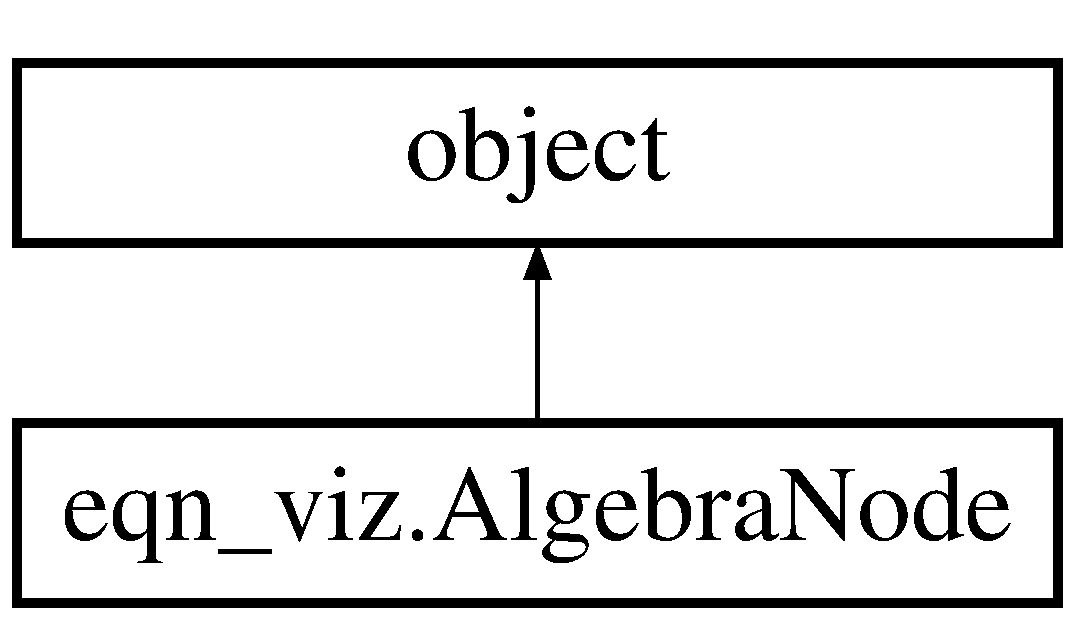
\includegraphics[height=2.000000cm]{classeqn__viz_1_1_algebra_node}
\end{center}
\end{figure}
\subsection*{Public Member Functions}
\begin{DoxyCompactItemize}
\item 
def \hyperlink{classeqn__viz_1_1_algebra_node_ae2acaafa5d5babb14e1e1ed4db9f26ae}{\+\_\+\+\_\+init\+\_\+\+\_\+} (self, \hyperlink{classeqn__viz_1_1_algebra_node_a6b8ed9f312eb416c8231f16b6abf77a0}{node\+\_\+name}, \hyperlink{classeqn__viz_1_1_algebra_node_aa6fa58662e30b03ed6eaf1039489297b}{children})
\item 
def \hyperlink{classeqn__viz_1_1_algebra_node_abebaa3c55c737a3759f6e673428c2af2}{convert\+Top\+Level\+Tree\+To\+Binary} (self)
\item 
def \hyperlink{classeqn__viz_1_1_algebra_node_ae91c975dfa9924ca629cad325f8b615c}{to\+Binary\+Tree} (self)
\item 
def \hyperlink{classeqn__viz_1_1_algebra_node_a58d4f89bf0f3f9c97c96e37a35f98f6d}{compress\+Bottom\+Two\+Children} (self)
\item 
def \hyperlink{classeqn__viz_1_1_algebra_node_aa55856a16de07e1966219d2d20ae1927}{tag\+Binary\+Tree} (self, current\+\_\+depth, node\+\_\+num)
\item 
def \hyperlink{classeqn__viz_1_1_algebra_node_a3fcf5aeaec65b3c3a19fa965a5b0eaf1}{old\+Tags\+And\+New\+Tags} (self)
\end{DoxyCompactItemize}
\subsection*{Public Attributes}
\begin{DoxyCompactItemize}
\item 
\hyperlink{classeqn__viz_1_1_algebra_node_aa6fa58662e30b03ed6eaf1039489297b}{children}
\item 
\hyperlink{classeqn__viz_1_1_algebra_node_a6b8ed9f312eb416c8231f16b6abf77a0}{node\+\_\+name}
\item 
\hyperlink{classeqn__viz_1_1_algebra_node_a9b40ad9a525b5421b76a525683793838}{new\+\_\+id}
\end{DoxyCompactItemize}


\subsection{Detailed Description}
\begin{DoxyVerb}encodes an algebra expression tree: used to convert node ids to binary tree format\end{DoxyVerb}
 

Definition at line 347 of file eqn\+\_\+viz.\+py.



\subsection{Constructor \& Destructor Documentation}
\hypertarget{classeqn__viz_1_1_algebra_node_ae2acaafa5d5babb14e1e1ed4db9f26ae}{}\index{eqn\+\_\+viz\+::\+Algebra\+Node@{eqn\+\_\+viz\+::\+Algebra\+Node}!\+\_\+\+\_\+init\+\_\+\+\_\+@{\+\_\+\+\_\+init\+\_\+\+\_\+}}
\index{\+\_\+\+\_\+init\+\_\+\+\_\+@{\+\_\+\+\_\+init\+\_\+\+\_\+}!eqn\+\_\+viz\+::\+Algebra\+Node@{eqn\+\_\+viz\+::\+Algebra\+Node}}
\subsubsection[{\+\_\+\+\_\+init\+\_\+\+\_\+}]{\setlength{\rightskip}{0pt plus 5cm}def eqn\+\_\+viz.\+Algebra\+Node.\+\_\+\+\_\+init\+\_\+\+\_\+ (
\begin{DoxyParamCaption}
\item[{}]{self, }
\item[{}]{node\+\_\+name, }
\item[{}]{children}
\end{DoxyParamCaption}
)}\label{classeqn__viz_1_1_algebra_node_ae2acaafa5d5babb14e1e1ed4db9f26ae}


Definition at line 349 of file eqn\+\_\+viz.\+py.



\subsection{Member Function Documentation}
\hypertarget{classeqn__viz_1_1_algebra_node_a58d4f89bf0f3f9c97c96e37a35f98f6d}{}\index{eqn\+\_\+viz\+::\+Algebra\+Node@{eqn\+\_\+viz\+::\+Algebra\+Node}!compress\+Bottom\+Two\+Children@{compress\+Bottom\+Two\+Children}}
\index{compress\+Bottom\+Two\+Children@{compress\+Bottom\+Two\+Children}!eqn\+\_\+viz\+::\+Algebra\+Node@{eqn\+\_\+viz\+::\+Algebra\+Node}}
\subsubsection[{compress\+Bottom\+Two\+Children}]{\setlength{\rightskip}{0pt plus 5cm}def eqn\+\_\+viz.\+Algebra\+Node.\+compress\+Bottom\+Two\+Children (
\begin{DoxyParamCaption}
\item[{}]{self}
\end{DoxyParamCaption}
)}\label{classeqn__viz_1_1_algebra_node_a58d4f89bf0f3f9c97c96e37a35f98f6d}


Definition at line 364 of file eqn\+\_\+viz.\+py.

\hypertarget{classeqn__viz_1_1_algebra_node_abebaa3c55c737a3759f6e673428c2af2}{}\index{eqn\+\_\+viz\+::\+Algebra\+Node@{eqn\+\_\+viz\+::\+Algebra\+Node}!convert\+Top\+Level\+Tree\+To\+Binary@{convert\+Top\+Level\+Tree\+To\+Binary}}
\index{convert\+Top\+Level\+Tree\+To\+Binary@{convert\+Top\+Level\+Tree\+To\+Binary}!eqn\+\_\+viz\+::\+Algebra\+Node@{eqn\+\_\+viz\+::\+Algebra\+Node}}
\subsubsection[{convert\+Top\+Level\+Tree\+To\+Binary}]{\setlength{\rightskip}{0pt plus 5cm}def eqn\+\_\+viz.\+Algebra\+Node.\+convert\+Top\+Level\+Tree\+To\+Binary (
\begin{DoxyParamCaption}
\item[{}]{self}
\end{DoxyParamCaption}
)}\label{classeqn__viz_1_1_algebra_node_abebaa3c55c737a3759f6e673428c2af2}


Definition at line 352 of file eqn\+\_\+viz.\+py.

\hypertarget{classeqn__viz_1_1_algebra_node_a3fcf5aeaec65b3c3a19fa965a5b0eaf1}{}\index{eqn\+\_\+viz\+::\+Algebra\+Node@{eqn\+\_\+viz\+::\+Algebra\+Node}!old\+Tags\+And\+New\+Tags@{old\+Tags\+And\+New\+Tags}}
\index{old\+Tags\+And\+New\+Tags@{old\+Tags\+And\+New\+Tags}!eqn\+\_\+viz\+::\+Algebra\+Node@{eqn\+\_\+viz\+::\+Algebra\+Node}}
\subsubsection[{old\+Tags\+And\+New\+Tags}]{\setlength{\rightskip}{0pt plus 5cm}def eqn\+\_\+viz.\+Algebra\+Node.\+old\+Tags\+And\+New\+Tags (
\begin{DoxyParamCaption}
\item[{}]{self}
\end{DoxyParamCaption}
)}\label{classeqn__viz_1_1_algebra_node_a3fcf5aeaec65b3c3a19fa965a5b0eaf1}


Definition at line 379 of file eqn\+\_\+viz.\+py.

\hypertarget{classeqn__viz_1_1_algebra_node_aa55856a16de07e1966219d2d20ae1927}{}\index{eqn\+\_\+viz\+::\+Algebra\+Node@{eqn\+\_\+viz\+::\+Algebra\+Node}!tag\+Binary\+Tree@{tag\+Binary\+Tree}}
\index{tag\+Binary\+Tree@{tag\+Binary\+Tree}!eqn\+\_\+viz\+::\+Algebra\+Node@{eqn\+\_\+viz\+::\+Algebra\+Node}}
\subsubsection[{tag\+Binary\+Tree}]{\setlength{\rightskip}{0pt plus 5cm}def eqn\+\_\+viz.\+Algebra\+Node.\+tag\+Binary\+Tree (
\begin{DoxyParamCaption}
\item[{}]{self, }
\item[{}]{current\+\_\+depth, }
\item[{}]{node\+\_\+num}
\end{DoxyParamCaption}
)}\label{classeqn__viz_1_1_algebra_node_aa55856a16de07e1966219d2d20ae1927}


Definition at line 371 of file eqn\+\_\+viz.\+py.

\hypertarget{classeqn__viz_1_1_algebra_node_ae91c975dfa9924ca629cad325f8b615c}{}\index{eqn\+\_\+viz\+::\+Algebra\+Node@{eqn\+\_\+viz\+::\+Algebra\+Node}!to\+Binary\+Tree@{to\+Binary\+Tree}}
\index{to\+Binary\+Tree@{to\+Binary\+Tree}!eqn\+\_\+viz\+::\+Algebra\+Node@{eqn\+\_\+viz\+::\+Algebra\+Node}}
\subsubsection[{to\+Binary\+Tree}]{\setlength{\rightskip}{0pt plus 5cm}def eqn\+\_\+viz.\+Algebra\+Node.\+to\+Binary\+Tree (
\begin{DoxyParamCaption}
\item[{}]{self}
\end{DoxyParamCaption}
)}\label{classeqn__viz_1_1_algebra_node_ae91c975dfa9924ca629cad325f8b615c}


Definition at line 358 of file eqn\+\_\+viz.\+py.



\subsection{Member Data Documentation}
\hypertarget{classeqn__viz_1_1_algebra_node_aa6fa58662e30b03ed6eaf1039489297b}{}\index{eqn\+\_\+viz\+::\+Algebra\+Node@{eqn\+\_\+viz\+::\+Algebra\+Node}!children@{children}}
\index{children@{children}!eqn\+\_\+viz\+::\+Algebra\+Node@{eqn\+\_\+viz\+::\+Algebra\+Node}}
\subsubsection[{children}]{\setlength{\rightskip}{0pt plus 5cm}eqn\+\_\+viz.\+Algebra\+Node.\+children}\label{classeqn__viz_1_1_algebra_node_aa6fa58662e30b03ed6eaf1039489297b}


Definition at line 351 of file eqn\+\_\+viz.\+py.

\hypertarget{classeqn__viz_1_1_algebra_node_a9b40ad9a525b5421b76a525683793838}{}\index{eqn\+\_\+viz\+::\+Algebra\+Node@{eqn\+\_\+viz\+::\+Algebra\+Node}!new\+\_\+id@{new\+\_\+id}}
\index{new\+\_\+id@{new\+\_\+id}!eqn\+\_\+viz\+::\+Algebra\+Node@{eqn\+\_\+viz\+::\+Algebra\+Node}}
\subsubsection[{new\+\_\+id}]{\setlength{\rightskip}{0pt plus 5cm}eqn\+\_\+viz.\+Algebra\+Node.\+new\+\_\+id}\label{classeqn__viz_1_1_algebra_node_a9b40ad9a525b5421b76a525683793838}


Definition at line 372 of file eqn\+\_\+viz.\+py.

\hypertarget{classeqn__viz_1_1_algebra_node_a6b8ed9f312eb416c8231f16b6abf77a0}{}\index{eqn\+\_\+viz\+::\+Algebra\+Node@{eqn\+\_\+viz\+::\+Algebra\+Node}!node\+\_\+name@{node\+\_\+name}}
\index{node\+\_\+name@{node\+\_\+name}!eqn\+\_\+viz\+::\+Algebra\+Node@{eqn\+\_\+viz\+::\+Algebra\+Node}}
\subsubsection[{node\+\_\+name}]{\setlength{\rightskip}{0pt plus 5cm}eqn\+\_\+viz.\+Algebra\+Node.\+node\+\_\+name}\label{classeqn__viz_1_1_algebra_node_a6b8ed9f312eb416c8231f16b6abf77a0}


Definition at line 354 of file eqn\+\_\+viz.\+py.



The documentation for this class was generated from the following file\+:\begin{DoxyCompactItemize}
\item 
\hyperlink{eqn__viz_8py}{eqn\+\_\+viz.\+py}\end{DoxyCompactItemize}

\hypertarget{classtranslate__tree__nodes_1_1_algebra_node}{}\section{translate\+\_\+tree\+\_\+nodes.\+Algebra\+Node Class Reference}
\label{classtranslate__tree__nodes_1_1_algebra_node}\index{translate\+\_\+tree\+\_\+nodes.\+Algebra\+Node@{translate\+\_\+tree\+\_\+nodes.\+Algebra\+Node}}
\subsection*{Public Member Functions}
\begin{DoxyCompactItemize}
\item 
def \hyperlink{classtranslate__tree__nodes_1_1_algebra_node_a9ac9e8b3121983d70eaca4aca26fc4fc}{\+\_\+\+\_\+init\+\_\+\+\_\+} (self, \hyperlink{classtranslate__tree__nodes_1_1_algebra_node_a1ce43e48160b84abc8847aac2daad122}{node\+\_\+name}, \hyperlink{classtranslate__tree__nodes_1_1_algebra_node_a03cc9dbcddb31a4b06f23b73046ee1d1}{children})
\item 
def \hyperlink{classtranslate__tree__nodes_1_1_algebra_node_a2505974def9029fda0d6ec1b3817853c}{convert\+Top\+Level\+Tree\+To\+Binary} (self)
\item 
def \hyperlink{classtranslate__tree__nodes_1_1_algebra_node_a253cbbed2e99544970f8b6cc332ef2e2}{to\+Binary\+Tree} (self)
\item 
def \hyperlink{classtranslate__tree__nodes_1_1_algebra_node_afbe5fdb0be62d22236ff698f9d969e63}{compress\+Bottom\+Two\+Children} (self)
\item 
def \hyperlink{classtranslate__tree__nodes_1_1_algebra_node_a628ca06aad3a58b8fe8215a7413c3e37}{to\+String}
\item 
def \hyperlink{classtranslate__tree__nodes_1_1_algebra_node_af97750d7635c161a5ac8c05fc0a066f0}{\+\_\+\+\_\+str\+\_\+\+\_\+} (self)
\item 
def \hyperlink{classtranslate__tree__nodes_1_1_algebra_node_a91ef0fed00104f4478df988e16937dbc}{tag\+Binary\+Tree} (self, current\+\_\+depth, node\+\_\+num)
\item 
def \hyperlink{classtranslate__tree__nodes_1_1_algebra_node_a39d416c5e3373e2074831354afc9a067}{old\+Tags\+And\+New\+Tags} (self)
\end{DoxyCompactItemize}
\subsection*{Public Attributes}
\begin{DoxyCompactItemize}
\item 
\hyperlink{classtranslate__tree__nodes_1_1_algebra_node_a03cc9dbcddb31a4b06f23b73046ee1d1}{children}
\item 
\hyperlink{classtranslate__tree__nodes_1_1_algebra_node_a1ce43e48160b84abc8847aac2daad122}{node\+\_\+name}
\item 
\hyperlink{classtranslate__tree__nodes_1_1_algebra_node_ae5b55b8b4bc4eb136d1f056e04419e78}{new\+\_\+id}
\end{DoxyCompactItemize}


\subsection{Detailed Description}
\begin{DoxyVerb}encodes an algebra expression tree: used to convert node ids to binary tree format\end{DoxyVerb}
 

Definition at line 37 of file translate\+\_\+tree\+\_\+nodes.\+py.



\subsection{Constructor \& Destructor Documentation}
\hypertarget{classtranslate__tree__nodes_1_1_algebra_node_a9ac9e8b3121983d70eaca4aca26fc4fc}{}\index{translate\+\_\+tree\+\_\+nodes\+::\+Algebra\+Node@{translate\+\_\+tree\+\_\+nodes\+::\+Algebra\+Node}!\+\_\+\+\_\+init\+\_\+\+\_\+@{\+\_\+\+\_\+init\+\_\+\+\_\+}}
\index{\+\_\+\+\_\+init\+\_\+\+\_\+@{\+\_\+\+\_\+init\+\_\+\+\_\+}!translate\+\_\+tree\+\_\+nodes\+::\+Algebra\+Node@{translate\+\_\+tree\+\_\+nodes\+::\+Algebra\+Node}}
\subsubsection[{\+\_\+\+\_\+init\+\_\+\+\_\+}]{\setlength{\rightskip}{0pt plus 5cm}def translate\+\_\+tree\+\_\+nodes.\+Algebra\+Node.\+\_\+\+\_\+init\+\_\+\+\_\+ (
\begin{DoxyParamCaption}
\item[{}]{self, }
\item[{}]{node\+\_\+name, }
\item[{}]{children}
\end{DoxyParamCaption}
)}\label{classtranslate__tree__nodes_1_1_algebra_node_a9ac9e8b3121983d70eaca4aca26fc4fc}


Definition at line 39 of file translate\+\_\+tree\+\_\+nodes.\+py.



\subsection{Member Function Documentation}
\hypertarget{classtranslate__tree__nodes_1_1_algebra_node_af97750d7635c161a5ac8c05fc0a066f0}{}\index{translate\+\_\+tree\+\_\+nodes\+::\+Algebra\+Node@{translate\+\_\+tree\+\_\+nodes\+::\+Algebra\+Node}!\+\_\+\+\_\+str\+\_\+\+\_\+@{\+\_\+\+\_\+str\+\_\+\+\_\+}}
\index{\+\_\+\+\_\+str\+\_\+\+\_\+@{\+\_\+\+\_\+str\+\_\+\+\_\+}!translate\+\_\+tree\+\_\+nodes\+::\+Algebra\+Node@{translate\+\_\+tree\+\_\+nodes\+::\+Algebra\+Node}}
\subsubsection[{\+\_\+\+\_\+str\+\_\+\+\_\+}]{\setlength{\rightskip}{0pt plus 5cm}def translate\+\_\+tree\+\_\+nodes.\+Algebra\+Node.\+\_\+\+\_\+str\+\_\+\+\_\+ (
\begin{DoxyParamCaption}
\item[{}]{self}
\end{DoxyParamCaption}
)}\label{classtranslate__tree__nodes_1_1_algebra_node_af97750d7635c161a5ac8c05fc0a066f0}


Definition at line 67 of file translate\+\_\+tree\+\_\+nodes.\+py.

\hypertarget{classtranslate__tree__nodes_1_1_algebra_node_afbe5fdb0be62d22236ff698f9d969e63}{}\index{translate\+\_\+tree\+\_\+nodes\+::\+Algebra\+Node@{translate\+\_\+tree\+\_\+nodes\+::\+Algebra\+Node}!compress\+Bottom\+Two\+Children@{compress\+Bottom\+Two\+Children}}
\index{compress\+Bottom\+Two\+Children@{compress\+Bottom\+Two\+Children}!translate\+\_\+tree\+\_\+nodes\+::\+Algebra\+Node@{translate\+\_\+tree\+\_\+nodes\+::\+Algebra\+Node}}
\subsubsection[{compress\+Bottom\+Two\+Children}]{\setlength{\rightskip}{0pt plus 5cm}def translate\+\_\+tree\+\_\+nodes.\+Algebra\+Node.\+compress\+Bottom\+Two\+Children (
\begin{DoxyParamCaption}
\item[{}]{self}
\end{DoxyParamCaption}
)}\label{classtranslate__tree__nodes_1_1_algebra_node_afbe5fdb0be62d22236ff698f9d969e63}


Definition at line 53 of file translate\+\_\+tree\+\_\+nodes.\+py.

\hypertarget{classtranslate__tree__nodes_1_1_algebra_node_a2505974def9029fda0d6ec1b3817853c}{}\index{translate\+\_\+tree\+\_\+nodes\+::\+Algebra\+Node@{translate\+\_\+tree\+\_\+nodes\+::\+Algebra\+Node}!convert\+Top\+Level\+Tree\+To\+Binary@{convert\+Top\+Level\+Tree\+To\+Binary}}
\index{convert\+Top\+Level\+Tree\+To\+Binary@{convert\+Top\+Level\+Tree\+To\+Binary}!translate\+\_\+tree\+\_\+nodes\+::\+Algebra\+Node@{translate\+\_\+tree\+\_\+nodes\+::\+Algebra\+Node}}
\subsubsection[{convert\+Top\+Level\+Tree\+To\+Binary}]{\setlength{\rightskip}{0pt plus 5cm}def translate\+\_\+tree\+\_\+nodes.\+Algebra\+Node.\+convert\+Top\+Level\+Tree\+To\+Binary (
\begin{DoxyParamCaption}
\item[{}]{self}
\end{DoxyParamCaption}
)}\label{classtranslate__tree__nodes_1_1_algebra_node_a2505974def9029fda0d6ec1b3817853c}


Definition at line 41 of file translate\+\_\+tree\+\_\+nodes.\+py.

\hypertarget{classtranslate__tree__nodes_1_1_algebra_node_a39d416c5e3373e2074831354afc9a067}{}\index{translate\+\_\+tree\+\_\+nodes\+::\+Algebra\+Node@{translate\+\_\+tree\+\_\+nodes\+::\+Algebra\+Node}!old\+Tags\+And\+New\+Tags@{old\+Tags\+And\+New\+Tags}}
\index{old\+Tags\+And\+New\+Tags@{old\+Tags\+And\+New\+Tags}!translate\+\_\+tree\+\_\+nodes\+::\+Algebra\+Node@{translate\+\_\+tree\+\_\+nodes\+::\+Algebra\+Node}}
\subsubsection[{old\+Tags\+And\+New\+Tags}]{\setlength{\rightskip}{0pt plus 5cm}def translate\+\_\+tree\+\_\+nodes.\+Algebra\+Node.\+old\+Tags\+And\+New\+Tags (
\begin{DoxyParamCaption}
\item[{}]{self}
\end{DoxyParamCaption}
)}\label{classtranslate__tree__nodes_1_1_algebra_node_a39d416c5e3373e2074831354afc9a067}


Definition at line 78 of file translate\+\_\+tree\+\_\+nodes.\+py.

\hypertarget{classtranslate__tree__nodes_1_1_algebra_node_a91ef0fed00104f4478df988e16937dbc}{}\index{translate\+\_\+tree\+\_\+nodes\+::\+Algebra\+Node@{translate\+\_\+tree\+\_\+nodes\+::\+Algebra\+Node}!tag\+Binary\+Tree@{tag\+Binary\+Tree}}
\index{tag\+Binary\+Tree@{tag\+Binary\+Tree}!translate\+\_\+tree\+\_\+nodes\+::\+Algebra\+Node@{translate\+\_\+tree\+\_\+nodes\+::\+Algebra\+Node}}
\subsubsection[{tag\+Binary\+Tree}]{\setlength{\rightskip}{0pt plus 5cm}def translate\+\_\+tree\+\_\+nodes.\+Algebra\+Node.\+tag\+Binary\+Tree (
\begin{DoxyParamCaption}
\item[{}]{self, }
\item[{}]{current\+\_\+depth, }
\item[{}]{node\+\_\+num}
\end{DoxyParamCaption}
)}\label{classtranslate__tree__nodes_1_1_algebra_node_a91ef0fed00104f4478df988e16937dbc}


Definition at line 70 of file translate\+\_\+tree\+\_\+nodes.\+py.

\hypertarget{classtranslate__tree__nodes_1_1_algebra_node_a253cbbed2e99544970f8b6cc332ef2e2}{}\index{translate\+\_\+tree\+\_\+nodes\+::\+Algebra\+Node@{translate\+\_\+tree\+\_\+nodes\+::\+Algebra\+Node}!to\+Binary\+Tree@{to\+Binary\+Tree}}
\index{to\+Binary\+Tree@{to\+Binary\+Tree}!translate\+\_\+tree\+\_\+nodes\+::\+Algebra\+Node@{translate\+\_\+tree\+\_\+nodes\+::\+Algebra\+Node}}
\subsubsection[{to\+Binary\+Tree}]{\setlength{\rightskip}{0pt plus 5cm}def translate\+\_\+tree\+\_\+nodes.\+Algebra\+Node.\+to\+Binary\+Tree (
\begin{DoxyParamCaption}
\item[{}]{self}
\end{DoxyParamCaption}
)}\label{classtranslate__tree__nodes_1_1_algebra_node_a253cbbed2e99544970f8b6cc332ef2e2}


Definition at line 47 of file translate\+\_\+tree\+\_\+nodes.\+py.

\hypertarget{classtranslate__tree__nodes_1_1_algebra_node_a628ca06aad3a58b8fe8215a7413c3e37}{}\index{translate\+\_\+tree\+\_\+nodes\+::\+Algebra\+Node@{translate\+\_\+tree\+\_\+nodes\+::\+Algebra\+Node}!to\+String@{to\+String}}
\index{to\+String@{to\+String}!translate\+\_\+tree\+\_\+nodes\+::\+Algebra\+Node@{translate\+\_\+tree\+\_\+nodes\+::\+Algebra\+Node}}
\subsubsection[{to\+String}]{\setlength{\rightskip}{0pt plus 5cm}def translate\+\_\+tree\+\_\+nodes.\+Algebra\+Node.\+to\+String (
\begin{DoxyParamCaption}
\item[{}]{self, }
\item[{}]{depth = {\ttfamily 0}}
\end{DoxyParamCaption}
)}\label{classtranslate__tree__nodes_1_1_algebra_node_a628ca06aad3a58b8fe8215a7413c3e37}


Definition at line 61 of file translate\+\_\+tree\+\_\+nodes.\+py.



\subsection{Member Data Documentation}
\hypertarget{classtranslate__tree__nodes_1_1_algebra_node_a03cc9dbcddb31a4b06f23b73046ee1d1}{}\index{translate\+\_\+tree\+\_\+nodes\+::\+Algebra\+Node@{translate\+\_\+tree\+\_\+nodes\+::\+Algebra\+Node}!children@{children}}
\index{children@{children}!translate\+\_\+tree\+\_\+nodes\+::\+Algebra\+Node@{translate\+\_\+tree\+\_\+nodes\+::\+Algebra\+Node}}
\subsubsection[{children}]{\setlength{\rightskip}{0pt plus 5cm}translate\+\_\+tree\+\_\+nodes.\+Algebra\+Node.\+children}\label{classtranslate__tree__nodes_1_1_algebra_node_a03cc9dbcddb31a4b06f23b73046ee1d1}


Definition at line 40 of file translate\+\_\+tree\+\_\+nodes.\+py.

\hypertarget{classtranslate__tree__nodes_1_1_algebra_node_ae5b55b8b4bc4eb136d1f056e04419e78}{}\index{translate\+\_\+tree\+\_\+nodes\+::\+Algebra\+Node@{translate\+\_\+tree\+\_\+nodes\+::\+Algebra\+Node}!new\+\_\+id@{new\+\_\+id}}
\index{new\+\_\+id@{new\+\_\+id}!translate\+\_\+tree\+\_\+nodes\+::\+Algebra\+Node@{translate\+\_\+tree\+\_\+nodes\+::\+Algebra\+Node}}
\subsubsection[{new\+\_\+id}]{\setlength{\rightskip}{0pt plus 5cm}translate\+\_\+tree\+\_\+nodes.\+Algebra\+Node.\+new\+\_\+id}\label{classtranslate__tree__nodes_1_1_algebra_node_ae5b55b8b4bc4eb136d1f056e04419e78}


Definition at line 71 of file translate\+\_\+tree\+\_\+nodes.\+py.

\hypertarget{classtranslate__tree__nodes_1_1_algebra_node_a1ce43e48160b84abc8847aac2daad122}{}\index{translate\+\_\+tree\+\_\+nodes\+::\+Algebra\+Node@{translate\+\_\+tree\+\_\+nodes\+::\+Algebra\+Node}!node\+\_\+name@{node\+\_\+name}}
\index{node\+\_\+name@{node\+\_\+name}!translate\+\_\+tree\+\_\+nodes\+::\+Algebra\+Node@{translate\+\_\+tree\+\_\+nodes\+::\+Algebra\+Node}}
\subsubsection[{node\+\_\+name}]{\setlength{\rightskip}{0pt plus 5cm}translate\+\_\+tree\+\_\+nodes.\+Algebra\+Node.\+node\+\_\+name}\label{classtranslate__tree__nodes_1_1_algebra_node_a1ce43e48160b84abc8847aac2daad122}


Definition at line 43 of file translate\+\_\+tree\+\_\+nodes.\+py.



The documentation for this class was generated from the following file\+:\begin{DoxyCompactItemize}
\item 
\hyperlink{translate__tree__nodes_8py}{translate\+\_\+tree\+\_\+nodes.\+py}\end{DoxyCompactItemize}

\hypertarget{classtotally__new__visualizer_1_1_answer_set_j_s_o_n_encoder}{}\section{totally\+\_\+new\+\_\+visualizer.\+Answer\+Set\+J\+S\+O\+N\+Encoder Class Reference}
\label{classtotally__new__visualizer_1_1_answer_set_j_s_o_n_encoder}\index{totally\+\_\+new\+\_\+visualizer.\+Answer\+Set\+J\+S\+O\+N\+Encoder@{totally\+\_\+new\+\_\+visualizer.\+Answer\+Set\+J\+S\+O\+N\+Encoder}}
Inheritance diagram for totally\+\_\+new\+\_\+visualizer.\+Answer\+Set\+J\+S\+O\+N\+Encoder\+:\begin{figure}[H]
\begin{center}
\leavevmode
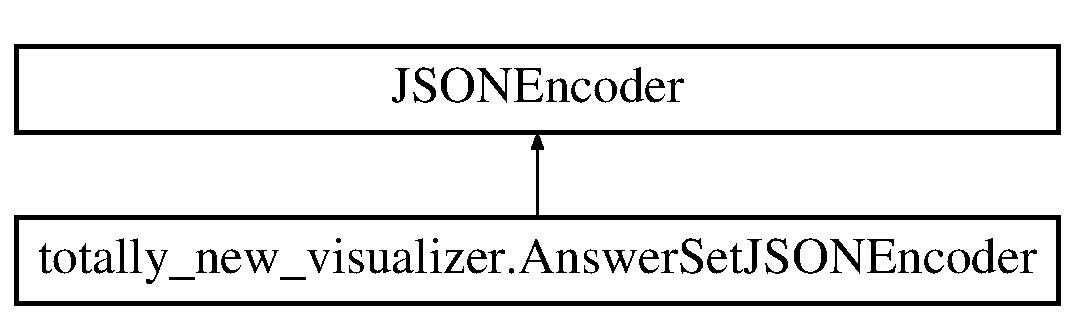
\includegraphics[height=2.000000cm]{classtotally__new__visualizer_1_1_answer_set_j_s_o_n_encoder}
\end{center}
\end{figure}
\subsection*{Public Member Functions}
\begin{DoxyCompactItemize}
\item 
def \hyperlink{classtotally__new__visualizer_1_1_answer_set_j_s_o_n_encoder_a104cc50e2ac18448721cdf608aef3c90}{default} (self, ans\+\_\+set\+\_\+mgr)
\item 
def \hyperlink{classtotally__new__visualizer_1_1_answer_set_j_s_o_n_encoder_a9426d9aabb2c10aa95cd64fd7535ddfb}{encode\+Single\+Problem} (self, problem)
\item 
def \hyperlink{classtotally__new__visualizer_1_1_answer_set_j_s_o_n_encoder_a2aff8b46377f69068f2b96a61a3225dd}{encode\+Single\+Solution} (self, solution)
\end{DoxyCompactItemize}


\subsection{Detailed Description}


Definition at line 433 of file totally\+\_\+new\+\_\+visualizer.\+py.



\subsection{Member Function Documentation}
\hypertarget{classtotally__new__visualizer_1_1_answer_set_j_s_o_n_encoder_a104cc50e2ac18448721cdf608aef3c90}{}\index{totally\+\_\+new\+\_\+visualizer\+::\+Answer\+Set\+J\+S\+O\+N\+Encoder@{totally\+\_\+new\+\_\+visualizer\+::\+Answer\+Set\+J\+S\+O\+N\+Encoder}!default@{default}}
\index{default@{default}!totally\+\_\+new\+\_\+visualizer\+::\+Answer\+Set\+J\+S\+O\+N\+Encoder@{totally\+\_\+new\+\_\+visualizer\+::\+Answer\+Set\+J\+S\+O\+N\+Encoder}}
\subsubsection[{default}]{\setlength{\rightskip}{0pt plus 5cm}def totally\+\_\+new\+\_\+visualizer.\+Answer\+Set\+J\+S\+O\+N\+Encoder.\+default (
\begin{DoxyParamCaption}
\item[{}]{self, }
\item[{}]{ans\+\_\+set\+\_\+mgr}
\end{DoxyParamCaption}
)}\label{classtotally__new__visualizer_1_1_answer_set_j_s_o_n_encoder_a104cc50e2ac18448721cdf608aef3c90}


Definition at line 434 of file totally\+\_\+new\+\_\+visualizer.\+py.

\hypertarget{classtotally__new__visualizer_1_1_answer_set_j_s_o_n_encoder_a9426d9aabb2c10aa95cd64fd7535ddfb}{}\index{totally\+\_\+new\+\_\+visualizer\+::\+Answer\+Set\+J\+S\+O\+N\+Encoder@{totally\+\_\+new\+\_\+visualizer\+::\+Answer\+Set\+J\+S\+O\+N\+Encoder}!encode\+Single\+Problem@{encode\+Single\+Problem}}
\index{encode\+Single\+Problem@{encode\+Single\+Problem}!totally\+\_\+new\+\_\+visualizer\+::\+Answer\+Set\+J\+S\+O\+N\+Encoder@{totally\+\_\+new\+\_\+visualizer\+::\+Answer\+Set\+J\+S\+O\+N\+Encoder}}
\subsubsection[{encode\+Single\+Problem}]{\setlength{\rightskip}{0pt plus 5cm}def totally\+\_\+new\+\_\+visualizer.\+Answer\+Set\+J\+S\+O\+N\+Encoder.\+encode\+Single\+Problem (
\begin{DoxyParamCaption}
\item[{}]{self, }
\item[{}]{problem}
\end{DoxyParamCaption}
)}\label{classtotally__new__visualizer_1_1_answer_set_j_s_o_n_encoder_a9426d9aabb2c10aa95cd64fd7535ddfb}


Definition at line 440 of file totally\+\_\+new\+\_\+visualizer.\+py.

\hypertarget{classtotally__new__visualizer_1_1_answer_set_j_s_o_n_encoder_a2aff8b46377f69068f2b96a61a3225dd}{}\index{totally\+\_\+new\+\_\+visualizer\+::\+Answer\+Set\+J\+S\+O\+N\+Encoder@{totally\+\_\+new\+\_\+visualizer\+::\+Answer\+Set\+J\+S\+O\+N\+Encoder}!encode\+Single\+Solution@{encode\+Single\+Solution}}
\index{encode\+Single\+Solution@{encode\+Single\+Solution}!totally\+\_\+new\+\_\+visualizer\+::\+Answer\+Set\+J\+S\+O\+N\+Encoder@{totally\+\_\+new\+\_\+visualizer\+::\+Answer\+Set\+J\+S\+O\+N\+Encoder}}
\subsubsection[{encode\+Single\+Solution}]{\setlength{\rightskip}{0pt plus 5cm}def totally\+\_\+new\+\_\+visualizer.\+Answer\+Set\+J\+S\+O\+N\+Encoder.\+encode\+Single\+Solution (
\begin{DoxyParamCaption}
\item[{}]{self, }
\item[{}]{solution}
\end{DoxyParamCaption}
)}\label{classtotally__new__visualizer_1_1_answer_set_j_s_o_n_encoder_a2aff8b46377f69068f2b96a61a3225dd}


Definition at line 442 of file totally\+\_\+new\+\_\+visualizer.\+py.



The documentation for this class was generated from the following file\+:\begin{DoxyCompactItemize}
\item 
\hyperlink{totally__new__visualizer_8py}{totally\+\_\+new\+\_\+visualizer.\+py}\end{DoxyCompactItemize}

\hypertarget{classeqn__viz_1_1_answer_set_manager}{}\section{eqn\+\_\+viz.\+Answer\+Set\+Manager Class Reference}
\label{classeqn__viz_1_1_answer_set_manager}\index{eqn\+\_\+viz.\+Answer\+Set\+Manager@{eqn\+\_\+viz.\+Answer\+Set\+Manager}}
Inheritance diagram for eqn\+\_\+viz.\+Answer\+Set\+Manager\+:\begin{figure}[H]
\begin{center}
\leavevmode
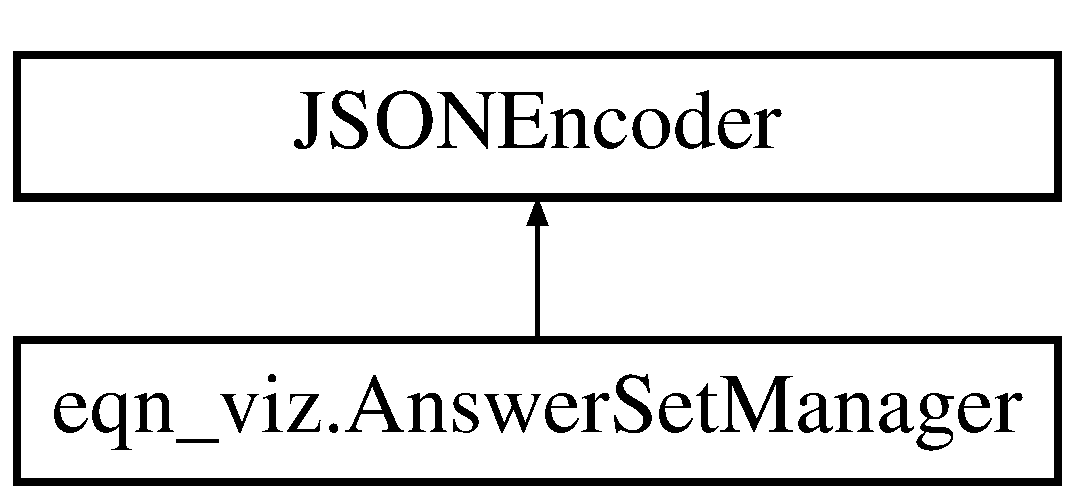
\includegraphics[height=2.000000cm]{classeqn__viz_1_1_answer_set_manager}
\end{center}
\end{figure}
\subsection*{Public Member Functions}
\begin{DoxyCompactItemize}
\item 
def \hyperlink{classeqn__viz_1_1_answer_set_manager_a9bd9622d26fa24a188a825d2b5137b13}{\+\_\+\+\_\+init\+\_\+\+\_\+} (self, \hyperlink{classeqn__viz_1_1_answer_set_manager_a15d9c03574ab43af95dc420cb125df11}{cmdline\+\_\+args})
\item 
def \hyperlink{classeqn__viz_1_1_answer_set_manager_a66cb1f21deee1507810d80f670bcdeb7}{get\+Generated\+Ans\+Sets} (self)
\item 
def \hyperlink{classeqn__viz_1_1_answer_set_manager_a54a34f14351d91c57ca1a0fb5292959b}{get\+Generated\+Problems} (self)
\item 
def \hyperlink{classeqn__viz_1_1_answer_set_manager_ac9d5c0d89ad8693ed7c31df75d61c8c7}{init\+From\+S\+T\+D\+I\+N} (self)
\item 
def \hyperlink{classeqn__viz_1_1_answer_set_manager_a61acb8db5bc5cb6bdf9300016fc21a60}{default} (self, answer\+\_\+set)
\item 
def \hyperlink{classeqn__viz_1_1_answer_set_manager_a9ac22e2d51a183ee9ad9eeb928ab1a1c}{init\+From\+J\+S\+O\+N\+File} (self, file\+\_\+name)
\item 
def \hyperlink{classeqn__viz_1_1_answer_set_manager_a3e89932b2df88cc458570b1e88f587df}{get\+Ans\+Sets\+As\+J\+S\+O\+N} (self)
\item 
def \hyperlink{classeqn__viz_1_1_answer_set_manager_ae3c8a041865a03bb4d521a59064aaaf1}{print\+Answer\+Sets}
\end{DoxyCompactItemize}
\subsection*{Public Attributes}
\begin{DoxyCompactItemize}
\item 
\hyperlink{classeqn__viz_1_1_answer_set_manager_a15d9c03574ab43af95dc420cb125df11}{cmdline\+\_\+args}
\item 
\hyperlink{classeqn__viz_1_1_answer_set_manager_ab50545866708c615d07364479ab771e5}{answer\+\_\+sets}
\end{DoxyCompactItemize}


\subsection{Detailed Description}
\begin{DoxyVerb}This class parses answer sets from stdin or json file, outputs to file in json format or user-friendly format\end{DoxyVerb}
 

Definition at line 677 of file eqn\+\_\+viz.\+py.



\subsection{Constructor \& Destructor Documentation}
\hypertarget{classeqn__viz_1_1_answer_set_manager_a9bd9622d26fa24a188a825d2b5137b13}{}\index{eqn\+\_\+viz\+::\+Answer\+Set\+Manager@{eqn\+\_\+viz\+::\+Answer\+Set\+Manager}!\+\_\+\+\_\+init\+\_\+\+\_\+@{\+\_\+\+\_\+init\+\_\+\+\_\+}}
\index{\+\_\+\+\_\+init\+\_\+\+\_\+@{\+\_\+\+\_\+init\+\_\+\+\_\+}!eqn\+\_\+viz\+::\+Answer\+Set\+Manager@{eqn\+\_\+viz\+::\+Answer\+Set\+Manager}}
\subsubsection[{\+\_\+\+\_\+init\+\_\+\+\_\+}]{\setlength{\rightskip}{0pt plus 5cm}def eqn\+\_\+viz.\+Answer\+Set\+Manager.\+\_\+\+\_\+init\+\_\+\+\_\+ (
\begin{DoxyParamCaption}
\item[{}]{self, }
\item[{}]{cmdline\+\_\+args}
\end{DoxyParamCaption}
)}\label{classeqn__viz_1_1_answer_set_manager_a9bd9622d26fa24a188a825d2b5137b13}


Definition at line 679 of file eqn\+\_\+viz.\+py.



\subsection{Member Function Documentation}
\hypertarget{classeqn__viz_1_1_answer_set_manager_a61acb8db5bc5cb6bdf9300016fc21a60}{}\index{eqn\+\_\+viz\+::\+Answer\+Set\+Manager@{eqn\+\_\+viz\+::\+Answer\+Set\+Manager}!default@{default}}
\index{default@{default}!eqn\+\_\+viz\+::\+Answer\+Set\+Manager@{eqn\+\_\+viz\+::\+Answer\+Set\+Manager}}
\subsubsection[{default}]{\setlength{\rightskip}{0pt plus 5cm}def eqn\+\_\+viz.\+Answer\+Set\+Manager.\+default (
\begin{DoxyParamCaption}
\item[{}]{self, }
\item[{}]{answer\+\_\+set}
\end{DoxyParamCaption}
)}\label{classeqn__viz_1_1_answer_set_manager_a61acb8db5bc5cb6bdf9300016fc21a60}
\begin{DoxyVerb}:param answer_set: answers set to save
:return: json encoded answer set (a string)
\end{DoxyVerb}
 

Definition at line 710 of file eqn\+\_\+viz.\+py.

\hypertarget{classeqn__viz_1_1_answer_set_manager_a3e89932b2df88cc458570b1e88f587df}{}\index{eqn\+\_\+viz\+::\+Answer\+Set\+Manager@{eqn\+\_\+viz\+::\+Answer\+Set\+Manager}!get\+Ans\+Sets\+As\+J\+S\+O\+N@{get\+Ans\+Sets\+As\+J\+S\+O\+N}}
\index{get\+Ans\+Sets\+As\+J\+S\+O\+N@{get\+Ans\+Sets\+As\+J\+S\+O\+N}!eqn\+\_\+viz\+::\+Answer\+Set\+Manager@{eqn\+\_\+viz\+::\+Answer\+Set\+Manager}}
\subsubsection[{get\+Ans\+Sets\+As\+J\+S\+O\+N}]{\setlength{\rightskip}{0pt plus 5cm}def eqn\+\_\+viz.\+Answer\+Set\+Manager.\+get\+Ans\+Sets\+As\+J\+S\+O\+N (
\begin{DoxyParamCaption}
\item[{}]{self}
\end{DoxyParamCaption}
)}\label{classeqn__viz_1_1_answer_set_manager_a3e89932b2df88cc458570b1e88f587df}


Definition at line 733 of file eqn\+\_\+viz.\+py.

\hypertarget{classeqn__viz_1_1_answer_set_manager_a66cb1f21deee1507810d80f670bcdeb7}{}\index{eqn\+\_\+viz\+::\+Answer\+Set\+Manager@{eqn\+\_\+viz\+::\+Answer\+Set\+Manager}!get\+Generated\+Ans\+Sets@{get\+Generated\+Ans\+Sets}}
\index{get\+Generated\+Ans\+Sets@{get\+Generated\+Ans\+Sets}!eqn\+\_\+viz\+::\+Answer\+Set\+Manager@{eqn\+\_\+viz\+::\+Answer\+Set\+Manager}}
\subsubsection[{get\+Generated\+Ans\+Sets}]{\setlength{\rightskip}{0pt plus 5cm}def eqn\+\_\+viz.\+Answer\+Set\+Manager.\+get\+Generated\+Ans\+Sets (
\begin{DoxyParamCaption}
\item[{}]{self}
\end{DoxyParamCaption}
)}\label{classeqn__viz_1_1_answer_set_manager_a66cb1f21deee1507810d80f670bcdeb7}


Definition at line 686 of file eqn\+\_\+viz.\+py.

\hypertarget{classeqn__viz_1_1_answer_set_manager_a54a34f14351d91c57ca1a0fb5292959b}{}\index{eqn\+\_\+viz\+::\+Answer\+Set\+Manager@{eqn\+\_\+viz\+::\+Answer\+Set\+Manager}!get\+Generated\+Problems@{get\+Generated\+Problems}}
\index{get\+Generated\+Problems@{get\+Generated\+Problems}!eqn\+\_\+viz\+::\+Answer\+Set\+Manager@{eqn\+\_\+viz\+::\+Answer\+Set\+Manager}}
\subsubsection[{get\+Generated\+Problems}]{\setlength{\rightskip}{0pt plus 5cm}def eqn\+\_\+viz.\+Answer\+Set\+Manager.\+get\+Generated\+Problems (
\begin{DoxyParamCaption}
\item[{}]{self}
\end{DoxyParamCaption}
)}\label{classeqn__viz_1_1_answer_set_manager_a54a34f14351d91c57ca1a0fb5292959b}
\begin{DoxyVerb}returns a flat list of all problems contained by answer set manager\end{DoxyVerb}
 

Definition at line 688 of file eqn\+\_\+viz.\+py.

\hypertarget{classeqn__viz_1_1_answer_set_manager_a9ac22e2d51a183ee9ad9eeb928ab1a1c}{}\index{eqn\+\_\+viz\+::\+Answer\+Set\+Manager@{eqn\+\_\+viz\+::\+Answer\+Set\+Manager}!init\+From\+J\+S\+O\+N\+File@{init\+From\+J\+S\+O\+N\+File}}
\index{init\+From\+J\+S\+O\+N\+File@{init\+From\+J\+S\+O\+N\+File}!eqn\+\_\+viz\+::\+Answer\+Set\+Manager@{eqn\+\_\+viz\+::\+Answer\+Set\+Manager}}
\subsubsection[{init\+From\+J\+S\+O\+N\+File}]{\setlength{\rightskip}{0pt plus 5cm}def eqn\+\_\+viz.\+Answer\+Set\+Manager.\+init\+From\+J\+S\+O\+N\+File (
\begin{DoxyParamCaption}
\item[{}]{self, }
\item[{}]{file\+\_\+name}
\end{DoxyParamCaption}
)}\label{classeqn__viz_1_1_answer_set_manager_a9ac22e2d51a183ee9ad9eeb928ab1a1c}


Definition at line 727 of file eqn\+\_\+viz.\+py.

\hypertarget{classeqn__viz_1_1_answer_set_manager_ac9d5c0d89ad8693ed7c31df75d61c8c7}{}\index{eqn\+\_\+viz\+::\+Answer\+Set\+Manager@{eqn\+\_\+viz\+::\+Answer\+Set\+Manager}!init\+From\+S\+T\+D\+I\+N@{init\+From\+S\+T\+D\+I\+N}}
\index{init\+From\+S\+T\+D\+I\+N@{init\+From\+S\+T\+D\+I\+N}!eqn\+\_\+viz\+::\+Answer\+Set\+Manager@{eqn\+\_\+viz\+::\+Answer\+Set\+Manager}}
\subsubsection[{init\+From\+S\+T\+D\+I\+N}]{\setlength{\rightskip}{0pt plus 5cm}def eqn\+\_\+viz.\+Answer\+Set\+Manager.\+init\+From\+S\+T\+D\+I\+N (
\begin{DoxyParamCaption}
\item[{}]{self}
\end{DoxyParamCaption}
)}\label{classeqn__viz_1_1_answer_set_manager_ac9d5c0d89ad8693ed7c31df75d61c8c7}
\begin{DoxyVerb}load answer sets from stdin NOTE: expects JSON input via clingo --outf=2\end{DoxyVerb}
 

Definition at line 695 of file eqn\+\_\+viz.\+py.

\hypertarget{classeqn__viz_1_1_answer_set_manager_ae3c8a041865a03bb4d521a59064aaaf1}{}\index{eqn\+\_\+viz\+::\+Answer\+Set\+Manager@{eqn\+\_\+viz\+::\+Answer\+Set\+Manager}!print\+Answer\+Sets@{print\+Answer\+Sets}}
\index{print\+Answer\+Sets@{print\+Answer\+Sets}!eqn\+\_\+viz\+::\+Answer\+Set\+Manager@{eqn\+\_\+viz\+::\+Answer\+Set\+Manager}}
\subsubsection[{print\+Answer\+Sets}]{\setlength{\rightskip}{0pt plus 5cm}def eqn\+\_\+viz.\+Answer\+Set\+Manager.\+print\+Answer\+Sets (
\begin{DoxyParamCaption}
\item[{}]{self, }
\item[{}]{json\+\_\+printing = {\ttfamily False}, }
\item[{}]{with\+\_\+explanation = {\ttfamily False}}
\end{DoxyParamCaption}
)}\label{classeqn__viz_1_1_answer_set_manager_ae3c8a041865a03bb4d521a59064aaaf1}
\begin{DoxyVerb}display all answer sets in user-friendly way\end{DoxyVerb}
 

Definition at line 736 of file eqn\+\_\+viz.\+py.



\subsection{Member Data Documentation}
\hypertarget{classeqn__viz_1_1_answer_set_manager_ab50545866708c615d07364479ab771e5}{}\index{eqn\+\_\+viz\+::\+Answer\+Set\+Manager@{eqn\+\_\+viz\+::\+Answer\+Set\+Manager}!answer\+\_\+sets@{answer\+\_\+sets}}
\index{answer\+\_\+sets@{answer\+\_\+sets}!eqn\+\_\+viz\+::\+Answer\+Set\+Manager@{eqn\+\_\+viz\+::\+Answer\+Set\+Manager}}
\subsubsection[{answer\+\_\+sets}]{\setlength{\rightskip}{0pt plus 5cm}eqn\+\_\+viz.\+Answer\+Set\+Manager.\+answer\+\_\+sets}\label{classeqn__viz_1_1_answer_set_manager_ab50545866708c615d07364479ab771e5}


Definition at line 682 of file eqn\+\_\+viz.\+py.

\hypertarget{classeqn__viz_1_1_answer_set_manager_a15d9c03574ab43af95dc420cb125df11}{}\index{eqn\+\_\+viz\+::\+Answer\+Set\+Manager@{eqn\+\_\+viz\+::\+Answer\+Set\+Manager}!cmdline\+\_\+args@{cmdline\+\_\+args}}
\index{cmdline\+\_\+args@{cmdline\+\_\+args}!eqn\+\_\+viz\+::\+Answer\+Set\+Manager@{eqn\+\_\+viz\+::\+Answer\+Set\+Manager}}
\subsubsection[{cmdline\+\_\+args}]{\setlength{\rightskip}{0pt plus 5cm}eqn\+\_\+viz.\+Answer\+Set\+Manager.\+cmdline\+\_\+args}\label{classeqn__viz_1_1_answer_set_manager_a15d9c03574ab43af95dc420cb125df11}


Definition at line 681 of file eqn\+\_\+viz.\+py.



The documentation for this class was generated from the following file\+:\begin{DoxyCompactItemize}
\item 
\hyperlink{eqn__viz_8py}{eqn\+\_\+viz.\+py}\end{DoxyCompactItemize}

\hypertarget{classtotally__new__visualizer_1_1_answer_set_manager}{}\section{totally\+\_\+new\+\_\+visualizer.\+Answer\+Set\+Manager Class Reference}
\label{classtotally__new__visualizer_1_1_answer_set_manager}\index{totally\+\_\+new\+\_\+visualizer.\+Answer\+Set\+Manager@{totally\+\_\+new\+\_\+visualizer.\+Answer\+Set\+Manager}}


Store and separate all the answer sets in the input provided.  


\subsection*{Public Member Functions}
\begin{DoxyCompactItemize}
\item 
def \hyperlink{classtotally__new__visualizer_1_1_answer_set_manager_a6b6b2a2f3d8393f883b0f6e4846fb975}{\+\_\+\+\_\+init\+\_\+\+\_\+} (self, \hyperlink{classtotally__new__visualizer_1_1_answer_set_manager_a6720cc83312d81427e09bb5b3f7ceb02}{cmdline\+\_\+args})
\item 
def \hyperlink{classtotally__new__visualizer_1_1_answer_set_manager_a3717e2b3bf3f520ba8d66bfd4e884aa7}{init\+From\+S\+T\+D\+I\+N} (self)
\item 
def \hyperlink{classtotally__new__visualizer_1_1_answer_set_manager_a5db35c9928d6ff2894ab0fec0dc2b940}{print\+Answer\+Sets}
\item 
def \hyperlink{classtotally__new__visualizer_1_1_answer_set_manager_a9a77846f767cce9d64b75a8c7f4db6fd}{print\+Single\+Answer\+Set} (self, generated\+\_\+prob)
\end{DoxyCompactItemize}
\subsection*{Public Attributes}
\begin{DoxyCompactItemize}
\item 
\hyperlink{classtotally__new__visualizer_1_1_answer_set_manager_a6720cc83312d81427e09bb5b3f7ceb02}{cmdline\+\_\+args}
\item 
\hyperlink{classtotally__new__visualizer_1_1_answer_set_manager_add0e559366b050e585d2ba3f6f78def2}{answer\+\_\+sets\+\_\+dict}
\end{DoxyCompactItemize}


\subsection{Detailed Description}
Store and separate all the answer sets in the input provided. 

\begin{DoxyVerb}This class parses answer sets from stdin or json file, outputs to file in json format or user-friendly format\end{DoxyVerb}
 

Definition at line 449 of file totally\+\_\+new\+\_\+visualizer.\+py.



\subsection{Constructor \& Destructor Documentation}
\hypertarget{classtotally__new__visualizer_1_1_answer_set_manager_a6b6b2a2f3d8393f883b0f6e4846fb975}{}\index{totally\+\_\+new\+\_\+visualizer\+::\+Answer\+Set\+Manager@{totally\+\_\+new\+\_\+visualizer\+::\+Answer\+Set\+Manager}!\+\_\+\+\_\+init\+\_\+\+\_\+@{\+\_\+\+\_\+init\+\_\+\+\_\+}}
\index{\+\_\+\+\_\+init\+\_\+\+\_\+@{\+\_\+\+\_\+init\+\_\+\+\_\+}!totally\+\_\+new\+\_\+visualizer\+::\+Answer\+Set\+Manager@{totally\+\_\+new\+\_\+visualizer\+::\+Answer\+Set\+Manager}}
\subsubsection[{\+\_\+\+\_\+init\+\_\+\+\_\+}]{\setlength{\rightskip}{0pt plus 5cm}def totally\+\_\+new\+\_\+visualizer.\+Answer\+Set\+Manager.\+\_\+\+\_\+init\+\_\+\+\_\+ (
\begin{DoxyParamCaption}
\item[{}]{self, }
\item[{}]{cmdline\+\_\+args}
\end{DoxyParamCaption}
)}\label{classtotally__new__visualizer_1_1_answer_set_manager_a6b6b2a2f3d8393f883b0f6e4846fb975}


Definition at line 451 of file totally\+\_\+new\+\_\+visualizer.\+py.



\subsection{Member Function Documentation}
\hypertarget{classtotally__new__visualizer_1_1_answer_set_manager_a3717e2b3bf3f520ba8d66bfd4e884aa7}{}\index{totally\+\_\+new\+\_\+visualizer\+::\+Answer\+Set\+Manager@{totally\+\_\+new\+\_\+visualizer\+::\+Answer\+Set\+Manager}!init\+From\+S\+T\+D\+I\+N@{init\+From\+S\+T\+D\+I\+N}}
\index{init\+From\+S\+T\+D\+I\+N@{init\+From\+S\+T\+D\+I\+N}!totally\+\_\+new\+\_\+visualizer\+::\+Answer\+Set\+Manager@{totally\+\_\+new\+\_\+visualizer\+::\+Answer\+Set\+Manager}}
\subsubsection[{init\+From\+S\+T\+D\+I\+N}]{\setlength{\rightskip}{0pt plus 5cm}def totally\+\_\+new\+\_\+visualizer.\+Answer\+Set\+Manager.\+init\+From\+S\+T\+D\+I\+N (
\begin{DoxyParamCaption}
\item[{}]{self}
\end{DoxyParamCaption}
)}\label{classtotally__new__visualizer_1_1_answer_set_manager_a3717e2b3bf3f520ba8d66bfd4e884aa7}
\begin{DoxyVerb}load answer sets from stdin NOTE: expects JSON input via clingo --outf=2\end{DoxyVerb}
 

Definition at line 456 of file totally\+\_\+new\+\_\+visualizer.\+py.

\hypertarget{classtotally__new__visualizer_1_1_answer_set_manager_a5db35c9928d6ff2894ab0fec0dc2b940}{}\index{totally\+\_\+new\+\_\+visualizer\+::\+Answer\+Set\+Manager@{totally\+\_\+new\+\_\+visualizer\+::\+Answer\+Set\+Manager}!print\+Answer\+Sets@{print\+Answer\+Sets}}
\index{print\+Answer\+Sets@{print\+Answer\+Sets}!totally\+\_\+new\+\_\+visualizer\+::\+Answer\+Set\+Manager@{totally\+\_\+new\+\_\+visualizer\+::\+Answer\+Set\+Manager}}
\subsubsection[{print\+Answer\+Sets}]{\setlength{\rightskip}{0pt plus 5cm}def totally\+\_\+new\+\_\+visualizer.\+Answer\+Set\+Manager.\+print\+Answer\+Sets (
\begin{DoxyParamCaption}
\item[{}]{self, }
\item[{}]{json\+\_\+printing = {\ttfamily False}, }
\item[{}]{with\+\_\+explanation = {\ttfamily False}}
\end{DoxyParamCaption}
)}\label{classtotally__new__visualizer_1_1_answer_set_manager_a5db35c9928d6ff2894ab0fec0dc2b940}
\begin{DoxyVerb}display all answer sets in user-friendly way\end{DoxyVerb}
 

Definition at line 473 of file totally\+\_\+new\+\_\+visualizer.\+py.

\hypertarget{classtotally__new__visualizer_1_1_answer_set_manager_a9a77846f767cce9d64b75a8c7f4db6fd}{}\index{totally\+\_\+new\+\_\+visualizer\+::\+Answer\+Set\+Manager@{totally\+\_\+new\+\_\+visualizer\+::\+Answer\+Set\+Manager}!print\+Single\+Answer\+Set@{print\+Single\+Answer\+Set}}
\index{print\+Single\+Answer\+Set@{print\+Single\+Answer\+Set}!totally\+\_\+new\+\_\+visualizer\+::\+Answer\+Set\+Manager@{totally\+\_\+new\+\_\+visualizer\+::\+Answer\+Set\+Manager}}
\subsubsection[{print\+Single\+Answer\+Set}]{\setlength{\rightskip}{0pt plus 5cm}def totally\+\_\+new\+\_\+visualizer.\+Answer\+Set\+Manager.\+print\+Single\+Answer\+Set (
\begin{DoxyParamCaption}
\item[{}]{self, }
\item[{}]{generated\+\_\+prob}
\end{DoxyParamCaption}
)}\label{classtotally__new__visualizer_1_1_answer_set_manager_a9a77846f767cce9d64b75a8c7f4db6fd}


Definition at line 479 of file totally\+\_\+new\+\_\+visualizer.\+py.



\subsection{Member Data Documentation}
\hypertarget{classtotally__new__visualizer_1_1_answer_set_manager_add0e559366b050e585d2ba3f6f78def2}{}\index{totally\+\_\+new\+\_\+visualizer\+::\+Answer\+Set\+Manager@{totally\+\_\+new\+\_\+visualizer\+::\+Answer\+Set\+Manager}!answer\+\_\+sets\+\_\+dict@{answer\+\_\+sets\+\_\+dict}}
\index{answer\+\_\+sets\+\_\+dict@{answer\+\_\+sets\+\_\+dict}!totally\+\_\+new\+\_\+visualizer\+::\+Answer\+Set\+Manager@{totally\+\_\+new\+\_\+visualizer\+::\+Answer\+Set\+Manager}}
\subsubsection[{answer\+\_\+sets\+\_\+dict}]{\setlength{\rightskip}{0pt plus 5cm}totally\+\_\+new\+\_\+visualizer.\+Answer\+Set\+Manager.\+answer\+\_\+sets\+\_\+dict}\label{classtotally__new__visualizer_1_1_answer_set_manager_add0e559366b050e585d2ba3f6f78def2}


Definition at line 454 of file totally\+\_\+new\+\_\+visualizer.\+py.

\hypertarget{classtotally__new__visualizer_1_1_answer_set_manager_a6720cc83312d81427e09bb5b3f7ceb02}{}\index{totally\+\_\+new\+\_\+visualizer\+::\+Answer\+Set\+Manager@{totally\+\_\+new\+\_\+visualizer\+::\+Answer\+Set\+Manager}!cmdline\+\_\+args@{cmdline\+\_\+args}}
\index{cmdline\+\_\+args@{cmdline\+\_\+args}!totally\+\_\+new\+\_\+visualizer\+::\+Answer\+Set\+Manager@{totally\+\_\+new\+\_\+visualizer\+::\+Answer\+Set\+Manager}}
\subsubsection[{cmdline\+\_\+args}]{\setlength{\rightskip}{0pt plus 5cm}totally\+\_\+new\+\_\+visualizer.\+Answer\+Set\+Manager.\+cmdline\+\_\+args}\label{classtotally__new__visualizer_1_1_answer_set_manager_a6720cc83312d81427e09bb5b3f7ceb02}


Definition at line 452 of file totally\+\_\+new\+\_\+visualizer.\+py.



The documentation for this class was generated from the following file\+:\begin{DoxyCompactItemize}
\item 
\hyperlink{totally__new__visualizer_8py}{totally\+\_\+new\+\_\+visualizer.\+py}\end{DoxyCompactItemize}

\hypertarget{classeqn__viz_1_1_answer_set_parser}{}\section{eqn\+\_\+viz.\+Answer\+Set\+Parser Class Reference}
\label{classeqn__viz_1_1_answer_set_parser}\index{eqn\+\_\+viz.\+Answer\+Set\+Parser@{eqn\+\_\+viz.\+Answer\+Set\+Parser}}
Inheritance diagram for eqn\+\_\+viz.\+Answer\+Set\+Parser\+:\begin{figure}[H]
\begin{center}
\leavevmode
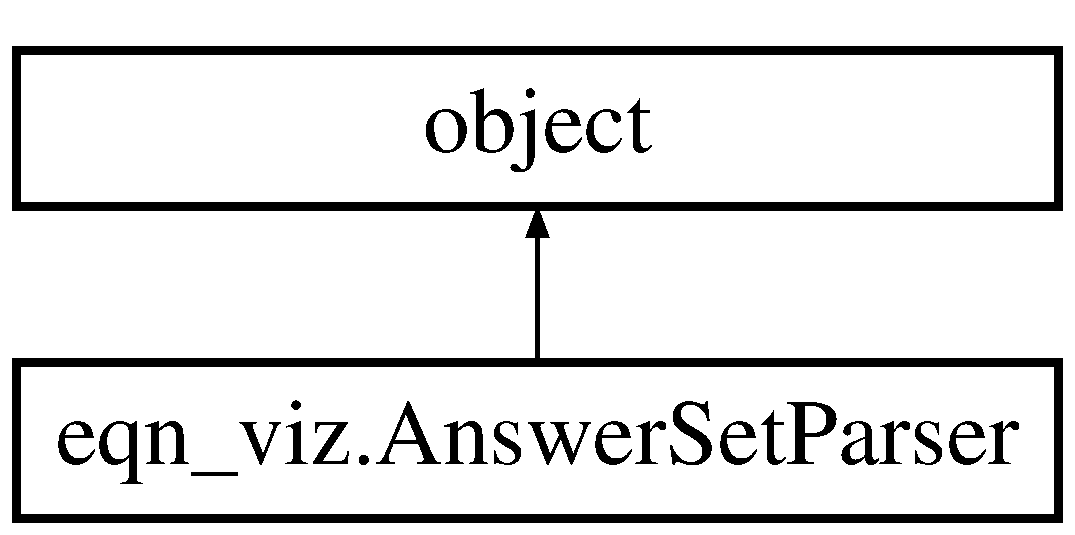
\includegraphics[height=2.000000cm]{classeqn__viz_1_1_answer_set_parser}
\end{center}
\end{figure}
\subsection*{Public Member Functions}
\begin{DoxyCompactItemize}
\item 
def \hyperlink{classeqn__viz_1_1_answer_set_parser_a250d2c845dbf332c9b1b1075eb357e99}{\+\_\+\+\_\+init\+\_\+\+\_\+} (self, predicates)
\item 
def \hyperlink{classeqn__viz_1_1_answer_set_parser_afa299b43fbe33fdefb8b2f2e33bac3a4}{parse\+Ans\+Set\+From\+Predicates} (self, predicates\+\_\+list)
\item 
def \hyperlink{classeqn__viz_1_1_answer_set_parser_a094b4e636447626a4f20cc12564758bf}{find\+Parser\+Matching\+Predicate}
\item 
def \hyperlink{classeqn__viz_1_1_answer_set_parser_a9133543e2c740202778d7cff12c7450c}{parse\+For\+Factor\+Predicates} (self, predicate)
\item 
def \hyperlink{classeqn__viz_1_1_answer_set_parser_ae3ed1620e24310cc4b448fd84d74c8a7}{get\+Math\+Problems} (self)
\item 
def \hyperlink{classeqn__viz_1_1_answer_set_parser_afebeba4a5dafaa167d0b7a2e76315a09}{get\+Generated\+Ans\+Set} (self)
\end{DoxyCompactItemize}
\subsection*{Public Attributes}
\begin{DoxyCompactItemize}
\item 
\hyperlink{classeqn__viz_1_1_answer_set_parser_aaf05269f220f98b07c9456d89ddca538}{math\+\_\+problems\+\_\+dict}
\end{DoxyCompactItemize}


\subsection{Detailed Description}


Definition at line 561 of file eqn\+\_\+viz.\+py.



\subsection{Constructor \& Destructor Documentation}
\hypertarget{classeqn__viz_1_1_answer_set_parser_a250d2c845dbf332c9b1b1075eb357e99}{}\index{eqn\+\_\+viz\+::\+Answer\+Set\+Parser@{eqn\+\_\+viz\+::\+Answer\+Set\+Parser}!\+\_\+\+\_\+init\+\_\+\+\_\+@{\+\_\+\+\_\+init\+\_\+\+\_\+}}
\index{\+\_\+\+\_\+init\+\_\+\+\_\+@{\+\_\+\+\_\+init\+\_\+\+\_\+}!eqn\+\_\+viz\+::\+Answer\+Set\+Parser@{eqn\+\_\+viz\+::\+Answer\+Set\+Parser}}
\subsubsection[{\+\_\+\+\_\+init\+\_\+\+\_\+}]{\setlength{\rightskip}{0pt plus 5cm}def eqn\+\_\+viz.\+Answer\+Set\+Parser.\+\_\+\+\_\+init\+\_\+\+\_\+ (
\begin{DoxyParamCaption}
\item[{}]{self, }
\item[{}]{predicates}
\end{DoxyParamCaption}
)}\label{classeqn__viz_1_1_answer_set_parser_a250d2c845dbf332c9b1b1075eb357e99}


Definition at line 562 of file eqn\+\_\+viz.\+py.



\subsection{Member Function Documentation}
\hypertarget{classeqn__viz_1_1_answer_set_parser_a094b4e636447626a4f20cc12564758bf}{}\index{eqn\+\_\+viz\+::\+Answer\+Set\+Parser@{eqn\+\_\+viz\+::\+Answer\+Set\+Parser}!find\+Parser\+Matching\+Predicate@{find\+Parser\+Matching\+Predicate}}
\index{find\+Parser\+Matching\+Predicate@{find\+Parser\+Matching\+Predicate}!eqn\+\_\+viz\+::\+Answer\+Set\+Parser@{eqn\+\_\+viz\+::\+Answer\+Set\+Parser}}
\subsubsection[{find\+Parser\+Matching\+Predicate}]{\setlength{\rightskip}{0pt plus 5cm}def eqn\+\_\+viz.\+Answer\+Set\+Parser.\+find\+Parser\+Matching\+Predicate (
\begin{DoxyParamCaption}
\item[{}]{self, }
\item[{}]{predicate, }
\item[{}]{parser\+\_\+list = {\ttfamily {\bf all\+\_\+parsers}}}
\end{DoxyParamCaption}
)}\label{classeqn__viz_1_1_answer_set_parser_a094b4e636447626a4f20cc12564758bf}
\begin{DoxyVerb}if any parser successfully parses the predicate, return tokens and the parser\end{DoxyVerb}
 

Definition at line 654 of file eqn\+\_\+viz.\+py.

\hypertarget{classeqn__viz_1_1_answer_set_parser_afebeba4a5dafaa167d0b7a2e76315a09}{}\index{eqn\+\_\+viz\+::\+Answer\+Set\+Parser@{eqn\+\_\+viz\+::\+Answer\+Set\+Parser}!get\+Generated\+Ans\+Set@{get\+Generated\+Ans\+Set}}
\index{get\+Generated\+Ans\+Set@{get\+Generated\+Ans\+Set}!eqn\+\_\+viz\+::\+Answer\+Set\+Parser@{eqn\+\_\+viz\+::\+Answer\+Set\+Parser}}
\subsubsection[{get\+Generated\+Ans\+Set}]{\setlength{\rightskip}{0pt plus 5cm}def eqn\+\_\+viz.\+Answer\+Set\+Parser.\+get\+Generated\+Ans\+Set (
\begin{DoxyParamCaption}
\item[{}]{self}
\end{DoxyParamCaption}
)}\label{classeqn__viz_1_1_answer_set_parser_afebeba4a5dafaa167d0b7a2e76315a09}


Definition at line 674 of file eqn\+\_\+viz.\+py.

\hypertarget{classeqn__viz_1_1_answer_set_parser_ae3ed1620e24310cc4b448fd84d74c8a7}{}\index{eqn\+\_\+viz\+::\+Answer\+Set\+Parser@{eqn\+\_\+viz\+::\+Answer\+Set\+Parser}!get\+Math\+Problems@{get\+Math\+Problems}}
\index{get\+Math\+Problems@{get\+Math\+Problems}!eqn\+\_\+viz\+::\+Answer\+Set\+Parser@{eqn\+\_\+viz\+::\+Answer\+Set\+Parser}}
\subsubsection[{get\+Math\+Problems}]{\setlength{\rightskip}{0pt plus 5cm}def eqn\+\_\+viz.\+Answer\+Set\+Parser.\+get\+Math\+Problems (
\begin{DoxyParamCaption}
\item[{}]{self}
\end{DoxyParamCaption}
)}\label{classeqn__viz_1_1_answer_set_parser_ae3ed1620e24310cc4b448fd84d74c8a7}


Definition at line 672 of file eqn\+\_\+viz.\+py.

\hypertarget{classeqn__viz_1_1_answer_set_parser_afa299b43fbe33fdefb8b2f2e33bac3a4}{}\index{eqn\+\_\+viz\+::\+Answer\+Set\+Parser@{eqn\+\_\+viz\+::\+Answer\+Set\+Parser}!parse\+Ans\+Set\+From\+Predicates@{parse\+Ans\+Set\+From\+Predicates}}
\index{parse\+Ans\+Set\+From\+Predicates@{parse\+Ans\+Set\+From\+Predicates}!eqn\+\_\+viz\+::\+Answer\+Set\+Parser@{eqn\+\_\+viz\+::\+Answer\+Set\+Parser}}
\subsubsection[{parse\+Ans\+Set\+From\+Predicates}]{\setlength{\rightskip}{0pt plus 5cm}def eqn\+\_\+viz.\+Answer\+Set\+Parser.\+parse\+Ans\+Set\+From\+Predicates (
\begin{DoxyParamCaption}
\item[{}]{self, }
\item[{}]{predicates\+\_\+list}
\end{DoxyParamCaption}
)}\label{classeqn__viz_1_1_answer_set_parser_afa299b43fbe33fdefb8b2f2e33bac3a4}
\begin{DoxyVerb}compose as a string every solution in the predicate list given\end{DoxyVerb}
 

Definition at line 565 of file eqn\+\_\+viz.\+py.

\hypertarget{classeqn__viz_1_1_answer_set_parser_a9133543e2c740202778d7cff12c7450c}{}\index{eqn\+\_\+viz\+::\+Answer\+Set\+Parser@{eqn\+\_\+viz\+::\+Answer\+Set\+Parser}!parse\+For\+Factor\+Predicates@{parse\+For\+Factor\+Predicates}}
\index{parse\+For\+Factor\+Predicates@{parse\+For\+Factor\+Predicates}!eqn\+\_\+viz\+::\+Answer\+Set\+Parser@{eqn\+\_\+viz\+::\+Answer\+Set\+Parser}}
\subsubsection[{parse\+For\+Factor\+Predicates}]{\setlength{\rightskip}{0pt plus 5cm}def eqn\+\_\+viz.\+Answer\+Set\+Parser.\+parse\+For\+Factor\+Predicates (
\begin{DoxyParamCaption}
\item[{}]{self, }
\item[{}]{predicate}
\end{DoxyParamCaption}
)}\label{classeqn__viz_1_1_answer_set_parser_a9133543e2c740202778d7cff12c7450c}
\begin{DoxyVerb}if any parser successfully parses the predicate, return tokens and the parser\end{DoxyVerb}
 

Definition at line 663 of file eqn\+\_\+viz.\+py.



\subsection{Member Data Documentation}
\hypertarget{classeqn__viz_1_1_answer_set_parser_aaf05269f220f98b07c9456d89ddca538}{}\index{eqn\+\_\+viz\+::\+Answer\+Set\+Parser@{eqn\+\_\+viz\+::\+Answer\+Set\+Parser}!math\+\_\+problems\+\_\+dict@{math\+\_\+problems\+\_\+dict}}
\index{math\+\_\+problems\+\_\+dict@{math\+\_\+problems\+\_\+dict}!eqn\+\_\+viz\+::\+Answer\+Set\+Parser@{eqn\+\_\+viz\+::\+Answer\+Set\+Parser}}
\subsubsection[{math\+\_\+problems\+\_\+dict}]{\setlength{\rightskip}{0pt plus 5cm}eqn\+\_\+viz.\+Answer\+Set\+Parser.\+math\+\_\+problems\+\_\+dict}\label{classeqn__viz_1_1_answer_set_parser_aaf05269f220f98b07c9456d89ddca538}


Definition at line 563 of file eqn\+\_\+viz.\+py.



The documentation for this class was generated from the following file\+:\begin{DoxyCompactItemize}
\item 
\hyperlink{eqn__viz_8py}{eqn\+\_\+viz.\+py}\end{DoxyCompactItemize}

\hypertarget{class_prolog_rules_parser_1_1_prolog_rules_parser_1_1_args_context}{}\section{Prolog\+Rules\+Parser.\+Prolog\+Rules\+Parser.\+Args\+Context Class Reference}
\label{class_prolog_rules_parser_1_1_prolog_rules_parser_1_1_args_context}\index{Prolog\+Rules\+Parser.\+Prolog\+Rules\+Parser.\+Args\+Context@{Prolog\+Rules\+Parser.\+Prolog\+Rules\+Parser.\+Args\+Context}}
Inheritance diagram for Prolog\+Rules\+Parser.\+Prolog\+Rules\+Parser.\+Args\+Context\+:\begin{figure}[H]
\begin{center}
\leavevmode
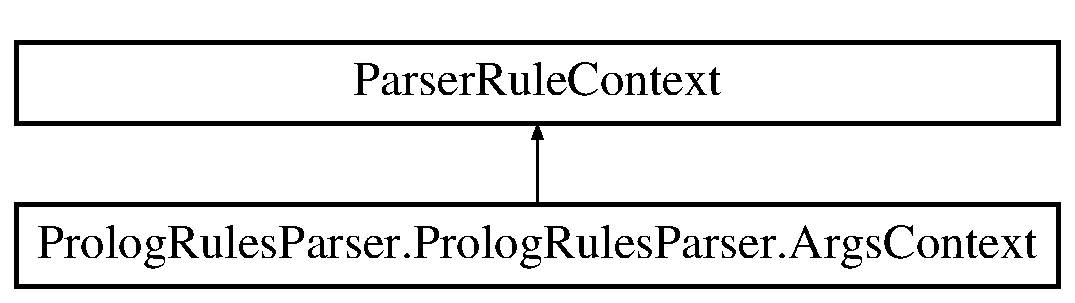
\includegraphics[height=2.000000cm]{class_prolog_rules_parser_1_1_prolog_rules_parser_1_1_args_context}
\end{center}
\end{figure}
\subsection*{Public Member Functions}
\begin{DoxyCompactItemize}
\item 
def \hyperlink{class_prolog_rules_parser_1_1_prolog_rules_parser_1_1_args_context_a92922f84a340c490b424581280adc314}{\+\_\+\+\_\+init\+\_\+\+\_\+}
\item 
def \hyperlink{class_prolog_rules_parser_1_1_prolog_rules_parser_1_1_args_context_acf6c63aed1cdaf0db3191d2ba1350bca}{onearg}
\item 
def \hyperlink{class_prolog_rules_parser_1_1_prolog_rules_parser_1_1_args_context_a2a9420b4abb263666018a5dc664476b3}{get\+Rule\+Index} (self)
\item 
def \hyperlink{class_prolog_rules_parser_1_1_prolog_rules_parser_1_1_args_context_a4a980aace602a76508d43a6aabdd927c}{enter\+Rule} (self, listener)
\item 
def \hyperlink{class_prolog_rules_parser_1_1_prolog_rules_parser_1_1_args_context_abad9fd1b2685f5e8002537178b1bde68}{exit\+Rule} (self, listener)
\end{DoxyCompactItemize}
\subsection*{Public Attributes}
\begin{DoxyCompactItemize}
\item 
\hyperlink{class_prolog_rules_parser_1_1_prolog_rules_parser_1_1_args_context_ad3fbe43f28dfe195ab66b4bb598a7a46}{parser}
\end{DoxyCompactItemize}


\subsection{Detailed Description}


Definition at line 985 of file Prolog\+Rules\+Parser.\+py.



\subsection{Constructor \& Destructor Documentation}
\hypertarget{class_prolog_rules_parser_1_1_prolog_rules_parser_1_1_args_context_a92922f84a340c490b424581280adc314}{}\index{Prolog\+Rules\+Parser\+::\+Prolog\+Rules\+Parser\+::\+Args\+Context@{Prolog\+Rules\+Parser\+::\+Prolog\+Rules\+Parser\+::\+Args\+Context}!\+\_\+\+\_\+init\+\_\+\+\_\+@{\+\_\+\+\_\+init\+\_\+\+\_\+}}
\index{\+\_\+\+\_\+init\+\_\+\+\_\+@{\+\_\+\+\_\+init\+\_\+\+\_\+}!Prolog\+Rules\+Parser\+::\+Prolog\+Rules\+Parser\+::\+Args\+Context@{Prolog\+Rules\+Parser\+::\+Prolog\+Rules\+Parser\+::\+Args\+Context}}
\subsubsection[{\+\_\+\+\_\+init\+\_\+\+\_\+}]{\setlength{\rightskip}{0pt plus 5cm}def Prolog\+Rules\+Parser.\+Prolog\+Rules\+Parser.\+Args\+Context.\+\_\+\+\_\+init\+\_\+\+\_\+ (
\begin{DoxyParamCaption}
\item[{}]{self, }
\item[{}]{parser, }
\item[{}]{parent = {\ttfamily None}, }
\item[{}]{invoking\+State = {\ttfamily -\/1}}
\end{DoxyParamCaption}
)}\label{class_prolog_rules_parser_1_1_prolog_rules_parser_1_1_args_context_a92922f84a340c490b424581280adc314}


Definition at line 987 of file Prolog\+Rules\+Parser.\+py.



\subsection{Member Function Documentation}
\hypertarget{class_prolog_rules_parser_1_1_prolog_rules_parser_1_1_args_context_a4a980aace602a76508d43a6aabdd927c}{}\index{Prolog\+Rules\+Parser\+::\+Prolog\+Rules\+Parser\+::\+Args\+Context@{Prolog\+Rules\+Parser\+::\+Prolog\+Rules\+Parser\+::\+Args\+Context}!enter\+Rule@{enter\+Rule}}
\index{enter\+Rule@{enter\+Rule}!Prolog\+Rules\+Parser\+::\+Prolog\+Rules\+Parser\+::\+Args\+Context@{Prolog\+Rules\+Parser\+::\+Prolog\+Rules\+Parser\+::\+Args\+Context}}
\subsubsection[{enter\+Rule}]{\setlength{\rightskip}{0pt plus 5cm}def Prolog\+Rules\+Parser.\+Prolog\+Rules\+Parser.\+Args\+Context.\+enter\+Rule (
\begin{DoxyParamCaption}
\item[{}]{self, }
\item[{}]{listener}
\end{DoxyParamCaption}
)}\label{class_prolog_rules_parser_1_1_prolog_rules_parser_1_1_args_context_a4a980aace602a76508d43a6aabdd927c}


Definition at line 1001 of file Prolog\+Rules\+Parser.\+py.

\hypertarget{class_prolog_rules_parser_1_1_prolog_rules_parser_1_1_args_context_abad9fd1b2685f5e8002537178b1bde68}{}\index{Prolog\+Rules\+Parser\+::\+Prolog\+Rules\+Parser\+::\+Args\+Context@{Prolog\+Rules\+Parser\+::\+Prolog\+Rules\+Parser\+::\+Args\+Context}!exit\+Rule@{exit\+Rule}}
\index{exit\+Rule@{exit\+Rule}!Prolog\+Rules\+Parser\+::\+Prolog\+Rules\+Parser\+::\+Args\+Context@{Prolog\+Rules\+Parser\+::\+Prolog\+Rules\+Parser\+::\+Args\+Context}}
\subsubsection[{exit\+Rule}]{\setlength{\rightskip}{0pt plus 5cm}def Prolog\+Rules\+Parser.\+Prolog\+Rules\+Parser.\+Args\+Context.\+exit\+Rule (
\begin{DoxyParamCaption}
\item[{}]{self, }
\item[{}]{listener}
\end{DoxyParamCaption}
)}\label{class_prolog_rules_parser_1_1_prolog_rules_parser_1_1_args_context_abad9fd1b2685f5e8002537178b1bde68}


Definition at line 1005 of file Prolog\+Rules\+Parser.\+py.

\hypertarget{class_prolog_rules_parser_1_1_prolog_rules_parser_1_1_args_context_a2a9420b4abb263666018a5dc664476b3}{}\index{Prolog\+Rules\+Parser\+::\+Prolog\+Rules\+Parser\+::\+Args\+Context@{Prolog\+Rules\+Parser\+::\+Prolog\+Rules\+Parser\+::\+Args\+Context}!get\+Rule\+Index@{get\+Rule\+Index}}
\index{get\+Rule\+Index@{get\+Rule\+Index}!Prolog\+Rules\+Parser\+::\+Prolog\+Rules\+Parser\+::\+Args\+Context@{Prolog\+Rules\+Parser\+::\+Prolog\+Rules\+Parser\+::\+Args\+Context}}
\subsubsection[{get\+Rule\+Index}]{\setlength{\rightskip}{0pt plus 5cm}def Prolog\+Rules\+Parser.\+Prolog\+Rules\+Parser.\+Args\+Context.\+get\+Rule\+Index (
\begin{DoxyParamCaption}
\item[{}]{self}
\end{DoxyParamCaption}
)}\label{class_prolog_rules_parser_1_1_prolog_rules_parser_1_1_args_context_a2a9420b4abb263666018a5dc664476b3}


Definition at line 998 of file Prolog\+Rules\+Parser.\+py.

\hypertarget{class_prolog_rules_parser_1_1_prolog_rules_parser_1_1_args_context_acf6c63aed1cdaf0db3191d2ba1350bca}{}\index{Prolog\+Rules\+Parser\+::\+Prolog\+Rules\+Parser\+::\+Args\+Context@{Prolog\+Rules\+Parser\+::\+Prolog\+Rules\+Parser\+::\+Args\+Context}!onearg@{onearg}}
\index{onearg@{onearg}!Prolog\+Rules\+Parser\+::\+Prolog\+Rules\+Parser\+::\+Args\+Context@{Prolog\+Rules\+Parser\+::\+Prolog\+Rules\+Parser\+::\+Args\+Context}}
\subsubsection[{onearg}]{\setlength{\rightskip}{0pt plus 5cm}def Prolog\+Rules\+Parser.\+Prolog\+Rules\+Parser.\+Args\+Context.\+onearg (
\begin{DoxyParamCaption}
\item[{}]{self, }
\item[{}]{i = {\ttfamily None}}
\end{DoxyParamCaption}
)}\label{class_prolog_rules_parser_1_1_prolog_rules_parser_1_1_args_context_acf6c63aed1cdaf0db3191d2ba1350bca}


Definition at line 991 of file Prolog\+Rules\+Parser.\+py.



\subsection{Member Data Documentation}
\hypertarget{class_prolog_rules_parser_1_1_prolog_rules_parser_1_1_args_context_ad3fbe43f28dfe195ab66b4bb598a7a46}{}\index{Prolog\+Rules\+Parser\+::\+Prolog\+Rules\+Parser\+::\+Args\+Context@{Prolog\+Rules\+Parser\+::\+Prolog\+Rules\+Parser\+::\+Args\+Context}!parser@{parser}}
\index{parser@{parser}!Prolog\+Rules\+Parser\+::\+Prolog\+Rules\+Parser\+::\+Args\+Context@{Prolog\+Rules\+Parser\+::\+Prolog\+Rules\+Parser\+::\+Args\+Context}}
\subsubsection[{parser}]{\setlength{\rightskip}{0pt plus 5cm}Prolog\+Rules\+Parser.\+Prolog\+Rules\+Parser.\+Args\+Context.\+parser}\label{class_prolog_rules_parser_1_1_prolog_rules_parser_1_1_args_context_ad3fbe43f28dfe195ab66b4bb598a7a46}


Definition at line 989 of file Prolog\+Rules\+Parser.\+py.



The documentation for this class was generated from the following file\+:\begin{DoxyCompactItemize}
\item 
\hyperlink{_prolog_rules_parser_8py}{Prolog\+Rules\+Parser.\+py}\end{DoxyCompactItemize}

\hypertarget{class_prolog_rules_parser_1_1_prolog_rules_parser_1_1_atom_context}{}\section{Prolog\+Rules\+Parser.\+Prolog\+Rules\+Parser.\+Atom\+Context Class Reference}
\label{class_prolog_rules_parser_1_1_prolog_rules_parser_1_1_atom_context}\index{Prolog\+Rules\+Parser.\+Prolog\+Rules\+Parser.\+Atom\+Context@{Prolog\+Rules\+Parser.\+Prolog\+Rules\+Parser.\+Atom\+Context}}
Inheritance diagram for Prolog\+Rules\+Parser.\+Prolog\+Rules\+Parser.\+Atom\+Context\+:\begin{figure}[H]
\begin{center}
\leavevmode
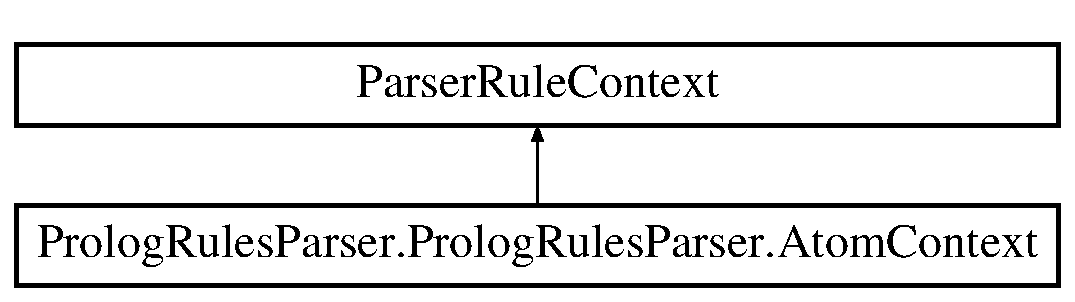
\includegraphics[height=2.000000cm]{class_prolog_rules_parser_1_1_prolog_rules_parser_1_1_atom_context}
\end{center}
\end{figure}
\subsection*{Public Member Functions}
\begin{DoxyCompactItemize}
\item 
def \hyperlink{class_prolog_rules_parser_1_1_prolog_rules_parser_1_1_atom_context_ade2e61ecb9a528e958814fb70d76a4b8}{\+\_\+\+\_\+init\+\_\+\+\_\+}
\item 
def \hyperlink{class_prolog_rules_parser_1_1_prolog_rules_parser_1_1_atom_context_a4eea8ead093ada75092e215728604b31}{N\+U\+M\+B\+E\+R} (self)
\item 
def \hyperlink{class_prolog_rules_parser_1_1_prolog_rules_parser_1_1_atom_context_a9166f9e79a4a3a62d4465407c375a52a}{identifier} (self)
\item 
def \hyperlink{class_prolog_rules_parser_1_1_prolog_rules_parser_1_1_atom_context_a6fbdeee4afaad7b66848f7be5e97dd58}{get\+Rule\+Index} (self)
\item 
def \hyperlink{class_prolog_rules_parser_1_1_prolog_rules_parser_1_1_atom_context_ab5403293233289dd5274f3233fd497d3}{enter\+Rule} (self, listener)
\item 
def \hyperlink{class_prolog_rules_parser_1_1_prolog_rules_parser_1_1_atom_context_a2ed6f6b49de2a40c4a316cb0a7d11b1f}{exit\+Rule} (self, listener)
\end{DoxyCompactItemize}
\subsection*{Public Attributes}
\begin{DoxyCompactItemize}
\item 
\hyperlink{class_prolog_rules_parser_1_1_prolog_rules_parser_1_1_atom_context_a17b3a62241e244ba246e624a57564a51}{parser}
\end{DoxyCompactItemize}


\subsection{Detailed Description}


Definition at line 1097 of file Prolog\+Rules\+Parser.\+py.



\subsection{Constructor \& Destructor Documentation}
\hypertarget{class_prolog_rules_parser_1_1_prolog_rules_parser_1_1_atom_context_ade2e61ecb9a528e958814fb70d76a4b8}{}\index{Prolog\+Rules\+Parser\+::\+Prolog\+Rules\+Parser\+::\+Atom\+Context@{Prolog\+Rules\+Parser\+::\+Prolog\+Rules\+Parser\+::\+Atom\+Context}!\+\_\+\+\_\+init\+\_\+\+\_\+@{\+\_\+\+\_\+init\+\_\+\+\_\+}}
\index{\+\_\+\+\_\+init\+\_\+\+\_\+@{\+\_\+\+\_\+init\+\_\+\+\_\+}!Prolog\+Rules\+Parser\+::\+Prolog\+Rules\+Parser\+::\+Atom\+Context@{Prolog\+Rules\+Parser\+::\+Prolog\+Rules\+Parser\+::\+Atom\+Context}}
\subsubsection[{\+\_\+\+\_\+init\+\_\+\+\_\+}]{\setlength{\rightskip}{0pt plus 5cm}def Prolog\+Rules\+Parser.\+Prolog\+Rules\+Parser.\+Atom\+Context.\+\_\+\+\_\+init\+\_\+\+\_\+ (
\begin{DoxyParamCaption}
\item[{}]{self, }
\item[{}]{parser, }
\item[{}]{parent = {\ttfamily None}, }
\item[{}]{invoking\+State = {\ttfamily -\/1}}
\end{DoxyParamCaption}
)}\label{class_prolog_rules_parser_1_1_prolog_rules_parser_1_1_atom_context_ade2e61ecb9a528e958814fb70d76a4b8}


Definition at line 1099 of file Prolog\+Rules\+Parser.\+py.



\subsection{Member Function Documentation}
\hypertarget{class_prolog_rules_parser_1_1_prolog_rules_parser_1_1_atom_context_ab5403293233289dd5274f3233fd497d3}{}\index{Prolog\+Rules\+Parser\+::\+Prolog\+Rules\+Parser\+::\+Atom\+Context@{Prolog\+Rules\+Parser\+::\+Prolog\+Rules\+Parser\+::\+Atom\+Context}!enter\+Rule@{enter\+Rule}}
\index{enter\+Rule@{enter\+Rule}!Prolog\+Rules\+Parser\+::\+Prolog\+Rules\+Parser\+::\+Atom\+Context@{Prolog\+Rules\+Parser\+::\+Prolog\+Rules\+Parser\+::\+Atom\+Context}}
\subsubsection[{enter\+Rule}]{\setlength{\rightskip}{0pt plus 5cm}def Prolog\+Rules\+Parser.\+Prolog\+Rules\+Parser.\+Atom\+Context.\+enter\+Rule (
\begin{DoxyParamCaption}
\item[{}]{self, }
\item[{}]{listener}
\end{DoxyParamCaption}
)}\label{class_prolog_rules_parser_1_1_prolog_rules_parser_1_1_atom_context_ab5403293233289dd5274f3233fd497d3}


Definition at line 1113 of file Prolog\+Rules\+Parser.\+py.

\hypertarget{class_prolog_rules_parser_1_1_prolog_rules_parser_1_1_atom_context_a2ed6f6b49de2a40c4a316cb0a7d11b1f}{}\index{Prolog\+Rules\+Parser\+::\+Prolog\+Rules\+Parser\+::\+Atom\+Context@{Prolog\+Rules\+Parser\+::\+Prolog\+Rules\+Parser\+::\+Atom\+Context}!exit\+Rule@{exit\+Rule}}
\index{exit\+Rule@{exit\+Rule}!Prolog\+Rules\+Parser\+::\+Prolog\+Rules\+Parser\+::\+Atom\+Context@{Prolog\+Rules\+Parser\+::\+Prolog\+Rules\+Parser\+::\+Atom\+Context}}
\subsubsection[{exit\+Rule}]{\setlength{\rightskip}{0pt plus 5cm}def Prolog\+Rules\+Parser.\+Prolog\+Rules\+Parser.\+Atom\+Context.\+exit\+Rule (
\begin{DoxyParamCaption}
\item[{}]{self, }
\item[{}]{listener}
\end{DoxyParamCaption}
)}\label{class_prolog_rules_parser_1_1_prolog_rules_parser_1_1_atom_context_a2ed6f6b49de2a40c4a316cb0a7d11b1f}


Definition at line 1117 of file Prolog\+Rules\+Parser.\+py.

\hypertarget{class_prolog_rules_parser_1_1_prolog_rules_parser_1_1_atom_context_a6fbdeee4afaad7b66848f7be5e97dd58}{}\index{Prolog\+Rules\+Parser\+::\+Prolog\+Rules\+Parser\+::\+Atom\+Context@{Prolog\+Rules\+Parser\+::\+Prolog\+Rules\+Parser\+::\+Atom\+Context}!get\+Rule\+Index@{get\+Rule\+Index}}
\index{get\+Rule\+Index@{get\+Rule\+Index}!Prolog\+Rules\+Parser\+::\+Prolog\+Rules\+Parser\+::\+Atom\+Context@{Prolog\+Rules\+Parser\+::\+Prolog\+Rules\+Parser\+::\+Atom\+Context}}
\subsubsection[{get\+Rule\+Index}]{\setlength{\rightskip}{0pt plus 5cm}def Prolog\+Rules\+Parser.\+Prolog\+Rules\+Parser.\+Atom\+Context.\+get\+Rule\+Index (
\begin{DoxyParamCaption}
\item[{}]{self}
\end{DoxyParamCaption}
)}\label{class_prolog_rules_parser_1_1_prolog_rules_parser_1_1_atom_context_a6fbdeee4afaad7b66848f7be5e97dd58}


Definition at line 1110 of file Prolog\+Rules\+Parser.\+py.

\hypertarget{class_prolog_rules_parser_1_1_prolog_rules_parser_1_1_atom_context_a9166f9e79a4a3a62d4465407c375a52a}{}\index{Prolog\+Rules\+Parser\+::\+Prolog\+Rules\+Parser\+::\+Atom\+Context@{Prolog\+Rules\+Parser\+::\+Prolog\+Rules\+Parser\+::\+Atom\+Context}!identifier@{identifier}}
\index{identifier@{identifier}!Prolog\+Rules\+Parser\+::\+Prolog\+Rules\+Parser\+::\+Atom\+Context@{Prolog\+Rules\+Parser\+::\+Prolog\+Rules\+Parser\+::\+Atom\+Context}}
\subsubsection[{identifier}]{\setlength{\rightskip}{0pt plus 5cm}def Prolog\+Rules\+Parser.\+Prolog\+Rules\+Parser.\+Atom\+Context.\+identifier (
\begin{DoxyParamCaption}
\item[{}]{self}
\end{DoxyParamCaption}
)}\label{class_prolog_rules_parser_1_1_prolog_rules_parser_1_1_atom_context_a9166f9e79a4a3a62d4465407c375a52a}


Definition at line 1106 of file Prolog\+Rules\+Parser.\+py.

\hypertarget{class_prolog_rules_parser_1_1_prolog_rules_parser_1_1_atom_context_a4eea8ead093ada75092e215728604b31}{}\index{Prolog\+Rules\+Parser\+::\+Prolog\+Rules\+Parser\+::\+Atom\+Context@{Prolog\+Rules\+Parser\+::\+Prolog\+Rules\+Parser\+::\+Atom\+Context}!N\+U\+M\+B\+E\+R@{N\+U\+M\+B\+E\+R}}
\index{N\+U\+M\+B\+E\+R@{N\+U\+M\+B\+E\+R}!Prolog\+Rules\+Parser\+::\+Prolog\+Rules\+Parser\+::\+Atom\+Context@{Prolog\+Rules\+Parser\+::\+Prolog\+Rules\+Parser\+::\+Atom\+Context}}
\subsubsection[{N\+U\+M\+B\+E\+R}]{\setlength{\rightskip}{0pt plus 5cm}def Prolog\+Rules\+Parser.\+Prolog\+Rules\+Parser.\+Atom\+Context.\+N\+U\+M\+B\+E\+R (
\begin{DoxyParamCaption}
\item[{}]{self}
\end{DoxyParamCaption}
)}\label{class_prolog_rules_parser_1_1_prolog_rules_parser_1_1_atom_context_a4eea8ead093ada75092e215728604b31}


Definition at line 1103 of file Prolog\+Rules\+Parser.\+py.



\subsection{Member Data Documentation}
\hypertarget{class_prolog_rules_parser_1_1_prolog_rules_parser_1_1_atom_context_a17b3a62241e244ba246e624a57564a51}{}\index{Prolog\+Rules\+Parser\+::\+Prolog\+Rules\+Parser\+::\+Atom\+Context@{Prolog\+Rules\+Parser\+::\+Prolog\+Rules\+Parser\+::\+Atom\+Context}!parser@{parser}}
\index{parser@{parser}!Prolog\+Rules\+Parser\+::\+Prolog\+Rules\+Parser\+::\+Atom\+Context@{Prolog\+Rules\+Parser\+::\+Prolog\+Rules\+Parser\+::\+Atom\+Context}}
\subsubsection[{parser}]{\setlength{\rightskip}{0pt plus 5cm}Prolog\+Rules\+Parser.\+Prolog\+Rules\+Parser.\+Atom\+Context.\+parser}\label{class_prolog_rules_parser_1_1_prolog_rules_parser_1_1_atom_context_a17b3a62241e244ba246e624a57564a51}


Definition at line 1101 of file Prolog\+Rules\+Parser.\+py.



The documentation for this class was generated from the following file\+:\begin{DoxyCompactItemize}
\item 
\hyperlink{_prolog_rules_parser_8py}{Prolog\+Rules\+Parser.\+py}\end{DoxyCompactItemize}

\hypertarget{class_prolog_rules_parser_1_1_prolog_rules_parser_1_1_comparator_context}{}\section{Prolog\+Rules\+Parser.\+Prolog\+Rules\+Parser.\+Comparator\+Context Class Reference}
\label{class_prolog_rules_parser_1_1_prolog_rules_parser_1_1_comparator_context}\index{Prolog\+Rules\+Parser.\+Prolog\+Rules\+Parser.\+Comparator\+Context@{Prolog\+Rules\+Parser.\+Prolog\+Rules\+Parser.\+Comparator\+Context}}
Inheritance diagram for Prolog\+Rules\+Parser.\+Prolog\+Rules\+Parser.\+Comparator\+Context\+:\begin{figure}[H]
\begin{center}
\leavevmode
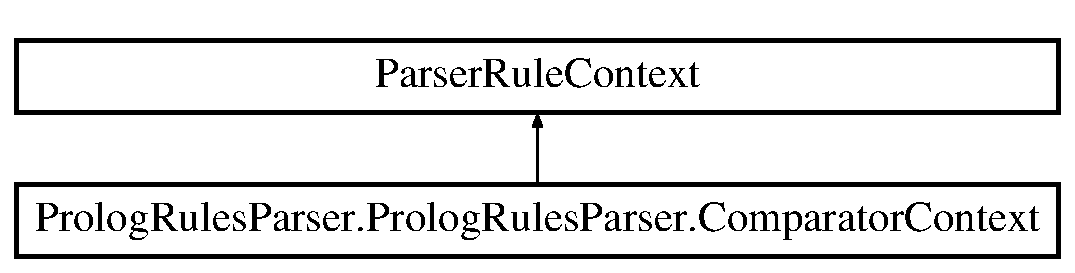
\includegraphics[height=2.000000cm]{class_prolog_rules_parser_1_1_prolog_rules_parser_1_1_comparator_context}
\end{center}
\end{figure}
\subsection*{Public Member Functions}
\begin{DoxyCompactItemize}
\item 
def \hyperlink{class_prolog_rules_parser_1_1_prolog_rules_parser_1_1_comparator_context_a3fa1e3f0a849de47ff9c6cd4d3e62cc7}{\+\_\+\+\_\+init\+\_\+\+\_\+}
\item 
def \hyperlink{class_prolog_rules_parser_1_1_prolog_rules_parser_1_1_comparator_context_aac147d40792d5173f0d6581574929f5d}{mathexpr} (self)
\item 
def \hyperlink{class_prolog_rules_parser_1_1_prolog_rules_parser_1_1_comparator_context_ac1077a09906c3e53c18b6ca48db5b435}{R\+E\+L\+O\+P\+E\+R\+A\+T\+O\+R} (self)
\item 
def \hyperlink{class_prolog_rules_parser_1_1_prolog_rules_parser_1_1_comparator_context_a4632d209ecd5ff9e15d9941feab6f521}{atom} (self)
\item 
def \hyperlink{class_prolog_rules_parser_1_1_prolog_rules_parser_1_1_comparator_context_a21d1fa2b566f2f56dda09564a4091a75}{get\+Rule\+Index} (self)
\item 
def \hyperlink{class_prolog_rules_parser_1_1_prolog_rules_parser_1_1_comparator_context_ab3a7b87f4021da092f1102b1e89e6ced}{enter\+Rule} (self, listener)
\item 
def \hyperlink{class_prolog_rules_parser_1_1_prolog_rules_parser_1_1_comparator_context_aa3db6669684f178ae22e86b64422f960}{exit\+Rule} (self, listener)
\end{DoxyCompactItemize}
\subsection*{Public Attributes}
\begin{DoxyCompactItemize}
\item 
\hyperlink{class_prolog_rules_parser_1_1_prolog_rules_parser_1_1_comparator_context_ac4400f4e8f1a4122592bfc45e9902bc2}{parser}
\end{DoxyCompactItemize}


\subsection{Detailed Description}


Definition at line 853 of file Prolog\+Rules\+Parser.\+py.



\subsection{Constructor \& Destructor Documentation}
\hypertarget{class_prolog_rules_parser_1_1_prolog_rules_parser_1_1_comparator_context_a3fa1e3f0a849de47ff9c6cd4d3e62cc7}{}\index{Prolog\+Rules\+Parser\+::\+Prolog\+Rules\+Parser\+::\+Comparator\+Context@{Prolog\+Rules\+Parser\+::\+Prolog\+Rules\+Parser\+::\+Comparator\+Context}!\+\_\+\+\_\+init\+\_\+\+\_\+@{\+\_\+\+\_\+init\+\_\+\+\_\+}}
\index{\+\_\+\+\_\+init\+\_\+\+\_\+@{\+\_\+\+\_\+init\+\_\+\+\_\+}!Prolog\+Rules\+Parser\+::\+Prolog\+Rules\+Parser\+::\+Comparator\+Context@{Prolog\+Rules\+Parser\+::\+Prolog\+Rules\+Parser\+::\+Comparator\+Context}}
\subsubsection[{\+\_\+\+\_\+init\+\_\+\+\_\+}]{\setlength{\rightskip}{0pt plus 5cm}def Prolog\+Rules\+Parser.\+Prolog\+Rules\+Parser.\+Comparator\+Context.\+\_\+\+\_\+init\+\_\+\+\_\+ (
\begin{DoxyParamCaption}
\item[{}]{self, }
\item[{}]{parser, }
\item[{}]{parent = {\ttfamily None}, }
\item[{}]{invoking\+State = {\ttfamily -\/1}}
\end{DoxyParamCaption}
)}\label{class_prolog_rules_parser_1_1_prolog_rules_parser_1_1_comparator_context_a3fa1e3f0a849de47ff9c6cd4d3e62cc7}


Definition at line 855 of file Prolog\+Rules\+Parser.\+py.



\subsection{Member Function Documentation}
\hypertarget{class_prolog_rules_parser_1_1_prolog_rules_parser_1_1_comparator_context_a4632d209ecd5ff9e15d9941feab6f521}{}\index{Prolog\+Rules\+Parser\+::\+Prolog\+Rules\+Parser\+::\+Comparator\+Context@{Prolog\+Rules\+Parser\+::\+Prolog\+Rules\+Parser\+::\+Comparator\+Context}!atom@{atom}}
\index{atom@{atom}!Prolog\+Rules\+Parser\+::\+Prolog\+Rules\+Parser\+::\+Comparator\+Context@{Prolog\+Rules\+Parser\+::\+Prolog\+Rules\+Parser\+::\+Comparator\+Context}}
\subsubsection[{atom}]{\setlength{\rightskip}{0pt plus 5cm}def Prolog\+Rules\+Parser.\+Prolog\+Rules\+Parser.\+Comparator\+Context.\+atom (
\begin{DoxyParamCaption}
\item[{}]{self}
\end{DoxyParamCaption}
)}\label{class_prolog_rules_parser_1_1_prolog_rules_parser_1_1_comparator_context_a4632d209ecd5ff9e15d9941feab6f521}


Definition at line 866 of file Prolog\+Rules\+Parser.\+py.

\hypertarget{class_prolog_rules_parser_1_1_prolog_rules_parser_1_1_comparator_context_ab3a7b87f4021da092f1102b1e89e6ced}{}\index{Prolog\+Rules\+Parser\+::\+Prolog\+Rules\+Parser\+::\+Comparator\+Context@{Prolog\+Rules\+Parser\+::\+Prolog\+Rules\+Parser\+::\+Comparator\+Context}!enter\+Rule@{enter\+Rule}}
\index{enter\+Rule@{enter\+Rule}!Prolog\+Rules\+Parser\+::\+Prolog\+Rules\+Parser\+::\+Comparator\+Context@{Prolog\+Rules\+Parser\+::\+Prolog\+Rules\+Parser\+::\+Comparator\+Context}}
\subsubsection[{enter\+Rule}]{\setlength{\rightskip}{0pt plus 5cm}def Prolog\+Rules\+Parser.\+Prolog\+Rules\+Parser.\+Comparator\+Context.\+enter\+Rule (
\begin{DoxyParamCaption}
\item[{}]{self, }
\item[{}]{listener}
\end{DoxyParamCaption}
)}\label{class_prolog_rules_parser_1_1_prolog_rules_parser_1_1_comparator_context_ab3a7b87f4021da092f1102b1e89e6ced}


Definition at line 873 of file Prolog\+Rules\+Parser.\+py.

\hypertarget{class_prolog_rules_parser_1_1_prolog_rules_parser_1_1_comparator_context_aa3db6669684f178ae22e86b64422f960}{}\index{Prolog\+Rules\+Parser\+::\+Prolog\+Rules\+Parser\+::\+Comparator\+Context@{Prolog\+Rules\+Parser\+::\+Prolog\+Rules\+Parser\+::\+Comparator\+Context}!exit\+Rule@{exit\+Rule}}
\index{exit\+Rule@{exit\+Rule}!Prolog\+Rules\+Parser\+::\+Prolog\+Rules\+Parser\+::\+Comparator\+Context@{Prolog\+Rules\+Parser\+::\+Prolog\+Rules\+Parser\+::\+Comparator\+Context}}
\subsubsection[{exit\+Rule}]{\setlength{\rightskip}{0pt plus 5cm}def Prolog\+Rules\+Parser.\+Prolog\+Rules\+Parser.\+Comparator\+Context.\+exit\+Rule (
\begin{DoxyParamCaption}
\item[{}]{self, }
\item[{}]{listener}
\end{DoxyParamCaption}
)}\label{class_prolog_rules_parser_1_1_prolog_rules_parser_1_1_comparator_context_aa3db6669684f178ae22e86b64422f960}


Definition at line 877 of file Prolog\+Rules\+Parser.\+py.

\hypertarget{class_prolog_rules_parser_1_1_prolog_rules_parser_1_1_comparator_context_a21d1fa2b566f2f56dda09564a4091a75}{}\index{Prolog\+Rules\+Parser\+::\+Prolog\+Rules\+Parser\+::\+Comparator\+Context@{Prolog\+Rules\+Parser\+::\+Prolog\+Rules\+Parser\+::\+Comparator\+Context}!get\+Rule\+Index@{get\+Rule\+Index}}
\index{get\+Rule\+Index@{get\+Rule\+Index}!Prolog\+Rules\+Parser\+::\+Prolog\+Rules\+Parser\+::\+Comparator\+Context@{Prolog\+Rules\+Parser\+::\+Prolog\+Rules\+Parser\+::\+Comparator\+Context}}
\subsubsection[{get\+Rule\+Index}]{\setlength{\rightskip}{0pt plus 5cm}def Prolog\+Rules\+Parser.\+Prolog\+Rules\+Parser.\+Comparator\+Context.\+get\+Rule\+Index (
\begin{DoxyParamCaption}
\item[{}]{self}
\end{DoxyParamCaption}
)}\label{class_prolog_rules_parser_1_1_prolog_rules_parser_1_1_comparator_context_a21d1fa2b566f2f56dda09564a4091a75}


Definition at line 870 of file Prolog\+Rules\+Parser.\+py.

\hypertarget{class_prolog_rules_parser_1_1_prolog_rules_parser_1_1_comparator_context_aac147d40792d5173f0d6581574929f5d}{}\index{Prolog\+Rules\+Parser\+::\+Prolog\+Rules\+Parser\+::\+Comparator\+Context@{Prolog\+Rules\+Parser\+::\+Prolog\+Rules\+Parser\+::\+Comparator\+Context}!mathexpr@{mathexpr}}
\index{mathexpr@{mathexpr}!Prolog\+Rules\+Parser\+::\+Prolog\+Rules\+Parser\+::\+Comparator\+Context@{Prolog\+Rules\+Parser\+::\+Prolog\+Rules\+Parser\+::\+Comparator\+Context}}
\subsubsection[{mathexpr}]{\setlength{\rightskip}{0pt plus 5cm}def Prolog\+Rules\+Parser.\+Prolog\+Rules\+Parser.\+Comparator\+Context.\+mathexpr (
\begin{DoxyParamCaption}
\item[{}]{self}
\end{DoxyParamCaption}
)}\label{class_prolog_rules_parser_1_1_prolog_rules_parser_1_1_comparator_context_aac147d40792d5173f0d6581574929f5d}


Definition at line 859 of file Prolog\+Rules\+Parser.\+py.

\hypertarget{class_prolog_rules_parser_1_1_prolog_rules_parser_1_1_comparator_context_ac1077a09906c3e53c18b6ca48db5b435}{}\index{Prolog\+Rules\+Parser\+::\+Prolog\+Rules\+Parser\+::\+Comparator\+Context@{Prolog\+Rules\+Parser\+::\+Prolog\+Rules\+Parser\+::\+Comparator\+Context}!R\+E\+L\+O\+P\+E\+R\+A\+T\+O\+R@{R\+E\+L\+O\+P\+E\+R\+A\+T\+O\+R}}
\index{R\+E\+L\+O\+P\+E\+R\+A\+T\+O\+R@{R\+E\+L\+O\+P\+E\+R\+A\+T\+O\+R}!Prolog\+Rules\+Parser\+::\+Prolog\+Rules\+Parser\+::\+Comparator\+Context@{Prolog\+Rules\+Parser\+::\+Prolog\+Rules\+Parser\+::\+Comparator\+Context}}
\subsubsection[{R\+E\+L\+O\+P\+E\+R\+A\+T\+O\+R}]{\setlength{\rightskip}{0pt plus 5cm}def Prolog\+Rules\+Parser.\+Prolog\+Rules\+Parser.\+Comparator\+Context.\+R\+E\+L\+O\+P\+E\+R\+A\+T\+O\+R (
\begin{DoxyParamCaption}
\item[{}]{self}
\end{DoxyParamCaption}
)}\label{class_prolog_rules_parser_1_1_prolog_rules_parser_1_1_comparator_context_ac1077a09906c3e53c18b6ca48db5b435}


Definition at line 863 of file Prolog\+Rules\+Parser.\+py.



\subsection{Member Data Documentation}
\hypertarget{class_prolog_rules_parser_1_1_prolog_rules_parser_1_1_comparator_context_ac4400f4e8f1a4122592bfc45e9902bc2}{}\index{Prolog\+Rules\+Parser\+::\+Prolog\+Rules\+Parser\+::\+Comparator\+Context@{Prolog\+Rules\+Parser\+::\+Prolog\+Rules\+Parser\+::\+Comparator\+Context}!parser@{parser}}
\index{parser@{parser}!Prolog\+Rules\+Parser\+::\+Prolog\+Rules\+Parser\+::\+Comparator\+Context@{Prolog\+Rules\+Parser\+::\+Prolog\+Rules\+Parser\+::\+Comparator\+Context}}
\subsubsection[{parser}]{\setlength{\rightskip}{0pt plus 5cm}Prolog\+Rules\+Parser.\+Prolog\+Rules\+Parser.\+Comparator\+Context.\+parser}\label{class_prolog_rules_parser_1_1_prolog_rules_parser_1_1_comparator_context_ac4400f4e8f1a4122592bfc45e9902bc2}


Definition at line 857 of file Prolog\+Rules\+Parser.\+py.



The documentation for this class was generated from the following file\+:\begin{DoxyCompactItemize}
\item 
\hyperlink{_prolog_rules_parser_8py}{Prolog\+Rules\+Parser.\+py}\end{DoxyCompactItemize}

\hypertarget{class_prolog_rules_parser_1_1_prolog_rules_parser_1_1_condition_context}{}\section{Prolog\+Rules\+Parser.\+Prolog\+Rules\+Parser.\+Condition\+Context Class Reference}
\label{class_prolog_rules_parser_1_1_prolog_rules_parser_1_1_condition_context}\index{Prolog\+Rules\+Parser.\+Prolog\+Rules\+Parser.\+Condition\+Context@{Prolog\+Rules\+Parser.\+Prolog\+Rules\+Parser.\+Condition\+Context}}
Inheritance diagram for Prolog\+Rules\+Parser.\+Prolog\+Rules\+Parser.\+Condition\+Context\+:\begin{figure}[H]
\begin{center}
\leavevmode
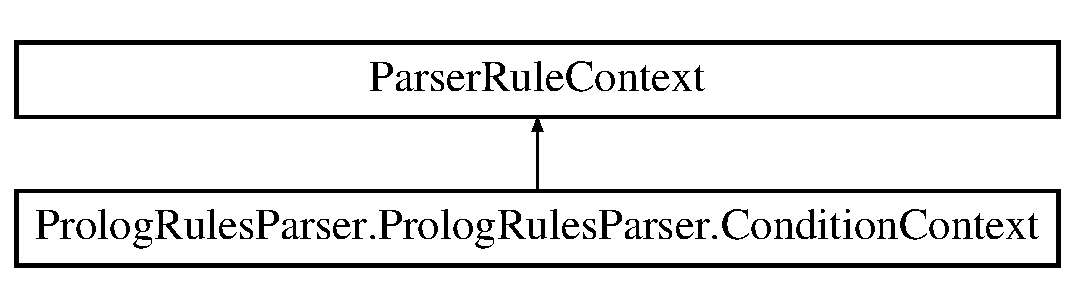
\includegraphics[height=2.000000cm]{class_prolog_rules_parser_1_1_prolog_rules_parser_1_1_condition_context}
\end{center}
\end{figure}
\subsection*{Public Member Functions}
\begin{DoxyCompactItemize}
\item 
def \hyperlink{class_prolog_rules_parser_1_1_prolog_rules_parser_1_1_condition_context_ae03e5d75176f30f9a8e3f70c287386b4}{\+\_\+\+\_\+init\+\_\+\+\_\+}
\item 
def \hyperlink{class_prolog_rules_parser_1_1_prolog_rules_parser_1_1_condition_context_a5c06a75d7e73d08a5dadc35409640503}{predicate} (self)
\item 
def \hyperlink{class_prolog_rules_parser_1_1_prolog_rules_parser_1_1_condition_context_addc4c9c67e6931c4a9cf80e71f593933}{predcount} (self)
\item 
def \hyperlink{class_prolog_rules_parser_1_1_prolog_rules_parser_1_1_condition_context_a0408cfbed4ca8052d500dd20999326f0}{comparator} (self)
\item 
def \hyperlink{class_prolog_rules_parser_1_1_prolog_rules_parser_1_1_condition_context_ad0965075e098339bbca3019598019ead}{negpred} (self)
\item 
def \hyperlink{class_prolog_rules_parser_1_1_prolog_rules_parser_1_1_condition_context_a27db3870e65df7e9c0ccf95d37e81e1d}{get\+Rule\+Index} (self)
\item 
def \hyperlink{class_prolog_rules_parser_1_1_prolog_rules_parser_1_1_condition_context_a1ec4b3cdaf62f4789adca36f5cc255fd}{enter\+Rule} (self, listener)
\item 
def \hyperlink{class_prolog_rules_parser_1_1_prolog_rules_parser_1_1_condition_context_a984b3b6a99946b419c8755271f200b4d}{exit\+Rule} (self, listener)
\end{DoxyCompactItemize}
\subsection*{Public Attributes}
\begin{DoxyCompactItemize}
\item 
\hyperlink{class_prolog_rules_parser_1_1_prolog_rules_parser_1_1_condition_context_a156a95efab49188bb3fc517537263c84}{parser}
\end{DoxyCompactItemize}


\subsection{Detailed Description}


Definition at line 735 of file Prolog\+Rules\+Parser.\+py.



\subsection{Constructor \& Destructor Documentation}
\hypertarget{class_prolog_rules_parser_1_1_prolog_rules_parser_1_1_condition_context_ae03e5d75176f30f9a8e3f70c287386b4}{}\index{Prolog\+Rules\+Parser\+::\+Prolog\+Rules\+Parser\+::\+Condition\+Context@{Prolog\+Rules\+Parser\+::\+Prolog\+Rules\+Parser\+::\+Condition\+Context}!\+\_\+\+\_\+init\+\_\+\+\_\+@{\+\_\+\+\_\+init\+\_\+\+\_\+}}
\index{\+\_\+\+\_\+init\+\_\+\+\_\+@{\+\_\+\+\_\+init\+\_\+\+\_\+}!Prolog\+Rules\+Parser\+::\+Prolog\+Rules\+Parser\+::\+Condition\+Context@{Prolog\+Rules\+Parser\+::\+Prolog\+Rules\+Parser\+::\+Condition\+Context}}
\subsubsection[{\+\_\+\+\_\+init\+\_\+\+\_\+}]{\setlength{\rightskip}{0pt plus 5cm}def Prolog\+Rules\+Parser.\+Prolog\+Rules\+Parser.\+Condition\+Context.\+\_\+\+\_\+init\+\_\+\+\_\+ (
\begin{DoxyParamCaption}
\item[{}]{self, }
\item[{}]{parser, }
\item[{}]{parent = {\ttfamily None}, }
\item[{}]{invoking\+State = {\ttfamily -\/1}}
\end{DoxyParamCaption}
)}\label{class_prolog_rules_parser_1_1_prolog_rules_parser_1_1_condition_context_ae03e5d75176f30f9a8e3f70c287386b4}


Definition at line 737 of file Prolog\+Rules\+Parser.\+py.



\subsection{Member Function Documentation}
\hypertarget{class_prolog_rules_parser_1_1_prolog_rules_parser_1_1_condition_context_a0408cfbed4ca8052d500dd20999326f0}{}\index{Prolog\+Rules\+Parser\+::\+Prolog\+Rules\+Parser\+::\+Condition\+Context@{Prolog\+Rules\+Parser\+::\+Prolog\+Rules\+Parser\+::\+Condition\+Context}!comparator@{comparator}}
\index{comparator@{comparator}!Prolog\+Rules\+Parser\+::\+Prolog\+Rules\+Parser\+::\+Condition\+Context@{Prolog\+Rules\+Parser\+::\+Prolog\+Rules\+Parser\+::\+Condition\+Context}}
\subsubsection[{comparator}]{\setlength{\rightskip}{0pt plus 5cm}def Prolog\+Rules\+Parser.\+Prolog\+Rules\+Parser.\+Condition\+Context.\+comparator (
\begin{DoxyParamCaption}
\item[{}]{self}
\end{DoxyParamCaption}
)}\label{class_prolog_rules_parser_1_1_prolog_rules_parser_1_1_condition_context_a0408cfbed4ca8052d500dd20999326f0}


Definition at line 749 of file Prolog\+Rules\+Parser.\+py.

\hypertarget{class_prolog_rules_parser_1_1_prolog_rules_parser_1_1_condition_context_a1ec4b3cdaf62f4789adca36f5cc255fd}{}\index{Prolog\+Rules\+Parser\+::\+Prolog\+Rules\+Parser\+::\+Condition\+Context@{Prolog\+Rules\+Parser\+::\+Prolog\+Rules\+Parser\+::\+Condition\+Context}!enter\+Rule@{enter\+Rule}}
\index{enter\+Rule@{enter\+Rule}!Prolog\+Rules\+Parser\+::\+Prolog\+Rules\+Parser\+::\+Condition\+Context@{Prolog\+Rules\+Parser\+::\+Prolog\+Rules\+Parser\+::\+Condition\+Context}}
\subsubsection[{enter\+Rule}]{\setlength{\rightskip}{0pt plus 5cm}def Prolog\+Rules\+Parser.\+Prolog\+Rules\+Parser.\+Condition\+Context.\+enter\+Rule (
\begin{DoxyParamCaption}
\item[{}]{self, }
\item[{}]{listener}
\end{DoxyParamCaption}
)}\label{class_prolog_rules_parser_1_1_prolog_rules_parser_1_1_condition_context_a1ec4b3cdaf62f4789adca36f5cc255fd}


Definition at line 760 of file Prolog\+Rules\+Parser.\+py.

\hypertarget{class_prolog_rules_parser_1_1_prolog_rules_parser_1_1_condition_context_a984b3b6a99946b419c8755271f200b4d}{}\index{Prolog\+Rules\+Parser\+::\+Prolog\+Rules\+Parser\+::\+Condition\+Context@{Prolog\+Rules\+Parser\+::\+Prolog\+Rules\+Parser\+::\+Condition\+Context}!exit\+Rule@{exit\+Rule}}
\index{exit\+Rule@{exit\+Rule}!Prolog\+Rules\+Parser\+::\+Prolog\+Rules\+Parser\+::\+Condition\+Context@{Prolog\+Rules\+Parser\+::\+Prolog\+Rules\+Parser\+::\+Condition\+Context}}
\subsubsection[{exit\+Rule}]{\setlength{\rightskip}{0pt plus 5cm}def Prolog\+Rules\+Parser.\+Prolog\+Rules\+Parser.\+Condition\+Context.\+exit\+Rule (
\begin{DoxyParamCaption}
\item[{}]{self, }
\item[{}]{listener}
\end{DoxyParamCaption}
)}\label{class_prolog_rules_parser_1_1_prolog_rules_parser_1_1_condition_context_a984b3b6a99946b419c8755271f200b4d}


Definition at line 764 of file Prolog\+Rules\+Parser.\+py.

\hypertarget{class_prolog_rules_parser_1_1_prolog_rules_parser_1_1_condition_context_a27db3870e65df7e9c0ccf95d37e81e1d}{}\index{Prolog\+Rules\+Parser\+::\+Prolog\+Rules\+Parser\+::\+Condition\+Context@{Prolog\+Rules\+Parser\+::\+Prolog\+Rules\+Parser\+::\+Condition\+Context}!get\+Rule\+Index@{get\+Rule\+Index}}
\index{get\+Rule\+Index@{get\+Rule\+Index}!Prolog\+Rules\+Parser\+::\+Prolog\+Rules\+Parser\+::\+Condition\+Context@{Prolog\+Rules\+Parser\+::\+Prolog\+Rules\+Parser\+::\+Condition\+Context}}
\subsubsection[{get\+Rule\+Index}]{\setlength{\rightskip}{0pt plus 5cm}def Prolog\+Rules\+Parser.\+Prolog\+Rules\+Parser.\+Condition\+Context.\+get\+Rule\+Index (
\begin{DoxyParamCaption}
\item[{}]{self}
\end{DoxyParamCaption}
)}\label{class_prolog_rules_parser_1_1_prolog_rules_parser_1_1_condition_context_a27db3870e65df7e9c0ccf95d37e81e1d}


Definition at line 757 of file Prolog\+Rules\+Parser.\+py.

\hypertarget{class_prolog_rules_parser_1_1_prolog_rules_parser_1_1_condition_context_ad0965075e098339bbca3019598019ead}{}\index{Prolog\+Rules\+Parser\+::\+Prolog\+Rules\+Parser\+::\+Condition\+Context@{Prolog\+Rules\+Parser\+::\+Prolog\+Rules\+Parser\+::\+Condition\+Context}!negpred@{negpred}}
\index{negpred@{negpred}!Prolog\+Rules\+Parser\+::\+Prolog\+Rules\+Parser\+::\+Condition\+Context@{Prolog\+Rules\+Parser\+::\+Prolog\+Rules\+Parser\+::\+Condition\+Context}}
\subsubsection[{negpred}]{\setlength{\rightskip}{0pt plus 5cm}def Prolog\+Rules\+Parser.\+Prolog\+Rules\+Parser.\+Condition\+Context.\+negpred (
\begin{DoxyParamCaption}
\item[{}]{self}
\end{DoxyParamCaption}
)}\label{class_prolog_rules_parser_1_1_prolog_rules_parser_1_1_condition_context_ad0965075e098339bbca3019598019ead}


Definition at line 753 of file Prolog\+Rules\+Parser.\+py.

\hypertarget{class_prolog_rules_parser_1_1_prolog_rules_parser_1_1_condition_context_addc4c9c67e6931c4a9cf80e71f593933}{}\index{Prolog\+Rules\+Parser\+::\+Prolog\+Rules\+Parser\+::\+Condition\+Context@{Prolog\+Rules\+Parser\+::\+Prolog\+Rules\+Parser\+::\+Condition\+Context}!predcount@{predcount}}
\index{predcount@{predcount}!Prolog\+Rules\+Parser\+::\+Prolog\+Rules\+Parser\+::\+Condition\+Context@{Prolog\+Rules\+Parser\+::\+Prolog\+Rules\+Parser\+::\+Condition\+Context}}
\subsubsection[{predcount}]{\setlength{\rightskip}{0pt plus 5cm}def Prolog\+Rules\+Parser.\+Prolog\+Rules\+Parser.\+Condition\+Context.\+predcount (
\begin{DoxyParamCaption}
\item[{}]{self}
\end{DoxyParamCaption}
)}\label{class_prolog_rules_parser_1_1_prolog_rules_parser_1_1_condition_context_addc4c9c67e6931c4a9cf80e71f593933}


Definition at line 745 of file Prolog\+Rules\+Parser.\+py.

\hypertarget{class_prolog_rules_parser_1_1_prolog_rules_parser_1_1_condition_context_a5c06a75d7e73d08a5dadc35409640503}{}\index{Prolog\+Rules\+Parser\+::\+Prolog\+Rules\+Parser\+::\+Condition\+Context@{Prolog\+Rules\+Parser\+::\+Prolog\+Rules\+Parser\+::\+Condition\+Context}!predicate@{predicate}}
\index{predicate@{predicate}!Prolog\+Rules\+Parser\+::\+Prolog\+Rules\+Parser\+::\+Condition\+Context@{Prolog\+Rules\+Parser\+::\+Prolog\+Rules\+Parser\+::\+Condition\+Context}}
\subsubsection[{predicate}]{\setlength{\rightskip}{0pt plus 5cm}def Prolog\+Rules\+Parser.\+Prolog\+Rules\+Parser.\+Condition\+Context.\+predicate (
\begin{DoxyParamCaption}
\item[{}]{self}
\end{DoxyParamCaption}
)}\label{class_prolog_rules_parser_1_1_prolog_rules_parser_1_1_condition_context_a5c06a75d7e73d08a5dadc35409640503}


Definition at line 741 of file Prolog\+Rules\+Parser.\+py.



\subsection{Member Data Documentation}
\hypertarget{class_prolog_rules_parser_1_1_prolog_rules_parser_1_1_condition_context_a156a95efab49188bb3fc517537263c84}{}\index{Prolog\+Rules\+Parser\+::\+Prolog\+Rules\+Parser\+::\+Condition\+Context@{Prolog\+Rules\+Parser\+::\+Prolog\+Rules\+Parser\+::\+Condition\+Context}!parser@{parser}}
\index{parser@{parser}!Prolog\+Rules\+Parser\+::\+Prolog\+Rules\+Parser\+::\+Condition\+Context@{Prolog\+Rules\+Parser\+::\+Prolog\+Rules\+Parser\+::\+Condition\+Context}}
\subsubsection[{parser}]{\setlength{\rightskip}{0pt plus 5cm}Prolog\+Rules\+Parser.\+Prolog\+Rules\+Parser.\+Condition\+Context.\+parser}\label{class_prolog_rules_parser_1_1_prolog_rules_parser_1_1_condition_context_a156a95efab49188bb3fc517537263c84}


Definition at line 739 of file Prolog\+Rules\+Parser.\+py.



The documentation for this class was generated from the following file\+:\begin{DoxyCompactItemize}
\item 
\hyperlink{_prolog_rules_parser_8py}{Prolog\+Rules\+Parser.\+py}\end{DoxyCompactItemize}

\hypertarget{class_prolog_rules_parser_1_1_prolog_rules_parser_1_1_constraint_context}{}\section{Prolog\+Rules\+Parser.\+Prolog\+Rules\+Parser.\+Constraint\+Context Class Reference}
\label{class_prolog_rules_parser_1_1_prolog_rules_parser_1_1_constraint_context}\index{Prolog\+Rules\+Parser.\+Prolog\+Rules\+Parser.\+Constraint\+Context@{Prolog\+Rules\+Parser.\+Prolog\+Rules\+Parser.\+Constraint\+Context}}
Inheritance diagram for Prolog\+Rules\+Parser.\+Prolog\+Rules\+Parser.\+Constraint\+Context\+:\begin{figure}[H]
\begin{center}
\leavevmode
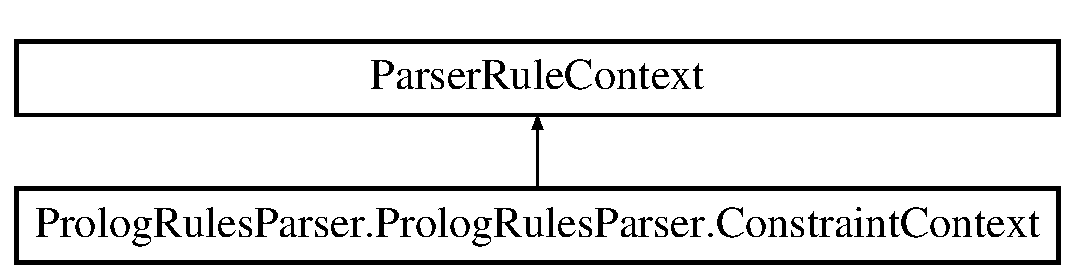
\includegraphics[height=2.000000cm]{class_prolog_rules_parser_1_1_prolog_rules_parser_1_1_constraint_context}
\end{center}
\end{figure}
\subsection*{Public Member Functions}
\begin{DoxyCompactItemize}
\item 
def \hyperlink{class_prolog_rules_parser_1_1_prolog_rules_parser_1_1_constraint_context_affde47cb52a237662e25e3470cf45d05}{\+\_\+\+\_\+init\+\_\+\+\_\+}
\item 
def \hyperlink{class_prolog_rules_parser_1_1_prolog_rules_parser_1_1_constraint_context_a765de48ee1268501a49732c770807e6f}{rulebody} (self)
\item 
def \hyperlink{class_prolog_rules_parser_1_1_prolog_rules_parser_1_1_constraint_context_a92d749fba377a4d930d7c407898314cd}{get\+Rule\+Index} (self)
\item 
def \hyperlink{class_prolog_rules_parser_1_1_prolog_rules_parser_1_1_constraint_context_a89a18bf2bd7a798c7b48e95fb1cd1785}{enter\+Rule} (self, listener)
\item 
def \hyperlink{class_prolog_rules_parser_1_1_prolog_rules_parser_1_1_constraint_context_a86e20df4333c8c8f72f03ddf80be4759}{exit\+Rule} (self, listener)
\end{DoxyCompactItemize}
\subsection*{Public Attributes}
\begin{DoxyCompactItemize}
\item 
\hyperlink{class_prolog_rules_parser_1_1_prolog_rules_parser_1_1_constraint_context_ac610adf034c82d60388f8bf8695c3f34}{parser}
\end{DoxyCompactItemize}


\subsection{Detailed Description}


Definition at line 297 of file Prolog\+Rules\+Parser.\+py.



\subsection{Constructor \& Destructor Documentation}
\hypertarget{class_prolog_rules_parser_1_1_prolog_rules_parser_1_1_constraint_context_affde47cb52a237662e25e3470cf45d05}{}\index{Prolog\+Rules\+Parser\+::\+Prolog\+Rules\+Parser\+::\+Constraint\+Context@{Prolog\+Rules\+Parser\+::\+Prolog\+Rules\+Parser\+::\+Constraint\+Context}!\+\_\+\+\_\+init\+\_\+\+\_\+@{\+\_\+\+\_\+init\+\_\+\+\_\+}}
\index{\+\_\+\+\_\+init\+\_\+\+\_\+@{\+\_\+\+\_\+init\+\_\+\+\_\+}!Prolog\+Rules\+Parser\+::\+Prolog\+Rules\+Parser\+::\+Constraint\+Context@{Prolog\+Rules\+Parser\+::\+Prolog\+Rules\+Parser\+::\+Constraint\+Context}}
\subsubsection[{\+\_\+\+\_\+init\+\_\+\+\_\+}]{\setlength{\rightskip}{0pt plus 5cm}def Prolog\+Rules\+Parser.\+Prolog\+Rules\+Parser.\+Constraint\+Context.\+\_\+\+\_\+init\+\_\+\+\_\+ (
\begin{DoxyParamCaption}
\item[{}]{self, }
\item[{}]{parser, }
\item[{}]{parent = {\ttfamily None}, }
\item[{}]{invoking\+State = {\ttfamily -\/1}}
\end{DoxyParamCaption}
)}\label{class_prolog_rules_parser_1_1_prolog_rules_parser_1_1_constraint_context_affde47cb52a237662e25e3470cf45d05}


Definition at line 299 of file Prolog\+Rules\+Parser.\+py.



\subsection{Member Function Documentation}
\hypertarget{class_prolog_rules_parser_1_1_prolog_rules_parser_1_1_constraint_context_a89a18bf2bd7a798c7b48e95fb1cd1785}{}\index{Prolog\+Rules\+Parser\+::\+Prolog\+Rules\+Parser\+::\+Constraint\+Context@{Prolog\+Rules\+Parser\+::\+Prolog\+Rules\+Parser\+::\+Constraint\+Context}!enter\+Rule@{enter\+Rule}}
\index{enter\+Rule@{enter\+Rule}!Prolog\+Rules\+Parser\+::\+Prolog\+Rules\+Parser\+::\+Constraint\+Context@{Prolog\+Rules\+Parser\+::\+Prolog\+Rules\+Parser\+::\+Constraint\+Context}}
\subsubsection[{enter\+Rule}]{\setlength{\rightskip}{0pt plus 5cm}def Prolog\+Rules\+Parser.\+Prolog\+Rules\+Parser.\+Constraint\+Context.\+enter\+Rule (
\begin{DoxyParamCaption}
\item[{}]{self, }
\item[{}]{listener}
\end{DoxyParamCaption}
)}\label{class_prolog_rules_parser_1_1_prolog_rules_parser_1_1_constraint_context_a89a18bf2bd7a798c7b48e95fb1cd1785}


Definition at line 310 of file Prolog\+Rules\+Parser.\+py.

\hypertarget{class_prolog_rules_parser_1_1_prolog_rules_parser_1_1_constraint_context_a86e20df4333c8c8f72f03ddf80be4759}{}\index{Prolog\+Rules\+Parser\+::\+Prolog\+Rules\+Parser\+::\+Constraint\+Context@{Prolog\+Rules\+Parser\+::\+Prolog\+Rules\+Parser\+::\+Constraint\+Context}!exit\+Rule@{exit\+Rule}}
\index{exit\+Rule@{exit\+Rule}!Prolog\+Rules\+Parser\+::\+Prolog\+Rules\+Parser\+::\+Constraint\+Context@{Prolog\+Rules\+Parser\+::\+Prolog\+Rules\+Parser\+::\+Constraint\+Context}}
\subsubsection[{exit\+Rule}]{\setlength{\rightskip}{0pt plus 5cm}def Prolog\+Rules\+Parser.\+Prolog\+Rules\+Parser.\+Constraint\+Context.\+exit\+Rule (
\begin{DoxyParamCaption}
\item[{}]{self, }
\item[{}]{listener}
\end{DoxyParamCaption}
)}\label{class_prolog_rules_parser_1_1_prolog_rules_parser_1_1_constraint_context_a86e20df4333c8c8f72f03ddf80be4759}


Definition at line 314 of file Prolog\+Rules\+Parser.\+py.

\hypertarget{class_prolog_rules_parser_1_1_prolog_rules_parser_1_1_constraint_context_a92d749fba377a4d930d7c407898314cd}{}\index{Prolog\+Rules\+Parser\+::\+Prolog\+Rules\+Parser\+::\+Constraint\+Context@{Prolog\+Rules\+Parser\+::\+Prolog\+Rules\+Parser\+::\+Constraint\+Context}!get\+Rule\+Index@{get\+Rule\+Index}}
\index{get\+Rule\+Index@{get\+Rule\+Index}!Prolog\+Rules\+Parser\+::\+Prolog\+Rules\+Parser\+::\+Constraint\+Context@{Prolog\+Rules\+Parser\+::\+Prolog\+Rules\+Parser\+::\+Constraint\+Context}}
\subsubsection[{get\+Rule\+Index}]{\setlength{\rightskip}{0pt plus 5cm}def Prolog\+Rules\+Parser.\+Prolog\+Rules\+Parser.\+Constraint\+Context.\+get\+Rule\+Index (
\begin{DoxyParamCaption}
\item[{}]{self}
\end{DoxyParamCaption}
)}\label{class_prolog_rules_parser_1_1_prolog_rules_parser_1_1_constraint_context_a92d749fba377a4d930d7c407898314cd}


Definition at line 307 of file Prolog\+Rules\+Parser.\+py.

\hypertarget{class_prolog_rules_parser_1_1_prolog_rules_parser_1_1_constraint_context_a765de48ee1268501a49732c770807e6f}{}\index{Prolog\+Rules\+Parser\+::\+Prolog\+Rules\+Parser\+::\+Constraint\+Context@{Prolog\+Rules\+Parser\+::\+Prolog\+Rules\+Parser\+::\+Constraint\+Context}!rulebody@{rulebody}}
\index{rulebody@{rulebody}!Prolog\+Rules\+Parser\+::\+Prolog\+Rules\+Parser\+::\+Constraint\+Context@{Prolog\+Rules\+Parser\+::\+Prolog\+Rules\+Parser\+::\+Constraint\+Context}}
\subsubsection[{rulebody}]{\setlength{\rightskip}{0pt plus 5cm}def Prolog\+Rules\+Parser.\+Prolog\+Rules\+Parser.\+Constraint\+Context.\+rulebody (
\begin{DoxyParamCaption}
\item[{}]{self}
\end{DoxyParamCaption}
)}\label{class_prolog_rules_parser_1_1_prolog_rules_parser_1_1_constraint_context_a765de48ee1268501a49732c770807e6f}


Definition at line 303 of file Prolog\+Rules\+Parser.\+py.



\subsection{Member Data Documentation}
\hypertarget{class_prolog_rules_parser_1_1_prolog_rules_parser_1_1_constraint_context_ac610adf034c82d60388f8bf8695c3f34}{}\index{Prolog\+Rules\+Parser\+::\+Prolog\+Rules\+Parser\+::\+Constraint\+Context@{Prolog\+Rules\+Parser\+::\+Prolog\+Rules\+Parser\+::\+Constraint\+Context}!parser@{parser}}
\index{parser@{parser}!Prolog\+Rules\+Parser\+::\+Prolog\+Rules\+Parser\+::\+Constraint\+Context@{Prolog\+Rules\+Parser\+::\+Prolog\+Rules\+Parser\+::\+Constraint\+Context}}
\subsubsection[{parser}]{\setlength{\rightskip}{0pt plus 5cm}Prolog\+Rules\+Parser.\+Prolog\+Rules\+Parser.\+Constraint\+Context.\+parser}\label{class_prolog_rules_parser_1_1_prolog_rules_parser_1_1_constraint_context_ac610adf034c82d60388f8bf8695c3f34}


Definition at line 301 of file Prolog\+Rules\+Parser.\+py.



The documentation for this class was generated from the following file\+:\begin{DoxyCompactItemize}
\item 
\hyperlink{_prolog_rules_parser_8py}{Prolog\+Rules\+Parser.\+py}\end{DoxyCompactItemize}

\hypertarget{classdemo__runner_1_1_demo_runner}{}\section{demo\+\_\+runner.\+Demo\+Runner Class Reference}
\label{classdemo__runner_1_1_demo_runner}\index{demo\+\_\+runner.\+Demo\+Runner@{demo\+\_\+runner.\+Demo\+Runner}}
Inheritance diagram for demo\+\_\+runner.\+Demo\+Runner\+:\begin{figure}[H]
\begin{center}
\leavevmode
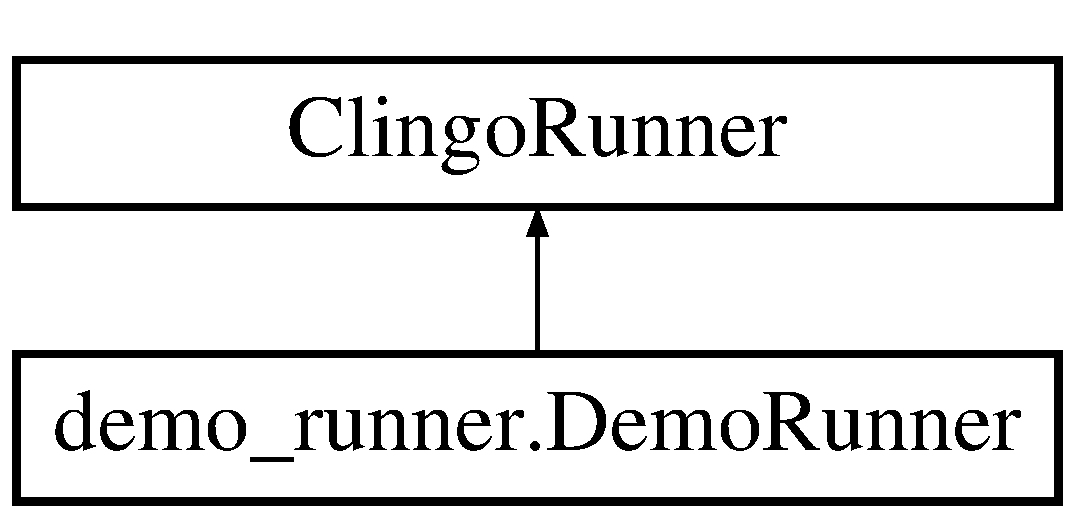
\includegraphics[height=2.000000cm]{classdemo__runner_1_1_demo_runner}
\end{center}
\end{figure}
\subsection*{Public Member Functions}
\begin{DoxyCompactItemize}
\item 
def \hyperlink{classdemo__runner_1_1_demo_runner_a21c31f98bb46783faa2636722961a344}{\+\_\+\+\_\+init\+\_\+\+\_\+} (self)
\item 
def \hyperlink{classdemo__runner_1_1_demo_runner_a641d478a6b05a3ec3bc459a76bbc7b0f}{get\+Heuristic\+Sequence} (self, param\+\_\+dict)
\item 
def \hyperlink{classdemo__runner_1_1_demo_runner_aae5ac02e28d9930588823a8db7bfb686}{get\+Required\+Features} (self, param\+\_\+dict)
\item 
def \hyperlink{classdemo__runner_1_1_demo_runner_a87805525af36312ea4e778a618dfe0d3}{write\+Solver\+Config\+File}
\item 
def \hyperlink{classdemo__runner_1_1_demo_runner_a6b2f4e4c2bd2320e18b103ea631fe361}{get\+Clingo\+Flags} (self, param\+\_\+dict)
\item 
def \hyperlink{classdemo__runner_1_1_demo_runner_aa0ed83d1e5ff19c2168fc4dbf5236266}{run\+Solver} (self)
\end{DoxyCompactItemize}
\subsection*{Public Attributes}
\begin{DoxyCompactItemize}
\item 
\hyperlink{classdemo__runner_1_1_demo_runner_af8316834678869878cfe909526261c32}{cmd\+\_\+line\+\_\+args}
\end{DoxyCompactItemize}
\subsection*{Static Public Attributes}
\begin{DoxyCompactItemize}
\item 
string \hyperlink{classdemo__runner_1_1_demo_runner_acd6a6464762d9c2fa38a02260b0d8c3e}{B\+A\+S\+E\+\_\+\+C\+O\+M\+M\+A\+N\+D} = \char`\"{}clingo eqn\+\_\+generator.\+lp -\/-\/outf=2 \char`\"{}
\item 
dictionary \hyperlink{classdemo__runner_1_1_demo_runner_a823a4fe7ebb0bbb8a25b7ae6966cf67f}{additional\+\_\+params} = \{ \textquotesingle{}heur\+Seq\textquotesingle{} \+: \textquotesingle{}\textquotesingle{}, \textquotesingle{}num\+Sets\textquotesingle{}\+: \textquotesingle{}1\textquotesingle{} , \textquotesingle{}clingo\textquotesingle{} \+: \textquotesingle{}\textquotesingle{}, \textquotesingle{}random\textquotesingle{} \+: \textquotesingle{}false\textquotesingle{}, \textquotesingle{}features\+File\textquotesingle{} \+: \textquotesingle{}None\textquotesingle{}, \textquotesingle{}json\+\_\+output\textquotesingle{}\+: \textquotesingle{}true\textquotesingle{}\}
\end{DoxyCompactItemize}


\subsection{Detailed Description}
\begin{DoxyVerb}Run clingo based on command line arguments\end{DoxyVerb}
 

Definition at line 3 of file demo\+\_\+runner.\+py.



\subsection{Constructor \& Destructor Documentation}
\hypertarget{classdemo__runner_1_1_demo_runner_a21c31f98bb46783faa2636722961a344}{}\index{demo\+\_\+runner\+::\+Demo\+Runner@{demo\+\_\+runner\+::\+Demo\+Runner}!\+\_\+\+\_\+init\+\_\+\+\_\+@{\+\_\+\+\_\+init\+\_\+\+\_\+}}
\index{\+\_\+\+\_\+init\+\_\+\+\_\+@{\+\_\+\+\_\+init\+\_\+\+\_\+}!demo\+\_\+runner\+::\+Demo\+Runner@{demo\+\_\+runner\+::\+Demo\+Runner}}
\subsubsection[{\+\_\+\+\_\+init\+\_\+\+\_\+}]{\setlength{\rightskip}{0pt plus 5cm}def demo\+\_\+runner.\+Demo\+Runner.\+\_\+\+\_\+init\+\_\+\+\_\+ (
\begin{DoxyParamCaption}
\item[{}]{self}
\end{DoxyParamCaption}
)}\label{classdemo__runner_1_1_demo_runner_a21c31f98bb46783faa2636722961a344}


Definition at line 7 of file demo\+\_\+runner.\+py.



\subsection{Member Function Documentation}
\hypertarget{classdemo__runner_1_1_demo_runner_a6b2f4e4c2bd2320e18b103ea631fe361}{}\index{demo\+\_\+runner\+::\+Demo\+Runner@{demo\+\_\+runner\+::\+Demo\+Runner}!get\+Clingo\+Flags@{get\+Clingo\+Flags}}
\index{get\+Clingo\+Flags@{get\+Clingo\+Flags}!demo\+\_\+runner\+::\+Demo\+Runner@{demo\+\_\+runner\+::\+Demo\+Runner}}
\subsubsection[{get\+Clingo\+Flags}]{\setlength{\rightskip}{0pt plus 5cm}def demo\+\_\+runner.\+Demo\+Runner.\+get\+Clingo\+Flags (
\begin{DoxyParamCaption}
\item[{}]{self, }
\item[{}]{param\+\_\+dict}
\end{DoxyParamCaption}
)}\label{classdemo__runner_1_1_demo_runner_a6b2f4e4c2bd2320e18b103ea631fe361}


Definition at line 35 of file demo\+\_\+runner.\+py.

\hypertarget{classdemo__runner_1_1_demo_runner_a641d478a6b05a3ec3bc459a76bbc7b0f}{}\index{demo\+\_\+runner\+::\+Demo\+Runner@{demo\+\_\+runner\+::\+Demo\+Runner}!get\+Heuristic\+Sequence@{get\+Heuristic\+Sequence}}
\index{get\+Heuristic\+Sequence@{get\+Heuristic\+Sequence}!demo\+\_\+runner\+::\+Demo\+Runner@{demo\+\_\+runner\+::\+Demo\+Runner}}
\subsubsection[{get\+Heuristic\+Sequence}]{\setlength{\rightskip}{0pt plus 5cm}def demo\+\_\+runner.\+Demo\+Runner.\+get\+Heuristic\+Sequence (
\begin{DoxyParamCaption}
\item[{}]{self, }
\item[{}]{param\+\_\+dict}
\end{DoxyParamCaption}
)}\label{classdemo__runner_1_1_demo_runner_a641d478a6b05a3ec3bc459a76bbc7b0f}


Definition at line 11 of file demo\+\_\+runner.\+py.

\hypertarget{classdemo__runner_1_1_demo_runner_aae5ac02e28d9930588823a8db7bfb686}{}\index{demo\+\_\+runner\+::\+Demo\+Runner@{demo\+\_\+runner\+::\+Demo\+Runner}!get\+Required\+Features@{get\+Required\+Features}}
\index{get\+Required\+Features@{get\+Required\+Features}!demo\+\_\+runner\+::\+Demo\+Runner@{demo\+\_\+runner\+::\+Demo\+Runner}}
\subsubsection[{get\+Required\+Features}]{\setlength{\rightskip}{0pt plus 5cm}def demo\+\_\+runner.\+Demo\+Runner.\+get\+Required\+Features (
\begin{DoxyParamCaption}
\item[{}]{self, }
\item[{}]{param\+\_\+dict}
\end{DoxyParamCaption}
)}\label{classdemo__runner_1_1_demo_runner_aae5ac02e28d9930588823a8db7bfb686}


Definition at line 21 of file demo\+\_\+runner.\+py.

\hypertarget{classdemo__runner_1_1_demo_runner_aa0ed83d1e5ff19c2168fc4dbf5236266}{}\index{demo\+\_\+runner\+::\+Demo\+Runner@{demo\+\_\+runner\+::\+Demo\+Runner}!run\+Solver@{run\+Solver}}
\index{run\+Solver@{run\+Solver}!demo\+\_\+runner\+::\+Demo\+Runner@{demo\+\_\+runner\+::\+Demo\+Runner}}
\subsubsection[{run\+Solver}]{\setlength{\rightskip}{0pt plus 5cm}def demo\+\_\+runner.\+Demo\+Runner.\+run\+Solver (
\begin{DoxyParamCaption}
\item[{}]{self}
\end{DoxyParamCaption}
)}\label{classdemo__runner_1_1_demo_runner_aa0ed83d1e5ff19c2168fc4dbf5236266}


Definition at line 45 of file demo\+\_\+runner.\+py.

\hypertarget{classdemo__runner_1_1_demo_runner_a87805525af36312ea4e778a618dfe0d3}{}\index{demo\+\_\+runner\+::\+Demo\+Runner@{demo\+\_\+runner\+::\+Demo\+Runner}!write\+Solver\+Config\+File@{write\+Solver\+Config\+File}}
\index{write\+Solver\+Config\+File@{write\+Solver\+Config\+File}!demo\+\_\+runner\+::\+Demo\+Runner@{demo\+\_\+runner\+::\+Demo\+Runner}}
\subsubsection[{write\+Solver\+Config\+File}]{\setlength{\rightskip}{0pt plus 5cm}def demo\+\_\+runner.\+Demo\+Runner.\+write\+Solver\+Config\+File (
\begin{DoxyParamCaption}
\item[{}]{self, }
\item[{}]{param\+\_\+dict, }
\item[{}]{filename = {\ttfamily \textquotesingle{}config\+\_\+params.lp\textquotesingle{}}}
\end{DoxyParamCaption}
)}\label{classdemo__runner_1_1_demo_runner_a87805525af36312ea4e778a618dfe0d3}


Definition at line 31 of file demo\+\_\+runner.\+py.



\subsection{Member Data Documentation}
\hypertarget{classdemo__runner_1_1_demo_runner_a823a4fe7ebb0bbb8a25b7ae6966cf67f}{}\index{demo\+\_\+runner\+::\+Demo\+Runner@{demo\+\_\+runner\+::\+Demo\+Runner}!additional\+\_\+params@{additional\+\_\+params}}
\index{additional\+\_\+params@{additional\+\_\+params}!demo\+\_\+runner\+::\+Demo\+Runner@{demo\+\_\+runner\+::\+Demo\+Runner}}
\subsubsection[{additional\+\_\+params}]{\setlength{\rightskip}{0pt plus 5cm}dictionary demo\+\_\+runner.\+Demo\+Runner.\+additional\+\_\+params = \{ \textquotesingle{}heur\+Seq\textquotesingle{} \+: \textquotesingle{}\textquotesingle{}, \textquotesingle{}num\+Sets\textquotesingle{}\+: \textquotesingle{}1\textquotesingle{} , \textquotesingle{}clingo\textquotesingle{} \+: \textquotesingle{}\textquotesingle{}, \textquotesingle{}random\textquotesingle{} \+: \textquotesingle{}false\textquotesingle{}, \textquotesingle{}features\+File\textquotesingle{} \+: \textquotesingle{}None\textquotesingle{}, \textquotesingle{}json\+\_\+output\textquotesingle{}\+: \textquotesingle{}true\textquotesingle{}\}\hspace{0.3cm}{\ttfamily [static]}}\label{classdemo__runner_1_1_demo_runner_a823a4fe7ebb0bbb8a25b7ae6966cf67f}


Definition at line 6 of file demo\+\_\+runner.\+py.

\hypertarget{classdemo__runner_1_1_demo_runner_acd6a6464762d9c2fa38a02260b0d8c3e}{}\index{demo\+\_\+runner\+::\+Demo\+Runner@{demo\+\_\+runner\+::\+Demo\+Runner}!B\+A\+S\+E\+\_\+\+C\+O\+M\+M\+A\+N\+D@{B\+A\+S\+E\+\_\+\+C\+O\+M\+M\+A\+N\+D}}
\index{B\+A\+S\+E\+\_\+\+C\+O\+M\+M\+A\+N\+D@{B\+A\+S\+E\+\_\+\+C\+O\+M\+M\+A\+N\+D}!demo\+\_\+runner\+::\+Demo\+Runner@{demo\+\_\+runner\+::\+Demo\+Runner}}
\subsubsection[{B\+A\+S\+E\+\_\+\+C\+O\+M\+M\+A\+N\+D}]{\setlength{\rightskip}{0pt plus 5cm}string demo\+\_\+runner.\+Demo\+Runner.\+B\+A\+S\+E\+\_\+\+C\+O\+M\+M\+A\+N\+D = \char`\"{}clingo eqn\+\_\+generator.\+lp -\/-\/outf=2 \char`\"{}\hspace{0.3cm}{\ttfamily [static]}}\label{classdemo__runner_1_1_demo_runner_acd6a6464762d9c2fa38a02260b0d8c3e}


Definition at line 5 of file demo\+\_\+runner.\+py.

\hypertarget{classdemo__runner_1_1_demo_runner_af8316834678869878cfe909526261c32}{}\index{demo\+\_\+runner\+::\+Demo\+Runner@{demo\+\_\+runner\+::\+Demo\+Runner}!cmd\+\_\+line\+\_\+args@{cmd\+\_\+line\+\_\+args}}
\index{cmd\+\_\+line\+\_\+args@{cmd\+\_\+line\+\_\+args}!demo\+\_\+runner\+::\+Demo\+Runner@{demo\+\_\+runner\+::\+Demo\+Runner}}
\subsubsection[{cmd\+\_\+line\+\_\+args}]{\setlength{\rightskip}{0pt plus 5cm}demo\+\_\+runner.\+Demo\+Runner.\+cmd\+\_\+line\+\_\+args}\label{classdemo__runner_1_1_demo_runner_af8316834678869878cfe909526261c32}


Definition at line 8 of file demo\+\_\+runner.\+py.



The documentation for this class was generated from the following file\+:\begin{DoxyCompactItemize}
\item 
\hyperlink{demo__runner_8py}{demo\+\_\+runner.\+py}\end{DoxyCompactItemize}

\hypertarget{classtotally__new__visualizer_1_1_equation_step_parser}{}\section{totally\+\_\+new\+\_\+visualizer.\+Equation\+Step\+Parser Class Reference}
\label{classtotally__new__visualizer_1_1_equation_step_parser}\index{totally\+\_\+new\+\_\+visualizer.\+Equation\+Step\+Parser@{totally\+\_\+new\+\_\+visualizer.\+Equation\+Step\+Parser}}


Parses predicates related to one step of a solution trace contains the data members\+: var\+\_\+str -- what variable an equation should be expressed with node\+\_\+data -- dictionary containing all node info parsed strategy\+\_\+data -- parsed explanations for the different strategy classes.  


\subsection*{Public Member Functions}
\begin{DoxyCompactItemize}
\item 
def \hyperlink{classtotally__new__visualizer_1_1_equation_step_parser_a025ac2e5112841d4b340029c120412f2}{\+\_\+\+\_\+init\+\_\+\+\_\+}
\item 
def \hyperlink{classtotally__new__visualizer_1_1_equation_step_parser_a7fd1c20efb5a99c2198f0731c9c9aba1}{update\+Variable} (self, new\+\_\+var)
\item 
def \hyperlink{classtotally__new__visualizer_1_1_equation_step_parser_acdeafbce50645287ac85046e93191c5a}{to\+Generated\+Step} (self)
\begin{DoxyCompactList}\small\item\em \hyperlink{classtotally__new__visualizer_1_1_equation_step_parser}{Equation\+Step\+Parser} contains lots of data we don\textquotesingle{}t need after parsing this method returns a Generated\+Step instance that has only what we want to save. \end{DoxyCompactList}\item 
def \hyperlink{classtotally__new__visualizer_1_1_equation_step_parser_a8e28e68df8ed9c7a34890d4ae6a6e2b9}{add\+Holds\+Predicate} (self, holds\+\_\+pred)
\begin{DoxyCompactList}\small\item\em save field/value info for a node that is expressed as a holds/2 predicate \end{DoxyCompactList}\item 
def \hyperlink{classtotally__new__visualizer_1_1_equation_step_parser_a0ea8c9f9125d10c34db60080cb98087e}{add\+Strategy\+Predicate} (self, pred\+\_\+obj)
\begin{DoxyCompactList}\small\item\em Add a predicate of the type \textquotesingle{}strategy\+Explanation\textquotesingle{}. \end{DoxyCompactList}\item 
def \hyperlink{classtotally__new__visualizer_1_1_equation_step_parser_ae60e437d9daae3ce0a8dae2fd8e60260}{add\+Parsed\+Predicate} (self, pred\+\_\+obj)
\begin{DoxyCompactList}\small\item\em Top level method called externally to add any predicate related to this time step. \end{DoxyCompactList}\item 
def \hyperlink{classtotally__new__visualizer_1_1_equation_step_parser_a0a9f53c1c140fecd4e5d6bd6bda9ae7e}{make\+Almost\+Fire\+Explanations} (self, model\+\_\+mgr)
\begin{DoxyCompactList}\small\item\em For every strategy we don\textquotesingle{}t have an explanation for, see if we have any \textquotesingle{}almost fire\textquotesingle{} explanations. \end{DoxyCompactList}\item 
def \hyperlink{classtotally__new__visualizer_1_1_equation_step_parser_a51372d5ce7c1fec1c4a1a7f7f8bfe3de}{make\+Almost\+Fire\+Explanation\+For} (self, strategy, model\+\_\+mgr)
\begin{DoxyCompactList}\small\item\em For a given strategy check all heuristics in that strategy type to see if any of them almost fire. \end{DoxyCompactList}\item 
def \hyperlink{classtotally__new__visualizer_1_1_equation_step_parser_aef1f6ba0922d50500fcf66e026effede}{post\+Process\+Step\+Data} (self, model\+\_\+mgr)
\begin{DoxyCompactList}\small\item\em handles all post-\/processing after step parser has received all predicates for this step N\+O\+T\+E\+: must be called externally \end{DoxyCompactList}\item 
def \hyperlink{classtotally__new__visualizer_1_1_equation_step_parser_ad4a30f362747a194b4f3e36ca5ddc238}{get\+Eqn\+String}
\item 
def \hyperlink{classtotally__new__visualizer_1_1_equation_step_parser_a25048323c9f80cbb0ea140985dfc1333}{translate\+Strategy\+Data} (self)
\begin{DoxyCompactList}\small\item\em use translator from \hyperlink{namespacetranslate__tree__nodes}{translate\+\_\+tree\+\_\+nodes} module to convert the node id\textquotesingle{}s in node\+\_\+data to a binary tree representation N\+O\+T\+E\+: this is necessary b/c Nell uses a binary tree to represent an equation but the internal nodes in my expression trees can have any number of children \end{DoxyCompactList}\item 
def \hyperlink{classtotally__new__visualizer_1_1_equation_step_parser_a3c973167ae47c603bf5f6ed2e04eea10}{make\+Explanation} (self, model\+\_\+mgr)
\begin{DoxyCompactList}\small\item\em uses model manager to lookup an explanation template for the action taken in this step, to explain why we can perform the selected operation for this step \end{DoxyCompactList}\item 
def \hyperlink{classtotally__new__visualizer_1_1_equation_step_parser_aef7a56859ca1922b836ddd56370288bb}{translate\+Single\+Explanation} (self, explanation\+\_\+sentences, translations)
\begin{DoxyCompactList}\small\item\em translates a single explanation array to use binary nodes an explanation array is a list of elements that look like\+: \mbox{[}explanation\+\_\+string, \mbox{[}list\+\_\+of\+\_\+operands\mbox{]}\mbox{]} \end{DoxyCompactList}\item 
def \hyperlink{classtotally__new__visualizer_1_1_equation_step_parser_aee458203f9e3923538d93d619a09894c}{translate\+List\+Of\+Strings} (self, string\+\_\+list, translations)
\begin{DoxyCompactList}\small\item\em translate a list of strings so nodes match a binary tree representation \end{DoxyCompactList}\item 
def \hyperlink{classtotally__new__visualizer_1_1_equation_step_parser_a4d4b598b9a729895cdaadae73f407d83}{make\+Eqn\+String} (self, root\+\_\+node)
\begin{DoxyCompactList}\small\item\em generates the string representation of a subexpression \end{DoxyCompactList}\item 
def \hyperlink{classtotally__new__visualizer_1_1_equation_step_parser_a2eb2f89d46d274c80c7930a5f5fc9623}{make\+Monomial} (self, node\+\_\+name)
\end{DoxyCompactItemize}
\subsection*{Static Public Member Functions}
\begin{DoxyCompactItemize}
\item 
def \hyperlink{classtotally__new__visualizer_1_1_equation_step_parser_a8aaaf60180dffc7f531cd56df9bcc891}{make\+Monomial\+From\+Data}
\begin{DoxyCompactList}\small\item\em make a monomial string \end{DoxyCompactList}\end{DoxyCompactItemize}
\subsection*{Public Attributes}
\begin{DoxyCompactItemize}
\item 
\hyperlink{classtotally__new__visualizer_1_1_equation_step_parser_a021358bd55a4cea135012d4a83138711}{var\+\_\+str}
\item 
\hyperlink{classtotally__new__visualizer_1_1_equation_step_parser_ad7bb7147eedff025bb568ecb8826ce08}{node\+\_\+data}
\item 
\hyperlink{classtotally__new__visualizer_1_1_equation_step_parser_a9fd629de7e40b3f7764fb91e9d1c7962}{misc\+\_\+data}
\item 
\hyperlink{classtotally__new__visualizer_1_1_equation_step_parser_ac5cad9ea5ae6ed0d1c86a506b0a0e76e}{strategy\+\_\+data}
\item 
\hyperlink{classtotally__new__visualizer_1_1_equation_step_parser_a1d2445c87a6b9d8400ef8c78ea2e5919}{optimal\+\_\+action}
\item 
\hyperlink{classtotally__new__visualizer_1_1_equation_step_parser_adcf8eb027974aa76205cbd1e42604919}{optimal\+\_\+operands}
\end{DoxyCompactItemize}


\subsection{Detailed Description}
Parses predicates related to one step of a solution trace contains the data members\+: var\+\_\+str -- what variable an equation should be expressed with node\+\_\+data -- dictionary containing all node info parsed strategy\+\_\+data -- parsed explanations for the different strategy classes. 

Definition at line 43 of file totally\+\_\+new\+\_\+visualizer.\+py.



\subsection{Constructor \& Destructor Documentation}
\hypertarget{classtotally__new__visualizer_1_1_equation_step_parser_a025ac2e5112841d4b340029c120412f2}{}\index{totally\+\_\+new\+\_\+visualizer\+::\+Equation\+Step\+Parser@{totally\+\_\+new\+\_\+visualizer\+::\+Equation\+Step\+Parser}!\+\_\+\+\_\+init\+\_\+\+\_\+@{\+\_\+\+\_\+init\+\_\+\+\_\+}}
\index{\+\_\+\+\_\+init\+\_\+\+\_\+@{\+\_\+\+\_\+init\+\_\+\+\_\+}!totally\+\_\+new\+\_\+visualizer\+::\+Equation\+Step\+Parser@{totally\+\_\+new\+\_\+visualizer\+::\+Equation\+Step\+Parser}}
\subsubsection[{\+\_\+\+\_\+init\+\_\+\+\_\+}]{\setlength{\rightskip}{0pt plus 5cm}def totally\+\_\+new\+\_\+visualizer.\+Equation\+Step\+Parser.\+\_\+\+\_\+init\+\_\+\+\_\+ (
\begin{DoxyParamCaption}
\item[{}]{self, }
\item[{}]{var\+\_\+str = {\ttfamily \textquotesingle{}x\textquotesingle{}}}
\end{DoxyParamCaption}
)}\label{classtotally__new__visualizer_1_1_equation_step_parser_a025ac2e5112841d4b340029c120412f2}

\begin{DoxyParams}[1]{Parameters}
\mbox{\tt in}  & {\em var\+\_\+str} & variable to use when constructing equation (typically it\textquotesingle{}s \textquotesingle{}x\textquotesingle{} or \textquotesingle{}y\textquotesingle{}) \\
\hline
\end{DoxyParams}


Definition at line 46 of file totally\+\_\+new\+\_\+visualizer.\+py.



\subsection{Member Function Documentation}
\hypertarget{classtotally__new__visualizer_1_1_equation_step_parser_a8e28e68df8ed9c7a34890d4ae6a6e2b9}{}\index{totally\+\_\+new\+\_\+visualizer\+::\+Equation\+Step\+Parser@{totally\+\_\+new\+\_\+visualizer\+::\+Equation\+Step\+Parser}!add\+Holds\+Predicate@{add\+Holds\+Predicate}}
\index{add\+Holds\+Predicate@{add\+Holds\+Predicate}!totally\+\_\+new\+\_\+visualizer\+::\+Equation\+Step\+Parser@{totally\+\_\+new\+\_\+visualizer\+::\+Equation\+Step\+Parser}}
\subsubsection[{add\+Holds\+Predicate}]{\setlength{\rightskip}{0pt plus 5cm}def totally\+\_\+new\+\_\+visualizer.\+Equation\+Step\+Parser.\+add\+Holds\+Predicate (
\begin{DoxyParamCaption}
\item[{}]{self, }
\item[{}]{holds\+\_\+pred}
\end{DoxyParamCaption}
)}\label{classtotally__new__visualizer_1_1_equation_step_parser_a8e28e68df8ed9c7a34890d4ae6a6e2b9}


save field/value info for a node that is expressed as a holds/2 predicate 



Definition at line 72 of file totally\+\_\+new\+\_\+visualizer.\+py.

\hypertarget{classtotally__new__visualizer_1_1_equation_step_parser_ae60e437d9daae3ce0a8dae2fd8e60260}{}\index{totally\+\_\+new\+\_\+visualizer\+::\+Equation\+Step\+Parser@{totally\+\_\+new\+\_\+visualizer\+::\+Equation\+Step\+Parser}!add\+Parsed\+Predicate@{add\+Parsed\+Predicate}}
\index{add\+Parsed\+Predicate@{add\+Parsed\+Predicate}!totally\+\_\+new\+\_\+visualizer\+::\+Equation\+Step\+Parser@{totally\+\_\+new\+\_\+visualizer\+::\+Equation\+Step\+Parser}}
\subsubsection[{add\+Parsed\+Predicate}]{\setlength{\rightskip}{0pt plus 5cm}def totally\+\_\+new\+\_\+visualizer.\+Equation\+Step\+Parser.\+add\+Parsed\+Predicate (
\begin{DoxyParamCaption}
\item[{}]{self, }
\item[{}]{pred\+\_\+obj}
\end{DoxyParamCaption}
)}\label{classtotally__new__visualizer_1_1_equation_step_parser_ae60e437d9daae3ce0a8dae2fd8e60260}


Top level method called externally to add any predicate related to this time step. 


\begin{DoxyParams}[1]{Parameters}
\mbox{\tt in}  & {\em pred\+\_\+obj} & an instance of Predicate namedtuple in \hyperlink{namespacepred__parser}{pred\+\_\+parser} module \\
\hline
\end{DoxyParams}


Definition at line 110 of file totally\+\_\+new\+\_\+visualizer.\+py.

\hypertarget{classtotally__new__visualizer_1_1_equation_step_parser_a0ea8c9f9125d10c34db60080cb98087e}{}\index{totally\+\_\+new\+\_\+visualizer\+::\+Equation\+Step\+Parser@{totally\+\_\+new\+\_\+visualizer\+::\+Equation\+Step\+Parser}!add\+Strategy\+Predicate@{add\+Strategy\+Predicate}}
\index{add\+Strategy\+Predicate@{add\+Strategy\+Predicate}!totally\+\_\+new\+\_\+visualizer\+::\+Equation\+Step\+Parser@{totally\+\_\+new\+\_\+visualizer\+::\+Equation\+Step\+Parser}}
\subsubsection[{add\+Strategy\+Predicate}]{\setlength{\rightskip}{0pt plus 5cm}def totally\+\_\+new\+\_\+visualizer.\+Equation\+Step\+Parser.\+add\+Strategy\+Predicate (
\begin{DoxyParamCaption}
\item[{}]{self, }
\item[{}]{pred\+\_\+obj}
\end{DoxyParamCaption}
)}\label{classtotally__new__visualizer_1_1_equation_step_parser_a0ea8c9f9125d10c34db60080cb98087e}


Add a predicate of the type \textquotesingle{}strategy\+Explanation\textquotesingle{}. 

These predicates help explain why a certain operation was chosen over others 
\begin{DoxyParams}[1]{Parameters}
\mbox{\tt in}  & {\em pred\+\_\+obj} & an instance of Predicate namedtuple in \hyperlink{namespacepred__parser}{pred\+\_\+parser} module \\
\hline
\end{DoxyParams}


Definition at line 88 of file totally\+\_\+new\+\_\+visualizer.\+py.

\hypertarget{classtotally__new__visualizer_1_1_equation_step_parser_ad4a30f362747a194b4f3e36ca5ddc238}{}\index{totally\+\_\+new\+\_\+visualizer\+::\+Equation\+Step\+Parser@{totally\+\_\+new\+\_\+visualizer\+::\+Equation\+Step\+Parser}!get\+Eqn\+String@{get\+Eqn\+String}}
\index{get\+Eqn\+String@{get\+Eqn\+String}!totally\+\_\+new\+\_\+visualizer\+::\+Equation\+Step\+Parser@{totally\+\_\+new\+\_\+visualizer\+::\+Equation\+Step\+Parser}}
\subsubsection[{get\+Eqn\+String}]{\setlength{\rightskip}{0pt plus 5cm}def totally\+\_\+new\+\_\+visualizer.\+Equation\+Step\+Parser.\+get\+Eqn\+String (
\begin{DoxyParamCaption}
\item[{}]{self, }
\item[{}]{as\+\_\+latex = {\ttfamily False}, }
\item[{}]{json\+\_\+output = {\ttfamily False}}
\end{DoxyParamCaption}
)}\label{classtotally__new__visualizer_1_1_equation_step_parser_ad4a30f362747a194b4f3e36ca5ddc238}

\begin{DoxyParams}[1]{Parameters}
\mbox{\tt in}  & {\em as\+\_\+latex} & depricated \\
\hline
\mbox{\tt in}  & {\em json\+\_\+output} & depricated \\
\hline
\end{DoxyParams}
\begin{DoxyReturn}{Returns}
a string representation of the equation at this step 
\end{DoxyReturn}


Definition at line 182 of file totally\+\_\+new\+\_\+visualizer.\+py.

\hypertarget{classtotally__new__visualizer_1_1_equation_step_parser_a51372d5ce7c1fec1c4a1a7f7f8bfe3de}{}\index{totally\+\_\+new\+\_\+visualizer\+::\+Equation\+Step\+Parser@{totally\+\_\+new\+\_\+visualizer\+::\+Equation\+Step\+Parser}!make\+Almost\+Fire\+Explanation\+For@{make\+Almost\+Fire\+Explanation\+For}}
\index{make\+Almost\+Fire\+Explanation\+For@{make\+Almost\+Fire\+Explanation\+For}!totally\+\_\+new\+\_\+visualizer\+::\+Equation\+Step\+Parser@{totally\+\_\+new\+\_\+visualizer\+::\+Equation\+Step\+Parser}}
\subsubsection[{make\+Almost\+Fire\+Explanation\+For}]{\setlength{\rightskip}{0pt plus 5cm}def totally\+\_\+new\+\_\+visualizer.\+Equation\+Step\+Parser.\+make\+Almost\+Fire\+Explanation\+For (
\begin{DoxyParamCaption}
\item[{}]{self, }
\item[{}]{strategy, }
\item[{}]{model\+\_\+mgr}
\end{DoxyParamCaption}
)}\label{classtotally__new__visualizer_1_1_equation_step_parser_a51372d5ce7c1fec1c4a1a7f7f8bfe3de}


For a given strategy check all heuristics in that strategy type to see if any of them almost fire. 


\begin{DoxyParams}[1]{Parameters}
\mbox{\tt in}  & {\em strategy} & string representing strategy class \\
\hline
\mbox{\tt in}  & {\em model\+\_\+mgr} & manages all predicates true for this time step \\
\hline
\end{DoxyParams}


Definition at line 149 of file totally\+\_\+new\+\_\+visualizer.\+py.

\hypertarget{classtotally__new__visualizer_1_1_equation_step_parser_a0a9f53c1c140fecd4e5d6bd6bda9ae7e}{}\index{totally\+\_\+new\+\_\+visualizer\+::\+Equation\+Step\+Parser@{totally\+\_\+new\+\_\+visualizer\+::\+Equation\+Step\+Parser}!make\+Almost\+Fire\+Explanations@{make\+Almost\+Fire\+Explanations}}
\index{make\+Almost\+Fire\+Explanations@{make\+Almost\+Fire\+Explanations}!totally\+\_\+new\+\_\+visualizer\+::\+Equation\+Step\+Parser@{totally\+\_\+new\+\_\+visualizer\+::\+Equation\+Step\+Parser}}
\subsubsection[{make\+Almost\+Fire\+Explanations}]{\setlength{\rightskip}{0pt plus 5cm}def totally\+\_\+new\+\_\+visualizer.\+Equation\+Step\+Parser.\+make\+Almost\+Fire\+Explanations (
\begin{DoxyParamCaption}
\item[{}]{self, }
\item[{}]{model\+\_\+mgr}
\end{DoxyParamCaption}
)}\label{classtotally__new__visualizer_1_1_equation_step_parser_a0a9f53c1c140fecd4e5d6bd6bda9ae7e}


For every strategy we don\textquotesingle{}t have an explanation for, see if we have any \textquotesingle{}almost fire\textquotesingle{} explanations. 


\begin{DoxyParams}[1]{Parameters}
\mbox{\tt in}  & {\em model\+\_\+mgr} & manages all predicates true for this time step \\
\hline
\end{DoxyParams}


Definition at line 139 of file totally\+\_\+new\+\_\+visualizer.\+py.

\hypertarget{classtotally__new__visualizer_1_1_equation_step_parser_a4d4b598b9a729895cdaadae73f407d83}{}\index{totally\+\_\+new\+\_\+visualizer\+::\+Equation\+Step\+Parser@{totally\+\_\+new\+\_\+visualizer\+::\+Equation\+Step\+Parser}!make\+Eqn\+String@{make\+Eqn\+String}}
\index{make\+Eqn\+String@{make\+Eqn\+String}!totally\+\_\+new\+\_\+visualizer\+::\+Equation\+Step\+Parser@{totally\+\_\+new\+\_\+visualizer\+::\+Equation\+Step\+Parser}}
\subsubsection[{make\+Eqn\+String}]{\setlength{\rightskip}{0pt plus 5cm}def totally\+\_\+new\+\_\+visualizer.\+Equation\+Step\+Parser.\+make\+Eqn\+String (
\begin{DoxyParamCaption}
\item[{}]{self, }
\item[{}]{root\+\_\+node}
\end{DoxyParamCaption}
)}\label{classtotally__new__visualizer_1_1_equation_step_parser_a4d4b598b9a729895cdaadae73f407d83}


generates the string representation of a subexpression 


\begin{DoxyParams}[1]{Parameters}
\mbox{\tt in}  & {\em root\+\_\+node} & the node id (ex\+: \textquotesingle{}id(1,2)\textquotesingle{} ) of the subexpression\textquotesingle{}s root \\
\hline
\end{DoxyParams}
\begin{DoxyReturn}{Returns}
a string representing the subexpression 
\end{DoxyReturn}


Definition at line 269 of file totally\+\_\+new\+\_\+visualizer.\+py.

\hypertarget{classtotally__new__visualizer_1_1_equation_step_parser_a3c973167ae47c603bf5f6ed2e04eea10}{}\index{totally\+\_\+new\+\_\+visualizer\+::\+Equation\+Step\+Parser@{totally\+\_\+new\+\_\+visualizer\+::\+Equation\+Step\+Parser}!make\+Explanation@{make\+Explanation}}
\index{make\+Explanation@{make\+Explanation}!totally\+\_\+new\+\_\+visualizer\+::\+Equation\+Step\+Parser@{totally\+\_\+new\+\_\+visualizer\+::\+Equation\+Step\+Parser}}
\subsubsection[{make\+Explanation}]{\setlength{\rightskip}{0pt plus 5cm}def totally\+\_\+new\+\_\+visualizer.\+Equation\+Step\+Parser.\+make\+Explanation (
\begin{DoxyParamCaption}
\item[{}]{self, }
\item[{}]{model\+\_\+mgr}
\end{DoxyParamCaption}
)}\label{classtotally__new__visualizer_1_1_equation_step_parser_a3c973167ae47c603bf5f6ed2e04eea10}


uses model manager to lookup an explanation template for the action taken in this step, to explain why we can perform the selected operation for this step 



Definition at line 221 of file totally\+\_\+new\+\_\+visualizer.\+py.

\hypertarget{classtotally__new__visualizer_1_1_equation_step_parser_a2eb2f89d46d274c80c7930a5f5fc9623}{}\index{totally\+\_\+new\+\_\+visualizer\+::\+Equation\+Step\+Parser@{totally\+\_\+new\+\_\+visualizer\+::\+Equation\+Step\+Parser}!make\+Monomial@{make\+Monomial}}
\index{make\+Monomial@{make\+Monomial}!totally\+\_\+new\+\_\+visualizer\+::\+Equation\+Step\+Parser@{totally\+\_\+new\+\_\+visualizer\+::\+Equation\+Step\+Parser}}
\subsubsection[{make\+Monomial}]{\setlength{\rightskip}{0pt plus 5cm}def totally\+\_\+new\+\_\+visualizer.\+Equation\+Step\+Parser.\+make\+Monomial (
\begin{DoxyParamCaption}
\item[{}]{self, }
\item[{}]{node\+\_\+name}
\end{DoxyParamCaption}
)}\label{classtotally__new__visualizer_1_1_equation_step_parser_a2eb2f89d46d274c80c7930a5f5fc9623}

\begin{DoxyParams}[1]{Parameters}
\mbox{\tt in}  & {\em node\+\_\+name} & the node id to get a monomial string for \\
\hline
\end{DoxyParams}
\begin{DoxyReturn}{Returns}
the monomial string representing the given node id\begin{DoxyVerb}Given a node name, construct the monomial referenced by that node\end{DoxyVerb}
 
\end{DoxyReturn}


Definition at line 315 of file totally\+\_\+new\+\_\+visualizer.\+py.

\hypertarget{classtotally__new__visualizer_1_1_equation_step_parser_a8aaaf60180dffc7f531cd56df9bcc891}{}\index{totally\+\_\+new\+\_\+visualizer\+::\+Equation\+Step\+Parser@{totally\+\_\+new\+\_\+visualizer\+::\+Equation\+Step\+Parser}!make\+Monomial\+From\+Data@{make\+Monomial\+From\+Data}}
\index{make\+Monomial\+From\+Data@{make\+Monomial\+From\+Data}!totally\+\_\+new\+\_\+visualizer\+::\+Equation\+Step\+Parser@{totally\+\_\+new\+\_\+visualizer\+::\+Equation\+Step\+Parser}}
\subsubsection[{make\+Monomial\+From\+Data}]{\setlength{\rightskip}{0pt plus 5cm}def totally\+\_\+new\+\_\+visualizer.\+Equation\+Step\+Parser.\+make\+Monomial\+From\+Data (
\begin{DoxyParamCaption}
\item[{}]{deg, }
\item[{}]{coeff, }
\item[{}]{var\+\_\+str = {\ttfamily \textquotesingle{}x\textquotesingle{}}}
\end{DoxyParamCaption}
)\hspace{0.3cm}{\ttfamily [static]}}\label{classtotally__new__visualizer_1_1_equation_step_parser_a8aaaf60180dffc7f531cd56df9bcc891}


make a monomial string 


\begin{DoxyParams}[1]{Parameters}
\mbox{\tt in}  & {\em deg} & string representing degree \\
\hline
\mbox{\tt in}  & {\em coeff} & string representing coefficient \\
\hline
\mbox{\tt in}  & {\em var\+\_\+str} & string representing what variable name to use \\
\hline
\end{DoxyParams}


Definition at line 296 of file totally\+\_\+new\+\_\+visualizer.\+py.

\hypertarget{classtotally__new__visualizer_1_1_equation_step_parser_aef1f6ba0922d50500fcf66e026effede}{}\index{totally\+\_\+new\+\_\+visualizer\+::\+Equation\+Step\+Parser@{totally\+\_\+new\+\_\+visualizer\+::\+Equation\+Step\+Parser}!post\+Process\+Step\+Data@{post\+Process\+Step\+Data}}
\index{post\+Process\+Step\+Data@{post\+Process\+Step\+Data}!totally\+\_\+new\+\_\+visualizer\+::\+Equation\+Step\+Parser@{totally\+\_\+new\+\_\+visualizer\+::\+Equation\+Step\+Parser}}
\subsubsection[{post\+Process\+Step\+Data}]{\setlength{\rightskip}{0pt plus 5cm}def totally\+\_\+new\+\_\+visualizer.\+Equation\+Step\+Parser.\+post\+Process\+Step\+Data (
\begin{DoxyParamCaption}
\item[{}]{self, }
\item[{}]{model\+\_\+mgr}
\end{DoxyParamCaption}
)}\label{classtotally__new__visualizer_1_1_equation_step_parser_aef1f6ba0922d50500fcf66e026effede}


handles all post-\/processing after step parser has received all predicates for this step N\+O\+T\+E\+: must be called externally 



Definition at line 163 of file totally\+\_\+new\+\_\+visualizer.\+py.

\hypertarget{classtotally__new__visualizer_1_1_equation_step_parser_acdeafbce50645287ac85046e93191c5a}{}\index{totally\+\_\+new\+\_\+visualizer\+::\+Equation\+Step\+Parser@{totally\+\_\+new\+\_\+visualizer\+::\+Equation\+Step\+Parser}!to\+Generated\+Step@{to\+Generated\+Step}}
\index{to\+Generated\+Step@{to\+Generated\+Step}!totally\+\_\+new\+\_\+visualizer\+::\+Equation\+Step\+Parser@{totally\+\_\+new\+\_\+visualizer\+::\+Equation\+Step\+Parser}}
\subsubsection[{to\+Generated\+Step}]{\setlength{\rightskip}{0pt plus 5cm}def totally\+\_\+new\+\_\+visualizer.\+Equation\+Step\+Parser.\+to\+Generated\+Step (
\begin{DoxyParamCaption}
\item[{}]{self}
\end{DoxyParamCaption}
)}\label{classtotally__new__visualizer_1_1_equation_step_parser_acdeafbce50645287ac85046e93191c5a}


\hyperlink{classtotally__new__visualizer_1_1_equation_step_parser}{Equation\+Step\+Parser} contains lots of data we don\textquotesingle{}t need after parsing this method returns a Generated\+Step instance that has only what we want to save. 



Definition at line 65 of file totally\+\_\+new\+\_\+visualizer.\+py.

\hypertarget{classtotally__new__visualizer_1_1_equation_step_parser_aee458203f9e3923538d93d619a09894c}{}\index{totally\+\_\+new\+\_\+visualizer\+::\+Equation\+Step\+Parser@{totally\+\_\+new\+\_\+visualizer\+::\+Equation\+Step\+Parser}!translate\+List\+Of\+Strings@{translate\+List\+Of\+Strings}}
\index{translate\+List\+Of\+Strings@{translate\+List\+Of\+Strings}!totally\+\_\+new\+\_\+visualizer\+::\+Equation\+Step\+Parser@{totally\+\_\+new\+\_\+visualizer\+::\+Equation\+Step\+Parser}}
\subsubsection[{translate\+List\+Of\+Strings}]{\setlength{\rightskip}{0pt plus 5cm}def totally\+\_\+new\+\_\+visualizer.\+Equation\+Step\+Parser.\+translate\+List\+Of\+Strings (
\begin{DoxyParamCaption}
\item[{}]{self, }
\item[{}]{string\+\_\+list, }
\item[{}]{translations}
\end{DoxyParamCaption}
)}\label{classtotally__new__visualizer_1_1_equation_step_parser_aee458203f9e3923538d93d619a09894c}


translate a list of strings so nodes match a binary tree representation 



Definition at line 261 of file totally\+\_\+new\+\_\+visualizer.\+py.

\hypertarget{classtotally__new__visualizer_1_1_equation_step_parser_aef7a56859ca1922b836ddd56370288bb}{}\index{totally\+\_\+new\+\_\+visualizer\+::\+Equation\+Step\+Parser@{totally\+\_\+new\+\_\+visualizer\+::\+Equation\+Step\+Parser}!translate\+Single\+Explanation@{translate\+Single\+Explanation}}
\index{translate\+Single\+Explanation@{translate\+Single\+Explanation}!totally\+\_\+new\+\_\+visualizer\+::\+Equation\+Step\+Parser@{totally\+\_\+new\+\_\+visualizer\+::\+Equation\+Step\+Parser}}
\subsubsection[{translate\+Single\+Explanation}]{\setlength{\rightskip}{0pt plus 5cm}def totally\+\_\+new\+\_\+visualizer.\+Equation\+Step\+Parser.\+translate\+Single\+Explanation (
\begin{DoxyParamCaption}
\item[{}]{self, }
\item[{}]{explanation\+\_\+sentences, }
\item[{}]{translations}
\end{DoxyParamCaption}
)}\label{classtotally__new__visualizer_1_1_equation_step_parser_aef7a56859ca1922b836ddd56370288bb}


translates a single explanation array to use binary nodes an explanation array is a list of elements that look like\+: \mbox{[}explanation\+\_\+string, \mbox{[}list\+\_\+of\+\_\+operands\mbox{]}\mbox{]} 


\begin{DoxyParams}[1]{Parameters}
\mbox{\tt in}  & {\em explanation\+\_\+sentences} & a list of \mbox{[}explanation\+\_\+string, \mbox{[}list\+\_\+of\+\_\+operands\mbox{]}\mbox{]} elements \\
\hline
\mbox{\tt in}  & {\em translations} & a hashmap with mappings old\+\_\+node\+\_\+id --$>$ new\+\_\+node\+\_\+id \\
\hline
\end{DoxyParams}
\begin{DoxyReturn}{Returns}
a list of explanation sentences with the nodes changed to Nell\textquotesingle{}s format 
\end{DoxyReturn}


Definition at line 253 of file totally\+\_\+new\+\_\+visualizer.\+py.

\hypertarget{classtotally__new__visualizer_1_1_equation_step_parser_a25048323c9f80cbb0ea140985dfc1333}{}\index{totally\+\_\+new\+\_\+visualizer\+::\+Equation\+Step\+Parser@{totally\+\_\+new\+\_\+visualizer\+::\+Equation\+Step\+Parser}!translate\+Strategy\+Data@{translate\+Strategy\+Data}}
\index{translate\+Strategy\+Data@{translate\+Strategy\+Data}!totally\+\_\+new\+\_\+visualizer\+::\+Equation\+Step\+Parser@{totally\+\_\+new\+\_\+visualizer\+::\+Equation\+Step\+Parser}}
\subsubsection[{translate\+Strategy\+Data}]{\setlength{\rightskip}{0pt plus 5cm}def totally\+\_\+new\+\_\+visualizer.\+Equation\+Step\+Parser.\+translate\+Strategy\+Data (
\begin{DoxyParamCaption}
\item[{}]{self}
\end{DoxyParamCaption}
)}\label{classtotally__new__visualizer_1_1_equation_step_parser_a25048323c9f80cbb0ea140985dfc1333}


use translator from \hyperlink{namespacetranslate__tree__nodes}{translate\+\_\+tree\+\_\+nodes} module to convert the node id\textquotesingle{}s in node\+\_\+data to a binary tree representation N\+O\+T\+E\+: this is necessary b/c Nell uses a binary tree to represent an equation but the internal nodes in my expression trees can have any number of children 



Definition at line 198 of file totally\+\_\+new\+\_\+visualizer.\+py.

\hypertarget{classtotally__new__visualizer_1_1_equation_step_parser_a7fd1c20efb5a99c2198f0731c9c9aba1}{}\index{totally\+\_\+new\+\_\+visualizer\+::\+Equation\+Step\+Parser@{totally\+\_\+new\+\_\+visualizer\+::\+Equation\+Step\+Parser}!update\+Variable@{update\+Variable}}
\index{update\+Variable@{update\+Variable}!totally\+\_\+new\+\_\+visualizer\+::\+Equation\+Step\+Parser@{totally\+\_\+new\+\_\+visualizer\+::\+Equation\+Step\+Parser}}
\subsubsection[{update\+Variable}]{\setlength{\rightskip}{0pt plus 5cm}def totally\+\_\+new\+\_\+visualizer.\+Equation\+Step\+Parser.\+update\+Variable (
\begin{DoxyParamCaption}
\item[{}]{self, }
\item[{}]{new\+\_\+var}
\end{DoxyParamCaption}
)}\label{classtotally__new__visualizer_1_1_equation_step_parser_a7fd1c20efb5a99c2198f0731c9c9aba1}

\begin{DoxyParams}[1]{Parameters}
\mbox{\tt in}  & {\em new\+\_\+var} & new variable string to use \\
\hline
\end{DoxyParams}


Definition at line 59 of file totally\+\_\+new\+\_\+visualizer.\+py.



\subsection{Member Data Documentation}
\hypertarget{classtotally__new__visualizer_1_1_equation_step_parser_a9fd629de7e40b3f7764fb91e9d1c7962}{}\index{totally\+\_\+new\+\_\+visualizer\+::\+Equation\+Step\+Parser@{totally\+\_\+new\+\_\+visualizer\+::\+Equation\+Step\+Parser}!misc\+\_\+data@{misc\+\_\+data}}
\index{misc\+\_\+data@{misc\+\_\+data}!totally\+\_\+new\+\_\+visualizer\+::\+Equation\+Step\+Parser@{totally\+\_\+new\+\_\+visualizer\+::\+Equation\+Step\+Parser}}
\subsubsection[{misc\+\_\+data}]{\setlength{\rightskip}{0pt plus 5cm}totally\+\_\+new\+\_\+visualizer.\+Equation\+Step\+Parser.\+misc\+\_\+data}\label{classtotally__new__visualizer_1_1_equation_step_parser_a9fd629de7e40b3f7764fb91e9d1c7962}


Definition at line 52 of file totally\+\_\+new\+\_\+visualizer.\+py.

\hypertarget{classtotally__new__visualizer_1_1_equation_step_parser_ad7bb7147eedff025bb568ecb8826ce08}{}\index{totally\+\_\+new\+\_\+visualizer\+::\+Equation\+Step\+Parser@{totally\+\_\+new\+\_\+visualizer\+::\+Equation\+Step\+Parser}!node\+\_\+data@{node\+\_\+data}}
\index{node\+\_\+data@{node\+\_\+data}!totally\+\_\+new\+\_\+visualizer\+::\+Equation\+Step\+Parser@{totally\+\_\+new\+\_\+visualizer\+::\+Equation\+Step\+Parser}}
\subsubsection[{node\+\_\+data}]{\setlength{\rightskip}{0pt plus 5cm}totally\+\_\+new\+\_\+visualizer.\+Equation\+Step\+Parser.\+node\+\_\+data}\label{classtotally__new__visualizer_1_1_equation_step_parser_ad7bb7147eedff025bb568ecb8826ce08}


Definition at line 49 of file totally\+\_\+new\+\_\+visualizer.\+py.

\hypertarget{classtotally__new__visualizer_1_1_equation_step_parser_a1d2445c87a6b9d8400ef8c78ea2e5919}{}\index{totally\+\_\+new\+\_\+visualizer\+::\+Equation\+Step\+Parser@{totally\+\_\+new\+\_\+visualizer\+::\+Equation\+Step\+Parser}!optimal\+\_\+action@{optimal\+\_\+action}}
\index{optimal\+\_\+action@{optimal\+\_\+action}!totally\+\_\+new\+\_\+visualizer\+::\+Equation\+Step\+Parser@{totally\+\_\+new\+\_\+visualizer\+::\+Equation\+Step\+Parser}}
\subsubsection[{optimal\+\_\+action}]{\setlength{\rightskip}{0pt plus 5cm}totally\+\_\+new\+\_\+visualizer.\+Equation\+Step\+Parser.\+optimal\+\_\+action}\label{classtotally__new__visualizer_1_1_equation_step_parser_a1d2445c87a6b9d8400ef8c78ea2e5919}


Definition at line 54 of file totally\+\_\+new\+\_\+visualizer.\+py.

\hypertarget{classtotally__new__visualizer_1_1_equation_step_parser_adcf8eb027974aa76205cbd1e42604919}{}\index{totally\+\_\+new\+\_\+visualizer\+::\+Equation\+Step\+Parser@{totally\+\_\+new\+\_\+visualizer\+::\+Equation\+Step\+Parser}!optimal\+\_\+operands@{optimal\+\_\+operands}}
\index{optimal\+\_\+operands@{optimal\+\_\+operands}!totally\+\_\+new\+\_\+visualizer\+::\+Equation\+Step\+Parser@{totally\+\_\+new\+\_\+visualizer\+::\+Equation\+Step\+Parser}}
\subsubsection[{optimal\+\_\+operands}]{\setlength{\rightskip}{0pt plus 5cm}totally\+\_\+new\+\_\+visualizer.\+Equation\+Step\+Parser.\+optimal\+\_\+operands}\label{classtotally__new__visualizer_1_1_equation_step_parser_adcf8eb027974aa76205cbd1e42604919}


Definition at line 55 of file totally\+\_\+new\+\_\+visualizer.\+py.

\hypertarget{classtotally__new__visualizer_1_1_equation_step_parser_ac5cad9ea5ae6ed0d1c86a506b0a0e76e}{}\index{totally\+\_\+new\+\_\+visualizer\+::\+Equation\+Step\+Parser@{totally\+\_\+new\+\_\+visualizer\+::\+Equation\+Step\+Parser}!strategy\+\_\+data@{strategy\+\_\+data}}
\index{strategy\+\_\+data@{strategy\+\_\+data}!totally\+\_\+new\+\_\+visualizer\+::\+Equation\+Step\+Parser@{totally\+\_\+new\+\_\+visualizer\+::\+Equation\+Step\+Parser}}
\subsubsection[{strategy\+\_\+data}]{\setlength{\rightskip}{0pt plus 5cm}totally\+\_\+new\+\_\+visualizer.\+Equation\+Step\+Parser.\+strategy\+\_\+data}\label{classtotally__new__visualizer_1_1_equation_step_parser_ac5cad9ea5ae6ed0d1c86a506b0a0e76e}


Definition at line 53 of file totally\+\_\+new\+\_\+visualizer.\+py.

\hypertarget{classtotally__new__visualizer_1_1_equation_step_parser_a021358bd55a4cea135012d4a83138711}{}\index{totally\+\_\+new\+\_\+visualizer\+::\+Equation\+Step\+Parser@{totally\+\_\+new\+\_\+visualizer\+::\+Equation\+Step\+Parser}!var\+\_\+str@{var\+\_\+str}}
\index{var\+\_\+str@{var\+\_\+str}!totally\+\_\+new\+\_\+visualizer\+::\+Equation\+Step\+Parser@{totally\+\_\+new\+\_\+visualizer\+::\+Equation\+Step\+Parser}}
\subsubsection[{var\+\_\+str}]{\setlength{\rightskip}{0pt plus 5cm}totally\+\_\+new\+\_\+visualizer.\+Equation\+Step\+Parser.\+var\+\_\+str}\label{classtotally__new__visualizer_1_1_equation_step_parser_a021358bd55a4cea135012d4a83138711}


Definition at line 47 of file totally\+\_\+new\+\_\+visualizer.\+py.



The documentation for this class was generated from the following file\+:\begin{DoxyCompactItemize}
\item 
\hyperlink{totally__new__visualizer_8py}{totally\+\_\+new\+\_\+visualizer.\+py}\end{DoxyCompactItemize}

\hypertarget{classeqn__viz_1_1_equation_step_parser}{}\section{eqn\+\_\+viz.\+Equation\+Step\+Parser Class Reference}
\label{classeqn__viz_1_1_equation_step_parser}\index{eqn\+\_\+viz.\+Equation\+Step\+Parser@{eqn\+\_\+viz.\+Equation\+Step\+Parser}}
\subsection*{Public Member Functions}
\begin{DoxyCompactItemize}
\item 
def \hyperlink{classeqn__viz_1_1_equation_step_parser_a15f0da684dd315e98aa51421644884c2}{\+\_\+\+\_\+init\+\_\+\+\_\+}
\item 
def \hyperlink{classeqn__viz_1_1_equation_step_parser_a17476a93cc389e6b6ff3cca6778f46cd}{parse\+Step\+Info} (self, tokens)
\item 
def \hyperlink{classeqn__viz_1_1_equation_step_parser_ab1e327235f1cd9edb6ff37dbd2231d62}{add\+Predicate} (self, pred\+\_\+array)
\item 
def \hyperlink{classeqn__viz_1_1_equation_step_parser_a0e2c2fb8bad5162a69985be04ab81995}{add\+\_\+reference} (self, pred\+\_\+num, node\+\_\+id)
\item 
def \hyperlink{classeqn__viz_1_1_equation_step_parser_ac7b001529b1a1f2b7bd411bc1e518cd8}{add\+\_\+factor\+\_\+data} (self, \hyperlink{classeqn__viz_1_1_equation_step_parser_a0b9f938bbf87279aa6284bc2d679332f}{factor\+\_\+data})
\item 
def \hyperlink{classeqn__viz_1_1_equation_step_parser_aad5d44ac662041cefc24a8e4f7a0e55d}{get\+Eqn\+String}
\item 
def \hyperlink{classeqn__viz_1_1_equation_step_parser_a7510435afe0c95bbf07e0895ba13da0e}{get\+Step\+String}
\item 
def \hyperlink{classeqn__viz_1_1_equation_step_parser_a9e9425456d883fe9fab6b4e55214f991}{make\+Eqn\+String} (self, root\+\_\+node)
\item 
def \hyperlink{classeqn__viz_1_1_equation_step_parser_a24ec3f761c115b46db184415e6f633fb}{get\+Explanation\+Sentences} (self)
\item 
def \hyperlink{classeqn__viz_1_1_equation_step_parser_a9364158c5fce0d6e8aed3afbf29f5aa3}{translate\+Single\+Explanation} (self, explain\+\_\+array, translation\+\_\+dict)
\item 
def \hyperlink{classeqn__viz_1_1_equation_step_parser_ae7c224d4c109b04a786ed6759dc594c0}{make\+Monomial} (self, node\+\_\+name)
\item 
def \hyperlink{classeqn__viz_1_1_equation_step_parser_a10af6718bc6cd5d922726a0601d4e3d0}{add\+Operands} (self, \hyperlink{classeqn__viz_1_1_equation_step_parser_a8dbcb5a11bdc6d35899333318be43e66}{operands})
\item 
def \hyperlink{classeqn__viz_1_1_equation_step_parser_a6462eb647544bb038cfa104862acca83}{add\+Time} (self, \hyperlink{classeqn__viz_1_1_equation_step_parser_af3fdecc987d26e93a0a0944c4e634fe3}{time})
\item 
def \hyperlink{classeqn__viz_1_1_equation_step_parser_a645799da7729f295a93a8736d7710d27}{get\+Operands} (self)
\item 
def \hyperlink{classeqn__viz_1_1_equation_step_parser_ab549ae0874ba23b167a815640cb412d7}{get\+Raw\+Operands} (self)
\item 
def \hyperlink{classeqn__viz_1_1_equation_step_parser_a0aa875f7904a2063ac93eb8eac596c6e}{get\+Translated\+Raw\+Operands} (self)
\item 
def \hyperlink{classeqn__viz_1_1_equation_step_parser_a78e4cabf7cf0ccce566d2a6364164f05}{add\+Action\+Pred} (self, action\+\_\+name)
\item 
def \hyperlink{classeqn__viz_1_1_equation_step_parser_a18b126ffe42eafc26159db46c87431ac}{get\+Tree\+Structure} (self)
\item 
def \hyperlink{classeqn__viz_1_1_equation_step_parser_a7806680f136f17b2c821d00f8c9aa1df}{get\+Tree\+Structure\+Of\+Node} (self, node\+\_\+string)
\item 
def \hyperlink{classeqn__viz_1_1_equation_step_parser_a7c5b9f5ab72ab048907933b2d9fdc27f}{get\+As\+Algebra\+Node} (self, node\+\_\+string)
\item 
def \hyperlink{classeqn__viz_1_1_equation_step_parser_ab0e8e3c3adce6ace6a3b9f8ba7a96757}{get\+Binary\+Tree\+Translation} (self)
\end{DoxyCompactItemize}
\subsection*{Static Public Member Functions}
\begin{DoxyCompactItemize}
\item 
def \hyperlink{classeqn__viz_1_1_equation_step_parser_ad573555604fd5d1baa33c2be67167883}{make\+Monomial\+From\+Data} (\hyperlink{namespaceeqn__viz_a1376f5d1deece596253f6876d746a500}{deg}, \hyperlink{namespaceeqn__viz_ae1292d980053c2a15be129430ee3ebb1}{coeff})
\end{DoxyCompactItemize}
\subsection*{Public Attributes}
\begin{DoxyCompactItemize}
\item 
\hyperlink{classeqn__viz_1_1_equation_step_parser_a93ede38f68a767bd5695118bbae0f4ab}{model\+\_\+mgr}
\item 
\hyperlink{classeqn__viz_1_1_equation_step_parser_a4d627b5f29df68f6003bf0c92ff6aa2c}{node\+\_\+types}
\item 
\hyperlink{classeqn__viz_1_1_equation_step_parser_af057f41fb578e2d24e016b20673e713b}{degree\+\_\+of}
\item 
\hyperlink{classeqn__viz_1_1_equation_step_parser_a4b9eb7c97b3266f4f87a7c545dc872f6}{coeff\+\_\+of}
\item 
\hyperlink{classeqn__viz_1_1_equation_step_parser_a1d4d9cccd84778db5989225109d04fff}{node\+\_\+children}
\item 
\hyperlink{classeqn__viz_1_1_equation_step_parser_ada3e129c73dec4aa0594851d26e722af}{numer\+\_\+of}
\item 
\hyperlink{classeqn__viz_1_1_equation_step_parser_a4d55f5976bf9cd223d905f410a17beef}{denom\+\_\+of}
\item 
\hyperlink{classeqn__viz_1_1_equation_step_parser_a8dbcb5a11bdc6d35899333318be43e66}{operands}
\item 
\hyperlink{classeqn__viz_1_1_equation_step_parser_aaed9539571b1f81f12baccf92f11dd0b}{action}
\item 
\hyperlink{classeqn__viz_1_1_equation_step_parser_af3fdecc987d26e93a0a0944c4e634fe3}{time}
\item 
\hyperlink{classeqn__viz_1_1_equation_step_parser_a0b9f938bbf87279aa6284bc2d679332f}{factor\+\_\+data}
\end{DoxyCompactItemize}


\subsection{Detailed Description}
\begin{DoxyVerb}encapsulates the state of an equation during one step.\end{DoxyVerb}
 

Definition at line 130 of file eqn\+\_\+viz.\+py.



\subsection{Constructor \& Destructor Documentation}
\hypertarget{classeqn__viz_1_1_equation_step_parser_a15f0da684dd315e98aa51421644884c2}{}\index{eqn\+\_\+viz\+::\+Equation\+Step\+Parser@{eqn\+\_\+viz\+::\+Equation\+Step\+Parser}!\+\_\+\+\_\+init\+\_\+\+\_\+@{\+\_\+\+\_\+init\+\_\+\+\_\+}}
\index{\+\_\+\+\_\+init\+\_\+\+\_\+@{\+\_\+\+\_\+init\+\_\+\+\_\+}!eqn\+\_\+viz\+::\+Equation\+Step\+Parser@{eqn\+\_\+viz\+::\+Equation\+Step\+Parser}}
\subsubsection[{\+\_\+\+\_\+init\+\_\+\+\_\+}]{\setlength{\rightskip}{0pt plus 5cm}def eqn\+\_\+viz.\+Equation\+Step\+Parser.\+\_\+\+\_\+init\+\_\+\+\_\+ (
\begin{DoxyParamCaption}
\item[{}]{self, }
\item[{}]{model\+\_\+mgr = {\ttfamily None}}
\end{DoxyParamCaption}
)}\label{classeqn__viz_1_1_equation_step_parser_a15f0da684dd315e98aa51421644884c2}


Definition at line 132 of file eqn\+\_\+viz.\+py.



\subsection{Member Function Documentation}
\hypertarget{classeqn__viz_1_1_equation_step_parser_ac7b001529b1a1f2b7bd411bc1e518cd8}{}\index{eqn\+\_\+viz\+::\+Equation\+Step\+Parser@{eqn\+\_\+viz\+::\+Equation\+Step\+Parser}!add\+\_\+factor\+\_\+data@{add\+\_\+factor\+\_\+data}}
\index{add\+\_\+factor\+\_\+data@{add\+\_\+factor\+\_\+data}!eqn\+\_\+viz\+::\+Equation\+Step\+Parser@{eqn\+\_\+viz\+::\+Equation\+Step\+Parser}}
\subsubsection[{add\+\_\+factor\+\_\+data}]{\setlength{\rightskip}{0pt plus 5cm}def eqn\+\_\+viz.\+Equation\+Step\+Parser.\+add\+\_\+factor\+\_\+data (
\begin{DoxyParamCaption}
\item[{}]{self, }
\item[{}]{factor\+\_\+data}
\end{DoxyParamCaption}
)}\label{classeqn__viz_1_1_equation_step_parser_ac7b001529b1a1f2b7bd411bc1e518cd8}


Definition at line 186 of file eqn\+\_\+viz.\+py.

\hypertarget{classeqn__viz_1_1_equation_step_parser_a0e2c2fb8bad5162a69985be04ab81995}{}\index{eqn\+\_\+viz\+::\+Equation\+Step\+Parser@{eqn\+\_\+viz\+::\+Equation\+Step\+Parser}!add\+\_\+reference@{add\+\_\+reference}}
\index{add\+\_\+reference@{add\+\_\+reference}!eqn\+\_\+viz\+::\+Equation\+Step\+Parser@{eqn\+\_\+viz\+::\+Equation\+Step\+Parser}}
\subsubsection[{add\+\_\+reference}]{\setlength{\rightskip}{0pt plus 5cm}def eqn\+\_\+viz.\+Equation\+Step\+Parser.\+add\+\_\+reference (
\begin{DoxyParamCaption}
\item[{}]{self, }
\item[{}]{pred\+\_\+num, }
\item[{}]{node\+\_\+id}
\end{DoxyParamCaption}
)}\label{classeqn__viz_1_1_equation_step_parser_a0e2c2fb8bad5162a69985be04ab81995}


Definition at line 180 of file eqn\+\_\+viz.\+py.

\hypertarget{classeqn__viz_1_1_equation_step_parser_a78e4cabf7cf0ccce566d2a6364164f05}{}\index{eqn\+\_\+viz\+::\+Equation\+Step\+Parser@{eqn\+\_\+viz\+::\+Equation\+Step\+Parser}!add\+Action\+Pred@{add\+Action\+Pred}}
\index{add\+Action\+Pred@{add\+Action\+Pred}!eqn\+\_\+viz\+::\+Equation\+Step\+Parser@{eqn\+\_\+viz\+::\+Equation\+Step\+Parser}}
\subsubsection[{add\+Action\+Pred}]{\setlength{\rightskip}{0pt plus 5cm}def eqn\+\_\+viz.\+Equation\+Step\+Parser.\+add\+Action\+Pred (
\begin{DoxyParamCaption}
\item[{}]{self, }
\item[{}]{action\+\_\+name}
\end{DoxyParamCaption}
)}\label{classeqn__viz_1_1_equation_step_parser_a78e4cabf7cf0ccce566d2a6364164f05}


Definition at line 315 of file eqn\+\_\+viz.\+py.

\hypertarget{classeqn__viz_1_1_equation_step_parser_a10af6718bc6cd5d922726a0601d4e3d0}{}\index{eqn\+\_\+viz\+::\+Equation\+Step\+Parser@{eqn\+\_\+viz\+::\+Equation\+Step\+Parser}!add\+Operands@{add\+Operands}}
\index{add\+Operands@{add\+Operands}!eqn\+\_\+viz\+::\+Equation\+Step\+Parser@{eqn\+\_\+viz\+::\+Equation\+Step\+Parser}}
\subsubsection[{add\+Operands}]{\setlength{\rightskip}{0pt plus 5cm}def eqn\+\_\+viz.\+Equation\+Step\+Parser.\+add\+Operands (
\begin{DoxyParamCaption}
\item[{}]{self, }
\item[{}]{operands}
\end{DoxyParamCaption}
)}\label{classeqn__viz_1_1_equation_step_parser_a10af6718bc6cd5d922726a0601d4e3d0}


Definition at line 303 of file eqn\+\_\+viz.\+py.

\hypertarget{classeqn__viz_1_1_equation_step_parser_ab1e327235f1cd9edb6ff37dbd2231d62}{}\index{eqn\+\_\+viz\+::\+Equation\+Step\+Parser@{eqn\+\_\+viz\+::\+Equation\+Step\+Parser}!add\+Predicate@{add\+Predicate}}
\index{add\+Predicate@{add\+Predicate}!eqn\+\_\+viz\+::\+Equation\+Step\+Parser@{eqn\+\_\+viz\+::\+Equation\+Step\+Parser}}
\subsubsection[{add\+Predicate}]{\setlength{\rightskip}{0pt plus 5cm}def eqn\+\_\+viz.\+Equation\+Step\+Parser.\+add\+Predicate (
\begin{DoxyParamCaption}
\item[{}]{self, }
\item[{}]{pred\+\_\+array}
\end{DoxyParamCaption}
)}\label{classeqn__viz_1_1_equation_step_parser_ab1e327235f1cd9edb6ff37dbd2231d62}


Definition at line 158 of file eqn\+\_\+viz.\+py.

\hypertarget{classeqn__viz_1_1_equation_step_parser_a6462eb647544bb038cfa104862acca83}{}\index{eqn\+\_\+viz\+::\+Equation\+Step\+Parser@{eqn\+\_\+viz\+::\+Equation\+Step\+Parser}!add\+Time@{add\+Time}}
\index{add\+Time@{add\+Time}!eqn\+\_\+viz\+::\+Equation\+Step\+Parser@{eqn\+\_\+viz\+::\+Equation\+Step\+Parser}}
\subsubsection[{add\+Time}]{\setlength{\rightskip}{0pt plus 5cm}def eqn\+\_\+viz.\+Equation\+Step\+Parser.\+add\+Time (
\begin{DoxyParamCaption}
\item[{}]{self, }
\item[{}]{time}
\end{DoxyParamCaption}
)}\label{classeqn__viz_1_1_equation_step_parser_a6462eb647544bb038cfa104862acca83}


Definition at line 305 of file eqn\+\_\+viz.\+py.

\hypertarget{classeqn__viz_1_1_equation_step_parser_a7c5b9f5ab72ab048907933b2d9fdc27f}{}\index{eqn\+\_\+viz\+::\+Equation\+Step\+Parser@{eqn\+\_\+viz\+::\+Equation\+Step\+Parser}!get\+As\+Algebra\+Node@{get\+As\+Algebra\+Node}}
\index{get\+As\+Algebra\+Node@{get\+As\+Algebra\+Node}!eqn\+\_\+viz\+::\+Equation\+Step\+Parser@{eqn\+\_\+viz\+::\+Equation\+Step\+Parser}}
\subsubsection[{get\+As\+Algebra\+Node}]{\setlength{\rightskip}{0pt plus 5cm}def eqn\+\_\+viz.\+Equation\+Step\+Parser.\+get\+As\+Algebra\+Node (
\begin{DoxyParamCaption}
\item[{}]{self, }
\item[{}]{node\+\_\+string}
\end{DoxyParamCaption}
)}\label{classeqn__viz_1_1_equation_step_parser_a7c5b9f5ab72ab048907933b2d9fdc27f}


Definition at line 329 of file eqn\+\_\+viz.\+py.

\hypertarget{classeqn__viz_1_1_equation_step_parser_ab0e8e3c3adce6ace6a3b9f8ba7a96757}{}\index{eqn\+\_\+viz\+::\+Equation\+Step\+Parser@{eqn\+\_\+viz\+::\+Equation\+Step\+Parser}!get\+Binary\+Tree\+Translation@{get\+Binary\+Tree\+Translation}}
\index{get\+Binary\+Tree\+Translation@{get\+Binary\+Tree\+Translation}!eqn\+\_\+viz\+::\+Equation\+Step\+Parser@{eqn\+\_\+viz\+::\+Equation\+Step\+Parser}}
\subsubsection[{get\+Binary\+Tree\+Translation}]{\setlength{\rightskip}{0pt plus 5cm}def eqn\+\_\+viz.\+Equation\+Step\+Parser.\+get\+Binary\+Tree\+Translation (
\begin{DoxyParamCaption}
\item[{}]{self}
\end{DoxyParamCaption}
)}\label{classeqn__viz_1_1_equation_step_parser_ab0e8e3c3adce6ace6a3b9f8ba7a96757}


Definition at line 335 of file eqn\+\_\+viz.\+py.

\hypertarget{classeqn__viz_1_1_equation_step_parser_aad5d44ac662041cefc24a8e4f7a0e55d}{}\index{eqn\+\_\+viz\+::\+Equation\+Step\+Parser@{eqn\+\_\+viz\+::\+Equation\+Step\+Parser}!get\+Eqn\+String@{get\+Eqn\+String}}
\index{get\+Eqn\+String@{get\+Eqn\+String}!eqn\+\_\+viz\+::\+Equation\+Step\+Parser@{eqn\+\_\+viz\+::\+Equation\+Step\+Parser}}
\subsubsection[{get\+Eqn\+String}]{\setlength{\rightskip}{0pt plus 5cm}def eqn\+\_\+viz.\+Equation\+Step\+Parser.\+get\+Eqn\+String (
\begin{DoxyParamCaption}
\item[{}]{self, }
\item[{}]{as\+\_\+latex = {\ttfamily False}, }
\item[{}]{json\+\_\+output = {\ttfamily False}}
\end{DoxyParamCaption}
)}\label{classeqn__viz_1_1_equation_step_parser_aad5d44ac662041cefc24a8e4f7a0e55d}


Definition at line 189 of file eqn\+\_\+viz.\+py.

\hypertarget{classeqn__viz_1_1_equation_step_parser_a24ec3f761c115b46db184415e6f633fb}{}\index{eqn\+\_\+viz\+::\+Equation\+Step\+Parser@{eqn\+\_\+viz\+::\+Equation\+Step\+Parser}!get\+Explanation\+Sentences@{get\+Explanation\+Sentences}}
\index{get\+Explanation\+Sentences@{get\+Explanation\+Sentences}!eqn\+\_\+viz\+::\+Equation\+Step\+Parser@{eqn\+\_\+viz\+::\+Equation\+Step\+Parser}}
\subsubsection[{get\+Explanation\+Sentences}]{\setlength{\rightskip}{0pt plus 5cm}def eqn\+\_\+viz.\+Equation\+Step\+Parser.\+get\+Explanation\+Sentences (
\begin{DoxyParamCaption}
\item[{}]{self}
\end{DoxyParamCaption}
)}\label{classeqn__viz_1_1_equation_step_parser_a24ec3f761c115b46db184415e6f633fb}


Definition at line 243 of file eqn\+\_\+viz.\+py.

\hypertarget{classeqn__viz_1_1_equation_step_parser_a645799da7729f295a93a8736d7710d27}{}\index{eqn\+\_\+viz\+::\+Equation\+Step\+Parser@{eqn\+\_\+viz\+::\+Equation\+Step\+Parser}!get\+Operands@{get\+Operands}}
\index{get\+Operands@{get\+Operands}!eqn\+\_\+viz\+::\+Equation\+Step\+Parser@{eqn\+\_\+viz\+::\+Equation\+Step\+Parser}}
\subsubsection[{get\+Operands}]{\setlength{\rightskip}{0pt plus 5cm}def eqn\+\_\+viz.\+Equation\+Step\+Parser.\+get\+Operands (
\begin{DoxyParamCaption}
\item[{}]{self}
\end{DoxyParamCaption}
)}\label{classeqn__viz_1_1_equation_step_parser_a645799da7729f295a93a8736d7710d27}


Definition at line 308 of file eqn\+\_\+viz.\+py.

\hypertarget{classeqn__viz_1_1_equation_step_parser_ab549ae0874ba23b167a815640cb412d7}{}\index{eqn\+\_\+viz\+::\+Equation\+Step\+Parser@{eqn\+\_\+viz\+::\+Equation\+Step\+Parser}!get\+Raw\+Operands@{get\+Raw\+Operands}}
\index{get\+Raw\+Operands@{get\+Raw\+Operands}!eqn\+\_\+viz\+::\+Equation\+Step\+Parser@{eqn\+\_\+viz\+::\+Equation\+Step\+Parser}}
\subsubsection[{get\+Raw\+Operands}]{\setlength{\rightskip}{0pt plus 5cm}def eqn\+\_\+viz.\+Equation\+Step\+Parser.\+get\+Raw\+Operands (
\begin{DoxyParamCaption}
\item[{}]{self}
\end{DoxyParamCaption}
)}\label{classeqn__viz_1_1_equation_step_parser_ab549ae0874ba23b167a815640cb412d7}


Definition at line 310 of file eqn\+\_\+viz.\+py.

\hypertarget{classeqn__viz_1_1_equation_step_parser_a7510435afe0c95bbf07e0895ba13da0e}{}\index{eqn\+\_\+viz\+::\+Equation\+Step\+Parser@{eqn\+\_\+viz\+::\+Equation\+Step\+Parser}!get\+Step\+String@{get\+Step\+String}}
\index{get\+Step\+String@{get\+Step\+String}!eqn\+\_\+viz\+::\+Equation\+Step\+Parser@{eqn\+\_\+viz\+::\+Equation\+Step\+Parser}}
\subsubsection[{get\+Step\+String}]{\setlength{\rightskip}{0pt plus 5cm}def eqn\+\_\+viz.\+Equation\+Step\+Parser.\+get\+Step\+String (
\begin{DoxyParamCaption}
\item[{}]{self, }
\item[{}]{as\+\_\+latex = {\ttfamily False}, }
\item[{}]{json\+\_\+output = {\ttfamily False}}
\end{DoxyParamCaption}
)}\label{classeqn__viz_1_1_equation_step_parser_a7510435afe0c95bbf07e0895ba13da0e}


Definition at line 206 of file eqn\+\_\+viz.\+py.

\hypertarget{classeqn__viz_1_1_equation_step_parser_a0aa875f7904a2063ac93eb8eac596c6e}{}\index{eqn\+\_\+viz\+::\+Equation\+Step\+Parser@{eqn\+\_\+viz\+::\+Equation\+Step\+Parser}!get\+Translated\+Raw\+Operands@{get\+Translated\+Raw\+Operands}}
\index{get\+Translated\+Raw\+Operands@{get\+Translated\+Raw\+Operands}!eqn\+\_\+viz\+::\+Equation\+Step\+Parser@{eqn\+\_\+viz\+::\+Equation\+Step\+Parser}}
\subsubsection[{get\+Translated\+Raw\+Operands}]{\setlength{\rightskip}{0pt plus 5cm}def eqn\+\_\+viz.\+Equation\+Step\+Parser.\+get\+Translated\+Raw\+Operands (
\begin{DoxyParamCaption}
\item[{}]{self}
\end{DoxyParamCaption}
)}\label{classeqn__viz_1_1_equation_step_parser_a0aa875f7904a2063ac93eb8eac596c6e}


Definition at line 312 of file eqn\+\_\+viz.\+py.

\hypertarget{classeqn__viz_1_1_equation_step_parser_a18b126ffe42eafc26159db46c87431ac}{}\index{eqn\+\_\+viz\+::\+Equation\+Step\+Parser@{eqn\+\_\+viz\+::\+Equation\+Step\+Parser}!get\+Tree\+Structure@{get\+Tree\+Structure}}
\index{get\+Tree\+Structure@{get\+Tree\+Structure}!eqn\+\_\+viz\+::\+Equation\+Step\+Parser@{eqn\+\_\+viz\+::\+Equation\+Step\+Parser}}
\subsubsection[{get\+Tree\+Structure}]{\setlength{\rightskip}{0pt plus 5cm}def eqn\+\_\+viz.\+Equation\+Step\+Parser.\+get\+Tree\+Structure (
\begin{DoxyParamCaption}
\item[{}]{self}
\end{DoxyParamCaption}
)}\label{classeqn__viz_1_1_equation_step_parser_a18b126ffe42eafc26159db46c87431ac}


Definition at line 318 of file eqn\+\_\+viz.\+py.

\hypertarget{classeqn__viz_1_1_equation_step_parser_a7806680f136f17b2c821d00f8c9aa1df}{}\index{eqn\+\_\+viz\+::\+Equation\+Step\+Parser@{eqn\+\_\+viz\+::\+Equation\+Step\+Parser}!get\+Tree\+Structure\+Of\+Node@{get\+Tree\+Structure\+Of\+Node}}
\index{get\+Tree\+Structure\+Of\+Node@{get\+Tree\+Structure\+Of\+Node}!eqn\+\_\+viz\+::\+Equation\+Step\+Parser@{eqn\+\_\+viz\+::\+Equation\+Step\+Parser}}
\subsubsection[{get\+Tree\+Structure\+Of\+Node}]{\setlength{\rightskip}{0pt plus 5cm}def eqn\+\_\+viz.\+Equation\+Step\+Parser.\+get\+Tree\+Structure\+Of\+Node (
\begin{DoxyParamCaption}
\item[{}]{self, }
\item[{}]{node\+\_\+string}
\end{DoxyParamCaption}
)}\label{classeqn__viz_1_1_equation_step_parser_a7806680f136f17b2c821d00f8c9aa1df}


Definition at line 322 of file eqn\+\_\+viz.\+py.

\hypertarget{classeqn__viz_1_1_equation_step_parser_a9e9425456d883fe9fab6b4e55214f991}{}\index{eqn\+\_\+viz\+::\+Equation\+Step\+Parser@{eqn\+\_\+viz\+::\+Equation\+Step\+Parser}!make\+Eqn\+String@{make\+Eqn\+String}}
\index{make\+Eqn\+String@{make\+Eqn\+String}!eqn\+\_\+viz\+::\+Equation\+Step\+Parser@{eqn\+\_\+viz\+::\+Equation\+Step\+Parser}}
\subsubsection[{make\+Eqn\+String}]{\setlength{\rightskip}{0pt plus 5cm}def eqn\+\_\+viz.\+Equation\+Step\+Parser.\+make\+Eqn\+String (
\begin{DoxyParamCaption}
\item[{}]{self, }
\item[{}]{root\+\_\+node}
\end{DoxyParamCaption}
)}\label{classeqn__viz_1_1_equation_step_parser_a9e9425456d883fe9fab6b4e55214f991}


Definition at line 223 of file eqn\+\_\+viz.\+py.

\hypertarget{classeqn__viz_1_1_equation_step_parser_ae7c224d4c109b04a786ed6759dc594c0}{}\index{eqn\+\_\+viz\+::\+Equation\+Step\+Parser@{eqn\+\_\+viz\+::\+Equation\+Step\+Parser}!make\+Monomial@{make\+Monomial}}
\index{make\+Monomial@{make\+Monomial}!eqn\+\_\+viz\+::\+Equation\+Step\+Parser@{eqn\+\_\+viz\+::\+Equation\+Step\+Parser}}
\subsubsection[{make\+Monomial}]{\setlength{\rightskip}{0pt plus 5cm}def eqn\+\_\+viz.\+Equation\+Step\+Parser.\+make\+Monomial (
\begin{DoxyParamCaption}
\item[{}]{self, }
\item[{}]{node\+\_\+name}
\end{DoxyParamCaption}
)}\label{classeqn__viz_1_1_equation_step_parser_ae7c224d4c109b04a786ed6759dc594c0}
\begin{DoxyVerb}Given a node name, construct the monomial referenced by that node\end{DoxyVerb}
 

Definition at line 298 of file eqn\+\_\+viz.\+py.

\hypertarget{classeqn__viz_1_1_equation_step_parser_ad573555604fd5d1baa33c2be67167883}{}\index{eqn\+\_\+viz\+::\+Equation\+Step\+Parser@{eqn\+\_\+viz\+::\+Equation\+Step\+Parser}!make\+Monomial\+From\+Data@{make\+Monomial\+From\+Data}}
\index{make\+Monomial\+From\+Data@{make\+Monomial\+From\+Data}!eqn\+\_\+viz\+::\+Equation\+Step\+Parser@{eqn\+\_\+viz\+::\+Equation\+Step\+Parser}}
\subsubsection[{make\+Monomial\+From\+Data}]{\setlength{\rightskip}{0pt plus 5cm}def eqn\+\_\+viz.\+Equation\+Step\+Parser.\+make\+Monomial\+From\+Data (
\begin{DoxyParamCaption}
\item[{}]{deg, }
\item[{}]{coeff}
\end{DoxyParamCaption}
)\hspace{0.3cm}{\ttfamily [static]}}\label{classeqn__viz_1_1_equation_step_parser_ad573555604fd5d1baa33c2be67167883}


Definition at line 287 of file eqn\+\_\+viz.\+py.

\hypertarget{classeqn__viz_1_1_equation_step_parser_a17476a93cc389e6b6ff3cca6778f46cd}{}\index{eqn\+\_\+viz\+::\+Equation\+Step\+Parser@{eqn\+\_\+viz\+::\+Equation\+Step\+Parser}!parse\+Step\+Info@{parse\+Step\+Info}}
\index{parse\+Step\+Info@{parse\+Step\+Info}!eqn\+\_\+viz\+::\+Equation\+Step\+Parser@{eqn\+\_\+viz\+::\+Equation\+Step\+Parser}}
\subsubsection[{parse\+Step\+Info}]{\setlength{\rightskip}{0pt plus 5cm}def eqn\+\_\+viz.\+Equation\+Step\+Parser.\+parse\+Step\+Info (
\begin{DoxyParamCaption}
\item[{}]{self, }
\item[{}]{tokens}
\end{DoxyParamCaption}
)}\label{classeqn__viz_1_1_equation_step_parser_a17476a93cc389e6b6ff3cca6778f46cd}
\begin{DoxyVerb}given a set of tokens return the node, field and value fields in the token array\end{DoxyVerb}
 

Definition at line 145 of file eqn\+\_\+viz.\+py.

\hypertarget{classeqn__viz_1_1_equation_step_parser_a9364158c5fce0d6e8aed3afbf29f5aa3}{}\index{eqn\+\_\+viz\+::\+Equation\+Step\+Parser@{eqn\+\_\+viz\+::\+Equation\+Step\+Parser}!translate\+Single\+Explanation@{translate\+Single\+Explanation}}
\index{translate\+Single\+Explanation@{translate\+Single\+Explanation}!eqn\+\_\+viz\+::\+Equation\+Step\+Parser@{eqn\+\_\+viz\+::\+Equation\+Step\+Parser}}
\subsubsection[{translate\+Single\+Explanation}]{\setlength{\rightskip}{0pt plus 5cm}def eqn\+\_\+viz.\+Equation\+Step\+Parser.\+translate\+Single\+Explanation (
\begin{DoxyParamCaption}
\item[{}]{self, }
\item[{}]{explain\+\_\+array, }
\item[{}]{translation\+\_\+dict}
\end{DoxyParamCaption}
)}\label{classeqn__viz_1_1_equation_step_parser_a9364158c5fce0d6e8aed3afbf29f5aa3}


Definition at line 271 of file eqn\+\_\+viz.\+py.



\subsection{Member Data Documentation}
\hypertarget{classeqn__viz_1_1_equation_step_parser_aaed9539571b1f81f12baccf92f11dd0b}{}\index{eqn\+\_\+viz\+::\+Equation\+Step\+Parser@{eqn\+\_\+viz\+::\+Equation\+Step\+Parser}!action@{action}}
\index{action@{action}!eqn\+\_\+viz\+::\+Equation\+Step\+Parser@{eqn\+\_\+viz\+::\+Equation\+Step\+Parser}}
\subsubsection[{action}]{\setlength{\rightskip}{0pt plus 5cm}eqn\+\_\+viz.\+Equation\+Step\+Parser.\+action}\label{classeqn__viz_1_1_equation_step_parser_aaed9539571b1f81f12baccf92f11dd0b}


Definition at line 142 of file eqn\+\_\+viz.\+py.

\hypertarget{classeqn__viz_1_1_equation_step_parser_a4b9eb7c97b3266f4f87a7c545dc872f6}{}\index{eqn\+\_\+viz\+::\+Equation\+Step\+Parser@{eqn\+\_\+viz\+::\+Equation\+Step\+Parser}!coeff\+\_\+of@{coeff\+\_\+of}}
\index{coeff\+\_\+of@{coeff\+\_\+of}!eqn\+\_\+viz\+::\+Equation\+Step\+Parser@{eqn\+\_\+viz\+::\+Equation\+Step\+Parser}}
\subsubsection[{coeff\+\_\+of}]{\setlength{\rightskip}{0pt plus 5cm}eqn\+\_\+viz.\+Equation\+Step\+Parser.\+coeff\+\_\+of}\label{classeqn__viz_1_1_equation_step_parser_a4b9eb7c97b3266f4f87a7c545dc872f6}


Definition at line 137 of file eqn\+\_\+viz.\+py.

\hypertarget{classeqn__viz_1_1_equation_step_parser_af057f41fb578e2d24e016b20673e713b}{}\index{eqn\+\_\+viz\+::\+Equation\+Step\+Parser@{eqn\+\_\+viz\+::\+Equation\+Step\+Parser}!degree\+\_\+of@{degree\+\_\+of}}
\index{degree\+\_\+of@{degree\+\_\+of}!eqn\+\_\+viz\+::\+Equation\+Step\+Parser@{eqn\+\_\+viz\+::\+Equation\+Step\+Parser}}
\subsubsection[{degree\+\_\+of}]{\setlength{\rightskip}{0pt plus 5cm}eqn\+\_\+viz.\+Equation\+Step\+Parser.\+degree\+\_\+of}\label{classeqn__viz_1_1_equation_step_parser_af057f41fb578e2d24e016b20673e713b}


Definition at line 136 of file eqn\+\_\+viz.\+py.

\hypertarget{classeqn__viz_1_1_equation_step_parser_a4d55f5976bf9cd223d905f410a17beef}{}\index{eqn\+\_\+viz\+::\+Equation\+Step\+Parser@{eqn\+\_\+viz\+::\+Equation\+Step\+Parser}!denom\+\_\+of@{denom\+\_\+of}}
\index{denom\+\_\+of@{denom\+\_\+of}!eqn\+\_\+viz\+::\+Equation\+Step\+Parser@{eqn\+\_\+viz\+::\+Equation\+Step\+Parser}}
\subsubsection[{denom\+\_\+of}]{\setlength{\rightskip}{0pt plus 5cm}eqn\+\_\+viz.\+Equation\+Step\+Parser.\+denom\+\_\+of}\label{classeqn__viz_1_1_equation_step_parser_a4d55f5976bf9cd223d905f410a17beef}


Definition at line 140 of file eqn\+\_\+viz.\+py.

\hypertarget{classeqn__viz_1_1_equation_step_parser_a0b9f938bbf87279aa6284bc2d679332f}{}\index{eqn\+\_\+viz\+::\+Equation\+Step\+Parser@{eqn\+\_\+viz\+::\+Equation\+Step\+Parser}!factor\+\_\+data@{factor\+\_\+data}}
\index{factor\+\_\+data@{factor\+\_\+data}!eqn\+\_\+viz\+::\+Equation\+Step\+Parser@{eqn\+\_\+viz\+::\+Equation\+Step\+Parser}}
\subsubsection[{factor\+\_\+data}]{\setlength{\rightskip}{0pt plus 5cm}eqn\+\_\+viz.\+Equation\+Step\+Parser.\+factor\+\_\+data}\label{classeqn__viz_1_1_equation_step_parser_a0b9f938bbf87279aa6284bc2d679332f}


Definition at line 144 of file eqn\+\_\+viz.\+py.

\hypertarget{classeqn__viz_1_1_equation_step_parser_a93ede38f68a767bd5695118bbae0f4ab}{}\index{eqn\+\_\+viz\+::\+Equation\+Step\+Parser@{eqn\+\_\+viz\+::\+Equation\+Step\+Parser}!model\+\_\+mgr@{model\+\_\+mgr}}
\index{model\+\_\+mgr@{model\+\_\+mgr}!eqn\+\_\+viz\+::\+Equation\+Step\+Parser@{eqn\+\_\+viz\+::\+Equation\+Step\+Parser}}
\subsubsection[{model\+\_\+mgr}]{\setlength{\rightskip}{0pt plus 5cm}eqn\+\_\+viz.\+Equation\+Step\+Parser.\+model\+\_\+mgr}\label{classeqn__viz_1_1_equation_step_parser_a93ede38f68a767bd5695118bbae0f4ab}


Definition at line 133 of file eqn\+\_\+viz.\+py.

\hypertarget{classeqn__viz_1_1_equation_step_parser_a1d4d9cccd84778db5989225109d04fff}{}\index{eqn\+\_\+viz\+::\+Equation\+Step\+Parser@{eqn\+\_\+viz\+::\+Equation\+Step\+Parser}!node\+\_\+children@{node\+\_\+children}}
\index{node\+\_\+children@{node\+\_\+children}!eqn\+\_\+viz\+::\+Equation\+Step\+Parser@{eqn\+\_\+viz\+::\+Equation\+Step\+Parser}}
\subsubsection[{node\+\_\+children}]{\setlength{\rightskip}{0pt plus 5cm}eqn\+\_\+viz.\+Equation\+Step\+Parser.\+node\+\_\+children}\label{classeqn__viz_1_1_equation_step_parser_a1d4d9cccd84778db5989225109d04fff}


Definition at line 138 of file eqn\+\_\+viz.\+py.

\hypertarget{classeqn__viz_1_1_equation_step_parser_a4d627b5f29df68f6003bf0c92ff6aa2c}{}\index{eqn\+\_\+viz\+::\+Equation\+Step\+Parser@{eqn\+\_\+viz\+::\+Equation\+Step\+Parser}!node\+\_\+types@{node\+\_\+types}}
\index{node\+\_\+types@{node\+\_\+types}!eqn\+\_\+viz\+::\+Equation\+Step\+Parser@{eqn\+\_\+viz\+::\+Equation\+Step\+Parser}}
\subsubsection[{node\+\_\+types}]{\setlength{\rightskip}{0pt plus 5cm}eqn\+\_\+viz.\+Equation\+Step\+Parser.\+node\+\_\+types}\label{classeqn__viz_1_1_equation_step_parser_a4d627b5f29df68f6003bf0c92ff6aa2c}


Definition at line 135 of file eqn\+\_\+viz.\+py.

\hypertarget{classeqn__viz_1_1_equation_step_parser_ada3e129c73dec4aa0594851d26e722af}{}\index{eqn\+\_\+viz\+::\+Equation\+Step\+Parser@{eqn\+\_\+viz\+::\+Equation\+Step\+Parser}!numer\+\_\+of@{numer\+\_\+of}}
\index{numer\+\_\+of@{numer\+\_\+of}!eqn\+\_\+viz\+::\+Equation\+Step\+Parser@{eqn\+\_\+viz\+::\+Equation\+Step\+Parser}}
\subsubsection[{numer\+\_\+of}]{\setlength{\rightskip}{0pt plus 5cm}eqn\+\_\+viz.\+Equation\+Step\+Parser.\+numer\+\_\+of}\label{classeqn__viz_1_1_equation_step_parser_ada3e129c73dec4aa0594851d26e722af}


Definition at line 139 of file eqn\+\_\+viz.\+py.

\hypertarget{classeqn__viz_1_1_equation_step_parser_a8dbcb5a11bdc6d35899333318be43e66}{}\index{eqn\+\_\+viz\+::\+Equation\+Step\+Parser@{eqn\+\_\+viz\+::\+Equation\+Step\+Parser}!operands@{operands}}
\index{operands@{operands}!eqn\+\_\+viz\+::\+Equation\+Step\+Parser@{eqn\+\_\+viz\+::\+Equation\+Step\+Parser}}
\subsubsection[{operands}]{\setlength{\rightskip}{0pt plus 5cm}eqn\+\_\+viz.\+Equation\+Step\+Parser.\+operands}\label{classeqn__viz_1_1_equation_step_parser_a8dbcb5a11bdc6d35899333318be43e66}


Definition at line 141 of file eqn\+\_\+viz.\+py.

\hypertarget{classeqn__viz_1_1_equation_step_parser_af3fdecc987d26e93a0a0944c4e634fe3}{}\index{eqn\+\_\+viz\+::\+Equation\+Step\+Parser@{eqn\+\_\+viz\+::\+Equation\+Step\+Parser}!time@{time}}
\index{time@{time}!eqn\+\_\+viz\+::\+Equation\+Step\+Parser@{eqn\+\_\+viz\+::\+Equation\+Step\+Parser}}
\subsubsection[{time}]{\setlength{\rightskip}{0pt plus 5cm}eqn\+\_\+viz.\+Equation\+Step\+Parser.\+time}\label{classeqn__viz_1_1_equation_step_parser_af3fdecc987d26e93a0a0944c4e634fe3}


Definition at line 143 of file eqn\+\_\+viz.\+py.



The documentation for this class was generated from the following file\+:\begin{DoxyCompactItemize}
\item 
\hyperlink{eqn__viz_8py}{eqn\+\_\+viz.\+py}\end{DoxyCompactItemize}

\hypertarget{classexplanation__extractor_1_1_explanation_manager}{}\section{explanation\+\_\+extractor.\+Explanation\+Manager Class Reference}
\label{classexplanation__extractor_1_1_explanation_manager}\index{explanation\+\_\+extractor.\+Explanation\+Manager@{explanation\+\_\+extractor.\+Explanation\+Manager}}
Inheritance diagram for explanation\+\_\+extractor.\+Explanation\+Manager\+:\begin{figure}[H]
\begin{center}
\leavevmode
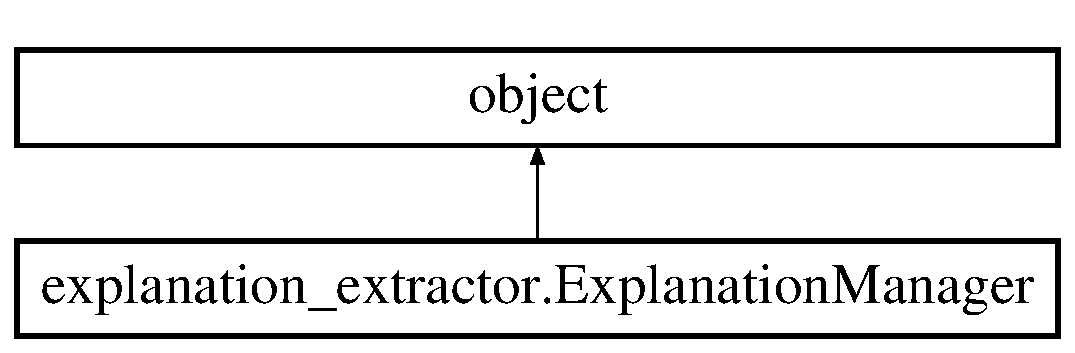
\includegraphics[height=2.000000cm]{classexplanation__extractor_1_1_explanation_manager}
\end{center}
\end{figure}
\subsection*{Public Member Functions}
\begin{DoxyCompactItemize}
\item 
def \hyperlink{classexplanation__extractor_1_1_explanation_manager_a200693544d5c773571a0c0068a428439}{\+\_\+\+\_\+init\+\_\+\+\_\+} (self)
\item 
def \hyperlink{classexplanation__extractor_1_1_explanation_manager_a595b2b449442a170122c2526a78ed3fd}{add\+Explanation\+Template} (self, rule)
\item 
def \hyperlink{classexplanation__extractor_1_1_explanation_manager_a11bc69dcaf562b5107f353692969ac25}{lookup\+Heuristic\+Key} (self, heur\+\_\+string)
\item 
def \hyperlink{classexplanation__extractor_1_1_explanation_manager_a13d8dadd73b2acfa1ad2b4ffee9c6d39}{lookup\+Template\+For} (self, predicate\+\_\+key)
\item 
def \hyperlink{classexplanation__extractor_1_1_explanation_manager_a42a90b38813341194d28bb718b62de83}{has\+Explanation\+For\+Predicate} (self, predicate)
\end{DoxyCompactItemize}
\subsection*{Static Public Member Functions}
\begin{DoxyCompactItemize}
\item 
def \hyperlink{classexplanation__extractor_1_1_explanation_manager_a04299eda21809209efe46537820daf41}{make\+Rule\+Key} (rule)
\item 
def \hyperlink{classexplanation__extractor_1_1_explanation_manager_ae4bf9fd7c6fe136b02d1700bcfff3f52}{make\+Pred\+Key} (predicate)
\end{DoxyCompactItemize}
\subsection*{Public Attributes}
\begin{DoxyCompactItemize}
\item 
\hyperlink{classexplanation__extractor_1_1_explanation_manager_a721b8077c8e3704a56e19de566f9dbda}{templates}
\item 
\hyperlink{classexplanation__extractor_1_1_explanation_manager_ad528733dbb33f6d033a3ee7738bfe91e}{heuristic\+\_\+to\+\_\+heur\+\_\+key}
\end{DoxyCompactItemize}


\subsection{Detailed Description}
\begin{DoxyVerb}manages a set of explanations extracted from ASP gringo files\end{DoxyVerb}
 

Definition at line 133 of file explanation\+\_\+extractor.\+py.



\subsection{Constructor \& Destructor Documentation}
\hypertarget{classexplanation__extractor_1_1_explanation_manager_a200693544d5c773571a0c0068a428439}{}\index{explanation\+\_\+extractor\+::\+Explanation\+Manager@{explanation\+\_\+extractor\+::\+Explanation\+Manager}!\+\_\+\+\_\+init\+\_\+\+\_\+@{\+\_\+\+\_\+init\+\_\+\+\_\+}}
\index{\+\_\+\+\_\+init\+\_\+\+\_\+@{\+\_\+\+\_\+init\+\_\+\+\_\+}!explanation\+\_\+extractor\+::\+Explanation\+Manager@{explanation\+\_\+extractor\+::\+Explanation\+Manager}}
\subsubsection[{\+\_\+\+\_\+init\+\_\+\+\_\+}]{\setlength{\rightskip}{0pt plus 5cm}def explanation\+\_\+extractor.\+Explanation\+Manager.\+\_\+\+\_\+init\+\_\+\+\_\+ (
\begin{DoxyParamCaption}
\item[{}]{self}
\end{DoxyParamCaption}
)}\label{classexplanation__extractor_1_1_explanation_manager_a200693544d5c773571a0c0068a428439}


Definition at line 135 of file explanation\+\_\+extractor.\+py.



\subsection{Member Function Documentation}
\hypertarget{classexplanation__extractor_1_1_explanation_manager_a595b2b449442a170122c2526a78ed3fd}{}\index{explanation\+\_\+extractor\+::\+Explanation\+Manager@{explanation\+\_\+extractor\+::\+Explanation\+Manager}!add\+Explanation\+Template@{add\+Explanation\+Template}}
\index{add\+Explanation\+Template@{add\+Explanation\+Template}!explanation\+\_\+extractor\+::\+Explanation\+Manager@{explanation\+\_\+extractor\+::\+Explanation\+Manager}}
\subsubsection[{add\+Explanation\+Template}]{\setlength{\rightskip}{0pt plus 5cm}def explanation\+\_\+extractor.\+Explanation\+Manager.\+add\+Explanation\+Template (
\begin{DoxyParamCaption}
\item[{}]{self, }
\item[{}]{rule}
\end{DoxyParamCaption}
)}\label{classexplanation__extractor_1_1_explanation_manager_a595b2b449442a170122c2526a78ed3fd}
\begin{DoxyVerb}instantiate new ExplanationTemplate instance for given predicate \end{DoxyVerb}
 

Definition at line 140 of file explanation\+\_\+extractor.\+py.

\hypertarget{classexplanation__extractor_1_1_explanation_manager_a42a90b38813341194d28bb718b62de83}{}\index{explanation\+\_\+extractor\+::\+Explanation\+Manager@{explanation\+\_\+extractor\+::\+Explanation\+Manager}!has\+Explanation\+For\+Predicate@{has\+Explanation\+For\+Predicate}}
\index{has\+Explanation\+For\+Predicate@{has\+Explanation\+For\+Predicate}!explanation\+\_\+extractor\+::\+Explanation\+Manager@{explanation\+\_\+extractor\+::\+Explanation\+Manager}}
\subsubsection[{has\+Explanation\+For\+Predicate}]{\setlength{\rightskip}{0pt plus 5cm}def explanation\+\_\+extractor.\+Explanation\+Manager.\+has\+Explanation\+For\+Predicate (
\begin{DoxyParamCaption}
\item[{}]{self, }
\item[{}]{predicate}
\end{DoxyParamCaption}
)}\label{classexplanation__extractor_1_1_explanation_manager_a42a90b38813341194d28bb718b62de83}


Definition at line 186 of file explanation\+\_\+extractor.\+py.

\hypertarget{classexplanation__extractor_1_1_explanation_manager_a11bc69dcaf562b5107f353692969ac25}{}\index{explanation\+\_\+extractor\+::\+Explanation\+Manager@{explanation\+\_\+extractor\+::\+Explanation\+Manager}!lookup\+Heuristic\+Key@{lookup\+Heuristic\+Key}}
\index{lookup\+Heuristic\+Key@{lookup\+Heuristic\+Key}!explanation\+\_\+extractor\+::\+Explanation\+Manager@{explanation\+\_\+extractor\+::\+Explanation\+Manager}}
\subsubsection[{lookup\+Heuristic\+Key}]{\setlength{\rightskip}{0pt plus 5cm}def explanation\+\_\+extractor.\+Explanation\+Manager.\+lookup\+Heuristic\+Key (
\begin{DoxyParamCaption}
\item[{}]{self, }
\item[{}]{heur\+\_\+string}
\end{DoxyParamCaption}
)}\label{classexplanation__extractor_1_1_explanation_manager_a11bc69dcaf562b5107f353692969ac25}


Definition at line 153 of file explanation\+\_\+extractor.\+py.

\hypertarget{classexplanation__extractor_1_1_explanation_manager_a13d8dadd73b2acfa1ad2b4ffee9c6d39}{}\index{explanation\+\_\+extractor\+::\+Explanation\+Manager@{explanation\+\_\+extractor\+::\+Explanation\+Manager}!lookup\+Template\+For@{lookup\+Template\+For}}
\index{lookup\+Template\+For@{lookup\+Template\+For}!explanation\+\_\+extractor\+::\+Explanation\+Manager@{explanation\+\_\+extractor\+::\+Explanation\+Manager}}
\subsubsection[{lookup\+Template\+For}]{\setlength{\rightskip}{0pt plus 5cm}def explanation\+\_\+extractor.\+Explanation\+Manager.\+lookup\+Template\+For (
\begin{DoxyParamCaption}
\item[{}]{self, }
\item[{}]{predicate\+\_\+key}
\end{DoxyParamCaption}
)}\label{classexplanation__extractor_1_1_explanation_manager_a13d8dadd73b2acfa1ad2b4ffee9c6d39}
\begin{DoxyVerb}Return an ExplanationTemplate instance for given predicate_key
predicate_ key = (predicate_name, arity)
NOTE: predicate_key  should be generated using ExplanationManager.makeRuleKey(rule) or makePredKey()
\end{DoxyVerb}
 

Definition at line 156 of file explanation\+\_\+extractor.\+py.

\hypertarget{classexplanation__extractor_1_1_explanation_manager_ae4bf9fd7c6fe136b02d1700bcfff3f52}{}\index{explanation\+\_\+extractor\+::\+Explanation\+Manager@{explanation\+\_\+extractor\+::\+Explanation\+Manager}!make\+Pred\+Key@{make\+Pred\+Key}}
\index{make\+Pred\+Key@{make\+Pred\+Key}!explanation\+\_\+extractor\+::\+Explanation\+Manager@{explanation\+\_\+extractor\+::\+Explanation\+Manager}}
\subsubsection[{make\+Pred\+Key}]{\setlength{\rightskip}{0pt plus 5cm}def explanation\+\_\+extractor.\+Explanation\+Manager.\+make\+Pred\+Key (
\begin{DoxyParamCaption}
\item[{}]{predicate}
\end{DoxyParamCaption}
)\hspace{0.3cm}{\ttfamily [static]}}\label{classexplanation__extractor_1_1_explanation_manager_ae4bf9fd7c6fe136b02d1700bcfff3f52}
\begin{DoxyVerb}heuristics have a key determined by condition and arity of their operands. Other predicates
are indexed by their own predicate name and arity\end{DoxyVerb}
 

Definition at line 172 of file explanation\+\_\+extractor.\+py.

\hypertarget{classexplanation__extractor_1_1_explanation_manager_a04299eda21809209efe46537820daf41}{}\index{explanation\+\_\+extractor\+::\+Explanation\+Manager@{explanation\+\_\+extractor\+::\+Explanation\+Manager}!make\+Rule\+Key@{make\+Rule\+Key}}
\index{make\+Rule\+Key@{make\+Rule\+Key}!explanation\+\_\+extractor\+::\+Explanation\+Manager@{explanation\+\_\+extractor\+::\+Explanation\+Manager}}
\subsubsection[{make\+Rule\+Key}]{\setlength{\rightskip}{0pt plus 5cm}def explanation\+\_\+extractor.\+Explanation\+Manager.\+make\+Rule\+Key (
\begin{DoxyParamCaption}
\item[{}]{rule}
\end{DoxyParamCaption}
)\hspace{0.3cm}{\ttfamily [static]}}\label{classexplanation__extractor_1_1_explanation_manager_a04299eda21809209efe46537820daf41}
\begin{DoxyVerb}return predicate key for given rule \end{DoxyVerb}
 

Definition at line 167 of file explanation\+\_\+extractor.\+py.



\subsection{Member Data Documentation}
\hypertarget{classexplanation__extractor_1_1_explanation_manager_ad528733dbb33f6d033a3ee7738bfe91e}{}\index{explanation\+\_\+extractor\+::\+Explanation\+Manager@{explanation\+\_\+extractor\+::\+Explanation\+Manager}!heuristic\+\_\+to\+\_\+heur\+\_\+key@{heuristic\+\_\+to\+\_\+heur\+\_\+key}}
\index{heuristic\+\_\+to\+\_\+heur\+\_\+key@{heuristic\+\_\+to\+\_\+heur\+\_\+key}!explanation\+\_\+extractor\+::\+Explanation\+Manager@{explanation\+\_\+extractor\+::\+Explanation\+Manager}}
\subsubsection[{heuristic\+\_\+to\+\_\+heur\+\_\+key}]{\setlength{\rightskip}{0pt plus 5cm}explanation\+\_\+extractor.\+Explanation\+Manager.\+heuristic\+\_\+to\+\_\+heur\+\_\+key}\label{classexplanation__extractor_1_1_explanation_manager_ad528733dbb33f6d033a3ee7738bfe91e}


Definition at line 138 of file explanation\+\_\+extractor.\+py.

\hypertarget{classexplanation__extractor_1_1_explanation_manager_a721b8077c8e3704a56e19de566f9dbda}{}\index{explanation\+\_\+extractor\+::\+Explanation\+Manager@{explanation\+\_\+extractor\+::\+Explanation\+Manager}!templates@{templates}}
\index{templates@{templates}!explanation\+\_\+extractor\+::\+Explanation\+Manager@{explanation\+\_\+extractor\+::\+Explanation\+Manager}}
\subsubsection[{templates}]{\setlength{\rightskip}{0pt plus 5cm}explanation\+\_\+extractor.\+Explanation\+Manager.\+templates}\label{classexplanation__extractor_1_1_explanation_manager_a721b8077c8e3704a56e19de566f9dbda}


Definition at line 137 of file explanation\+\_\+extractor.\+py.



The documentation for this class was generated from the following file\+:\begin{DoxyCompactItemize}
\item 
\hyperlink{explanation__extractor_8py}{explanation\+\_\+extractor.\+py}\end{DoxyCompactItemize}

\hypertarget{classexplanation__extractor_1_1_explanation_template}{}\section{explanation\+\_\+extractor.\+Explanation\+Template Class Reference}
\label{classexplanation__extractor_1_1_explanation_template}\index{explanation\+\_\+extractor.\+Explanation\+Template@{explanation\+\_\+extractor.\+Explanation\+Template}}
Inheritance diagram for explanation\+\_\+extractor.\+Explanation\+Template\+:\begin{figure}[H]
\begin{center}
\leavevmode
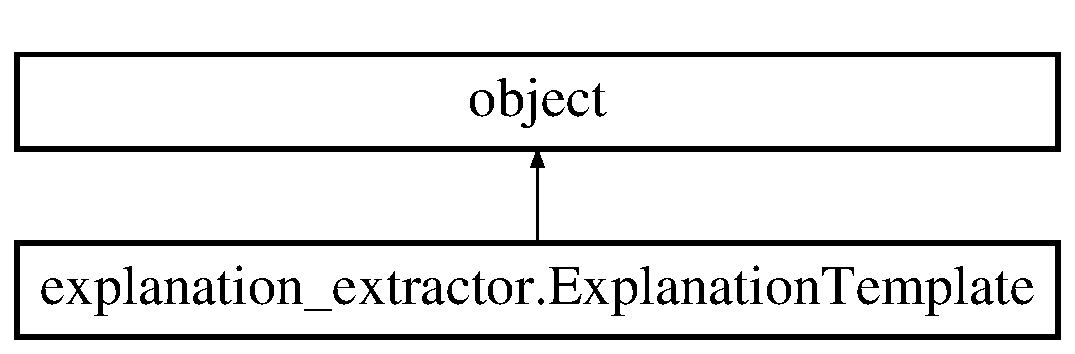
\includegraphics[height=2.000000cm]{classexplanation__extractor_1_1_explanation_template}
\end{center}
\end{figure}
\subsection*{Public Member Functions}
\begin{DoxyCompactItemize}
\item 
def \hyperlink{classexplanation__extractor_1_1_explanation_template_ae384db02e5b25f8a9da90b0554ea6459}{\+\_\+\+\_\+init\+\_\+\+\_\+} (self, \hyperlink{classexplanation__extractor_1_1_explanation_template_a4c4f2a6dd654e3aaa157970cc2c7bc21}{rule}, \hyperlink{classexplanation__extractor_1_1_explanation_template_a2f5ae7f61f258fd2d7d00aa9c21dcf39}{manager})
\item 
def \hyperlink{classexplanation__extractor_1_1_explanation_template_a1d4f9bb84ac2963aeea1208a8581f4a1}{add\+Additional\+Explanation} (self, \hyperlink{classexplanation__extractor_1_1_explanation_template_a4c4f2a6dd654e3aaa157970cc2c7bc21}{rule})
\item 
def \hyperlink{classexplanation__extractor_1_1_explanation_template_a6b8c95a94d1c6fc0abd092d70f6ac38a}{unify\+Vars} (self, var\+\_\+dictionary, model\+\_\+manager)
\item 
def \hyperlink{classexplanation__extractor_1_1_explanation_template_a4d5294a7b4df213aead6810020bcf5cf}{make\+Explanation}
\item 
def \hyperlink{classexplanation__extractor_1_1_explanation_template_a7de60c59f6bcb0557da1b1224efffca7}{make\+Head\+Explanation}
\item 
def \hyperlink{classexplanation__extractor_1_1_explanation_template_a86916fa50f74c7616a9f0cdb45cfe244}{unify\+And\+Make\+Body\+Explanation}
\item 
def \hyperlink{classexplanation__extractor_1_1_explanation_template_a0fbdf0b2b433f72519cecb10574e6049}{make\+Body\+Explanation}
\item 
def \hyperlink{classexplanation__extractor_1_1_explanation_template_aa64a3925b5b9ebc1f759b3eadc40df07}{pred\+List\+To\+Sentences} (self, pred\+\_\+list, var\+\_\+asignments, factor\+\_\+data)
\item 
def \hyperlink{classexplanation__extractor_1_1_explanation_template_a096ba3366ce13f3890f2329455c49908}{make\+Predicate\+Explanation}
\item 
def \hyperlink{classexplanation__extractor_1_1_explanation_template_a546a62509ffc27ffbb602dbd9a2c77b2}{splice\+In\+Factor\+Data} (self, raw\+\_\+predicate\+\_\+name, factor\+\_\+data)
\end{DoxyCompactItemize}
\subsection*{Static Public Member Functions}
\begin{DoxyCompactItemize}
\item 
def \hyperlink{classexplanation__extractor_1_1_explanation_template_a6dee7209b093a86ecc6b5bae18d458bc}{is\+Unified} (condition, var\+\_\+assignment)
\item 
def \hyperlink{classexplanation__extractor_1_1_explanation_template_a5d5da10c74e21a3038b128a3bcb3b9de}{substitute\+Variable\+Values} (var\+\_\+names, var\+\_\+assignment)
\item 
def \hyperlink{classexplanation__extractor_1_1_explanation_template_a9a57971dfdabe76fbc752548bcf095f4}{translate\+Vars\+To\+Template\+Names} (template, var\+\_\+assignment, old\+\_\+variables)
\item 
def \hyperlink{classexplanation__extractor_1_1_explanation_template_ad14ac7b106c4c8822678bd9bfbcf0b17}{unify} (var\+\_\+assignment, conditions, model\+\_\+mgr)
\item 
def \hyperlink{classexplanation__extractor_1_1_explanation_template_a47d50adeccec8141590eb51a9694219f}{get\+Predicate\+Variables} (predicate)
\end{DoxyCompactItemize}
\subsection*{Public Attributes}
\begin{DoxyCompactItemize}
\item 
\hyperlink{classexplanation__extractor_1_1_explanation_template_a4c4f2a6dd654e3aaa157970cc2c7bc21}{rule}
\item 
\hyperlink{classexplanation__extractor_1_1_explanation_template_a2f5ae7f61f258fd2d7d00aa9c21dcf39}{manager}
\end{DoxyCompactItemize}


\subsection{Detailed Description}
\begin{DoxyVerb}stores the explanation logic for a single predicate type. A predicate type
is defined by both predicate name and arity.\end{DoxyVerb}
 

Definition at line 190 of file explanation\+\_\+extractor.\+py.



\subsection{Constructor \& Destructor Documentation}
\hypertarget{classexplanation__extractor_1_1_explanation_template_ae384db02e5b25f8a9da90b0554ea6459}{}\index{explanation\+\_\+extractor\+::\+Explanation\+Template@{explanation\+\_\+extractor\+::\+Explanation\+Template}!\+\_\+\+\_\+init\+\_\+\+\_\+@{\+\_\+\+\_\+init\+\_\+\+\_\+}}
\index{\+\_\+\+\_\+init\+\_\+\+\_\+@{\+\_\+\+\_\+init\+\_\+\+\_\+}!explanation\+\_\+extractor\+::\+Explanation\+Template@{explanation\+\_\+extractor\+::\+Explanation\+Template}}
\subsubsection[{\+\_\+\+\_\+init\+\_\+\+\_\+}]{\setlength{\rightskip}{0pt plus 5cm}def explanation\+\_\+extractor.\+Explanation\+Template.\+\_\+\+\_\+init\+\_\+\+\_\+ (
\begin{DoxyParamCaption}
\item[{}]{self, }
\item[{}]{rule, }
\item[{}]{manager}
\end{DoxyParamCaption}
)}\label{classexplanation__extractor_1_1_explanation_template_ae384db02e5b25f8a9da90b0554ea6459}


Definition at line 193 of file explanation\+\_\+extractor.\+py.



\subsection{Member Function Documentation}
\hypertarget{classexplanation__extractor_1_1_explanation_template_a1d4f9bb84ac2963aeea1208a8581f4a1}{}\index{explanation\+\_\+extractor\+::\+Explanation\+Template@{explanation\+\_\+extractor\+::\+Explanation\+Template}!add\+Additional\+Explanation@{add\+Additional\+Explanation}}
\index{add\+Additional\+Explanation@{add\+Additional\+Explanation}!explanation\+\_\+extractor\+::\+Explanation\+Template@{explanation\+\_\+extractor\+::\+Explanation\+Template}}
\subsubsection[{add\+Additional\+Explanation}]{\setlength{\rightskip}{0pt plus 5cm}def explanation\+\_\+extractor.\+Explanation\+Template.\+add\+Additional\+Explanation (
\begin{DoxyParamCaption}
\item[{}]{self, }
\item[{}]{rule}
\end{DoxyParamCaption}
)}\label{classexplanation__extractor_1_1_explanation_template_a1d4f9bb84ac2963aeea1208a8581f4a1}
\begin{DoxyVerb}Some predicates can be derived in more than one way\end{DoxyVerb}
 

Definition at line 198 of file explanation\+\_\+extractor.\+py.

\hypertarget{classexplanation__extractor_1_1_explanation_template_a47d50adeccec8141590eb51a9694219f}{}\index{explanation\+\_\+extractor\+::\+Explanation\+Template@{explanation\+\_\+extractor\+::\+Explanation\+Template}!get\+Predicate\+Variables@{get\+Predicate\+Variables}}
\index{get\+Predicate\+Variables@{get\+Predicate\+Variables}!explanation\+\_\+extractor\+::\+Explanation\+Template@{explanation\+\_\+extractor\+::\+Explanation\+Template}}
\subsubsection[{get\+Predicate\+Variables}]{\setlength{\rightskip}{0pt plus 5cm}def explanation\+\_\+extractor.\+Explanation\+Template.\+get\+Predicate\+Variables (
\begin{DoxyParamCaption}
\item[{}]{predicate}
\end{DoxyParamCaption}
)\hspace{0.3cm}{\ttfamily [static]}}\label{classexplanation__extractor_1_1_explanation_template_a47d50adeccec8141590eb51a9694219f}
\begin{DoxyVerb}return a list of variables referenced by given predicate\end{DoxyVerb}
 

Definition at line 312 of file explanation\+\_\+extractor.\+py.

\hypertarget{classexplanation__extractor_1_1_explanation_template_a6dee7209b093a86ecc6b5bae18d458bc}{}\index{explanation\+\_\+extractor\+::\+Explanation\+Template@{explanation\+\_\+extractor\+::\+Explanation\+Template}!is\+Unified@{is\+Unified}}
\index{is\+Unified@{is\+Unified}!explanation\+\_\+extractor\+::\+Explanation\+Template@{explanation\+\_\+extractor\+::\+Explanation\+Template}}
\subsubsection[{is\+Unified}]{\setlength{\rightskip}{0pt plus 5cm}def explanation\+\_\+extractor.\+Explanation\+Template.\+is\+Unified (
\begin{DoxyParamCaption}
\item[{}]{condition, }
\item[{}]{var\+\_\+assignment}
\end{DoxyParamCaption}
)\hspace{0.3cm}{\ttfamily [static]}}\label{classexplanation__extractor_1_1_explanation_template_a6dee7209b093a86ecc6b5bae18d458bc}


Definition at line 203 of file explanation\+\_\+extractor.\+py.

\hypertarget{classexplanation__extractor_1_1_explanation_template_a0fbdf0b2b433f72519cecb10574e6049}{}\index{explanation\+\_\+extractor\+::\+Explanation\+Template@{explanation\+\_\+extractor\+::\+Explanation\+Template}!make\+Body\+Explanation@{make\+Body\+Explanation}}
\index{make\+Body\+Explanation@{make\+Body\+Explanation}!explanation\+\_\+extractor\+::\+Explanation\+Template@{explanation\+\_\+extractor\+::\+Explanation\+Template}}
\subsubsection[{make\+Body\+Explanation}]{\setlength{\rightskip}{0pt plus 5cm}def explanation\+\_\+extractor.\+Explanation\+Template.\+make\+Body\+Explanation (
\begin{DoxyParamCaption}
\item[{}]{self, }
\item[{}]{var\+\_\+assignments, }
\item[{}]{model\+\_\+manager = {\ttfamily None}, }
\item[{}]{depth = {\ttfamily 1}, }
\item[{}]{factor\+\_\+data = {\ttfamily \{\}}}
\end{DoxyParamCaption}
)}\label{classexplanation__extractor_1_1_explanation_template_a0fbdf0b2b433f72519cecb10574e6049}


Definition at line 290 of file explanation\+\_\+extractor.\+py.

\hypertarget{classexplanation__extractor_1_1_explanation_template_a4d5294a7b4df213aead6810020bcf5cf}{}\index{explanation\+\_\+extractor\+::\+Explanation\+Template@{explanation\+\_\+extractor\+::\+Explanation\+Template}!make\+Explanation@{make\+Explanation}}
\index{make\+Explanation@{make\+Explanation}!explanation\+\_\+extractor\+::\+Explanation\+Template@{explanation\+\_\+extractor\+::\+Explanation\+Template}}
\subsubsection[{make\+Explanation}]{\setlength{\rightskip}{0pt plus 5cm}def explanation\+\_\+extractor.\+Explanation\+Template.\+make\+Explanation (
\begin{DoxyParamCaption}
\item[{}]{self, }
\item[{}]{var\+\_\+values, }
\item[{}]{model\+\_\+manager = {\ttfamily None}, }
\item[{}]{depth = {\ttfamily 1}, }
\item[{}]{factor\+\_\+data = {\ttfamily \{\}}}
\end{DoxyParamCaption}
)}\label{classexplanation__extractor_1_1_explanation_template_a4d5294a7b4df213aead6810020bcf5cf}
\begin{DoxyVerb}return list of template sentences containing explanation\end{DoxyVerb}
 

Definition at line 265 of file explanation\+\_\+extractor.\+py.

\hypertarget{classexplanation__extractor_1_1_explanation_template_a7de60c59f6bcb0557da1b1224efffca7}{}\index{explanation\+\_\+extractor\+::\+Explanation\+Template@{explanation\+\_\+extractor\+::\+Explanation\+Template}!make\+Head\+Explanation@{make\+Head\+Explanation}}
\index{make\+Head\+Explanation@{make\+Head\+Explanation}!explanation\+\_\+extractor\+::\+Explanation\+Template@{explanation\+\_\+extractor\+::\+Explanation\+Template}}
\subsubsection[{make\+Head\+Explanation}]{\setlength{\rightskip}{0pt plus 5cm}def explanation\+\_\+extractor.\+Explanation\+Template.\+make\+Head\+Explanation (
\begin{DoxyParamCaption}
\item[{}]{self, }
\item[{}]{var\+\_\+assignments, }
\item[{}]{factor\+\_\+data = {\ttfamily \{\}}}
\end{DoxyParamCaption}
)}\label{classexplanation__extractor_1_1_explanation_template_a7de60c59f6bcb0557da1b1224efffca7}


Definition at line 275 of file explanation\+\_\+extractor.\+py.

\hypertarget{classexplanation__extractor_1_1_explanation_template_a096ba3366ce13f3890f2329455c49908}{}\index{explanation\+\_\+extractor\+::\+Explanation\+Template@{explanation\+\_\+extractor\+::\+Explanation\+Template}!make\+Predicate\+Explanation@{make\+Predicate\+Explanation}}
\index{make\+Predicate\+Explanation@{make\+Predicate\+Explanation}!explanation\+\_\+extractor\+::\+Explanation\+Template@{explanation\+\_\+extractor\+::\+Explanation\+Template}}
\subsubsection[{make\+Predicate\+Explanation}]{\setlength{\rightskip}{0pt plus 5cm}def explanation\+\_\+extractor.\+Explanation\+Template.\+make\+Predicate\+Explanation (
\begin{DoxyParamCaption}
\item[{}]{self, }
\item[{}]{predicate, }
\item[{}]{var\+\_\+assignments, }
\item[{}]{factor\+\_\+data = {\ttfamily \{\}}}
\end{DoxyParamCaption}
)}\label{classexplanation__extractor_1_1_explanation_template_a096ba3366ce13f3890f2329455c49908}


Definition at line 321 of file explanation\+\_\+extractor.\+py.

\hypertarget{classexplanation__extractor_1_1_explanation_template_aa64a3925b5b9ebc1f759b3eadc40df07}{}\index{explanation\+\_\+extractor\+::\+Explanation\+Template@{explanation\+\_\+extractor\+::\+Explanation\+Template}!pred\+List\+To\+Sentences@{pred\+List\+To\+Sentences}}
\index{pred\+List\+To\+Sentences@{pred\+List\+To\+Sentences}!explanation\+\_\+extractor\+::\+Explanation\+Template@{explanation\+\_\+extractor\+::\+Explanation\+Template}}
\subsubsection[{pred\+List\+To\+Sentences}]{\setlength{\rightskip}{0pt plus 5cm}def explanation\+\_\+extractor.\+Explanation\+Template.\+pred\+List\+To\+Sentences (
\begin{DoxyParamCaption}
\item[{}]{self, }
\item[{}]{pred\+\_\+list, }
\item[{}]{var\+\_\+asignments, }
\item[{}]{factor\+\_\+data}
\end{DoxyParamCaption}
)}\label{classexplanation__extractor_1_1_explanation_template_aa64a3925b5b9ebc1f759b3eadc40df07}


Definition at line 309 of file explanation\+\_\+extractor.\+py.

\hypertarget{classexplanation__extractor_1_1_explanation_template_a546a62509ffc27ffbb602dbd9a2c77b2}{}\index{explanation\+\_\+extractor\+::\+Explanation\+Template@{explanation\+\_\+extractor\+::\+Explanation\+Template}!splice\+In\+Factor\+Data@{splice\+In\+Factor\+Data}}
\index{splice\+In\+Factor\+Data@{splice\+In\+Factor\+Data}!explanation\+\_\+extractor\+::\+Explanation\+Template@{explanation\+\_\+extractor\+::\+Explanation\+Template}}
\subsubsection[{splice\+In\+Factor\+Data}]{\setlength{\rightskip}{0pt plus 5cm}def explanation\+\_\+extractor.\+Explanation\+Template.\+splice\+In\+Factor\+Data (
\begin{DoxyParamCaption}
\item[{}]{self, }
\item[{}]{raw\+\_\+predicate\+\_\+name, }
\item[{}]{factor\+\_\+data}
\end{DoxyParamCaption}
)}\label{classexplanation__extractor_1_1_explanation_template_a546a62509ffc27ffbb602dbd9a2c77b2}


Definition at line 325 of file explanation\+\_\+extractor.\+py.

\hypertarget{classexplanation__extractor_1_1_explanation_template_a5d5da10c74e21a3038b128a3bcb3b9de}{}\index{explanation\+\_\+extractor\+::\+Explanation\+Template@{explanation\+\_\+extractor\+::\+Explanation\+Template}!substitute\+Variable\+Values@{substitute\+Variable\+Values}}
\index{substitute\+Variable\+Values@{substitute\+Variable\+Values}!explanation\+\_\+extractor\+::\+Explanation\+Template@{explanation\+\_\+extractor\+::\+Explanation\+Template}}
\subsubsection[{substitute\+Variable\+Values}]{\setlength{\rightskip}{0pt plus 5cm}def explanation\+\_\+extractor.\+Explanation\+Template.\+substitute\+Variable\+Values (
\begin{DoxyParamCaption}
\item[{}]{var\+\_\+names, }
\item[{}]{var\+\_\+assignment}
\end{DoxyParamCaption}
)\hspace{0.3cm}{\ttfamily [static]}}\label{classexplanation__extractor_1_1_explanation_template_a5d5da10c74e21a3038b128a3bcb3b9de}


Definition at line 209 of file explanation\+\_\+extractor.\+py.

\hypertarget{classexplanation__extractor_1_1_explanation_template_a9a57971dfdabe76fbc752548bcf095f4}{}\index{explanation\+\_\+extractor\+::\+Explanation\+Template@{explanation\+\_\+extractor\+::\+Explanation\+Template}!translate\+Vars\+To\+Template\+Names@{translate\+Vars\+To\+Template\+Names}}
\index{translate\+Vars\+To\+Template\+Names@{translate\+Vars\+To\+Template\+Names}!explanation\+\_\+extractor\+::\+Explanation\+Template@{explanation\+\_\+extractor\+::\+Explanation\+Template}}
\subsubsection[{translate\+Vars\+To\+Template\+Names}]{\setlength{\rightskip}{0pt plus 5cm}def explanation\+\_\+extractor.\+Explanation\+Template.\+translate\+Vars\+To\+Template\+Names (
\begin{DoxyParamCaption}
\item[{}]{template, }
\item[{}]{var\+\_\+assignment, }
\item[{}]{old\+\_\+variables}
\end{DoxyParamCaption}
)\hspace{0.3cm}{\ttfamily [static]}}\label{classexplanation__extractor_1_1_explanation_template_a9a57971dfdabe76fbc752548bcf095f4}


Definition at line 221 of file explanation\+\_\+extractor.\+py.

\hypertarget{classexplanation__extractor_1_1_explanation_template_ad14ac7b106c4c8822678bd9bfbcf0b17}{}\index{explanation\+\_\+extractor\+::\+Explanation\+Template@{explanation\+\_\+extractor\+::\+Explanation\+Template}!unify@{unify}}
\index{unify@{unify}!explanation\+\_\+extractor\+::\+Explanation\+Template@{explanation\+\_\+extractor\+::\+Explanation\+Template}}
\subsubsection[{unify}]{\setlength{\rightskip}{0pt plus 5cm}def explanation\+\_\+extractor.\+Explanation\+Template.\+unify (
\begin{DoxyParamCaption}
\item[{}]{var\+\_\+assignment, }
\item[{}]{conditions, }
\item[{}]{model\+\_\+mgr}
\end{DoxyParamCaption}
)\hspace{0.3cm}{\ttfamily [static]}}\label{classexplanation__extractor_1_1_explanation_template_ad14ac7b106c4c8822678bd9bfbcf0b17}


Definition at line 233 of file explanation\+\_\+extractor.\+py.

\hypertarget{classexplanation__extractor_1_1_explanation_template_a86916fa50f74c7616a9f0cdb45cfe244}{}\index{explanation\+\_\+extractor\+::\+Explanation\+Template@{explanation\+\_\+extractor\+::\+Explanation\+Template}!unify\+And\+Make\+Body\+Explanation@{unify\+And\+Make\+Body\+Explanation}}
\index{unify\+And\+Make\+Body\+Explanation@{unify\+And\+Make\+Body\+Explanation}!explanation\+\_\+extractor\+::\+Explanation\+Template@{explanation\+\_\+extractor\+::\+Explanation\+Template}}
\subsubsection[{unify\+And\+Make\+Body\+Explanation}]{\setlength{\rightskip}{0pt plus 5cm}def explanation\+\_\+extractor.\+Explanation\+Template.\+unify\+And\+Make\+Body\+Explanation (
\begin{DoxyParamCaption}
\item[{}]{self, }
\item[{}]{var\+\_\+assignments, }
\item[{}]{model\+\_\+manager = {\ttfamily None}, }
\item[{}]{depth = {\ttfamily 1}, }
\item[{}]{factor\+\_\+data = {\ttfamily \{\}}}
\end{DoxyParamCaption}
)}\label{classexplanation__extractor_1_1_explanation_template_a86916fa50f74c7616a9f0cdb45cfe244}


Definition at line 284 of file explanation\+\_\+extractor.\+py.

\hypertarget{classexplanation__extractor_1_1_explanation_template_a6b8c95a94d1c6fc0abd092d70f6ac38a}{}\index{explanation\+\_\+extractor\+::\+Explanation\+Template@{explanation\+\_\+extractor\+::\+Explanation\+Template}!unify\+Vars@{unify\+Vars}}
\index{unify\+Vars@{unify\+Vars}!explanation\+\_\+extractor\+::\+Explanation\+Template@{explanation\+\_\+extractor\+::\+Explanation\+Template}}
\subsubsection[{unify\+Vars}]{\setlength{\rightskip}{0pt plus 5cm}def explanation\+\_\+extractor.\+Explanation\+Template.\+unify\+Vars (
\begin{DoxyParamCaption}
\item[{}]{self, }
\item[{}]{var\+\_\+dictionary, }
\item[{}]{model\+\_\+manager}
\end{DoxyParamCaption}
)}\label{classexplanation__extractor_1_1_explanation_template_a6b8c95a94d1c6fc0abd092d70f6ac38a}


Definition at line 260 of file explanation\+\_\+extractor.\+py.



\subsection{Member Data Documentation}
\hypertarget{classexplanation__extractor_1_1_explanation_template_a2f5ae7f61f258fd2d7d00aa9c21dcf39}{}\index{explanation\+\_\+extractor\+::\+Explanation\+Template@{explanation\+\_\+extractor\+::\+Explanation\+Template}!manager@{manager}}
\index{manager@{manager}!explanation\+\_\+extractor\+::\+Explanation\+Template@{explanation\+\_\+extractor\+::\+Explanation\+Template}}
\subsubsection[{manager}]{\setlength{\rightskip}{0pt plus 5cm}explanation\+\_\+extractor.\+Explanation\+Template.\+manager}\label{classexplanation__extractor_1_1_explanation_template_a2f5ae7f61f258fd2d7d00aa9c21dcf39}


Definition at line 196 of file explanation\+\_\+extractor.\+py.

\hypertarget{classexplanation__extractor_1_1_explanation_template_a4c4f2a6dd654e3aaa157970cc2c7bc21}{}\index{explanation\+\_\+extractor\+::\+Explanation\+Template@{explanation\+\_\+extractor\+::\+Explanation\+Template}!rule@{rule}}
\index{rule@{rule}!explanation\+\_\+extractor\+::\+Explanation\+Template@{explanation\+\_\+extractor\+::\+Explanation\+Template}}
\subsubsection[{rule}]{\setlength{\rightskip}{0pt plus 5cm}explanation\+\_\+extractor.\+Explanation\+Template.\+rule}\label{classexplanation__extractor_1_1_explanation_template_a4c4f2a6dd654e3aaa157970cc2c7bc21}


Definition at line 195 of file explanation\+\_\+extractor.\+py.



The documentation for this class was generated from the following file\+:\begin{DoxyCompactItemize}
\item 
\hyperlink{explanation__extractor_8py}{explanation\+\_\+extractor.\+py}\end{DoxyCompactItemize}

\hypertarget{class_prolog_rules_parser_1_1_prolog_rules_parser_1_1_fact_context}{}\section{Prolog\+Rules\+Parser.\+Prolog\+Rules\+Parser.\+Fact\+Context Class Reference}
\label{class_prolog_rules_parser_1_1_prolog_rules_parser_1_1_fact_context}\index{Prolog\+Rules\+Parser.\+Prolog\+Rules\+Parser.\+Fact\+Context@{Prolog\+Rules\+Parser.\+Prolog\+Rules\+Parser.\+Fact\+Context}}
Inheritance diagram for Prolog\+Rules\+Parser.\+Prolog\+Rules\+Parser.\+Fact\+Context\+:\begin{figure}[H]
\begin{center}
\leavevmode
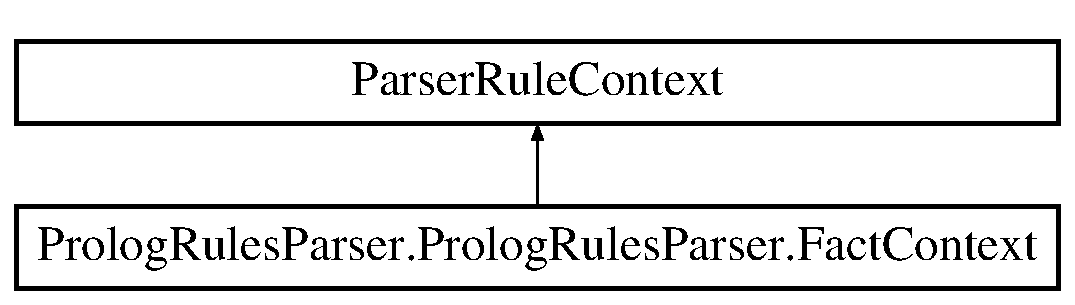
\includegraphics[height=2.000000cm]{class_prolog_rules_parser_1_1_prolog_rules_parser_1_1_fact_context}
\end{center}
\end{figure}
\subsection*{Public Member Functions}
\begin{DoxyCompactItemize}
\item 
def \hyperlink{class_prolog_rules_parser_1_1_prolog_rules_parser_1_1_fact_context_acf8b76fd5569948a2c528a6f7dbcacd2}{\+\_\+\+\_\+init\+\_\+\+\_\+}
\item 
def \hyperlink{class_prolog_rules_parser_1_1_prolog_rules_parser_1_1_fact_context_a1ac1cf4e8526cae0a1f5bc9c7e47a715}{predicate} (self)
\item 
def \hyperlink{class_prolog_rules_parser_1_1_prolog_rules_parser_1_1_fact_context_a008eb2cbf6d688744f8884fca5bccae4}{get\+Rule\+Index} (self)
\item 
def \hyperlink{class_prolog_rules_parser_1_1_prolog_rules_parser_1_1_fact_context_a9880eea916c1d066016a965f42618a5c}{enter\+Rule} (self, listener)
\item 
def \hyperlink{class_prolog_rules_parser_1_1_prolog_rules_parser_1_1_fact_context_a0a11cc822276f360dca79a80ad0830f9}{exit\+Rule} (self, listener)
\end{DoxyCompactItemize}
\subsection*{Public Attributes}
\begin{DoxyCompactItemize}
\item 
\hyperlink{class_prolog_rules_parser_1_1_prolog_rules_parser_1_1_fact_context_acd51a0725334ef43f7bcfc14f307011c}{parser}
\end{DoxyCompactItemize}


\subsection{Detailed Description}


Definition at line 255 of file Prolog\+Rules\+Parser.\+py.



\subsection{Constructor \& Destructor Documentation}
\hypertarget{class_prolog_rules_parser_1_1_prolog_rules_parser_1_1_fact_context_acf8b76fd5569948a2c528a6f7dbcacd2}{}\index{Prolog\+Rules\+Parser\+::\+Prolog\+Rules\+Parser\+::\+Fact\+Context@{Prolog\+Rules\+Parser\+::\+Prolog\+Rules\+Parser\+::\+Fact\+Context}!\+\_\+\+\_\+init\+\_\+\+\_\+@{\+\_\+\+\_\+init\+\_\+\+\_\+}}
\index{\+\_\+\+\_\+init\+\_\+\+\_\+@{\+\_\+\+\_\+init\+\_\+\+\_\+}!Prolog\+Rules\+Parser\+::\+Prolog\+Rules\+Parser\+::\+Fact\+Context@{Prolog\+Rules\+Parser\+::\+Prolog\+Rules\+Parser\+::\+Fact\+Context}}
\subsubsection[{\+\_\+\+\_\+init\+\_\+\+\_\+}]{\setlength{\rightskip}{0pt plus 5cm}def Prolog\+Rules\+Parser.\+Prolog\+Rules\+Parser.\+Fact\+Context.\+\_\+\+\_\+init\+\_\+\+\_\+ (
\begin{DoxyParamCaption}
\item[{}]{self, }
\item[{}]{parser, }
\item[{}]{parent = {\ttfamily None}, }
\item[{}]{invoking\+State = {\ttfamily -\/1}}
\end{DoxyParamCaption}
)}\label{class_prolog_rules_parser_1_1_prolog_rules_parser_1_1_fact_context_acf8b76fd5569948a2c528a6f7dbcacd2}


Definition at line 257 of file Prolog\+Rules\+Parser.\+py.



\subsection{Member Function Documentation}
\hypertarget{class_prolog_rules_parser_1_1_prolog_rules_parser_1_1_fact_context_a9880eea916c1d066016a965f42618a5c}{}\index{Prolog\+Rules\+Parser\+::\+Prolog\+Rules\+Parser\+::\+Fact\+Context@{Prolog\+Rules\+Parser\+::\+Prolog\+Rules\+Parser\+::\+Fact\+Context}!enter\+Rule@{enter\+Rule}}
\index{enter\+Rule@{enter\+Rule}!Prolog\+Rules\+Parser\+::\+Prolog\+Rules\+Parser\+::\+Fact\+Context@{Prolog\+Rules\+Parser\+::\+Prolog\+Rules\+Parser\+::\+Fact\+Context}}
\subsubsection[{enter\+Rule}]{\setlength{\rightskip}{0pt plus 5cm}def Prolog\+Rules\+Parser.\+Prolog\+Rules\+Parser.\+Fact\+Context.\+enter\+Rule (
\begin{DoxyParamCaption}
\item[{}]{self, }
\item[{}]{listener}
\end{DoxyParamCaption}
)}\label{class_prolog_rules_parser_1_1_prolog_rules_parser_1_1_fact_context_a9880eea916c1d066016a965f42618a5c}


Definition at line 268 of file Prolog\+Rules\+Parser.\+py.

\hypertarget{class_prolog_rules_parser_1_1_prolog_rules_parser_1_1_fact_context_a0a11cc822276f360dca79a80ad0830f9}{}\index{Prolog\+Rules\+Parser\+::\+Prolog\+Rules\+Parser\+::\+Fact\+Context@{Prolog\+Rules\+Parser\+::\+Prolog\+Rules\+Parser\+::\+Fact\+Context}!exit\+Rule@{exit\+Rule}}
\index{exit\+Rule@{exit\+Rule}!Prolog\+Rules\+Parser\+::\+Prolog\+Rules\+Parser\+::\+Fact\+Context@{Prolog\+Rules\+Parser\+::\+Prolog\+Rules\+Parser\+::\+Fact\+Context}}
\subsubsection[{exit\+Rule}]{\setlength{\rightskip}{0pt plus 5cm}def Prolog\+Rules\+Parser.\+Prolog\+Rules\+Parser.\+Fact\+Context.\+exit\+Rule (
\begin{DoxyParamCaption}
\item[{}]{self, }
\item[{}]{listener}
\end{DoxyParamCaption}
)}\label{class_prolog_rules_parser_1_1_prolog_rules_parser_1_1_fact_context_a0a11cc822276f360dca79a80ad0830f9}


Definition at line 272 of file Prolog\+Rules\+Parser.\+py.

\hypertarget{class_prolog_rules_parser_1_1_prolog_rules_parser_1_1_fact_context_a008eb2cbf6d688744f8884fca5bccae4}{}\index{Prolog\+Rules\+Parser\+::\+Prolog\+Rules\+Parser\+::\+Fact\+Context@{Prolog\+Rules\+Parser\+::\+Prolog\+Rules\+Parser\+::\+Fact\+Context}!get\+Rule\+Index@{get\+Rule\+Index}}
\index{get\+Rule\+Index@{get\+Rule\+Index}!Prolog\+Rules\+Parser\+::\+Prolog\+Rules\+Parser\+::\+Fact\+Context@{Prolog\+Rules\+Parser\+::\+Prolog\+Rules\+Parser\+::\+Fact\+Context}}
\subsubsection[{get\+Rule\+Index}]{\setlength{\rightskip}{0pt plus 5cm}def Prolog\+Rules\+Parser.\+Prolog\+Rules\+Parser.\+Fact\+Context.\+get\+Rule\+Index (
\begin{DoxyParamCaption}
\item[{}]{self}
\end{DoxyParamCaption}
)}\label{class_prolog_rules_parser_1_1_prolog_rules_parser_1_1_fact_context_a008eb2cbf6d688744f8884fca5bccae4}


Definition at line 265 of file Prolog\+Rules\+Parser.\+py.

\hypertarget{class_prolog_rules_parser_1_1_prolog_rules_parser_1_1_fact_context_a1ac1cf4e8526cae0a1f5bc9c7e47a715}{}\index{Prolog\+Rules\+Parser\+::\+Prolog\+Rules\+Parser\+::\+Fact\+Context@{Prolog\+Rules\+Parser\+::\+Prolog\+Rules\+Parser\+::\+Fact\+Context}!predicate@{predicate}}
\index{predicate@{predicate}!Prolog\+Rules\+Parser\+::\+Prolog\+Rules\+Parser\+::\+Fact\+Context@{Prolog\+Rules\+Parser\+::\+Prolog\+Rules\+Parser\+::\+Fact\+Context}}
\subsubsection[{predicate}]{\setlength{\rightskip}{0pt plus 5cm}def Prolog\+Rules\+Parser.\+Prolog\+Rules\+Parser.\+Fact\+Context.\+predicate (
\begin{DoxyParamCaption}
\item[{}]{self}
\end{DoxyParamCaption}
)}\label{class_prolog_rules_parser_1_1_prolog_rules_parser_1_1_fact_context_a1ac1cf4e8526cae0a1f5bc9c7e47a715}


Definition at line 261 of file Prolog\+Rules\+Parser.\+py.



\subsection{Member Data Documentation}
\hypertarget{class_prolog_rules_parser_1_1_prolog_rules_parser_1_1_fact_context_acd51a0725334ef43f7bcfc14f307011c}{}\index{Prolog\+Rules\+Parser\+::\+Prolog\+Rules\+Parser\+::\+Fact\+Context@{Prolog\+Rules\+Parser\+::\+Prolog\+Rules\+Parser\+::\+Fact\+Context}!parser@{parser}}
\index{parser@{parser}!Prolog\+Rules\+Parser\+::\+Prolog\+Rules\+Parser\+::\+Fact\+Context@{Prolog\+Rules\+Parser\+::\+Prolog\+Rules\+Parser\+::\+Fact\+Context}}
\subsubsection[{parser}]{\setlength{\rightskip}{0pt plus 5cm}Prolog\+Rules\+Parser.\+Prolog\+Rules\+Parser.\+Fact\+Context.\+parser}\label{class_prolog_rules_parser_1_1_prolog_rules_parser_1_1_fact_context_acd51a0725334ef43f7bcfc14f307011c}


Definition at line 259 of file Prolog\+Rules\+Parser.\+py.



The documentation for this class was generated from the following file\+:\begin{DoxyCompactItemize}
\item 
\hyperlink{_prolog_rules_parser_8py}{Prolog\+Rules\+Parser.\+py}\end{DoxyCompactItemize}

\hypertarget{classeqn__viz_1_1_generated_answer_set}{}\section{eqn\+\_\+viz.\+Generated\+Answer\+Set Class Reference}
\label{classeqn__viz_1_1_generated_answer_set}\index{eqn\+\_\+viz.\+Generated\+Answer\+Set@{eqn\+\_\+viz.\+Generated\+Answer\+Set}}
Inheritance diagram for eqn\+\_\+viz.\+Generated\+Answer\+Set\+:\begin{figure}[H]
\begin{center}
\leavevmode
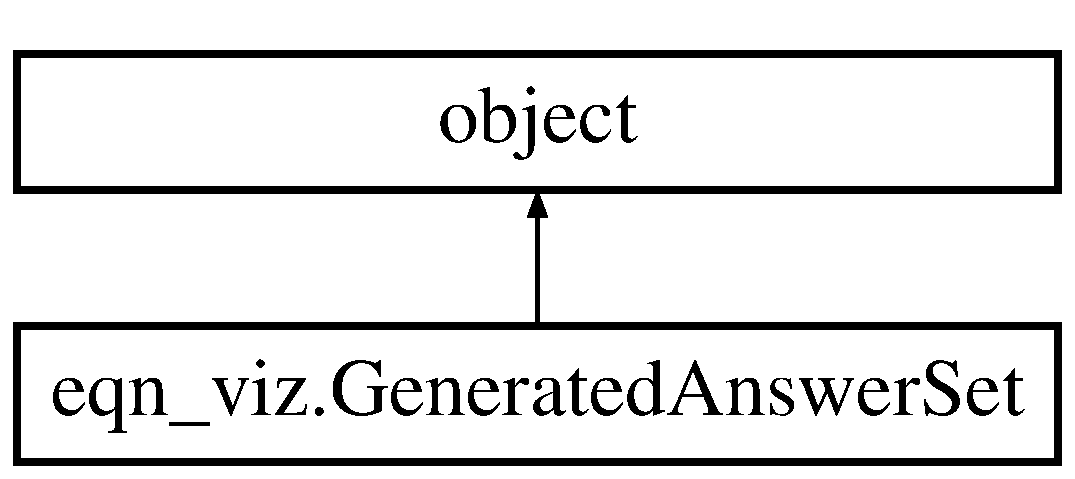
\includegraphics[height=2.000000cm]{classeqn__viz_1_1_generated_answer_set}
\end{center}
\end{figure}
\subsection*{Public Member Functions}
\begin{DoxyCompactItemize}
\item 
def \hyperlink{classeqn__viz_1_1_generated_answer_set_a3c05f96507e0e04c357e5bb5258d73fb}{\+\_\+\+\_\+init\+\_\+\+\_\+} (self, generated\+\_\+problems)
\item 
def \hyperlink{classeqn__viz_1_1_generated_answer_set_af10cd308ec2cceff4527854bea5fabb0}{get\+Math\+Problems} (self)
\item 
def \hyperlink{classeqn__viz_1_1_generated_answer_set_af0dde3d37bfb33361cb67db1cb7ba452}{to\+J\+S\+O\+N\+Format} (self)
\end{DoxyCompactItemize}
\subsection*{Public Attributes}
\begin{DoxyCompactItemize}
\item 
\hyperlink{classeqn__viz_1_1_generated_answer_set_acbdcff75642ae1eab5a35c6bb29a2a21}{generated\+\_\+problems\+\_\+dict}
\end{DoxyCompactItemize}


\subsection{Detailed Description}


Definition at line 121 of file eqn\+\_\+viz.\+py.



\subsection{Constructor \& Destructor Documentation}
\hypertarget{classeqn__viz_1_1_generated_answer_set_a3c05f96507e0e04c357e5bb5258d73fb}{}\index{eqn\+\_\+viz\+::\+Generated\+Answer\+Set@{eqn\+\_\+viz\+::\+Generated\+Answer\+Set}!\+\_\+\+\_\+init\+\_\+\+\_\+@{\+\_\+\+\_\+init\+\_\+\+\_\+}}
\index{\+\_\+\+\_\+init\+\_\+\+\_\+@{\+\_\+\+\_\+init\+\_\+\+\_\+}!eqn\+\_\+viz\+::\+Generated\+Answer\+Set@{eqn\+\_\+viz\+::\+Generated\+Answer\+Set}}
\subsubsection[{\+\_\+\+\_\+init\+\_\+\+\_\+}]{\setlength{\rightskip}{0pt plus 5cm}def eqn\+\_\+viz.\+Generated\+Answer\+Set.\+\_\+\+\_\+init\+\_\+\+\_\+ (
\begin{DoxyParamCaption}
\item[{}]{self, }
\item[{}]{generated\+\_\+problems}
\end{DoxyParamCaption}
)}\label{classeqn__viz_1_1_generated_answer_set_a3c05f96507e0e04c357e5bb5258d73fb}


Definition at line 122 of file eqn\+\_\+viz.\+py.



\subsection{Member Function Documentation}
\hypertarget{classeqn__viz_1_1_generated_answer_set_af10cd308ec2cceff4527854bea5fabb0}{}\index{eqn\+\_\+viz\+::\+Generated\+Answer\+Set@{eqn\+\_\+viz\+::\+Generated\+Answer\+Set}!get\+Math\+Problems@{get\+Math\+Problems}}
\index{get\+Math\+Problems@{get\+Math\+Problems}!eqn\+\_\+viz\+::\+Generated\+Answer\+Set@{eqn\+\_\+viz\+::\+Generated\+Answer\+Set}}
\subsubsection[{get\+Math\+Problems}]{\setlength{\rightskip}{0pt plus 5cm}def eqn\+\_\+viz.\+Generated\+Answer\+Set.\+get\+Math\+Problems (
\begin{DoxyParamCaption}
\item[{}]{self}
\end{DoxyParamCaption}
)}\label{classeqn__viz_1_1_generated_answer_set_af10cd308ec2cceff4527854bea5fabb0}


Definition at line 124 of file eqn\+\_\+viz.\+py.

\hypertarget{classeqn__viz_1_1_generated_answer_set_af0dde3d37bfb33361cb67db1cb7ba452}{}\index{eqn\+\_\+viz\+::\+Generated\+Answer\+Set@{eqn\+\_\+viz\+::\+Generated\+Answer\+Set}!to\+J\+S\+O\+N\+Format@{to\+J\+S\+O\+N\+Format}}
\index{to\+J\+S\+O\+N\+Format@{to\+J\+S\+O\+N\+Format}!eqn\+\_\+viz\+::\+Generated\+Answer\+Set@{eqn\+\_\+viz\+::\+Generated\+Answer\+Set}}
\subsubsection[{to\+J\+S\+O\+N\+Format}]{\setlength{\rightskip}{0pt plus 5cm}def eqn\+\_\+viz.\+Generated\+Answer\+Set.\+to\+J\+S\+O\+N\+Format (
\begin{DoxyParamCaption}
\item[{}]{self}
\end{DoxyParamCaption}
)}\label{classeqn__viz_1_1_generated_answer_set_af0dde3d37bfb33361cb67db1cb7ba452}


Definition at line 126 of file eqn\+\_\+viz.\+py.



\subsection{Member Data Documentation}
\hypertarget{classeqn__viz_1_1_generated_answer_set_acbdcff75642ae1eab5a35c6bb29a2a21}{}\index{eqn\+\_\+viz\+::\+Generated\+Answer\+Set@{eqn\+\_\+viz\+::\+Generated\+Answer\+Set}!generated\+\_\+problems\+\_\+dict@{generated\+\_\+problems\+\_\+dict}}
\index{generated\+\_\+problems\+\_\+dict@{generated\+\_\+problems\+\_\+dict}!eqn\+\_\+viz\+::\+Generated\+Answer\+Set@{eqn\+\_\+viz\+::\+Generated\+Answer\+Set}}
\subsubsection[{generated\+\_\+problems\+\_\+dict}]{\setlength{\rightskip}{0pt plus 5cm}eqn\+\_\+viz.\+Generated\+Answer\+Set.\+generated\+\_\+problems\+\_\+dict}\label{classeqn__viz_1_1_generated_answer_set_acbdcff75642ae1eab5a35c6bb29a2a21}


Definition at line 123 of file eqn\+\_\+viz.\+py.



The documentation for this class was generated from the following file\+:\begin{DoxyCompactItemize}
\item 
\hyperlink{eqn__viz_8py}{eqn\+\_\+viz.\+py}\end{DoxyCompactItemize}

\hypertarget{classeqn__viz_1_1_generated_problem}{}\section{eqn\+\_\+viz.\+Generated\+Problem Class Reference}
\label{classeqn__viz_1_1_generated_problem}\index{eqn\+\_\+viz.\+Generated\+Problem@{eqn\+\_\+viz.\+Generated\+Problem}}
Inheritance diagram for eqn\+\_\+viz.\+Generated\+Problem\+:\begin{figure}[H]
\begin{center}
\leavevmode
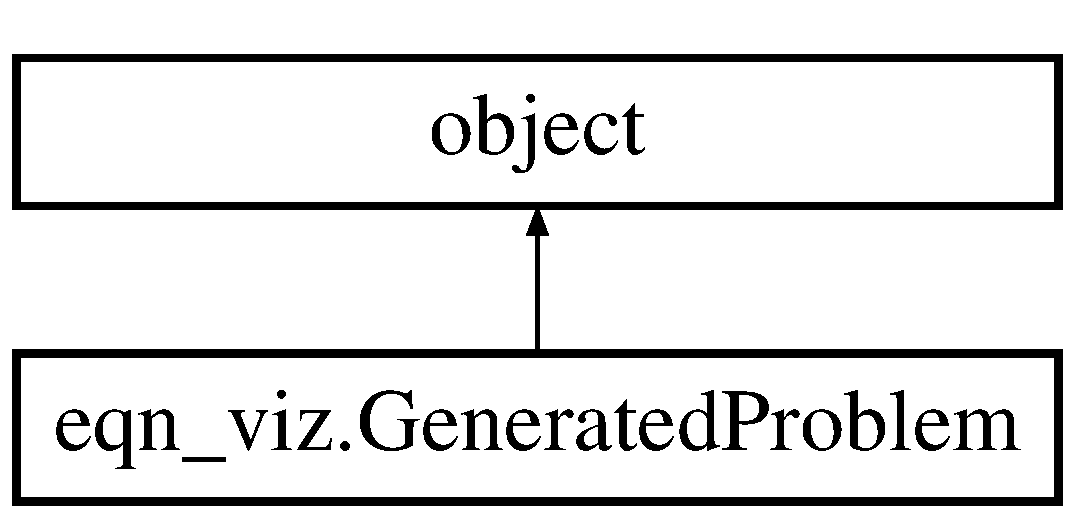
\includegraphics[height=2.000000cm]{classeqn__viz_1_1_generated_problem}
\end{center}
\end{figure}
\subsection*{Public Member Functions}
\begin{DoxyCompactItemize}
\item 
def \hyperlink{classeqn__viz_1_1_generated_problem_ad04a6f39f4f93f4a13de81de58505fb4}{\+\_\+\+\_\+init\+\_\+\+\_\+} (self, eqn\+\_\+params\+\_\+dict)
\item 
def \hyperlink{classeqn__viz_1_1_generated_problem_ae247db4ad0774a3e18f1dea1d0978c3a}{get\+Solution\+String}
\item 
def \hyperlink{classeqn__viz_1_1_generated_problem_ab7cc30e0a4a74958cb900638f3f5d844}{to\+J\+S\+O\+N\+Format} (self)
\item 
def \hyperlink{classeqn__viz_1_1_generated_problem_a2a740b018ad78a52c13acde472570669}{get\+Problem\+String} (self)
\item 
def \hyperlink{classeqn__viz_1_1_generated_problem_a5d847ddc63b6e198aac1898b90f08e02}{get\+Solution\+String\+With\+Explanations} (self)
\item 
def \hyperlink{classeqn__viz_1_1_generated_problem_a9ab6f7cd7e238344c040cda33df75a53}{get\+Selected\+Heuristics} (self)
\item 
def \hyperlink{classeqn__viz_1_1_generated_problem_a982abb22d7aff44efea7f6fac6aa903d}{get\+Applicable\+Heuristics} (self)
\end{DoxyCompactItemize}
\subsection*{Public Attributes}
\begin{DoxyCompactItemize}
\item 
\hyperlink{classeqn__viz_1_1_generated_problem_a2e0f51cffcc4ffbaba5f48e7b537e93b}{equation\+\_\+parameters}
\end{DoxyCompactItemize}


\subsection{Detailed Description}


Definition at line 95 of file eqn\+\_\+viz.\+py.



\subsection{Constructor \& Destructor Documentation}
\hypertarget{classeqn__viz_1_1_generated_problem_ad04a6f39f4f93f4a13de81de58505fb4}{}\index{eqn\+\_\+viz\+::\+Generated\+Problem@{eqn\+\_\+viz\+::\+Generated\+Problem}!\+\_\+\+\_\+init\+\_\+\+\_\+@{\+\_\+\+\_\+init\+\_\+\+\_\+}}
\index{\+\_\+\+\_\+init\+\_\+\+\_\+@{\+\_\+\+\_\+init\+\_\+\+\_\+}!eqn\+\_\+viz\+::\+Generated\+Problem@{eqn\+\_\+viz\+::\+Generated\+Problem}}
\subsubsection[{\+\_\+\+\_\+init\+\_\+\+\_\+}]{\setlength{\rightskip}{0pt plus 5cm}def eqn\+\_\+viz.\+Generated\+Problem.\+\_\+\+\_\+init\+\_\+\+\_\+ (
\begin{DoxyParamCaption}
\item[{}]{self, }
\item[{}]{eqn\+\_\+params\+\_\+dict}
\end{DoxyParamCaption}
)}\label{classeqn__viz_1_1_generated_problem_ad04a6f39f4f93f4a13de81de58505fb4}


Definition at line 96 of file eqn\+\_\+viz.\+py.



\subsection{Member Function Documentation}
\hypertarget{classeqn__viz_1_1_generated_problem_a982abb22d7aff44efea7f6fac6aa903d}{}\index{eqn\+\_\+viz\+::\+Generated\+Problem@{eqn\+\_\+viz\+::\+Generated\+Problem}!get\+Applicable\+Heuristics@{get\+Applicable\+Heuristics}}
\index{get\+Applicable\+Heuristics@{get\+Applicable\+Heuristics}!eqn\+\_\+viz\+::\+Generated\+Problem@{eqn\+\_\+viz\+::\+Generated\+Problem}}
\subsubsection[{get\+Applicable\+Heuristics}]{\setlength{\rightskip}{0pt plus 5cm}def eqn\+\_\+viz.\+Generated\+Problem.\+get\+Applicable\+Heuristics (
\begin{DoxyParamCaption}
\item[{}]{self}
\end{DoxyParamCaption}
)}\label{classeqn__viz_1_1_generated_problem_a982abb22d7aff44efea7f6fac6aa903d}


Definition at line 118 of file eqn\+\_\+viz.\+py.

\hypertarget{classeqn__viz_1_1_generated_problem_a2a740b018ad78a52c13acde472570669}{}\index{eqn\+\_\+viz\+::\+Generated\+Problem@{eqn\+\_\+viz\+::\+Generated\+Problem}!get\+Problem\+String@{get\+Problem\+String}}
\index{get\+Problem\+String@{get\+Problem\+String}!eqn\+\_\+viz\+::\+Generated\+Problem@{eqn\+\_\+viz\+::\+Generated\+Problem}}
\subsubsection[{get\+Problem\+String}]{\setlength{\rightskip}{0pt plus 5cm}def eqn\+\_\+viz.\+Generated\+Problem.\+get\+Problem\+String (
\begin{DoxyParamCaption}
\item[{}]{self}
\end{DoxyParamCaption}
)}\label{classeqn__viz_1_1_generated_problem_a2a740b018ad78a52c13acde472570669}


Definition at line 102 of file eqn\+\_\+viz.\+py.

\hypertarget{classeqn__viz_1_1_generated_problem_a9ab6f7cd7e238344c040cda33df75a53}{}\index{eqn\+\_\+viz\+::\+Generated\+Problem@{eqn\+\_\+viz\+::\+Generated\+Problem}!get\+Selected\+Heuristics@{get\+Selected\+Heuristics}}
\index{get\+Selected\+Heuristics@{get\+Selected\+Heuristics}!eqn\+\_\+viz\+::\+Generated\+Problem@{eqn\+\_\+viz\+::\+Generated\+Problem}}
\subsubsection[{get\+Selected\+Heuristics}]{\setlength{\rightskip}{0pt plus 5cm}def eqn\+\_\+viz.\+Generated\+Problem.\+get\+Selected\+Heuristics (
\begin{DoxyParamCaption}
\item[{}]{self}
\end{DoxyParamCaption}
)}\label{classeqn__viz_1_1_generated_problem_a9ab6f7cd7e238344c040cda33df75a53}


Definition at line 116 of file eqn\+\_\+viz.\+py.

\hypertarget{classeqn__viz_1_1_generated_problem_ae247db4ad0774a3e18f1dea1d0978c3a}{}\index{eqn\+\_\+viz\+::\+Generated\+Problem@{eqn\+\_\+viz\+::\+Generated\+Problem}!get\+Solution\+String@{get\+Solution\+String}}
\index{get\+Solution\+String@{get\+Solution\+String}!eqn\+\_\+viz\+::\+Generated\+Problem@{eqn\+\_\+viz\+::\+Generated\+Problem}}
\subsubsection[{get\+Solution\+String}]{\setlength{\rightskip}{0pt plus 5cm}def eqn\+\_\+viz.\+Generated\+Problem.\+get\+Solution\+String (
\begin{DoxyParamCaption}
\item[{}]{self, }
\item[{}]{as\+\_\+latex = {\ttfamily False}, }
\item[{}]{json\+\_\+output = {\ttfamily False}}
\end{DoxyParamCaption}
)}\label{classeqn__viz_1_1_generated_problem_ae247db4ad0774a3e18f1dea1d0978c3a}


Definition at line 98 of file eqn\+\_\+viz.\+py.

\hypertarget{classeqn__viz_1_1_generated_problem_a5d847ddc63b6e198aac1898b90f08e02}{}\index{eqn\+\_\+viz\+::\+Generated\+Problem@{eqn\+\_\+viz\+::\+Generated\+Problem}!get\+Solution\+String\+With\+Explanations@{get\+Solution\+String\+With\+Explanations}}
\index{get\+Solution\+String\+With\+Explanations@{get\+Solution\+String\+With\+Explanations}!eqn\+\_\+viz\+::\+Generated\+Problem@{eqn\+\_\+viz\+::\+Generated\+Problem}}
\subsubsection[{get\+Solution\+String\+With\+Explanations}]{\setlength{\rightskip}{0pt plus 5cm}def eqn\+\_\+viz.\+Generated\+Problem.\+get\+Solution\+String\+With\+Explanations (
\begin{DoxyParamCaption}
\item[{}]{self}
\end{DoxyParamCaption}
)}\label{classeqn__viz_1_1_generated_problem_a5d847ddc63b6e198aac1898b90f08e02}


Definition at line 105 of file eqn\+\_\+viz.\+py.

\hypertarget{classeqn__viz_1_1_generated_problem_ab7cc30e0a4a74958cb900638f3f5d844}{}\index{eqn\+\_\+viz\+::\+Generated\+Problem@{eqn\+\_\+viz\+::\+Generated\+Problem}!to\+J\+S\+O\+N\+Format@{to\+J\+S\+O\+N\+Format}}
\index{to\+J\+S\+O\+N\+Format@{to\+J\+S\+O\+N\+Format}!eqn\+\_\+viz\+::\+Generated\+Problem@{eqn\+\_\+viz\+::\+Generated\+Problem}}
\subsubsection[{to\+J\+S\+O\+N\+Format}]{\setlength{\rightskip}{0pt plus 5cm}def eqn\+\_\+viz.\+Generated\+Problem.\+to\+J\+S\+O\+N\+Format (
\begin{DoxyParamCaption}
\item[{}]{self}
\end{DoxyParamCaption}
)}\label{classeqn__viz_1_1_generated_problem_ab7cc30e0a4a74958cb900638f3f5d844}


Definition at line 100 of file eqn\+\_\+viz.\+py.



\subsection{Member Data Documentation}
\hypertarget{classeqn__viz_1_1_generated_problem_a2e0f51cffcc4ffbaba5f48e7b537e93b}{}\index{eqn\+\_\+viz\+::\+Generated\+Problem@{eqn\+\_\+viz\+::\+Generated\+Problem}!equation\+\_\+parameters@{equation\+\_\+parameters}}
\index{equation\+\_\+parameters@{equation\+\_\+parameters}!eqn\+\_\+viz\+::\+Generated\+Problem@{eqn\+\_\+viz\+::\+Generated\+Problem}}
\subsubsection[{equation\+\_\+parameters}]{\setlength{\rightskip}{0pt plus 5cm}eqn\+\_\+viz.\+Generated\+Problem.\+equation\+\_\+parameters}\label{classeqn__viz_1_1_generated_problem_a2e0f51cffcc4ffbaba5f48e7b537e93b}


Definition at line 97 of file eqn\+\_\+viz.\+py.



The documentation for this class was generated from the following file\+:\begin{DoxyCompactItemize}
\item 
\hyperlink{eqn__viz_8py}{eqn\+\_\+viz.\+py}\end{DoxyCompactItemize}

\hypertarget{class_prolog_rules_parser_1_1_prolog_rules_parser_1_1_guessrule_context}{}\section{Prolog\+Rules\+Parser.\+Prolog\+Rules\+Parser.\+Guessrule\+Context Class Reference}
\label{class_prolog_rules_parser_1_1_prolog_rules_parser_1_1_guessrule_context}\index{Prolog\+Rules\+Parser.\+Prolog\+Rules\+Parser.\+Guessrule\+Context@{Prolog\+Rules\+Parser.\+Prolog\+Rules\+Parser.\+Guessrule\+Context}}
Inheritance diagram for Prolog\+Rules\+Parser.\+Prolog\+Rules\+Parser.\+Guessrule\+Context\+:\begin{figure}[H]
\begin{center}
\leavevmode
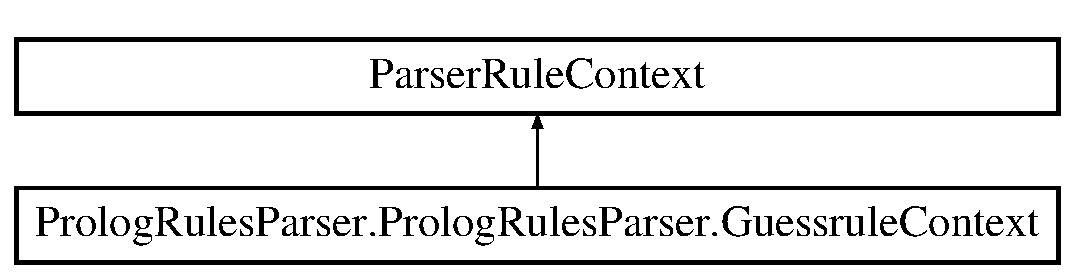
\includegraphics[height=2.000000cm]{class_prolog_rules_parser_1_1_prolog_rules_parser_1_1_guessrule_context}
\end{center}
\end{figure}
\subsection*{Public Member Functions}
\begin{DoxyCompactItemize}
\item 
def \hyperlink{class_prolog_rules_parser_1_1_prolog_rules_parser_1_1_guessrule_context_ae1a548898a05a40db4e5e00dfc194c20}{\+\_\+\+\_\+init\+\_\+\+\_\+}
\item 
def \hyperlink{class_prolog_rules_parser_1_1_prolog_rules_parser_1_1_guessrule_context_a2348ed6102b18d1f34e905c302c38bd2}{predicate} (self)
\item 
def \hyperlink{class_prolog_rules_parser_1_1_prolog_rules_parser_1_1_guessrule_context_ab4c841a5e28076ef1bc7ed425f82271b}{N\+U\+M\+B\+E\+R}
\item 
def \hyperlink{class_prolog_rules_parser_1_1_prolog_rules_parser_1_1_guessrule_context_ae688607e95c8a038062b890164d01203}{rulebody}
\item 
def \hyperlink{class_prolog_rules_parser_1_1_prolog_rules_parser_1_1_guessrule_context_a5df7b953cfd85b7aa06564bfd92dd0be}{get\+Rule\+Index} (self)
\item 
def \hyperlink{class_prolog_rules_parser_1_1_prolog_rules_parser_1_1_guessrule_context_af3fa7ee052296e884170cca95ed8fa34}{enter\+Rule} (self, listener)
\item 
def \hyperlink{class_prolog_rules_parser_1_1_prolog_rules_parser_1_1_guessrule_context_aea1f6d1f13e01a7eb2c5c0203e2fd555}{exit\+Rule} (self, listener)
\end{DoxyCompactItemize}
\subsection*{Public Attributes}
\begin{DoxyCompactItemize}
\item 
\hyperlink{class_prolog_rules_parser_1_1_prolog_rules_parser_1_1_guessrule_context_abc024afc97dd2b002b79c0f2b5aaa641}{parser}
\end{DoxyCompactItemize}


\subsection{Detailed Description}


Definition at line 447 of file Prolog\+Rules\+Parser.\+py.



\subsection{Constructor \& Destructor Documentation}
\hypertarget{class_prolog_rules_parser_1_1_prolog_rules_parser_1_1_guessrule_context_ae1a548898a05a40db4e5e00dfc194c20}{}\index{Prolog\+Rules\+Parser\+::\+Prolog\+Rules\+Parser\+::\+Guessrule\+Context@{Prolog\+Rules\+Parser\+::\+Prolog\+Rules\+Parser\+::\+Guessrule\+Context}!\+\_\+\+\_\+init\+\_\+\+\_\+@{\+\_\+\+\_\+init\+\_\+\+\_\+}}
\index{\+\_\+\+\_\+init\+\_\+\+\_\+@{\+\_\+\+\_\+init\+\_\+\+\_\+}!Prolog\+Rules\+Parser\+::\+Prolog\+Rules\+Parser\+::\+Guessrule\+Context@{Prolog\+Rules\+Parser\+::\+Prolog\+Rules\+Parser\+::\+Guessrule\+Context}}
\subsubsection[{\+\_\+\+\_\+init\+\_\+\+\_\+}]{\setlength{\rightskip}{0pt plus 5cm}def Prolog\+Rules\+Parser.\+Prolog\+Rules\+Parser.\+Guessrule\+Context.\+\_\+\+\_\+init\+\_\+\+\_\+ (
\begin{DoxyParamCaption}
\item[{}]{self, }
\item[{}]{parser, }
\item[{}]{parent = {\ttfamily None}, }
\item[{}]{invoking\+State = {\ttfamily -\/1}}
\end{DoxyParamCaption}
)}\label{class_prolog_rules_parser_1_1_prolog_rules_parser_1_1_guessrule_context_ae1a548898a05a40db4e5e00dfc194c20}


Definition at line 449 of file Prolog\+Rules\+Parser.\+py.



\subsection{Member Function Documentation}
\hypertarget{class_prolog_rules_parser_1_1_prolog_rules_parser_1_1_guessrule_context_af3fa7ee052296e884170cca95ed8fa34}{}\index{Prolog\+Rules\+Parser\+::\+Prolog\+Rules\+Parser\+::\+Guessrule\+Context@{Prolog\+Rules\+Parser\+::\+Prolog\+Rules\+Parser\+::\+Guessrule\+Context}!enter\+Rule@{enter\+Rule}}
\index{enter\+Rule@{enter\+Rule}!Prolog\+Rules\+Parser\+::\+Prolog\+Rules\+Parser\+::\+Guessrule\+Context@{Prolog\+Rules\+Parser\+::\+Prolog\+Rules\+Parser\+::\+Guessrule\+Context}}
\subsubsection[{enter\+Rule}]{\setlength{\rightskip}{0pt plus 5cm}def Prolog\+Rules\+Parser.\+Prolog\+Rules\+Parser.\+Guessrule\+Context.\+enter\+Rule (
\begin{DoxyParamCaption}
\item[{}]{self, }
\item[{}]{listener}
\end{DoxyParamCaption}
)}\label{class_prolog_rules_parser_1_1_prolog_rules_parser_1_1_guessrule_context_af3fa7ee052296e884170cca95ed8fa34}


Definition at line 473 of file Prolog\+Rules\+Parser.\+py.

\hypertarget{class_prolog_rules_parser_1_1_prolog_rules_parser_1_1_guessrule_context_aea1f6d1f13e01a7eb2c5c0203e2fd555}{}\index{Prolog\+Rules\+Parser\+::\+Prolog\+Rules\+Parser\+::\+Guessrule\+Context@{Prolog\+Rules\+Parser\+::\+Prolog\+Rules\+Parser\+::\+Guessrule\+Context}!exit\+Rule@{exit\+Rule}}
\index{exit\+Rule@{exit\+Rule}!Prolog\+Rules\+Parser\+::\+Prolog\+Rules\+Parser\+::\+Guessrule\+Context@{Prolog\+Rules\+Parser\+::\+Prolog\+Rules\+Parser\+::\+Guessrule\+Context}}
\subsubsection[{exit\+Rule}]{\setlength{\rightskip}{0pt plus 5cm}def Prolog\+Rules\+Parser.\+Prolog\+Rules\+Parser.\+Guessrule\+Context.\+exit\+Rule (
\begin{DoxyParamCaption}
\item[{}]{self, }
\item[{}]{listener}
\end{DoxyParamCaption}
)}\label{class_prolog_rules_parser_1_1_prolog_rules_parser_1_1_guessrule_context_aea1f6d1f13e01a7eb2c5c0203e2fd555}


Definition at line 477 of file Prolog\+Rules\+Parser.\+py.

\hypertarget{class_prolog_rules_parser_1_1_prolog_rules_parser_1_1_guessrule_context_a5df7b953cfd85b7aa06564bfd92dd0be}{}\index{Prolog\+Rules\+Parser\+::\+Prolog\+Rules\+Parser\+::\+Guessrule\+Context@{Prolog\+Rules\+Parser\+::\+Prolog\+Rules\+Parser\+::\+Guessrule\+Context}!get\+Rule\+Index@{get\+Rule\+Index}}
\index{get\+Rule\+Index@{get\+Rule\+Index}!Prolog\+Rules\+Parser\+::\+Prolog\+Rules\+Parser\+::\+Guessrule\+Context@{Prolog\+Rules\+Parser\+::\+Prolog\+Rules\+Parser\+::\+Guessrule\+Context}}
\subsubsection[{get\+Rule\+Index}]{\setlength{\rightskip}{0pt plus 5cm}def Prolog\+Rules\+Parser.\+Prolog\+Rules\+Parser.\+Guessrule\+Context.\+get\+Rule\+Index (
\begin{DoxyParamCaption}
\item[{}]{self}
\end{DoxyParamCaption}
)}\label{class_prolog_rules_parser_1_1_prolog_rules_parser_1_1_guessrule_context_a5df7b953cfd85b7aa06564bfd92dd0be}


Definition at line 470 of file Prolog\+Rules\+Parser.\+py.

\hypertarget{class_prolog_rules_parser_1_1_prolog_rules_parser_1_1_guessrule_context_ab4c841a5e28076ef1bc7ed425f82271b}{}\index{Prolog\+Rules\+Parser\+::\+Prolog\+Rules\+Parser\+::\+Guessrule\+Context@{Prolog\+Rules\+Parser\+::\+Prolog\+Rules\+Parser\+::\+Guessrule\+Context}!N\+U\+M\+B\+E\+R@{N\+U\+M\+B\+E\+R}}
\index{N\+U\+M\+B\+E\+R@{N\+U\+M\+B\+E\+R}!Prolog\+Rules\+Parser\+::\+Prolog\+Rules\+Parser\+::\+Guessrule\+Context@{Prolog\+Rules\+Parser\+::\+Prolog\+Rules\+Parser\+::\+Guessrule\+Context}}
\subsubsection[{N\+U\+M\+B\+E\+R}]{\setlength{\rightskip}{0pt plus 5cm}def Prolog\+Rules\+Parser.\+Prolog\+Rules\+Parser.\+Guessrule\+Context.\+N\+U\+M\+B\+E\+R (
\begin{DoxyParamCaption}
\item[{}]{self, }
\item[{}]{i = {\ttfamily None}}
\end{DoxyParamCaption}
)}\label{class_prolog_rules_parser_1_1_prolog_rules_parser_1_1_guessrule_context_ab4c841a5e28076ef1bc7ed425f82271b}


Definition at line 457 of file Prolog\+Rules\+Parser.\+py.

\hypertarget{class_prolog_rules_parser_1_1_prolog_rules_parser_1_1_guessrule_context_a2348ed6102b18d1f34e905c302c38bd2}{}\index{Prolog\+Rules\+Parser\+::\+Prolog\+Rules\+Parser\+::\+Guessrule\+Context@{Prolog\+Rules\+Parser\+::\+Prolog\+Rules\+Parser\+::\+Guessrule\+Context}!predicate@{predicate}}
\index{predicate@{predicate}!Prolog\+Rules\+Parser\+::\+Prolog\+Rules\+Parser\+::\+Guessrule\+Context@{Prolog\+Rules\+Parser\+::\+Prolog\+Rules\+Parser\+::\+Guessrule\+Context}}
\subsubsection[{predicate}]{\setlength{\rightskip}{0pt plus 5cm}def Prolog\+Rules\+Parser.\+Prolog\+Rules\+Parser.\+Guessrule\+Context.\+predicate (
\begin{DoxyParamCaption}
\item[{}]{self}
\end{DoxyParamCaption}
)}\label{class_prolog_rules_parser_1_1_prolog_rules_parser_1_1_guessrule_context_a2348ed6102b18d1f34e905c302c38bd2}


Definition at line 453 of file Prolog\+Rules\+Parser.\+py.

\hypertarget{class_prolog_rules_parser_1_1_prolog_rules_parser_1_1_guessrule_context_ae688607e95c8a038062b890164d01203}{}\index{Prolog\+Rules\+Parser\+::\+Prolog\+Rules\+Parser\+::\+Guessrule\+Context@{Prolog\+Rules\+Parser\+::\+Prolog\+Rules\+Parser\+::\+Guessrule\+Context}!rulebody@{rulebody}}
\index{rulebody@{rulebody}!Prolog\+Rules\+Parser\+::\+Prolog\+Rules\+Parser\+::\+Guessrule\+Context@{Prolog\+Rules\+Parser\+::\+Prolog\+Rules\+Parser\+::\+Guessrule\+Context}}
\subsubsection[{rulebody}]{\setlength{\rightskip}{0pt plus 5cm}def Prolog\+Rules\+Parser.\+Prolog\+Rules\+Parser.\+Guessrule\+Context.\+rulebody (
\begin{DoxyParamCaption}
\item[{}]{self, }
\item[{}]{i = {\ttfamily None}}
\end{DoxyParamCaption}
)}\label{class_prolog_rules_parser_1_1_prolog_rules_parser_1_1_guessrule_context_ae688607e95c8a038062b890164d01203}


Definition at line 463 of file Prolog\+Rules\+Parser.\+py.



\subsection{Member Data Documentation}
\hypertarget{class_prolog_rules_parser_1_1_prolog_rules_parser_1_1_guessrule_context_abc024afc97dd2b002b79c0f2b5aaa641}{}\index{Prolog\+Rules\+Parser\+::\+Prolog\+Rules\+Parser\+::\+Guessrule\+Context@{Prolog\+Rules\+Parser\+::\+Prolog\+Rules\+Parser\+::\+Guessrule\+Context}!parser@{parser}}
\index{parser@{parser}!Prolog\+Rules\+Parser\+::\+Prolog\+Rules\+Parser\+::\+Guessrule\+Context@{Prolog\+Rules\+Parser\+::\+Prolog\+Rules\+Parser\+::\+Guessrule\+Context}}
\subsubsection[{parser}]{\setlength{\rightskip}{0pt plus 5cm}Prolog\+Rules\+Parser.\+Prolog\+Rules\+Parser.\+Guessrule\+Context.\+parser}\label{class_prolog_rules_parser_1_1_prolog_rules_parser_1_1_guessrule_context_abc024afc97dd2b002b79c0f2b5aaa641}


Definition at line 451 of file Prolog\+Rules\+Parser.\+py.



The documentation for this class was generated from the following file\+:\begin{DoxyCompactItemize}
\item 
\hyperlink{_prolog_rules_parser_8py}{Prolog\+Rules\+Parser.\+py}\end{DoxyCompactItemize}

\hypertarget{class_prolog_rules_parser_1_1_prolog_rules_parser_1_1_identifier_context}{}\section{Prolog\+Rules\+Parser.\+Prolog\+Rules\+Parser.\+Identifier\+Context Class Reference}
\label{class_prolog_rules_parser_1_1_prolog_rules_parser_1_1_identifier_context}\index{Prolog\+Rules\+Parser.\+Prolog\+Rules\+Parser.\+Identifier\+Context@{Prolog\+Rules\+Parser.\+Prolog\+Rules\+Parser.\+Identifier\+Context}}
Inheritance diagram for Prolog\+Rules\+Parser.\+Prolog\+Rules\+Parser.\+Identifier\+Context\+:\begin{figure}[H]
\begin{center}
\leavevmode
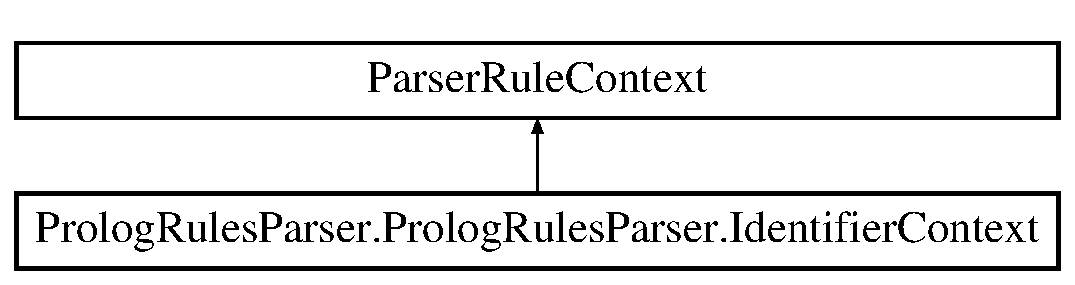
\includegraphics[height=2.000000cm]{class_prolog_rules_parser_1_1_prolog_rules_parser_1_1_identifier_context}
\end{center}
\end{figure}
\subsection*{Public Member Functions}
\begin{DoxyCompactItemize}
\item 
def \hyperlink{class_prolog_rules_parser_1_1_prolog_rules_parser_1_1_identifier_context_a4e27087e457b0a1a30e267296c0b5d27}{\+\_\+\+\_\+init\+\_\+\+\_\+}
\item 
def \hyperlink{class_prolog_rules_parser_1_1_prolog_rules_parser_1_1_identifier_context_ae0051cb257cc23bb7ba7395229267e54}{W\+O\+R\+D} (self)
\item 
def \hyperlink{class_prolog_rules_parser_1_1_prolog_rules_parser_1_1_identifier_context_a0c78b930d7b0f086af8898f27446003f}{get\+Rule\+Index} (self)
\item 
def \hyperlink{class_prolog_rules_parser_1_1_prolog_rules_parser_1_1_identifier_context_a13773579c93b133bd3d76ae74fb48da4}{enter\+Rule} (self, listener)
\item 
def \hyperlink{class_prolog_rules_parser_1_1_prolog_rules_parser_1_1_identifier_context_a31f5b17b8fb5e23d9c73fa8428babc85}{exit\+Rule} (self, listener)
\end{DoxyCompactItemize}
\subsection*{Public Attributes}
\begin{DoxyCompactItemize}
\item 
\hyperlink{class_prolog_rules_parser_1_1_prolog_rules_parser_1_1_identifier_context_abbd5df64720a0e1958526c13e82fd390}{parser}
\end{DoxyCompactItemize}


\subsection{Detailed Description}


Definition at line 1152 of file Prolog\+Rules\+Parser.\+py.



\subsection{Constructor \& Destructor Documentation}
\hypertarget{class_prolog_rules_parser_1_1_prolog_rules_parser_1_1_identifier_context_a4e27087e457b0a1a30e267296c0b5d27}{}\index{Prolog\+Rules\+Parser\+::\+Prolog\+Rules\+Parser\+::\+Identifier\+Context@{Prolog\+Rules\+Parser\+::\+Prolog\+Rules\+Parser\+::\+Identifier\+Context}!\+\_\+\+\_\+init\+\_\+\+\_\+@{\+\_\+\+\_\+init\+\_\+\+\_\+}}
\index{\+\_\+\+\_\+init\+\_\+\+\_\+@{\+\_\+\+\_\+init\+\_\+\+\_\+}!Prolog\+Rules\+Parser\+::\+Prolog\+Rules\+Parser\+::\+Identifier\+Context@{Prolog\+Rules\+Parser\+::\+Prolog\+Rules\+Parser\+::\+Identifier\+Context}}
\subsubsection[{\+\_\+\+\_\+init\+\_\+\+\_\+}]{\setlength{\rightskip}{0pt plus 5cm}def Prolog\+Rules\+Parser.\+Prolog\+Rules\+Parser.\+Identifier\+Context.\+\_\+\+\_\+init\+\_\+\+\_\+ (
\begin{DoxyParamCaption}
\item[{}]{self, }
\item[{}]{parser, }
\item[{}]{parent = {\ttfamily None}, }
\item[{}]{invoking\+State = {\ttfamily -\/1}}
\end{DoxyParamCaption}
)}\label{class_prolog_rules_parser_1_1_prolog_rules_parser_1_1_identifier_context_a4e27087e457b0a1a30e267296c0b5d27}


Definition at line 1154 of file Prolog\+Rules\+Parser.\+py.



\subsection{Member Function Documentation}
\hypertarget{class_prolog_rules_parser_1_1_prolog_rules_parser_1_1_identifier_context_a13773579c93b133bd3d76ae74fb48da4}{}\index{Prolog\+Rules\+Parser\+::\+Prolog\+Rules\+Parser\+::\+Identifier\+Context@{Prolog\+Rules\+Parser\+::\+Prolog\+Rules\+Parser\+::\+Identifier\+Context}!enter\+Rule@{enter\+Rule}}
\index{enter\+Rule@{enter\+Rule}!Prolog\+Rules\+Parser\+::\+Prolog\+Rules\+Parser\+::\+Identifier\+Context@{Prolog\+Rules\+Parser\+::\+Prolog\+Rules\+Parser\+::\+Identifier\+Context}}
\subsubsection[{enter\+Rule}]{\setlength{\rightskip}{0pt plus 5cm}def Prolog\+Rules\+Parser.\+Prolog\+Rules\+Parser.\+Identifier\+Context.\+enter\+Rule (
\begin{DoxyParamCaption}
\item[{}]{self, }
\item[{}]{listener}
\end{DoxyParamCaption}
)}\label{class_prolog_rules_parser_1_1_prolog_rules_parser_1_1_identifier_context_a13773579c93b133bd3d76ae74fb48da4}


Definition at line 1164 of file Prolog\+Rules\+Parser.\+py.

\hypertarget{class_prolog_rules_parser_1_1_prolog_rules_parser_1_1_identifier_context_a31f5b17b8fb5e23d9c73fa8428babc85}{}\index{Prolog\+Rules\+Parser\+::\+Prolog\+Rules\+Parser\+::\+Identifier\+Context@{Prolog\+Rules\+Parser\+::\+Prolog\+Rules\+Parser\+::\+Identifier\+Context}!exit\+Rule@{exit\+Rule}}
\index{exit\+Rule@{exit\+Rule}!Prolog\+Rules\+Parser\+::\+Prolog\+Rules\+Parser\+::\+Identifier\+Context@{Prolog\+Rules\+Parser\+::\+Prolog\+Rules\+Parser\+::\+Identifier\+Context}}
\subsubsection[{exit\+Rule}]{\setlength{\rightskip}{0pt plus 5cm}def Prolog\+Rules\+Parser.\+Prolog\+Rules\+Parser.\+Identifier\+Context.\+exit\+Rule (
\begin{DoxyParamCaption}
\item[{}]{self, }
\item[{}]{listener}
\end{DoxyParamCaption}
)}\label{class_prolog_rules_parser_1_1_prolog_rules_parser_1_1_identifier_context_a31f5b17b8fb5e23d9c73fa8428babc85}


Definition at line 1168 of file Prolog\+Rules\+Parser.\+py.

\hypertarget{class_prolog_rules_parser_1_1_prolog_rules_parser_1_1_identifier_context_a0c78b930d7b0f086af8898f27446003f}{}\index{Prolog\+Rules\+Parser\+::\+Prolog\+Rules\+Parser\+::\+Identifier\+Context@{Prolog\+Rules\+Parser\+::\+Prolog\+Rules\+Parser\+::\+Identifier\+Context}!get\+Rule\+Index@{get\+Rule\+Index}}
\index{get\+Rule\+Index@{get\+Rule\+Index}!Prolog\+Rules\+Parser\+::\+Prolog\+Rules\+Parser\+::\+Identifier\+Context@{Prolog\+Rules\+Parser\+::\+Prolog\+Rules\+Parser\+::\+Identifier\+Context}}
\subsubsection[{get\+Rule\+Index}]{\setlength{\rightskip}{0pt plus 5cm}def Prolog\+Rules\+Parser.\+Prolog\+Rules\+Parser.\+Identifier\+Context.\+get\+Rule\+Index (
\begin{DoxyParamCaption}
\item[{}]{self}
\end{DoxyParamCaption}
)}\label{class_prolog_rules_parser_1_1_prolog_rules_parser_1_1_identifier_context_a0c78b930d7b0f086af8898f27446003f}


Definition at line 1161 of file Prolog\+Rules\+Parser.\+py.

\hypertarget{class_prolog_rules_parser_1_1_prolog_rules_parser_1_1_identifier_context_ae0051cb257cc23bb7ba7395229267e54}{}\index{Prolog\+Rules\+Parser\+::\+Prolog\+Rules\+Parser\+::\+Identifier\+Context@{Prolog\+Rules\+Parser\+::\+Prolog\+Rules\+Parser\+::\+Identifier\+Context}!W\+O\+R\+D@{W\+O\+R\+D}}
\index{W\+O\+R\+D@{W\+O\+R\+D}!Prolog\+Rules\+Parser\+::\+Prolog\+Rules\+Parser\+::\+Identifier\+Context@{Prolog\+Rules\+Parser\+::\+Prolog\+Rules\+Parser\+::\+Identifier\+Context}}
\subsubsection[{W\+O\+R\+D}]{\setlength{\rightskip}{0pt plus 5cm}def Prolog\+Rules\+Parser.\+Prolog\+Rules\+Parser.\+Identifier\+Context.\+W\+O\+R\+D (
\begin{DoxyParamCaption}
\item[{}]{self}
\end{DoxyParamCaption}
)}\label{class_prolog_rules_parser_1_1_prolog_rules_parser_1_1_identifier_context_ae0051cb257cc23bb7ba7395229267e54}


Definition at line 1158 of file Prolog\+Rules\+Parser.\+py.



\subsection{Member Data Documentation}
\hypertarget{class_prolog_rules_parser_1_1_prolog_rules_parser_1_1_identifier_context_abbd5df64720a0e1958526c13e82fd390}{}\index{Prolog\+Rules\+Parser\+::\+Prolog\+Rules\+Parser\+::\+Identifier\+Context@{Prolog\+Rules\+Parser\+::\+Prolog\+Rules\+Parser\+::\+Identifier\+Context}!parser@{parser}}
\index{parser@{parser}!Prolog\+Rules\+Parser\+::\+Prolog\+Rules\+Parser\+::\+Identifier\+Context@{Prolog\+Rules\+Parser\+::\+Prolog\+Rules\+Parser\+::\+Identifier\+Context}}
\subsubsection[{parser}]{\setlength{\rightskip}{0pt plus 5cm}Prolog\+Rules\+Parser.\+Prolog\+Rules\+Parser.\+Identifier\+Context.\+parser}\label{class_prolog_rules_parser_1_1_prolog_rules_parser_1_1_identifier_context_abbd5df64720a0e1958526c13e82fd390}


Definition at line 1156 of file Prolog\+Rules\+Parser.\+py.



The documentation for this class was generated from the following file\+:\begin{DoxyCompactItemize}
\item 
\hyperlink{_prolog_rules_parser_8py}{Prolog\+Rules\+Parser.\+py}\end{DoxyCompactItemize}

\hypertarget{class_prolog_rules_parser_1_1_prolog_rules_parser_1_1_mathexpr_context}{}\section{Prolog\+Rules\+Parser.\+Prolog\+Rules\+Parser.\+Mathexpr\+Context Class Reference}
\label{class_prolog_rules_parser_1_1_prolog_rules_parser_1_1_mathexpr_context}\index{Prolog\+Rules\+Parser.\+Prolog\+Rules\+Parser.\+Mathexpr\+Context@{Prolog\+Rules\+Parser.\+Prolog\+Rules\+Parser.\+Mathexpr\+Context}}
Inheritance diagram for Prolog\+Rules\+Parser.\+Prolog\+Rules\+Parser.\+Mathexpr\+Context\+:\begin{figure}[H]
\begin{center}
\leavevmode
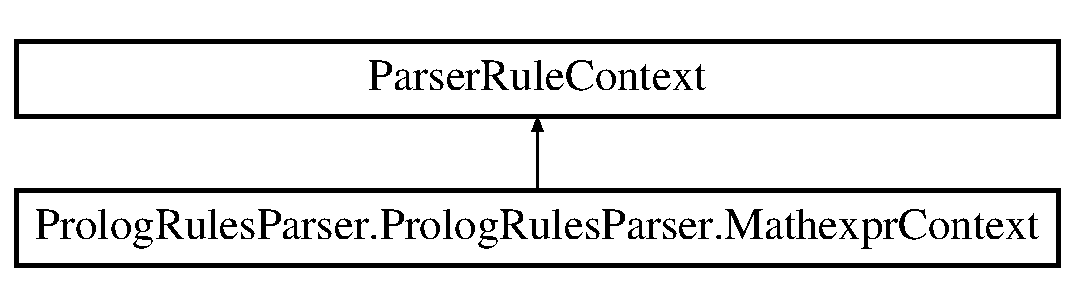
\includegraphics[height=2.000000cm]{class_prolog_rules_parser_1_1_prolog_rules_parser_1_1_mathexpr_context}
\end{center}
\end{figure}
\subsection*{Public Member Functions}
\begin{DoxyCompactItemize}
\item 
def \hyperlink{class_prolog_rules_parser_1_1_prolog_rules_parser_1_1_mathexpr_context_ac65feb745a3d272c76c7b02744499965}{\+\_\+\+\_\+init\+\_\+\+\_\+}
\item 
def \hyperlink{class_prolog_rules_parser_1_1_prolog_rules_parser_1_1_mathexpr_context_a58091aa625a7633b64a3b75ea41051d2}{mathexpr} (self)
\item 
def \hyperlink{class_prolog_rules_parser_1_1_prolog_rules_parser_1_1_mathexpr_context_a739b415e126861043fd4b0cb7fdbeda9}{predicate} (self)
\item 
def \hyperlink{class_prolog_rules_parser_1_1_prolog_rules_parser_1_1_mathexpr_context_a7c11e2387b7216f3d93597d044f9fcba}{atom} (self)
\item 
def \hyperlink{class_prolog_rules_parser_1_1_prolog_rules_parser_1_1_mathexpr_context_a24b387aace761d5189e3fe80e3ef7653}{O\+P\+E\+R\+A\+T\+O\+R} (self)
\item 
def \hyperlink{class_prolog_rules_parser_1_1_prolog_rules_parser_1_1_mathexpr_context_a49b6d329e8fead29bb8e4deda9ace614}{get\+Rule\+Index} (self)
\item 
def \hyperlink{class_prolog_rules_parser_1_1_prolog_rules_parser_1_1_mathexpr_context_a305bcd3766e155aa9fecea8b4bce2005}{enter\+Rule} (self, listener)
\item 
def \hyperlink{class_prolog_rules_parser_1_1_prolog_rules_parser_1_1_mathexpr_context_ab0be52a445a692e94faac0704928053b}{exit\+Rule} (self, listener)
\end{DoxyCompactItemize}
\subsection*{Public Attributes}
\begin{DoxyCompactItemize}
\item 
\hyperlink{class_prolog_rules_parser_1_1_prolog_rules_parser_1_1_mathexpr_context_ac8dc4d30ca3371198e7bb5db972832b8}{parser}
\end{DoxyCompactItemize}


\subsection{Detailed Description}


Definition at line 904 of file Prolog\+Rules\+Parser.\+py.



\subsection{Constructor \& Destructor Documentation}
\hypertarget{class_prolog_rules_parser_1_1_prolog_rules_parser_1_1_mathexpr_context_ac65feb745a3d272c76c7b02744499965}{}\index{Prolog\+Rules\+Parser\+::\+Prolog\+Rules\+Parser\+::\+Mathexpr\+Context@{Prolog\+Rules\+Parser\+::\+Prolog\+Rules\+Parser\+::\+Mathexpr\+Context}!\+\_\+\+\_\+init\+\_\+\+\_\+@{\+\_\+\+\_\+init\+\_\+\+\_\+}}
\index{\+\_\+\+\_\+init\+\_\+\+\_\+@{\+\_\+\+\_\+init\+\_\+\+\_\+}!Prolog\+Rules\+Parser\+::\+Prolog\+Rules\+Parser\+::\+Mathexpr\+Context@{Prolog\+Rules\+Parser\+::\+Prolog\+Rules\+Parser\+::\+Mathexpr\+Context}}
\subsubsection[{\+\_\+\+\_\+init\+\_\+\+\_\+}]{\setlength{\rightskip}{0pt plus 5cm}def Prolog\+Rules\+Parser.\+Prolog\+Rules\+Parser.\+Mathexpr\+Context.\+\_\+\+\_\+init\+\_\+\+\_\+ (
\begin{DoxyParamCaption}
\item[{}]{self, }
\item[{}]{parser, }
\item[{}]{parent = {\ttfamily None}, }
\item[{}]{invoking\+State = {\ttfamily -\/1}}
\end{DoxyParamCaption}
)}\label{class_prolog_rules_parser_1_1_prolog_rules_parser_1_1_mathexpr_context_ac65feb745a3d272c76c7b02744499965}


Definition at line 906 of file Prolog\+Rules\+Parser.\+py.



\subsection{Member Function Documentation}
\hypertarget{class_prolog_rules_parser_1_1_prolog_rules_parser_1_1_mathexpr_context_a7c11e2387b7216f3d93597d044f9fcba}{}\index{Prolog\+Rules\+Parser\+::\+Prolog\+Rules\+Parser\+::\+Mathexpr\+Context@{Prolog\+Rules\+Parser\+::\+Prolog\+Rules\+Parser\+::\+Mathexpr\+Context}!atom@{atom}}
\index{atom@{atom}!Prolog\+Rules\+Parser\+::\+Prolog\+Rules\+Parser\+::\+Mathexpr\+Context@{Prolog\+Rules\+Parser\+::\+Prolog\+Rules\+Parser\+::\+Mathexpr\+Context}}
\subsubsection[{atom}]{\setlength{\rightskip}{0pt plus 5cm}def Prolog\+Rules\+Parser.\+Prolog\+Rules\+Parser.\+Mathexpr\+Context.\+atom (
\begin{DoxyParamCaption}
\item[{}]{self}
\end{DoxyParamCaption}
)}\label{class_prolog_rules_parser_1_1_prolog_rules_parser_1_1_mathexpr_context_a7c11e2387b7216f3d93597d044f9fcba}


Definition at line 918 of file Prolog\+Rules\+Parser.\+py.

\hypertarget{class_prolog_rules_parser_1_1_prolog_rules_parser_1_1_mathexpr_context_a305bcd3766e155aa9fecea8b4bce2005}{}\index{Prolog\+Rules\+Parser\+::\+Prolog\+Rules\+Parser\+::\+Mathexpr\+Context@{Prolog\+Rules\+Parser\+::\+Prolog\+Rules\+Parser\+::\+Mathexpr\+Context}!enter\+Rule@{enter\+Rule}}
\index{enter\+Rule@{enter\+Rule}!Prolog\+Rules\+Parser\+::\+Prolog\+Rules\+Parser\+::\+Mathexpr\+Context@{Prolog\+Rules\+Parser\+::\+Prolog\+Rules\+Parser\+::\+Mathexpr\+Context}}
\subsubsection[{enter\+Rule}]{\setlength{\rightskip}{0pt plus 5cm}def Prolog\+Rules\+Parser.\+Prolog\+Rules\+Parser.\+Mathexpr\+Context.\+enter\+Rule (
\begin{DoxyParamCaption}
\item[{}]{self, }
\item[{}]{listener}
\end{DoxyParamCaption}
)}\label{class_prolog_rules_parser_1_1_prolog_rules_parser_1_1_mathexpr_context_a305bcd3766e155aa9fecea8b4bce2005}


Definition at line 928 of file Prolog\+Rules\+Parser.\+py.

\hypertarget{class_prolog_rules_parser_1_1_prolog_rules_parser_1_1_mathexpr_context_ab0be52a445a692e94faac0704928053b}{}\index{Prolog\+Rules\+Parser\+::\+Prolog\+Rules\+Parser\+::\+Mathexpr\+Context@{Prolog\+Rules\+Parser\+::\+Prolog\+Rules\+Parser\+::\+Mathexpr\+Context}!exit\+Rule@{exit\+Rule}}
\index{exit\+Rule@{exit\+Rule}!Prolog\+Rules\+Parser\+::\+Prolog\+Rules\+Parser\+::\+Mathexpr\+Context@{Prolog\+Rules\+Parser\+::\+Prolog\+Rules\+Parser\+::\+Mathexpr\+Context}}
\subsubsection[{exit\+Rule}]{\setlength{\rightskip}{0pt plus 5cm}def Prolog\+Rules\+Parser.\+Prolog\+Rules\+Parser.\+Mathexpr\+Context.\+exit\+Rule (
\begin{DoxyParamCaption}
\item[{}]{self, }
\item[{}]{listener}
\end{DoxyParamCaption}
)}\label{class_prolog_rules_parser_1_1_prolog_rules_parser_1_1_mathexpr_context_ab0be52a445a692e94faac0704928053b}


Definition at line 932 of file Prolog\+Rules\+Parser.\+py.

\hypertarget{class_prolog_rules_parser_1_1_prolog_rules_parser_1_1_mathexpr_context_a49b6d329e8fead29bb8e4deda9ace614}{}\index{Prolog\+Rules\+Parser\+::\+Prolog\+Rules\+Parser\+::\+Mathexpr\+Context@{Prolog\+Rules\+Parser\+::\+Prolog\+Rules\+Parser\+::\+Mathexpr\+Context}!get\+Rule\+Index@{get\+Rule\+Index}}
\index{get\+Rule\+Index@{get\+Rule\+Index}!Prolog\+Rules\+Parser\+::\+Prolog\+Rules\+Parser\+::\+Mathexpr\+Context@{Prolog\+Rules\+Parser\+::\+Prolog\+Rules\+Parser\+::\+Mathexpr\+Context}}
\subsubsection[{get\+Rule\+Index}]{\setlength{\rightskip}{0pt plus 5cm}def Prolog\+Rules\+Parser.\+Prolog\+Rules\+Parser.\+Mathexpr\+Context.\+get\+Rule\+Index (
\begin{DoxyParamCaption}
\item[{}]{self}
\end{DoxyParamCaption}
)}\label{class_prolog_rules_parser_1_1_prolog_rules_parser_1_1_mathexpr_context_a49b6d329e8fead29bb8e4deda9ace614}


Definition at line 925 of file Prolog\+Rules\+Parser.\+py.

\hypertarget{class_prolog_rules_parser_1_1_prolog_rules_parser_1_1_mathexpr_context_a58091aa625a7633b64a3b75ea41051d2}{}\index{Prolog\+Rules\+Parser\+::\+Prolog\+Rules\+Parser\+::\+Mathexpr\+Context@{Prolog\+Rules\+Parser\+::\+Prolog\+Rules\+Parser\+::\+Mathexpr\+Context}!mathexpr@{mathexpr}}
\index{mathexpr@{mathexpr}!Prolog\+Rules\+Parser\+::\+Prolog\+Rules\+Parser\+::\+Mathexpr\+Context@{Prolog\+Rules\+Parser\+::\+Prolog\+Rules\+Parser\+::\+Mathexpr\+Context}}
\subsubsection[{mathexpr}]{\setlength{\rightskip}{0pt plus 5cm}def Prolog\+Rules\+Parser.\+Prolog\+Rules\+Parser.\+Mathexpr\+Context.\+mathexpr (
\begin{DoxyParamCaption}
\item[{}]{self}
\end{DoxyParamCaption}
)}\label{class_prolog_rules_parser_1_1_prolog_rules_parser_1_1_mathexpr_context_a58091aa625a7633b64a3b75ea41051d2}


Definition at line 910 of file Prolog\+Rules\+Parser.\+py.

\hypertarget{class_prolog_rules_parser_1_1_prolog_rules_parser_1_1_mathexpr_context_a24b387aace761d5189e3fe80e3ef7653}{}\index{Prolog\+Rules\+Parser\+::\+Prolog\+Rules\+Parser\+::\+Mathexpr\+Context@{Prolog\+Rules\+Parser\+::\+Prolog\+Rules\+Parser\+::\+Mathexpr\+Context}!O\+P\+E\+R\+A\+T\+O\+R@{O\+P\+E\+R\+A\+T\+O\+R}}
\index{O\+P\+E\+R\+A\+T\+O\+R@{O\+P\+E\+R\+A\+T\+O\+R}!Prolog\+Rules\+Parser\+::\+Prolog\+Rules\+Parser\+::\+Mathexpr\+Context@{Prolog\+Rules\+Parser\+::\+Prolog\+Rules\+Parser\+::\+Mathexpr\+Context}}
\subsubsection[{O\+P\+E\+R\+A\+T\+O\+R}]{\setlength{\rightskip}{0pt plus 5cm}def Prolog\+Rules\+Parser.\+Prolog\+Rules\+Parser.\+Mathexpr\+Context.\+O\+P\+E\+R\+A\+T\+O\+R (
\begin{DoxyParamCaption}
\item[{}]{self}
\end{DoxyParamCaption}
)}\label{class_prolog_rules_parser_1_1_prolog_rules_parser_1_1_mathexpr_context_a24b387aace761d5189e3fe80e3ef7653}


Definition at line 922 of file Prolog\+Rules\+Parser.\+py.

\hypertarget{class_prolog_rules_parser_1_1_prolog_rules_parser_1_1_mathexpr_context_a739b415e126861043fd4b0cb7fdbeda9}{}\index{Prolog\+Rules\+Parser\+::\+Prolog\+Rules\+Parser\+::\+Mathexpr\+Context@{Prolog\+Rules\+Parser\+::\+Prolog\+Rules\+Parser\+::\+Mathexpr\+Context}!predicate@{predicate}}
\index{predicate@{predicate}!Prolog\+Rules\+Parser\+::\+Prolog\+Rules\+Parser\+::\+Mathexpr\+Context@{Prolog\+Rules\+Parser\+::\+Prolog\+Rules\+Parser\+::\+Mathexpr\+Context}}
\subsubsection[{predicate}]{\setlength{\rightskip}{0pt plus 5cm}def Prolog\+Rules\+Parser.\+Prolog\+Rules\+Parser.\+Mathexpr\+Context.\+predicate (
\begin{DoxyParamCaption}
\item[{}]{self}
\end{DoxyParamCaption}
)}\label{class_prolog_rules_parser_1_1_prolog_rules_parser_1_1_mathexpr_context_a739b415e126861043fd4b0cb7fdbeda9}


Definition at line 914 of file Prolog\+Rules\+Parser.\+py.



\subsection{Member Data Documentation}
\hypertarget{class_prolog_rules_parser_1_1_prolog_rules_parser_1_1_mathexpr_context_ac8dc4d30ca3371198e7bb5db972832b8}{}\index{Prolog\+Rules\+Parser\+::\+Prolog\+Rules\+Parser\+::\+Mathexpr\+Context@{Prolog\+Rules\+Parser\+::\+Prolog\+Rules\+Parser\+::\+Mathexpr\+Context}!parser@{parser}}
\index{parser@{parser}!Prolog\+Rules\+Parser\+::\+Prolog\+Rules\+Parser\+::\+Mathexpr\+Context@{Prolog\+Rules\+Parser\+::\+Prolog\+Rules\+Parser\+::\+Mathexpr\+Context}}
\subsubsection[{parser}]{\setlength{\rightskip}{0pt plus 5cm}Prolog\+Rules\+Parser.\+Prolog\+Rules\+Parser.\+Mathexpr\+Context.\+parser}\label{class_prolog_rules_parser_1_1_prolog_rules_parser_1_1_mathexpr_context_ac8dc4d30ca3371198e7bb5db972832b8}


Definition at line 908 of file Prolog\+Rules\+Parser.\+py.



The documentation for this class was generated from the following file\+:\begin{DoxyCompactItemize}
\item 
\hyperlink{_prolog_rules_parser_8py}{Prolog\+Rules\+Parser.\+py}\end{DoxyCompactItemize}

\hypertarget{classeqn__viz_1_1_math_problem_parser}{}\section{eqn\+\_\+viz.\+Math\+Problem\+Parser Class Reference}
\label{classeqn__viz_1_1_math_problem_parser}\index{eqn\+\_\+viz.\+Math\+Problem\+Parser@{eqn\+\_\+viz.\+Math\+Problem\+Parser}}
Inheritance diagram for eqn\+\_\+viz.\+Math\+Problem\+Parser\+:\begin{figure}[H]
\begin{center}
\leavevmode
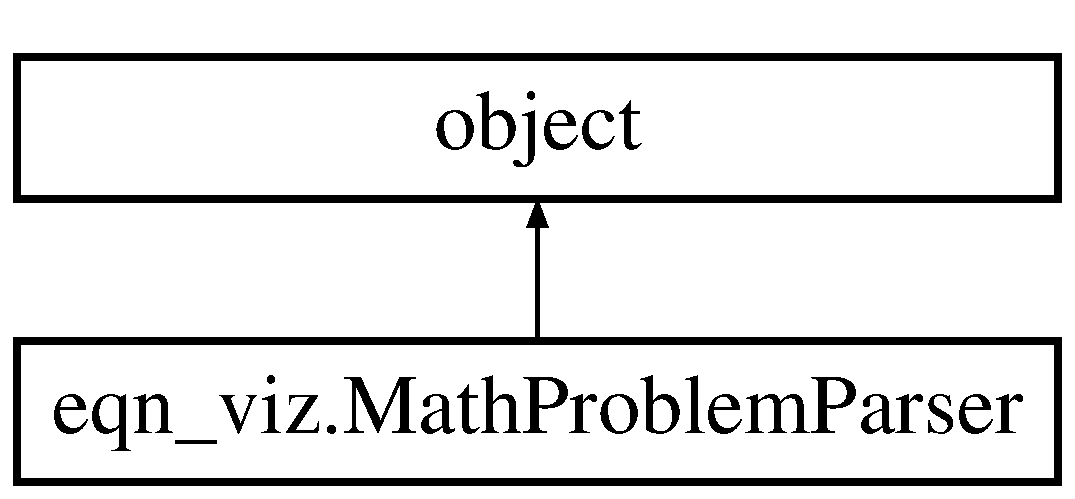
\includegraphics[height=2.000000cm]{classeqn__viz_1_1_math_problem_parser}
\end{center}
\end{figure}
\subsection*{Public Member Functions}
\begin{DoxyCompactItemize}
\item 
def \hyperlink{classeqn__viz_1_1_math_problem_parser_a2a21411a119d6a44fd67d010f452765d}{\+\_\+\+\_\+init\+\_\+\+\_\+}
\item 
def \hyperlink{classeqn__viz_1_1_math_problem_parser_a427749aff431b9838949ce868dd81621}{add\+Predicate} (self, time, pred\+\_\+array)
\item 
def \hyperlink{classeqn__viz_1_1_math_problem_parser_a127c28e9a12bbc78838891b2bbe85ef4}{get\+Solution\+String}
\item 
def \hyperlink{classeqn__viz_1_1_math_problem_parser_ae163bcbeaacca8c7e47af8d1a15fde8c}{add\+Action\+Pred} (self, step, action\+\_\+name)
\item 
def \hyperlink{classeqn__viz_1_1_math_problem_parser_ad7c8469e93c4c2f620f30d663f563c4b}{add\+Reference} (self, time\+\_\+step, pred\+\_\+num, node\+\_\+id)
\item 
def \hyperlink{classeqn__viz_1_1_math_problem_parser_ab05994e7b9a83931e5e0802b2c724261}{add\+Factor\+Pred} (self, time\+\_\+step, factor\+\_\+data)
\item 
def \hyperlink{classeqn__viz_1_1_math_problem_parser_ad1f35b057ba94c414bf18ff3eb414202}{add\+Operands} (self, time, operands)
\item 
def \hyperlink{classeqn__viz_1_1_math_problem_parser_a0e36a14a794a3612141dde4ddce4050d}{add\+Time} (self, time)
\item 
def \hyperlink{classeqn__viz_1_1_math_problem_parser_a71da891f047cb55a65759b22343f33e2}{get\+Problem} (self)
\item 
def \hyperlink{classeqn__viz_1_1_math_problem_parser_af59f19417ba8a05ef152b41e34c208eb}{get\+Operands} (self)
\item 
def \hyperlink{classeqn__viz_1_1_math_problem_parser_acaa8d2253504d12ee95cd79070289551}{get\+Eqn\+Steps} (self)
\item 
def \hyperlink{classeqn__viz_1_1_math_problem_parser_a4a4f4a6aa62b717dc159ec39ce25c35f}{use\+Y\+Variable} (self, \hyperlink{classeqn__viz_1_1_math_problem_parser_aa35a182df8bfc89e74a840e370e089f2}{solution\+\_\+steps})
\item 
def \hyperlink{classeqn__viz_1_1_math_problem_parser_adc7dee767cc96c729f3172cc399955a5}{append\+X\+Solutions} (self, \hyperlink{classeqn__viz_1_1_math_problem_parser_aa35a182df8bfc89e74a840e370e089f2}{solution\+\_\+steps})
\item 
def \hyperlink{classeqn__viz_1_1_math_problem_parser_a105702b6ef3f51d49153c51b1a5b1a29}{get\+Eqn\+Trees} (self)
\item 
def \hyperlink{classeqn__viz_1_1_math_problem_parser_aabf2f43b2ee403d9cf0cb873bbe28db9}{get\+Actions} (self)
\item 
def \hyperlink{classeqn__viz_1_1_math_problem_parser_a247aa12b6f38592c0fbcd0ac15b5520d}{get\+Explanations\+For\+Steps} (self)
\item 
def \hyperlink{classeqn__viz_1_1_math_problem_parser_af346d451472b46a9228c07d3dd7f0de8}{add\+Applicable\+Action} (self, action\+\_\+name)
\item 
def \hyperlink{classeqn__viz_1_1_math_problem_parser_aa8aded82942f9ac196e6e109fb9a45ec}{get\+Applicable\+Actions} (self)
\item 
def \hyperlink{classeqn__viz_1_1_math_problem_parser_a6adfec45bb22a5585db6e689c27aa393}{json\+Friendly\+Format} (self)
\end{DoxyCompactItemize}
\subsection*{Public Attributes}
\begin{DoxyCompactItemize}
\item 
\hyperlink{classeqn__viz_1_1_math_problem_parser_aa35a182df8bfc89e74a840e370e089f2}{solution\+\_\+steps}
\item 
\hyperlink{classeqn__viz_1_1_math_problem_parser_a3b02b0edd100ee6fd0b5b7d66bb22ecb}{actions}
\item 
\hyperlink{classeqn__viz_1_1_math_problem_parser_a09056a3b2b2490dccc4d3527c75c8f69}{applicable\+\_\+actions}
\item 
\hyperlink{classeqn__viz_1_1_math_problem_parser_a90141c1857b83a1bdfa5951453217204}{substitution\+\_\+happened}
\item 
\hyperlink{classeqn__viz_1_1_math_problem_parser_adda230f26ba7a90aa56f72e58a748c9e}{substitution\+\_\+degree}
\item 
\hyperlink{classeqn__viz_1_1_math_problem_parser_a6761399d080e0fd649cd5c2582590ccd}{substitution\+\_\+time\+\_\+step}
\item 
\hyperlink{classeqn__viz_1_1_math_problem_parser_ab84ba1169767799be1491b2baecb10ed}{solutions}
\end{DoxyCompactItemize}


\subsection{Detailed Description}
\begin{DoxyVerb}parse a single solution to a problem. This is done by adding
predicates one at a time to the parser, then calling 
getSolutionString().
\end{DoxyVerb}
 

Definition at line 395 of file eqn\+\_\+viz.\+py.



\subsection{Constructor \& Destructor Documentation}
\hypertarget{classeqn__viz_1_1_math_problem_parser_a2a21411a119d6a44fd67d010f452765d}{}\index{eqn\+\_\+viz\+::\+Math\+Problem\+Parser@{eqn\+\_\+viz\+::\+Math\+Problem\+Parser}!\+\_\+\+\_\+init\+\_\+\+\_\+@{\+\_\+\+\_\+init\+\_\+\+\_\+}}
\index{\+\_\+\+\_\+init\+\_\+\+\_\+@{\+\_\+\+\_\+init\+\_\+\+\_\+}!eqn\+\_\+viz\+::\+Math\+Problem\+Parser@{eqn\+\_\+viz\+::\+Math\+Problem\+Parser}}
\subsubsection[{\+\_\+\+\_\+init\+\_\+\+\_\+}]{\setlength{\rightskip}{0pt plus 5cm}def eqn\+\_\+viz.\+Math\+Problem\+Parser.\+\_\+\+\_\+init\+\_\+\+\_\+ (
\begin{DoxyParamCaption}
\item[{}]{self, }
\item[{}]{model\+\_\+mgr = {\ttfamily None}}
\end{DoxyParamCaption}
)}\label{classeqn__viz_1_1_math_problem_parser_a2a21411a119d6a44fd67d010f452765d}


Definition at line 401 of file eqn\+\_\+viz.\+py.



\subsection{Member Function Documentation}
\hypertarget{classeqn__viz_1_1_math_problem_parser_ae163bcbeaacca8c7e47af8d1a15fde8c}{}\index{eqn\+\_\+viz\+::\+Math\+Problem\+Parser@{eqn\+\_\+viz\+::\+Math\+Problem\+Parser}!add\+Action\+Pred@{add\+Action\+Pred}}
\index{add\+Action\+Pred@{add\+Action\+Pred}!eqn\+\_\+viz\+::\+Math\+Problem\+Parser@{eqn\+\_\+viz\+::\+Math\+Problem\+Parser}}
\subsubsection[{add\+Action\+Pred}]{\setlength{\rightskip}{0pt plus 5cm}def eqn\+\_\+viz.\+Math\+Problem\+Parser.\+add\+Action\+Pred (
\begin{DoxyParamCaption}
\item[{}]{self, }
\item[{}]{step, }
\item[{}]{action\+\_\+name}
\end{DoxyParamCaption}
)}\label{classeqn__viz_1_1_math_problem_parser_ae163bcbeaacca8c7e47af8d1a15fde8c}


Definition at line 428 of file eqn\+\_\+viz.\+py.

\hypertarget{classeqn__viz_1_1_math_problem_parser_af346d451472b46a9228c07d3dd7f0de8}{}\index{eqn\+\_\+viz\+::\+Math\+Problem\+Parser@{eqn\+\_\+viz\+::\+Math\+Problem\+Parser}!add\+Applicable\+Action@{add\+Applicable\+Action}}
\index{add\+Applicable\+Action@{add\+Applicable\+Action}!eqn\+\_\+viz\+::\+Math\+Problem\+Parser@{eqn\+\_\+viz\+::\+Math\+Problem\+Parser}}
\subsubsection[{add\+Applicable\+Action}]{\setlength{\rightskip}{0pt plus 5cm}def eqn\+\_\+viz.\+Math\+Problem\+Parser.\+add\+Applicable\+Action (
\begin{DoxyParamCaption}
\item[{}]{self, }
\item[{}]{action\+\_\+name}
\end{DoxyParamCaption}
)}\label{classeqn__viz_1_1_math_problem_parser_af346d451472b46a9228c07d3dd7f0de8}


Definition at line 484 of file eqn\+\_\+viz.\+py.

\hypertarget{classeqn__viz_1_1_math_problem_parser_ab05994e7b9a83931e5e0802b2c724261}{}\index{eqn\+\_\+viz\+::\+Math\+Problem\+Parser@{eqn\+\_\+viz\+::\+Math\+Problem\+Parser}!add\+Factor\+Pred@{add\+Factor\+Pred}}
\index{add\+Factor\+Pred@{add\+Factor\+Pred}!eqn\+\_\+viz\+::\+Math\+Problem\+Parser@{eqn\+\_\+viz\+::\+Math\+Problem\+Parser}}
\subsubsection[{add\+Factor\+Pred}]{\setlength{\rightskip}{0pt plus 5cm}def eqn\+\_\+viz.\+Math\+Problem\+Parser.\+add\+Factor\+Pred (
\begin{DoxyParamCaption}
\item[{}]{self, }
\item[{}]{time\+\_\+step, }
\item[{}]{factor\+\_\+data}
\end{DoxyParamCaption}
)}\label{classeqn__viz_1_1_math_problem_parser_ab05994e7b9a83931e5e0802b2c724261}


Definition at line 434 of file eqn\+\_\+viz.\+py.

\hypertarget{classeqn__viz_1_1_math_problem_parser_ad1f35b057ba94c414bf18ff3eb414202}{}\index{eqn\+\_\+viz\+::\+Math\+Problem\+Parser@{eqn\+\_\+viz\+::\+Math\+Problem\+Parser}!add\+Operands@{add\+Operands}}
\index{add\+Operands@{add\+Operands}!eqn\+\_\+viz\+::\+Math\+Problem\+Parser@{eqn\+\_\+viz\+::\+Math\+Problem\+Parser}}
\subsubsection[{add\+Operands}]{\setlength{\rightskip}{0pt plus 5cm}def eqn\+\_\+viz.\+Math\+Problem\+Parser.\+add\+Operands (
\begin{DoxyParamCaption}
\item[{}]{self, }
\item[{}]{time, }
\item[{}]{operands}
\end{DoxyParamCaption}
)}\label{classeqn__viz_1_1_math_problem_parser_ad1f35b057ba94c414bf18ff3eb414202}


Definition at line 436 of file eqn\+\_\+viz.\+py.

\hypertarget{classeqn__viz_1_1_math_problem_parser_a427749aff431b9838949ce868dd81621}{}\index{eqn\+\_\+viz\+::\+Math\+Problem\+Parser@{eqn\+\_\+viz\+::\+Math\+Problem\+Parser}!add\+Predicate@{add\+Predicate}}
\index{add\+Predicate@{add\+Predicate}!eqn\+\_\+viz\+::\+Math\+Problem\+Parser@{eqn\+\_\+viz\+::\+Math\+Problem\+Parser}}
\subsubsection[{add\+Predicate}]{\setlength{\rightskip}{0pt plus 5cm}def eqn\+\_\+viz.\+Math\+Problem\+Parser.\+add\+Predicate (
\begin{DoxyParamCaption}
\item[{}]{self, }
\item[{}]{time, }
\item[{}]{pred\+\_\+array}
\end{DoxyParamCaption}
)}\label{classeqn__viz_1_1_math_problem_parser_a427749aff431b9838949ce868dd81621}


Definition at line 410 of file eqn\+\_\+viz.\+py.

\hypertarget{classeqn__viz_1_1_math_problem_parser_ad7c8469e93c4c2f620f30d663f563c4b}{}\index{eqn\+\_\+viz\+::\+Math\+Problem\+Parser@{eqn\+\_\+viz\+::\+Math\+Problem\+Parser}!add\+Reference@{add\+Reference}}
\index{add\+Reference@{add\+Reference}!eqn\+\_\+viz\+::\+Math\+Problem\+Parser@{eqn\+\_\+viz\+::\+Math\+Problem\+Parser}}
\subsubsection[{add\+Reference}]{\setlength{\rightskip}{0pt plus 5cm}def eqn\+\_\+viz.\+Math\+Problem\+Parser.\+add\+Reference (
\begin{DoxyParamCaption}
\item[{}]{self, }
\item[{}]{time\+\_\+step, }
\item[{}]{pred\+\_\+num, }
\item[{}]{node\+\_\+id}
\end{DoxyParamCaption}
)}\label{classeqn__viz_1_1_math_problem_parser_ad7c8469e93c4c2f620f30d663f563c4b}


Definition at line 432 of file eqn\+\_\+viz.\+py.

\hypertarget{classeqn__viz_1_1_math_problem_parser_a0e36a14a794a3612141dde4ddce4050d}{}\index{eqn\+\_\+viz\+::\+Math\+Problem\+Parser@{eqn\+\_\+viz\+::\+Math\+Problem\+Parser}!add\+Time@{add\+Time}}
\index{add\+Time@{add\+Time}!eqn\+\_\+viz\+::\+Math\+Problem\+Parser@{eqn\+\_\+viz\+::\+Math\+Problem\+Parser}}
\subsubsection[{add\+Time}]{\setlength{\rightskip}{0pt plus 5cm}def eqn\+\_\+viz.\+Math\+Problem\+Parser.\+add\+Time (
\begin{DoxyParamCaption}
\item[{}]{self, }
\item[{}]{time}
\end{DoxyParamCaption}
)}\label{classeqn__viz_1_1_math_problem_parser_a0e36a14a794a3612141dde4ddce4050d}


Definition at line 439 of file eqn\+\_\+viz.\+py.

\hypertarget{classeqn__viz_1_1_math_problem_parser_adc7dee767cc96c729f3172cc399955a5}{}\index{eqn\+\_\+viz\+::\+Math\+Problem\+Parser@{eqn\+\_\+viz\+::\+Math\+Problem\+Parser}!append\+X\+Solutions@{append\+X\+Solutions}}
\index{append\+X\+Solutions@{append\+X\+Solutions}!eqn\+\_\+viz\+::\+Math\+Problem\+Parser@{eqn\+\_\+viz\+::\+Math\+Problem\+Parser}}
\subsubsection[{append\+X\+Solutions}]{\setlength{\rightskip}{0pt plus 5cm}def eqn\+\_\+viz.\+Math\+Problem\+Parser.\+append\+X\+Solutions (
\begin{DoxyParamCaption}
\item[{}]{self, }
\item[{}]{solution\+\_\+steps}
\end{DoxyParamCaption}
)}\label{classeqn__viz_1_1_math_problem_parser_adc7dee767cc96c729f3172cc399955a5}


Definition at line 460 of file eqn\+\_\+viz.\+py.

\hypertarget{classeqn__viz_1_1_math_problem_parser_aabf2f43b2ee403d9cf0cb873bbe28db9}{}\index{eqn\+\_\+viz\+::\+Math\+Problem\+Parser@{eqn\+\_\+viz\+::\+Math\+Problem\+Parser}!get\+Actions@{get\+Actions}}
\index{get\+Actions@{get\+Actions}!eqn\+\_\+viz\+::\+Math\+Problem\+Parser@{eqn\+\_\+viz\+::\+Math\+Problem\+Parser}}
\subsubsection[{get\+Actions}]{\setlength{\rightskip}{0pt plus 5cm}def eqn\+\_\+viz.\+Math\+Problem\+Parser.\+get\+Actions (
\begin{DoxyParamCaption}
\item[{}]{self}
\end{DoxyParamCaption}
)}\label{classeqn__viz_1_1_math_problem_parser_aabf2f43b2ee403d9cf0cb873bbe28db9}


Definition at line 474 of file eqn\+\_\+viz.\+py.

\hypertarget{classeqn__viz_1_1_math_problem_parser_aa8aded82942f9ac196e6e109fb9a45ec}{}\index{eqn\+\_\+viz\+::\+Math\+Problem\+Parser@{eqn\+\_\+viz\+::\+Math\+Problem\+Parser}!get\+Applicable\+Actions@{get\+Applicable\+Actions}}
\index{get\+Applicable\+Actions@{get\+Applicable\+Actions}!eqn\+\_\+viz\+::\+Math\+Problem\+Parser@{eqn\+\_\+viz\+::\+Math\+Problem\+Parser}}
\subsubsection[{get\+Applicable\+Actions}]{\setlength{\rightskip}{0pt plus 5cm}def eqn\+\_\+viz.\+Math\+Problem\+Parser.\+get\+Applicable\+Actions (
\begin{DoxyParamCaption}
\item[{}]{self}
\end{DoxyParamCaption}
)}\label{classeqn__viz_1_1_math_problem_parser_aa8aded82942f9ac196e6e109fb9a45ec}


Definition at line 486 of file eqn\+\_\+viz.\+py.

\hypertarget{classeqn__viz_1_1_math_problem_parser_acaa8d2253504d12ee95cd79070289551}{}\index{eqn\+\_\+viz\+::\+Math\+Problem\+Parser@{eqn\+\_\+viz\+::\+Math\+Problem\+Parser}!get\+Eqn\+Steps@{get\+Eqn\+Steps}}
\index{get\+Eqn\+Steps@{get\+Eqn\+Steps}!eqn\+\_\+viz\+::\+Math\+Problem\+Parser@{eqn\+\_\+viz\+::\+Math\+Problem\+Parser}}
\subsubsection[{get\+Eqn\+Steps}]{\setlength{\rightskip}{0pt plus 5cm}def eqn\+\_\+viz.\+Math\+Problem\+Parser.\+get\+Eqn\+Steps (
\begin{DoxyParamCaption}
\item[{}]{self}
\end{DoxyParamCaption}
)}\label{classeqn__viz_1_1_math_problem_parser_acaa8d2253504d12ee95cd79070289551}


Definition at line 446 of file eqn\+\_\+viz.\+py.

\hypertarget{classeqn__viz_1_1_math_problem_parser_a105702b6ef3f51d49153c51b1a5b1a29}{}\index{eqn\+\_\+viz\+::\+Math\+Problem\+Parser@{eqn\+\_\+viz\+::\+Math\+Problem\+Parser}!get\+Eqn\+Trees@{get\+Eqn\+Trees}}
\index{get\+Eqn\+Trees@{get\+Eqn\+Trees}!eqn\+\_\+viz\+::\+Math\+Problem\+Parser@{eqn\+\_\+viz\+::\+Math\+Problem\+Parser}}
\subsubsection[{get\+Eqn\+Trees}]{\setlength{\rightskip}{0pt plus 5cm}def eqn\+\_\+viz.\+Math\+Problem\+Parser.\+get\+Eqn\+Trees (
\begin{DoxyParamCaption}
\item[{}]{self}
\end{DoxyParamCaption}
)}\label{classeqn__viz_1_1_math_problem_parser_a105702b6ef3f51d49153c51b1a5b1a29}


Definition at line 472 of file eqn\+\_\+viz.\+py.

\hypertarget{classeqn__viz_1_1_math_problem_parser_a247aa12b6f38592c0fbcd0ac15b5520d}{}\index{eqn\+\_\+viz\+::\+Math\+Problem\+Parser@{eqn\+\_\+viz\+::\+Math\+Problem\+Parser}!get\+Explanations\+For\+Steps@{get\+Explanations\+For\+Steps}}
\index{get\+Explanations\+For\+Steps@{get\+Explanations\+For\+Steps}!eqn\+\_\+viz\+::\+Math\+Problem\+Parser@{eqn\+\_\+viz\+::\+Math\+Problem\+Parser}}
\subsubsection[{get\+Explanations\+For\+Steps}]{\setlength{\rightskip}{0pt plus 5cm}def eqn\+\_\+viz.\+Math\+Problem\+Parser.\+get\+Explanations\+For\+Steps (
\begin{DoxyParamCaption}
\item[{}]{self}
\end{DoxyParamCaption}
)}\label{classeqn__viz_1_1_math_problem_parser_a247aa12b6f38592c0fbcd0ac15b5520d}


Definition at line 477 of file eqn\+\_\+viz.\+py.

\hypertarget{classeqn__viz_1_1_math_problem_parser_af59f19417ba8a05ef152b41e34c208eb}{}\index{eqn\+\_\+viz\+::\+Math\+Problem\+Parser@{eqn\+\_\+viz\+::\+Math\+Problem\+Parser}!get\+Operands@{get\+Operands}}
\index{get\+Operands@{get\+Operands}!eqn\+\_\+viz\+::\+Math\+Problem\+Parser@{eqn\+\_\+viz\+::\+Math\+Problem\+Parser}}
\subsubsection[{get\+Operands}]{\setlength{\rightskip}{0pt plus 5cm}def eqn\+\_\+viz.\+Math\+Problem\+Parser.\+get\+Operands (
\begin{DoxyParamCaption}
\item[{}]{self}
\end{DoxyParamCaption}
)}\label{classeqn__viz_1_1_math_problem_parser_af59f19417ba8a05ef152b41e34c208eb}


Definition at line 444 of file eqn\+\_\+viz.\+py.

\hypertarget{classeqn__viz_1_1_math_problem_parser_a71da891f047cb55a65759b22343f33e2}{}\index{eqn\+\_\+viz\+::\+Math\+Problem\+Parser@{eqn\+\_\+viz\+::\+Math\+Problem\+Parser}!get\+Problem@{get\+Problem}}
\index{get\+Problem@{get\+Problem}!eqn\+\_\+viz\+::\+Math\+Problem\+Parser@{eqn\+\_\+viz\+::\+Math\+Problem\+Parser}}
\subsubsection[{get\+Problem}]{\setlength{\rightskip}{0pt plus 5cm}def eqn\+\_\+viz.\+Math\+Problem\+Parser.\+get\+Problem (
\begin{DoxyParamCaption}
\item[{}]{self}
\end{DoxyParamCaption}
)}\label{classeqn__viz_1_1_math_problem_parser_a71da891f047cb55a65759b22343f33e2}


Definition at line 442 of file eqn\+\_\+viz.\+py.

\hypertarget{classeqn__viz_1_1_math_problem_parser_a127c28e9a12bbc78838891b2bbe85ef4}{}\index{eqn\+\_\+viz\+::\+Math\+Problem\+Parser@{eqn\+\_\+viz\+::\+Math\+Problem\+Parser}!get\+Solution\+String@{get\+Solution\+String}}
\index{get\+Solution\+String@{get\+Solution\+String}!eqn\+\_\+viz\+::\+Math\+Problem\+Parser@{eqn\+\_\+viz\+::\+Math\+Problem\+Parser}}
\subsubsection[{get\+Solution\+String}]{\setlength{\rightskip}{0pt plus 5cm}def eqn\+\_\+viz.\+Math\+Problem\+Parser.\+get\+Solution\+String (
\begin{DoxyParamCaption}
\item[{}]{self, }
\item[{}]{as\+\_\+latex = {\ttfamily False}, }
\item[{}]{json\+\_\+output = {\ttfamily False}}
\end{DoxyParamCaption}
)}\label{classeqn__viz_1_1_math_problem_parser_a127c28e9a12bbc78838891b2bbe85ef4}


Definition at line 413 of file eqn\+\_\+viz.\+py.

\hypertarget{classeqn__viz_1_1_math_problem_parser_a6adfec45bb22a5585db6e689c27aa393}{}\index{eqn\+\_\+viz\+::\+Math\+Problem\+Parser@{eqn\+\_\+viz\+::\+Math\+Problem\+Parser}!json\+Friendly\+Format@{json\+Friendly\+Format}}
\index{json\+Friendly\+Format@{json\+Friendly\+Format}!eqn\+\_\+viz\+::\+Math\+Problem\+Parser@{eqn\+\_\+viz\+::\+Math\+Problem\+Parser}}
\subsubsection[{json\+Friendly\+Format}]{\setlength{\rightskip}{0pt plus 5cm}def eqn\+\_\+viz.\+Math\+Problem\+Parser.\+json\+Friendly\+Format (
\begin{DoxyParamCaption}
\item[{}]{self}
\end{DoxyParamCaption}
)}\label{classeqn__viz_1_1_math_problem_parser_a6adfec45bb22a5585db6e689c27aa393}


Definition at line 488 of file eqn\+\_\+viz.\+py.

\hypertarget{classeqn__viz_1_1_math_problem_parser_a4a4f4a6aa62b717dc159ec39ce25c35f}{}\index{eqn\+\_\+viz\+::\+Math\+Problem\+Parser@{eqn\+\_\+viz\+::\+Math\+Problem\+Parser}!use\+Y\+Variable@{use\+Y\+Variable}}
\index{use\+Y\+Variable@{use\+Y\+Variable}!eqn\+\_\+viz\+::\+Math\+Problem\+Parser@{eqn\+\_\+viz\+::\+Math\+Problem\+Parser}}
\subsubsection[{use\+Y\+Variable}]{\setlength{\rightskip}{0pt plus 5cm}def eqn\+\_\+viz.\+Math\+Problem\+Parser.\+use\+Y\+Variable (
\begin{DoxyParamCaption}
\item[{}]{self, }
\item[{}]{solution\+\_\+steps}
\end{DoxyParamCaption}
)}\label{classeqn__viz_1_1_math_problem_parser_a4a4f4a6aa62b717dc159ec39ce25c35f}


Definition at line 452 of file eqn\+\_\+viz.\+py.



\subsection{Member Data Documentation}
\hypertarget{classeqn__viz_1_1_math_problem_parser_a3b02b0edd100ee6fd0b5b7d66bb22ecb}{}\index{eqn\+\_\+viz\+::\+Math\+Problem\+Parser@{eqn\+\_\+viz\+::\+Math\+Problem\+Parser}!actions@{actions}}
\index{actions@{actions}!eqn\+\_\+viz\+::\+Math\+Problem\+Parser@{eqn\+\_\+viz\+::\+Math\+Problem\+Parser}}
\subsubsection[{actions}]{\setlength{\rightskip}{0pt plus 5cm}eqn\+\_\+viz.\+Math\+Problem\+Parser.\+actions}\label{classeqn__viz_1_1_math_problem_parser_a3b02b0edd100ee6fd0b5b7d66bb22ecb}


Definition at line 403 of file eqn\+\_\+viz.\+py.

\hypertarget{classeqn__viz_1_1_math_problem_parser_a09056a3b2b2490dccc4d3527c75c8f69}{}\index{eqn\+\_\+viz\+::\+Math\+Problem\+Parser@{eqn\+\_\+viz\+::\+Math\+Problem\+Parser}!applicable\+\_\+actions@{applicable\+\_\+actions}}
\index{applicable\+\_\+actions@{applicable\+\_\+actions}!eqn\+\_\+viz\+::\+Math\+Problem\+Parser@{eqn\+\_\+viz\+::\+Math\+Problem\+Parser}}
\subsubsection[{applicable\+\_\+actions}]{\setlength{\rightskip}{0pt plus 5cm}eqn\+\_\+viz.\+Math\+Problem\+Parser.\+applicable\+\_\+actions}\label{classeqn__viz_1_1_math_problem_parser_a09056a3b2b2490dccc4d3527c75c8f69}


Definition at line 404 of file eqn\+\_\+viz.\+py.

\hypertarget{classeqn__viz_1_1_math_problem_parser_aa35a182df8bfc89e74a840e370e089f2}{}\index{eqn\+\_\+viz\+::\+Math\+Problem\+Parser@{eqn\+\_\+viz\+::\+Math\+Problem\+Parser}!solution\+\_\+steps@{solution\+\_\+steps}}
\index{solution\+\_\+steps@{solution\+\_\+steps}!eqn\+\_\+viz\+::\+Math\+Problem\+Parser@{eqn\+\_\+viz\+::\+Math\+Problem\+Parser}}
\subsubsection[{solution\+\_\+steps}]{\setlength{\rightskip}{0pt plus 5cm}eqn\+\_\+viz.\+Math\+Problem\+Parser.\+solution\+\_\+steps}\label{classeqn__viz_1_1_math_problem_parser_aa35a182df8bfc89e74a840e370e089f2}


Definition at line 402 of file eqn\+\_\+viz.\+py.

\hypertarget{classeqn__viz_1_1_math_problem_parser_ab84ba1169767799be1491b2baecb10ed}{}\index{eqn\+\_\+viz\+::\+Math\+Problem\+Parser@{eqn\+\_\+viz\+::\+Math\+Problem\+Parser}!solutions@{solutions}}
\index{solutions@{solutions}!eqn\+\_\+viz\+::\+Math\+Problem\+Parser@{eqn\+\_\+viz\+::\+Math\+Problem\+Parser}}
\subsubsection[{solutions}]{\setlength{\rightskip}{0pt plus 5cm}eqn\+\_\+viz.\+Math\+Problem\+Parser.\+solutions}\label{classeqn__viz_1_1_math_problem_parser_ab84ba1169767799be1491b2baecb10ed}


Definition at line 409 of file eqn\+\_\+viz.\+py.

\hypertarget{classeqn__viz_1_1_math_problem_parser_adda230f26ba7a90aa56f72e58a748c9e}{}\index{eqn\+\_\+viz\+::\+Math\+Problem\+Parser@{eqn\+\_\+viz\+::\+Math\+Problem\+Parser}!substitution\+\_\+degree@{substitution\+\_\+degree}}
\index{substitution\+\_\+degree@{substitution\+\_\+degree}!eqn\+\_\+viz\+::\+Math\+Problem\+Parser@{eqn\+\_\+viz\+::\+Math\+Problem\+Parser}}
\subsubsection[{substitution\+\_\+degree}]{\setlength{\rightskip}{0pt plus 5cm}eqn\+\_\+viz.\+Math\+Problem\+Parser.\+substitution\+\_\+degree}\label{classeqn__viz_1_1_math_problem_parser_adda230f26ba7a90aa56f72e58a748c9e}


Definition at line 407 of file eqn\+\_\+viz.\+py.

\hypertarget{classeqn__viz_1_1_math_problem_parser_a90141c1857b83a1bdfa5951453217204}{}\index{eqn\+\_\+viz\+::\+Math\+Problem\+Parser@{eqn\+\_\+viz\+::\+Math\+Problem\+Parser}!substitution\+\_\+happened@{substitution\+\_\+happened}}
\index{substitution\+\_\+happened@{substitution\+\_\+happened}!eqn\+\_\+viz\+::\+Math\+Problem\+Parser@{eqn\+\_\+viz\+::\+Math\+Problem\+Parser}}
\subsubsection[{substitution\+\_\+happened}]{\setlength{\rightskip}{0pt plus 5cm}eqn\+\_\+viz.\+Math\+Problem\+Parser.\+substitution\+\_\+happened}\label{classeqn__viz_1_1_math_problem_parser_a90141c1857b83a1bdfa5951453217204}


Definition at line 406 of file eqn\+\_\+viz.\+py.

\hypertarget{classeqn__viz_1_1_math_problem_parser_a6761399d080e0fd649cd5c2582590ccd}{}\index{eqn\+\_\+viz\+::\+Math\+Problem\+Parser@{eqn\+\_\+viz\+::\+Math\+Problem\+Parser}!substitution\+\_\+time\+\_\+step@{substitution\+\_\+time\+\_\+step}}
\index{substitution\+\_\+time\+\_\+step@{substitution\+\_\+time\+\_\+step}!eqn\+\_\+viz\+::\+Math\+Problem\+Parser@{eqn\+\_\+viz\+::\+Math\+Problem\+Parser}}
\subsubsection[{substitution\+\_\+time\+\_\+step}]{\setlength{\rightskip}{0pt plus 5cm}eqn\+\_\+viz.\+Math\+Problem\+Parser.\+substitution\+\_\+time\+\_\+step}\label{classeqn__viz_1_1_math_problem_parser_a6761399d080e0fd649cd5c2582590ccd}


Definition at line 408 of file eqn\+\_\+viz.\+py.



The documentation for this class was generated from the following file\+:\begin{DoxyCompactItemize}
\item 
\hyperlink{eqn__viz_8py}{eqn\+\_\+viz.\+py}\end{DoxyCompactItemize}

\hypertarget{classmodel__manager_1_1_model_manager}{}\section{model\+\_\+manager.\+Model\+Manager Class Reference}
\label{classmodel__manager_1_1_model_manager}\index{model\+\_\+manager.\+Model\+Manager@{model\+\_\+manager.\+Model\+Manager}}
Inheritance diagram for model\+\_\+manager.\+Model\+Manager\+:\begin{figure}[H]
\begin{center}
\leavevmode
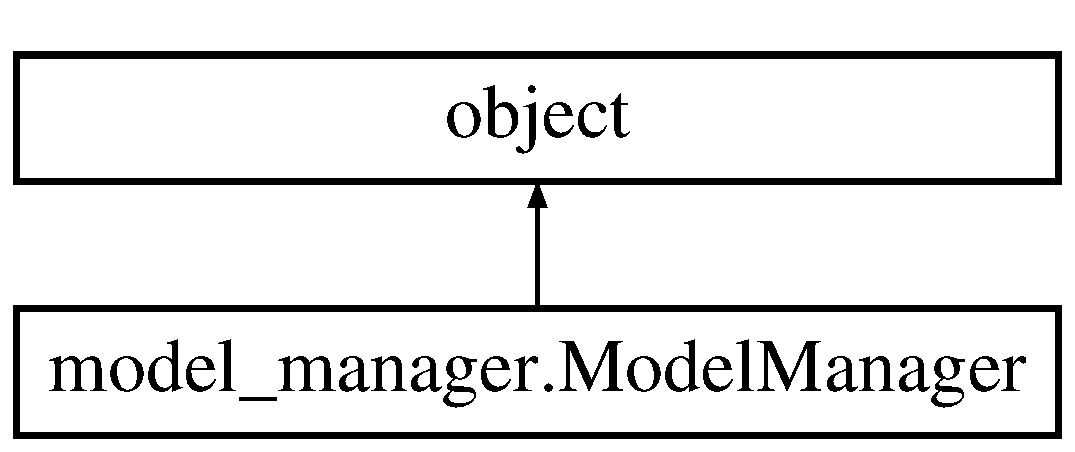
\includegraphics[height=2.000000cm]{classmodel__manager_1_1_model_manager}
\end{center}
\end{figure}
\subsection*{Public Member Functions}
\begin{DoxyCompactItemize}
\item 
def \hyperlink{classmodel__manager_1_1_model_manager_ac4022bf288503dbe0c4244bd6030665a}{\+\_\+\+\_\+init\+\_\+\+\_\+} (self)
\item 
def \hyperlink{classmodel__manager_1_1_model_manager_a8ee1b63e780706cf70c09771b394ad74}{add\+Predicate} (self, predicate\+\_\+string)
\item 
def \hyperlink{classmodel__manager_1_1_model_manager_a5b455d9f9ea6fd8fe8929e5c0722cf40}{unify} (self, pred\+\_\+key, partial\+\_\+assign)
\item 
def \hyperlink{classmodel__manager_1_1_model_manager_ac655a140d67621098366316e8615b7a8}{matches} (self, grounding, partial\+\_\+assign)
\item 
def \hyperlink{classmodel__manager_1_1_model_manager_adaf953996847c9994f329949b31aacdd}{print\+Model} (self)
\item 
def \hyperlink{classmodel__manager_1_1_model_manager_ac3ed4387e5e5d451bc8f145192f43251}{get\+All\+Ground\+Instances\+Of} (self, pred\+\_\+key)
\end{DoxyCompactItemize}
\subsection*{Static Public Member Functions}
\begin{DoxyCompactItemize}
\item 
def \hyperlink{classmodel__manager_1_1_model_manager_a36cc10dbad36fe9d92633cbef7a94a20}{split\+Predicate} (pred\+\_\+string)
\end{DoxyCompactItemize}
\subsection*{Public Attributes}
\begin{DoxyCompactItemize}
\item 
\hyperlink{classmodel__manager_1_1_model_manager_af557b050f1181ef829814605a35fdad0}{model\+\_\+predicates}
\end{DoxyCompactItemize}


\subsection{Detailed Description}
\begin{DoxyVerb}records every atom for a generated model (answer set)\end{DoxyVerb}
 

Definition at line 10 of file model\+\_\+manager.\+py.



\subsection{Constructor \& Destructor Documentation}
\hypertarget{classmodel__manager_1_1_model_manager_ac4022bf288503dbe0c4244bd6030665a}{}\index{model\+\_\+manager\+::\+Model\+Manager@{model\+\_\+manager\+::\+Model\+Manager}!\+\_\+\+\_\+init\+\_\+\+\_\+@{\+\_\+\+\_\+init\+\_\+\+\_\+}}
\index{\+\_\+\+\_\+init\+\_\+\+\_\+@{\+\_\+\+\_\+init\+\_\+\+\_\+}!model\+\_\+manager\+::\+Model\+Manager@{model\+\_\+manager\+::\+Model\+Manager}}
\subsubsection[{\+\_\+\+\_\+init\+\_\+\+\_\+}]{\setlength{\rightskip}{0pt plus 5cm}def model\+\_\+manager.\+Model\+Manager.\+\_\+\+\_\+init\+\_\+\+\_\+ (
\begin{DoxyParamCaption}
\item[{}]{self}
\end{DoxyParamCaption}
)}\label{classmodel__manager_1_1_model_manager_ac4022bf288503dbe0c4244bd6030665a}


Definition at line 13 of file model\+\_\+manager.\+py.



\subsection{Member Function Documentation}
\hypertarget{classmodel__manager_1_1_model_manager_a8ee1b63e780706cf70c09771b394ad74}{}\index{model\+\_\+manager\+::\+Model\+Manager@{model\+\_\+manager\+::\+Model\+Manager}!add\+Predicate@{add\+Predicate}}
\index{add\+Predicate@{add\+Predicate}!model\+\_\+manager\+::\+Model\+Manager@{model\+\_\+manager\+::\+Model\+Manager}}
\subsubsection[{add\+Predicate}]{\setlength{\rightskip}{0pt plus 5cm}def model\+\_\+manager.\+Model\+Manager.\+add\+Predicate (
\begin{DoxyParamCaption}
\item[{}]{self, }
\item[{}]{predicate\+\_\+string}
\end{DoxyParamCaption}
)}\label{classmodel__manager_1_1_model_manager_a8ee1b63e780706cf70c09771b394ad74}
\begin{DoxyVerb}add grounded predicate to model\end{DoxyVerb}
 

Definition at line 16 of file model\+\_\+manager.\+py.

\hypertarget{classmodel__manager_1_1_model_manager_ac3ed4387e5e5d451bc8f145192f43251}{}\index{model\+\_\+manager\+::\+Model\+Manager@{model\+\_\+manager\+::\+Model\+Manager}!get\+All\+Ground\+Instances\+Of@{get\+All\+Ground\+Instances\+Of}}
\index{get\+All\+Ground\+Instances\+Of@{get\+All\+Ground\+Instances\+Of}!model\+\_\+manager\+::\+Model\+Manager@{model\+\_\+manager\+::\+Model\+Manager}}
\subsubsection[{get\+All\+Ground\+Instances\+Of}]{\setlength{\rightskip}{0pt plus 5cm}def model\+\_\+manager.\+Model\+Manager.\+get\+All\+Ground\+Instances\+Of (
\begin{DoxyParamCaption}
\item[{}]{self, }
\item[{}]{pred\+\_\+key}
\end{DoxyParamCaption}
)}\label{classmodel__manager_1_1_model_manager_ac3ed4387e5e5d451bc8f145192f43251}


Definition at line 80 of file model\+\_\+manager.\+py.

\hypertarget{classmodel__manager_1_1_model_manager_ac655a140d67621098366316e8615b7a8}{}\index{model\+\_\+manager\+::\+Model\+Manager@{model\+\_\+manager\+::\+Model\+Manager}!matches@{matches}}
\index{matches@{matches}!model\+\_\+manager\+::\+Model\+Manager@{model\+\_\+manager\+::\+Model\+Manager}}
\subsubsection[{matches}]{\setlength{\rightskip}{0pt plus 5cm}def model\+\_\+manager.\+Model\+Manager.\+matches (
\begin{DoxyParamCaption}
\item[{}]{self, }
\item[{}]{grounding, }
\item[{}]{partial\+\_\+assign}
\end{DoxyParamCaption}
)}\label{classmodel__manager_1_1_model_manager_ac655a140d67621098366316e8615b7a8}


Definition at line 28 of file model\+\_\+manager.\+py.

\hypertarget{classmodel__manager_1_1_model_manager_adaf953996847c9994f329949b31aacdd}{}\index{model\+\_\+manager\+::\+Model\+Manager@{model\+\_\+manager\+::\+Model\+Manager}!print\+Model@{print\+Model}}
\index{print\+Model@{print\+Model}!model\+\_\+manager\+::\+Model\+Manager@{model\+\_\+manager\+::\+Model\+Manager}}
\subsubsection[{print\+Model}]{\setlength{\rightskip}{0pt plus 5cm}def model\+\_\+manager.\+Model\+Manager.\+print\+Model (
\begin{DoxyParamCaption}
\item[{}]{self}
\end{DoxyParamCaption}
)}\label{classmodel__manager_1_1_model_manager_adaf953996847c9994f329949b31aacdd}


Definition at line 33 of file model\+\_\+manager.\+py.

\hypertarget{classmodel__manager_1_1_model_manager_a36cc10dbad36fe9d92633cbef7a94a20}{}\index{model\+\_\+manager\+::\+Model\+Manager@{model\+\_\+manager\+::\+Model\+Manager}!split\+Predicate@{split\+Predicate}}
\index{split\+Predicate@{split\+Predicate}!model\+\_\+manager\+::\+Model\+Manager@{model\+\_\+manager\+::\+Model\+Manager}}
\subsubsection[{split\+Predicate}]{\setlength{\rightskip}{0pt plus 5cm}def model\+\_\+manager.\+Model\+Manager.\+split\+Predicate (
\begin{DoxyParamCaption}
\item[{}]{pred\+\_\+string}
\end{DoxyParamCaption}
)\hspace{0.3cm}{\ttfamily [static]}}\label{classmodel__manager_1_1_model_manager_a36cc10dbad36fe9d92633cbef7a94a20}
\begin{DoxyVerb}return predicate name and list of operands from predicate string\end{DoxyVerb}
 

Definition at line 40 of file model\+\_\+manager.\+py.

\hypertarget{classmodel__manager_1_1_model_manager_a5b455d9f9ea6fd8fe8929e5c0722cf40}{}\index{model\+\_\+manager\+::\+Model\+Manager@{model\+\_\+manager\+::\+Model\+Manager}!unify@{unify}}
\index{unify@{unify}!model\+\_\+manager\+::\+Model\+Manager@{model\+\_\+manager\+::\+Model\+Manager}}
\subsubsection[{unify}]{\setlength{\rightskip}{0pt plus 5cm}def model\+\_\+manager.\+Model\+Manager.\+unify (
\begin{DoxyParamCaption}
\item[{}]{self, }
\item[{}]{pred\+\_\+key, }
\item[{}]{partial\+\_\+assign}
\end{DoxyParamCaption}
)}\label{classmodel__manager_1_1_model_manager_a5b455d9f9ea6fd8fe8929e5c0722cf40}


Definition at line 22 of file model\+\_\+manager.\+py.



\subsection{Member Data Documentation}
\hypertarget{classmodel__manager_1_1_model_manager_af557b050f1181ef829814605a35fdad0}{}\index{model\+\_\+manager\+::\+Model\+Manager@{model\+\_\+manager\+::\+Model\+Manager}!model\+\_\+predicates@{model\+\_\+predicates}}
\index{model\+\_\+predicates@{model\+\_\+predicates}!model\+\_\+manager\+::\+Model\+Manager@{model\+\_\+manager\+::\+Model\+Manager}}
\subsubsection[{model\+\_\+predicates}]{\setlength{\rightskip}{0pt plus 5cm}model\+\_\+manager.\+Model\+Manager.\+model\+\_\+predicates}\label{classmodel__manager_1_1_model_manager_af557b050f1181ef829814605a35fdad0}


Definition at line 15 of file model\+\_\+manager.\+py.



The documentation for this class was generated from the following file\+:\begin{DoxyCompactItemize}
\item 
\hyperlink{model__manager_8py}{model\+\_\+manager.\+py}\end{DoxyCompactItemize}

\hypertarget{classeqn__viz_1_1_model_manager}{}\section{eqn\+\_\+viz.\+Model\+Manager Class Reference}
\label{classeqn__viz_1_1_model_manager}\index{eqn\+\_\+viz.\+Model\+Manager@{eqn\+\_\+viz.\+Model\+Manager}}
Inheritance diagram for eqn\+\_\+viz.\+Model\+Manager\+:\begin{figure}[H]
\begin{center}
\leavevmode
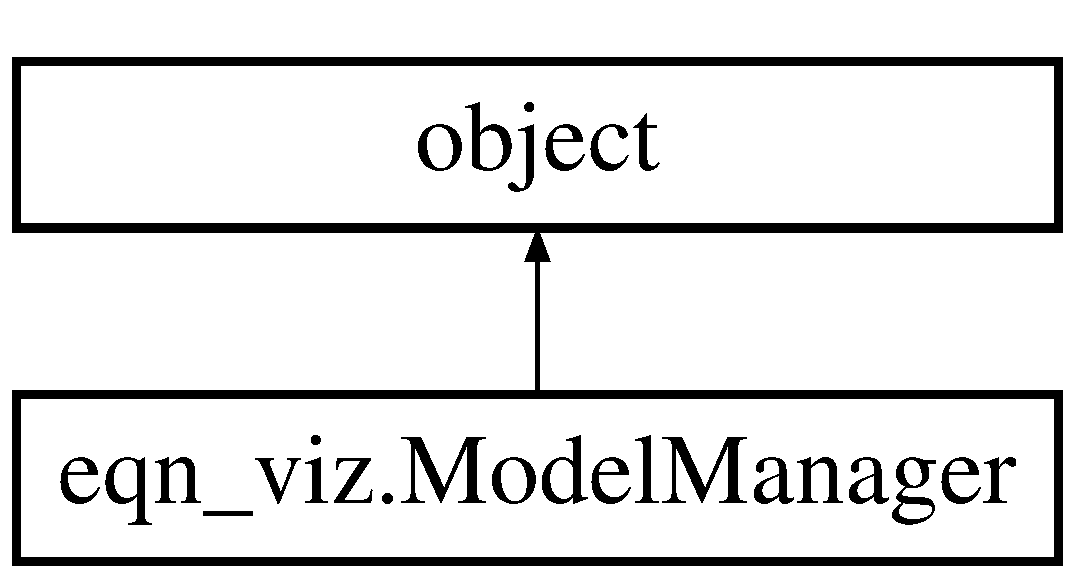
\includegraphics[height=2.000000cm]{classeqn__viz_1_1_model_manager}
\end{center}
\end{figure}
\subsection*{Public Member Functions}
\begin{DoxyCompactItemize}
\item 
def \hyperlink{classeqn__viz_1_1_model_manager_af6ba57e4dc5a80892675666f43c684f0}{\+\_\+\+\_\+init\+\_\+\+\_\+} (self)
\item 
def \hyperlink{classeqn__viz_1_1_model_manager_ac48c7611f5a1fe95415e0651e25a178c}{add\+Predicate} (self, predicate\+\_\+string)
\item 
def \hyperlink{classeqn__viz_1_1_model_manager_ab8c6e9a67b3c5d03195a51b252279803}{unify} (self, pred\+\_\+key, partial\+\_\+assign)
\item 
def \hyperlink{classeqn__viz_1_1_model_manager_af8a8903380fb509db8188c7ad91e3d3c}{matches} (self, grounding, partial\+\_\+assign)
\item 
def \hyperlink{classeqn__viz_1_1_model_manager_a8cdf7c43e933d043dd25cd2fd76b4836}{print\+Model} (self)
\end{DoxyCompactItemize}
\subsection*{Static Public Member Functions}
\begin{DoxyCompactItemize}
\item 
def \hyperlink{classeqn__viz_1_1_model_manager_a01de2c06921a956c3ccf1f64e3fc1c77}{split\+Predicate} (pred\+\_\+string)
\end{DoxyCompactItemize}
\subsection*{Public Attributes}
\begin{DoxyCompactItemize}
\item 
\hyperlink{classeqn__viz_1_1_model_manager_a6b199994d8ecef6d3f7ccfa73bcabd04}{model\+\_\+predicates}
\end{DoxyCompactItemize}


\subsection{Detailed Description}
\begin{DoxyVerb}records every atom for a generated model (answer set)\end{DoxyVerb}
 

Definition at line 498 of file eqn\+\_\+viz.\+py.



\subsection{Constructor \& Destructor Documentation}
\hypertarget{classeqn__viz_1_1_model_manager_af6ba57e4dc5a80892675666f43c684f0}{}\index{eqn\+\_\+viz\+::\+Model\+Manager@{eqn\+\_\+viz\+::\+Model\+Manager}!\+\_\+\+\_\+init\+\_\+\+\_\+@{\+\_\+\+\_\+init\+\_\+\+\_\+}}
\index{\+\_\+\+\_\+init\+\_\+\+\_\+@{\+\_\+\+\_\+init\+\_\+\+\_\+}!eqn\+\_\+viz\+::\+Model\+Manager@{eqn\+\_\+viz\+::\+Model\+Manager}}
\subsubsection[{\+\_\+\+\_\+init\+\_\+\+\_\+}]{\setlength{\rightskip}{0pt plus 5cm}def eqn\+\_\+viz.\+Model\+Manager.\+\_\+\+\_\+init\+\_\+\+\_\+ (
\begin{DoxyParamCaption}
\item[{}]{self}
\end{DoxyParamCaption}
)}\label{classeqn__viz_1_1_model_manager_af6ba57e4dc5a80892675666f43c684f0}


Definition at line 501 of file eqn\+\_\+viz.\+py.



\subsection{Member Function Documentation}
\hypertarget{classeqn__viz_1_1_model_manager_ac48c7611f5a1fe95415e0651e25a178c}{}\index{eqn\+\_\+viz\+::\+Model\+Manager@{eqn\+\_\+viz\+::\+Model\+Manager}!add\+Predicate@{add\+Predicate}}
\index{add\+Predicate@{add\+Predicate}!eqn\+\_\+viz\+::\+Model\+Manager@{eqn\+\_\+viz\+::\+Model\+Manager}}
\subsubsection[{add\+Predicate}]{\setlength{\rightskip}{0pt plus 5cm}def eqn\+\_\+viz.\+Model\+Manager.\+add\+Predicate (
\begin{DoxyParamCaption}
\item[{}]{self, }
\item[{}]{predicate\+\_\+string}
\end{DoxyParamCaption}
)}\label{classeqn__viz_1_1_model_manager_ac48c7611f5a1fe95415e0651e25a178c}
\begin{DoxyVerb}add grounded predicate to model\end{DoxyVerb}
 

Definition at line 504 of file eqn\+\_\+viz.\+py.

\hypertarget{classeqn__viz_1_1_model_manager_af8a8903380fb509db8188c7ad91e3d3c}{}\index{eqn\+\_\+viz\+::\+Model\+Manager@{eqn\+\_\+viz\+::\+Model\+Manager}!matches@{matches}}
\index{matches@{matches}!eqn\+\_\+viz\+::\+Model\+Manager@{eqn\+\_\+viz\+::\+Model\+Manager}}
\subsubsection[{matches}]{\setlength{\rightskip}{0pt plus 5cm}def eqn\+\_\+viz.\+Model\+Manager.\+matches (
\begin{DoxyParamCaption}
\item[{}]{self, }
\item[{}]{grounding, }
\item[{}]{partial\+\_\+assign}
\end{DoxyParamCaption}
)}\label{classeqn__viz_1_1_model_manager_af8a8903380fb509db8188c7ad91e3d3c}


Definition at line 516 of file eqn\+\_\+viz.\+py.

\hypertarget{classeqn__viz_1_1_model_manager_a8cdf7c43e933d043dd25cd2fd76b4836}{}\index{eqn\+\_\+viz\+::\+Model\+Manager@{eqn\+\_\+viz\+::\+Model\+Manager}!print\+Model@{print\+Model}}
\index{print\+Model@{print\+Model}!eqn\+\_\+viz\+::\+Model\+Manager@{eqn\+\_\+viz\+::\+Model\+Manager}}
\subsubsection[{print\+Model}]{\setlength{\rightskip}{0pt plus 5cm}def eqn\+\_\+viz.\+Model\+Manager.\+print\+Model (
\begin{DoxyParamCaption}
\item[{}]{self}
\end{DoxyParamCaption}
)}\label{classeqn__viz_1_1_model_manager_a8cdf7c43e933d043dd25cd2fd76b4836}


Definition at line 521 of file eqn\+\_\+viz.\+py.

\hypertarget{classeqn__viz_1_1_model_manager_a01de2c06921a956c3ccf1f64e3fc1c77}{}\index{eqn\+\_\+viz\+::\+Model\+Manager@{eqn\+\_\+viz\+::\+Model\+Manager}!split\+Predicate@{split\+Predicate}}
\index{split\+Predicate@{split\+Predicate}!eqn\+\_\+viz\+::\+Model\+Manager@{eqn\+\_\+viz\+::\+Model\+Manager}}
\subsubsection[{split\+Predicate}]{\setlength{\rightskip}{0pt plus 5cm}def eqn\+\_\+viz.\+Model\+Manager.\+split\+Predicate (
\begin{DoxyParamCaption}
\item[{}]{pred\+\_\+string}
\end{DoxyParamCaption}
)\hspace{0.3cm}{\ttfamily [static]}}\label{classeqn__viz_1_1_model_manager_a01de2c06921a956c3ccf1f64e3fc1c77}
\begin{DoxyVerb}return predicate name and list of operands from predicate string\end{DoxyVerb}
 

Definition at line 528 of file eqn\+\_\+viz.\+py.

\hypertarget{classeqn__viz_1_1_model_manager_ab8c6e9a67b3c5d03195a51b252279803}{}\index{eqn\+\_\+viz\+::\+Model\+Manager@{eqn\+\_\+viz\+::\+Model\+Manager}!unify@{unify}}
\index{unify@{unify}!eqn\+\_\+viz\+::\+Model\+Manager@{eqn\+\_\+viz\+::\+Model\+Manager}}
\subsubsection[{unify}]{\setlength{\rightskip}{0pt plus 5cm}def eqn\+\_\+viz.\+Model\+Manager.\+unify (
\begin{DoxyParamCaption}
\item[{}]{self, }
\item[{}]{pred\+\_\+key, }
\item[{}]{partial\+\_\+assign}
\end{DoxyParamCaption}
)}\label{classeqn__viz_1_1_model_manager_ab8c6e9a67b3c5d03195a51b252279803}


Definition at line 510 of file eqn\+\_\+viz.\+py.



\subsection{Member Data Documentation}
\hypertarget{classeqn__viz_1_1_model_manager_a6b199994d8ecef6d3f7ccfa73bcabd04}{}\index{eqn\+\_\+viz\+::\+Model\+Manager@{eqn\+\_\+viz\+::\+Model\+Manager}!model\+\_\+predicates@{model\+\_\+predicates}}
\index{model\+\_\+predicates@{model\+\_\+predicates}!eqn\+\_\+viz\+::\+Model\+Manager@{eqn\+\_\+viz\+::\+Model\+Manager}}
\subsubsection[{model\+\_\+predicates}]{\setlength{\rightskip}{0pt plus 5cm}eqn\+\_\+viz.\+Model\+Manager.\+model\+\_\+predicates}\label{classeqn__viz_1_1_model_manager_a6b199994d8ecef6d3f7ccfa73bcabd04}


Definition at line 503 of file eqn\+\_\+viz.\+py.



The documentation for this class was generated from the following file\+:\begin{DoxyCompactItemize}
\item 
\hyperlink{eqn__viz_8py}{eqn\+\_\+viz.\+py}\end{DoxyCompactItemize}

\hypertarget{class_prolog_rules_parser_1_1_prolog_rules_parser_1_1_negpred_context}{}\section{Prolog\+Rules\+Parser.\+Prolog\+Rules\+Parser.\+Negpred\+Context Class Reference}
\label{class_prolog_rules_parser_1_1_prolog_rules_parser_1_1_negpred_context}\index{Prolog\+Rules\+Parser.\+Prolog\+Rules\+Parser.\+Negpred\+Context@{Prolog\+Rules\+Parser.\+Prolog\+Rules\+Parser.\+Negpred\+Context}}
Inheritance diagram for Prolog\+Rules\+Parser.\+Prolog\+Rules\+Parser.\+Negpred\+Context\+:\begin{figure}[H]
\begin{center}
\leavevmode
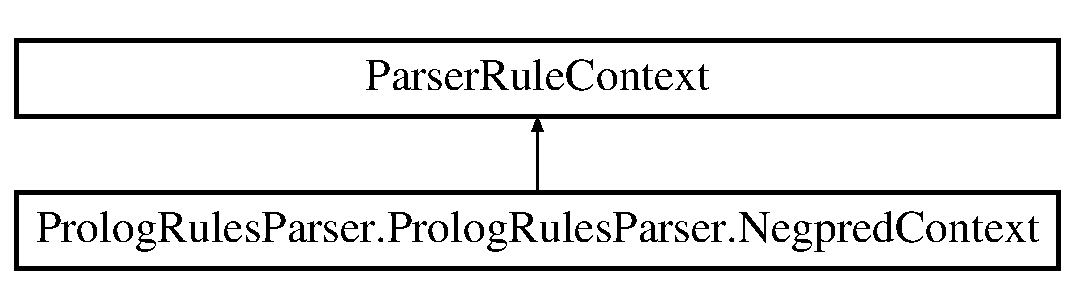
\includegraphics[height=2.000000cm]{class_prolog_rules_parser_1_1_prolog_rules_parser_1_1_negpred_context}
\end{center}
\end{figure}
\subsection*{Public Member Functions}
\begin{DoxyCompactItemize}
\item 
def \hyperlink{class_prolog_rules_parser_1_1_prolog_rules_parser_1_1_negpred_context_a40efc79fd3d05195cf11000bf135f2c3}{\+\_\+\+\_\+init\+\_\+\+\_\+}
\item 
def \hyperlink{class_prolog_rules_parser_1_1_prolog_rules_parser_1_1_negpred_context_a27d1ef33b96942ddcf08f1bee2d64094}{predicate} (self)
\item 
def \hyperlink{class_prolog_rules_parser_1_1_prolog_rules_parser_1_1_negpred_context_a005a7204a6f408bf3d123ccc1358ba0f}{get\+Rule\+Index} (self)
\item 
def \hyperlink{class_prolog_rules_parser_1_1_prolog_rules_parser_1_1_negpred_context_a549a9924eeb8f9a50df73bdfb21cf3f4}{enter\+Rule} (self, listener)
\item 
def \hyperlink{class_prolog_rules_parser_1_1_prolog_rules_parser_1_1_negpred_context_a1535ce17471bbc8929a322a7537bb866}{exit\+Rule} (self, listener)
\end{DoxyCompactItemize}
\subsection*{Public Attributes}
\begin{DoxyCompactItemize}
\item 
\hyperlink{class_prolog_rules_parser_1_1_prolog_rules_parser_1_1_negpred_context_a25d436043a2b3c31d38202d859a326b3}{parser}
\end{DoxyCompactItemize}


\subsection{Detailed Description}


Definition at line 811 of file Prolog\+Rules\+Parser.\+py.



\subsection{Constructor \& Destructor Documentation}
\hypertarget{class_prolog_rules_parser_1_1_prolog_rules_parser_1_1_negpred_context_a40efc79fd3d05195cf11000bf135f2c3}{}\index{Prolog\+Rules\+Parser\+::\+Prolog\+Rules\+Parser\+::\+Negpred\+Context@{Prolog\+Rules\+Parser\+::\+Prolog\+Rules\+Parser\+::\+Negpred\+Context}!\+\_\+\+\_\+init\+\_\+\+\_\+@{\+\_\+\+\_\+init\+\_\+\+\_\+}}
\index{\+\_\+\+\_\+init\+\_\+\+\_\+@{\+\_\+\+\_\+init\+\_\+\+\_\+}!Prolog\+Rules\+Parser\+::\+Prolog\+Rules\+Parser\+::\+Negpred\+Context@{Prolog\+Rules\+Parser\+::\+Prolog\+Rules\+Parser\+::\+Negpred\+Context}}
\subsubsection[{\+\_\+\+\_\+init\+\_\+\+\_\+}]{\setlength{\rightskip}{0pt plus 5cm}def Prolog\+Rules\+Parser.\+Prolog\+Rules\+Parser.\+Negpred\+Context.\+\_\+\+\_\+init\+\_\+\+\_\+ (
\begin{DoxyParamCaption}
\item[{}]{self, }
\item[{}]{parser, }
\item[{}]{parent = {\ttfamily None}, }
\item[{}]{invoking\+State = {\ttfamily -\/1}}
\end{DoxyParamCaption}
)}\label{class_prolog_rules_parser_1_1_prolog_rules_parser_1_1_negpred_context_a40efc79fd3d05195cf11000bf135f2c3}


Definition at line 813 of file Prolog\+Rules\+Parser.\+py.



\subsection{Member Function Documentation}
\hypertarget{class_prolog_rules_parser_1_1_prolog_rules_parser_1_1_negpred_context_a549a9924eeb8f9a50df73bdfb21cf3f4}{}\index{Prolog\+Rules\+Parser\+::\+Prolog\+Rules\+Parser\+::\+Negpred\+Context@{Prolog\+Rules\+Parser\+::\+Prolog\+Rules\+Parser\+::\+Negpred\+Context}!enter\+Rule@{enter\+Rule}}
\index{enter\+Rule@{enter\+Rule}!Prolog\+Rules\+Parser\+::\+Prolog\+Rules\+Parser\+::\+Negpred\+Context@{Prolog\+Rules\+Parser\+::\+Prolog\+Rules\+Parser\+::\+Negpred\+Context}}
\subsubsection[{enter\+Rule}]{\setlength{\rightskip}{0pt plus 5cm}def Prolog\+Rules\+Parser.\+Prolog\+Rules\+Parser.\+Negpred\+Context.\+enter\+Rule (
\begin{DoxyParamCaption}
\item[{}]{self, }
\item[{}]{listener}
\end{DoxyParamCaption}
)}\label{class_prolog_rules_parser_1_1_prolog_rules_parser_1_1_negpred_context_a549a9924eeb8f9a50df73bdfb21cf3f4}


Definition at line 824 of file Prolog\+Rules\+Parser.\+py.

\hypertarget{class_prolog_rules_parser_1_1_prolog_rules_parser_1_1_negpred_context_a1535ce17471bbc8929a322a7537bb866}{}\index{Prolog\+Rules\+Parser\+::\+Prolog\+Rules\+Parser\+::\+Negpred\+Context@{Prolog\+Rules\+Parser\+::\+Prolog\+Rules\+Parser\+::\+Negpred\+Context}!exit\+Rule@{exit\+Rule}}
\index{exit\+Rule@{exit\+Rule}!Prolog\+Rules\+Parser\+::\+Prolog\+Rules\+Parser\+::\+Negpred\+Context@{Prolog\+Rules\+Parser\+::\+Prolog\+Rules\+Parser\+::\+Negpred\+Context}}
\subsubsection[{exit\+Rule}]{\setlength{\rightskip}{0pt plus 5cm}def Prolog\+Rules\+Parser.\+Prolog\+Rules\+Parser.\+Negpred\+Context.\+exit\+Rule (
\begin{DoxyParamCaption}
\item[{}]{self, }
\item[{}]{listener}
\end{DoxyParamCaption}
)}\label{class_prolog_rules_parser_1_1_prolog_rules_parser_1_1_negpred_context_a1535ce17471bbc8929a322a7537bb866}


Definition at line 828 of file Prolog\+Rules\+Parser.\+py.

\hypertarget{class_prolog_rules_parser_1_1_prolog_rules_parser_1_1_negpred_context_a005a7204a6f408bf3d123ccc1358ba0f}{}\index{Prolog\+Rules\+Parser\+::\+Prolog\+Rules\+Parser\+::\+Negpred\+Context@{Prolog\+Rules\+Parser\+::\+Prolog\+Rules\+Parser\+::\+Negpred\+Context}!get\+Rule\+Index@{get\+Rule\+Index}}
\index{get\+Rule\+Index@{get\+Rule\+Index}!Prolog\+Rules\+Parser\+::\+Prolog\+Rules\+Parser\+::\+Negpred\+Context@{Prolog\+Rules\+Parser\+::\+Prolog\+Rules\+Parser\+::\+Negpred\+Context}}
\subsubsection[{get\+Rule\+Index}]{\setlength{\rightskip}{0pt plus 5cm}def Prolog\+Rules\+Parser.\+Prolog\+Rules\+Parser.\+Negpred\+Context.\+get\+Rule\+Index (
\begin{DoxyParamCaption}
\item[{}]{self}
\end{DoxyParamCaption}
)}\label{class_prolog_rules_parser_1_1_prolog_rules_parser_1_1_negpred_context_a005a7204a6f408bf3d123ccc1358ba0f}


Definition at line 821 of file Prolog\+Rules\+Parser.\+py.

\hypertarget{class_prolog_rules_parser_1_1_prolog_rules_parser_1_1_negpred_context_a27d1ef33b96942ddcf08f1bee2d64094}{}\index{Prolog\+Rules\+Parser\+::\+Prolog\+Rules\+Parser\+::\+Negpred\+Context@{Prolog\+Rules\+Parser\+::\+Prolog\+Rules\+Parser\+::\+Negpred\+Context}!predicate@{predicate}}
\index{predicate@{predicate}!Prolog\+Rules\+Parser\+::\+Prolog\+Rules\+Parser\+::\+Negpred\+Context@{Prolog\+Rules\+Parser\+::\+Prolog\+Rules\+Parser\+::\+Negpred\+Context}}
\subsubsection[{predicate}]{\setlength{\rightskip}{0pt plus 5cm}def Prolog\+Rules\+Parser.\+Prolog\+Rules\+Parser.\+Negpred\+Context.\+predicate (
\begin{DoxyParamCaption}
\item[{}]{self}
\end{DoxyParamCaption}
)}\label{class_prolog_rules_parser_1_1_prolog_rules_parser_1_1_negpred_context_a27d1ef33b96942ddcf08f1bee2d64094}


Definition at line 817 of file Prolog\+Rules\+Parser.\+py.



\subsection{Member Data Documentation}
\hypertarget{class_prolog_rules_parser_1_1_prolog_rules_parser_1_1_negpred_context_a25d436043a2b3c31d38202d859a326b3}{}\index{Prolog\+Rules\+Parser\+::\+Prolog\+Rules\+Parser\+::\+Negpred\+Context@{Prolog\+Rules\+Parser\+::\+Prolog\+Rules\+Parser\+::\+Negpred\+Context}!parser@{parser}}
\index{parser@{parser}!Prolog\+Rules\+Parser\+::\+Prolog\+Rules\+Parser\+::\+Negpred\+Context@{Prolog\+Rules\+Parser\+::\+Prolog\+Rules\+Parser\+::\+Negpred\+Context}}
\subsubsection[{parser}]{\setlength{\rightskip}{0pt plus 5cm}Prolog\+Rules\+Parser.\+Prolog\+Rules\+Parser.\+Negpred\+Context.\+parser}\label{class_prolog_rules_parser_1_1_prolog_rules_parser_1_1_negpred_context_a25d436043a2b3c31d38202d859a326b3}


Definition at line 815 of file Prolog\+Rules\+Parser.\+py.



The documentation for this class was generated from the following file\+:\begin{DoxyCompactItemize}
\item 
\hyperlink{_prolog_rules_parser_8py}{Prolog\+Rules\+Parser.\+py}\end{DoxyCompactItemize}

\hypertarget{class_prolog_rules_parser_1_1_prolog_rules_parser_1_1_onearg_context}{}\section{Prolog\+Rules\+Parser.\+Prolog\+Rules\+Parser.\+Onearg\+Context Class Reference}
\label{class_prolog_rules_parser_1_1_prolog_rules_parser_1_1_onearg_context}\index{Prolog\+Rules\+Parser.\+Prolog\+Rules\+Parser.\+Onearg\+Context@{Prolog\+Rules\+Parser.\+Prolog\+Rules\+Parser.\+Onearg\+Context}}
Inheritance diagram for Prolog\+Rules\+Parser.\+Prolog\+Rules\+Parser.\+Onearg\+Context\+:\begin{figure}[H]
\begin{center}
\leavevmode
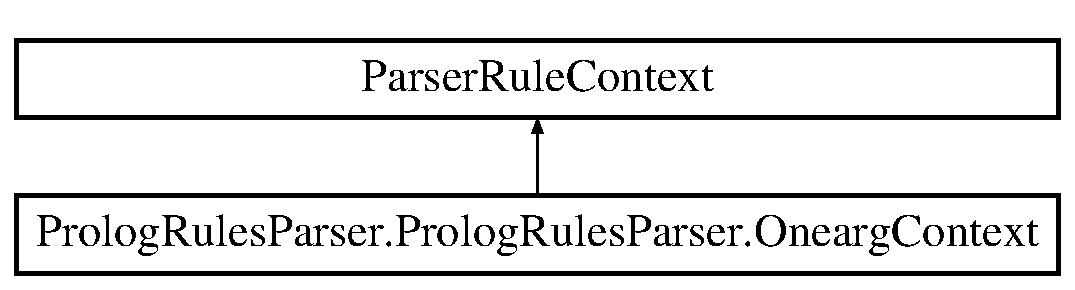
\includegraphics[height=2.000000cm]{class_prolog_rules_parser_1_1_prolog_rules_parser_1_1_onearg_context}
\end{center}
\end{figure}
\subsection*{Public Member Functions}
\begin{DoxyCompactItemize}
\item 
def \hyperlink{class_prolog_rules_parser_1_1_prolog_rules_parser_1_1_onearg_context_a3bc8833fba8dc822918de0d55fcc430a}{\+\_\+\+\_\+init\+\_\+\+\_\+}
\item 
def \hyperlink{class_prolog_rules_parser_1_1_prolog_rules_parser_1_1_onearg_context_a4e847f53fcbea7cc7e54db1f36300027}{predicate} (self)
\item 
def \hyperlink{class_prolog_rules_parser_1_1_prolog_rules_parser_1_1_onearg_context_a28bfd2a3d58241a8225eb2eec4820702}{atom} (self)
\item 
def \hyperlink{class_prolog_rules_parser_1_1_prolog_rules_parser_1_1_onearg_context_ad68a1ac517b420c88645fba6f77ab47b}{get\+Rule\+Index} (self)
\item 
def \hyperlink{class_prolog_rules_parser_1_1_prolog_rules_parser_1_1_onearg_context_ae5fb9dd2d757ca626f9e44d2fc67a9ab}{enter\+Rule} (self, listener)
\item 
def \hyperlink{class_prolog_rules_parser_1_1_prolog_rules_parser_1_1_onearg_context_a9eaa5290d5837af9efed07393e65407b}{exit\+Rule} (self, listener)
\end{DoxyCompactItemize}
\subsection*{Public Attributes}
\begin{DoxyCompactItemize}
\item 
\hyperlink{class_prolog_rules_parser_1_1_prolog_rules_parser_1_1_onearg_context_a04880e1b11723c07767be3f5cf97af82}{parser}
\end{DoxyCompactItemize}


\subsection{Detailed Description}


Definition at line 1041 of file Prolog\+Rules\+Parser.\+py.



\subsection{Constructor \& Destructor Documentation}
\hypertarget{class_prolog_rules_parser_1_1_prolog_rules_parser_1_1_onearg_context_a3bc8833fba8dc822918de0d55fcc430a}{}\index{Prolog\+Rules\+Parser\+::\+Prolog\+Rules\+Parser\+::\+Onearg\+Context@{Prolog\+Rules\+Parser\+::\+Prolog\+Rules\+Parser\+::\+Onearg\+Context}!\+\_\+\+\_\+init\+\_\+\+\_\+@{\+\_\+\+\_\+init\+\_\+\+\_\+}}
\index{\+\_\+\+\_\+init\+\_\+\+\_\+@{\+\_\+\+\_\+init\+\_\+\+\_\+}!Prolog\+Rules\+Parser\+::\+Prolog\+Rules\+Parser\+::\+Onearg\+Context@{Prolog\+Rules\+Parser\+::\+Prolog\+Rules\+Parser\+::\+Onearg\+Context}}
\subsubsection[{\+\_\+\+\_\+init\+\_\+\+\_\+}]{\setlength{\rightskip}{0pt plus 5cm}def Prolog\+Rules\+Parser.\+Prolog\+Rules\+Parser.\+Onearg\+Context.\+\_\+\+\_\+init\+\_\+\+\_\+ (
\begin{DoxyParamCaption}
\item[{}]{self, }
\item[{}]{parser, }
\item[{}]{parent = {\ttfamily None}, }
\item[{}]{invoking\+State = {\ttfamily -\/1}}
\end{DoxyParamCaption}
)}\label{class_prolog_rules_parser_1_1_prolog_rules_parser_1_1_onearg_context_a3bc8833fba8dc822918de0d55fcc430a}


Definition at line 1043 of file Prolog\+Rules\+Parser.\+py.



\subsection{Member Function Documentation}
\hypertarget{class_prolog_rules_parser_1_1_prolog_rules_parser_1_1_onearg_context_a28bfd2a3d58241a8225eb2eec4820702}{}\index{Prolog\+Rules\+Parser\+::\+Prolog\+Rules\+Parser\+::\+Onearg\+Context@{Prolog\+Rules\+Parser\+::\+Prolog\+Rules\+Parser\+::\+Onearg\+Context}!atom@{atom}}
\index{atom@{atom}!Prolog\+Rules\+Parser\+::\+Prolog\+Rules\+Parser\+::\+Onearg\+Context@{Prolog\+Rules\+Parser\+::\+Prolog\+Rules\+Parser\+::\+Onearg\+Context}}
\subsubsection[{atom}]{\setlength{\rightskip}{0pt plus 5cm}def Prolog\+Rules\+Parser.\+Prolog\+Rules\+Parser.\+Onearg\+Context.\+atom (
\begin{DoxyParamCaption}
\item[{}]{self}
\end{DoxyParamCaption}
)}\label{class_prolog_rules_parser_1_1_prolog_rules_parser_1_1_onearg_context_a28bfd2a3d58241a8225eb2eec4820702}


Definition at line 1051 of file Prolog\+Rules\+Parser.\+py.

\hypertarget{class_prolog_rules_parser_1_1_prolog_rules_parser_1_1_onearg_context_ae5fb9dd2d757ca626f9e44d2fc67a9ab}{}\index{Prolog\+Rules\+Parser\+::\+Prolog\+Rules\+Parser\+::\+Onearg\+Context@{Prolog\+Rules\+Parser\+::\+Prolog\+Rules\+Parser\+::\+Onearg\+Context}!enter\+Rule@{enter\+Rule}}
\index{enter\+Rule@{enter\+Rule}!Prolog\+Rules\+Parser\+::\+Prolog\+Rules\+Parser\+::\+Onearg\+Context@{Prolog\+Rules\+Parser\+::\+Prolog\+Rules\+Parser\+::\+Onearg\+Context}}
\subsubsection[{enter\+Rule}]{\setlength{\rightskip}{0pt plus 5cm}def Prolog\+Rules\+Parser.\+Prolog\+Rules\+Parser.\+Onearg\+Context.\+enter\+Rule (
\begin{DoxyParamCaption}
\item[{}]{self, }
\item[{}]{listener}
\end{DoxyParamCaption}
)}\label{class_prolog_rules_parser_1_1_prolog_rules_parser_1_1_onearg_context_ae5fb9dd2d757ca626f9e44d2fc67a9ab}


Definition at line 1058 of file Prolog\+Rules\+Parser.\+py.

\hypertarget{class_prolog_rules_parser_1_1_prolog_rules_parser_1_1_onearg_context_a9eaa5290d5837af9efed07393e65407b}{}\index{Prolog\+Rules\+Parser\+::\+Prolog\+Rules\+Parser\+::\+Onearg\+Context@{Prolog\+Rules\+Parser\+::\+Prolog\+Rules\+Parser\+::\+Onearg\+Context}!exit\+Rule@{exit\+Rule}}
\index{exit\+Rule@{exit\+Rule}!Prolog\+Rules\+Parser\+::\+Prolog\+Rules\+Parser\+::\+Onearg\+Context@{Prolog\+Rules\+Parser\+::\+Prolog\+Rules\+Parser\+::\+Onearg\+Context}}
\subsubsection[{exit\+Rule}]{\setlength{\rightskip}{0pt plus 5cm}def Prolog\+Rules\+Parser.\+Prolog\+Rules\+Parser.\+Onearg\+Context.\+exit\+Rule (
\begin{DoxyParamCaption}
\item[{}]{self, }
\item[{}]{listener}
\end{DoxyParamCaption}
)}\label{class_prolog_rules_parser_1_1_prolog_rules_parser_1_1_onearg_context_a9eaa5290d5837af9efed07393e65407b}


Definition at line 1062 of file Prolog\+Rules\+Parser.\+py.

\hypertarget{class_prolog_rules_parser_1_1_prolog_rules_parser_1_1_onearg_context_ad68a1ac517b420c88645fba6f77ab47b}{}\index{Prolog\+Rules\+Parser\+::\+Prolog\+Rules\+Parser\+::\+Onearg\+Context@{Prolog\+Rules\+Parser\+::\+Prolog\+Rules\+Parser\+::\+Onearg\+Context}!get\+Rule\+Index@{get\+Rule\+Index}}
\index{get\+Rule\+Index@{get\+Rule\+Index}!Prolog\+Rules\+Parser\+::\+Prolog\+Rules\+Parser\+::\+Onearg\+Context@{Prolog\+Rules\+Parser\+::\+Prolog\+Rules\+Parser\+::\+Onearg\+Context}}
\subsubsection[{get\+Rule\+Index}]{\setlength{\rightskip}{0pt plus 5cm}def Prolog\+Rules\+Parser.\+Prolog\+Rules\+Parser.\+Onearg\+Context.\+get\+Rule\+Index (
\begin{DoxyParamCaption}
\item[{}]{self}
\end{DoxyParamCaption}
)}\label{class_prolog_rules_parser_1_1_prolog_rules_parser_1_1_onearg_context_ad68a1ac517b420c88645fba6f77ab47b}


Definition at line 1055 of file Prolog\+Rules\+Parser.\+py.

\hypertarget{class_prolog_rules_parser_1_1_prolog_rules_parser_1_1_onearg_context_a4e847f53fcbea7cc7e54db1f36300027}{}\index{Prolog\+Rules\+Parser\+::\+Prolog\+Rules\+Parser\+::\+Onearg\+Context@{Prolog\+Rules\+Parser\+::\+Prolog\+Rules\+Parser\+::\+Onearg\+Context}!predicate@{predicate}}
\index{predicate@{predicate}!Prolog\+Rules\+Parser\+::\+Prolog\+Rules\+Parser\+::\+Onearg\+Context@{Prolog\+Rules\+Parser\+::\+Prolog\+Rules\+Parser\+::\+Onearg\+Context}}
\subsubsection[{predicate}]{\setlength{\rightskip}{0pt plus 5cm}def Prolog\+Rules\+Parser.\+Prolog\+Rules\+Parser.\+Onearg\+Context.\+predicate (
\begin{DoxyParamCaption}
\item[{}]{self}
\end{DoxyParamCaption}
)}\label{class_prolog_rules_parser_1_1_prolog_rules_parser_1_1_onearg_context_a4e847f53fcbea7cc7e54db1f36300027}


Definition at line 1047 of file Prolog\+Rules\+Parser.\+py.



\subsection{Member Data Documentation}
\hypertarget{class_prolog_rules_parser_1_1_prolog_rules_parser_1_1_onearg_context_a04880e1b11723c07767be3f5cf97af82}{}\index{Prolog\+Rules\+Parser\+::\+Prolog\+Rules\+Parser\+::\+Onearg\+Context@{Prolog\+Rules\+Parser\+::\+Prolog\+Rules\+Parser\+::\+Onearg\+Context}!parser@{parser}}
\index{parser@{parser}!Prolog\+Rules\+Parser\+::\+Prolog\+Rules\+Parser\+::\+Onearg\+Context@{Prolog\+Rules\+Parser\+::\+Prolog\+Rules\+Parser\+::\+Onearg\+Context}}
\subsubsection[{parser}]{\setlength{\rightskip}{0pt plus 5cm}Prolog\+Rules\+Parser.\+Prolog\+Rules\+Parser.\+Onearg\+Context.\+parser}\label{class_prolog_rules_parser_1_1_prolog_rules_parser_1_1_onearg_context_a04880e1b11723c07767be3f5cf97af82}


Definition at line 1045 of file Prolog\+Rules\+Parser.\+py.



The documentation for this class was generated from the following file\+:\begin{DoxyCompactItemize}
\item 
\hyperlink{_prolog_rules_parser_8py}{Prolog\+Rules\+Parser.\+py}\end{DoxyCompactItemize}

\hypertarget{class_prolog_rules_parser_1_1_prolog_rules_parser_1_1_predcount_context}{}\section{Prolog\+Rules\+Parser.\+Prolog\+Rules\+Parser.\+Predcount\+Context Class Reference}
\label{class_prolog_rules_parser_1_1_prolog_rules_parser_1_1_predcount_context}\index{Prolog\+Rules\+Parser.\+Prolog\+Rules\+Parser.\+Predcount\+Context@{Prolog\+Rules\+Parser.\+Prolog\+Rules\+Parser.\+Predcount\+Context}}
Inheritance diagram for Prolog\+Rules\+Parser.\+Prolog\+Rules\+Parser.\+Predcount\+Context\+:\begin{figure}[H]
\begin{center}
\leavevmode
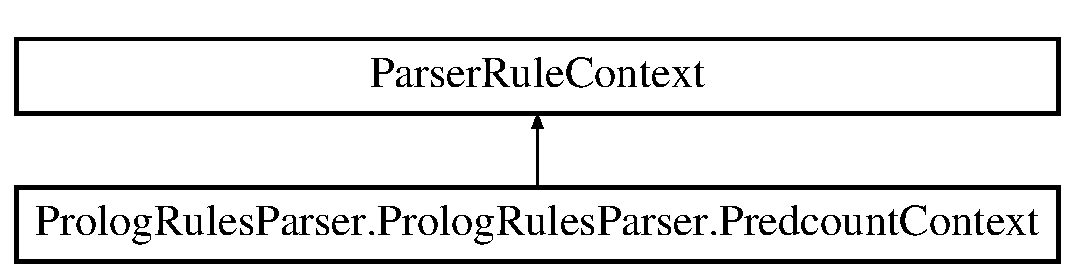
\includegraphics[height=2.000000cm]{class_prolog_rules_parser_1_1_prolog_rules_parser_1_1_predcount_context}
\end{center}
\end{figure}
\subsection*{Public Member Functions}
\begin{DoxyCompactItemize}
\item 
def \hyperlink{class_prolog_rules_parser_1_1_prolog_rules_parser_1_1_predcount_context_a7837e1358659bfab6eb373b92d38a815}{\+\_\+\+\_\+init\+\_\+\+\_\+}
\item 
def \hyperlink{class_prolog_rules_parser_1_1_prolog_rules_parser_1_1_predcount_context_a0df38c740797c548a46652426b8824e1}{atom}
\item 
def \hyperlink{class_prolog_rules_parser_1_1_prolog_rules_parser_1_1_predcount_context_a54de76dfff1fe7e9f35b891832cf1771}{rulebody} (self)
\item 
def \hyperlink{class_prolog_rules_parser_1_1_prolog_rules_parser_1_1_predcount_context_ace356a956b3027bfb9a004ee047784c2}{predicate} (self)
\item 
def \hyperlink{class_prolog_rules_parser_1_1_prolog_rules_parser_1_1_predcount_context_a8ee46d759d408258c5b4813432f75725}{get\+Rule\+Index} (self)
\item 
def \hyperlink{class_prolog_rules_parser_1_1_prolog_rules_parser_1_1_predcount_context_a5a0060e6e8675c5aff674842485507f7}{enter\+Rule} (self, listener)
\item 
def \hyperlink{class_prolog_rules_parser_1_1_prolog_rules_parser_1_1_predcount_context_a06a84b0c80e4ac350a4d176c70a446e2}{exit\+Rule} (self, listener)
\end{DoxyCompactItemize}
\subsection*{Public Attributes}
\begin{DoxyCompactItemize}
\item 
\hyperlink{class_prolog_rules_parser_1_1_prolog_rules_parser_1_1_predcount_context_a265082cf0109e603962e8fe6d2b1904f}{parser}
\end{DoxyCompactItemize}


\subsection{Detailed Description}


Definition at line 534 of file Prolog\+Rules\+Parser.\+py.



\subsection{Constructor \& Destructor Documentation}
\hypertarget{class_prolog_rules_parser_1_1_prolog_rules_parser_1_1_predcount_context_a7837e1358659bfab6eb373b92d38a815}{}\index{Prolog\+Rules\+Parser\+::\+Prolog\+Rules\+Parser\+::\+Predcount\+Context@{Prolog\+Rules\+Parser\+::\+Prolog\+Rules\+Parser\+::\+Predcount\+Context}!\+\_\+\+\_\+init\+\_\+\+\_\+@{\+\_\+\+\_\+init\+\_\+\+\_\+}}
\index{\+\_\+\+\_\+init\+\_\+\+\_\+@{\+\_\+\+\_\+init\+\_\+\+\_\+}!Prolog\+Rules\+Parser\+::\+Prolog\+Rules\+Parser\+::\+Predcount\+Context@{Prolog\+Rules\+Parser\+::\+Prolog\+Rules\+Parser\+::\+Predcount\+Context}}
\subsubsection[{\+\_\+\+\_\+init\+\_\+\+\_\+}]{\setlength{\rightskip}{0pt plus 5cm}def Prolog\+Rules\+Parser.\+Prolog\+Rules\+Parser.\+Predcount\+Context.\+\_\+\+\_\+init\+\_\+\+\_\+ (
\begin{DoxyParamCaption}
\item[{}]{self, }
\item[{}]{parser, }
\item[{}]{parent = {\ttfamily None}, }
\item[{}]{invoking\+State = {\ttfamily -\/1}}
\end{DoxyParamCaption}
)}\label{class_prolog_rules_parser_1_1_prolog_rules_parser_1_1_predcount_context_a7837e1358659bfab6eb373b92d38a815}


Definition at line 536 of file Prolog\+Rules\+Parser.\+py.



\subsection{Member Function Documentation}
\hypertarget{class_prolog_rules_parser_1_1_prolog_rules_parser_1_1_predcount_context_a0df38c740797c548a46652426b8824e1}{}\index{Prolog\+Rules\+Parser\+::\+Prolog\+Rules\+Parser\+::\+Predcount\+Context@{Prolog\+Rules\+Parser\+::\+Prolog\+Rules\+Parser\+::\+Predcount\+Context}!atom@{atom}}
\index{atom@{atom}!Prolog\+Rules\+Parser\+::\+Prolog\+Rules\+Parser\+::\+Predcount\+Context@{Prolog\+Rules\+Parser\+::\+Prolog\+Rules\+Parser\+::\+Predcount\+Context}}
\subsubsection[{atom}]{\setlength{\rightskip}{0pt plus 5cm}def Prolog\+Rules\+Parser.\+Prolog\+Rules\+Parser.\+Predcount\+Context.\+atom (
\begin{DoxyParamCaption}
\item[{}]{self, }
\item[{}]{i = {\ttfamily None}}
\end{DoxyParamCaption}
)}\label{class_prolog_rules_parser_1_1_prolog_rules_parser_1_1_predcount_context_a0df38c740797c548a46652426b8824e1}


Definition at line 540 of file Prolog\+Rules\+Parser.\+py.

\hypertarget{class_prolog_rules_parser_1_1_prolog_rules_parser_1_1_predcount_context_a5a0060e6e8675c5aff674842485507f7}{}\index{Prolog\+Rules\+Parser\+::\+Prolog\+Rules\+Parser\+::\+Predcount\+Context@{Prolog\+Rules\+Parser\+::\+Prolog\+Rules\+Parser\+::\+Predcount\+Context}!enter\+Rule@{enter\+Rule}}
\index{enter\+Rule@{enter\+Rule}!Prolog\+Rules\+Parser\+::\+Prolog\+Rules\+Parser\+::\+Predcount\+Context@{Prolog\+Rules\+Parser\+::\+Prolog\+Rules\+Parser\+::\+Predcount\+Context}}
\subsubsection[{enter\+Rule}]{\setlength{\rightskip}{0pt plus 5cm}def Prolog\+Rules\+Parser.\+Prolog\+Rules\+Parser.\+Predcount\+Context.\+enter\+Rule (
\begin{DoxyParamCaption}
\item[{}]{self, }
\item[{}]{listener}
\end{DoxyParamCaption}
)}\label{class_prolog_rules_parser_1_1_prolog_rules_parser_1_1_predcount_context_a5a0060e6e8675c5aff674842485507f7}


Definition at line 558 of file Prolog\+Rules\+Parser.\+py.

\hypertarget{class_prolog_rules_parser_1_1_prolog_rules_parser_1_1_predcount_context_a06a84b0c80e4ac350a4d176c70a446e2}{}\index{Prolog\+Rules\+Parser\+::\+Prolog\+Rules\+Parser\+::\+Predcount\+Context@{Prolog\+Rules\+Parser\+::\+Prolog\+Rules\+Parser\+::\+Predcount\+Context}!exit\+Rule@{exit\+Rule}}
\index{exit\+Rule@{exit\+Rule}!Prolog\+Rules\+Parser\+::\+Prolog\+Rules\+Parser\+::\+Predcount\+Context@{Prolog\+Rules\+Parser\+::\+Prolog\+Rules\+Parser\+::\+Predcount\+Context}}
\subsubsection[{exit\+Rule}]{\setlength{\rightskip}{0pt plus 5cm}def Prolog\+Rules\+Parser.\+Prolog\+Rules\+Parser.\+Predcount\+Context.\+exit\+Rule (
\begin{DoxyParamCaption}
\item[{}]{self, }
\item[{}]{listener}
\end{DoxyParamCaption}
)}\label{class_prolog_rules_parser_1_1_prolog_rules_parser_1_1_predcount_context_a06a84b0c80e4ac350a4d176c70a446e2}


Definition at line 562 of file Prolog\+Rules\+Parser.\+py.

\hypertarget{class_prolog_rules_parser_1_1_prolog_rules_parser_1_1_predcount_context_a8ee46d759d408258c5b4813432f75725}{}\index{Prolog\+Rules\+Parser\+::\+Prolog\+Rules\+Parser\+::\+Predcount\+Context@{Prolog\+Rules\+Parser\+::\+Prolog\+Rules\+Parser\+::\+Predcount\+Context}!get\+Rule\+Index@{get\+Rule\+Index}}
\index{get\+Rule\+Index@{get\+Rule\+Index}!Prolog\+Rules\+Parser\+::\+Prolog\+Rules\+Parser\+::\+Predcount\+Context@{Prolog\+Rules\+Parser\+::\+Prolog\+Rules\+Parser\+::\+Predcount\+Context}}
\subsubsection[{get\+Rule\+Index}]{\setlength{\rightskip}{0pt plus 5cm}def Prolog\+Rules\+Parser.\+Prolog\+Rules\+Parser.\+Predcount\+Context.\+get\+Rule\+Index (
\begin{DoxyParamCaption}
\item[{}]{self}
\end{DoxyParamCaption}
)}\label{class_prolog_rules_parser_1_1_prolog_rules_parser_1_1_predcount_context_a8ee46d759d408258c5b4813432f75725}


Definition at line 555 of file Prolog\+Rules\+Parser.\+py.

\hypertarget{class_prolog_rules_parser_1_1_prolog_rules_parser_1_1_predcount_context_ace356a956b3027bfb9a004ee047784c2}{}\index{Prolog\+Rules\+Parser\+::\+Prolog\+Rules\+Parser\+::\+Predcount\+Context@{Prolog\+Rules\+Parser\+::\+Prolog\+Rules\+Parser\+::\+Predcount\+Context}!predicate@{predicate}}
\index{predicate@{predicate}!Prolog\+Rules\+Parser\+::\+Prolog\+Rules\+Parser\+::\+Predcount\+Context@{Prolog\+Rules\+Parser\+::\+Prolog\+Rules\+Parser\+::\+Predcount\+Context}}
\subsubsection[{predicate}]{\setlength{\rightskip}{0pt plus 5cm}def Prolog\+Rules\+Parser.\+Prolog\+Rules\+Parser.\+Predcount\+Context.\+predicate (
\begin{DoxyParamCaption}
\item[{}]{self}
\end{DoxyParamCaption}
)}\label{class_prolog_rules_parser_1_1_prolog_rules_parser_1_1_predcount_context_ace356a956b3027bfb9a004ee047784c2}


Definition at line 551 of file Prolog\+Rules\+Parser.\+py.

\hypertarget{class_prolog_rules_parser_1_1_prolog_rules_parser_1_1_predcount_context_a54de76dfff1fe7e9f35b891832cf1771}{}\index{Prolog\+Rules\+Parser\+::\+Prolog\+Rules\+Parser\+::\+Predcount\+Context@{Prolog\+Rules\+Parser\+::\+Prolog\+Rules\+Parser\+::\+Predcount\+Context}!rulebody@{rulebody}}
\index{rulebody@{rulebody}!Prolog\+Rules\+Parser\+::\+Prolog\+Rules\+Parser\+::\+Predcount\+Context@{Prolog\+Rules\+Parser\+::\+Prolog\+Rules\+Parser\+::\+Predcount\+Context}}
\subsubsection[{rulebody}]{\setlength{\rightskip}{0pt plus 5cm}def Prolog\+Rules\+Parser.\+Prolog\+Rules\+Parser.\+Predcount\+Context.\+rulebody (
\begin{DoxyParamCaption}
\item[{}]{self}
\end{DoxyParamCaption}
)}\label{class_prolog_rules_parser_1_1_prolog_rules_parser_1_1_predcount_context_a54de76dfff1fe7e9f35b891832cf1771}


Definition at line 547 of file Prolog\+Rules\+Parser.\+py.



\subsection{Member Data Documentation}
\hypertarget{class_prolog_rules_parser_1_1_prolog_rules_parser_1_1_predcount_context_a265082cf0109e603962e8fe6d2b1904f}{}\index{Prolog\+Rules\+Parser\+::\+Prolog\+Rules\+Parser\+::\+Predcount\+Context@{Prolog\+Rules\+Parser\+::\+Prolog\+Rules\+Parser\+::\+Predcount\+Context}!parser@{parser}}
\index{parser@{parser}!Prolog\+Rules\+Parser\+::\+Prolog\+Rules\+Parser\+::\+Predcount\+Context@{Prolog\+Rules\+Parser\+::\+Prolog\+Rules\+Parser\+::\+Predcount\+Context}}
\subsubsection[{parser}]{\setlength{\rightskip}{0pt plus 5cm}Prolog\+Rules\+Parser.\+Prolog\+Rules\+Parser.\+Predcount\+Context.\+parser}\label{class_prolog_rules_parser_1_1_prolog_rules_parser_1_1_predcount_context_a265082cf0109e603962e8fe6d2b1904f}


Definition at line 538 of file Prolog\+Rules\+Parser.\+py.



The documentation for this class was generated from the following file\+:\begin{DoxyCompactItemize}
\item 
\hyperlink{_prolog_rules_parser_8py}{Prolog\+Rules\+Parser.\+py}\end{DoxyCompactItemize}

\hypertarget{class_prolog_rules_parser_1_1_prolog_rules_parser_1_1_predicate_context}{}\section{Prolog\+Rules\+Parser.\+Prolog\+Rules\+Parser.\+Predicate\+Context Class Reference}
\label{class_prolog_rules_parser_1_1_prolog_rules_parser_1_1_predicate_context}\index{Prolog\+Rules\+Parser.\+Prolog\+Rules\+Parser.\+Predicate\+Context@{Prolog\+Rules\+Parser.\+Prolog\+Rules\+Parser.\+Predicate\+Context}}
Inheritance diagram for Prolog\+Rules\+Parser.\+Prolog\+Rules\+Parser.\+Predicate\+Context\+:\begin{figure}[H]
\begin{center}
\leavevmode
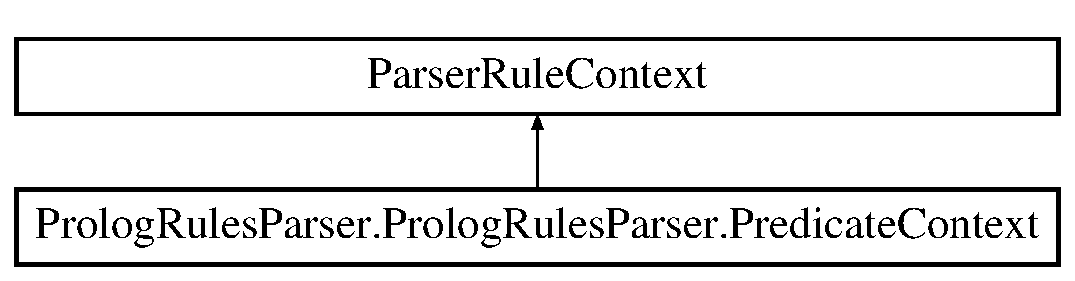
\includegraphics[height=2.000000cm]{class_prolog_rules_parser_1_1_prolog_rules_parser_1_1_predicate_context}
\end{center}
\end{figure}
\subsection*{Public Member Functions}
\begin{DoxyCompactItemize}
\item 
def \hyperlink{class_prolog_rules_parser_1_1_prolog_rules_parser_1_1_predicate_context_aa48fa3461c699520ceb02fc3faaae299}{\+\_\+\+\_\+init\+\_\+\+\_\+}
\item 
def \hyperlink{class_prolog_rules_parser_1_1_prolog_rules_parser_1_1_predicate_context_a1bae8b296f983c87c8cb5e5fc068be0f}{args} (self)
\item 
def \hyperlink{class_prolog_rules_parser_1_1_prolog_rules_parser_1_1_predicate_context_abd2fe75241cd23061984ace6734dc365}{identifier} (self)
\item 
def \hyperlink{class_prolog_rules_parser_1_1_prolog_rules_parser_1_1_predicate_context_ae7f34c611fba109e6f7eb8a4b987a3bc}{get\+Rule\+Index} (self)
\item 
def \hyperlink{class_prolog_rules_parser_1_1_prolog_rules_parser_1_1_predicate_context_a484ce1be14b5a667964a1658a7ac85ef}{enter\+Rule} (self, listener)
\item 
def \hyperlink{class_prolog_rules_parser_1_1_prolog_rules_parser_1_1_predicate_context_a3a4938688db551965ec17f47b9ba6f0a}{exit\+Rule} (self, listener)
\end{DoxyCompactItemize}
\subsection*{Public Attributes}
\begin{DoxyCompactItemize}
\item 
\hyperlink{class_prolog_rules_parser_1_1_prolog_rules_parser_1_1_predicate_context_addd1a629d2d7bde0d0a45bb3afce0432}{parser}
\end{DoxyCompactItemize}


\subsection{Detailed Description}


Definition at line 613 of file Prolog\+Rules\+Parser.\+py.



\subsection{Constructor \& Destructor Documentation}
\hypertarget{class_prolog_rules_parser_1_1_prolog_rules_parser_1_1_predicate_context_aa48fa3461c699520ceb02fc3faaae299}{}\index{Prolog\+Rules\+Parser\+::\+Prolog\+Rules\+Parser\+::\+Predicate\+Context@{Prolog\+Rules\+Parser\+::\+Prolog\+Rules\+Parser\+::\+Predicate\+Context}!\+\_\+\+\_\+init\+\_\+\+\_\+@{\+\_\+\+\_\+init\+\_\+\+\_\+}}
\index{\+\_\+\+\_\+init\+\_\+\+\_\+@{\+\_\+\+\_\+init\+\_\+\+\_\+}!Prolog\+Rules\+Parser\+::\+Prolog\+Rules\+Parser\+::\+Predicate\+Context@{Prolog\+Rules\+Parser\+::\+Prolog\+Rules\+Parser\+::\+Predicate\+Context}}
\subsubsection[{\+\_\+\+\_\+init\+\_\+\+\_\+}]{\setlength{\rightskip}{0pt plus 5cm}def Prolog\+Rules\+Parser.\+Prolog\+Rules\+Parser.\+Predicate\+Context.\+\_\+\+\_\+init\+\_\+\+\_\+ (
\begin{DoxyParamCaption}
\item[{}]{self, }
\item[{}]{parser, }
\item[{}]{parent = {\ttfamily None}, }
\item[{}]{invoking\+State = {\ttfamily -\/1}}
\end{DoxyParamCaption}
)}\label{class_prolog_rules_parser_1_1_prolog_rules_parser_1_1_predicate_context_aa48fa3461c699520ceb02fc3faaae299}


Definition at line 615 of file Prolog\+Rules\+Parser.\+py.



\subsection{Member Function Documentation}
\hypertarget{class_prolog_rules_parser_1_1_prolog_rules_parser_1_1_predicate_context_a1bae8b296f983c87c8cb5e5fc068be0f}{}\index{Prolog\+Rules\+Parser\+::\+Prolog\+Rules\+Parser\+::\+Predicate\+Context@{Prolog\+Rules\+Parser\+::\+Prolog\+Rules\+Parser\+::\+Predicate\+Context}!args@{args}}
\index{args@{args}!Prolog\+Rules\+Parser\+::\+Prolog\+Rules\+Parser\+::\+Predicate\+Context@{Prolog\+Rules\+Parser\+::\+Prolog\+Rules\+Parser\+::\+Predicate\+Context}}
\subsubsection[{args}]{\setlength{\rightskip}{0pt plus 5cm}def Prolog\+Rules\+Parser.\+Prolog\+Rules\+Parser.\+Predicate\+Context.\+args (
\begin{DoxyParamCaption}
\item[{}]{self}
\end{DoxyParamCaption}
)}\label{class_prolog_rules_parser_1_1_prolog_rules_parser_1_1_predicate_context_a1bae8b296f983c87c8cb5e5fc068be0f}


Definition at line 619 of file Prolog\+Rules\+Parser.\+py.

\hypertarget{class_prolog_rules_parser_1_1_prolog_rules_parser_1_1_predicate_context_a484ce1be14b5a667964a1658a7ac85ef}{}\index{Prolog\+Rules\+Parser\+::\+Prolog\+Rules\+Parser\+::\+Predicate\+Context@{Prolog\+Rules\+Parser\+::\+Prolog\+Rules\+Parser\+::\+Predicate\+Context}!enter\+Rule@{enter\+Rule}}
\index{enter\+Rule@{enter\+Rule}!Prolog\+Rules\+Parser\+::\+Prolog\+Rules\+Parser\+::\+Predicate\+Context@{Prolog\+Rules\+Parser\+::\+Prolog\+Rules\+Parser\+::\+Predicate\+Context}}
\subsubsection[{enter\+Rule}]{\setlength{\rightskip}{0pt plus 5cm}def Prolog\+Rules\+Parser.\+Prolog\+Rules\+Parser.\+Predicate\+Context.\+enter\+Rule (
\begin{DoxyParamCaption}
\item[{}]{self, }
\item[{}]{listener}
\end{DoxyParamCaption}
)}\label{class_prolog_rules_parser_1_1_prolog_rules_parser_1_1_predicate_context_a484ce1be14b5a667964a1658a7ac85ef}


Definition at line 630 of file Prolog\+Rules\+Parser.\+py.

\hypertarget{class_prolog_rules_parser_1_1_prolog_rules_parser_1_1_predicate_context_a3a4938688db551965ec17f47b9ba6f0a}{}\index{Prolog\+Rules\+Parser\+::\+Prolog\+Rules\+Parser\+::\+Predicate\+Context@{Prolog\+Rules\+Parser\+::\+Prolog\+Rules\+Parser\+::\+Predicate\+Context}!exit\+Rule@{exit\+Rule}}
\index{exit\+Rule@{exit\+Rule}!Prolog\+Rules\+Parser\+::\+Prolog\+Rules\+Parser\+::\+Predicate\+Context@{Prolog\+Rules\+Parser\+::\+Prolog\+Rules\+Parser\+::\+Predicate\+Context}}
\subsubsection[{exit\+Rule}]{\setlength{\rightskip}{0pt plus 5cm}def Prolog\+Rules\+Parser.\+Prolog\+Rules\+Parser.\+Predicate\+Context.\+exit\+Rule (
\begin{DoxyParamCaption}
\item[{}]{self, }
\item[{}]{listener}
\end{DoxyParamCaption}
)}\label{class_prolog_rules_parser_1_1_prolog_rules_parser_1_1_predicate_context_a3a4938688db551965ec17f47b9ba6f0a}


Definition at line 634 of file Prolog\+Rules\+Parser.\+py.

\hypertarget{class_prolog_rules_parser_1_1_prolog_rules_parser_1_1_predicate_context_ae7f34c611fba109e6f7eb8a4b987a3bc}{}\index{Prolog\+Rules\+Parser\+::\+Prolog\+Rules\+Parser\+::\+Predicate\+Context@{Prolog\+Rules\+Parser\+::\+Prolog\+Rules\+Parser\+::\+Predicate\+Context}!get\+Rule\+Index@{get\+Rule\+Index}}
\index{get\+Rule\+Index@{get\+Rule\+Index}!Prolog\+Rules\+Parser\+::\+Prolog\+Rules\+Parser\+::\+Predicate\+Context@{Prolog\+Rules\+Parser\+::\+Prolog\+Rules\+Parser\+::\+Predicate\+Context}}
\subsubsection[{get\+Rule\+Index}]{\setlength{\rightskip}{0pt plus 5cm}def Prolog\+Rules\+Parser.\+Prolog\+Rules\+Parser.\+Predicate\+Context.\+get\+Rule\+Index (
\begin{DoxyParamCaption}
\item[{}]{self}
\end{DoxyParamCaption}
)}\label{class_prolog_rules_parser_1_1_prolog_rules_parser_1_1_predicate_context_ae7f34c611fba109e6f7eb8a4b987a3bc}


Definition at line 627 of file Prolog\+Rules\+Parser.\+py.

\hypertarget{class_prolog_rules_parser_1_1_prolog_rules_parser_1_1_predicate_context_abd2fe75241cd23061984ace6734dc365}{}\index{Prolog\+Rules\+Parser\+::\+Prolog\+Rules\+Parser\+::\+Predicate\+Context@{Prolog\+Rules\+Parser\+::\+Prolog\+Rules\+Parser\+::\+Predicate\+Context}!identifier@{identifier}}
\index{identifier@{identifier}!Prolog\+Rules\+Parser\+::\+Prolog\+Rules\+Parser\+::\+Predicate\+Context@{Prolog\+Rules\+Parser\+::\+Prolog\+Rules\+Parser\+::\+Predicate\+Context}}
\subsubsection[{identifier}]{\setlength{\rightskip}{0pt plus 5cm}def Prolog\+Rules\+Parser.\+Prolog\+Rules\+Parser.\+Predicate\+Context.\+identifier (
\begin{DoxyParamCaption}
\item[{}]{self}
\end{DoxyParamCaption}
)}\label{class_prolog_rules_parser_1_1_prolog_rules_parser_1_1_predicate_context_abd2fe75241cd23061984ace6734dc365}


Definition at line 623 of file Prolog\+Rules\+Parser.\+py.



\subsection{Member Data Documentation}
\hypertarget{class_prolog_rules_parser_1_1_prolog_rules_parser_1_1_predicate_context_addd1a629d2d7bde0d0a45bb3afce0432}{}\index{Prolog\+Rules\+Parser\+::\+Prolog\+Rules\+Parser\+::\+Predicate\+Context@{Prolog\+Rules\+Parser\+::\+Prolog\+Rules\+Parser\+::\+Predicate\+Context}!parser@{parser}}
\index{parser@{parser}!Prolog\+Rules\+Parser\+::\+Prolog\+Rules\+Parser\+::\+Predicate\+Context@{Prolog\+Rules\+Parser\+::\+Prolog\+Rules\+Parser\+::\+Predicate\+Context}}
\subsubsection[{parser}]{\setlength{\rightskip}{0pt plus 5cm}Prolog\+Rules\+Parser.\+Prolog\+Rules\+Parser.\+Predicate\+Context.\+parser}\label{class_prolog_rules_parser_1_1_prolog_rules_parser_1_1_predicate_context_addd1a629d2d7bde0d0a45bb3afce0432}


Definition at line 617 of file Prolog\+Rules\+Parser.\+py.



The documentation for this class was generated from the following file\+:\begin{DoxyCompactItemize}
\item 
\hyperlink{_prolog_rules_parser_8py}{Prolog\+Rules\+Parser.\+py}\end{DoxyCompactItemize}

\hypertarget{classtotally__new__visualizer_1_1_problem_parser}{}\section{totally\+\_\+new\+\_\+visualizer.\+Problem\+Parser Class Reference}
\label{classtotally__new__visualizer_1_1_problem_parser}\index{totally\+\_\+new\+\_\+visualizer.\+Problem\+Parser@{totally\+\_\+new\+\_\+visualizer.\+Problem\+Parser}}


Handles the parsing of a single generated problem.  


Inheritance diagram for totally\+\_\+new\+\_\+visualizer.\+Problem\+Parser\+:\begin{figure}[H]
\begin{center}
\leavevmode
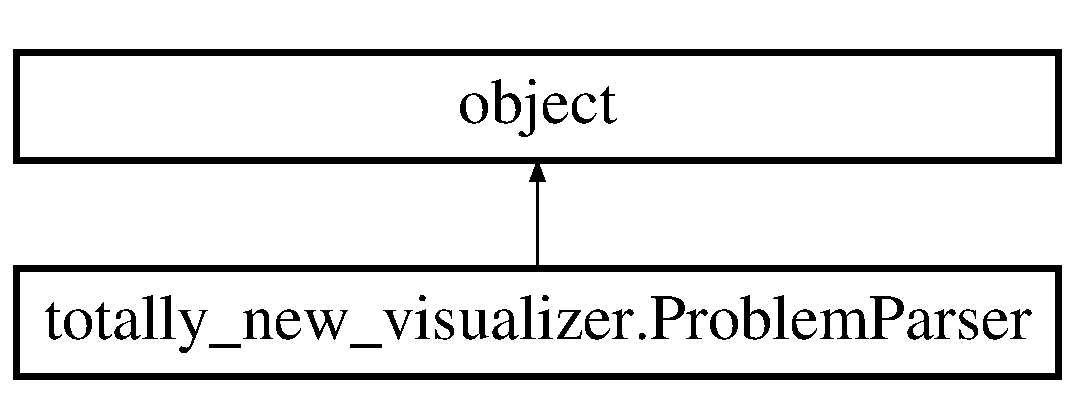
\includegraphics[height=2.000000cm]{classtotally__new__visualizer_1_1_problem_parser}
\end{center}
\end{figure}
\subsection*{Public Member Functions}
\begin{DoxyCompactItemize}
\item 
def \hyperlink{classtotally__new__visualizer_1_1_problem_parser_a8c74392fb4a04b5c3215fa594c1a223d}{\+\_\+\+\_\+init\+\_\+\+\_\+} (self, answer\+\_\+set\+\_\+predicates)
\item 
def \hyperlink{classtotally__new__visualizer_1_1_problem_parser_ada04c87da73191c9d9dd21f4bc7adbb9}{to\+Generated\+Solution} (self)
\begin{DoxyCompactList}\small\item\em \hyperlink{classtotally__new__visualizer_1_1_equation_step_parser}{Equation\+Step\+Parser} contains lots of data we don\textquotesingle{}t need after parsing this method returns a Generated\+Step instance that has only what we want to save. \end{DoxyCompactList}\item 
def \hyperlink{classtotally__new__visualizer_1_1_problem_parser_a3c480d50bf72818a2db48543b431bcbc}{add\+Predicate\+For\+Time\+Step} (self, time, pred\+\_\+obj)
\item 
def \hyperlink{classtotally__new__visualizer_1_1_problem_parser_a9ebe340d4c51febfe4b32a167d97e353}{parse\+Ans\+Set\+From\+Predicates} (self, predicates\+\_\+list)
\begin{DoxyCompactList}\small\item\em parse the given predicates into the steps the describe \end{DoxyCompactList}\item 
def \hyperlink{classtotally__new__visualizer_1_1_problem_parser_ae641da32655919b48a93bb263a565157}{solution\+Level\+Post\+Processing} (self)
\begin{DoxyCompactList}\small\item\em After all predicates are parsed, see if any post-\/processing needs to be done. \end{DoxyCompactList}\item 
def \hyperlink{classtotally__new__visualizer_1_1_problem_parser_aac1f2db24f810523852a67dbb69bfe5f}{get\+X\+Soln\+If\+Substitution\+Occurs} (self)
\begin{DoxyCompactList}\small\item\em Add soulutions for x if y-\/substitution is used; solver only solves for y if y substitution is used. \end{DoxyCompactList}\item 
def \hyperlink{classtotally__new__visualizer_1_1_problem_parser_afcfb1a63e8fe352e8e9a2737ea1654f5}{update\+Variables\+If\+Substitution\+Occurs} (self)
\begin{DoxyCompactList}\small\item\em if y-\/substitution is used, update the variable used for each step after the substitution \end{DoxyCompactList}\item 
def \hyperlink{classtotally__new__visualizer_1_1_problem_parser_a922001a638e085fc2ab3e08254eb60de}{get\+Solution\+String}
\begin{DoxyCompactList}\small\item\em T\+O\+D\+O\+: for debugging purposes only, remove later!! \end{DoxyCompactList}\item 
def \hyperlink{classtotally__new__visualizer_1_1_problem_parser_a07434850dc97a708cd945df0e3be195d}{get\+Problem} (self)
\end{DoxyCompactItemize}
\subsection*{Public Attributes}
\begin{DoxyCompactItemize}
\item 
\hyperlink{classtotally__new__visualizer_1_1_problem_parser_a2922e97837374aee68052070231aa978}{solution\+\_\+steps}
\item 
\hyperlink{classtotally__new__visualizer_1_1_problem_parser_a63fff6bd2c3015c278433317fc7c8e32}{sub\+\_\+data}
\item 
\hyperlink{classtotally__new__visualizer_1_1_problem_parser_a27138f0c72c9ab44f6e951b63159b05f}{soln\+\_\+list}
\end{DoxyCompactItemize}


\subsection{Detailed Description}
Handles the parsing of a single generated problem. 

This is the same as a single generated answer set. 

Definition at line 326 of file totally\+\_\+new\+\_\+visualizer.\+py.



\subsection{Constructor \& Destructor Documentation}
\hypertarget{classtotally__new__visualizer_1_1_problem_parser_a8c74392fb4a04b5c3215fa594c1a223d}{}\index{totally\+\_\+new\+\_\+visualizer\+::\+Problem\+Parser@{totally\+\_\+new\+\_\+visualizer\+::\+Problem\+Parser}!\+\_\+\+\_\+init\+\_\+\+\_\+@{\+\_\+\+\_\+init\+\_\+\+\_\+}}
\index{\+\_\+\+\_\+init\+\_\+\+\_\+@{\+\_\+\+\_\+init\+\_\+\+\_\+}!totally\+\_\+new\+\_\+visualizer\+::\+Problem\+Parser@{totally\+\_\+new\+\_\+visualizer\+::\+Problem\+Parser}}
\subsubsection[{\+\_\+\+\_\+init\+\_\+\+\_\+}]{\setlength{\rightskip}{0pt plus 5cm}def totally\+\_\+new\+\_\+visualizer.\+Problem\+Parser.\+\_\+\+\_\+init\+\_\+\+\_\+ (
\begin{DoxyParamCaption}
\item[{}]{self, }
\item[{}]{answer\+\_\+set\+\_\+predicates}
\end{DoxyParamCaption}
)}\label{classtotally__new__visualizer_1_1_problem_parser_a8c74392fb4a04b5c3215fa594c1a223d}

\begin{DoxyParams}[1]{Parameters}
\mbox{\tt in}  & {\em answer\+\_\+set\+\_\+predicates} & a list of strings, each string is a predicate \\
\hline
\end{DoxyParams}


Definition at line 329 of file totally\+\_\+new\+\_\+visualizer.\+py.



\subsection{Member Function Documentation}
\hypertarget{classtotally__new__visualizer_1_1_problem_parser_a3c480d50bf72818a2db48543b431bcbc}{}\index{totally\+\_\+new\+\_\+visualizer\+::\+Problem\+Parser@{totally\+\_\+new\+\_\+visualizer\+::\+Problem\+Parser}!add\+Predicate\+For\+Time\+Step@{add\+Predicate\+For\+Time\+Step}}
\index{add\+Predicate\+For\+Time\+Step@{add\+Predicate\+For\+Time\+Step}!totally\+\_\+new\+\_\+visualizer\+::\+Problem\+Parser@{totally\+\_\+new\+\_\+visualizer\+::\+Problem\+Parser}}
\subsubsection[{add\+Predicate\+For\+Time\+Step}]{\setlength{\rightskip}{0pt plus 5cm}def totally\+\_\+new\+\_\+visualizer.\+Problem\+Parser.\+add\+Predicate\+For\+Time\+Step (
\begin{DoxyParamCaption}
\item[{}]{self, }
\item[{}]{time, }
\item[{}]{pred\+\_\+obj}
\end{DoxyParamCaption}
)}\label{classtotally__new__visualizer_1_1_problem_parser_a3c480d50bf72818a2db48543b431bcbc}

\begin{DoxyParams}[1]{Parameters}
\mbox{\tt in}  & {\em pred\+\_\+obj} & a predicate object to add to an \hyperlink{classtotally__new__visualizer_1_1_equation_step_parser}{Equation\+Step\+Parser} \\
\hline
\mbox{\tt in}  & {\em time} & an instance of \hyperlink{namespacepred__parser_af458c74fe479675c5d30a1dbd7375bed}{pred\+\_\+parser.\+Time} the time step of the predicate \\
\hline
\end{DoxyParams}


Definition at line 356 of file totally\+\_\+new\+\_\+visualizer.\+py.

\hypertarget{classtotally__new__visualizer_1_1_problem_parser_a07434850dc97a708cd945df0e3be195d}{}\index{totally\+\_\+new\+\_\+visualizer\+::\+Problem\+Parser@{totally\+\_\+new\+\_\+visualizer\+::\+Problem\+Parser}!get\+Problem@{get\+Problem}}
\index{get\+Problem@{get\+Problem}!totally\+\_\+new\+\_\+visualizer\+::\+Problem\+Parser@{totally\+\_\+new\+\_\+visualizer\+::\+Problem\+Parser}}
\subsubsection[{get\+Problem}]{\setlength{\rightskip}{0pt plus 5cm}def totally\+\_\+new\+\_\+visualizer.\+Problem\+Parser.\+get\+Problem (
\begin{DoxyParamCaption}
\item[{}]{self}
\end{DoxyParamCaption}
)}\label{classtotally__new__visualizer_1_1_problem_parser_a07434850dc97a708cd945df0e3be195d}


Definition at line 430 of file totally\+\_\+new\+\_\+visualizer.\+py.

\hypertarget{classtotally__new__visualizer_1_1_problem_parser_a922001a638e085fc2ab3e08254eb60de}{}\index{totally\+\_\+new\+\_\+visualizer\+::\+Problem\+Parser@{totally\+\_\+new\+\_\+visualizer\+::\+Problem\+Parser}!get\+Solution\+String@{get\+Solution\+String}}
\index{get\+Solution\+String@{get\+Solution\+String}!totally\+\_\+new\+\_\+visualizer\+::\+Problem\+Parser@{totally\+\_\+new\+\_\+visualizer\+::\+Problem\+Parser}}
\subsubsection[{get\+Solution\+String}]{\setlength{\rightskip}{0pt plus 5cm}def totally\+\_\+new\+\_\+visualizer.\+Problem\+Parser.\+get\+Solution\+String (
\begin{DoxyParamCaption}
\item[{}]{self, }
\item[{}]{as\+\_\+latex = {\ttfamily False}, }
\item[{}]{json\+\_\+output = {\ttfamily False}}
\end{DoxyParamCaption}
)}\label{classtotally__new__visualizer_1_1_problem_parser_a922001a638e085fc2ab3e08254eb60de}


T\+O\+D\+O\+: for debugging purposes only, remove later!! 



Definition at line 426 of file totally\+\_\+new\+\_\+visualizer.\+py.

\hypertarget{classtotally__new__visualizer_1_1_problem_parser_aac1f2db24f810523852a67dbb69bfe5f}{}\index{totally\+\_\+new\+\_\+visualizer\+::\+Problem\+Parser@{totally\+\_\+new\+\_\+visualizer\+::\+Problem\+Parser}!get\+X\+Soln\+If\+Substitution\+Occurs@{get\+X\+Soln\+If\+Substitution\+Occurs}}
\index{get\+X\+Soln\+If\+Substitution\+Occurs@{get\+X\+Soln\+If\+Substitution\+Occurs}!totally\+\_\+new\+\_\+visualizer\+::\+Problem\+Parser@{totally\+\_\+new\+\_\+visualizer\+::\+Problem\+Parser}}
\subsubsection[{get\+X\+Soln\+If\+Substitution\+Occurs}]{\setlength{\rightskip}{0pt plus 5cm}def totally\+\_\+new\+\_\+visualizer.\+Problem\+Parser.\+get\+X\+Soln\+If\+Substitution\+Occurs (
\begin{DoxyParamCaption}
\item[{}]{self}
\end{DoxyParamCaption}
)}\label{classtotally__new__visualizer_1_1_problem_parser_aac1f2db24f810523852a67dbb69bfe5f}


Add soulutions for x if y-\/substitution is used; solver only solves for y if y substitution is used. 



Definition at line 401 of file totally\+\_\+new\+\_\+visualizer.\+py.

\hypertarget{classtotally__new__visualizer_1_1_problem_parser_a9ebe340d4c51febfe4b32a167d97e353}{}\index{totally\+\_\+new\+\_\+visualizer\+::\+Problem\+Parser@{totally\+\_\+new\+\_\+visualizer\+::\+Problem\+Parser}!parse\+Ans\+Set\+From\+Predicates@{parse\+Ans\+Set\+From\+Predicates}}
\index{parse\+Ans\+Set\+From\+Predicates@{parse\+Ans\+Set\+From\+Predicates}!totally\+\_\+new\+\_\+visualizer\+::\+Problem\+Parser@{totally\+\_\+new\+\_\+visualizer\+::\+Problem\+Parser}}
\subsubsection[{parse\+Ans\+Set\+From\+Predicates}]{\setlength{\rightskip}{0pt plus 5cm}def totally\+\_\+new\+\_\+visualizer.\+Problem\+Parser.\+parse\+Ans\+Set\+From\+Predicates (
\begin{DoxyParamCaption}
\item[{}]{self, }
\item[{}]{predicates\+\_\+list}
\end{DoxyParamCaption}
)}\label{classtotally__new__visualizer_1_1_problem_parser_a9ebe340d4c51febfe4b32a167d97e353}


parse the given predicates into the steps the describe 


\begin{DoxyParams}[1]{Parameters}
\mbox{\tt in}  & {\em predicates\+\_\+list} & a list of predicate strings \begin{DoxyVerb}compose as a string every solution in the predicate list given\end{DoxyVerb}
 \\
\hline
\end{DoxyParams}


Definition at line 362 of file totally\+\_\+new\+\_\+visualizer.\+py.

\hypertarget{classtotally__new__visualizer_1_1_problem_parser_ae641da32655919b48a93bb263a565157}{}\index{totally\+\_\+new\+\_\+visualizer\+::\+Problem\+Parser@{totally\+\_\+new\+\_\+visualizer\+::\+Problem\+Parser}!solution\+Level\+Post\+Processing@{solution\+Level\+Post\+Processing}}
\index{solution\+Level\+Post\+Processing@{solution\+Level\+Post\+Processing}!totally\+\_\+new\+\_\+visualizer\+::\+Problem\+Parser@{totally\+\_\+new\+\_\+visualizer\+::\+Problem\+Parser}}
\subsubsection[{solution\+Level\+Post\+Processing}]{\setlength{\rightskip}{0pt plus 5cm}def totally\+\_\+new\+\_\+visualizer.\+Problem\+Parser.\+solution\+Level\+Post\+Processing (
\begin{DoxyParamCaption}
\item[{}]{self}
\end{DoxyParamCaption}
)}\label{classtotally__new__visualizer_1_1_problem_parser_ae641da32655919b48a93bb263a565157}


After all predicates are parsed, see if any post-\/processing needs to be done. 



Definition at line 395 of file totally\+\_\+new\+\_\+visualizer.\+py.

\hypertarget{classtotally__new__visualizer_1_1_problem_parser_ada04c87da73191c9d9dd21f4bc7adbb9}{}\index{totally\+\_\+new\+\_\+visualizer\+::\+Problem\+Parser@{totally\+\_\+new\+\_\+visualizer\+::\+Problem\+Parser}!to\+Generated\+Solution@{to\+Generated\+Solution}}
\index{to\+Generated\+Solution@{to\+Generated\+Solution}!totally\+\_\+new\+\_\+visualizer\+::\+Problem\+Parser@{totally\+\_\+new\+\_\+visualizer\+::\+Problem\+Parser}}
\subsubsection[{to\+Generated\+Solution}]{\setlength{\rightskip}{0pt plus 5cm}def totally\+\_\+new\+\_\+visualizer.\+Problem\+Parser.\+to\+Generated\+Solution (
\begin{DoxyParamCaption}
\item[{}]{self}
\end{DoxyParamCaption}
)}\label{classtotally__new__visualizer_1_1_problem_parser_ada04c87da73191c9d9dd21f4bc7adbb9}


\hyperlink{classtotally__new__visualizer_1_1_equation_step_parser}{Equation\+Step\+Parser} contains lots of data we don\textquotesingle{}t need after parsing this method returns a Generated\+Step instance that has only what we want to save. 



Definition at line 344 of file totally\+\_\+new\+\_\+visualizer.\+py.

\hypertarget{classtotally__new__visualizer_1_1_problem_parser_afcfb1a63e8fe352e8e9a2737ea1654f5}{}\index{totally\+\_\+new\+\_\+visualizer\+::\+Problem\+Parser@{totally\+\_\+new\+\_\+visualizer\+::\+Problem\+Parser}!update\+Variables\+If\+Substitution\+Occurs@{update\+Variables\+If\+Substitution\+Occurs}}
\index{update\+Variables\+If\+Substitution\+Occurs@{update\+Variables\+If\+Substitution\+Occurs}!totally\+\_\+new\+\_\+visualizer\+::\+Problem\+Parser@{totally\+\_\+new\+\_\+visualizer\+::\+Problem\+Parser}}
\subsubsection[{update\+Variables\+If\+Substitution\+Occurs}]{\setlength{\rightskip}{0pt plus 5cm}def totally\+\_\+new\+\_\+visualizer.\+Problem\+Parser.\+update\+Variables\+If\+Substitution\+Occurs (
\begin{DoxyParamCaption}
\item[{}]{self}
\end{DoxyParamCaption}
)}\label{classtotally__new__visualizer_1_1_problem_parser_afcfb1a63e8fe352e8e9a2737ea1654f5}


if y-\/substitution is used, update the variable used for each step after the substitution 



Definition at line 417 of file totally\+\_\+new\+\_\+visualizer.\+py.



\subsection{Member Data Documentation}
\hypertarget{classtotally__new__visualizer_1_1_problem_parser_a27138f0c72c9ab44f6e951b63159b05f}{}\index{totally\+\_\+new\+\_\+visualizer\+::\+Problem\+Parser@{totally\+\_\+new\+\_\+visualizer\+::\+Problem\+Parser}!soln\+\_\+list@{soln\+\_\+list}}
\index{soln\+\_\+list@{soln\+\_\+list}!totally\+\_\+new\+\_\+visualizer\+::\+Problem\+Parser@{totally\+\_\+new\+\_\+visualizer\+::\+Problem\+Parser}}
\subsubsection[{soln\+\_\+list}]{\setlength{\rightskip}{0pt plus 5cm}totally\+\_\+new\+\_\+visualizer.\+Problem\+Parser.\+soln\+\_\+list}\label{classtotally__new__visualizer_1_1_problem_parser_a27138f0c72c9ab44f6e951b63159b05f}


Definition at line 336 of file totally\+\_\+new\+\_\+visualizer.\+py.

\hypertarget{classtotally__new__visualizer_1_1_problem_parser_a2922e97837374aee68052070231aa978}{}\index{totally\+\_\+new\+\_\+visualizer\+::\+Problem\+Parser@{totally\+\_\+new\+\_\+visualizer\+::\+Problem\+Parser}!solution\+\_\+steps@{solution\+\_\+steps}}
\index{solution\+\_\+steps@{solution\+\_\+steps}!totally\+\_\+new\+\_\+visualizer\+::\+Problem\+Parser@{totally\+\_\+new\+\_\+visualizer\+::\+Problem\+Parser}}
\subsubsection[{solution\+\_\+steps}]{\setlength{\rightskip}{0pt plus 5cm}totally\+\_\+new\+\_\+visualizer.\+Problem\+Parser.\+solution\+\_\+steps}\label{classtotally__new__visualizer_1_1_problem_parser_a2922e97837374aee68052070231aa978}


Definition at line 331 of file totally\+\_\+new\+\_\+visualizer.\+py.

\hypertarget{classtotally__new__visualizer_1_1_problem_parser_a63fff6bd2c3015c278433317fc7c8e32}{}\index{totally\+\_\+new\+\_\+visualizer\+::\+Problem\+Parser@{totally\+\_\+new\+\_\+visualizer\+::\+Problem\+Parser}!sub\+\_\+data@{sub\+\_\+data}}
\index{sub\+\_\+data@{sub\+\_\+data}!totally\+\_\+new\+\_\+visualizer\+::\+Problem\+Parser@{totally\+\_\+new\+\_\+visualizer\+::\+Problem\+Parser}}
\subsubsection[{sub\+\_\+data}]{\setlength{\rightskip}{0pt plus 5cm}totally\+\_\+new\+\_\+visualizer.\+Problem\+Parser.\+sub\+\_\+data}\label{classtotally__new__visualizer_1_1_problem_parser_a63fff6bd2c3015c278433317fc7c8e32}


Definition at line 335 of file totally\+\_\+new\+\_\+visualizer.\+py.



The documentation for this class was generated from the following file\+:\begin{DoxyCompactItemize}
\item 
\hyperlink{totally__new__visualizer_8py}{totally\+\_\+new\+\_\+visualizer.\+py}\end{DoxyCompactItemize}

\hypertarget{class_prolog_rules_parser_1_1_prolog_rules_parser_1_1_prologcode_context}{}\section{Prolog\+Rules\+Parser.\+Prolog\+Rules\+Parser.\+Prologcode\+Context Class Reference}
\label{class_prolog_rules_parser_1_1_prolog_rules_parser_1_1_prologcode_context}\index{Prolog\+Rules\+Parser.\+Prolog\+Rules\+Parser.\+Prologcode\+Context@{Prolog\+Rules\+Parser.\+Prolog\+Rules\+Parser.\+Prologcode\+Context}}
Inheritance diagram for Prolog\+Rules\+Parser.\+Prolog\+Rules\+Parser.\+Prologcode\+Context\+:\begin{figure}[H]
\begin{center}
\leavevmode
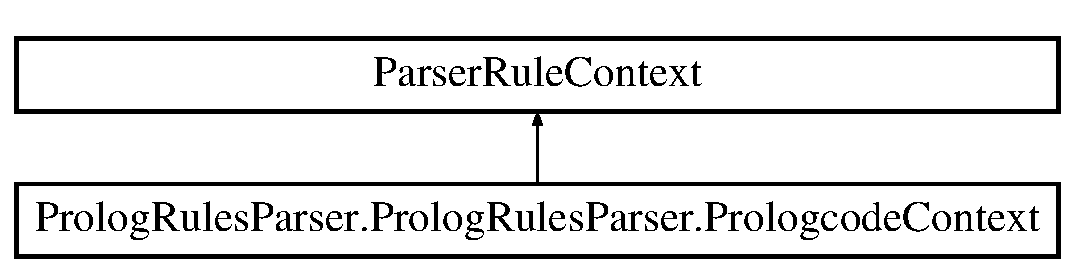
\includegraphics[height=2.000000cm]{class_prolog_rules_parser_1_1_prolog_rules_parser_1_1_prologcode_context}
\end{center}
\end{figure}
\subsection*{Public Member Functions}
\begin{DoxyCompactItemize}
\item 
def \hyperlink{class_prolog_rules_parser_1_1_prolog_rules_parser_1_1_prologcode_context_a6f6aea39505b5ff6a59388d6cdf31d20}{\+\_\+\+\_\+init\+\_\+\+\_\+}
\item 
def \hyperlink{class_prolog_rules_parser_1_1_prolog_rules_parser_1_1_prologcode_context_a3464e8f77e5f685ce6c5515288daefd7}{prologthing}
\item 
def \hyperlink{class_prolog_rules_parser_1_1_prolog_rules_parser_1_1_prologcode_context_a608138f614b771027a20b0ad895b459c}{get\+Rule\+Index} (self)
\item 
def \hyperlink{class_prolog_rules_parser_1_1_prolog_rules_parser_1_1_prologcode_context_a69432ab3fc86b526906f3266d8e32abb}{enter\+Rule} (self, listener)
\item 
def \hyperlink{class_prolog_rules_parser_1_1_prolog_rules_parser_1_1_prologcode_context_a25525a91037c63f70d4515520c27c8fa}{exit\+Rule} (self, listener)
\end{DoxyCompactItemize}
\subsection*{Public Attributes}
\begin{DoxyCompactItemize}
\item 
\hyperlink{class_prolog_rules_parser_1_1_prolog_rules_parser_1_1_prologcode_context_aec10e505a5b74230b5f4b49a9d7da40a}{parser}
\end{DoxyCompactItemize}


\subsection{Detailed Description}


Definition at line 135 of file Prolog\+Rules\+Parser.\+py.



\subsection{Constructor \& Destructor Documentation}
\hypertarget{class_prolog_rules_parser_1_1_prolog_rules_parser_1_1_prologcode_context_a6f6aea39505b5ff6a59388d6cdf31d20}{}\index{Prolog\+Rules\+Parser\+::\+Prolog\+Rules\+Parser\+::\+Prologcode\+Context@{Prolog\+Rules\+Parser\+::\+Prolog\+Rules\+Parser\+::\+Prologcode\+Context}!\+\_\+\+\_\+init\+\_\+\+\_\+@{\+\_\+\+\_\+init\+\_\+\+\_\+}}
\index{\+\_\+\+\_\+init\+\_\+\+\_\+@{\+\_\+\+\_\+init\+\_\+\+\_\+}!Prolog\+Rules\+Parser\+::\+Prolog\+Rules\+Parser\+::\+Prologcode\+Context@{Prolog\+Rules\+Parser\+::\+Prolog\+Rules\+Parser\+::\+Prologcode\+Context}}
\subsubsection[{\+\_\+\+\_\+init\+\_\+\+\_\+}]{\setlength{\rightskip}{0pt plus 5cm}def Prolog\+Rules\+Parser.\+Prolog\+Rules\+Parser.\+Prologcode\+Context.\+\_\+\+\_\+init\+\_\+\+\_\+ (
\begin{DoxyParamCaption}
\item[{}]{self, }
\item[{}]{parser, }
\item[{}]{parent = {\ttfamily None}, }
\item[{}]{invoking\+State = {\ttfamily -\/1}}
\end{DoxyParamCaption}
)}\label{class_prolog_rules_parser_1_1_prolog_rules_parser_1_1_prologcode_context_a6f6aea39505b5ff6a59388d6cdf31d20}


Definition at line 137 of file Prolog\+Rules\+Parser.\+py.



\subsection{Member Function Documentation}
\hypertarget{class_prolog_rules_parser_1_1_prolog_rules_parser_1_1_prologcode_context_a69432ab3fc86b526906f3266d8e32abb}{}\index{Prolog\+Rules\+Parser\+::\+Prolog\+Rules\+Parser\+::\+Prologcode\+Context@{Prolog\+Rules\+Parser\+::\+Prolog\+Rules\+Parser\+::\+Prologcode\+Context}!enter\+Rule@{enter\+Rule}}
\index{enter\+Rule@{enter\+Rule}!Prolog\+Rules\+Parser\+::\+Prolog\+Rules\+Parser\+::\+Prologcode\+Context@{Prolog\+Rules\+Parser\+::\+Prolog\+Rules\+Parser\+::\+Prologcode\+Context}}
\subsubsection[{enter\+Rule}]{\setlength{\rightskip}{0pt plus 5cm}def Prolog\+Rules\+Parser.\+Prolog\+Rules\+Parser.\+Prologcode\+Context.\+enter\+Rule (
\begin{DoxyParamCaption}
\item[{}]{self, }
\item[{}]{listener}
\end{DoxyParamCaption}
)}\label{class_prolog_rules_parser_1_1_prolog_rules_parser_1_1_prologcode_context_a69432ab3fc86b526906f3266d8e32abb}


Definition at line 151 of file Prolog\+Rules\+Parser.\+py.

\hypertarget{class_prolog_rules_parser_1_1_prolog_rules_parser_1_1_prologcode_context_a25525a91037c63f70d4515520c27c8fa}{}\index{Prolog\+Rules\+Parser\+::\+Prolog\+Rules\+Parser\+::\+Prologcode\+Context@{Prolog\+Rules\+Parser\+::\+Prolog\+Rules\+Parser\+::\+Prologcode\+Context}!exit\+Rule@{exit\+Rule}}
\index{exit\+Rule@{exit\+Rule}!Prolog\+Rules\+Parser\+::\+Prolog\+Rules\+Parser\+::\+Prologcode\+Context@{Prolog\+Rules\+Parser\+::\+Prolog\+Rules\+Parser\+::\+Prologcode\+Context}}
\subsubsection[{exit\+Rule}]{\setlength{\rightskip}{0pt plus 5cm}def Prolog\+Rules\+Parser.\+Prolog\+Rules\+Parser.\+Prologcode\+Context.\+exit\+Rule (
\begin{DoxyParamCaption}
\item[{}]{self, }
\item[{}]{listener}
\end{DoxyParamCaption}
)}\label{class_prolog_rules_parser_1_1_prolog_rules_parser_1_1_prologcode_context_a25525a91037c63f70d4515520c27c8fa}


Definition at line 155 of file Prolog\+Rules\+Parser.\+py.

\hypertarget{class_prolog_rules_parser_1_1_prolog_rules_parser_1_1_prologcode_context_a608138f614b771027a20b0ad895b459c}{}\index{Prolog\+Rules\+Parser\+::\+Prolog\+Rules\+Parser\+::\+Prologcode\+Context@{Prolog\+Rules\+Parser\+::\+Prolog\+Rules\+Parser\+::\+Prologcode\+Context}!get\+Rule\+Index@{get\+Rule\+Index}}
\index{get\+Rule\+Index@{get\+Rule\+Index}!Prolog\+Rules\+Parser\+::\+Prolog\+Rules\+Parser\+::\+Prologcode\+Context@{Prolog\+Rules\+Parser\+::\+Prolog\+Rules\+Parser\+::\+Prologcode\+Context}}
\subsubsection[{get\+Rule\+Index}]{\setlength{\rightskip}{0pt plus 5cm}def Prolog\+Rules\+Parser.\+Prolog\+Rules\+Parser.\+Prologcode\+Context.\+get\+Rule\+Index (
\begin{DoxyParamCaption}
\item[{}]{self}
\end{DoxyParamCaption}
)}\label{class_prolog_rules_parser_1_1_prolog_rules_parser_1_1_prologcode_context_a608138f614b771027a20b0ad895b459c}


Definition at line 148 of file Prolog\+Rules\+Parser.\+py.

\hypertarget{class_prolog_rules_parser_1_1_prolog_rules_parser_1_1_prologcode_context_a3464e8f77e5f685ce6c5515288daefd7}{}\index{Prolog\+Rules\+Parser\+::\+Prolog\+Rules\+Parser\+::\+Prologcode\+Context@{Prolog\+Rules\+Parser\+::\+Prolog\+Rules\+Parser\+::\+Prologcode\+Context}!prologthing@{prologthing}}
\index{prologthing@{prologthing}!Prolog\+Rules\+Parser\+::\+Prolog\+Rules\+Parser\+::\+Prologcode\+Context@{Prolog\+Rules\+Parser\+::\+Prolog\+Rules\+Parser\+::\+Prologcode\+Context}}
\subsubsection[{prologthing}]{\setlength{\rightskip}{0pt plus 5cm}def Prolog\+Rules\+Parser.\+Prolog\+Rules\+Parser.\+Prologcode\+Context.\+prologthing (
\begin{DoxyParamCaption}
\item[{}]{self, }
\item[{}]{i = {\ttfamily None}}
\end{DoxyParamCaption}
)}\label{class_prolog_rules_parser_1_1_prolog_rules_parser_1_1_prologcode_context_a3464e8f77e5f685ce6c5515288daefd7}


Definition at line 141 of file Prolog\+Rules\+Parser.\+py.



\subsection{Member Data Documentation}
\hypertarget{class_prolog_rules_parser_1_1_prolog_rules_parser_1_1_prologcode_context_aec10e505a5b74230b5f4b49a9d7da40a}{}\index{Prolog\+Rules\+Parser\+::\+Prolog\+Rules\+Parser\+::\+Prologcode\+Context@{Prolog\+Rules\+Parser\+::\+Prolog\+Rules\+Parser\+::\+Prologcode\+Context}!parser@{parser}}
\index{parser@{parser}!Prolog\+Rules\+Parser\+::\+Prolog\+Rules\+Parser\+::\+Prologcode\+Context@{Prolog\+Rules\+Parser\+::\+Prolog\+Rules\+Parser\+::\+Prologcode\+Context}}
\subsubsection[{parser}]{\setlength{\rightskip}{0pt plus 5cm}Prolog\+Rules\+Parser.\+Prolog\+Rules\+Parser.\+Prologcode\+Context.\+parser}\label{class_prolog_rules_parser_1_1_prolog_rules_parser_1_1_prologcode_context_aec10e505a5b74230b5f4b49a9d7da40a}


Definition at line 139 of file Prolog\+Rules\+Parser.\+py.



The documentation for this class was generated from the following file\+:\begin{DoxyCompactItemize}
\item 
\hyperlink{_prolog_rules_parser_8py}{Prolog\+Rules\+Parser.\+py}\end{DoxyCompactItemize}

\hypertarget{class_prolog_rules_parser_1_1_prolog_rules_parser_1_1_prologrule_context}{}\section{Prolog\+Rules\+Parser.\+Prolog\+Rules\+Parser.\+Prologrule\+Context Class Reference}
\label{class_prolog_rules_parser_1_1_prolog_rules_parser_1_1_prologrule_context}\index{Prolog\+Rules\+Parser.\+Prolog\+Rules\+Parser.\+Prologrule\+Context@{Prolog\+Rules\+Parser.\+Prolog\+Rules\+Parser.\+Prologrule\+Context}}
Inheritance diagram for Prolog\+Rules\+Parser.\+Prolog\+Rules\+Parser.\+Prologrule\+Context\+:\begin{figure}[H]
\begin{center}
\leavevmode
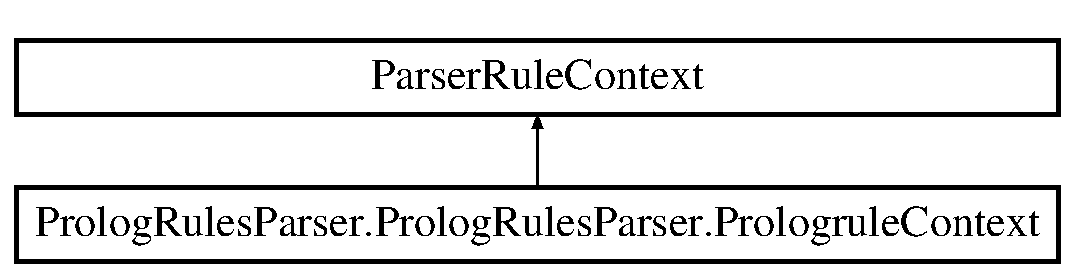
\includegraphics[height=2.000000cm]{class_prolog_rules_parser_1_1_prolog_rules_parser_1_1_prologrule_context}
\end{center}
\end{figure}
\subsection*{Public Member Functions}
\begin{DoxyCompactItemize}
\item 
def \hyperlink{class_prolog_rules_parser_1_1_prolog_rules_parser_1_1_prologrule_context_ab19a9d38ed5129b9e826422b5c9d6f35}{\+\_\+\+\_\+init\+\_\+\+\_\+}
\item 
def \hyperlink{class_prolog_rules_parser_1_1_prolog_rules_parser_1_1_prologrule_context_ab10a3a8deaee8b4cd099bb408b487fd0}{rulebody} (self)
\item 
def \hyperlink{class_prolog_rules_parser_1_1_prolog_rules_parser_1_1_prologrule_context_a382f279f2235ff7882b00ca4f57e8321}{predicate} (self)
\item 
def \hyperlink{class_prolog_rules_parser_1_1_prolog_rules_parser_1_1_prologrule_context_a9b98ac8c293cf497a0d1004e11d724b6}{get\+Rule\+Index} (self)
\item 
def \hyperlink{class_prolog_rules_parser_1_1_prolog_rules_parser_1_1_prologrule_context_a08ce20c403149023fba5207048089bd0}{enter\+Rule} (self, listener)
\item 
def \hyperlink{class_prolog_rules_parser_1_1_prolog_rules_parser_1_1_prologrule_context_ab6fa5a4a6460dcb27b4d37f62355a920}{exit\+Rule} (self, listener)
\end{DoxyCompactItemize}
\subsection*{Public Attributes}
\begin{DoxyCompactItemize}
\item 
\hyperlink{class_prolog_rules_parser_1_1_prolog_rules_parser_1_1_prologrule_context_ad0f4325fbdf95195c96853643e159ecb}{parser}
\end{DoxyCompactItemize}


\subsection{Detailed Description}


Definition at line 397 of file Prolog\+Rules\+Parser.\+py.



\subsection{Constructor \& Destructor Documentation}
\hypertarget{class_prolog_rules_parser_1_1_prolog_rules_parser_1_1_prologrule_context_ab19a9d38ed5129b9e826422b5c9d6f35}{}\index{Prolog\+Rules\+Parser\+::\+Prolog\+Rules\+Parser\+::\+Prologrule\+Context@{Prolog\+Rules\+Parser\+::\+Prolog\+Rules\+Parser\+::\+Prologrule\+Context}!\+\_\+\+\_\+init\+\_\+\+\_\+@{\+\_\+\+\_\+init\+\_\+\+\_\+}}
\index{\+\_\+\+\_\+init\+\_\+\+\_\+@{\+\_\+\+\_\+init\+\_\+\+\_\+}!Prolog\+Rules\+Parser\+::\+Prolog\+Rules\+Parser\+::\+Prologrule\+Context@{Prolog\+Rules\+Parser\+::\+Prolog\+Rules\+Parser\+::\+Prologrule\+Context}}
\subsubsection[{\+\_\+\+\_\+init\+\_\+\+\_\+}]{\setlength{\rightskip}{0pt plus 5cm}def Prolog\+Rules\+Parser.\+Prolog\+Rules\+Parser.\+Prologrule\+Context.\+\_\+\+\_\+init\+\_\+\+\_\+ (
\begin{DoxyParamCaption}
\item[{}]{self, }
\item[{}]{parser, }
\item[{}]{parent = {\ttfamily None}, }
\item[{}]{invoking\+State = {\ttfamily -\/1}}
\end{DoxyParamCaption}
)}\label{class_prolog_rules_parser_1_1_prolog_rules_parser_1_1_prologrule_context_ab19a9d38ed5129b9e826422b5c9d6f35}


Definition at line 399 of file Prolog\+Rules\+Parser.\+py.



\subsection{Member Function Documentation}
\hypertarget{class_prolog_rules_parser_1_1_prolog_rules_parser_1_1_prologrule_context_a08ce20c403149023fba5207048089bd0}{}\index{Prolog\+Rules\+Parser\+::\+Prolog\+Rules\+Parser\+::\+Prologrule\+Context@{Prolog\+Rules\+Parser\+::\+Prolog\+Rules\+Parser\+::\+Prologrule\+Context}!enter\+Rule@{enter\+Rule}}
\index{enter\+Rule@{enter\+Rule}!Prolog\+Rules\+Parser\+::\+Prolog\+Rules\+Parser\+::\+Prologrule\+Context@{Prolog\+Rules\+Parser\+::\+Prolog\+Rules\+Parser\+::\+Prologrule\+Context}}
\subsubsection[{enter\+Rule}]{\setlength{\rightskip}{0pt plus 5cm}def Prolog\+Rules\+Parser.\+Prolog\+Rules\+Parser.\+Prologrule\+Context.\+enter\+Rule (
\begin{DoxyParamCaption}
\item[{}]{self, }
\item[{}]{listener}
\end{DoxyParamCaption}
)}\label{class_prolog_rules_parser_1_1_prolog_rules_parser_1_1_prologrule_context_a08ce20c403149023fba5207048089bd0}


Definition at line 414 of file Prolog\+Rules\+Parser.\+py.

\hypertarget{class_prolog_rules_parser_1_1_prolog_rules_parser_1_1_prologrule_context_ab6fa5a4a6460dcb27b4d37f62355a920}{}\index{Prolog\+Rules\+Parser\+::\+Prolog\+Rules\+Parser\+::\+Prologrule\+Context@{Prolog\+Rules\+Parser\+::\+Prolog\+Rules\+Parser\+::\+Prologrule\+Context}!exit\+Rule@{exit\+Rule}}
\index{exit\+Rule@{exit\+Rule}!Prolog\+Rules\+Parser\+::\+Prolog\+Rules\+Parser\+::\+Prologrule\+Context@{Prolog\+Rules\+Parser\+::\+Prolog\+Rules\+Parser\+::\+Prologrule\+Context}}
\subsubsection[{exit\+Rule}]{\setlength{\rightskip}{0pt plus 5cm}def Prolog\+Rules\+Parser.\+Prolog\+Rules\+Parser.\+Prologrule\+Context.\+exit\+Rule (
\begin{DoxyParamCaption}
\item[{}]{self, }
\item[{}]{listener}
\end{DoxyParamCaption}
)}\label{class_prolog_rules_parser_1_1_prolog_rules_parser_1_1_prologrule_context_ab6fa5a4a6460dcb27b4d37f62355a920}


Definition at line 418 of file Prolog\+Rules\+Parser.\+py.

\hypertarget{class_prolog_rules_parser_1_1_prolog_rules_parser_1_1_prologrule_context_a9b98ac8c293cf497a0d1004e11d724b6}{}\index{Prolog\+Rules\+Parser\+::\+Prolog\+Rules\+Parser\+::\+Prologrule\+Context@{Prolog\+Rules\+Parser\+::\+Prolog\+Rules\+Parser\+::\+Prologrule\+Context}!get\+Rule\+Index@{get\+Rule\+Index}}
\index{get\+Rule\+Index@{get\+Rule\+Index}!Prolog\+Rules\+Parser\+::\+Prolog\+Rules\+Parser\+::\+Prologrule\+Context@{Prolog\+Rules\+Parser\+::\+Prolog\+Rules\+Parser\+::\+Prologrule\+Context}}
\subsubsection[{get\+Rule\+Index}]{\setlength{\rightskip}{0pt plus 5cm}def Prolog\+Rules\+Parser.\+Prolog\+Rules\+Parser.\+Prologrule\+Context.\+get\+Rule\+Index (
\begin{DoxyParamCaption}
\item[{}]{self}
\end{DoxyParamCaption}
)}\label{class_prolog_rules_parser_1_1_prolog_rules_parser_1_1_prologrule_context_a9b98ac8c293cf497a0d1004e11d724b6}


Definition at line 411 of file Prolog\+Rules\+Parser.\+py.

\hypertarget{class_prolog_rules_parser_1_1_prolog_rules_parser_1_1_prologrule_context_a382f279f2235ff7882b00ca4f57e8321}{}\index{Prolog\+Rules\+Parser\+::\+Prolog\+Rules\+Parser\+::\+Prologrule\+Context@{Prolog\+Rules\+Parser\+::\+Prolog\+Rules\+Parser\+::\+Prologrule\+Context}!predicate@{predicate}}
\index{predicate@{predicate}!Prolog\+Rules\+Parser\+::\+Prolog\+Rules\+Parser\+::\+Prologrule\+Context@{Prolog\+Rules\+Parser\+::\+Prolog\+Rules\+Parser\+::\+Prologrule\+Context}}
\subsubsection[{predicate}]{\setlength{\rightskip}{0pt plus 5cm}def Prolog\+Rules\+Parser.\+Prolog\+Rules\+Parser.\+Prologrule\+Context.\+predicate (
\begin{DoxyParamCaption}
\item[{}]{self}
\end{DoxyParamCaption}
)}\label{class_prolog_rules_parser_1_1_prolog_rules_parser_1_1_prologrule_context_a382f279f2235ff7882b00ca4f57e8321}


Definition at line 407 of file Prolog\+Rules\+Parser.\+py.

\hypertarget{class_prolog_rules_parser_1_1_prolog_rules_parser_1_1_prologrule_context_ab10a3a8deaee8b4cd099bb408b487fd0}{}\index{Prolog\+Rules\+Parser\+::\+Prolog\+Rules\+Parser\+::\+Prologrule\+Context@{Prolog\+Rules\+Parser\+::\+Prolog\+Rules\+Parser\+::\+Prologrule\+Context}!rulebody@{rulebody}}
\index{rulebody@{rulebody}!Prolog\+Rules\+Parser\+::\+Prolog\+Rules\+Parser\+::\+Prologrule\+Context@{Prolog\+Rules\+Parser\+::\+Prolog\+Rules\+Parser\+::\+Prologrule\+Context}}
\subsubsection[{rulebody}]{\setlength{\rightskip}{0pt plus 5cm}def Prolog\+Rules\+Parser.\+Prolog\+Rules\+Parser.\+Prologrule\+Context.\+rulebody (
\begin{DoxyParamCaption}
\item[{}]{self}
\end{DoxyParamCaption}
)}\label{class_prolog_rules_parser_1_1_prolog_rules_parser_1_1_prologrule_context_ab10a3a8deaee8b4cd099bb408b487fd0}


Definition at line 403 of file Prolog\+Rules\+Parser.\+py.



\subsection{Member Data Documentation}
\hypertarget{class_prolog_rules_parser_1_1_prolog_rules_parser_1_1_prologrule_context_ad0f4325fbdf95195c96853643e159ecb}{}\index{Prolog\+Rules\+Parser\+::\+Prolog\+Rules\+Parser\+::\+Prologrule\+Context@{Prolog\+Rules\+Parser\+::\+Prolog\+Rules\+Parser\+::\+Prologrule\+Context}!parser@{parser}}
\index{parser@{parser}!Prolog\+Rules\+Parser\+::\+Prolog\+Rules\+Parser\+::\+Prologrule\+Context@{Prolog\+Rules\+Parser\+::\+Prolog\+Rules\+Parser\+::\+Prologrule\+Context}}
\subsubsection[{parser}]{\setlength{\rightskip}{0pt plus 5cm}Prolog\+Rules\+Parser.\+Prolog\+Rules\+Parser.\+Prologrule\+Context.\+parser}\label{class_prolog_rules_parser_1_1_prolog_rules_parser_1_1_prologrule_context_ad0f4325fbdf95195c96853643e159ecb}


Definition at line 401 of file Prolog\+Rules\+Parser.\+py.



The documentation for this class was generated from the following file\+:\begin{DoxyCompactItemize}
\item 
\hyperlink{_prolog_rules_parser_8py}{Prolog\+Rules\+Parser.\+py}\end{DoxyCompactItemize}

\hypertarget{class_prolog_rules_lexer_1_1_prolog_rules_lexer}{}\section{Prolog\+Rules\+Lexer.\+Prolog\+Rules\+Lexer Class Reference}
\label{class_prolog_rules_lexer_1_1_prolog_rules_lexer}\index{Prolog\+Rules\+Lexer.\+Prolog\+Rules\+Lexer@{Prolog\+Rules\+Lexer.\+Prolog\+Rules\+Lexer}}
Inheritance diagram for Prolog\+Rules\+Lexer.\+Prolog\+Rules\+Lexer\+:\begin{figure}[H]
\begin{center}
\leavevmode
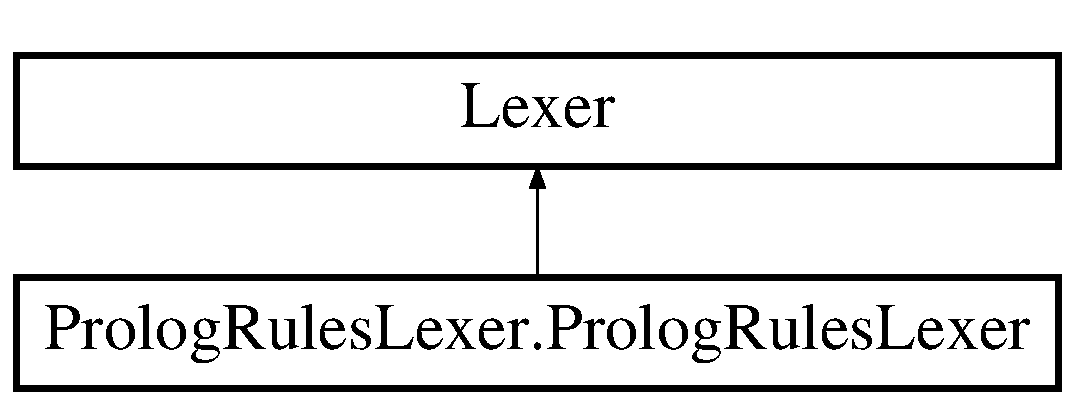
\includegraphics[height=2.000000cm]{class_prolog_rules_lexer_1_1_prolog_rules_lexer}
\end{center}
\end{figure}
\subsection*{Public Member Functions}
\begin{DoxyCompactItemize}
\item 
def \hyperlink{class_prolog_rules_lexer_1_1_prolog_rules_lexer_ad395b7b961012e4ae227eaa4b94147f7}{\+\_\+\+\_\+init\+\_\+\+\_\+}
\end{DoxyCompactItemize}
\subsection*{Static Public Attributes}
\begin{DoxyCompactItemize}
\item 
tuple \hyperlink{class_prolog_rules_lexer_1_1_prolog_rules_lexer_a938947ed2aec1cfc09c094ce44bd832b}{atn} = A\+T\+N\+Deserializer()
\item 
list \hyperlink{class_prolog_rules_lexer_1_1_prolog_rules_lexer_aa54e09333e7fafa3cde349fa87406924}{decisions\+To\+D\+F\+A} = \mbox{[} D\+F\+A(ds, i) for i, ds in enumerate(atn.\+decision\+To\+State) \mbox{]}
\item 
int \hyperlink{class_prolog_rules_lexer_1_1_prolog_rules_lexer_a6325b4258e81c531ac7cd5e46c0fde86}{T\+\_\+\+\_\+8} = 1
\item 
int \hyperlink{class_prolog_rules_lexer_1_1_prolog_rules_lexer_a048b46715d9de3b9cb895602680ef8ba}{T\+\_\+\+\_\+7} = 2
\item 
int \hyperlink{class_prolog_rules_lexer_1_1_prolog_rules_lexer_a7918ad929c34481ba9c1fccf0dc2049b}{T\+\_\+\+\_\+6} = 3
\item 
int \hyperlink{class_prolog_rules_lexer_1_1_prolog_rules_lexer_a0651d9aa3905f40e3e4efe27a2d0da3b}{T\+\_\+\+\_\+5} = 4
\item 
int \hyperlink{class_prolog_rules_lexer_1_1_prolog_rules_lexer_af2e6d8f610c091ed1237a1036fa27cf5}{T\+\_\+\+\_\+4} = 5
\item 
int \hyperlink{class_prolog_rules_lexer_1_1_prolog_rules_lexer_a30d769d7e6e0d33ce068265a838e5652}{T\+\_\+\+\_\+3} = 6
\item 
int \hyperlink{class_prolog_rules_lexer_1_1_prolog_rules_lexer_a8a043ea7c358f584213d18fcbc020d7f}{T\+\_\+\+\_\+2} = 7
\item 
int \hyperlink{class_prolog_rules_lexer_1_1_prolog_rules_lexer_a1d28a6546ce8a66389e42a9768b7b88b}{T\+\_\+\+\_\+1} = 8
\item 
int \hyperlink{class_prolog_rules_lexer_1_1_prolog_rules_lexer_a72a26fe003fdf57c9955238bbb237304}{T\+\_\+\+\_\+0} = 9
\item 
int \hyperlink{class_prolog_rules_lexer_1_1_prolog_rules_lexer_a091be41b1881614a1c583f2a5948e5b4}{N\+U\+M\+B\+E\+R} = 10
\item 
int \hyperlink{class_prolog_rules_lexer_1_1_prolog_rules_lexer_acf0cf5342114237d04f9409fab63887f}{R\+E\+L\+O\+P\+E\+R\+A\+T\+O\+R} = 11
\item 
int \hyperlink{class_prolog_rules_lexer_1_1_prolog_rules_lexer_a2a8ca9d1479d198d15fec094826e97fa}{O\+P\+E\+R\+A\+T\+O\+R} = 12
\item 
int \hyperlink{class_prolog_rules_lexer_1_1_prolog_rules_lexer_a32b617c2545824c32efc85efcbe06555}{W\+O\+R\+D} = 13
\item 
int \hyperlink{class_prolog_rules_lexer_1_1_prolog_rules_lexer_a57ccd36c7cbed70be368e17aa58caa8a}{C\+O\+M\+M\+E\+N\+T} = 14
\item 
int \hyperlink{class_prolog_rules_lexer_1_1_prolog_rules_lexer_a523e5f38e4d90961b74632dbfb8dee04}{W\+S} = 15
\item 
list \hyperlink{class_prolog_rules_lexer_1_1_prolog_rules_lexer_a85254ebf6e692330044d02a645d16f03}{mode\+Names} = \mbox{[} u\char`\"{}D\+E\+F\+A\+U\+L\+T\+\_\+\+M\+O\+D\+E\char`\"{} \mbox{]}
\item 
list \hyperlink{class_prolog_rules_lexer_1_1_prolog_rules_lexer_a233edda628c3aef92186c932b2572c21}{token\+Names}
\item 
list \hyperlink{class_prolog_rules_lexer_1_1_prolog_rules_lexer_aba72ee9a111abf678a06861eca7d2561}{rule\+Names}
\item 
string \hyperlink{class_prolog_rules_lexer_1_1_prolog_rules_lexer_ae2c3a72d3fdca809a1dc24859361641b}{grammar\+File\+Name} = u\char`\"{}Prolog\+Rules.\+g4\char`\"{}
\end{DoxyCompactItemize}


\subsection{Detailed Description}


Definition at line 47 of file Prolog\+Rules\+Lexer.\+py.



\subsection{Constructor \& Destructor Documentation}
\hypertarget{class_prolog_rules_lexer_1_1_prolog_rules_lexer_ad395b7b961012e4ae227eaa4b94147f7}{}\index{Prolog\+Rules\+Lexer\+::\+Prolog\+Rules\+Lexer@{Prolog\+Rules\+Lexer\+::\+Prolog\+Rules\+Lexer}!\+\_\+\+\_\+init\+\_\+\+\_\+@{\+\_\+\+\_\+init\+\_\+\+\_\+}}
\index{\+\_\+\+\_\+init\+\_\+\+\_\+@{\+\_\+\+\_\+init\+\_\+\+\_\+}!Prolog\+Rules\+Lexer\+::\+Prolog\+Rules\+Lexer@{Prolog\+Rules\+Lexer\+::\+Prolog\+Rules\+Lexer}}
\subsubsection[{\+\_\+\+\_\+init\+\_\+\+\_\+}]{\setlength{\rightskip}{0pt plus 5cm}def Prolog\+Rules\+Lexer.\+Prolog\+Rules\+Lexer.\+\_\+\+\_\+init\+\_\+\+\_\+ (
\begin{DoxyParamCaption}
\item[{}]{self, }
\item[{}]{input = {\ttfamily None}}
\end{DoxyParamCaption}
)}\label{class_prolog_rules_lexer_1_1_prolog_rules_lexer_ad395b7b961012e4ae227eaa4b94147f7}


Definition at line 83 of file Prolog\+Rules\+Lexer.\+py.



\subsection{Member Data Documentation}
\hypertarget{class_prolog_rules_lexer_1_1_prolog_rules_lexer_a938947ed2aec1cfc09c094ce44bd832b}{}\index{Prolog\+Rules\+Lexer\+::\+Prolog\+Rules\+Lexer@{Prolog\+Rules\+Lexer\+::\+Prolog\+Rules\+Lexer}!atn@{atn}}
\index{atn@{atn}!Prolog\+Rules\+Lexer\+::\+Prolog\+Rules\+Lexer@{Prolog\+Rules\+Lexer\+::\+Prolog\+Rules\+Lexer}}
\subsubsection[{atn}]{\setlength{\rightskip}{0pt plus 5cm}tuple Prolog\+Rules\+Lexer.\+Prolog\+Rules\+Lexer.\+atn = A\+T\+N\+Deserializer()\hspace{0.3cm}{\ttfamily [static]}}\label{class_prolog_rules_lexer_1_1_prolog_rules_lexer_a938947ed2aec1cfc09c094ce44bd832b}


Definition at line 49 of file Prolog\+Rules\+Lexer.\+py.

\hypertarget{class_prolog_rules_lexer_1_1_prolog_rules_lexer_a57ccd36c7cbed70be368e17aa58caa8a}{}\index{Prolog\+Rules\+Lexer\+::\+Prolog\+Rules\+Lexer@{Prolog\+Rules\+Lexer\+::\+Prolog\+Rules\+Lexer}!C\+O\+M\+M\+E\+N\+T@{C\+O\+M\+M\+E\+N\+T}}
\index{C\+O\+M\+M\+E\+N\+T@{C\+O\+M\+M\+E\+N\+T}!Prolog\+Rules\+Lexer\+::\+Prolog\+Rules\+Lexer@{Prolog\+Rules\+Lexer\+::\+Prolog\+Rules\+Lexer}}
\subsubsection[{C\+O\+M\+M\+E\+N\+T}]{\setlength{\rightskip}{0pt plus 5cm}int Prolog\+Rules\+Lexer.\+Prolog\+Rules\+Lexer.\+C\+O\+M\+M\+E\+N\+T = 14\hspace{0.3cm}{\ttfamily [static]}}\label{class_prolog_rules_lexer_1_1_prolog_rules_lexer_a57ccd36c7cbed70be368e17aa58caa8a}


Definition at line 66 of file Prolog\+Rules\+Lexer.\+py.

\hypertarget{class_prolog_rules_lexer_1_1_prolog_rules_lexer_aa54e09333e7fafa3cde349fa87406924}{}\index{Prolog\+Rules\+Lexer\+::\+Prolog\+Rules\+Lexer@{Prolog\+Rules\+Lexer\+::\+Prolog\+Rules\+Lexer}!decisions\+To\+D\+F\+A@{decisions\+To\+D\+F\+A}}
\index{decisions\+To\+D\+F\+A@{decisions\+To\+D\+F\+A}!Prolog\+Rules\+Lexer\+::\+Prolog\+Rules\+Lexer@{Prolog\+Rules\+Lexer\+::\+Prolog\+Rules\+Lexer}}
\subsubsection[{decisions\+To\+D\+F\+A}]{\setlength{\rightskip}{0pt plus 5cm}list Prolog\+Rules\+Lexer.\+Prolog\+Rules\+Lexer.\+decisions\+To\+D\+F\+A = \mbox{[} D\+F\+A(ds, i) for i, ds in enumerate(atn.\+decision\+To\+State) \mbox{]}\hspace{0.3cm}{\ttfamily [static]}}\label{class_prolog_rules_lexer_1_1_prolog_rules_lexer_aa54e09333e7fafa3cde349fa87406924}


Definition at line 51 of file Prolog\+Rules\+Lexer.\+py.

\hypertarget{class_prolog_rules_lexer_1_1_prolog_rules_lexer_ae2c3a72d3fdca809a1dc24859361641b}{}\index{Prolog\+Rules\+Lexer\+::\+Prolog\+Rules\+Lexer@{Prolog\+Rules\+Lexer\+::\+Prolog\+Rules\+Lexer}!grammar\+File\+Name@{grammar\+File\+Name}}
\index{grammar\+File\+Name@{grammar\+File\+Name}!Prolog\+Rules\+Lexer\+::\+Prolog\+Rules\+Lexer@{Prolog\+Rules\+Lexer\+::\+Prolog\+Rules\+Lexer}}
\subsubsection[{grammar\+File\+Name}]{\setlength{\rightskip}{0pt plus 5cm}string Prolog\+Rules\+Lexer.\+Prolog\+Rules\+Lexer.\+grammar\+File\+Name = u\char`\"{}Prolog\+Rules.\+g4\char`\"{}\hspace{0.3cm}{\ttfamily [static]}}\label{class_prolog_rules_lexer_1_1_prolog_rules_lexer_ae2c3a72d3fdca809a1dc24859361641b}


Definition at line 81 of file Prolog\+Rules\+Lexer.\+py.

\hypertarget{class_prolog_rules_lexer_1_1_prolog_rules_lexer_a85254ebf6e692330044d02a645d16f03}{}\index{Prolog\+Rules\+Lexer\+::\+Prolog\+Rules\+Lexer@{Prolog\+Rules\+Lexer\+::\+Prolog\+Rules\+Lexer}!mode\+Names@{mode\+Names}}
\index{mode\+Names@{mode\+Names}!Prolog\+Rules\+Lexer\+::\+Prolog\+Rules\+Lexer@{Prolog\+Rules\+Lexer\+::\+Prolog\+Rules\+Lexer}}
\subsubsection[{mode\+Names}]{\setlength{\rightskip}{0pt plus 5cm}list Prolog\+Rules\+Lexer.\+Prolog\+Rules\+Lexer.\+mode\+Names = \mbox{[} u\char`\"{}D\+E\+F\+A\+U\+L\+T\+\_\+\+M\+O\+D\+E\char`\"{} \mbox{]}\hspace{0.3cm}{\ttfamily [static]}}\label{class_prolog_rules_lexer_1_1_prolog_rules_lexer_a85254ebf6e692330044d02a645d16f03}


Definition at line 70 of file Prolog\+Rules\+Lexer.\+py.

\hypertarget{class_prolog_rules_lexer_1_1_prolog_rules_lexer_a091be41b1881614a1c583f2a5948e5b4}{}\index{Prolog\+Rules\+Lexer\+::\+Prolog\+Rules\+Lexer@{Prolog\+Rules\+Lexer\+::\+Prolog\+Rules\+Lexer}!N\+U\+M\+B\+E\+R@{N\+U\+M\+B\+E\+R}}
\index{N\+U\+M\+B\+E\+R@{N\+U\+M\+B\+E\+R}!Prolog\+Rules\+Lexer\+::\+Prolog\+Rules\+Lexer@{Prolog\+Rules\+Lexer\+::\+Prolog\+Rules\+Lexer}}
\subsubsection[{N\+U\+M\+B\+E\+R}]{\setlength{\rightskip}{0pt plus 5cm}int Prolog\+Rules\+Lexer.\+Prolog\+Rules\+Lexer.\+N\+U\+M\+B\+E\+R = 10\hspace{0.3cm}{\ttfamily [static]}}\label{class_prolog_rules_lexer_1_1_prolog_rules_lexer_a091be41b1881614a1c583f2a5948e5b4}


Definition at line 62 of file Prolog\+Rules\+Lexer.\+py.

\hypertarget{class_prolog_rules_lexer_1_1_prolog_rules_lexer_a2a8ca9d1479d198d15fec094826e97fa}{}\index{Prolog\+Rules\+Lexer\+::\+Prolog\+Rules\+Lexer@{Prolog\+Rules\+Lexer\+::\+Prolog\+Rules\+Lexer}!O\+P\+E\+R\+A\+T\+O\+R@{O\+P\+E\+R\+A\+T\+O\+R}}
\index{O\+P\+E\+R\+A\+T\+O\+R@{O\+P\+E\+R\+A\+T\+O\+R}!Prolog\+Rules\+Lexer\+::\+Prolog\+Rules\+Lexer@{Prolog\+Rules\+Lexer\+::\+Prolog\+Rules\+Lexer}}
\subsubsection[{O\+P\+E\+R\+A\+T\+O\+R}]{\setlength{\rightskip}{0pt plus 5cm}int Prolog\+Rules\+Lexer.\+Prolog\+Rules\+Lexer.\+O\+P\+E\+R\+A\+T\+O\+R = 12\hspace{0.3cm}{\ttfamily [static]}}\label{class_prolog_rules_lexer_1_1_prolog_rules_lexer_a2a8ca9d1479d198d15fec094826e97fa}


Definition at line 64 of file Prolog\+Rules\+Lexer.\+py.

\hypertarget{class_prolog_rules_lexer_1_1_prolog_rules_lexer_acf0cf5342114237d04f9409fab63887f}{}\index{Prolog\+Rules\+Lexer\+::\+Prolog\+Rules\+Lexer@{Prolog\+Rules\+Lexer\+::\+Prolog\+Rules\+Lexer}!R\+E\+L\+O\+P\+E\+R\+A\+T\+O\+R@{R\+E\+L\+O\+P\+E\+R\+A\+T\+O\+R}}
\index{R\+E\+L\+O\+P\+E\+R\+A\+T\+O\+R@{R\+E\+L\+O\+P\+E\+R\+A\+T\+O\+R}!Prolog\+Rules\+Lexer\+::\+Prolog\+Rules\+Lexer@{Prolog\+Rules\+Lexer\+::\+Prolog\+Rules\+Lexer}}
\subsubsection[{R\+E\+L\+O\+P\+E\+R\+A\+T\+O\+R}]{\setlength{\rightskip}{0pt plus 5cm}int Prolog\+Rules\+Lexer.\+Prolog\+Rules\+Lexer.\+R\+E\+L\+O\+P\+E\+R\+A\+T\+O\+R = 11\hspace{0.3cm}{\ttfamily [static]}}\label{class_prolog_rules_lexer_1_1_prolog_rules_lexer_acf0cf5342114237d04f9409fab63887f}


Definition at line 63 of file Prolog\+Rules\+Lexer.\+py.

\hypertarget{class_prolog_rules_lexer_1_1_prolog_rules_lexer_aba72ee9a111abf678a06861eca7d2561}{}\index{Prolog\+Rules\+Lexer\+::\+Prolog\+Rules\+Lexer@{Prolog\+Rules\+Lexer\+::\+Prolog\+Rules\+Lexer}!rule\+Names@{rule\+Names}}
\index{rule\+Names@{rule\+Names}!Prolog\+Rules\+Lexer\+::\+Prolog\+Rules\+Lexer@{Prolog\+Rules\+Lexer\+::\+Prolog\+Rules\+Lexer}}
\subsubsection[{rule\+Names}]{\setlength{\rightskip}{0pt plus 5cm}list Prolog\+Rules\+Lexer.\+Prolog\+Rules\+Lexer.\+rule\+Names\hspace{0.3cm}{\ttfamily [static]}}\label{class_prolog_rules_lexer_1_1_prolog_rules_lexer_aba72ee9a111abf678a06861eca7d2561}
{\bfseries Initial value\+:}
\begin{DoxyCode}
1 = [ \textcolor{stringliteral}{u"T\_\_8"}, \textcolor{stringliteral}{u"T\_\_7"}, \textcolor{stringliteral}{u"T\_\_6"}, \textcolor{stringliteral}{u"T\_\_5"}, \textcolor{stringliteral}{u"T\_\_4"}, \textcolor{stringliteral}{u"T\_\_3"}, 
2                   \textcolor{stringliteral}{u"T\_\_2"}, \textcolor{stringliteral}{u"T\_\_1"}, \textcolor{stringliteral}{u"T\_\_0"}, \textcolor{stringliteral}{u"NUMBER"}, \textcolor{stringliteral}{u"RELOPERATOR"}, 
3                   \textcolor{stringliteral}{u"OPERATOR"}, \textcolor{stringliteral}{u"WORD"}, \textcolor{stringliteral}{u"COMMENT"}, \textcolor{stringliteral}{u"WS"} ]
\end{DoxyCode}


Definition at line 77 of file Prolog\+Rules\+Lexer.\+py.

\hypertarget{class_prolog_rules_lexer_1_1_prolog_rules_lexer_a72a26fe003fdf57c9955238bbb237304}{}\index{Prolog\+Rules\+Lexer\+::\+Prolog\+Rules\+Lexer@{Prolog\+Rules\+Lexer\+::\+Prolog\+Rules\+Lexer}!T\+\_\+\+\_\+0@{T\+\_\+\+\_\+0}}
\index{T\+\_\+\+\_\+0@{T\+\_\+\+\_\+0}!Prolog\+Rules\+Lexer\+::\+Prolog\+Rules\+Lexer@{Prolog\+Rules\+Lexer\+::\+Prolog\+Rules\+Lexer}}
\subsubsection[{T\+\_\+\+\_\+0}]{\setlength{\rightskip}{0pt plus 5cm}int Prolog\+Rules\+Lexer.\+Prolog\+Rules\+Lexer.\+T\+\_\+\+\_\+0 = 9\hspace{0.3cm}{\ttfamily [static]}}\label{class_prolog_rules_lexer_1_1_prolog_rules_lexer_a72a26fe003fdf57c9955238bbb237304}


Definition at line 61 of file Prolog\+Rules\+Lexer.\+py.

\hypertarget{class_prolog_rules_lexer_1_1_prolog_rules_lexer_a1d28a6546ce8a66389e42a9768b7b88b}{}\index{Prolog\+Rules\+Lexer\+::\+Prolog\+Rules\+Lexer@{Prolog\+Rules\+Lexer\+::\+Prolog\+Rules\+Lexer}!T\+\_\+\+\_\+1@{T\+\_\+\+\_\+1}}
\index{T\+\_\+\+\_\+1@{T\+\_\+\+\_\+1}!Prolog\+Rules\+Lexer\+::\+Prolog\+Rules\+Lexer@{Prolog\+Rules\+Lexer\+::\+Prolog\+Rules\+Lexer}}
\subsubsection[{T\+\_\+\+\_\+1}]{\setlength{\rightskip}{0pt plus 5cm}int Prolog\+Rules\+Lexer.\+Prolog\+Rules\+Lexer.\+T\+\_\+\+\_\+1 = 8\hspace{0.3cm}{\ttfamily [static]}}\label{class_prolog_rules_lexer_1_1_prolog_rules_lexer_a1d28a6546ce8a66389e42a9768b7b88b}


Definition at line 60 of file Prolog\+Rules\+Lexer.\+py.

\hypertarget{class_prolog_rules_lexer_1_1_prolog_rules_lexer_a8a043ea7c358f584213d18fcbc020d7f}{}\index{Prolog\+Rules\+Lexer\+::\+Prolog\+Rules\+Lexer@{Prolog\+Rules\+Lexer\+::\+Prolog\+Rules\+Lexer}!T\+\_\+\+\_\+2@{T\+\_\+\+\_\+2}}
\index{T\+\_\+\+\_\+2@{T\+\_\+\+\_\+2}!Prolog\+Rules\+Lexer\+::\+Prolog\+Rules\+Lexer@{Prolog\+Rules\+Lexer\+::\+Prolog\+Rules\+Lexer}}
\subsubsection[{T\+\_\+\+\_\+2}]{\setlength{\rightskip}{0pt plus 5cm}int Prolog\+Rules\+Lexer.\+Prolog\+Rules\+Lexer.\+T\+\_\+\+\_\+2 = 7\hspace{0.3cm}{\ttfamily [static]}}\label{class_prolog_rules_lexer_1_1_prolog_rules_lexer_a8a043ea7c358f584213d18fcbc020d7f}


Definition at line 59 of file Prolog\+Rules\+Lexer.\+py.

\hypertarget{class_prolog_rules_lexer_1_1_prolog_rules_lexer_a30d769d7e6e0d33ce068265a838e5652}{}\index{Prolog\+Rules\+Lexer\+::\+Prolog\+Rules\+Lexer@{Prolog\+Rules\+Lexer\+::\+Prolog\+Rules\+Lexer}!T\+\_\+\+\_\+3@{T\+\_\+\+\_\+3}}
\index{T\+\_\+\+\_\+3@{T\+\_\+\+\_\+3}!Prolog\+Rules\+Lexer\+::\+Prolog\+Rules\+Lexer@{Prolog\+Rules\+Lexer\+::\+Prolog\+Rules\+Lexer}}
\subsubsection[{T\+\_\+\+\_\+3}]{\setlength{\rightskip}{0pt plus 5cm}int Prolog\+Rules\+Lexer.\+Prolog\+Rules\+Lexer.\+T\+\_\+\+\_\+3 = 6\hspace{0.3cm}{\ttfamily [static]}}\label{class_prolog_rules_lexer_1_1_prolog_rules_lexer_a30d769d7e6e0d33ce068265a838e5652}


Definition at line 58 of file Prolog\+Rules\+Lexer.\+py.

\hypertarget{class_prolog_rules_lexer_1_1_prolog_rules_lexer_af2e6d8f610c091ed1237a1036fa27cf5}{}\index{Prolog\+Rules\+Lexer\+::\+Prolog\+Rules\+Lexer@{Prolog\+Rules\+Lexer\+::\+Prolog\+Rules\+Lexer}!T\+\_\+\+\_\+4@{T\+\_\+\+\_\+4}}
\index{T\+\_\+\+\_\+4@{T\+\_\+\+\_\+4}!Prolog\+Rules\+Lexer\+::\+Prolog\+Rules\+Lexer@{Prolog\+Rules\+Lexer\+::\+Prolog\+Rules\+Lexer}}
\subsubsection[{T\+\_\+\+\_\+4}]{\setlength{\rightskip}{0pt plus 5cm}int Prolog\+Rules\+Lexer.\+Prolog\+Rules\+Lexer.\+T\+\_\+\+\_\+4 = 5\hspace{0.3cm}{\ttfamily [static]}}\label{class_prolog_rules_lexer_1_1_prolog_rules_lexer_af2e6d8f610c091ed1237a1036fa27cf5}


Definition at line 57 of file Prolog\+Rules\+Lexer.\+py.

\hypertarget{class_prolog_rules_lexer_1_1_prolog_rules_lexer_a0651d9aa3905f40e3e4efe27a2d0da3b}{}\index{Prolog\+Rules\+Lexer\+::\+Prolog\+Rules\+Lexer@{Prolog\+Rules\+Lexer\+::\+Prolog\+Rules\+Lexer}!T\+\_\+\+\_\+5@{T\+\_\+\+\_\+5}}
\index{T\+\_\+\+\_\+5@{T\+\_\+\+\_\+5}!Prolog\+Rules\+Lexer\+::\+Prolog\+Rules\+Lexer@{Prolog\+Rules\+Lexer\+::\+Prolog\+Rules\+Lexer}}
\subsubsection[{T\+\_\+\+\_\+5}]{\setlength{\rightskip}{0pt plus 5cm}int Prolog\+Rules\+Lexer.\+Prolog\+Rules\+Lexer.\+T\+\_\+\+\_\+5 = 4\hspace{0.3cm}{\ttfamily [static]}}\label{class_prolog_rules_lexer_1_1_prolog_rules_lexer_a0651d9aa3905f40e3e4efe27a2d0da3b}


Definition at line 56 of file Prolog\+Rules\+Lexer.\+py.

\hypertarget{class_prolog_rules_lexer_1_1_prolog_rules_lexer_a7918ad929c34481ba9c1fccf0dc2049b}{}\index{Prolog\+Rules\+Lexer\+::\+Prolog\+Rules\+Lexer@{Prolog\+Rules\+Lexer\+::\+Prolog\+Rules\+Lexer}!T\+\_\+\+\_\+6@{T\+\_\+\+\_\+6}}
\index{T\+\_\+\+\_\+6@{T\+\_\+\+\_\+6}!Prolog\+Rules\+Lexer\+::\+Prolog\+Rules\+Lexer@{Prolog\+Rules\+Lexer\+::\+Prolog\+Rules\+Lexer}}
\subsubsection[{T\+\_\+\+\_\+6}]{\setlength{\rightskip}{0pt plus 5cm}int Prolog\+Rules\+Lexer.\+Prolog\+Rules\+Lexer.\+T\+\_\+\+\_\+6 = 3\hspace{0.3cm}{\ttfamily [static]}}\label{class_prolog_rules_lexer_1_1_prolog_rules_lexer_a7918ad929c34481ba9c1fccf0dc2049b}


Definition at line 55 of file Prolog\+Rules\+Lexer.\+py.

\hypertarget{class_prolog_rules_lexer_1_1_prolog_rules_lexer_a048b46715d9de3b9cb895602680ef8ba}{}\index{Prolog\+Rules\+Lexer\+::\+Prolog\+Rules\+Lexer@{Prolog\+Rules\+Lexer\+::\+Prolog\+Rules\+Lexer}!T\+\_\+\+\_\+7@{T\+\_\+\+\_\+7}}
\index{T\+\_\+\+\_\+7@{T\+\_\+\+\_\+7}!Prolog\+Rules\+Lexer\+::\+Prolog\+Rules\+Lexer@{Prolog\+Rules\+Lexer\+::\+Prolog\+Rules\+Lexer}}
\subsubsection[{T\+\_\+\+\_\+7}]{\setlength{\rightskip}{0pt plus 5cm}int Prolog\+Rules\+Lexer.\+Prolog\+Rules\+Lexer.\+T\+\_\+\+\_\+7 = 2\hspace{0.3cm}{\ttfamily [static]}}\label{class_prolog_rules_lexer_1_1_prolog_rules_lexer_a048b46715d9de3b9cb895602680ef8ba}


Definition at line 54 of file Prolog\+Rules\+Lexer.\+py.

\hypertarget{class_prolog_rules_lexer_1_1_prolog_rules_lexer_a6325b4258e81c531ac7cd5e46c0fde86}{}\index{Prolog\+Rules\+Lexer\+::\+Prolog\+Rules\+Lexer@{Prolog\+Rules\+Lexer\+::\+Prolog\+Rules\+Lexer}!T\+\_\+\+\_\+8@{T\+\_\+\+\_\+8}}
\index{T\+\_\+\+\_\+8@{T\+\_\+\+\_\+8}!Prolog\+Rules\+Lexer\+::\+Prolog\+Rules\+Lexer@{Prolog\+Rules\+Lexer\+::\+Prolog\+Rules\+Lexer}}
\subsubsection[{T\+\_\+\+\_\+8}]{\setlength{\rightskip}{0pt plus 5cm}int Prolog\+Rules\+Lexer.\+Prolog\+Rules\+Lexer.\+T\+\_\+\+\_\+8 = 1\hspace{0.3cm}{\ttfamily [static]}}\label{class_prolog_rules_lexer_1_1_prolog_rules_lexer_a6325b4258e81c531ac7cd5e46c0fde86}


Definition at line 53 of file Prolog\+Rules\+Lexer.\+py.

\hypertarget{class_prolog_rules_lexer_1_1_prolog_rules_lexer_a233edda628c3aef92186c932b2572c21}{}\index{Prolog\+Rules\+Lexer\+::\+Prolog\+Rules\+Lexer@{Prolog\+Rules\+Lexer\+::\+Prolog\+Rules\+Lexer}!token\+Names@{token\+Names}}
\index{token\+Names@{token\+Names}!Prolog\+Rules\+Lexer\+::\+Prolog\+Rules\+Lexer@{Prolog\+Rules\+Lexer\+::\+Prolog\+Rules\+Lexer}}
\subsubsection[{token\+Names}]{\setlength{\rightskip}{0pt plus 5cm}list Prolog\+Rules\+Lexer.\+Prolog\+Rules\+Lexer.\+token\+Names\hspace{0.3cm}{\ttfamily [static]}}\label{class_prolog_rules_lexer_1_1_prolog_rules_lexer_a233edda628c3aef92186c932b2572c21}
{\bfseries Initial value\+:}
\begin{DoxyCode}
1 = [ \textcolor{stringliteral}{u"<INVALID>"},
2             \textcolor{stringliteral}{u"'\(\backslash\)\(\backslash\)u0000'"}, \textcolor{stringliteral}{u"'\(\backslash\)\(\backslash\)u0001'"}, \textcolor{stringliteral}{u"'\(\backslash\)\(\backslash\)u0002'"}, \textcolor{stringliteral}{u"'\(\backslash\)\(\backslash\)u0003'"}, \textcolor{stringliteral}{u"'\(\backslash\)\(\backslash\)u0004'"}, 
3             \textcolor{stringliteral}{u"'\(\backslash\)\(\backslash\)u0005'"}, \textcolor{stringliteral}{u"'\(\backslash\)\(\backslash\)u0006'"}, \textcolor{stringliteral}{u"'\(\backslash\)\(\backslash\)u0007'"}, \textcolor{stringliteral}{u"'\(\backslash\)b'"}, \textcolor{stringliteral}{u"'\(\backslash\)t'"}, 
4             \textcolor{stringliteral}{u"'\(\backslash\)n'"}, \textcolor{stringliteral}{u"'\(\backslash\)\(\backslash\)u000B'"}, \textcolor{stringliteral}{u"'\(\backslash\)f'"}, \textcolor{stringliteral}{u"'\(\backslash\)r'"}, \textcolor{stringliteral}{u"'\(\backslash\)\(\backslash\)u000E'"}, \textcolor{stringliteral}{u"'\(\backslash\)\(\backslash\)u000F'"} ]
\end{DoxyCode}


Definition at line 72 of file Prolog\+Rules\+Lexer.\+py.

\hypertarget{class_prolog_rules_lexer_1_1_prolog_rules_lexer_a32b617c2545824c32efc85efcbe06555}{}\index{Prolog\+Rules\+Lexer\+::\+Prolog\+Rules\+Lexer@{Prolog\+Rules\+Lexer\+::\+Prolog\+Rules\+Lexer}!W\+O\+R\+D@{W\+O\+R\+D}}
\index{W\+O\+R\+D@{W\+O\+R\+D}!Prolog\+Rules\+Lexer\+::\+Prolog\+Rules\+Lexer@{Prolog\+Rules\+Lexer\+::\+Prolog\+Rules\+Lexer}}
\subsubsection[{W\+O\+R\+D}]{\setlength{\rightskip}{0pt plus 5cm}int Prolog\+Rules\+Lexer.\+Prolog\+Rules\+Lexer.\+W\+O\+R\+D = 13\hspace{0.3cm}{\ttfamily [static]}}\label{class_prolog_rules_lexer_1_1_prolog_rules_lexer_a32b617c2545824c32efc85efcbe06555}


Definition at line 65 of file Prolog\+Rules\+Lexer.\+py.

\hypertarget{class_prolog_rules_lexer_1_1_prolog_rules_lexer_a523e5f38e4d90961b74632dbfb8dee04}{}\index{Prolog\+Rules\+Lexer\+::\+Prolog\+Rules\+Lexer@{Prolog\+Rules\+Lexer\+::\+Prolog\+Rules\+Lexer}!W\+S@{W\+S}}
\index{W\+S@{W\+S}!Prolog\+Rules\+Lexer\+::\+Prolog\+Rules\+Lexer@{Prolog\+Rules\+Lexer\+::\+Prolog\+Rules\+Lexer}}
\subsubsection[{W\+S}]{\setlength{\rightskip}{0pt plus 5cm}int Prolog\+Rules\+Lexer.\+Prolog\+Rules\+Lexer.\+W\+S = 15\hspace{0.3cm}{\ttfamily [static]}}\label{class_prolog_rules_lexer_1_1_prolog_rules_lexer_a523e5f38e4d90961b74632dbfb8dee04}


Definition at line 67 of file Prolog\+Rules\+Lexer.\+py.



The documentation for this class was generated from the following file\+:\begin{DoxyCompactItemize}
\item 
\hyperlink{_prolog_rules_lexer_8py}{Prolog\+Rules\+Lexer.\+py}\end{DoxyCompactItemize}

\hypertarget{class_prolog_rules_listener_1_1_prolog_rules_listener}{}\section{Prolog\+Rules\+Listener.\+Prolog\+Rules\+Listener Class Reference}
\label{class_prolog_rules_listener_1_1_prolog_rules_listener}\index{Prolog\+Rules\+Listener.\+Prolog\+Rules\+Listener@{Prolog\+Rules\+Listener.\+Prolog\+Rules\+Listener}}
Inheritance diagram for Prolog\+Rules\+Listener.\+Prolog\+Rules\+Listener\+:\begin{figure}[H]
\begin{center}
\leavevmode
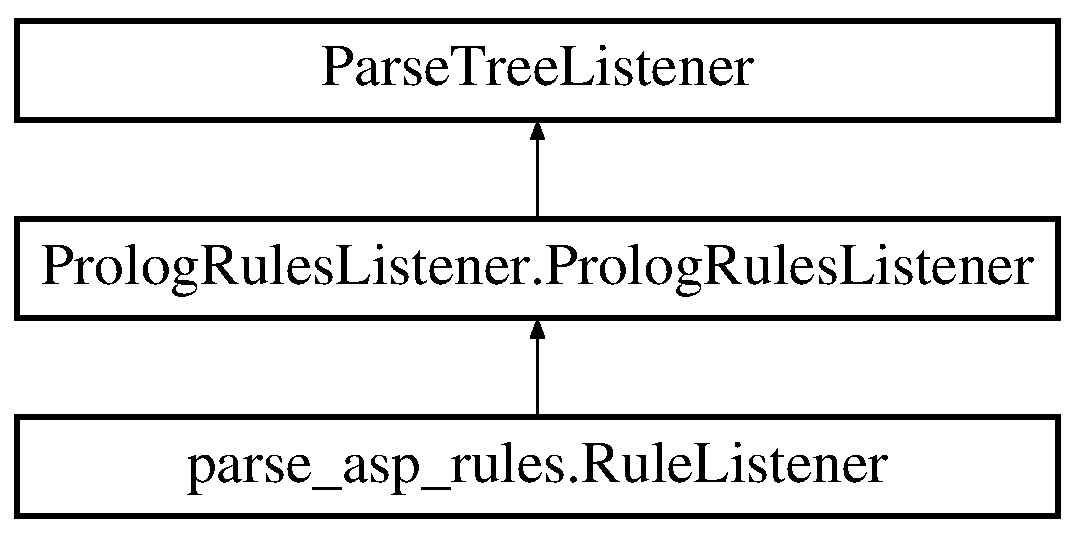
\includegraphics[height=3.000000cm]{class_prolog_rules_listener_1_1_prolog_rules_listener}
\end{center}
\end{figure}
\subsection*{Public Member Functions}
\begin{DoxyCompactItemize}
\item 
def \hyperlink{class_prolog_rules_listener_1_1_prolog_rules_listener_abbc3ef4ec1f3811b9dd194936167274f}{enter\+Atom} (self, ctx)
\item 
def \hyperlink{class_prolog_rules_listener_1_1_prolog_rules_listener_a7297673a5e8385d0c2a8ca84b575bcea}{exit\+Atom} (self, ctx)
\item 
def \hyperlink{class_prolog_rules_listener_1_1_prolog_rules_listener_a9380123ed4e178b1f5b619c4e319ea87}{enter\+Prologthing} (self, ctx)
\item 
def \hyperlink{class_prolog_rules_listener_1_1_prolog_rules_listener_a74dbe4f70addf7a4190c866d340fff39}{exit\+Prologthing} (self, ctx)
\item 
def \hyperlink{class_prolog_rules_listener_1_1_prolog_rules_listener_a60572c757692f9b6e26672d7f39501ca}{enter\+Onearg} (self, ctx)
\item 
def \hyperlink{class_prolog_rules_listener_1_1_prolog_rules_listener_aed52a06263d91850489facb20ff1f058}{exit\+Onearg} (self, ctx)
\item 
def \hyperlink{class_prolog_rules_listener_1_1_prolog_rules_listener_a5c8579ae8229948a9bf6a1ae1f0ffbad}{enter\+Condition} (self, ctx)
\item 
def \hyperlink{class_prolog_rules_listener_1_1_prolog_rules_listener_a3152b60eaee48ad32f9d60a1c02435ab}{exit\+Condition} (self, ctx)
\item 
def \hyperlink{class_prolog_rules_listener_1_1_prolog_rules_listener_a4d3020bfe94a32d003244722079db05a}{enter\+Args} (self, ctx)
\item 
def \hyperlink{class_prolog_rules_listener_1_1_prolog_rules_listener_a65394b5be33b666c136eebf315c7f271}{exit\+Args} (self, ctx)
\item 
def \hyperlink{class_prolog_rules_listener_1_1_prolog_rules_listener_ac7417bc12af903607d631814533a6d21}{enter\+Predicate} (self, ctx)
\item 
def \hyperlink{class_prolog_rules_listener_1_1_prolog_rules_listener_abc1bda2fbeb65b2962bca1a3b4ec834f}{exit\+Predicate} (self, ctx)
\item 
def \hyperlink{class_prolog_rules_listener_1_1_prolog_rules_listener_a9b9cae2c94ac78e0f14559b7d750c8e0}{enter\+Constraint} (self, ctx)
\item 
def \hyperlink{class_prolog_rules_listener_1_1_prolog_rules_listener_ae00bf77affd59f9a20d164bc371475ae}{exit\+Constraint} (self, ctx)
\item 
def \hyperlink{class_prolog_rules_listener_1_1_prolog_rules_listener_ae7d9ad27df3b8c5db7786fc2a804817e}{enter\+Prologcode} (self, ctx)
\item 
def \hyperlink{class_prolog_rules_listener_1_1_prolog_rules_listener_a8ddb03e1184656653d927a5bff2c8ccf}{exit\+Prologcode} (self, ctx)
\item 
def \hyperlink{class_prolog_rules_listener_1_1_prolog_rules_listener_a41364b82e45e6354208d0a4fe51dbdcb}{enter\+Rulebody} (self, ctx)
\item 
def \hyperlink{class_prolog_rules_listener_1_1_prolog_rules_listener_abcd51c4d81a4c71442f09647706e69cc}{exit\+Rulebody} (self, ctx)
\item 
def \hyperlink{class_prolog_rules_listener_1_1_prolog_rules_listener_a9bf027ec3af1068dce4cc80b9e27b434}{enter\+Comparator} (self, ctx)
\item 
def \hyperlink{class_prolog_rules_listener_1_1_prolog_rules_listener_a0cafd8d6a4b77b58452f056eddc90962}{exit\+Comparator} (self, ctx)
\item 
def \hyperlink{class_prolog_rules_listener_1_1_prolog_rules_listener_a425c4305f85fb7ef87fcba9299d9a8ac}{enter\+Negpred} (self, ctx)
\item 
def \hyperlink{class_prolog_rules_listener_1_1_prolog_rules_listener_a25ea2490b9ffebaea62c6863357ab94f}{exit\+Negpred} (self, ctx)
\item 
def \hyperlink{class_prolog_rules_listener_1_1_prolog_rules_listener_a6aec3841e8f4a23989b187ba84175c18}{enter\+Predcount} (self, ctx)
\item 
def \hyperlink{class_prolog_rules_listener_1_1_prolog_rules_listener_aaae8d459660fdf15cf578b24e1b011ca}{exit\+Predcount} (self, ctx)
\item 
def \hyperlink{class_prolog_rules_listener_1_1_prolog_rules_listener_a217bdafc24abf56487a962b70e5931c4}{enter\+Mathexpr} (self, ctx)
\item 
def \hyperlink{class_prolog_rules_listener_1_1_prolog_rules_listener_aec58e638995df290d2e62304988e8232}{exit\+Mathexpr} (self, ctx)
\item 
def \hyperlink{class_prolog_rules_listener_1_1_prolog_rules_listener_a976337da036f232ec05247eae3624b14}{enter\+Somerule} (self, ctx)
\item 
def \hyperlink{class_prolog_rules_listener_1_1_prolog_rules_listener_a5d12255f24bf26e1f5b4b45708967825}{exit\+Somerule} (self, ctx)
\item 
def \hyperlink{class_prolog_rules_listener_1_1_prolog_rules_listener_a66dfdd4416b749850b7444f13dd5d02d}{enter\+Fact} (self, ctx)
\item 
def \hyperlink{class_prolog_rules_listener_1_1_prolog_rules_listener_aec2344b771b8e60af49caf8de2b23d89}{exit\+Fact} (self, ctx)
\item 
def \hyperlink{class_prolog_rules_listener_1_1_prolog_rules_listener_a42ba9d55b0e22d9a462e27c2ba5f3864}{enter\+Guessrule} (self, ctx)
\item 
def \hyperlink{class_prolog_rules_listener_1_1_prolog_rules_listener_a88a498da0dab26eaf19001c0c3bbd7ca}{exit\+Guessrule} (self, ctx)
\item 
def \hyperlink{class_prolog_rules_listener_1_1_prolog_rules_listener_a2f3b751c7a22ba23e4addd31fd742665}{enter\+Prologrule} (self, ctx)
\item 
def \hyperlink{class_prolog_rules_listener_1_1_prolog_rules_listener_afb49913317076e74be143d737184407d}{exit\+Prologrule} (self, ctx)
\item 
def \hyperlink{class_prolog_rules_listener_1_1_prolog_rules_listener_a651e7f8b18e601f5aa33b49190b090cd}{enter\+Identifier} (self, ctx)
\item 
def \hyperlink{class_prolog_rules_listener_1_1_prolog_rules_listener_a1dd9ffbbc87431ba294607de6dbe8edd}{exit\+Identifier} (self, ctx)
\end{DoxyCompactItemize}


\subsection{Detailed Description}


Definition at line 5 of file Prolog\+Rules\+Listener.\+py.



\subsection{Member Function Documentation}
\hypertarget{class_prolog_rules_listener_1_1_prolog_rules_listener_a4d3020bfe94a32d003244722079db05a}{}\index{Prolog\+Rules\+Listener\+::\+Prolog\+Rules\+Listener@{Prolog\+Rules\+Listener\+::\+Prolog\+Rules\+Listener}!enter\+Args@{enter\+Args}}
\index{enter\+Args@{enter\+Args}!Prolog\+Rules\+Listener\+::\+Prolog\+Rules\+Listener@{Prolog\+Rules\+Listener\+::\+Prolog\+Rules\+Listener}}
\subsubsection[{enter\+Args}]{\setlength{\rightskip}{0pt plus 5cm}def Prolog\+Rules\+Listener.\+Prolog\+Rules\+Listener.\+enter\+Args (
\begin{DoxyParamCaption}
\item[{}]{self, }
\item[{}]{ctx}
\end{DoxyParamCaption}
)}\label{class_prolog_rules_listener_1_1_prolog_rules_listener_a4d3020bfe94a32d003244722079db05a}


Definition at line 44 of file Prolog\+Rules\+Listener.\+py.

\hypertarget{class_prolog_rules_listener_1_1_prolog_rules_listener_abbc3ef4ec1f3811b9dd194936167274f}{}\index{Prolog\+Rules\+Listener\+::\+Prolog\+Rules\+Listener@{Prolog\+Rules\+Listener\+::\+Prolog\+Rules\+Listener}!enter\+Atom@{enter\+Atom}}
\index{enter\+Atom@{enter\+Atom}!Prolog\+Rules\+Listener\+::\+Prolog\+Rules\+Listener@{Prolog\+Rules\+Listener\+::\+Prolog\+Rules\+Listener}}
\subsubsection[{enter\+Atom}]{\setlength{\rightskip}{0pt plus 5cm}def Prolog\+Rules\+Listener.\+Prolog\+Rules\+Listener.\+enter\+Atom (
\begin{DoxyParamCaption}
\item[{}]{self, }
\item[{}]{ctx}
\end{DoxyParamCaption}
)}\label{class_prolog_rules_listener_1_1_prolog_rules_listener_abbc3ef4ec1f3811b9dd194936167274f}


Definition at line 8 of file Prolog\+Rules\+Listener.\+py.

\hypertarget{class_prolog_rules_listener_1_1_prolog_rules_listener_a9bf027ec3af1068dce4cc80b9e27b434}{}\index{Prolog\+Rules\+Listener\+::\+Prolog\+Rules\+Listener@{Prolog\+Rules\+Listener\+::\+Prolog\+Rules\+Listener}!enter\+Comparator@{enter\+Comparator}}
\index{enter\+Comparator@{enter\+Comparator}!Prolog\+Rules\+Listener\+::\+Prolog\+Rules\+Listener@{Prolog\+Rules\+Listener\+::\+Prolog\+Rules\+Listener}}
\subsubsection[{enter\+Comparator}]{\setlength{\rightskip}{0pt plus 5cm}def Prolog\+Rules\+Listener.\+Prolog\+Rules\+Listener.\+enter\+Comparator (
\begin{DoxyParamCaption}
\item[{}]{self, }
\item[{}]{ctx}
\end{DoxyParamCaption}
)}\label{class_prolog_rules_listener_1_1_prolog_rules_listener_a9bf027ec3af1068dce4cc80b9e27b434}


Definition at line 89 of file Prolog\+Rules\+Listener.\+py.

\hypertarget{class_prolog_rules_listener_1_1_prolog_rules_listener_a5c8579ae8229948a9bf6a1ae1f0ffbad}{}\index{Prolog\+Rules\+Listener\+::\+Prolog\+Rules\+Listener@{Prolog\+Rules\+Listener\+::\+Prolog\+Rules\+Listener}!enter\+Condition@{enter\+Condition}}
\index{enter\+Condition@{enter\+Condition}!Prolog\+Rules\+Listener\+::\+Prolog\+Rules\+Listener@{Prolog\+Rules\+Listener\+::\+Prolog\+Rules\+Listener}}
\subsubsection[{enter\+Condition}]{\setlength{\rightskip}{0pt plus 5cm}def Prolog\+Rules\+Listener.\+Prolog\+Rules\+Listener.\+enter\+Condition (
\begin{DoxyParamCaption}
\item[{}]{self, }
\item[{}]{ctx}
\end{DoxyParamCaption}
)}\label{class_prolog_rules_listener_1_1_prolog_rules_listener_a5c8579ae8229948a9bf6a1ae1f0ffbad}


Definition at line 35 of file Prolog\+Rules\+Listener.\+py.

\hypertarget{class_prolog_rules_listener_1_1_prolog_rules_listener_a9b9cae2c94ac78e0f14559b7d750c8e0}{}\index{Prolog\+Rules\+Listener\+::\+Prolog\+Rules\+Listener@{Prolog\+Rules\+Listener\+::\+Prolog\+Rules\+Listener}!enter\+Constraint@{enter\+Constraint}}
\index{enter\+Constraint@{enter\+Constraint}!Prolog\+Rules\+Listener\+::\+Prolog\+Rules\+Listener@{Prolog\+Rules\+Listener\+::\+Prolog\+Rules\+Listener}}
\subsubsection[{enter\+Constraint}]{\setlength{\rightskip}{0pt plus 5cm}def Prolog\+Rules\+Listener.\+Prolog\+Rules\+Listener.\+enter\+Constraint (
\begin{DoxyParamCaption}
\item[{}]{self, }
\item[{}]{ctx}
\end{DoxyParamCaption}
)}\label{class_prolog_rules_listener_1_1_prolog_rules_listener_a9b9cae2c94ac78e0f14559b7d750c8e0}


Definition at line 62 of file Prolog\+Rules\+Listener.\+py.

\hypertarget{class_prolog_rules_listener_1_1_prolog_rules_listener_a66dfdd4416b749850b7444f13dd5d02d}{}\index{Prolog\+Rules\+Listener\+::\+Prolog\+Rules\+Listener@{Prolog\+Rules\+Listener\+::\+Prolog\+Rules\+Listener}!enter\+Fact@{enter\+Fact}}
\index{enter\+Fact@{enter\+Fact}!Prolog\+Rules\+Listener\+::\+Prolog\+Rules\+Listener@{Prolog\+Rules\+Listener\+::\+Prolog\+Rules\+Listener}}
\subsubsection[{enter\+Fact}]{\setlength{\rightskip}{0pt plus 5cm}def Prolog\+Rules\+Listener.\+Prolog\+Rules\+Listener.\+enter\+Fact (
\begin{DoxyParamCaption}
\item[{}]{self, }
\item[{}]{ctx}
\end{DoxyParamCaption}
)}\label{class_prolog_rules_listener_1_1_prolog_rules_listener_a66dfdd4416b749850b7444f13dd5d02d}


Definition at line 134 of file Prolog\+Rules\+Listener.\+py.

\hypertarget{class_prolog_rules_listener_1_1_prolog_rules_listener_a42ba9d55b0e22d9a462e27c2ba5f3864}{}\index{Prolog\+Rules\+Listener\+::\+Prolog\+Rules\+Listener@{Prolog\+Rules\+Listener\+::\+Prolog\+Rules\+Listener}!enter\+Guessrule@{enter\+Guessrule}}
\index{enter\+Guessrule@{enter\+Guessrule}!Prolog\+Rules\+Listener\+::\+Prolog\+Rules\+Listener@{Prolog\+Rules\+Listener\+::\+Prolog\+Rules\+Listener}}
\subsubsection[{enter\+Guessrule}]{\setlength{\rightskip}{0pt plus 5cm}def Prolog\+Rules\+Listener.\+Prolog\+Rules\+Listener.\+enter\+Guessrule (
\begin{DoxyParamCaption}
\item[{}]{self, }
\item[{}]{ctx}
\end{DoxyParamCaption}
)}\label{class_prolog_rules_listener_1_1_prolog_rules_listener_a42ba9d55b0e22d9a462e27c2ba5f3864}


Definition at line 143 of file Prolog\+Rules\+Listener.\+py.

\hypertarget{class_prolog_rules_listener_1_1_prolog_rules_listener_a651e7f8b18e601f5aa33b49190b090cd}{}\index{Prolog\+Rules\+Listener\+::\+Prolog\+Rules\+Listener@{Prolog\+Rules\+Listener\+::\+Prolog\+Rules\+Listener}!enter\+Identifier@{enter\+Identifier}}
\index{enter\+Identifier@{enter\+Identifier}!Prolog\+Rules\+Listener\+::\+Prolog\+Rules\+Listener@{Prolog\+Rules\+Listener\+::\+Prolog\+Rules\+Listener}}
\subsubsection[{enter\+Identifier}]{\setlength{\rightskip}{0pt plus 5cm}def Prolog\+Rules\+Listener.\+Prolog\+Rules\+Listener.\+enter\+Identifier (
\begin{DoxyParamCaption}
\item[{}]{self, }
\item[{}]{ctx}
\end{DoxyParamCaption}
)}\label{class_prolog_rules_listener_1_1_prolog_rules_listener_a651e7f8b18e601f5aa33b49190b090cd}


Definition at line 161 of file Prolog\+Rules\+Listener.\+py.

\hypertarget{class_prolog_rules_listener_1_1_prolog_rules_listener_a217bdafc24abf56487a962b70e5931c4}{}\index{Prolog\+Rules\+Listener\+::\+Prolog\+Rules\+Listener@{Prolog\+Rules\+Listener\+::\+Prolog\+Rules\+Listener}!enter\+Mathexpr@{enter\+Mathexpr}}
\index{enter\+Mathexpr@{enter\+Mathexpr}!Prolog\+Rules\+Listener\+::\+Prolog\+Rules\+Listener@{Prolog\+Rules\+Listener\+::\+Prolog\+Rules\+Listener}}
\subsubsection[{enter\+Mathexpr}]{\setlength{\rightskip}{0pt plus 5cm}def Prolog\+Rules\+Listener.\+Prolog\+Rules\+Listener.\+enter\+Mathexpr (
\begin{DoxyParamCaption}
\item[{}]{self, }
\item[{}]{ctx}
\end{DoxyParamCaption}
)}\label{class_prolog_rules_listener_1_1_prolog_rules_listener_a217bdafc24abf56487a962b70e5931c4}


Definition at line 116 of file Prolog\+Rules\+Listener.\+py.

\hypertarget{class_prolog_rules_listener_1_1_prolog_rules_listener_a425c4305f85fb7ef87fcba9299d9a8ac}{}\index{Prolog\+Rules\+Listener\+::\+Prolog\+Rules\+Listener@{Prolog\+Rules\+Listener\+::\+Prolog\+Rules\+Listener}!enter\+Negpred@{enter\+Negpred}}
\index{enter\+Negpred@{enter\+Negpred}!Prolog\+Rules\+Listener\+::\+Prolog\+Rules\+Listener@{Prolog\+Rules\+Listener\+::\+Prolog\+Rules\+Listener}}
\subsubsection[{enter\+Negpred}]{\setlength{\rightskip}{0pt plus 5cm}def Prolog\+Rules\+Listener.\+Prolog\+Rules\+Listener.\+enter\+Negpred (
\begin{DoxyParamCaption}
\item[{}]{self, }
\item[{}]{ctx}
\end{DoxyParamCaption}
)}\label{class_prolog_rules_listener_1_1_prolog_rules_listener_a425c4305f85fb7ef87fcba9299d9a8ac}


Definition at line 98 of file Prolog\+Rules\+Listener.\+py.

\hypertarget{class_prolog_rules_listener_1_1_prolog_rules_listener_a60572c757692f9b6e26672d7f39501ca}{}\index{Prolog\+Rules\+Listener\+::\+Prolog\+Rules\+Listener@{Prolog\+Rules\+Listener\+::\+Prolog\+Rules\+Listener}!enter\+Onearg@{enter\+Onearg}}
\index{enter\+Onearg@{enter\+Onearg}!Prolog\+Rules\+Listener\+::\+Prolog\+Rules\+Listener@{Prolog\+Rules\+Listener\+::\+Prolog\+Rules\+Listener}}
\subsubsection[{enter\+Onearg}]{\setlength{\rightskip}{0pt plus 5cm}def Prolog\+Rules\+Listener.\+Prolog\+Rules\+Listener.\+enter\+Onearg (
\begin{DoxyParamCaption}
\item[{}]{self, }
\item[{}]{ctx}
\end{DoxyParamCaption}
)}\label{class_prolog_rules_listener_1_1_prolog_rules_listener_a60572c757692f9b6e26672d7f39501ca}


Definition at line 26 of file Prolog\+Rules\+Listener.\+py.

\hypertarget{class_prolog_rules_listener_1_1_prolog_rules_listener_a6aec3841e8f4a23989b187ba84175c18}{}\index{Prolog\+Rules\+Listener\+::\+Prolog\+Rules\+Listener@{Prolog\+Rules\+Listener\+::\+Prolog\+Rules\+Listener}!enter\+Predcount@{enter\+Predcount}}
\index{enter\+Predcount@{enter\+Predcount}!Prolog\+Rules\+Listener\+::\+Prolog\+Rules\+Listener@{Prolog\+Rules\+Listener\+::\+Prolog\+Rules\+Listener}}
\subsubsection[{enter\+Predcount}]{\setlength{\rightskip}{0pt plus 5cm}def Prolog\+Rules\+Listener.\+Prolog\+Rules\+Listener.\+enter\+Predcount (
\begin{DoxyParamCaption}
\item[{}]{self, }
\item[{}]{ctx}
\end{DoxyParamCaption}
)}\label{class_prolog_rules_listener_1_1_prolog_rules_listener_a6aec3841e8f4a23989b187ba84175c18}


Definition at line 107 of file Prolog\+Rules\+Listener.\+py.

\hypertarget{class_prolog_rules_listener_1_1_prolog_rules_listener_ac7417bc12af903607d631814533a6d21}{}\index{Prolog\+Rules\+Listener\+::\+Prolog\+Rules\+Listener@{Prolog\+Rules\+Listener\+::\+Prolog\+Rules\+Listener}!enter\+Predicate@{enter\+Predicate}}
\index{enter\+Predicate@{enter\+Predicate}!Prolog\+Rules\+Listener\+::\+Prolog\+Rules\+Listener@{Prolog\+Rules\+Listener\+::\+Prolog\+Rules\+Listener}}
\subsubsection[{enter\+Predicate}]{\setlength{\rightskip}{0pt plus 5cm}def Prolog\+Rules\+Listener.\+Prolog\+Rules\+Listener.\+enter\+Predicate (
\begin{DoxyParamCaption}
\item[{}]{self, }
\item[{}]{ctx}
\end{DoxyParamCaption}
)}\label{class_prolog_rules_listener_1_1_prolog_rules_listener_ac7417bc12af903607d631814533a6d21}


Definition at line 53 of file Prolog\+Rules\+Listener.\+py.

\hypertarget{class_prolog_rules_listener_1_1_prolog_rules_listener_ae7d9ad27df3b8c5db7786fc2a804817e}{}\index{Prolog\+Rules\+Listener\+::\+Prolog\+Rules\+Listener@{Prolog\+Rules\+Listener\+::\+Prolog\+Rules\+Listener}!enter\+Prologcode@{enter\+Prologcode}}
\index{enter\+Prologcode@{enter\+Prologcode}!Prolog\+Rules\+Listener\+::\+Prolog\+Rules\+Listener@{Prolog\+Rules\+Listener\+::\+Prolog\+Rules\+Listener}}
\subsubsection[{enter\+Prologcode}]{\setlength{\rightskip}{0pt plus 5cm}def Prolog\+Rules\+Listener.\+Prolog\+Rules\+Listener.\+enter\+Prologcode (
\begin{DoxyParamCaption}
\item[{}]{self, }
\item[{}]{ctx}
\end{DoxyParamCaption}
)}\label{class_prolog_rules_listener_1_1_prolog_rules_listener_ae7d9ad27df3b8c5db7786fc2a804817e}


Definition at line 71 of file Prolog\+Rules\+Listener.\+py.

\hypertarget{class_prolog_rules_listener_1_1_prolog_rules_listener_a2f3b751c7a22ba23e4addd31fd742665}{}\index{Prolog\+Rules\+Listener\+::\+Prolog\+Rules\+Listener@{Prolog\+Rules\+Listener\+::\+Prolog\+Rules\+Listener}!enter\+Prologrule@{enter\+Prologrule}}
\index{enter\+Prologrule@{enter\+Prologrule}!Prolog\+Rules\+Listener\+::\+Prolog\+Rules\+Listener@{Prolog\+Rules\+Listener\+::\+Prolog\+Rules\+Listener}}
\subsubsection[{enter\+Prologrule}]{\setlength{\rightskip}{0pt plus 5cm}def Prolog\+Rules\+Listener.\+Prolog\+Rules\+Listener.\+enter\+Prologrule (
\begin{DoxyParamCaption}
\item[{}]{self, }
\item[{}]{ctx}
\end{DoxyParamCaption}
)}\label{class_prolog_rules_listener_1_1_prolog_rules_listener_a2f3b751c7a22ba23e4addd31fd742665}


Definition at line 152 of file Prolog\+Rules\+Listener.\+py.

\hypertarget{class_prolog_rules_listener_1_1_prolog_rules_listener_a9380123ed4e178b1f5b619c4e319ea87}{}\index{Prolog\+Rules\+Listener\+::\+Prolog\+Rules\+Listener@{Prolog\+Rules\+Listener\+::\+Prolog\+Rules\+Listener}!enter\+Prologthing@{enter\+Prologthing}}
\index{enter\+Prologthing@{enter\+Prologthing}!Prolog\+Rules\+Listener\+::\+Prolog\+Rules\+Listener@{Prolog\+Rules\+Listener\+::\+Prolog\+Rules\+Listener}}
\subsubsection[{enter\+Prologthing}]{\setlength{\rightskip}{0pt plus 5cm}def Prolog\+Rules\+Listener.\+Prolog\+Rules\+Listener.\+enter\+Prologthing (
\begin{DoxyParamCaption}
\item[{}]{self, }
\item[{}]{ctx}
\end{DoxyParamCaption}
)}\label{class_prolog_rules_listener_1_1_prolog_rules_listener_a9380123ed4e178b1f5b619c4e319ea87}


Definition at line 17 of file Prolog\+Rules\+Listener.\+py.

\hypertarget{class_prolog_rules_listener_1_1_prolog_rules_listener_a41364b82e45e6354208d0a4fe51dbdcb}{}\index{Prolog\+Rules\+Listener\+::\+Prolog\+Rules\+Listener@{Prolog\+Rules\+Listener\+::\+Prolog\+Rules\+Listener}!enter\+Rulebody@{enter\+Rulebody}}
\index{enter\+Rulebody@{enter\+Rulebody}!Prolog\+Rules\+Listener\+::\+Prolog\+Rules\+Listener@{Prolog\+Rules\+Listener\+::\+Prolog\+Rules\+Listener}}
\subsubsection[{enter\+Rulebody}]{\setlength{\rightskip}{0pt plus 5cm}def Prolog\+Rules\+Listener.\+Prolog\+Rules\+Listener.\+enter\+Rulebody (
\begin{DoxyParamCaption}
\item[{}]{self, }
\item[{}]{ctx}
\end{DoxyParamCaption}
)}\label{class_prolog_rules_listener_1_1_prolog_rules_listener_a41364b82e45e6354208d0a4fe51dbdcb}


Definition at line 80 of file Prolog\+Rules\+Listener.\+py.

\hypertarget{class_prolog_rules_listener_1_1_prolog_rules_listener_a976337da036f232ec05247eae3624b14}{}\index{Prolog\+Rules\+Listener\+::\+Prolog\+Rules\+Listener@{Prolog\+Rules\+Listener\+::\+Prolog\+Rules\+Listener}!enter\+Somerule@{enter\+Somerule}}
\index{enter\+Somerule@{enter\+Somerule}!Prolog\+Rules\+Listener\+::\+Prolog\+Rules\+Listener@{Prolog\+Rules\+Listener\+::\+Prolog\+Rules\+Listener}}
\subsubsection[{enter\+Somerule}]{\setlength{\rightskip}{0pt plus 5cm}def Prolog\+Rules\+Listener.\+Prolog\+Rules\+Listener.\+enter\+Somerule (
\begin{DoxyParamCaption}
\item[{}]{self, }
\item[{}]{ctx}
\end{DoxyParamCaption}
)}\label{class_prolog_rules_listener_1_1_prolog_rules_listener_a976337da036f232ec05247eae3624b14}


Definition at line 125 of file Prolog\+Rules\+Listener.\+py.

\hypertarget{class_prolog_rules_listener_1_1_prolog_rules_listener_a65394b5be33b666c136eebf315c7f271}{}\index{Prolog\+Rules\+Listener\+::\+Prolog\+Rules\+Listener@{Prolog\+Rules\+Listener\+::\+Prolog\+Rules\+Listener}!exit\+Args@{exit\+Args}}
\index{exit\+Args@{exit\+Args}!Prolog\+Rules\+Listener\+::\+Prolog\+Rules\+Listener@{Prolog\+Rules\+Listener\+::\+Prolog\+Rules\+Listener}}
\subsubsection[{exit\+Args}]{\setlength{\rightskip}{0pt plus 5cm}def Prolog\+Rules\+Listener.\+Prolog\+Rules\+Listener.\+exit\+Args (
\begin{DoxyParamCaption}
\item[{}]{self, }
\item[{}]{ctx}
\end{DoxyParamCaption}
)}\label{class_prolog_rules_listener_1_1_prolog_rules_listener_a65394b5be33b666c136eebf315c7f271}


Definition at line 48 of file Prolog\+Rules\+Listener.\+py.

\hypertarget{class_prolog_rules_listener_1_1_prolog_rules_listener_a7297673a5e8385d0c2a8ca84b575bcea}{}\index{Prolog\+Rules\+Listener\+::\+Prolog\+Rules\+Listener@{Prolog\+Rules\+Listener\+::\+Prolog\+Rules\+Listener}!exit\+Atom@{exit\+Atom}}
\index{exit\+Atom@{exit\+Atom}!Prolog\+Rules\+Listener\+::\+Prolog\+Rules\+Listener@{Prolog\+Rules\+Listener\+::\+Prolog\+Rules\+Listener}}
\subsubsection[{exit\+Atom}]{\setlength{\rightskip}{0pt plus 5cm}def Prolog\+Rules\+Listener.\+Prolog\+Rules\+Listener.\+exit\+Atom (
\begin{DoxyParamCaption}
\item[{}]{self, }
\item[{}]{ctx}
\end{DoxyParamCaption}
)}\label{class_prolog_rules_listener_1_1_prolog_rules_listener_a7297673a5e8385d0c2a8ca84b575bcea}


Definition at line 12 of file Prolog\+Rules\+Listener.\+py.

\hypertarget{class_prolog_rules_listener_1_1_prolog_rules_listener_a0cafd8d6a4b77b58452f056eddc90962}{}\index{Prolog\+Rules\+Listener\+::\+Prolog\+Rules\+Listener@{Prolog\+Rules\+Listener\+::\+Prolog\+Rules\+Listener}!exit\+Comparator@{exit\+Comparator}}
\index{exit\+Comparator@{exit\+Comparator}!Prolog\+Rules\+Listener\+::\+Prolog\+Rules\+Listener@{Prolog\+Rules\+Listener\+::\+Prolog\+Rules\+Listener}}
\subsubsection[{exit\+Comparator}]{\setlength{\rightskip}{0pt plus 5cm}def Prolog\+Rules\+Listener.\+Prolog\+Rules\+Listener.\+exit\+Comparator (
\begin{DoxyParamCaption}
\item[{}]{self, }
\item[{}]{ctx}
\end{DoxyParamCaption}
)}\label{class_prolog_rules_listener_1_1_prolog_rules_listener_a0cafd8d6a4b77b58452f056eddc90962}


Definition at line 93 of file Prolog\+Rules\+Listener.\+py.

\hypertarget{class_prolog_rules_listener_1_1_prolog_rules_listener_a3152b60eaee48ad32f9d60a1c02435ab}{}\index{Prolog\+Rules\+Listener\+::\+Prolog\+Rules\+Listener@{Prolog\+Rules\+Listener\+::\+Prolog\+Rules\+Listener}!exit\+Condition@{exit\+Condition}}
\index{exit\+Condition@{exit\+Condition}!Prolog\+Rules\+Listener\+::\+Prolog\+Rules\+Listener@{Prolog\+Rules\+Listener\+::\+Prolog\+Rules\+Listener}}
\subsubsection[{exit\+Condition}]{\setlength{\rightskip}{0pt plus 5cm}def Prolog\+Rules\+Listener.\+Prolog\+Rules\+Listener.\+exit\+Condition (
\begin{DoxyParamCaption}
\item[{}]{self, }
\item[{}]{ctx}
\end{DoxyParamCaption}
)}\label{class_prolog_rules_listener_1_1_prolog_rules_listener_a3152b60eaee48ad32f9d60a1c02435ab}


Definition at line 39 of file Prolog\+Rules\+Listener.\+py.

\hypertarget{class_prolog_rules_listener_1_1_prolog_rules_listener_ae00bf77affd59f9a20d164bc371475ae}{}\index{Prolog\+Rules\+Listener\+::\+Prolog\+Rules\+Listener@{Prolog\+Rules\+Listener\+::\+Prolog\+Rules\+Listener}!exit\+Constraint@{exit\+Constraint}}
\index{exit\+Constraint@{exit\+Constraint}!Prolog\+Rules\+Listener\+::\+Prolog\+Rules\+Listener@{Prolog\+Rules\+Listener\+::\+Prolog\+Rules\+Listener}}
\subsubsection[{exit\+Constraint}]{\setlength{\rightskip}{0pt plus 5cm}def Prolog\+Rules\+Listener.\+Prolog\+Rules\+Listener.\+exit\+Constraint (
\begin{DoxyParamCaption}
\item[{}]{self, }
\item[{}]{ctx}
\end{DoxyParamCaption}
)}\label{class_prolog_rules_listener_1_1_prolog_rules_listener_ae00bf77affd59f9a20d164bc371475ae}


Definition at line 66 of file Prolog\+Rules\+Listener.\+py.

\hypertarget{class_prolog_rules_listener_1_1_prolog_rules_listener_aec2344b771b8e60af49caf8de2b23d89}{}\index{Prolog\+Rules\+Listener\+::\+Prolog\+Rules\+Listener@{Prolog\+Rules\+Listener\+::\+Prolog\+Rules\+Listener}!exit\+Fact@{exit\+Fact}}
\index{exit\+Fact@{exit\+Fact}!Prolog\+Rules\+Listener\+::\+Prolog\+Rules\+Listener@{Prolog\+Rules\+Listener\+::\+Prolog\+Rules\+Listener}}
\subsubsection[{exit\+Fact}]{\setlength{\rightskip}{0pt plus 5cm}def Prolog\+Rules\+Listener.\+Prolog\+Rules\+Listener.\+exit\+Fact (
\begin{DoxyParamCaption}
\item[{}]{self, }
\item[{}]{ctx}
\end{DoxyParamCaption}
)}\label{class_prolog_rules_listener_1_1_prolog_rules_listener_aec2344b771b8e60af49caf8de2b23d89}


Definition at line 138 of file Prolog\+Rules\+Listener.\+py.

\hypertarget{class_prolog_rules_listener_1_1_prolog_rules_listener_a88a498da0dab26eaf19001c0c3bbd7ca}{}\index{Prolog\+Rules\+Listener\+::\+Prolog\+Rules\+Listener@{Prolog\+Rules\+Listener\+::\+Prolog\+Rules\+Listener}!exit\+Guessrule@{exit\+Guessrule}}
\index{exit\+Guessrule@{exit\+Guessrule}!Prolog\+Rules\+Listener\+::\+Prolog\+Rules\+Listener@{Prolog\+Rules\+Listener\+::\+Prolog\+Rules\+Listener}}
\subsubsection[{exit\+Guessrule}]{\setlength{\rightskip}{0pt plus 5cm}def Prolog\+Rules\+Listener.\+Prolog\+Rules\+Listener.\+exit\+Guessrule (
\begin{DoxyParamCaption}
\item[{}]{self, }
\item[{}]{ctx}
\end{DoxyParamCaption}
)}\label{class_prolog_rules_listener_1_1_prolog_rules_listener_a88a498da0dab26eaf19001c0c3bbd7ca}


Definition at line 147 of file Prolog\+Rules\+Listener.\+py.

\hypertarget{class_prolog_rules_listener_1_1_prolog_rules_listener_a1dd9ffbbc87431ba294607de6dbe8edd}{}\index{Prolog\+Rules\+Listener\+::\+Prolog\+Rules\+Listener@{Prolog\+Rules\+Listener\+::\+Prolog\+Rules\+Listener}!exit\+Identifier@{exit\+Identifier}}
\index{exit\+Identifier@{exit\+Identifier}!Prolog\+Rules\+Listener\+::\+Prolog\+Rules\+Listener@{Prolog\+Rules\+Listener\+::\+Prolog\+Rules\+Listener}}
\subsubsection[{exit\+Identifier}]{\setlength{\rightskip}{0pt plus 5cm}def Prolog\+Rules\+Listener.\+Prolog\+Rules\+Listener.\+exit\+Identifier (
\begin{DoxyParamCaption}
\item[{}]{self, }
\item[{}]{ctx}
\end{DoxyParamCaption}
)}\label{class_prolog_rules_listener_1_1_prolog_rules_listener_a1dd9ffbbc87431ba294607de6dbe8edd}


Definition at line 165 of file Prolog\+Rules\+Listener.\+py.

\hypertarget{class_prolog_rules_listener_1_1_prolog_rules_listener_aec58e638995df290d2e62304988e8232}{}\index{Prolog\+Rules\+Listener\+::\+Prolog\+Rules\+Listener@{Prolog\+Rules\+Listener\+::\+Prolog\+Rules\+Listener}!exit\+Mathexpr@{exit\+Mathexpr}}
\index{exit\+Mathexpr@{exit\+Mathexpr}!Prolog\+Rules\+Listener\+::\+Prolog\+Rules\+Listener@{Prolog\+Rules\+Listener\+::\+Prolog\+Rules\+Listener}}
\subsubsection[{exit\+Mathexpr}]{\setlength{\rightskip}{0pt plus 5cm}def Prolog\+Rules\+Listener.\+Prolog\+Rules\+Listener.\+exit\+Mathexpr (
\begin{DoxyParamCaption}
\item[{}]{self, }
\item[{}]{ctx}
\end{DoxyParamCaption}
)}\label{class_prolog_rules_listener_1_1_prolog_rules_listener_aec58e638995df290d2e62304988e8232}


Definition at line 120 of file Prolog\+Rules\+Listener.\+py.

\hypertarget{class_prolog_rules_listener_1_1_prolog_rules_listener_a25ea2490b9ffebaea62c6863357ab94f}{}\index{Prolog\+Rules\+Listener\+::\+Prolog\+Rules\+Listener@{Prolog\+Rules\+Listener\+::\+Prolog\+Rules\+Listener}!exit\+Negpred@{exit\+Negpred}}
\index{exit\+Negpred@{exit\+Negpred}!Prolog\+Rules\+Listener\+::\+Prolog\+Rules\+Listener@{Prolog\+Rules\+Listener\+::\+Prolog\+Rules\+Listener}}
\subsubsection[{exit\+Negpred}]{\setlength{\rightskip}{0pt plus 5cm}def Prolog\+Rules\+Listener.\+Prolog\+Rules\+Listener.\+exit\+Negpred (
\begin{DoxyParamCaption}
\item[{}]{self, }
\item[{}]{ctx}
\end{DoxyParamCaption}
)}\label{class_prolog_rules_listener_1_1_prolog_rules_listener_a25ea2490b9ffebaea62c6863357ab94f}


Definition at line 102 of file Prolog\+Rules\+Listener.\+py.

\hypertarget{class_prolog_rules_listener_1_1_prolog_rules_listener_aed52a06263d91850489facb20ff1f058}{}\index{Prolog\+Rules\+Listener\+::\+Prolog\+Rules\+Listener@{Prolog\+Rules\+Listener\+::\+Prolog\+Rules\+Listener}!exit\+Onearg@{exit\+Onearg}}
\index{exit\+Onearg@{exit\+Onearg}!Prolog\+Rules\+Listener\+::\+Prolog\+Rules\+Listener@{Prolog\+Rules\+Listener\+::\+Prolog\+Rules\+Listener}}
\subsubsection[{exit\+Onearg}]{\setlength{\rightskip}{0pt plus 5cm}def Prolog\+Rules\+Listener.\+Prolog\+Rules\+Listener.\+exit\+Onearg (
\begin{DoxyParamCaption}
\item[{}]{self, }
\item[{}]{ctx}
\end{DoxyParamCaption}
)}\label{class_prolog_rules_listener_1_1_prolog_rules_listener_aed52a06263d91850489facb20ff1f058}


Definition at line 30 of file Prolog\+Rules\+Listener.\+py.

\hypertarget{class_prolog_rules_listener_1_1_prolog_rules_listener_aaae8d459660fdf15cf578b24e1b011ca}{}\index{Prolog\+Rules\+Listener\+::\+Prolog\+Rules\+Listener@{Prolog\+Rules\+Listener\+::\+Prolog\+Rules\+Listener}!exit\+Predcount@{exit\+Predcount}}
\index{exit\+Predcount@{exit\+Predcount}!Prolog\+Rules\+Listener\+::\+Prolog\+Rules\+Listener@{Prolog\+Rules\+Listener\+::\+Prolog\+Rules\+Listener}}
\subsubsection[{exit\+Predcount}]{\setlength{\rightskip}{0pt plus 5cm}def Prolog\+Rules\+Listener.\+Prolog\+Rules\+Listener.\+exit\+Predcount (
\begin{DoxyParamCaption}
\item[{}]{self, }
\item[{}]{ctx}
\end{DoxyParamCaption}
)}\label{class_prolog_rules_listener_1_1_prolog_rules_listener_aaae8d459660fdf15cf578b24e1b011ca}


Definition at line 111 of file Prolog\+Rules\+Listener.\+py.

\hypertarget{class_prolog_rules_listener_1_1_prolog_rules_listener_abc1bda2fbeb65b2962bca1a3b4ec834f}{}\index{Prolog\+Rules\+Listener\+::\+Prolog\+Rules\+Listener@{Prolog\+Rules\+Listener\+::\+Prolog\+Rules\+Listener}!exit\+Predicate@{exit\+Predicate}}
\index{exit\+Predicate@{exit\+Predicate}!Prolog\+Rules\+Listener\+::\+Prolog\+Rules\+Listener@{Prolog\+Rules\+Listener\+::\+Prolog\+Rules\+Listener}}
\subsubsection[{exit\+Predicate}]{\setlength{\rightskip}{0pt plus 5cm}def Prolog\+Rules\+Listener.\+Prolog\+Rules\+Listener.\+exit\+Predicate (
\begin{DoxyParamCaption}
\item[{}]{self, }
\item[{}]{ctx}
\end{DoxyParamCaption}
)}\label{class_prolog_rules_listener_1_1_prolog_rules_listener_abc1bda2fbeb65b2962bca1a3b4ec834f}


Definition at line 57 of file Prolog\+Rules\+Listener.\+py.

\hypertarget{class_prolog_rules_listener_1_1_prolog_rules_listener_a8ddb03e1184656653d927a5bff2c8ccf}{}\index{Prolog\+Rules\+Listener\+::\+Prolog\+Rules\+Listener@{Prolog\+Rules\+Listener\+::\+Prolog\+Rules\+Listener}!exit\+Prologcode@{exit\+Prologcode}}
\index{exit\+Prologcode@{exit\+Prologcode}!Prolog\+Rules\+Listener\+::\+Prolog\+Rules\+Listener@{Prolog\+Rules\+Listener\+::\+Prolog\+Rules\+Listener}}
\subsubsection[{exit\+Prologcode}]{\setlength{\rightskip}{0pt plus 5cm}def Prolog\+Rules\+Listener.\+Prolog\+Rules\+Listener.\+exit\+Prologcode (
\begin{DoxyParamCaption}
\item[{}]{self, }
\item[{}]{ctx}
\end{DoxyParamCaption}
)}\label{class_prolog_rules_listener_1_1_prolog_rules_listener_a8ddb03e1184656653d927a5bff2c8ccf}


Definition at line 75 of file Prolog\+Rules\+Listener.\+py.

\hypertarget{class_prolog_rules_listener_1_1_prolog_rules_listener_afb49913317076e74be143d737184407d}{}\index{Prolog\+Rules\+Listener\+::\+Prolog\+Rules\+Listener@{Prolog\+Rules\+Listener\+::\+Prolog\+Rules\+Listener}!exit\+Prologrule@{exit\+Prologrule}}
\index{exit\+Prologrule@{exit\+Prologrule}!Prolog\+Rules\+Listener\+::\+Prolog\+Rules\+Listener@{Prolog\+Rules\+Listener\+::\+Prolog\+Rules\+Listener}}
\subsubsection[{exit\+Prologrule}]{\setlength{\rightskip}{0pt plus 5cm}def Prolog\+Rules\+Listener.\+Prolog\+Rules\+Listener.\+exit\+Prologrule (
\begin{DoxyParamCaption}
\item[{}]{self, }
\item[{}]{ctx}
\end{DoxyParamCaption}
)}\label{class_prolog_rules_listener_1_1_prolog_rules_listener_afb49913317076e74be143d737184407d}


Definition at line 156 of file Prolog\+Rules\+Listener.\+py.

\hypertarget{class_prolog_rules_listener_1_1_prolog_rules_listener_a74dbe4f70addf7a4190c866d340fff39}{}\index{Prolog\+Rules\+Listener\+::\+Prolog\+Rules\+Listener@{Prolog\+Rules\+Listener\+::\+Prolog\+Rules\+Listener}!exit\+Prologthing@{exit\+Prologthing}}
\index{exit\+Prologthing@{exit\+Prologthing}!Prolog\+Rules\+Listener\+::\+Prolog\+Rules\+Listener@{Prolog\+Rules\+Listener\+::\+Prolog\+Rules\+Listener}}
\subsubsection[{exit\+Prologthing}]{\setlength{\rightskip}{0pt plus 5cm}def Prolog\+Rules\+Listener.\+Prolog\+Rules\+Listener.\+exit\+Prologthing (
\begin{DoxyParamCaption}
\item[{}]{self, }
\item[{}]{ctx}
\end{DoxyParamCaption}
)}\label{class_prolog_rules_listener_1_1_prolog_rules_listener_a74dbe4f70addf7a4190c866d340fff39}


Definition at line 21 of file Prolog\+Rules\+Listener.\+py.

\hypertarget{class_prolog_rules_listener_1_1_prolog_rules_listener_abcd51c4d81a4c71442f09647706e69cc}{}\index{Prolog\+Rules\+Listener\+::\+Prolog\+Rules\+Listener@{Prolog\+Rules\+Listener\+::\+Prolog\+Rules\+Listener}!exit\+Rulebody@{exit\+Rulebody}}
\index{exit\+Rulebody@{exit\+Rulebody}!Prolog\+Rules\+Listener\+::\+Prolog\+Rules\+Listener@{Prolog\+Rules\+Listener\+::\+Prolog\+Rules\+Listener}}
\subsubsection[{exit\+Rulebody}]{\setlength{\rightskip}{0pt plus 5cm}def Prolog\+Rules\+Listener.\+Prolog\+Rules\+Listener.\+exit\+Rulebody (
\begin{DoxyParamCaption}
\item[{}]{self, }
\item[{}]{ctx}
\end{DoxyParamCaption}
)}\label{class_prolog_rules_listener_1_1_prolog_rules_listener_abcd51c4d81a4c71442f09647706e69cc}


Definition at line 84 of file Prolog\+Rules\+Listener.\+py.

\hypertarget{class_prolog_rules_listener_1_1_prolog_rules_listener_a5d12255f24bf26e1f5b4b45708967825}{}\index{Prolog\+Rules\+Listener\+::\+Prolog\+Rules\+Listener@{Prolog\+Rules\+Listener\+::\+Prolog\+Rules\+Listener}!exit\+Somerule@{exit\+Somerule}}
\index{exit\+Somerule@{exit\+Somerule}!Prolog\+Rules\+Listener\+::\+Prolog\+Rules\+Listener@{Prolog\+Rules\+Listener\+::\+Prolog\+Rules\+Listener}}
\subsubsection[{exit\+Somerule}]{\setlength{\rightskip}{0pt plus 5cm}def Prolog\+Rules\+Listener.\+Prolog\+Rules\+Listener.\+exit\+Somerule (
\begin{DoxyParamCaption}
\item[{}]{self, }
\item[{}]{ctx}
\end{DoxyParamCaption}
)}\label{class_prolog_rules_listener_1_1_prolog_rules_listener_a5d12255f24bf26e1f5b4b45708967825}


Definition at line 129 of file Prolog\+Rules\+Listener.\+py.



The documentation for this class was generated from the following file\+:\begin{DoxyCompactItemize}
\item 
\hyperlink{_prolog_rules_listener_8py}{Prolog\+Rules\+Listener.\+py}\end{DoxyCompactItemize}

\hypertarget{class_prolog_rules_parser_1_1_prolog_rules_parser}{}\section{Prolog\+Rules\+Parser.\+Prolog\+Rules\+Parser Class Reference}
\label{class_prolog_rules_parser_1_1_prolog_rules_parser}\index{Prolog\+Rules\+Parser.\+Prolog\+Rules\+Parser@{Prolog\+Rules\+Parser.\+Prolog\+Rules\+Parser}}
Inheritance diagram for Prolog\+Rules\+Parser.\+Prolog\+Rules\+Parser\+:\begin{figure}[H]
\begin{center}
\leavevmode
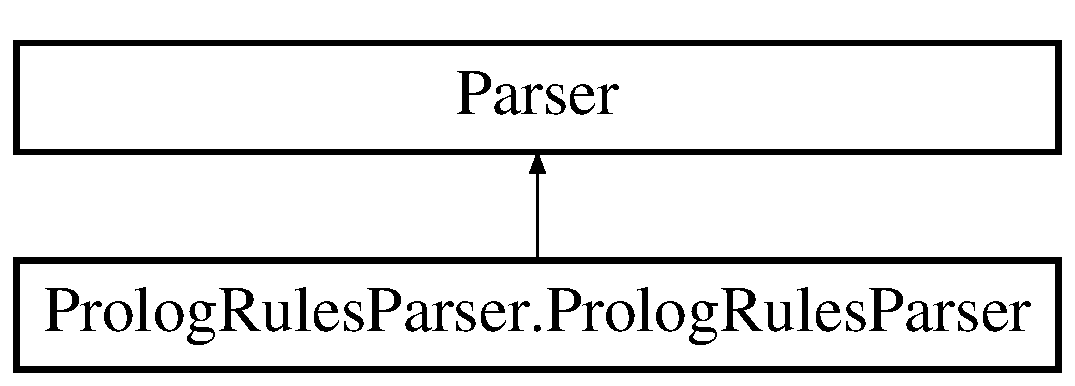
\includegraphics[height=2.000000cm]{class_prolog_rules_parser_1_1_prolog_rules_parser}
\end{center}
\end{figure}
\subsection*{Classes}
\begin{DoxyCompactItemize}
\item 
class \hyperlink{class_prolog_rules_parser_1_1_prolog_rules_parser_1_1_args_context}{Args\+Context}
\item 
class \hyperlink{class_prolog_rules_parser_1_1_prolog_rules_parser_1_1_atom_context}{Atom\+Context}
\item 
class \hyperlink{class_prolog_rules_parser_1_1_prolog_rules_parser_1_1_comparator_context}{Comparator\+Context}
\item 
class \hyperlink{class_prolog_rules_parser_1_1_prolog_rules_parser_1_1_condition_context}{Condition\+Context}
\item 
class \hyperlink{class_prolog_rules_parser_1_1_prolog_rules_parser_1_1_constraint_context}{Constraint\+Context}
\item 
class \hyperlink{class_prolog_rules_parser_1_1_prolog_rules_parser_1_1_fact_context}{Fact\+Context}
\item 
class \hyperlink{class_prolog_rules_parser_1_1_prolog_rules_parser_1_1_guessrule_context}{Guessrule\+Context}
\item 
class \hyperlink{class_prolog_rules_parser_1_1_prolog_rules_parser_1_1_identifier_context}{Identifier\+Context}
\item 
class \hyperlink{class_prolog_rules_parser_1_1_prolog_rules_parser_1_1_mathexpr_context}{Mathexpr\+Context}
\item 
class \hyperlink{class_prolog_rules_parser_1_1_prolog_rules_parser_1_1_negpred_context}{Negpred\+Context}
\item 
class \hyperlink{class_prolog_rules_parser_1_1_prolog_rules_parser_1_1_onearg_context}{Onearg\+Context}
\item 
class \hyperlink{class_prolog_rules_parser_1_1_prolog_rules_parser_1_1_predcount_context}{Predcount\+Context}
\item 
class \hyperlink{class_prolog_rules_parser_1_1_prolog_rules_parser_1_1_predicate_context}{Predicate\+Context}
\item 
class \hyperlink{class_prolog_rules_parser_1_1_prolog_rules_parser_1_1_prologcode_context}{Prologcode\+Context}
\item 
class \hyperlink{class_prolog_rules_parser_1_1_prolog_rules_parser_1_1_prologrule_context}{Prologrule\+Context}
\item 
class \hyperlink{class_prolog_rules_parser_1_1_prolog_rules_parser_1_1_prologthing_context}{Prologthing\+Context}
\item 
class \hyperlink{class_prolog_rules_parser_1_1_prolog_rules_parser_1_1_rulebody_context}{Rulebody\+Context}
\item 
class \hyperlink{class_prolog_rules_parser_1_1_prolog_rules_parser_1_1_somerule_context}{Somerule\+Context}
\end{DoxyCompactItemize}
\subsection*{Public Member Functions}
\begin{DoxyCompactItemize}
\item 
def \hyperlink{class_prolog_rules_parser_1_1_prolog_rules_parser_a5b5dedde829a4a6dc45c225465d3f51c}{\+\_\+\+\_\+init\+\_\+\+\_\+} (self, input)
\item 
def \hyperlink{class_prolog_rules_parser_1_1_prolog_rules_parser_ad1add6bc3c38625422bb746b40ba9dcc}{prologcode} (self)
\item 
def \hyperlink{class_prolog_rules_parser_1_1_prolog_rules_parser_a2882956c0c420c8508faeaca6bab3dee}{prologthing} (self)
\item 
def \hyperlink{class_prolog_rules_parser_1_1_prolog_rules_parser_ad6573773c7353080cc4423fefa2bf9c1}{fact} (self)
\item 
def \hyperlink{class_prolog_rules_parser_1_1_prolog_rules_parser_a619f24dbdfc7ec8a030f971789303611}{constraint} (self)
\item 
def \hyperlink{class_prolog_rules_parser_1_1_prolog_rules_parser_a1c80a3ef38bae5f3b1307bb4c23cd21a}{somerule} (self)
\item 
def \hyperlink{class_prolog_rules_parser_1_1_prolog_rules_parser_ad25635a83fec128ac019ba9e834ccd62}{prologrule} (self)
\item 
def \hyperlink{class_prolog_rules_parser_1_1_prolog_rules_parser_ab5d0165c626fa325700f2b9440ff5f95}{guessrule} (self)
\item 
def \hyperlink{class_prolog_rules_parser_1_1_prolog_rules_parser_a584d4ae09186dc19ae884b311f717c8d}{predcount} (self)
\item 
def \hyperlink{class_prolog_rules_parser_1_1_prolog_rules_parser_a3596b1ef3edd927166ea998f90122e54}{predicate} (self)
\item 
def \hyperlink{class_prolog_rules_parser_1_1_prolog_rules_parser_aaf735595570145e3eacf4d3784e68aa0}{rulebody} (self)
\item 
def \hyperlink{class_prolog_rules_parser_1_1_prolog_rules_parser_ac0b44714c95679b75feb5b4ef2f2ce48}{condition} (self)
\item 
def \hyperlink{class_prolog_rules_parser_1_1_prolog_rules_parser_a298c6fdda53250817c1537170a939091}{negpred} (self)
\item 
def \hyperlink{class_prolog_rules_parser_1_1_prolog_rules_parser_a1796c110404c167f207073d1310be900}{comparator} (self)
\item 
def \hyperlink{class_prolog_rules_parser_1_1_prolog_rules_parser_ac21c5fb3ea30e45c0fefae658a50ad37}{mathexpr} (self)
\item 
def \hyperlink{class_prolog_rules_parser_1_1_prolog_rules_parser_af5d305599be41a95ef7ab92e94967118}{args} (self)
\item 
def \hyperlink{class_prolog_rules_parser_1_1_prolog_rules_parser_a52feaec449cb21dfdb7398e0d610070e}{onearg} (self)
\item 
def \hyperlink{class_prolog_rules_parser_1_1_prolog_rules_parser_a06997778b8bf5a80b797df9773f823d7}{atom} (self)
\item 
def \hyperlink{class_prolog_rules_parser_1_1_prolog_rules_parser_a30e594fbc5e975cd855565d7c6e8170b}{identifier} (self)
\end{DoxyCompactItemize}
\subsection*{Public Attributes}
\begin{DoxyCompactItemize}
\item 
\hyperlink{class_prolog_rules_parser_1_1_prolog_rules_parser_a250a340ccf9e9fcefe5b2e8b4197385f}{state}
\end{DoxyCompactItemize}
\subsection*{Static Public Attributes}
\begin{DoxyCompactItemize}
\item 
string \hyperlink{class_prolog_rules_parser_1_1_prolog_rules_parser_a15377f7b025a77756d36114c83a91004}{grammar\+File\+Name} = \char`\"{}java-\/escape\char`\"{}
\item 
tuple \hyperlink{class_prolog_rules_parser_1_1_prolog_rules_parser_af3e5e19ff8bfc25f72bba8323d5b2e4a}{atn} = A\+T\+N\+Deserializer()
\item 
list \hyperlink{class_prolog_rules_parser_1_1_prolog_rules_parser_a61692146dafe00c2cf0d4ab5938c9c68}{decisions\+To\+D\+F\+A} = \mbox{[} D\+F\+A(ds, i) for i, ds in enumerate(atn.\+decision\+To\+State) \mbox{]}
\item 
tuple \hyperlink{class_prolog_rules_parser_1_1_prolog_rules_parser_abcc83c78b7cb5aff6b2cc54f5d33f143}{shared\+Context\+Cache} = Prediction\+Context\+Cache()
\item 
\hyperlink{class_prolog_rules_parser_1_1_prolog_rules_parser_a4b8e8403ff8eb09e1c7b694078f765b2}{E\+O\+F} = Token.\+E\+O\+F
\item 
int \hyperlink{class_prolog_rules_parser_1_1_prolog_rules_parser_a4cb5c955b91ccf5dc36ad6db7202dcce}{T\+\_\+\+\_\+8} = 1
\item 
int \hyperlink{class_prolog_rules_parser_1_1_prolog_rules_parser_a53e7558944feb7cfe1e8bfb1767384ef}{T\+\_\+\+\_\+7} = 2
\item 
int \hyperlink{class_prolog_rules_parser_1_1_prolog_rules_parser_ab1468d401c196881a49f2600042d6d64}{T\+\_\+\+\_\+6} = 3
\item 
int \hyperlink{class_prolog_rules_parser_1_1_prolog_rules_parser_aece390dc6b10828f2a0f04d0d47a8b57}{T\+\_\+\+\_\+5} = 4
\item 
int \hyperlink{class_prolog_rules_parser_1_1_prolog_rules_parser_a844dee3952dd7f26e6b3dcb345e22a91}{T\+\_\+\+\_\+4} = 5
\item 
int \hyperlink{class_prolog_rules_parser_1_1_prolog_rules_parser_a4f48ff3491d8e3fbe7075caf04d8e006}{T\+\_\+\+\_\+3} = 6
\item 
int \hyperlink{class_prolog_rules_parser_1_1_prolog_rules_parser_a2d9aeabd6a653e6300aa32084c9f4983}{T\+\_\+\+\_\+2} = 7
\item 
int \hyperlink{class_prolog_rules_parser_1_1_prolog_rules_parser_ab7ff2effb1ea8358d127c79c272e68c2}{T\+\_\+\+\_\+1} = 8
\item 
int \hyperlink{class_prolog_rules_parser_1_1_prolog_rules_parser_af3c084e99302eea5776f20c1d6ee9a6f}{T\+\_\+\+\_\+0} = 9
\item 
int \hyperlink{class_prolog_rules_parser_1_1_prolog_rules_parser_a2bf01e620d0c3e5dc6cecfcb6e168913}{N\+U\+M\+B\+E\+R} = 10
\item 
int \hyperlink{class_prolog_rules_parser_1_1_prolog_rules_parser_aa289b7878d23e5af994c39d322513c90}{R\+E\+L\+O\+P\+E\+R\+A\+T\+O\+R} = 11
\item 
int \hyperlink{class_prolog_rules_parser_1_1_prolog_rules_parser_a1bb537d25f9ace27b40fa8e537f38f26}{O\+P\+E\+R\+A\+T\+O\+R} = 12
\item 
int \hyperlink{class_prolog_rules_parser_1_1_prolog_rules_parser_a2affda7f9e85561dd655e83074daae42}{W\+O\+R\+D} = 13
\item 
int \hyperlink{class_prolog_rules_parser_1_1_prolog_rules_parser_a6aed4026401dd5ec9cf3db743a976a07}{C\+O\+M\+M\+E\+N\+T} = 14
\item 
int \hyperlink{class_prolog_rules_parser_1_1_prolog_rules_parser_a1c98b9ac6d6a175c852cce914ad6d7ad}{W\+S} = 15
\item 
list \hyperlink{class_prolog_rules_parser_1_1_prolog_rules_parser_a5d992aa2b8f6419f374e365bf76d38d5}{token\+Names}
\item 
int \hyperlink{class_prolog_rules_parser_1_1_prolog_rules_parser_a630f663b0f57488506a6ffc1da9e354a}{R\+U\+L\+E\+\_\+prologcode} = 0
\item 
int \hyperlink{class_prolog_rules_parser_1_1_prolog_rules_parser_a20f16c36ca3e1f291e4777f1c7ed094d}{R\+U\+L\+E\+\_\+prologthing} = 1
\item 
int \hyperlink{class_prolog_rules_parser_1_1_prolog_rules_parser_aba168460a11bb4fed7b3cb91a919c423}{R\+U\+L\+E\+\_\+fact} = 2
\item 
int \hyperlink{class_prolog_rules_parser_1_1_prolog_rules_parser_a38e23788ffd77a44a0de3ccc6bd0eeb5}{R\+U\+L\+E\+\_\+constraint} = 3
\item 
int \hyperlink{class_prolog_rules_parser_1_1_prolog_rules_parser_af40e6329c30ba757f2a1251eb60fd3f3}{R\+U\+L\+E\+\_\+somerule} = 4
\item 
int \hyperlink{class_prolog_rules_parser_1_1_prolog_rules_parser_a619cf8a5fdcf48cfcd417ce3925e848d}{R\+U\+L\+E\+\_\+prologrule} = 5
\item 
int \hyperlink{class_prolog_rules_parser_1_1_prolog_rules_parser_a4d8b7576258fb1f854c4d1d0d8889243}{R\+U\+L\+E\+\_\+guessrule} = 6
\item 
int \hyperlink{class_prolog_rules_parser_1_1_prolog_rules_parser_af5635e81bdacbddb983515a39a661e56}{R\+U\+L\+E\+\_\+predcount} = 7
\item 
int \hyperlink{class_prolog_rules_parser_1_1_prolog_rules_parser_acaa0ad440cba170a8586f0d78a6bf7e2}{R\+U\+L\+E\+\_\+predicate} = 8
\item 
int \hyperlink{class_prolog_rules_parser_1_1_prolog_rules_parser_acd27c1d066aeef36840d89aaaaa79795}{R\+U\+L\+E\+\_\+rulebody} = 9
\item 
int \hyperlink{class_prolog_rules_parser_1_1_prolog_rules_parser_a463b1479e7f7ca4a5b98baad5468647d}{R\+U\+L\+E\+\_\+condition} = 10
\item 
int \hyperlink{class_prolog_rules_parser_1_1_prolog_rules_parser_ae0a9da93cf53d677949708f3ee1eba91}{R\+U\+L\+E\+\_\+negpred} = 11
\item 
int \hyperlink{class_prolog_rules_parser_1_1_prolog_rules_parser_ac54d4c950a548415336043b3dd865d7d}{R\+U\+L\+E\+\_\+comparator} = 12
\item 
int \hyperlink{class_prolog_rules_parser_1_1_prolog_rules_parser_a4d406406107dbe459fb2c3de8cf5e3b8}{R\+U\+L\+E\+\_\+mathexpr} = 13
\item 
int \hyperlink{class_prolog_rules_parser_1_1_prolog_rules_parser_a5280a17312cf9ff3026589fbe178c8c8}{R\+U\+L\+E\+\_\+args} = 14
\item 
int \hyperlink{class_prolog_rules_parser_1_1_prolog_rules_parser_a0d30f19f3b36d3c49b90787774d3124a}{R\+U\+L\+E\+\_\+onearg} = 15
\item 
int \hyperlink{class_prolog_rules_parser_1_1_prolog_rules_parser_a691f884125527c3a3c0c0546d0b9026f}{R\+U\+L\+E\+\_\+atom} = 16
\item 
int \hyperlink{class_prolog_rules_parser_1_1_prolog_rules_parser_a835070742e48135fee80dcece6bc2902}{R\+U\+L\+E\+\_\+identifier} = 17
\item 
list \hyperlink{class_prolog_rules_parser_1_1_prolog_rules_parser_a0faf0fd8785bbe611ec4bc517ca0387a}{rule\+Names}
\end{DoxyCompactItemize}


\subsection{Detailed Description}


Definition at line 71 of file Prolog\+Rules\+Parser.\+py.



\subsection{Constructor \& Destructor Documentation}
\hypertarget{class_prolog_rules_parser_1_1_prolog_rules_parser_a5b5dedde829a4a6dc45c225465d3f51c}{}\index{Prolog\+Rules\+Parser\+::\+Prolog\+Rules\+Parser@{Prolog\+Rules\+Parser\+::\+Prolog\+Rules\+Parser}!\+\_\+\+\_\+init\+\_\+\+\_\+@{\+\_\+\+\_\+init\+\_\+\+\_\+}}
\index{\+\_\+\+\_\+init\+\_\+\+\_\+@{\+\_\+\+\_\+init\+\_\+\+\_\+}!Prolog\+Rules\+Parser\+::\+Prolog\+Rules\+Parser@{Prolog\+Rules\+Parser\+::\+Prolog\+Rules\+Parser}}
\subsubsection[{\+\_\+\+\_\+init\+\_\+\+\_\+}]{\setlength{\rightskip}{0pt plus 5cm}def Prolog\+Rules\+Parser.\+Prolog\+Rules\+Parser.\+\_\+\+\_\+init\+\_\+\+\_\+ (
\begin{DoxyParamCaption}
\item[{}]{self, }
\item[{}]{input}
\end{DoxyParamCaption}
)}\label{class_prolog_rules_parser_1_1_prolog_rules_parser_a5b5dedde829a4a6dc45c225465d3f51c}


Definition at line 127 of file Prolog\+Rules\+Parser.\+py.



\subsection{Member Function Documentation}
\hypertarget{class_prolog_rules_parser_1_1_prolog_rules_parser_af5d305599be41a95ef7ab92e94967118}{}\index{Prolog\+Rules\+Parser\+::\+Prolog\+Rules\+Parser@{Prolog\+Rules\+Parser\+::\+Prolog\+Rules\+Parser}!args@{args}}
\index{args@{args}!Prolog\+Rules\+Parser\+::\+Prolog\+Rules\+Parser@{Prolog\+Rules\+Parser\+::\+Prolog\+Rules\+Parser}}
\subsubsection[{args}]{\setlength{\rightskip}{0pt plus 5cm}def Prolog\+Rules\+Parser.\+Prolog\+Rules\+Parser.\+args (
\begin{DoxyParamCaption}
\item[{}]{self}
\end{DoxyParamCaption}
)}\label{class_prolog_rules_parser_1_1_prolog_rules_parser_af5d305599be41a95ef7ab92e94967118}


Definition at line 1012 of file Prolog\+Rules\+Parser.\+py.

\hypertarget{class_prolog_rules_parser_1_1_prolog_rules_parser_a06997778b8bf5a80b797df9773f823d7}{}\index{Prolog\+Rules\+Parser\+::\+Prolog\+Rules\+Parser@{Prolog\+Rules\+Parser\+::\+Prolog\+Rules\+Parser}!atom@{atom}}
\index{atom@{atom}!Prolog\+Rules\+Parser\+::\+Prolog\+Rules\+Parser@{Prolog\+Rules\+Parser\+::\+Prolog\+Rules\+Parser}}
\subsubsection[{atom}]{\setlength{\rightskip}{0pt plus 5cm}def Prolog\+Rules\+Parser.\+Prolog\+Rules\+Parser.\+atom (
\begin{DoxyParamCaption}
\item[{}]{self}
\end{DoxyParamCaption}
)}\label{class_prolog_rules_parser_1_1_prolog_rules_parser_a06997778b8bf5a80b797df9773f823d7}


Definition at line 1124 of file Prolog\+Rules\+Parser.\+py.

\hypertarget{class_prolog_rules_parser_1_1_prolog_rules_parser_a1796c110404c167f207073d1310be900}{}\index{Prolog\+Rules\+Parser\+::\+Prolog\+Rules\+Parser@{Prolog\+Rules\+Parser\+::\+Prolog\+Rules\+Parser}!comparator@{comparator}}
\index{comparator@{comparator}!Prolog\+Rules\+Parser\+::\+Prolog\+Rules\+Parser@{Prolog\+Rules\+Parser\+::\+Prolog\+Rules\+Parser}}
\subsubsection[{comparator}]{\setlength{\rightskip}{0pt plus 5cm}def Prolog\+Rules\+Parser.\+Prolog\+Rules\+Parser.\+comparator (
\begin{DoxyParamCaption}
\item[{}]{self}
\end{DoxyParamCaption}
)}\label{class_prolog_rules_parser_1_1_prolog_rules_parser_a1796c110404c167f207073d1310be900}


Definition at line 884 of file Prolog\+Rules\+Parser.\+py.

\hypertarget{class_prolog_rules_parser_1_1_prolog_rules_parser_ac0b44714c95679b75feb5b4ef2f2ce48}{}\index{Prolog\+Rules\+Parser\+::\+Prolog\+Rules\+Parser@{Prolog\+Rules\+Parser\+::\+Prolog\+Rules\+Parser}!condition@{condition}}
\index{condition@{condition}!Prolog\+Rules\+Parser\+::\+Prolog\+Rules\+Parser@{Prolog\+Rules\+Parser\+::\+Prolog\+Rules\+Parser}}
\subsubsection[{condition}]{\setlength{\rightskip}{0pt plus 5cm}def Prolog\+Rules\+Parser.\+Prolog\+Rules\+Parser.\+condition (
\begin{DoxyParamCaption}
\item[{}]{self}
\end{DoxyParamCaption}
)}\label{class_prolog_rules_parser_1_1_prolog_rules_parser_ac0b44714c95679b75feb5b4ef2f2ce48}


Definition at line 771 of file Prolog\+Rules\+Parser.\+py.

\hypertarget{class_prolog_rules_parser_1_1_prolog_rules_parser_a619f24dbdfc7ec8a030f971789303611}{}\index{Prolog\+Rules\+Parser\+::\+Prolog\+Rules\+Parser@{Prolog\+Rules\+Parser\+::\+Prolog\+Rules\+Parser}!constraint@{constraint}}
\index{constraint@{constraint}!Prolog\+Rules\+Parser\+::\+Prolog\+Rules\+Parser@{Prolog\+Rules\+Parser\+::\+Prolog\+Rules\+Parser}}
\subsubsection[{constraint}]{\setlength{\rightskip}{0pt plus 5cm}def Prolog\+Rules\+Parser.\+Prolog\+Rules\+Parser.\+constraint (
\begin{DoxyParamCaption}
\item[{}]{self}
\end{DoxyParamCaption}
)}\label{class_prolog_rules_parser_1_1_prolog_rules_parser_a619f24dbdfc7ec8a030f971789303611}


Definition at line 321 of file Prolog\+Rules\+Parser.\+py.

\hypertarget{class_prolog_rules_parser_1_1_prolog_rules_parser_ad6573773c7353080cc4423fefa2bf9c1}{}\index{Prolog\+Rules\+Parser\+::\+Prolog\+Rules\+Parser@{Prolog\+Rules\+Parser\+::\+Prolog\+Rules\+Parser}!fact@{fact}}
\index{fact@{fact}!Prolog\+Rules\+Parser\+::\+Prolog\+Rules\+Parser@{Prolog\+Rules\+Parser\+::\+Prolog\+Rules\+Parser}}
\subsubsection[{fact}]{\setlength{\rightskip}{0pt plus 5cm}def Prolog\+Rules\+Parser.\+Prolog\+Rules\+Parser.\+fact (
\begin{DoxyParamCaption}
\item[{}]{self}
\end{DoxyParamCaption}
)}\label{class_prolog_rules_parser_1_1_prolog_rules_parser_ad6573773c7353080cc4423fefa2bf9c1}


Definition at line 279 of file Prolog\+Rules\+Parser.\+py.

\hypertarget{class_prolog_rules_parser_1_1_prolog_rules_parser_ab5d0165c626fa325700f2b9440ff5f95}{}\index{Prolog\+Rules\+Parser\+::\+Prolog\+Rules\+Parser@{Prolog\+Rules\+Parser\+::\+Prolog\+Rules\+Parser}!guessrule@{guessrule}}
\index{guessrule@{guessrule}!Prolog\+Rules\+Parser\+::\+Prolog\+Rules\+Parser@{Prolog\+Rules\+Parser\+::\+Prolog\+Rules\+Parser}}
\subsubsection[{guessrule}]{\setlength{\rightskip}{0pt plus 5cm}def Prolog\+Rules\+Parser.\+Prolog\+Rules\+Parser.\+guessrule (
\begin{DoxyParamCaption}
\item[{}]{self}
\end{DoxyParamCaption}
)}\label{class_prolog_rules_parser_1_1_prolog_rules_parser_ab5d0165c626fa325700f2b9440ff5f95}


Definition at line 484 of file Prolog\+Rules\+Parser.\+py.

\hypertarget{class_prolog_rules_parser_1_1_prolog_rules_parser_a30e594fbc5e975cd855565d7c6e8170b}{}\index{Prolog\+Rules\+Parser\+::\+Prolog\+Rules\+Parser@{Prolog\+Rules\+Parser\+::\+Prolog\+Rules\+Parser}!identifier@{identifier}}
\index{identifier@{identifier}!Prolog\+Rules\+Parser\+::\+Prolog\+Rules\+Parser@{Prolog\+Rules\+Parser\+::\+Prolog\+Rules\+Parser}}
\subsubsection[{identifier}]{\setlength{\rightskip}{0pt plus 5cm}def Prolog\+Rules\+Parser.\+Prolog\+Rules\+Parser.\+identifier (
\begin{DoxyParamCaption}
\item[{}]{self}
\end{DoxyParamCaption}
)}\label{class_prolog_rules_parser_1_1_prolog_rules_parser_a30e594fbc5e975cd855565d7c6e8170b}


Definition at line 1175 of file Prolog\+Rules\+Parser.\+py.

\hypertarget{class_prolog_rules_parser_1_1_prolog_rules_parser_ac21c5fb3ea30e45c0fefae658a50ad37}{}\index{Prolog\+Rules\+Parser\+::\+Prolog\+Rules\+Parser@{Prolog\+Rules\+Parser\+::\+Prolog\+Rules\+Parser}!mathexpr@{mathexpr}}
\index{mathexpr@{mathexpr}!Prolog\+Rules\+Parser\+::\+Prolog\+Rules\+Parser@{Prolog\+Rules\+Parser\+::\+Prolog\+Rules\+Parser}}
\subsubsection[{mathexpr}]{\setlength{\rightskip}{0pt plus 5cm}def Prolog\+Rules\+Parser.\+Prolog\+Rules\+Parser.\+mathexpr (
\begin{DoxyParamCaption}
\item[{}]{self}
\end{DoxyParamCaption}
)}\label{class_prolog_rules_parser_1_1_prolog_rules_parser_ac21c5fb3ea30e45c0fefae658a50ad37}


Definition at line 939 of file Prolog\+Rules\+Parser.\+py.

\hypertarget{class_prolog_rules_parser_1_1_prolog_rules_parser_a298c6fdda53250817c1537170a939091}{}\index{Prolog\+Rules\+Parser\+::\+Prolog\+Rules\+Parser@{Prolog\+Rules\+Parser\+::\+Prolog\+Rules\+Parser}!negpred@{negpred}}
\index{negpred@{negpred}!Prolog\+Rules\+Parser\+::\+Prolog\+Rules\+Parser@{Prolog\+Rules\+Parser\+::\+Prolog\+Rules\+Parser}}
\subsubsection[{negpred}]{\setlength{\rightskip}{0pt plus 5cm}def Prolog\+Rules\+Parser.\+Prolog\+Rules\+Parser.\+negpred (
\begin{DoxyParamCaption}
\item[{}]{self}
\end{DoxyParamCaption}
)}\label{class_prolog_rules_parser_1_1_prolog_rules_parser_a298c6fdda53250817c1537170a939091}


Definition at line 835 of file Prolog\+Rules\+Parser.\+py.

\hypertarget{class_prolog_rules_parser_1_1_prolog_rules_parser_a52feaec449cb21dfdb7398e0d610070e}{}\index{Prolog\+Rules\+Parser\+::\+Prolog\+Rules\+Parser@{Prolog\+Rules\+Parser\+::\+Prolog\+Rules\+Parser}!onearg@{onearg}}
\index{onearg@{onearg}!Prolog\+Rules\+Parser\+::\+Prolog\+Rules\+Parser@{Prolog\+Rules\+Parser\+::\+Prolog\+Rules\+Parser}}
\subsubsection[{onearg}]{\setlength{\rightskip}{0pt plus 5cm}def Prolog\+Rules\+Parser.\+Prolog\+Rules\+Parser.\+onearg (
\begin{DoxyParamCaption}
\item[{}]{self}
\end{DoxyParamCaption}
)}\label{class_prolog_rules_parser_1_1_prolog_rules_parser_a52feaec449cb21dfdb7398e0d610070e}


Definition at line 1069 of file Prolog\+Rules\+Parser.\+py.

\hypertarget{class_prolog_rules_parser_1_1_prolog_rules_parser_a584d4ae09186dc19ae884b311f717c8d}{}\index{Prolog\+Rules\+Parser\+::\+Prolog\+Rules\+Parser@{Prolog\+Rules\+Parser\+::\+Prolog\+Rules\+Parser}!predcount@{predcount}}
\index{predcount@{predcount}!Prolog\+Rules\+Parser\+::\+Prolog\+Rules\+Parser@{Prolog\+Rules\+Parser\+::\+Prolog\+Rules\+Parser}}
\subsubsection[{predcount}]{\setlength{\rightskip}{0pt plus 5cm}def Prolog\+Rules\+Parser.\+Prolog\+Rules\+Parser.\+predcount (
\begin{DoxyParamCaption}
\item[{}]{self}
\end{DoxyParamCaption}
)}\label{class_prolog_rules_parser_1_1_prolog_rules_parser_a584d4ae09186dc19ae884b311f717c8d}


Definition at line 569 of file Prolog\+Rules\+Parser.\+py.

\hypertarget{class_prolog_rules_parser_1_1_prolog_rules_parser_a3596b1ef3edd927166ea998f90122e54}{}\index{Prolog\+Rules\+Parser\+::\+Prolog\+Rules\+Parser@{Prolog\+Rules\+Parser\+::\+Prolog\+Rules\+Parser}!predicate@{predicate}}
\index{predicate@{predicate}!Prolog\+Rules\+Parser\+::\+Prolog\+Rules\+Parser@{Prolog\+Rules\+Parser\+::\+Prolog\+Rules\+Parser}}
\subsubsection[{predicate}]{\setlength{\rightskip}{0pt plus 5cm}def Prolog\+Rules\+Parser.\+Prolog\+Rules\+Parser.\+predicate (
\begin{DoxyParamCaption}
\item[{}]{self}
\end{DoxyParamCaption}
)}\label{class_prolog_rules_parser_1_1_prolog_rules_parser_a3596b1ef3edd927166ea998f90122e54}


Definition at line 641 of file Prolog\+Rules\+Parser.\+py.

\hypertarget{class_prolog_rules_parser_1_1_prolog_rules_parser_ad1add6bc3c38625422bb746b40ba9dcc}{}\index{Prolog\+Rules\+Parser\+::\+Prolog\+Rules\+Parser@{Prolog\+Rules\+Parser\+::\+Prolog\+Rules\+Parser}!prologcode@{prologcode}}
\index{prologcode@{prologcode}!Prolog\+Rules\+Parser\+::\+Prolog\+Rules\+Parser@{Prolog\+Rules\+Parser\+::\+Prolog\+Rules\+Parser}}
\subsubsection[{prologcode}]{\setlength{\rightskip}{0pt plus 5cm}def Prolog\+Rules\+Parser.\+Prolog\+Rules\+Parser.\+prologcode (
\begin{DoxyParamCaption}
\item[{}]{self}
\end{DoxyParamCaption}
)}\label{class_prolog_rules_parser_1_1_prolog_rules_parser_ad1add6bc3c38625422bb746b40ba9dcc}


Definition at line 162 of file Prolog\+Rules\+Parser.\+py.

\hypertarget{class_prolog_rules_parser_1_1_prolog_rules_parser_ad25635a83fec128ac019ba9e834ccd62}{}\index{Prolog\+Rules\+Parser\+::\+Prolog\+Rules\+Parser@{Prolog\+Rules\+Parser\+::\+Prolog\+Rules\+Parser}!prologrule@{prologrule}}
\index{prologrule@{prologrule}!Prolog\+Rules\+Parser\+::\+Prolog\+Rules\+Parser@{Prolog\+Rules\+Parser\+::\+Prolog\+Rules\+Parser}}
\subsubsection[{prologrule}]{\setlength{\rightskip}{0pt plus 5cm}def Prolog\+Rules\+Parser.\+Prolog\+Rules\+Parser.\+prologrule (
\begin{DoxyParamCaption}
\item[{}]{self}
\end{DoxyParamCaption}
)}\label{class_prolog_rules_parser_1_1_prolog_rules_parser_ad25635a83fec128ac019ba9e834ccd62}


Definition at line 425 of file Prolog\+Rules\+Parser.\+py.

\hypertarget{class_prolog_rules_parser_1_1_prolog_rules_parser_a2882956c0c420c8508faeaca6bab3dee}{}\index{Prolog\+Rules\+Parser\+::\+Prolog\+Rules\+Parser@{Prolog\+Rules\+Parser\+::\+Prolog\+Rules\+Parser}!prologthing@{prologthing}}
\index{prologthing@{prologthing}!Prolog\+Rules\+Parser\+::\+Prolog\+Rules\+Parser@{Prolog\+Rules\+Parser\+::\+Prolog\+Rules\+Parser}}
\subsubsection[{prologthing}]{\setlength{\rightskip}{0pt plus 5cm}def Prolog\+Rules\+Parser.\+Prolog\+Rules\+Parser.\+prologthing (
\begin{DoxyParamCaption}
\item[{}]{self}
\end{DoxyParamCaption}
)}\label{class_prolog_rules_parser_1_1_prolog_rules_parser_a2882956c0c420c8508faeaca6bab3dee}


Definition at line 221 of file Prolog\+Rules\+Parser.\+py.

\hypertarget{class_prolog_rules_parser_1_1_prolog_rules_parser_aaf735595570145e3eacf4d3784e68aa0}{}\index{Prolog\+Rules\+Parser\+::\+Prolog\+Rules\+Parser@{Prolog\+Rules\+Parser\+::\+Prolog\+Rules\+Parser}!rulebody@{rulebody}}
\index{rulebody@{rulebody}!Prolog\+Rules\+Parser\+::\+Prolog\+Rules\+Parser@{Prolog\+Rules\+Parser\+::\+Prolog\+Rules\+Parser}}
\subsubsection[{rulebody}]{\setlength{\rightskip}{0pt plus 5cm}def Prolog\+Rules\+Parser.\+Prolog\+Rules\+Parser.\+rulebody (
\begin{DoxyParamCaption}
\item[{}]{self}
\end{DoxyParamCaption}
)}\label{class_prolog_rules_parser_1_1_prolog_rules_parser_aaf735595570145e3eacf4d3784e68aa0}


Definition at line 703 of file Prolog\+Rules\+Parser.\+py.

\hypertarget{class_prolog_rules_parser_1_1_prolog_rules_parser_a1c80a3ef38bae5f3b1307bb4c23cd21a}{}\index{Prolog\+Rules\+Parser\+::\+Prolog\+Rules\+Parser@{Prolog\+Rules\+Parser\+::\+Prolog\+Rules\+Parser}!somerule@{somerule}}
\index{somerule@{somerule}!Prolog\+Rules\+Parser\+::\+Prolog\+Rules\+Parser@{Prolog\+Rules\+Parser\+::\+Prolog\+Rules\+Parser}}
\subsubsection[{somerule}]{\setlength{\rightskip}{0pt plus 5cm}def Prolog\+Rules\+Parser.\+Prolog\+Rules\+Parser.\+somerule (
\begin{DoxyParamCaption}
\item[{}]{self}
\end{DoxyParamCaption}
)}\label{class_prolog_rules_parser_1_1_prolog_rules_parser_a1c80a3ef38bae5f3b1307bb4c23cd21a}


Definition at line 369 of file Prolog\+Rules\+Parser.\+py.



\subsection{Member Data Documentation}
\hypertarget{class_prolog_rules_parser_1_1_prolog_rules_parser_af3e5e19ff8bfc25f72bba8323d5b2e4a}{}\index{Prolog\+Rules\+Parser\+::\+Prolog\+Rules\+Parser@{Prolog\+Rules\+Parser\+::\+Prolog\+Rules\+Parser}!atn@{atn}}
\index{atn@{atn}!Prolog\+Rules\+Parser\+::\+Prolog\+Rules\+Parser@{Prolog\+Rules\+Parser\+::\+Prolog\+Rules\+Parser}}
\subsubsection[{atn}]{\setlength{\rightskip}{0pt plus 5cm}tuple Prolog\+Rules\+Parser.\+Prolog\+Rules\+Parser.\+atn = A\+T\+N\+Deserializer()\hspace{0.3cm}{\ttfamily [static]}}\label{class_prolog_rules_parser_1_1_prolog_rules_parser_af3e5e19ff8bfc25f72bba8323d5b2e4a}


Definition at line 75 of file Prolog\+Rules\+Parser.\+py.

\hypertarget{class_prolog_rules_parser_1_1_prolog_rules_parser_a6aed4026401dd5ec9cf3db743a976a07}{}\index{Prolog\+Rules\+Parser\+::\+Prolog\+Rules\+Parser@{Prolog\+Rules\+Parser\+::\+Prolog\+Rules\+Parser}!C\+O\+M\+M\+E\+N\+T@{C\+O\+M\+M\+E\+N\+T}}
\index{C\+O\+M\+M\+E\+N\+T@{C\+O\+M\+M\+E\+N\+T}!Prolog\+Rules\+Parser\+::\+Prolog\+Rules\+Parser@{Prolog\+Rules\+Parser\+::\+Prolog\+Rules\+Parser}}
\subsubsection[{C\+O\+M\+M\+E\+N\+T}]{\setlength{\rightskip}{0pt plus 5cm}int Prolog\+Rules\+Parser.\+Prolog\+Rules\+Parser.\+C\+O\+M\+M\+E\+N\+T = 14\hspace{0.3cm}{\ttfamily [static]}}\label{class_prolog_rules_parser_1_1_prolog_rules_parser_a6aed4026401dd5ec9cf3db743a976a07}


Definition at line 95 of file Prolog\+Rules\+Parser.\+py.

\hypertarget{class_prolog_rules_parser_1_1_prolog_rules_parser_a61692146dafe00c2cf0d4ab5938c9c68}{}\index{Prolog\+Rules\+Parser\+::\+Prolog\+Rules\+Parser@{Prolog\+Rules\+Parser\+::\+Prolog\+Rules\+Parser}!decisions\+To\+D\+F\+A@{decisions\+To\+D\+F\+A}}
\index{decisions\+To\+D\+F\+A@{decisions\+To\+D\+F\+A}!Prolog\+Rules\+Parser\+::\+Prolog\+Rules\+Parser@{Prolog\+Rules\+Parser\+::\+Prolog\+Rules\+Parser}}
\subsubsection[{decisions\+To\+D\+F\+A}]{\setlength{\rightskip}{0pt plus 5cm}list Prolog\+Rules\+Parser.\+Prolog\+Rules\+Parser.\+decisions\+To\+D\+F\+A = \mbox{[} D\+F\+A(ds, i) for i, ds in enumerate(atn.\+decision\+To\+State) \mbox{]}\hspace{0.3cm}{\ttfamily [static]}}\label{class_prolog_rules_parser_1_1_prolog_rules_parser_a61692146dafe00c2cf0d4ab5938c9c68}


Definition at line 77 of file Prolog\+Rules\+Parser.\+py.

\hypertarget{class_prolog_rules_parser_1_1_prolog_rules_parser_a4b8e8403ff8eb09e1c7b694078f765b2}{}\index{Prolog\+Rules\+Parser\+::\+Prolog\+Rules\+Parser@{Prolog\+Rules\+Parser\+::\+Prolog\+Rules\+Parser}!E\+O\+F@{E\+O\+F}}
\index{E\+O\+F@{E\+O\+F}!Prolog\+Rules\+Parser\+::\+Prolog\+Rules\+Parser@{Prolog\+Rules\+Parser\+::\+Prolog\+Rules\+Parser}}
\subsubsection[{E\+O\+F}]{\setlength{\rightskip}{0pt plus 5cm}Prolog\+Rules\+Parser.\+Prolog\+Rules\+Parser.\+E\+O\+F = Token.\+E\+O\+F\hspace{0.3cm}{\ttfamily [static]}}\label{class_prolog_rules_parser_1_1_prolog_rules_parser_a4b8e8403ff8eb09e1c7b694078f765b2}


Definition at line 81 of file Prolog\+Rules\+Parser.\+py.

\hypertarget{class_prolog_rules_parser_1_1_prolog_rules_parser_a15377f7b025a77756d36114c83a91004}{}\index{Prolog\+Rules\+Parser\+::\+Prolog\+Rules\+Parser@{Prolog\+Rules\+Parser\+::\+Prolog\+Rules\+Parser}!grammar\+File\+Name@{grammar\+File\+Name}}
\index{grammar\+File\+Name@{grammar\+File\+Name}!Prolog\+Rules\+Parser\+::\+Prolog\+Rules\+Parser@{Prolog\+Rules\+Parser\+::\+Prolog\+Rules\+Parser}}
\subsubsection[{grammar\+File\+Name}]{\setlength{\rightskip}{0pt plus 5cm}string Prolog\+Rules\+Parser.\+Prolog\+Rules\+Parser.\+grammar\+File\+Name = \char`\"{}java-\/escape\char`\"{}\hspace{0.3cm}{\ttfamily [static]}}\label{class_prolog_rules_parser_1_1_prolog_rules_parser_a15377f7b025a77756d36114c83a91004}


Definition at line 73 of file Prolog\+Rules\+Parser.\+py.

\hypertarget{class_prolog_rules_parser_1_1_prolog_rules_parser_a2bf01e620d0c3e5dc6cecfcb6e168913}{}\index{Prolog\+Rules\+Parser\+::\+Prolog\+Rules\+Parser@{Prolog\+Rules\+Parser\+::\+Prolog\+Rules\+Parser}!N\+U\+M\+B\+E\+R@{N\+U\+M\+B\+E\+R}}
\index{N\+U\+M\+B\+E\+R@{N\+U\+M\+B\+E\+R}!Prolog\+Rules\+Parser\+::\+Prolog\+Rules\+Parser@{Prolog\+Rules\+Parser\+::\+Prolog\+Rules\+Parser}}
\subsubsection[{N\+U\+M\+B\+E\+R}]{\setlength{\rightskip}{0pt plus 5cm}int Prolog\+Rules\+Parser.\+Prolog\+Rules\+Parser.\+N\+U\+M\+B\+E\+R = 10\hspace{0.3cm}{\ttfamily [static]}}\label{class_prolog_rules_parser_1_1_prolog_rules_parser_a2bf01e620d0c3e5dc6cecfcb6e168913}


Definition at line 91 of file Prolog\+Rules\+Parser.\+py.

\hypertarget{class_prolog_rules_parser_1_1_prolog_rules_parser_a1bb537d25f9ace27b40fa8e537f38f26}{}\index{Prolog\+Rules\+Parser\+::\+Prolog\+Rules\+Parser@{Prolog\+Rules\+Parser\+::\+Prolog\+Rules\+Parser}!O\+P\+E\+R\+A\+T\+O\+R@{O\+P\+E\+R\+A\+T\+O\+R}}
\index{O\+P\+E\+R\+A\+T\+O\+R@{O\+P\+E\+R\+A\+T\+O\+R}!Prolog\+Rules\+Parser\+::\+Prolog\+Rules\+Parser@{Prolog\+Rules\+Parser\+::\+Prolog\+Rules\+Parser}}
\subsubsection[{O\+P\+E\+R\+A\+T\+O\+R}]{\setlength{\rightskip}{0pt plus 5cm}int Prolog\+Rules\+Parser.\+Prolog\+Rules\+Parser.\+O\+P\+E\+R\+A\+T\+O\+R = 12\hspace{0.3cm}{\ttfamily [static]}}\label{class_prolog_rules_parser_1_1_prolog_rules_parser_a1bb537d25f9ace27b40fa8e537f38f26}


Definition at line 93 of file Prolog\+Rules\+Parser.\+py.

\hypertarget{class_prolog_rules_parser_1_1_prolog_rules_parser_aa289b7878d23e5af994c39d322513c90}{}\index{Prolog\+Rules\+Parser\+::\+Prolog\+Rules\+Parser@{Prolog\+Rules\+Parser\+::\+Prolog\+Rules\+Parser}!R\+E\+L\+O\+P\+E\+R\+A\+T\+O\+R@{R\+E\+L\+O\+P\+E\+R\+A\+T\+O\+R}}
\index{R\+E\+L\+O\+P\+E\+R\+A\+T\+O\+R@{R\+E\+L\+O\+P\+E\+R\+A\+T\+O\+R}!Prolog\+Rules\+Parser\+::\+Prolog\+Rules\+Parser@{Prolog\+Rules\+Parser\+::\+Prolog\+Rules\+Parser}}
\subsubsection[{R\+E\+L\+O\+P\+E\+R\+A\+T\+O\+R}]{\setlength{\rightskip}{0pt plus 5cm}int Prolog\+Rules\+Parser.\+Prolog\+Rules\+Parser.\+R\+E\+L\+O\+P\+E\+R\+A\+T\+O\+R = 11\hspace{0.3cm}{\ttfamily [static]}}\label{class_prolog_rules_parser_1_1_prolog_rules_parser_aa289b7878d23e5af994c39d322513c90}


Definition at line 92 of file Prolog\+Rules\+Parser.\+py.

\hypertarget{class_prolog_rules_parser_1_1_prolog_rules_parser_a5280a17312cf9ff3026589fbe178c8c8}{}\index{Prolog\+Rules\+Parser\+::\+Prolog\+Rules\+Parser@{Prolog\+Rules\+Parser\+::\+Prolog\+Rules\+Parser}!R\+U\+L\+E\+\_\+args@{R\+U\+L\+E\+\_\+args}}
\index{R\+U\+L\+E\+\_\+args@{R\+U\+L\+E\+\_\+args}!Prolog\+Rules\+Parser\+::\+Prolog\+Rules\+Parser@{Prolog\+Rules\+Parser\+::\+Prolog\+Rules\+Parser}}
\subsubsection[{R\+U\+L\+E\+\_\+args}]{\setlength{\rightskip}{0pt plus 5cm}int Prolog\+Rules\+Parser.\+Prolog\+Rules\+Parser.\+R\+U\+L\+E\+\_\+args = 14\hspace{0.3cm}{\ttfamily [static]}}\label{class_prolog_rules_parser_1_1_prolog_rules_parser_a5280a17312cf9ff3026589fbe178c8c8}


Definition at line 116 of file Prolog\+Rules\+Parser.\+py.

\hypertarget{class_prolog_rules_parser_1_1_prolog_rules_parser_a691f884125527c3a3c0c0546d0b9026f}{}\index{Prolog\+Rules\+Parser\+::\+Prolog\+Rules\+Parser@{Prolog\+Rules\+Parser\+::\+Prolog\+Rules\+Parser}!R\+U\+L\+E\+\_\+atom@{R\+U\+L\+E\+\_\+atom}}
\index{R\+U\+L\+E\+\_\+atom@{R\+U\+L\+E\+\_\+atom}!Prolog\+Rules\+Parser\+::\+Prolog\+Rules\+Parser@{Prolog\+Rules\+Parser\+::\+Prolog\+Rules\+Parser}}
\subsubsection[{R\+U\+L\+E\+\_\+atom}]{\setlength{\rightskip}{0pt plus 5cm}int Prolog\+Rules\+Parser.\+Prolog\+Rules\+Parser.\+R\+U\+L\+E\+\_\+atom = 16\hspace{0.3cm}{\ttfamily [static]}}\label{class_prolog_rules_parser_1_1_prolog_rules_parser_a691f884125527c3a3c0c0546d0b9026f}


Definition at line 118 of file Prolog\+Rules\+Parser.\+py.

\hypertarget{class_prolog_rules_parser_1_1_prolog_rules_parser_ac54d4c950a548415336043b3dd865d7d}{}\index{Prolog\+Rules\+Parser\+::\+Prolog\+Rules\+Parser@{Prolog\+Rules\+Parser\+::\+Prolog\+Rules\+Parser}!R\+U\+L\+E\+\_\+comparator@{R\+U\+L\+E\+\_\+comparator}}
\index{R\+U\+L\+E\+\_\+comparator@{R\+U\+L\+E\+\_\+comparator}!Prolog\+Rules\+Parser\+::\+Prolog\+Rules\+Parser@{Prolog\+Rules\+Parser\+::\+Prolog\+Rules\+Parser}}
\subsubsection[{R\+U\+L\+E\+\_\+comparator}]{\setlength{\rightskip}{0pt plus 5cm}int Prolog\+Rules\+Parser.\+Prolog\+Rules\+Parser.\+R\+U\+L\+E\+\_\+comparator = 12\hspace{0.3cm}{\ttfamily [static]}}\label{class_prolog_rules_parser_1_1_prolog_rules_parser_ac54d4c950a548415336043b3dd865d7d}


Definition at line 114 of file Prolog\+Rules\+Parser.\+py.

\hypertarget{class_prolog_rules_parser_1_1_prolog_rules_parser_a463b1479e7f7ca4a5b98baad5468647d}{}\index{Prolog\+Rules\+Parser\+::\+Prolog\+Rules\+Parser@{Prolog\+Rules\+Parser\+::\+Prolog\+Rules\+Parser}!R\+U\+L\+E\+\_\+condition@{R\+U\+L\+E\+\_\+condition}}
\index{R\+U\+L\+E\+\_\+condition@{R\+U\+L\+E\+\_\+condition}!Prolog\+Rules\+Parser\+::\+Prolog\+Rules\+Parser@{Prolog\+Rules\+Parser\+::\+Prolog\+Rules\+Parser}}
\subsubsection[{R\+U\+L\+E\+\_\+condition}]{\setlength{\rightskip}{0pt plus 5cm}int Prolog\+Rules\+Parser.\+Prolog\+Rules\+Parser.\+R\+U\+L\+E\+\_\+condition = 10\hspace{0.3cm}{\ttfamily [static]}}\label{class_prolog_rules_parser_1_1_prolog_rules_parser_a463b1479e7f7ca4a5b98baad5468647d}


Definition at line 112 of file Prolog\+Rules\+Parser.\+py.

\hypertarget{class_prolog_rules_parser_1_1_prolog_rules_parser_a38e23788ffd77a44a0de3ccc6bd0eeb5}{}\index{Prolog\+Rules\+Parser\+::\+Prolog\+Rules\+Parser@{Prolog\+Rules\+Parser\+::\+Prolog\+Rules\+Parser}!R\+U\+L\+E\+\_\+constraint@{R\+U\+L\+E\+\_\+constraint}}
\index{R\+U\+L\+E\+\_\+constraint@{R\+U\+L\+E\+\_\+constraint}!Prolog\+Rules\+Parser\+::\+Prolog\+Rules\+Parser@{Prolog\+Rules\+Parser\+::\+Prolog\+Rules\+Parser}}
\subsubsection[{R\+U\+L\+E\+\_\+constraint}]{\setlength{\rightskip}{0pt plus 5cm}int Prolog\+Rules\+Parser.\+Prolog\+Rules\+Parser.\+R\+U\+L\+E\+\_\+constraint = 3\hspace{0.3cm}{\ttfamily [static]}}\label{class_prolog_rules_parser_1_1_prolog_rules_parser_a38e23788ffd77a44a0de3ccc6bd0eeb5}


Definition at line 105 of file Prolog\+Rules\+Parser.\+py.

\hypertarget{class_prolog_rules_parser_1_1_prolog_rules_parser_aba168460a11bb4fed7b3cb91a919c423}{}\index{Prolog\+Rules\+Parser\+::\+Prolog\+Rules\+Parser@{Prolog\+Rules\+Parser\+::\+Prolog\+Rules\+Parser}!R\+U\+L\+E\+\_\+fact@{R\+U\+L\+E\+\_\+fact}}
\index{R\+U\+L\+E\+\_\+fact@{R\+U\+L\+E\+\_\+fact}!Prolog\+Rules\+Parser\+::\+Prolog\+Rules\+Parser@{Prolog\+Rules\+Parser\+::\+Prolog\+Rules\+Parser}}
\subsubsection[{R\+U\+L\+E\+\_\+fact}]{\setlength{\rightskip}{0pt plus 5cm}int Prolog\+Rules\+Parser.\+Prolog\+Rules\+Parser.\+R\+U\+L\+E\+\_\+fact = 2\hspace{0.3cm}{\ttfamily [static]}}\label{class_prolog_rules_parser_1_1_prolog_rules_parser_aba168460a11bb4fed7b3cb91a919c423}


Definition at line 104 of file Prolog\+Rules\+Parser.\+py.

\hypertarget{class_prolog_rules_parser_1_1_prolog_rules_parser_a4d8b7576258fb1f854c4d1d0d8889243}{}\index{Prolog\+Rules\+Parser\+::\+Prolog\+Rules\+Parser@{Prolog\+Rules\+Parser\+::\+Prolog\+Rules\+Parser}!R\+U\+L\+E\+\_\+guessrule@{R\+U\+L\+E\+\_\+guessrule}}
\index{R\+U\+L\+E\+\_\+guessrule@{R\+U\+L\+E\+\_\+guessrule}!Prolog\+Rules\+Parser\+::\+Prolog\+Rules\+Parser@{Prolog\+Rules\+Parser\+::\+Prolog\+Rules\+Parser}}
\subsubsection[{R\+U\+L\+E\+\_\+guessrule}]{\setlength{\rightskip}{0pt plus 5cm}int Prolog\+Rules\+Parser.\+Prolog\+Rules\+Parser.\+R\+U\+L\+E\+\_\+guessrule = 6\hspace{0.3cm}{\ttfamily [static]}}\label{class_prolog_rules_parser_1_1_prolog_rules_parser_a4d8b7576258fb1f854c4d1d0d8889243}


Definition at line 108 of file Prolog\+Rules\+Parser.\+py.

\hypertarget{class_prolog_rules_parser_1_1_prolog_rules_parser_a835070742e48135fee80dcece6bc2902}{}\index{Prolog\+Rules\+Parser\+::\+Prolog\+Rules\+Parser@{Prolog\+Rules\+Parser\+::\+Prolog\+Rules\+Parser}!R\+U\+L\+E\+\_\+identifier@{R\+U\+L\+E\+\_\+identifier}}
\index{R\+U\+L\+E\+\_\+identifier@{R\+U\+L\+E\+\_\+identifier}!Prolog\+Rules\+Parser\+::\+Prolog\+Rules\+Parser@{Prolog\+Rules\+Parser\+::\+Prolog\+Rules\+Parser}}
\subsubsection[{R\+U\+L\+E\+\_\+identifier}]{\setlength{\rightskip}{0pt plus 5cm}int Prolog\+Rules\+Parser.\+Prolog\+Rules\+Parser.\+R\+U\+L\+E\+\_\+identifier = 17\hspace{0.3cm}{\ttfamily [static]}}\label{class_prolog_rules_parser_1_1_prolog_rules_parser_a835070742e48135fee80dcece6bc2902}


Definition at line 119 of file Prolog\+Rules\+Parser.\+py.

\hypertarget{class_prolog_rules_parser_1_1_prolog_rules_parser_a4d406406107dbe459fb2c3de8cf5e3b8}{}\index{Prolog\+Rules\+Parser\+::\+Prolog\+Rules\+Parser@{Prolog\+Rules\+Parser\+::\+Prolog\+Rules\+Parser}!R\+U\+L\+E\+\_\+mathexpr@{R\+U\+L\+E\+\_\+mathexpr}}
\index{R\+U\+L\+E\+\_\+mathexpr@{R\+U\+L\+E\+\_\+mathexpr}!Prolog\+Rules\+Parser\+::\+Prolog\+Rules\+Parser@{Prolog\+Rules\+Parser\+::\+Prolog\+Rules\+Parser}}
\subsubsection[{R\+U\+L\+E\+\_\+mathexpr}]{\setlength{\rightskip}{0pt plus 5cm}int Prolog\+Rules\+Parser.\+Prolog\+Rules\+Parser.\+R\+U\+L\+E\+\_\+mathexpr = 13\hspace{0.3cm}{\ttfamily [static]}}\label{class_prolog_rules_parser_1_1_prolog_rules_parser_a4d406406107dbe459fb2c3de8cf5e3b8}


Definition at line 115 of file Prolog\+Rules\+Parser.\+py.

\hypertarget{class_prolog_rules_parser_1_1_prolog_rules_parser_ae0a9da93cf53d677949708f3ee1eba91}{}\index{Prolog\+Rules\+Parser\+::\+Prolog\+Rules\+Parser@{Prolog\+Rules\+Parser\+::\+Prolog\+Rules\+Parser}!R\+U\+L\+E\+\_\+negpred@{R\+U\+L\+E\+\_\+negpred}}
\index{R\+U\+L\+E\+\_\+negpred@{R\+U\+L\+E\+\_\+negpred}!Prolog\+Rules\+Parser\+::\+Prolog\+Rules\+Parser@{Prolog\+Rules\+Parser\+::\+Prolog\+Rules\+Parser}}
\subsubsection[{R\+U\+L\+E\+\_\+negpred}]{\setlength{\rightskip}{0pt plus 5cm}int Prolog\+Rules\+Parser.\+Prolog\+Rules\+Parser.\+R\+U\+L\+E\+\_\+negpred = 11\hspace{0.3cm}{\ttfamily [static]}}\label{class_prolog_rules_parser_1_1_prolog_rules_parser_ae0a9da93cf53d677949708f3ee1eba91}


Definition at line 113 of file Prolog\+Rules\+Parser.\+py.

\hypertarget{class_prolog_rules_parser_1_1_prolog_rules_parser_a0d30f19f3b36d3c49b90787774d3124a}{}\index{Prolog\+Rules\+Parser\+::\+Prolog\+Rules\+Parser@{Prolog\+Rules\+Parser\+::\+Prolog\+Rules\+Parser}!R\+U\+L\+E\+\_\+onearg@{R\+U\+L\+E\+\_\+onearg}}
\index{R\+U\+L\+E\+\_\+onearg@{R\+U\+L\+E\+\_\+onearg}!Prolog\+Rules\+Parser\+::\+Prolog\+Rules\+Parser@{Prolog\+Rules\+Parser\+::\+Prolog\+Rules\+Parser}}
\subsubsection[{R\+U\+L\+E\+\_\+onearg}]{\setlength{\rightskip}{0pt plus 5cm}int Prolog\+Rules\+Parser.\+Prolog\+Rules\+Parser.\+R\+U\+L\+E\+\_\+onearg = 15\hspace{0.3cm}{\ttfamily [static]}}\label{class_prolog_rules_parser_1_1_prolog_rules_parser_a0d30f19f3b36d3c49b90787774d3124a}


Definition at line 117 of file Prolog\+Rules\+Parser.\+py.

\hypertarget{class_prolog_rules_parser_1_1_prolog_rules_parser_af5635e81bdacbddb983515a39a661e56}{}\index{Prolog\+Rules\+Parser\+::\+Prolog\+Rules\+Parser@{Prolog\+Rules\+Parser\+::\+Prolog\+Rules\+Parser}!R\+U\+L\+E\+\_\+predcount@{R\+U\+L\+E\+\_\+predcount}}
\index{R\+U\+L\+E\+\_\+predcount@{R\+U\+L\+E\+\_\+predcount}!Prolog\+Rules\+Parser\+::\+Prolog\+Rules\+Parser@{Prolog\+Rules\+Parser\+::\+Prolog\+Rules\+Parser}}
\subsubsection[{R\+U\+L\+E\+\_\+predcount}]{\setlength{\rightskip}{0pt plus 5cm}int Prolog\+Rules\+Parser.\+Prolog\+Rules\+Parser.\+R\+U\+L\+E\+\_\+predcount = 7\hspace{0.3cm}{\ttfamily [static]}}\label{class_prolog_rules_parser_1_1_prolog_rules_parser_af5635e81bdacbddb983515a39a661e56}


Definition at line 109 of file Prolog\+Rules\+Parser.\+py.

\hypertarget{class_prolog_rules_parser_1_1_prolog_rules_parser_acaa0ad440cba170a8586f0d78a6bf7e2}{}\index{Prolog\+Rules\+Parser\+::\+Prolog\+Rules\+Parser@{Prolog\+Rules\+Parser\+::\+Prolog\+Rules\+Parser}!R\+U\+L\+E\+\_\+predicate@{R\+U\+L\+E\+\_\+predicate}}
\index{R\+U\+L\+E\+\_\+predicate@{R\+U\+L\+E\+\_\+predicate}!Prolog\+Rules\+Parser\+::\+Prolog\+Rules\+Parser@{Prolog\+Rules\+Parser\+::\+Prolog\+Rules\+Parser}}
\subsubsection[{R\+U\+L\+E\+\_\+predicate}]{\setlength{\rightskip}{0pt plus 5cm}int Prolog\+Rules\+Parser.\+Prolog\+Rules\+Parser.\+R\+U\+L\+E\+\_\+predicate = 8\hspace{0.3cm}{\ttfamily [static]}}\label{class_prolog_rules_parser_1_1_prolog_rules_parser_acaa0ad440cba170a8586f0d78a6bf7e2}


Definition at line 110 of file Prolog\+Rules\+Parser.\+py.

\hypertarget{class_prolog_rules_parser_1_1_prolog_rules_parser_a630f663b0f57488506a6ffc1da9e354a}{}\index{Prolog\+Rules\+Parser\+::\+Prolog\+Rules\+Parser@{Prolog\+Rules\+Parser\+::\+Prolog\+Rules\+Parser}!R\+U\+L\+E\+\_\+prologcode@{R\+U\+L\+E\+\_\+prologcode}}
\index{R\+U\+L\+E\+\_\+prologcode@{R\+U\+L\+E\+\_\+prologcode}!Prolog\+Rules\+Parser\+::\+Prolog\+Rules\+Parser@{Prolog\+Rules\+Parser\+::\+Prolog\+Rules\+Parser}}
\subsubsection[{R\+U\+L\+E\+\_\+prologcode}]{\setlength{\rightskip}{0pt plus 5cm}int Prolog\+Rules\+Parser.\+Prolog\+Rules\+Parser.\+R\+U\+L\+E\+\_\+prologcode = 0\hspace{0.3cm}{\ttfamily [static]}}\label{class_prolog_rules_parser_1_1_prolog_rules_parser_a630f663b0f57488506a6ffc1da9e354a}


Definition at line 102 of file Prolog\+Rules\+Parser.\+py.

\hypertarget{class_prolog_rules_parser_1_1_prolog_rules_parser_a619cf8a5fdcf48cfcd417ce3925e848d}{}\index{Prolog\+Rules\+Parser\+::\+Prolog\+Rules\+Parser@{Prolog\+Rules\+Parser\+::\+Prolog\+Rules\+Parser}!R\+U\+L\+E\+\_\+prologrule@{R\+U\+L\+E\+\_\+prologrule}}
\index{R\+U\+L\+E\+\_\+prologrule@{R\+U\+L\+E\+\_\+prologrule}!Prolog\+Rules\+Parser\+::\+Prolog\+Rules\+Parser@{Prolog\+Rules\+Parser\+::\+Prolog\+Rules\+Parser}}
\subsubsection[{R\+U\+L\+E\+\_\+prologrule}]{\setlength{\rightskip}{0pt plus 5cm}int Prolog\+Rules\+Parser.\+Prolog\+Rules\+Parser.\+R\+U\+L\+E\+\_\+prologrule = 5\hspace{0.3cm}{\ttfamily [static]}}\label{class_prolog_rules_parser_1_1_prolog_rules_parser_a619cf8a5fdcf48cfcd417ce3925e848d}


Definition at line 107 of file Prolog\+Rules\+Parser.\+py.

\hypertarget{class_prolog_rules_parser_1_1_prolog_rules_parser_a20f16c36ca3e1f291e4777f1c7ed094d}{}\index{Prolog\+Rules\+Parser\+::\+Prolog\+Rules\+Parser@{Prolog\+Rules\+Parser\+::\+Prolog\+Rules\+Parser}!R\+U\+L\+E\+\_\+prologthing@{R\+U\+L\+E\+\_\+prologthing}}
\index{R\+U\+L\+E\+\_\+prologthing@{R\+U\+L\+E\+\_\+prologthing}!Prolog\+Rules\+Parser\+::\+Prolog\+Rules\+Parser@{Prolog\+Rules\+Parser\+::\+Prolog\+Rules\+Parser}}
\subsubsection[{R\+U\+L\+E\+\_\+prologthing}]{\setlength{\rightskip}{0pt plus 5cm}int Prolog\+Rules\+Parser.\+Prolog\+Rules\+Parser.\+R\+U\+L\+E\+\_\+prologthing = 1\hspace{0.3cm}{\ttfamily [static]}}\label{class_prolog_rules_parser_1_1_prolog_rules_parser_a20f16c36ca3e1f291e4777f1c7ed094d}


Definition at line 103 of file Prolog\+Rules\+Parser.\+py.

\hypertarget{class_prolog_rules_parser_1_1_prolog_rules_parser_acd27c1d066aeef36840d89aaaaa79795}{}\index{Prolog\+Rules\+Parser\+::\+Prolog\+Rules\+Parser@{Prolog\+Rules\+Parser\+::\+Prolog\+Rules\+Parser}!R\+U\+L\+E\+\_\+rulebody@{R\+U\+L\+E\+\_\+rulebody}}
\index{R\+U\+L\+E\+\_\+rulebody@{R\+U\+L\+E\+\_\+rulebody}!Prolog\+Rules\+Parser\+::\+Prolog\+Rules\+Parser@{Prolog\+Rules\+Parser\+::\+Prolog\+Rules\+Parser}}
\subsubsection[{R\+U\+L\+E\+\_\+rulebody}]{\setlength{\rightskip}{0pt plus 5cm}int Prolog\+Rules\+Parser.\+Prolog\+Rules\+Parser.\+R\+U\+L\+E\+\_\+rulebody = 9\hspace{0.3cm}{\ttfamily [static]}}\label{class_prolog_rules_parser_1_1_prolog_rules_parser_acd27c1d066aeef36840d89aaaaa79795}


Definition at line 111 of file Prolog\+Rules\+Parser.\+py.

\hypertarget{class_prolog_rules_parser_1_1_prolog_rules_parser_af40e6329c30ba757f2a1251eb60fd3f3}{}\index{Prolog\+Rules\+Parser\+::\+Prolog\+Rules\+Parser@{Prolog\+Rules\+Parser\+::\+Prolog\+Rules\+Parser}!R\+U\+L\+E\+\_\+somerule@{R\+U\+L\+E\+\_\+somerule}}
\index{R\+U\+L\+E\+\_\+somerule@{R\+U\+L\+E\+\_\+somerule}!Prolog\+Rules\+Parser\+::\+Prolog\+Rules\+Parser@{Prolog\+Rules\+Parser\+::\+Prolog\+Rules\+Parser}}
\subsubsection[{R\+U\+L\+E\+\_\+somerule}]{\setlength{\rightskip}{0pt plus 5cm}int Prolog\+Rules\+Parser.\+Prolog\+Rules\+Parser.\+R\+U\+L\+E\+\_\+somerule = 4\hspace{0.3cm}{\ttfamily [static]}}\label{class_prolog_rules_parser_1_1_prolog_rules_parser_af40e6329c30ba757f2a1251eb60fd3f3}


Definition at line 106 of file Prolog\+Rules\+Parser.\+py.

\hypertarget{class_prolog_rules_parser_1_1_prolog_rules_parser_a0faf0fd8785bbe611ec4bc517ca0387a}{}\index{Prolog\+Rules\+Parser\+::\+Prolog\+Rules\+Parser@{Prolog\+Rules\+Parser\+::\+Prolog\+Rules\+Parser}!rule\+Names@{rule\+Names}}
\index{rule\+Names@{rule\+Names}!Prolog\+Rules\+Parser\+::\+Prolog\+Rules\+Parser@{Prolog\+Rules\+Parser\+::\+Prolog\+Rules\+Parser}}
\subsubsection[{rule\+Names}]{\setlength{\rightskip}{0pt plus 5cm}list Prolog\+Rules\+Parser.\+Prolog\+Rules\+Parser.\+rule\+Names\hspace{0.3cm}{\ttfamily [static]}}\label{class_prolog_rules_parser_1_1_prolog_rules_parser_a0faf0fd8785bbe611ec4bc517ca0387a}
{\bfseries Initial value\+:}
\begin{DoxyCode}
1 = [ \textcolor{stringliteral}{u"prologcode"}, \textcolor{stringliteral}{u"prologthing"}, \textcolor{stringliteral}{u"fact"}, \textcolor{stringliteral}{u"constraint"}, 
2                    \textcolor{stringliteral}{u"somerule"}, \textcolor{stringliteral}{u"prologrule"}, \textcolor{stringliteral}{u"guessrule"}, \textcolor{stringliteral}{u"predcount"}, 
3                    \textcolor{stringliteral}{u"predicate"}, \textcolor{stringliteral}{u"rulebody"}, \textcolor{stringliteral}{u"condition"}, \textcolor{stringliteral}{u"negpred"}, 
4                    \textcolor{stringliteral}{u"comparator"}, \textcolor{stringliteral}{u"mathexpr"}, \textcolor{stringliteral}{u"args"}, \textcolor{stringliteral}{u"onearg"}, \textcolor{stringliteral}{u"atom"}, 
5                    \textcolor{stringliteral}{u"identifier"} ]
\end{DoxyCode}


Definition at line 121 of file Prolog\+Rules\+Parser.\+py.

\hypertarget{class_prolog_rules_parser_1_1_prolog_rules_parser_abcc83c78b7cb5aff6b2cc54f5d33f143}{}\index{Prolog\+Rules\+Parser\+::\+Prolog\+Rules\+Parser@{Prolog\+Rules\+Parser\+::\+Prolog\+Rules\+Parser}!shared\+Context\+Cache@{shared\+Context\+Cache}}
\index{shared\+Context\+Cache@{shared\+Context\+Cache}!Prolog\+Rules\+Parser\+::\+Prolog\+Rules\+Parser@{Prolog\+Rules\+Parser\+::\+Prolog\+Rules\+Parser}}
\subsubsection[{shared\+Context\+Cache}]{\setlength{\rightskip}{0pt plus 5cm}tuple Prolog\+Rules\+Parser.\+Prolog\+Rules\+Parser.\+shared\+Context\+Cache = Prediction\+Context\+Cache()\hspace{0.3cm}{\ttfamily [static]}}\label{class_prolog_rules_parser_1_1_prolog_rules_parser_abcc83c78b7cb5aff6b2cc54f5d33f143}


Definition at line 79 of file Prolog\+Rules\+Parser.\+py.

\hypertarget{class_prolog_rules_parser_1_1_prolog_rules_parser_a250a340ccf9e9fcefe5b2e8b4197385f}{}\index{Prolog\+Rules\+Parser\+::\+Prolog\+Rules\+Parser@{Prolog\+Rules\+Parser\+::\+Prolog\+Rules\+Parser}!state@{state}}
\index{state@{state}!Prolog\+Rules\+Parser\+::\+Prolog\+Rules\+Parser@{Prolog\+Rules\+Parser\+::\+Prolog\+Rules\+Parser}}
\subsubsection[{state}]{\setlength{\rightskip}{0pt plus 5cm}Prolog\+Rules\+Parser.\+Prolog\+Rules\+Parser.\+state}\label{class_prolog_rules_parser_1_1_prolog_rules_parser_a250a340ccf9e9fcefe5b2e8b4197385f}


Definition at line 169 of file Prolog\+Rules\+Parser.\+py.

\hypertarget{class_prolog_rules_parser_1_1_prolog_rules_parser_af3c084e99302eea5776f20c1d6ee9a6f}{}\index{Prolog\+Rules\+Parser\+::\+Prolog\+Rules\+Parser@{Prolog\+Rules\+Parser\+::\+Prolog\+Rules\+Parser}!T\+\_\+\+\_\+0@{T\+\_\+\+\_\+0}}
\index{T\+\_\+\+\_\+0@{T\+\_\+\+\_\+0}!Prolog\+Rules\+Parser\+::\+Prolog\+Rules\+Parser@{Prolog\+Rules\+Parser\+::\+Prolog\+Rules\+Parser}}
\subsubsection[{T\+\_\+\+\_\+0}]{\setlength{\rightskip}{0pt plus 5cm}int Prolog\+Rules\+Parser.\+Prolog\+Rules\+Parser.\+T\+\_\+\+\_\+0 = 9\hspace{0.3cm}{\ttfamily [static]}}\label{class_prolog_rules_parser_1_1_prolog_rules_parser_af3c084e99302eea5776f20c1d6ee9a6f}


Definition at line 90 of file Prolog\+Rules\+Parser.\+py.

\hypertarget{class_prolog_rules_parser_1_1_prolog_rules_parser_ab7ff2effb1ea8358d127c79c272e68c2}{}\index{Prolog\+Rules\+Parser\+::\+Prolog\+Rules\+Parser@{Prolog\+Rules\+Parser\+::\+Prolog\+Rules\+Parser}!T\+\_\+\+\_\+1@{T\+\_\+\+\_\+1}}
\index{T\+\_\+\+\_\+1@{T\+\_\+\+\_\+1}!Prolog\+Rules\+Parser\+::\+Prolog\+Rules\+Parser@{Prolog\+Rules\+Parser\+::\+Prolog\+Rules\+Parser}}
\subsubsection[{T\+\_\+\+\_\+1}]{\setlength{\rightskip}{0pt plus 5cm}int Prolog\+Rules\+Parser.\+Prolog\+Rules\+Parser.\+T\+\_\+\+\_\+1 = 8\hspace{0.3cm}{\ttfamily [static]}}\label{class_prolog_rules_parser_1_1_prolog_rules_parser_ab7ff2effb1ea8358d127c79c272e68c2}


Definition at line 89 of file Prolog\+Rules\+Parser.\+py.

\hypertarget{class_prolog_rules_parser_1_1_prolog_rules_parser_a2d9aeabd6a653e6300aa32084c9f4983}{}\index{Prolog\+Rules\+Parser\+::\+Prolog\+Rules\+Parser@{Prolog\+Rules\+Parser\+::\+Prolog\+Rules\+Parser}!T\+\_\+\+\_\+2@{T\+\_\+\+\_\+2}}
\index{T\+\_\+\+\_\+2@{T\+\_\+\+\_\+2}!Prolog\+Rules\+Parser\+::\+Prolog\+Rules\+Parser@{Prolog\+Rules\+Parser\+::\+Prolog\+Rules\+Parser}}
\subsubsection[{T\+\_\+\+\_\+2}]{\setlength{\rightskip}{0pt plus 5cm}int Prolog\+Rules\+Parser.\+Prolog\+Rules\+Parser.\+T\+\_\+\+\_\+2 = 7\hspace{0.3cm}{\ttfamily [static]}}\label{class_prolog_rules_parser_1_1_prolog_rules_parser_a2d9aeabd6a653e6300aa32084c9f4983}


Definition at line 88 of file Prolog\+Rules\+Parser.\+py.

\hypertarget{class_prolog_rules_parser_1_1_prolog_rules_parser_a4f48ff3491d8e3fbe7075caf04d8e006}{}\index{Prolog\+Rules\+Parser\+::\+Prolog\+Rules\+Parser@{Prolog\+Rules\+Parser\+::\+Prolog\+Rules\+Parser}!T\+\_\+\+\_\+3@{T\+\_\+\+\_\+3}}
\index{T\+\_\+\+\_\+3@{T\+\_\+\+\_\+3}!Prolog\+Rules\+Parser\+::\+Prolog\+Rules\+Parser@{Prolog\+Rules\+Parser\+::\+Prolog\+Rules\+Parser}}
\subsubsection[{T\+\_\+\+\_\+3}]{\setlength{\rightskip}{0pt plus 5cm}int Prolog\+Rules\+Parser.\+Prolog\+Rules\+Parser.\+T\+\_\+\+\_\+3 = 6\hspace{0.3cm}{\ttfamily [static]}}\label{class_prolog_rules_parser_1_1_prolog_rules_parser_a4f48ff3491d8e3fbe7075caf04d8e006}


Definition at line 87 of file Prolog\+Rules\+Parser.\+py.

\hypertarget{class_prolog_rules_parser_1_1_prolog_rules_parser_a844dee3952dd7f26e6b3dcb345e22a91}{}\index{Prolog\+Rules\+Parser\+::\+Prolog\+Rules\+Parser@{Prolog\+Rules\+Parser\+::\+Prolog\+Rules\+Parser}!T\+\_\+\+\_\+4@{T\+\_\+\+\_\+4}}
\index{T\+\_\+\+\_\+4@{T\+\_\+\+\_\+4}!Prolog\+Rules\+Parser\+::\+Prolog\+Rules\+Parser@{Prolog\+Rules\+Parser\+::\+Prolog\+Rules\+Parser}}
\subsubsection[{T\+\_\+\+\_\+4}]{\setlength{\rightskip}{0pt plus 5cm}int Prolog\+Rules\+Parser.\+Prolog\+Rules\+Parser.\+T\+\_\+\+\_\+4 = 5\hspace{0.3cm}{\ttfamily [static]}}\label{class_prolog_rules_parser_1_1_prolog_rules_parser_a844dee3952dd7f26e6b3dcb345e22a91}


Definition at line 86 of file Prolog\+Rules\+Parser.\+py.

\hypertarget{class_prolog_rules_parser_1_1_prolog_rules_parser_aece390dc6b10828f2a0f04d0d47a8b57}{}\index{Prolog\+Rules\+Parser\+::\+Prolog\+Rules\+Parser@{Prolog\+Rules\+Parser\+::\+Prolog\+Rules\+Parser}!T\+\_\+\+\_\+5@{T\+\_\+\+\_\+5}}
\index{T\+\_\+\+\_\+5@{T\+\_\+\+\_\+5}!Prolog\+Rules\+Parser\+::\+Prolog\+Rules\+Parser@{Prolog\+Rules\+Parser\+::\+Prolog\+Rules\+Parser}}
\subsubsection[{T\+\_\+\+\_\+5}]{\setlength{\rightskip}{0pt plus 5cm}int Prolog\+Rules\+Parser.\+Prolog\+Rules\+Parser.\+T\+\_\+\+\_\+5 = 4\hspace{0.3cm}{\ttfamily [static]}}\label{class_prolog_rules_parser_1_1_prolog_rules_parser_aece390dc6b10828f2a0f04d0d47a8b57}


Definition at line 85 of file Prolog\+Rules\+Parser.\+py.

\hypertarget{class_prolog_rules_parser_1_1_prolog_rules_parser_ab1468d401c196881a49f2600042d6d64}{}\index{Prolog\+Rules\+Parser\+::\+Prolog\+Rules\+Parser@{Prolog\+Rules\+Parser\+::\+Prolog\+Rules\+Parser}!T\+\_\+\+\_\+6@{T\+\_\+\+\_\+6}}
\index{T\+\_\+\+\_\+6@{T\+\_\+\+\_\+6}!Prolog\+Rules\+Parser\+::\+Prolog\+Rules\+Parser@{Prolog\+Rules\+Parser\+::\+Prolog\+Rules\+Parser}}
\subsubsection[{T\+\_\+\+\_\+6}]{\setlength{\rightskip}{0pt plus 5cm}int Prolog\+Rules\+Parser.\+Prolog\+Rules\+Parser.\+T\+\_\+\+\_\+6 = 3\hspace{0.3cm}{\ttfamily [static]}}\label{class_prolog_rules_parser_1_1_prolog_rules_parser_ab1468d401c196881a49f2600042d6d64}


Definition at line 84 of file Prolog\+Rules\+Parser.\+py.

\hypertarget{class_prolog_rules_parser_1_1_prolog_rules_parser_a53e7558944feb7cfe1e8bfb1767384ef}{}\index{Prolog\+Rules\+Parser\+::\+Prolog\+Rules\+Parser@{Prolog\+Rules\+Parser\+::\+Prolog\+Rules\+Parser}!T\+\_\+\+\_\+7@{T\+\_\+\+\_\+7}}
\index{T\+\_\+\+\_\+7@{T\+\_\+\+\_\+7}!Prolog\+Rules\+Parser\+::\+Prolog\+Rules\+Parser@{Prolog\+Rules\+Parser\+::\+Prolog\+Rules\+Parser}}
\subsubsection[{T\+\_\+\+\_\+7}]{\setlength{\rightskip}{0pt plus 5cm}int Prolog\+Rules\+Parser.\+Prolog\+Rules\+Parser.\+T\+\_\+\+\_\+7 = 2\hspace{0.3cm}{\ttfamily [static]}}\label{class_prolog_rules_parser_1_1_prolog_rules_parser_a53e7558944feb7cfe1e8bfb1767384ef}


Definition at line 83 of file Prolog\+Rules\+Parser.\+py.

\hypertarget{class_prolog_rules_parser_1_1_prolog_rules_parser_a4cb5c955b91ccf5dc36ad6db7202dcce}{}\index{Prolog\+Rules\+Parser\+::\+Prolog\+Rules\+Parser@{Prolog\+Rules\+Parser\+::\+Prolog\+Rules\+Parser}!T\+\_\+\+\_\+8@{T\+\_\+\+\_\+8}}
\index{T\+\_\+\+\_\+8@{T\+\_\+\+\_\+8}!Prolog\+Rules\+Parser\+::\+Prolog\+Rules\+Parser@{Prolog\+Rules\+Parser\+::\+Prolog\+Rules\+Parser}}
\subsubsection[{T\+\_\+\+\_\+8}]{\setlength{\rightskip}{0pt plus 5cm}int Prolog\+Rules\+Parser.\+Prolog\+Rules\+Parser.\+T\+\_\+\+\_\+8 = 1\hspace{0.3cm}{\ttfamily [static]}}\label{class_prolog_rules_parser_1_1_prolog_rules_parser_a4cb5c955b91ccf5dc36ad6db7202dcce}


Definition at line 82 of file Prolog\+Rules\+Parser.\+py.

\hypertarget{class_prolog_rules_parser_1_1_prolog_rules_parser_a5d992aa2b8f6419f374e365bf76d38d5}{}\index{Prolog\+Rules\+Parser\+::\+Prolog\+Rules\+Parser@{Prolog\+Rules\+Parser\+::\+Prolog\+Rules\+Parser}!token\+Names@{token\+Names}}
\index{token\+Names@{token\+Names}!Prolog\+Rules\+Parser\+::\+Prolog\+Rules\+Parser@{Prolog\+Rules\+Parser\+::\+Prolog\+Rules\+Parser}}
\subsubsection[{token\+Names}]{\setlength{\rightskip}{0pt plus 5cm}list Prolog\+Rules\+Parser.\+Prolog\+Rules\+Parser.\+token\+Names\hspace{0.3cm}{\ttfamily [static]}}\label{class_prolog_rules_parser_1_1_prolog_rules_parser_a5d992aa2b8f6419f374e365bf76d38d5}
{\bfseries Initial value\+:}
\begin{DoxyCode}
1 = [ \textcolor{stringliteral}{u"<INVALID>"}, \textcolor{stringliteral}{u"'\{'"}, \textcolor{stringliteral}{u"'.'"}, \textcolor{stringliteral}{u"')'"}, \textcolor{stringliteral}{u"':-'"}, \textcolor{stringliteral}{u"','"}, 
2                    \textcolor{stringliteral}{u"':'"}, \textcolor{stringliteral}{u"'('"}, \textcolor{stringliteral}{u"'not'"}, \textcolor{stringliteral}{u"'\}'"}, \textcolor{stringliteral}{u"NUMBER"}, \textcolor{stringliteral}{u"RELOPERATOR"}, 
3                    \textcolor{stringliteral}{u"OPERATOR"}, \textcolor{stringliteral}{u"WORD"}, \textcolor{stringliteral}{u"COMMENT"}, \textcolor{stringliteral}{u"WS"} ]
\end{DoxyCode}


Definition at line 98 of file Prolog\+Rules\+Parser.\+py.

\hypertarget{class_prolog_rules_parser_1_1_prolog_rules_parser_a2affda7f9e85561dd655e83074daae42}{}\index{Prolog\+Rules\+Parser\+::\+Prolog\+Rules\+Parser@{Prolog\+Rules\+Parser\+::\+Prolog\+Rules\+Parser}!W\+O\+R\+D@{W\+O\+R\+D}}
\index{W\+O\+R\+D@{W\+O\+R\+D}!Prolog\+Rules\+Parser\+::\+Prolog\+Rules\+Parser@{Prolog\+Rules\+Parser\+::\+Prolog\+Rules\+Parser}}
\subsubsection[{W\+O\+R\+D}]{\setlength{\rightskip}{0pt plus 5cm}int Prolog\+Rules\+Parser.\+Prolog\+Rules\+Parser.\+W\+O\+R\+D = 13\hspace{0.3cm}{\ttfamily [static]}}\label{class_prolog_rules_parser_1_1_prolog_rules_parser_a2affda7f9e85561dd655e83074daae42}


Definition at line 94 of file Prolog\+Rules\+Parser.\+py.

\hypertarget{class_prolog_rules_parser_1_1_prolog_rules_parser_a1c98b9ac6d6a175c852cce914ad6d7ad}{}\index{Prolog\+Rules\+Parser\+::\+Prolog\+Rules\+Parser@{Prolog\+Rules\+Parser\+::\+Prolog\+Rules\+Parser}!W\+S@{W\+S}}
\index{W\+S@{W\+S}!Prolog\+Rules\+Parser\+::\+Prolog\+Rules\+Parser@{Prolog\+Rules\+Parser\+::\+Prolog\+Rules\+Parser}}
\subsubsection[{W\+S}]{\setlength{\rightskip}{0pt plus 5cm}int Prolog\+Rules\+Parser.\+Prolog\+Rules\+Parser.\+W\+S = 15\hspace{0.3cm}{\ttfamily [static]}}\label{class_prolog_rules_parser_1_1_prolog_rules_parser_a1c98b9ac6d6a175c852cce914ad6d7ad}


Definition at line 96 of file Prolog\+Rules\+Parser.\+py.



The documentation for this class was generated from the following file\+:\begin{DoxyCompactItemize}
\item 
\hyperlink{_prolog_rules_parser_8py}{Prolog\+Rules\+Parser.\+py}\end{DoxyCompactItemize}

\hypertarget{class_prolog_rules_parser_1_1_prolog_rules_parser_1_1_prologthing_context}{}\section{Prolog\+Rules\+Parser.\+Prolog\+Rules\+Parser.\+Prologthing\+Context Class Reference}
\label{class_prolog_rules_parser_1_1_prolog_rules_parser_1_1_prologthing_context}\index{Prolog\+Rules\+Parser.\+Prolog\+Rules\+Parser.\+Prologthing\+Context@{Prolog\+Rules\+Parser.\+Prolog\+Rules\+Parser.\+Prologthing\+Context}}
Inheritance diagram for Prolog\+Rules\+Parser.\+Prolog\+Rules\+Parser.\+Prologthing\+Context\+:\begin{figure}[H]
\begin{center}
\leavevmode
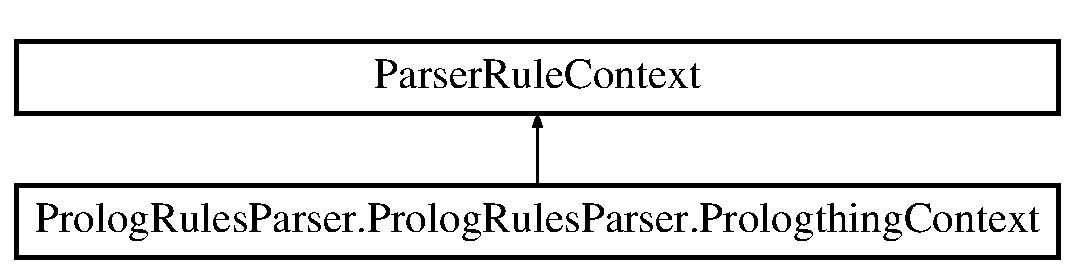
\includegraphics[height=2.000000cm]{class_prolog_rules_parser_1_1_prolog_rules_parser_1_1_prologthing_context}
\end{center}
\end{figure}
\subsection*{Public Member Functions}
\begin{DoxyCompactItemize}
\item 
def \hyperlink{class_prolog_rules_parser_1_1_prolog_rules_parser_1_1_prologthing_context_adcba98eda6d9ed588e5c357bb67f107b}{\+\_\+\+\_\+init\+\_\+\+\_\+}
\item 
def \hyperlink{class_prolog_rules_parser_1_1_prolog_rules_parser_1_1_prologthing_context_acc5e58c7cbf376b3b21a56344448c70d}{constraint} (self)
\item 
def \hyperlink{class_prolog_rules_parser_1_1_prolog_rules_parser_1_1_prologthing_context_a23104f4eb5eb94ef5c5ce75ff04a7ccb}{somerule} (self)
\item 
def \hyperlink{class_prolog_rules_parser_1_1_prolog_rules_parser_1_1_prologthing_context_a1cf4eadb0024fe7ca2eaa14eedb6a913}{fact} (self)
\item 
def \hyperlink{class_prolog_rules_parser_1_1_prolog_rules_parser_1_1_prologthing_context_a958dfdc431e70d22be5a98b07a8a49e3}{get\+Rule\+Index} (self)
\item 
def \hyperlink{class_prolog_rules_parser_1_1_prolog_rules_parser_1_1_prologthing_context_ad793b63974053fe247c6402d508772bf}{enter\+Rule} (self, listener)
\item 
def \hyperlink{class_prolog_rules_parser_1_1_prolog_rules_parser_1_1_prologthing_context_ac51c802ca007aa34f64c23083518150f}{exit\+Rule} (self, listener)
\end{DoxyCompactItemize}
\subsection*{Public Attributes}
\begin{DoxyCompactItemize}
\item 
\hyperlink{class_prolog_rules_parser_1_1_prolog_rules_parser_1_1_prologthing_context_acb9ba47ada7ed08b01eefa6d4142eee7}{parser}
\end{DoxyCompactItemize}


\subsection{Detailed Description}


Definition at line 189 of file Prolog\+Rules\+Parser.\+py.



\subsection{Constructor \& Destructor Documentation}
\hypertarget{class_prolog_rules_parser_1_1_prolog_rules_parser_1_1_prologthing_context_adcba98eda6d9ed588e5c357bb67f107b}{}\index{Prolog\+Rules\+Parser\+::\+Prolog\+Rules\+Parser\+::\+Prologthing\+Context@{Prolog\+Rules\+Parser\+::\+Prolog\+Rules\+Parser\+::\+Prologthing\+Context}!\+\_\+\+\_\+init\+\_\+\+\_\+@{\+\_\+\+\_\+init\+\_\+\+\_\+}}
\index{\+\_\+\+\_\+init\+\_\+\+\_\+@{\+\_\+\+\_\+init\+\_\+\+\_\+}!Prolog\+Rules\+Parser\+::\+Prolog\+Rules\+Parser\+::\+Prologthing\+Context@{Prolog\+Rules\+Parser\+::\+Prolog\+Rules\+Parser\+::\+Prologthing\+Context}}
\subsubsection[{\+\_\+\+\_\+init\+\_\+\+\_\+}]{\setlength{\rightskip}{0pt plus 5cm}def Prolog\+Rules\+Parser.\+Prolog\+Rules\+Parser.\+Prologthing\+Context.\+\_\+\+\_\+init\+\_\+\+\_\+ (
\begin{DoxyParamCaption}
\item[{}]{self, }
\item[{}]{parser, }
\item[{}]{parent = {\ttfamily None}, }
\item[{}]{invoking\+State = {\ttfamily -\/1}}
\end{DoxyParamCaption}
)}\label{class_prolog_rules_parser_1_1_prolog_rules_parser_1_1_prologthing_context_adcba98eda6d9ed588e5c357bb67f107b}


Definition at line 191 of file Prolog\+Rules\+Parser.\+py.



\subsection{Member Function Documentation}
\hypertarget{class_prolog_rules_parser_1_1_prolog_rules_parser_1_1_prologthing_context_acc5e58c7cbf376b3b21a56344448c70d}{}\index{Prolog\+Rules\+Parser\+::\+Prolog\+Rules\+Parser\+::\+Prologthing\+Context@{Prolog\+Rules\+Parser\+::\+Prolog\+Rules\+Parser\+::\+Prologthing\+Context}!constraint@{constraint}}
\index{constraint@{constraint}!Prolog\+Rules\+Parser\+::\+Prolog\+Rules\+Parser\+::\+Prologthing\+Context@{Prolog\+Rules\+Parser\+::\+Prolog\+Rules\+Parser\+::\+Prologthing\+Context}}
\subsubsection[{constraint}]{\setlength{\rightskip}{0pt plus 5cm}def Prolog\+Rules\+Parser.\+Prolog\+Rules\+Parser.\+Prologthing\+Context.\+constraint (
\begin{DoxyParamCaption}
\item[{}]{self}
\end{DoxyParamCaption}
)}\label{class_prolog_rules_parser_1_1_prolog_rules_parser_1_1_prologthing_context_acc5e58c7cbf376b3b21a56344448c70d}


Definition at line 195 of file Prolog\+Rules\+Parser.\+py.

\hypertarget{class_prolog_rules_parser_1_1_prolog_rules_parser_1_1_prologthing_context_ad793b63974053fe247c6402d508772bf}{}\index{Prolog\+Rules\+Parser\+::\+Prolog\+Rules\+Parser\+::\+Prologthing\+Context@{Prolog\+Rules\+Parser\+::\+Prolog\+Rules\+Parser\+::\+Prologthing\+Context}!enter\+Rule@{enter\+Rule}}
\index{enter\+Rule@{enter\+Rule}!Prolog\+Rules\+Parser\+::\+Prolog\+Rules\+Parser\+::\+Prologthing\+Context@{Prolog\+Rules\+Parser\+::\+Prolog\+Rules\+Parser\+::\+Prologthing\+Context}}
\subsubsection[{enter\+Rule}]{\setlength{\rightskip}{0pt plus 5cm}def Prolog\+Rules\+Parser.\+Prolog\+Rules\+Parser.\+Prologthing\+Context.\+enter\+Rule (
\begin{DoxyParamCaption}
\item[{}]{self, }
\item[{}]{listener}
\end{DoxyParamCaption}
)}\label{class_prolog_rules_parser_1_1_prolog_rules_parser_1_1_prologthing_context_ad793b63974053fe247c6402d508772bf}


Definition at line 210 of file Prolog\+Rules\+Parser.\+py.

\hypertarget{class_prolog_rules_parser_1_1_prolog_rules_parser_1_1_prologthing_context_ac51c802ca007aa34f64c23083518150f}{}\index{Prolog\+Rules\+Parser\+::\+Prolog\+Rules\+Parser\+::\+Prologthing\+Context@{Prolog\+Rules\+Parser\+::\+Prolog\+Rules\+Parser\+::\+Prologthing\+Context}!exit\+Rule@{exit\+Rule}}
\index{exit\+Rule@{exit\+Rule}!Prolog\+Rules\+Parser\+::\+Prolog\+Rules\+Parser\+::\+Prologthing\+Context@{Prolog\+Rules\+Parser\+::\+Prolog\+Rules\+Parser\+::\+Prologthing\+Context}}
\subsubsection[{exit\+Rule}]{\setlength{\rightskip}{0pt plus 5cm}def Prolog\+Rules\+Parser.\+Prolog\+Rules\+Parser.\+Prologthing\+Context.\+exit\+Rule (
\begin{DoxyParamCaption}
\item[{}]{self, }
\item[{}]{listener}
\end{DoxyParamCaption}
)}\label{class_prolog_rules_parser_1_1_prolog_rules_parser_1_1_prologthing_context_ac51c802ca007aa34f64c23083518150f}


Definition at line 214 of file Prolog\+Rules\+Parser.\+py.

\hypertarget{class_prolog_rules_parser_1_1_prolog_rules_parser_1_1_prologthing_context_a1cf4eadb0024fe7ca2eaa14eedb6a913}{}\index{Prolog\+Rules\+Parser\+::\+Prolog\+Rules\+Parser\+::\+Prologthing\+Context@{Prolog\+Rules\+Parser\+::\+Prolog\+Rules\+Parser\+::\+Prologthing\+Context}!fact@{fact}}
\index{fact@{fact}!Prolog\+Rules\+Parser\+::\+Prolog\+Rules\+Parser\+::\+Prologthing\+Context@{Prolog\+Rules\+Parser\+::\+Prolog\+Rules\+Parser\+::\+Prologthing\+Context}}
\subsubsection[{fact}]{\setlength{\rightskip}{0pt plus 5cm}def Prolog\+Rules\+Parser.\+Prolog\+Rules\+Parser.\+Prologthing\+Context.\+fact (
\begin{DoxyParamCaption}
\item[{}]{self}
\end{DoxyParamCaption}
)}\label{class_prolog_rules_parser_1_1_prolog_rules_parser_1_1_prologthing_context_a1cf4eadb0024fe7ca2eaa14eedb6a913}


Definition at line 203 of file Prolog\+Rules\+Parser.\+py.

\hypertarget{class_prolog_rules_parser_1_1_prolog_rules_parser_1_1_prologthing_context_a958dfdc431e70d22be5a98b07a8a49e3}{}\index{Prolog\+Rules\+Parser\+::\+Prolog\+Rules\+Parser\+::\+Prologthing\+Context@{Prolog\+Rules\+Parser\+::\+Prolog\+Rules\+Parser\+::\+Prologthing\+Context}!get\+Rule\+Index@{get\+Rule\+Index}}
\index{get\+Rule\+Index@{get\+Rule\+Index}!Prolog\+Rules\+Parser\+::\+Prolog\+Rules\+Parser\+::\+Prologthing\+Context@{Prolog\+Rules\+Parser\+::\+Prolog\+Rules\+Parser\+::\+Prologthing\+Context}}
\subsubsection[{get\+Rule\+Index}]{\setlength{\rightskip}{0pt plus 5cm}def Prolog\+Rules\+Parser.\+Prolog\+Rules\+Parser.\+Prologthing\+Context.\+get\+Rule\+Index (
\begin{DoxyParamCaption}
\item[{}]{self}
\end{DoxyParamCaption}
)}\label{class_prolog_rules_parser_1_1_prolog_rules_parser_1_1_prologthing_context_a958dfdc431e70d22be5a98b07a8a49e3}


Definition at line 207 of file Prolog\+Rules\+Parser.\+py.

\hypertarget{class_prolog_rules_parser_1_1_prolog_rules_parser_1_1_prologthing_context_a23104f4eb5eb94ef5c5ce75ff04a7ccb}{}\index{Prolog\+Rules\+Parser\+::\+Prolog\+Rules\+Parser\+::\+Prologthing\+Context@{Prolog\+Rules\+Parser\+::\+Prolog\+Rules\+Parser\+::\+Prologthing\+Context}!somerule@{somerule}}
\index{somerule@{somerule}!Prolog\+Rules\+Parser\+::\+Prolog\+Rules\+Parser\+::\+Prologthing\+Context@{Prolog\+Rules\+Parser\+::\+Prolog\+Rules\+Parser\+::\+Prologthing\+Context}}
\subsubsection[{somerule}]{\setlength{\rightskip}{0pt plus 5cm}def Prolog\+Rules\+Parser.\+Prolog\+Rules\+Parser.\+Prologthing\+Context.\+somerule (
\begin{DoxyParamCaption}
\item[{}]{self}
\end{DoxyParamCaption}
)}\label{class_prolog_rules_parser_1_1_prolog_rules_parser_1_1_prologthing_context_a23104f4eb5eb94ef5c5ce75ff04a7ccb}


Definition at line 199 of file Prolog\+Rules\+Parser.\+py.



\subsection{Member Data Documentation}
\hypertarget{class_prolog_rules_parser_1_1_prolog_rules_parser_1_1_prologthing_context_acb9ba47ada7ed08b01eefa6d4142eee7}{}\index{Prolog\+Rules\+Parser\+::\+Prolog\+Rules\+Parser\+::\+Prologthing\+Context@{Prolog\+Rules\+Parser\+::\+Prolog\+Rules\+Parser\+::\+Prologthing\+Context}!parser@{parser}}
\index{parser@{parser}!Prolog\+Rules\+Parser\+::\+Prolog\+Rules\+Parser\+::\+Prologthing\+Context@{Prolog\+Rules\+Parser\+::\+Prolog\+Rules\+Parser\+::\+Prologthing\+Context}}
\subsubsection[{parser}]{\setlength{\rightskip}{0pt plus 5cm}Prolog\+Rules\+Parser.\+Prolog\+Rules\+Parser.\+Prologthing\+Context.\+parser}\label{class_prolog_rules_parser_1_1_prolog_rules_parser_1_1_prologthing_context_acb9ba47ada7ed08b01eefa6d4142eee7}


Definition at line 193 of file Prolog\+Rules\+Parser.\+py.



The documentation for this class was generated from the following file\+:\begin{DoxyCompactItemize}
\item 
\hyperlink{_prolog_rules_parser_8py}{Prolog\+Rules\+Parser.\+py}\end{DoxyCompactItemize}

\hypertarget{class_prolog_rules_parser_1_1_prolog_rules_parser_1_1_rulebody_context}{}\section{Prolog\+Rules\+Parser.\+Prolog\+Rules\+Parser.\+Rulebody\+Context Class Reference}
\label{class_prolog_rules_parser_1_1_prolog_rules_parser_1_1_rulebody_context}\index{Prolog\+Rules\+Parser.\+Prolog\+Rules\+Parser.\+Rulebody\+Context@{Prolog\+Rules\+Parser.\+Prolog\+Rules\+Parser.\+Rulebody\+Context}}
Inheritance diagram for Prolog\+Rules\+Parser.\+Prolog\+Rules\+Parser.\+Rulebody\+Context\+:\begin{figure}[H]
\begin{center}
\leavevmode
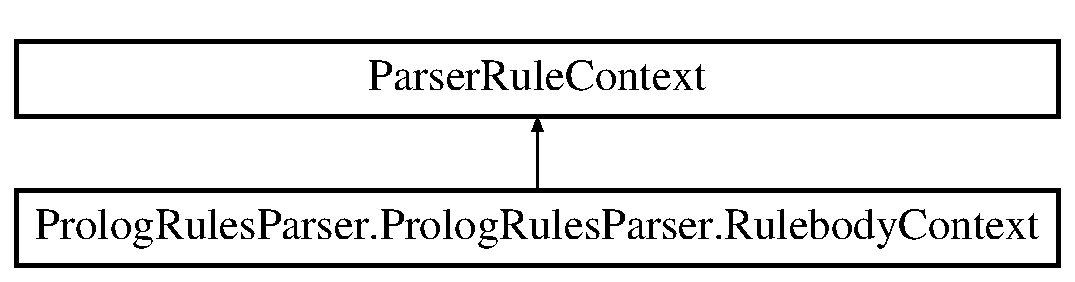
\includegraphics[height=2.000000cm]{class_prolog_rules_parser_1_1_prolog_rules_parser_1_1_rulebody_context}
\end{center}
\end{figure}
\subsection*{Public Member Functions}
\begin{DoxyCompactItemize}
\item 
def \hyperlink{class_prolog_rules_parser_1_1_prolog_rules_parser_1_1_rulebody_context_ae146bb5ff3a101fe95d83ca0a3c2986f}{\+\_\+\+\_\+init\+\_\+\+\_\+}
\item 
def \hyperlink{class_prolog_rules_parser_1_1_prolog_rules_parser_1_1_rulebody_context_af95d4898f23775498a24f4786adeea39}{condition} (self)
\item 
def \hyperlink{class_prolog_rules_parser_1_1_prolog_rules_parser_1_1_rulebody_context_a8a3fe0ec5f2609859b349c123b2ed768}{rulebody} (self)
\item 
def \hyperlink{class_prolog_rules_parser_1_1_prolog_rules_parser_1_1_rulebody_context_a0dfad716e2eae22e6c2f7d1951581c2c}{get\+Rule\+Index} (self)
\item 
def \hyperlink{class_prolog_rules_parser_1_1_prolog_rules_parser_1_1_rulebody_context_ab51b9a6df488dca23f3dcd3107b46f78}{enter\+Rule} (self, listener)
\item 
def \hyperlink{class_prolog_rules_parser_1_1_prolog_rules_parser_1_1_rulebody_context_a1fd2c82516d70578fe3dac7c171c3f82}{exit\+Rule} (self, listener)
\end{DoxyCompactItemize}
\subsection*{Public Attributes}
\begin{DoxyCompactItemize}
\item 
\hyperlink{class_prolog_rules_parser_1_1_prolog_rules_parser_1_1_rulebody_context_a83a2a95c1c09a26d5948fab975b45ddd}{parser}
\end{DoxyCompactItemize}


\subsection{Detailed Description}


Definition at line 675 of file Prolog\+Rules\+Parser.\+py.



\subsection{Constructor \& Destructor Documentation}
\hypertarget{class_prolog_rules_parser_1_1_prolog_rules_parser_1_1_rulebody_context_ae146bb5ff3a101fe95d83ca0a3c2986f}{}\index{Prolog\+Rules\+Parser\+::\+Prolog\+Rules\+Parser\+::\+Rulebody\+Context@{Prolog\+Rules\+Parser\+::\+Prolog\+Rules\+Parser\+::\+Rulebody\+Context}!\+\_\+\+\_\+init\+\_\+\+\_\+@{\+\_\+\+\_\+init\+\_\+\+\_\+}}
\index{\+\_\+\+\_\+init\+\_\+\+\_\+@{\+\_\+\+\_\+init\+\_\+\+\_\+}!Prolog\+Rules\+Parser\+::\+Prolog\+Rules\+Parser\+::\+Rulebody\+Context@{Prolog\+Rules\+Parser\+::\+Prolog\+Rules\+Parser\+::\+Rulebody\+Context}}
\subsubsection[{\+\_\+\+\_\+init\+\_\+\+\_\+}]{\setlength{\rightskip}{0pt plus 5cm}def Prolog\+Rules\+Parser.\+Prolog\+Rules\+Parser.\+Rulebody\+Context.\+\_\+\+\_\+init\+\_\+\+\_\+ (
\begin{DoxyParamCaption}
\item[{}]{self, }
\item[{}]{parser, }
\item[{}]{parent = {\ttfamily None}, }
\item[{}]{invoking\+State = {\ttfamily -\/1}}
\end{DoxyParamCaption}
)}\label{class_prolog_rules_parser_1_1_prolog_rules_parser_1_1_rulebody_context_ae146bb5ff3a101fe95d83ca0a3c2986f}


Definition at line 677 of file Prolog\+Rules\+Parser.\+py.



\subsection{Member Function Documentation}
\hypertarget{class_prolog_rules_parser_1_1_prolog_rules_parser_1_1_rulebody_context_af95d4898f23775498a24f4786adeea39}{}\index{Prolog\+Rules\+Parser\+::\+Prolog\+Rules\+Parser\+::\+Rulebody\+Context@{Prolog\+Rules\+Parser\+::\+Prolog\+Rules\+Parser\+::\+Rulebody\+Context}!condition@{condition}}
\index{condition@{condition}!Prolog\+Rules\+Parser\+::\+Prolog\+Rules\+Parser\+::\+Rulebody\+Context@{Prolog\+Rules\+Parser\+::\+Prolog\+Rules\+Parser\+::\+Rulebody\+Context}}
\subsubsection[{condition}]{\setlength{\rightskip}{0pt plus 5cm}def Prolog\+Rules\+Parser.\+Prolog\+Rules\+Parser.\+Rulebody\+Context.\+condition (
\begin{DoxyParamCaption}
\item[{}]{self}
\end{DoxyParamCaption}
)}\label{class_prolog_rules_parser_1_1_prolog_rules_parser_1_1_rulebody_context_af95d4898f23775498a24f4786adeea39}


Definition at line 681 of file Prolog\+Rules\+Parser.\+py.

\hypertarget{class_prolog_rules_parser_1_1_prolog_rules_parser_1_1_rulebody_context_ab51b9a6df488dca23f3dcd3107b46f78}{}\index{Prolog\+Rules\+Parser\+::\+Prolog\+Rules\+Parser\+::\+Rulebody\+Context@{Prolog\+Rules\+Parser\+::\+Prolog\+Rules\+Parser\+::\+Rulebody\+Context}!enter\+Rule@{enter\+Rule}}
\index{enter\+Rule@{enter\+Rule}!Prolog\+Rules\+Parser\+::\+Prolog\+Rules\+Parser\+::\+Rulebody\+Context@{Prolog\+Rules\+Parser\+::\+Prolog\+Rules\+Parser\+::\+Rulebody\+Context}}
\subsubsection[{enter\+Rule}]{\setlength{\rightskip}{0pt plus 5cm}def Prolog\+Rules\+Parser.\+Prolog\+Rules\+Parser.\+Rulebody\+Context.\+enter\+Rule (
\begin{DoxyParamCaption}
\item[{}]{self, }
\item[{}]{listener}
\end{DoxyParamCaption}
)}\label{class_prolog_rules_parser_1_1_prolog_rules_parser_1_1_rulebody_context_ab51b9a6df488dca23f3dcd3107b46f78}


Definition at line 692 of file Prolog\+Rules\+Parser.\+py.

\hypertarget{class_prolog_rules_parser_1_1_prolog_rules_parser_1_1_rulebody_context_a1fd2c82516d70578fe3dac7c171c3f82}{}\index{Prolog\+Rules\+Parser\+::\+Prolog\+Rules\+Parser\+::\+Rulebody\+Context@{Prolog\+Rules\+Parser\+::\+Prolog\+Rules\+Parser\+::\+Rulebody\+Context}!exit\+Rule@{exit\+Rule}}
\index{exit\+Rule@{exit\+Rule}!Prolog\+Rules\+Parser\+::\+Prolog\+Rules\+Parser\+::\+Rulebody\+Context@{Prolog\+Rules\+Parser\+::\+Prolog\+Rules\+Parser\+::\+Rulebody\+Context}}
\subsubsection[{exit\+Rule}]{\setlength{\rightskip}{0pt plus 5cm}def Prolog\+Rules\+Parser.\+Prolog\+Rules\+Parser.\+Rulebody\+Context.\+exit\+Rule (
\begin{DoxyParamCaption}
\item[{}]{self, }
\item[{}]{listener}
\end{DoxyParamCaption}
)}\label{class_prolog_rules_parser_1_1_prolog_rules_parser_1_1_rulebody_context_a1fd2c82516d70578fe3dac7c171c3f82}


Definition at line 696 of file Prolog\+Rules\+Parser.\+py.

\hypertarget{class_prolog_rules_parser_1_1_prolog_rules_parser_1_1_rulebody_context_a0dfad716e2eae22e6c2f7d1951581c2c}{}\index{Prolog\+Rules\+Parser\+::\+Prolog\+Rules\+Parser\+::\+Rulebody\+Context@{Prolog\+Rules\+Parser\+::\+Prolog\+Rules\+Parser\+::\+Rulebody\+Context}!get\+Rule\+Index@{get\+Rule\+Index}}
\index{get\+Rule\+Index@{get\+Rule\+Index}!Prolog\+Rules\+Parser\+::\+Prolog\+Rules\+Parser\+::\+Rulebody\+Context@{Prolog\+Rules\+Parser\+::\+Prolog\+Rules\+Parser\+::\+Rulebody\+Context}}
\subsubsection[{get\+Rule\+Index}]{\setlength{\rightskip}{0pt plus 5cm}def Prolog\+Rules\+Parser.\+Prolog\+Rules\+Parser.\+Rulebody\+Context.\+get\+Rule\+Index (
\begin{DoxyParamCaption}
\item[{}]{self}
\end{DoxyParamCaption}
)}\label{class_prolog_rules_parser_1_1_prolog_rules_parser_1_1_rulebody_context_a0dfad716e2eae22e6c2f7d1951581c2c}


Definition at line 689 of file Prolog\+Rules\+Parser.\+py.

\hypertarget{class_prolog_rules_parser_1_1_prolog_rules_parser_1_1_rulebody_context_a8a3fe0ec5f2609859b349c123b2ed768}{}\index{Prolog\+Rules\+Parser\+::\+Prolog\+Rules\+Parser\+::\+Rulebody\+Context@{Prolog\+Rules\+Parser\+::\+Prolog\+Rules\+Parser\+::\+Rulebody\+Context}!rulebody@{rulebody}}
\index{rulebody@{rulebody}!Prolog\+Rules\+Parser\+::\+Prolog\+Rules\+Parser\+::\+Rulebody\+Context@{Prolog\+Rules\+Parser\+::\+Prolog\+Rules\+Parser\+::\+Rulebody\+Context}}
\subsubsection[{rulebody}]{\setlength{\rightskip}{0pt plus 5cm}def Prolog\+Rules\+Parser.\+Prolog\+Rules\+Parser.\+Rulebody\+Context.\+rulebody (
\begin{DoxyParamCaption}
\item[{}]{self}
\end{DoxyParamCaption}
)}\label{class_prolog_rules_parser_1_1_prolog_rules_parser_1_1_rulebody_context_a8a3fe0ec5f2609859b349c123b2ed768}


Definition at line 685 of file Prolog\+Rules\+Parser.\+py.



\subsection{Member Data Documentation}
\hypertarget{class_prolog_rules_parser_1_1_prolog_rules_parser_1_1_rulebody_context_a83a2a95c1c09a26d5948fab975b45ddd}{}\index{Prolog\+Rules\+Parser\+::\+Prolog\+Rules\+Parser\+::\+Rulebody\+Context@{Prolog\+Rules\+Parser\+::\+Prolog\+Rules\+Parser\+::\+Rulebody\+Context}!parser@{parser}}
\index{parser@{parser}!Prolog\+Rules\+Parser\+::\+Prolog\+Rules\+Parser\+::\+Rulebody\+Context@{Prolog\+Rules\+Parser\+::\+Prolog\+Rules\+Parser\+::\+Rulebody\+Context}}
\subsubsection[{parser}]{\setlength{\rightskip}{0pt plus 5cm}Prolog\+Rules\+Parser.\+Prolog\+Rules\+Parser.\+Rulebody\+Context.\+parser}\label{class_prolog_rules_parser_1_1_prolog_rules_parser_1_1_rulebody_context_a83a2a95c1c09a26d5948fab975b45ddd}


Definition at line 679 of file Prolog\+Rules\+Parser.\+py.



The documentation for this class was generated from the following file\+:\begin{DoxyCompactItemize}
\item 
\hyperlink{_prolog_rules_parser_8py}{Prolog\+Rules\+Parser.\+py}\end{DoxyCompactItemize}

\hypertarget{classparse__asp__rules_1_1_rule_listener}{}\section{parse\+\_\+asp\+\_\+rules.\+Rule\+Listener Class Reference}
\label{classparse__asp__rules_1_1_rule_listener}\index{parse\+\_\+asp\+\_\+rules.\+Rule\+Listener@{parse\+\_\+asp\+\_\+rules.\+Rule\+Listener}}
Inheritance diagram for parse\+\_\+asp\+\_\+rules.\+Rule\+Listener\+:\begin{figure}[H]
\begin{center}
\leavevmode
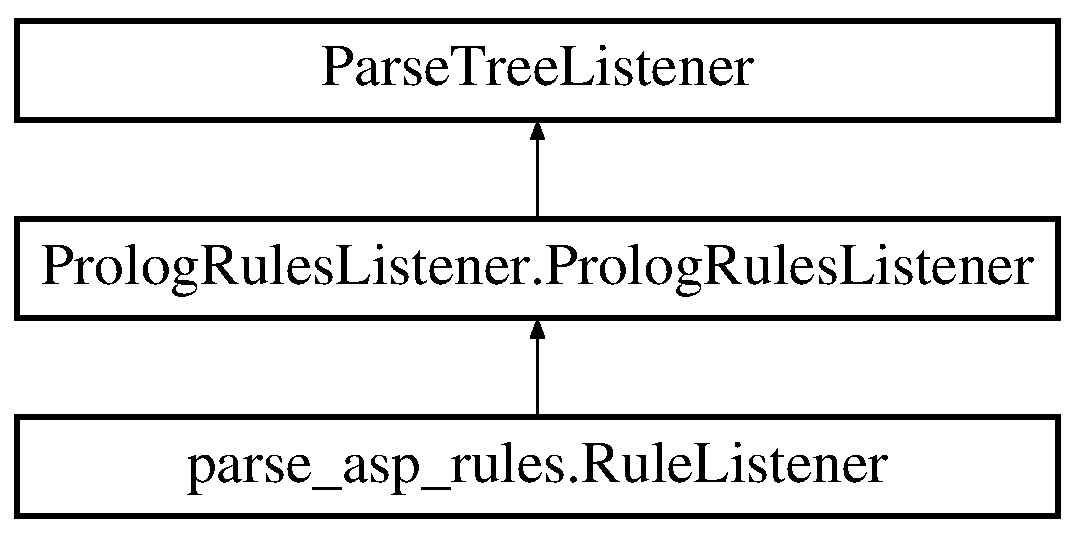
\includegraphics[height=3.000000cm]{classparse__asp__rules_1_1_rule_listener}
\end{center}
\end{figure}
\subsection*{Public Member Functions}
\begin{DoxyCompactItemize}
\item 
def \hyperlink{classparse__asp__rules_1_1_rule_listener_aed6c20fc3c3d74f0c1376613a7ccd20f}{\+\_\+\+\_\+init\+\_\+\+\_\+} (self)
\item 
def \hyperlink{classparse__asp__rules_1_1_rule_listener_a2b9cbc635f40644c6b28baba9e9bc4e9}{enter\+Prologrule} (self, ctx)
\item 
def \hyperlink{classparse__asp__rules_1_1_rule_listener_a08f581c9ffe13176b525255e52c796d0}{exit\+Prologrule} (self, ctx)
\item 
def \hyperlink{classparse__asp__rules_1_1_rule_listener_a820be3f56f380c25b5ff0aeb22e86d26}{enter\+Predicate} (self, ctx)
\item 
def \hyperlink{classparse__asp__rules_1_1_rule_listener_af426f2bb479d05bcd8e92450f2ad0727}{exit\+Predicate} (self, ctx)
\item 
def \hyperlink{classparse__asp__rules_1_1_rule_listener_a79a793d00444872649dc32fb1e818f6d}{enter\+Args} (self, ctx)
\item 
def \hyperlink{classparse__asp__rules_1_1_rule_listener_a6722386aedbdd509047d8c12645c3573}{exit\+Args} (self, ctx)
\item 
def \hyperlink{classparse__asp__rules_1_1_rule_listener_ae19f0844f103ed4a8257353f6f82aec6}{enter\+Comparator} (self, ctx)
\item 
def \hyperlink{classparse__asp__rules_1_1_rule_listener_a2f6e4d416fb7e003559f67a897b7eef9}{exit\+Comparator} (self, ctx)
\item 
def \hyperlink{classparse__asp__rules_1_1_rule_listener_a70653f14a5807e7dfca391537cb58292}{exit\+Negpred} (self, ctx)
\item 
def \hyperlink{classparse__asp__rules_1_1_rule_listener_ae87dd1e8ab64069f895a475960671e56}{exit\+Fact} (self, ctx)
\item 
def \hyperlink{classparse__asp__rules_1_1_rule_listener_a51f78e68592774bb99a9a7438316a57c}{enter\+Constraint} (self, ctx)
\item 
def \hyperlink{classparse__asp__rules_1_1_rule_listener_a8d46ae0d296f1fb63a3497a2133ad622}{exit\+Constraint} (self, ctx)
\item 
def \hyperlink{classparse__asp__rules_1_1_rule_listener_a486d9501f9d43b4ec18087927a4bc0eb}{enter\+Guessrule} (self, ctx)
\item 
def \hyperlink{classparse__asp__rules_1_1_rule_listener_a718018993ecac59520aebec7ae63b73d}{exit\+Guessrule} (self, ctx)
\item 
def \hyperlink{classparse__asp__rules_1_1_rule_listener_a1b2fe6298c4cd441d99211f145b34bd2}{enter\+Predcount} (self, ctx)
\item 
def \hyperlink{classparse__asp__rules_1_1_rule_listener_a73dd7410307759306b77579ef6a4b11c}{isolate\+Predcount\+Data} (self, predcount\+\_\+data)
\item 
def \hyperlink{classparse__asp__rules_1_1_rule_listener_a5ab9bf88929727fb53a67a234394317a}{exit\+Predcount} (self, ctx)
\item 
def \hyperlink{classparse__asp__rules_1_1_rule_listener_a6299867c4fdaca8e5698fadb6e9618f4}{exit\+Atom} (self, ctx)
\item 
def \hyperlink{classparse__asp__rules_1_1_rule_listener_a03c289b66acb0f75f2ed8cccd9f21cc7}{exit\+Identifier} (self, ctx)
\item 
def \hyperlink{classparse__asp__rules_1_1_rule_listener_afc4c08e2209e839cafd4e8afe38693f8}{push\+Container} (self, elem)
\item 
def \hyperlink{classparse__asp__rules_1_1_rule_listener_aad428c830c9b3d41e9e99501156a281f}{pop\+Container} (self)
\item 
def \hyperlink{classparse__asp__rules_1_1_rule_listener_adc1a28101151b8adf07697d8a4a8dd5d}{append\+To\+Last\+Container} (self, elem)
\item 
def \hyperlink{classparse__asp__rules_1_1_rule_listener_a0f1c48df98e762c6f0522acf0ded7a33}{pop\+Last\+Predicate} (self)
\end{DoxyCompactItemize}
\subsection*{Public Attributes}
\begin{DoxyCompactItemize}
\item 
\hyperlink{classparse__asp__rules_1_1_rule_listener_a6923e5b023bb9c94836a12a3bb80f184}{tree}
\item 
\hyperlink{classparse__asp__rules_1_1_rule_listener_a018b6fd2188baceee8498a529d0df9f8}{container\+\_\+stack}
\end{DoxyCompactItemize}


\subsection{Detailed Description}
\begin{DoxyVerb}custom listener will generate list of rules parsed, when passed to a tree walker \end{DoxyVerb}
 

Definition at line 15 of file parse\+\_\+asp\+\_\+rules.\+py.



\subsection{Constructor \& Destructor Documentation}
\hypertarget{classparse__asp__rules_1_1_rule_listener_aed6c20fc3c3d74f0c1376613a7ccd20f}{}\index{parse\+\_\+asp\+\_\+rules\+::\+Rule\+Listener@{parse\+\_\+asp\+\_\+rules\+::\+Rule\+Listener}!\+\_\+\+\_\+init\+\_\+\+\_\+@{\+\_\+\+\_\+init\+\_\+\+\_\+}}
\index{\+\_\+\+\_\+init\+\_\+\+\_\+@{\+\_\+\+\_\+init\+\_\+\+\_\+}!parse\+\_\+asp\+\_\+rules\+::\+Rule\+Listener@{parse\+\_\+asp\+\_\+rules\+::\+Rule\+Listener}}
\subsubsection[{\+\_\+\+\_\+init\+\_\+\+\_\+}]{\setlength{\rightskip}{0pt plus 5cm}def parse\+\_\+asp\+\_\+rules.\+Rule\+Listener.\+\_\+\+\_\+init\+\_\+\+\_\+ (
\begin{DoxyParamCaption}
\item[{}]{self}
\end{DoxyParamCaption}
)}\label{classparse__asp__rules_1_1_rule_listener_aed6c20fc3c3d74f0c1376613a7ccd20f}


Definition at line 17 of file parse\+\_\+asp\+\_\+rules.\+py.



\subsection{Member Function Documentation}
\hypertarget{classparse__asp__rules_1_1_rule_listener_adc1a28101151b8adf07697d8a4a8dd5d}{}\index{parse\+\_\+asp\+\_\+rules\+::\+Rule\+Listener@{parse\+\_\+asp\+\_\+rules\+::\+Rule\+Listener}!append\+To\+Last\+Container@{append\+To\+Last\+Container}}
\index{append\+To\+Last\+Container@{append\+To\+Last\+Container}!parse\+\_\+asp\+\_\+rules\+::\+Rule\+Listener@{parse\+\_\+asp\+\_\+rules\+::\+Rule\+Listener}}
\subsubsection[{append\+To\+Last\+Container}]{\setlength{\rightskip}{0pt plus 5cm}def parse\+\_\+asp\+\_\+rules.\+Rule\+Listener.\+append\+To\+Last\+Container (
\begin{DoxyParamCaption}
\item[{}]{self, }
\item[{}]{elem}
\end{DoxyParamCaption}
)}\label{classparse__asp__rules_1_1_rule_listener_adc1a28101151b8adf07697d8a4a8dd5d}


Definition at line 135 of file parse\+\_\+asp\+\_\+rules.\+py.

\hypertarget{classparse__asp__rules_1_1_rule_listener_a79a793d00444872649dc32fb1e818f6d}{}\index{parse\+\_\+asp\+\_\+rules\+::\+Rule\+Listener@{parse\+\_\+asp\+\_\+rules\+::\+Rule\+Listener}!enter\+Args@{enter\+Args}}
\index{enter\+Args@{enter\+Args}!parse\+\_\+asp\+\_\+rules\+::\+Rule\+Listener@{parse\+\_\+asp\+\_\+rules\+::\+Rule\+Listener}}
\subsubsection[{enter\+Args}]{\setlength{\rightskip}{0pt plus 5cm}def parse\+\_\+asp\+\_\+rules.\+Rule\+Listener.\+enter\+Args (
\begin{DoxyParamCaption}
\item[{}]{self, }
\item[{}]{ctx}
\end{DoxyParamCaption}
)}\label{classparse__asp__rules_1_1_rule_listener_a79a793d00444872649dc32fb1e818f6d}


Definition at line 49 of file parse\+\_\+asp\+\_\+rules.\+py.

\hypertarget{classparse__asp__rules_1_1_rule_listener_ae19f0844f103ed4a8257353f6f82aec6}{}\index{parse\+\_\+asp\+\_\+rules\+::\+Rule\+Listener@{parse\+\_\+asp\+\_\+rules\+::\+Rule\+Listener}!enter\+Comparator@{enter\+Comparator}}
\index{enter\+Comparator@{enter\+Comparator}!parse\+\_\+asp\+\_\+rules\+::\+Rule\+Listener@{parse\+\_\+asp\+\_\+rules\+::\+Rule\+Listener}}
\subsubsection[{enter\+Comparator}]{\setlength{\rightskip}{0pt plus 5cm}def parse\+\_\+asp\+\_\+rules.\+Rule\+Listener.\+enter\+Comparator (
\begin{DoxyParamCaption}
\item[{}]{self, }
\item[{}]{ctx}
\end{DoxyParamCaption}
)}\label{classparse__asp__rules_1_1_rule_listener_ae19f0844f103ed4a8257353f6f82aec6}


Definition at line 55 of file parse\+\_\+asp\+\_\+rules.\+py.

\hypertarget{classparse__asp__rules_1_1_rule_listener_a51f78e68592774bb99a9a7438316a57c}{}\index{parse\+\_\+asp\+\_\+rules\+::\+Rule\+Listener@{parse\+\_\+asp\+\_\+rules\+::\+Rule\+Listener}!enter\+Constraint@{enter\+Constraint}}
\index{enter\+Constraint@{enter\+Constraint}!parse\+\_\+asp\+\_\+rules\+::\+Rule\+Listener@{parse\+\_\+asp\+\_\+rules\+::\+Rule\+Listener}}
\subsubsection[{enter\+Constraint}]{\setlength{\rightskip}{0pt plus 5cm}def parse\+\_\+asp\+\_\+rules.\+Rule\+Listener.\+enter\+Constraint (
\begin{DoxyParamCaption}
\item[{}]{self, }
\item[{}]{ctx}
\end{DoxyParamCaption}
)}\label{classparse__asp__rules_1_1_rule_listener_a51f78e68592774bb99a9a7438316a57c}


Definition at line 73 of file parse\+\_\+asp\+\_\+rules.\+py.

\hypertarget{classparse__asp__rules_1_1_rule_listener_a486d9501f9d43b4ec18087927a4bc0eb}{}\index{parse\+\_\+asp\+\_\+rules\+::\+Rule\+Listener@{parse\+\_\+asp\+\_\+rules\+::\+Rule\+Listener}!enter\+Guessrule@{enter\+Guessrule}}
\index{enter\+Guessrule@{enter\+Guessrule}!parse\+\_\+asp\+\_\+rules\+::\+Rule\+Listener@{parse\+\_\+asp\+\_\+rules\+::\+Rule\+Listener}}
\subsubsection[{enter\+Guessrule}]{\setlength{\rightskip}{0pt plus 5cm}def parse\+\_\+asp\+\_\+rules.\+Rule\+Listener.\+enter\+Guessrule (
\begin{DoxyParamCaption}
\item[{}]{self, }
\item[{}]{ctx}
\end{DoxyParamCaption}
)}\label{classparse__asp__rules_1_1_rule_listener_a486d9501f9d43b4ec18087927a4bc0eb}


Definition at line 78 of file parse\+\_\+asp\+\_\+rules.\+py.

\hypertarget{classparse__asp__rules_1_1_rule_listener_a1b2fe6298c4cd441d99211f145b34bd2}{}\index{parse\+\_\+asp\+\_\+rules\+::\+Rule\+Listener@{parse\+\_\+asp\+\_\+rules\+::\+Rule\+Listener}!enter\+Predcount@{enter\+Predcount}}
\index{enter\+Predcount@{enter\+Predcount}!parse\+\_\+asp\+\_\+rules\+::\+Rule\+Listener@{parse\+\_\+asp\+\_\+rules\+::\+Rule\+Listener}}
\subsubsection[{enter\+Predcount}]{\setlength{\rightskip}{0pt plus 5cm}def parse\+\_\+asp\+\_\+rules.\+Rule\+Listener.\+enter\+Predcount (
\begin{DoxyParamCaption}
\item[{}]{self, }
\item[{}]{ctx}
\end{DoxyParamCaption}
)}\label{classparse__asp__rules_1_1_rule_listener_a1b2fe6298c4cd441d99211f145b34bd2}


Definition at line 83 of file parse\+\_\+asp\+\_\+rules.\+py.

\hypertarget{classparse__asp__rules_1_1_rule_listener_a820be3f56f380c25b5ff0aeb22e86d26}{}\index{parse\+\_\+asp\+\_\+rules\+::\+Rule\+Listener@{parse\+\_\+asp\+\_\+rules\+::\+Rule\+Listener}!enter\+Predicate@{enter\+Predicate}}
\index{enter\+Predicate@{enter\+Predicate}!parse\+\_\+asp\+\_\+rules\+::\+Rule\+Listener@{parse\+\_\+asp\+\_\+rules\+::\+Rule\+Listener}}
\subsubsection[{enter\+Predicate}]{\setlength{\rightskip}{0pt plus 5cm}def parse\+\_\+asp\+\_\+rules.\+Rule\+Listener.\+enter\+Predicate (
\begin{DoxyParamCaption}
\item[{}]{self, }
\item[{}]{ctx}
\end{DoxyParamCaption}
)}\label{classparse__asp__rules_1_1_rule_listener_a820be3f56f380c25b5ff0aeb22e86d26}


Definition at line 36 of file parse\+\_\+asp\+\_\+rules.\+py.

\hypertarget{classparse__asp__rules_1_1_rule_listener_a2b9cbc635f40644c6b28baba9e9bc4e9}{}\index{parse\+\_\+asp\+\_\+rules\+::\+Rule\+Listener@{parse\+\_\+asp\+\_\+rules\+::\+Rule\+Listener}!enter\+Prologrule@{enter\+Prologrule}}
\index{enter\+Prologrule@{enter\+Prologrule}!parse\+\_\+asp\+\_\+rules\+::\+Rule\+Listener@{parse\+\_\+asp\+\_\+rules\+::\+Rule\+Listener}}
\subsubsection[{enter\+Prologrule}]{\setlength{\rightskip}{0pt plus 5cm}def parse\+\_\+asp\+\_\+rules.\+Rule\+Listener.\+enter\+Prologrule (
\begin{DoxyParamCaption}
\item[{}]{self, }
\item[{}]{ctx}
\end{DoxyParamCaption}
)}\label{classparse__asp__rules_1_1_rule_listener_a2b9cbc635f40644c6b28baba9e9bc4e9}


Definition at line 29 of file parse\+\_\+asp\+\_\+rules.\+py.

\hypertarget{classparse__asp__rules_1_1_rule_listener_a6722386aedbdd509047d8c12645c3573}{}\index{parse\+\_\+asp\+\_\+rules\+::\+Rule\+Listener@{parse\+\_\+asp\+\_\+rules\+::\+Rule\+Listener}!exit\+Args@{exit\+Args}}
\index{exit\+Args@{exit\+Args}!parse\+\_\+asp\+\_\+rules\+::\+Rule\+Listener@{parse\+\_\+asp\+\_\+rules\+::\+Rule\+Listener}}
\subsubsection[{exit\+Args}]{\setlength{\rightskip}{0pt plus 5cm}def parse\+\_\+asp\+\_\+rules.\+Rule\+Listener.\+exit\+Args (
\begin{DoxyParamCaption}
\item[{}]{self, }
\item[{}]{ctx}
\end{DoxyParamCaption}
)}\label{classparse__asp__rules_1_1_rule_listener_a6722386aedbdd509047d8c12645c3573}


Definition at line 51 of file parse\+\_\+asp\+\_\+rules.\+py.

\hypertarget{classparse__asp__rules_1_1_rule_listener_a6299867c4fdaca8e5698fadb6e9618f4}{}\index{parse\+\_\+asp\+\_\+rules\+::\+Rule\+Listener@{parse\+\_\+asp\+\_\+rules\+::\+Rule\+Listener}!exit\+Atom@{exit\+Atom}}
\index{exit\+Atom@{exit\+Atom}!parse\+\_\+asp\+\_\+rules\+::\+Rule\+Listener@{parse\+\_\+asp\+\_\+rules\+::\+Rule\+Listener}}
\subsubsection[{exit\+Atom}]{\setlength{\rightskip}{0pt plus 5cm}def parse\+\_\+asp\+\_\+rules.\+Rule\+Listener.\+exit\+Atom (
\begin{DoxyParamCaption}
\item[{}]{self, }
\item[{}]{ctx}
\end{DoxyParamCaption}
)}\label{classparse__asp__rules_1_1_rule_listener_a6299867c4fdaca8e5698fadb6e9618f4}


Definition at line 119 of file parse\+\_\+asp\+\_\+rules.\+py.

\hypertarget{classparse__asp__rules_1_1_rule_listener_a2f6e4d416fb7e003559f67a897b7eef9}{}\index{parse\+\_\+asp\+\_\+rules\+::\+Rule\+Listener@{parse\+\_\+asp\+\_\+rules\+::\+Rule\+Listener}!exit\+Comparator@{exit\+Comparator}}
\index{exit\+Comparator@{exit\+Comparator}!parse\+\_\+asp\+\_\+rules\+::\+Rule\+Listener@{parse\+\_\+asp\+\_\+rules\+::\+Rule\+Listener}}
\subsubsection[{exit\+Comparator}]{\setlength{\rightskip}{0pt plus 5cm}def parse\+\_\+asp\+\_\+rules.\+Rule\+Listener.\+exit\+Comparator (
\begin{DoxyParamCaption}
\item[{}]{self, }
\item[{}]{ctx}
\end{DoxyParamCaption}
)}\label{classparse__asp__rules_1_1_rule_listener_a2f6e4d416fb7e003559f67a897b7eef9}


Definition at line 57 of file parse\+\_\+asp\+\_\+rules.\+py.

\hypertarget{classparse__asp__rules_1_1_rule_listener_a8d46ae0d296f1fb63a3497a2133ad622}{}\index{parse\+\_\+asp\+\_\+rules\+::\+Rule\+Listener@{parse\+\_\+asp\+\_\+rules\+::\+Rule\+Listener}!exit\+Constraint@{exit\+Constraint}}
\index{exit\+Constraint@{exit\+Constraint}!parse\+\_\+asp\+\_\+rules\+::\+Rule\+Listener@{parse\+\_\+asp\+\_\+rules\+::\+Rule\+Listener}}
\subsubsection[{exit\+Constraint}]{\setlength{\rightskip}{0pt plus 5cm}def parse\+\_\+asp\+\_\+rules.\+Rule\+Listener.\+exit\+Constraint (
\begin{DoxyParamCaption}
\item[{}]{self, }
\item[{}]{ctx}
\end{DoxyParamCaption}
)}\label{classparse__asp__rules_1_1_rule_listener_a8d46ae0d296f1fb63a3497a2133ad622}


Definition at line 75 of file parse\+\_\+asp\+\_\+rules.\+py.

\hypertarget{classparse__asp__rules_1_1_rule_listener_ae87dd1e8ab64069f895a475960671e56}{}\index{parse\+\_\+asp\+\_\+rules\+::\+Rule\+Listener@{parse\+\_\+asp\+\_\+rules\+::\+Rule\+Listener}!exit\+Fact@{exit\+Fact}}
\index{exit\+Fact@{exit\+Fact}!parse\+\_\+asp\+\_\+rules\+::\+Rule\+Listener@{parse\+\_\+asp\+\_\+rules\+::\+Rule\+Listener}}
\subsubsection[{exit\+Fact}]{\setlength{\rightskip}{0pt plus 5cm}def parse\+\_\+asp\+\_\+rules.\+Rule\+Listener.\+exit\+Fact (
\begin{DoxyParamCaption}
\item[{}]{self, }
\item[{}]{ctx}
\end{DoxyParamCaption}
)}\label{classparse__asp__rules_1_1_rule_listener_ae87dd1e8ab64069f895a475960671e56}


Definition at line 71 of file parse\+\_\+asp\+\_\+rules.\+py.

\hypertarget{classparse__asp__rules_1_1_rule_listener_a718018993ecac59520aebec7ae63b73d}{}\index{parse\+\_\+asp\+\_\+rules\+::\+Rule\+Listener@{parse\+\_\+asp\+\_\+rules\+::\+Rule\+Listener}!exit\+Guessrule@{exit\+Guessrule}}
\index{exit\+Guessrule@{exit\+Guessrule}!parse\+\_\+asp\+\_\+rules\+::\+Rule\+Listener@{parse\+\_\+asp\+\_\+rules\+::\+Rule\+Listener}}
\subsubsection[{exit\+Guessrule}]{\setlength{\rightskip}{0pt plus 5cm}def parse\+\_\+asp\+\_\+rules.\+Rule\+Listener.\+exit\+Guessrule (
\begin{DoxyParamCaption}
\item[{}]{self, }
\item[{}]{ctx}
\end{DoxyParamCaption}
)}\label{classparse__asp__rules_1_1_rule_listener_a718018993ecac59520aebec7ae63b73d}


Definition at line 80 of file parse\+\_\+asp\+\_\+rules.\+py.

\hypertarget{classparse__asp__rules_1_1_rule_listener_a03c289b66acb0f75f2ed8cccd9f21cc7}{}\index{parse\+\_\+asp\+\_\+rules\+::\+Rule\+Listener@{parse\+\_\+asp\+\_\+rules\+::\+Rule\+Listener}!exit\+Identifier@{exit\+Identifier}}
\index{exit\+Identifier@{exit\+Identifier}!parse\+\_\+asp\+\_\+rules\+::\+Rule\+Listener@{parse\+\_\+asp\+\_\+rules\+::\+Rule\+Listener}}
\subsubsection[{exit\+Identifier}]{\setlength{\rightskip}{0pt plus 5cm}def parse\+\_\+asp\+\_\+rules.\+Rule\+Listener.\+exit\+Identifier (
\begin{DoxyParamCaption}
\item[{}]{self, }
\item[{}]{ctx}
\end{DoxyParamCaption}
)}\label{classparse__asp__rules_1_1_rule_listener_a03c289b66acb0f75f2ed8cccd9f21cc7}


Definition at line 123 of file parse\+\_\+asp\+\_\+rules.\+py.

\hypertarget{classparse__asp__rules_1_1_rule_listener_a70653f14a5807e7dfca391537cb58292}{}\index{parse\+\_\+asp\+\_\+rules\+::\+Rule\+Listener@{parse\+\_\+asp\+\_\+rules\+::\+Rule\+Listener}!exit\+Negpred@{exit\+Negpred}}
\index{exit\+Negpred@{exit\+Negpred}!parse\+\_\+asp\+\_\+rules\+::\+Rule\+Listener@{parse\+\_\+asp\+\_\+rules\+::\+Rule\+Listener}}
\subsubsection[{exit\+Negpred}]{\setlength{\rightskip}{0pt plus 5cm}def parse\+\_\+asp\+\_\+rules.\+Rule\+Listener.\+exit\+Negpred (
\begin{DoxyParamCaption}
\item[{}]{self, }
\item[{}]{ctx}
\end{DoxyParamCaption}
)}\label{classparse__asp__rules_1_1_rule_listener_a70653f14a5807e7dfca391537cb58292}


Definition at line 63 of file parse\+\_\+asp\+\_\+rules.\+py.

\hypertarget{classparse__asp__rules_1_1_rule_listener_a5ab9bf88929727fb53a67a234394317a}{}\index{parse\+\_\+asp\+\_\+rules\+::\+Rule\+Listener@{parse\+\_\+asp\+\_\+rules\+::\+Rule\+Listener}!exit\+Predcount@{exit\+Predcount}}
\index{exit\+Predcount@{exit\+Predcount}!parse\+\_\+asp\+\_\+rules\+::\+Rule\+Listener@{parse\+\_\+asp\+\_\+rules\+::\+Rule\+Listener}}
\subsubsection[{exit\+Predcount}]{\setlength{\rightskip}{0pt plus 5cm}def parse\+\_\+asp\+\_\+rules.\+Rule\+Listener.\+exit\+Predcount (
\begin{DoxyParamCaption}
\item[{}]{self, }
\item[{}]{ctx}
\end{DoxyParamCaption}
)}\label{classparse__asp__rules_1_1_rule_listener_a5ab9bf88929727fb53a67a234394317a}


Definition at line 112 of file parse\+\_\+asp\+\_\+rules.\+py.

\hypertarget{classparse__asp__rules_1_1_rule_listener_af426f2bb479d05bcd8e92450f2ad0727}{}\index{parse\+\_\+asp\+\_\+rules\+::\+Rule\+Listener@{parse\+\_\+asp\+\_\+rules\+::\+Rule\+Listener}!exit\+Predicate@{exit\+Predicate}}
\index{exit\+Predicate@{exit\+Predicate}!parse\+\_\+asp\+\_\+rules\+::\+Rule\+Listener@{parse\+\_\+asp\+\_\+rules\+::\+Rule\+Listener}}
\subsubsection[{exit\+Predicate}]{\setlength{\rightskip}{0pt plus 5cm}def parse\+\_\+asp\+\_\+rules.\+Rule\+Listener.\+exit\+Predicate (
\begin{DoxyParamCaption}
\item[{}]{self, }
\item[{}]{ctx}
\end{DoxyParamCaption}
)}\label{classparse__asp__rules_1_1_rule_listener_af426f2bb479d05bcd8e92450f2ad0727}


Definition at line 38 of file parse\+\_\+asp\+\_\+rules.\+py.

\hypertarget{classparse__asp__rules_1_1_rule_listener_a08f581c9ffe13176b525255e52c796d0}{}\index{parse\+\_\+asp\+\_\+rules\+::\+Rule\+Listener@{parse\+\_\+asp\+\_\+rules\+::\+Rule\+Listener}!exit\+Prologrule@{exit\+Prologrule}}
\index{exit\+Prologrule@{exit\+Prologrule}!parse\+\_\+asp\+\_\+rules\+::\+Rule\+Listener@{parse\+\_\+asp\+\_\+rules\+::\+Rule\+Listener}}
\subsubsection[{exit\+Prologrule}]{\setlength{\rightskip}{0pt plus 5cm}def parse\+\_\+asp\+\_\+rules.\+Rule\+Listener.\+exit\+Prologrule (
\begin{DoxyParamCaption}
\item[{}]{self, }
\item[{}]{ctx}
\end{DoxyParamCaption}
)}\label{classparse__asp__rules_1_1_rule_listener_a08f581c9ffe13176b525255e52c796d0}


Definition at line 31 of file parse\+\_\+asp\+\_\+rules.\+py.

\hypertarget{classparse__asp__rules_1_1_rule_listener_a73dd7410307759306b77579ef6a4b11c}{}\index{parse\+\_\+asp\+\_\+rules\+::\+Rule\+Listener@{parse\+\_\+asp\+\_\+rules\+::\+Rule\+Listener}!isolate\+Predcount\+Data@{isolate\+Predcount\+Data}}
\index{isolate\+Predcount\+Data@{isolate\+Predcount\+Data}!parse\+\_\+asp\+\_\+rules\+::\+Rule\+Listener@{parse\+\_\+asp\+\_\+rules\+::\+Rule\+Listener}}
\subsubsection[{isolate\+Predcount\+Data}]{\setlength{\rightskip}{0pt plus 5cm}def parse\+\_\+asp\+\_\+rules.\+Rule\+Listener.\+isolate\+Predcount\+Data (
\begin{DoxyParamCaption}
\item[{}]{self, }
\item[{}]{predcount\+\_\+data}
\end{DoxyParamCaption}
)}\label{classparse__asp__rules_1_1_rule_listener_a73dd7410307759306b77579ef6a4b11c}
\begin{DoxyVerb}Isolate predcount data from a parse tree walk.
    predcount_data may look like: [left_count, head, body, right_count].
    Only head is guaranteed to exist, anything else will exist in that relative order if at all.
\end{DoxyVerb}
 

Definition at line 85 of file parse\+\_\+asp\+\_\+rules.\+py.

\hypertarget{classparse__asp__rules_1_1_rule_listener_aad428c830c9b3d41e9e99501156a281f}{}\index{parse\+\_\+asp\+\_\+rules\+::\+Rule\+Listener@{parse\+\_\+asp\+\_\+rules\+::\+Rule\+Listener}!pop\+Container@{pop\+Container}}
\index{pop\+Container@{pop\+Container}!parse\+\_\+asp\+\_\+rules\+::\+Rule\+Listener@{parse\+\_\+asp\+\_\+rules\+::\+Rule\+Listener}}
\subsubsection[{pop\+Container}]{\setlength{\rightskip}{0pt plus 5cm}def parse\+\_\+asp\+\_\+rules.\+Rule\+Listener.\+pop\+Container (
\begin{DoxyParamCaption}
\item[{}]{self}
\end{DoxyParamCaption}
)}\label{classparse__asp__rules_1_1_rule_listener_aad428c830c9b3d41e9e99501156a281f}


Definition at line 131 of file parse\+\_\+asp\+\_\+rules.\+py.

\hypertarget{classparse__asp__rules_1_1_rule_listener_a0f1c48df98e762c6f0522acf0ded7a33}{}\index{parse\+\_\+asp\+\_\+rules\+::\+Rule\+Listener@{parse\+\_\+asp\+\_\+rules\+::\+Rule\+Listener}!pop\+Last\+Predicate@{pop\+Last\+Predicate}}
\index{pop\+Last\+Predicate@{pop\+Last\+Predicate}!parse\+\_\+asp\+\_\+rules\+::\+Rule\+Listener@{parse\+\_\+asp\+\_\+rules\+::\+Rule\+Listener}}
\subsubsection[{pop\+Last\+Predicate}]{\setlength{\rightskip}{0pt plus 5cm}def parse\+\_\+asp\+\_\+rules.\+Rule\+Listener.\+pop\+Last\+Predicate (
\begin{DoxyParamCaption}
\item[{}]{self}
\end{DoxyParamCaption}
)}\label{classparse__asp__rules_1_1_rule_listener_a0f1c48df98e762c6f0522acf0ded7a33}


Definition at line 138 of file parse\+\_\+asp\+\_\+rules.\+py.

\hypertarget{classparse__asp__rules_1_1_rule_listener_afc4c08e2209e839cafd4e8afe38693f8}{}\index{parse\+\_\+asp\+\_\+rules\+::\+Rule\+Listener@{parse\+\_\+asp\+\_\+rules\+::\+Rule\+Listener}!push\+Container@{push\+Container}}
\index{push\+Container@{push\+Container}!parse\+\_\+asp\+\_\+rules\+::\+Rule\+Listener@{parse\+\_\+asp\+\_\+rules\+::\+Rule\+Listener}}
\subsubsection[{push\+Container}]{\setlength{\rightskip}{0pt plus 5cm}def parse\+\_\+asp\+\_\+rules.\+Rule\+Listener.\+push\+Container (
\begin{DoxyParamCaption}
\item[{}]{self, }
\item[{}]{elem}
\end{DoxyParamCaption}
)}\label{classparse__asp__rules_1_1_rule_listener_afc4c08e2209e839cafd4e8afe38693f8}


Definition at line 128 of file parse\+\_\+asp\+\_\+rules.\+py.



\subsection{Member Data Documentation}
\hypertarget{classparse__asp__rules_1_1_rule_listener_a018b6fd2188baceee8498a529d0df9f8}{}\index{parse\+\_\+asp\+\_\+rules\+::\+Rule\+Listener@{parse\+\_\+asp\+\_\+rules\+::\+Rule\+Listener}!container\+\_\+stack@{container\+\_\+stack}}
\index{container\+\_\+stack@{container\+\_\+stack}!parse\+\_\+asp\+\_\+rules\+::\+Rule\+Listener@{parse\+\_\+asp\+\_\+rules\+::\+Rule\+Listener}}
\subsubsection[{container\+\_\+stack}]{\setlength{\rightskip}{0pt plus 5cm}parse\+\_\+asp\+\_\+rules.\+Rule\+Listener.\+container\+\_\+stack}\label{classparse__asp__rules_1_1_rule_listener_a018b6fd2188baceee8498a529d0df9f8}


Definition at line 26 of file parse\+\_\+asp\+\_\+rules.\+py.

\hypertarget{classparse__asp__rules_1_1_rule_listener_a6923e5b023bb9c94836a12a3bb80f184}{}\index{parse\+\_\+asp\+\_\+rules\+::\+Rule\+Listener@{parse\+\_\+asp\+\_\+rules\+::\+Rule\+Listener}!tree@{tree}}
\index{tree@{tree}!parse\+\_\+asp\+\_\+rules\+::\+Rule\+Listener@{parse\+\_\+asp\+\_\+rules\+::\+Rule\+Listener}}
\subsubsection[{tree}]{\setlength{\rightskip}{0pt plus 5cm}parse\+\_\+asp\+\_\+rules.\+Rule\+Listener.\+tree}\label{classparse__asp__rules_1_1_rule_listener_a6923e5b023bb9c94836a12a3bb80f184}


Definition at line 19 of file parse\+\_\+asp\+\_\+rules.\+py.



The documentation for this class was generated from the following file\+:\begin{DoxyCompactItemize}
\item 
\hyperlink{parse__asp__rules_8py}{parse\+\_\+asp\+\_\+rules.\+py}\end{DoxyCompactItemize}

\hypertarget{class_prolog_rules_parser_1_1_prolog_rules_parser_1_1_somerule_context}{}\section{Prolog\+Rules\+Parser.\+Prolog\+Rules\+Parser.\+Somerule\+Context Class Reference}
\label{class_prolog_rules_parser_1_1_prolog_rules_parser_1_1_somerule_context}\index{Prolog\+Rules\+Parser.\+Prolog\+Rules\+Parser.\+Somerule\+Context@{Prolog\+Rules\+Parser.\+Prolog\+Rules\+Parser.\+Somerule\+Context}}
Inheritance diagram for Prolog\+Rules\+Parser.\+Prolog\+Rules\+Parser.\+Somerule\+Context\+:\begin{figure}[H]
\begin{center}
\leavevmode
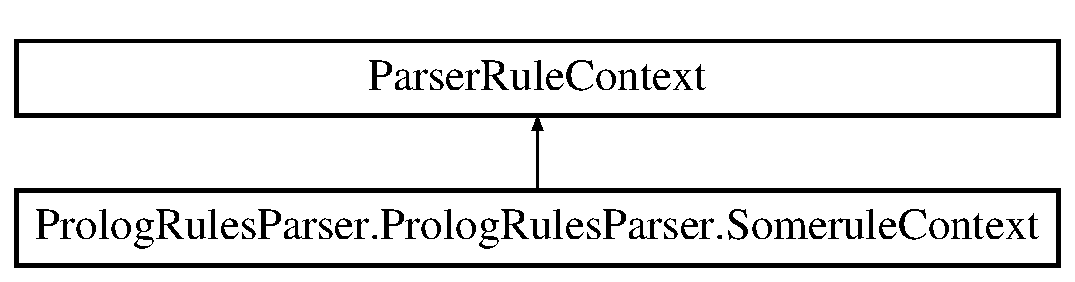
\includegraphics[height=2.000000cm]{class_prolog_rules_parser_1_1_prolog_rules_parser_1_1_somerule_context}
\end{center}
\end{figure}
\subsection*{Public Member Functions}
\begin{DoxyCompactItemize}
\item 
def \hyperlink{class_prolog_rules_parser_1_1_prolog_rules_parser_1_1_somerule_context_a25a5a92579e005d3071c05bd345b8cff}{\+\_\+\+\_\+init\+\_\+\+\_\+}
\item 
def \hyperlink{class_prolog_rules_parser_1_1_prolog_rules_parser_1_1_somerule_context_acd836c262671089eb35e6eb1bcec9f8a}{guessrule} (self)
\item 
def \hyperlink{class_prolog_rules_parser_1_1_prolog_rules_parser_1_1_somerule_context_a1430dbc83eb2764af7b3413a945b91ec}{prologrule} (self)
\item 
def \hyperlink{class_prolog_rules_parser_1_1_prolog_rules_parser_1_1_somerule_context_afe07936790df4597a235fcd83cdd7c2e}{get\+Rule\+Index} (self)
\item 
def \hyperlink{class_prolog_rules_parser_1_1_prolog_rules_parser_1_1_somerule_context_ab711e8ecb7bfc9c5083e5b23095db2f0}{enter\+Rule} (self, listener)
\item 
def \hyperlink{class_prolog_rules_parser_1_1_prolog_rules_parser_1_1_somerule_context_a69339162cbcdd6d4fa5fd21250f5b877}{exit\+Rule} (self, listener)
\end{DoxyCompactItemize}
\subsection*{Public Attributes}
\begin{DoxyCompactItemize}
\item 
\hyperlink{class_prolog_rules_parser_1_1_prolog_rules_parser_1_1_somerule_context_a88cf336f82f18608f2981ba9ee11d4d8}{parser}
\end{DoxyCompactItemize}


\subsection{Detailed Description}


Definition at line 341 of file Prolog\+Rules\+Parser.\+py.



\subsection{Constructor \& Destructor Documentation}
\hypertarget{class_prolog_rules_parser_1_1_prolog_rules_parser_1_1_somerule_context_a25a5a92579e005d3071c05bd345b8cff}{}\index{Prolog\+Rules\+Parser\+::\+Prolog\+Rules\+Parser\+::\+Somerule\+Context@{Prolog\+Rules\+Parser\+::\+Prolog\+Rules\+Parser\+::\+Somerule\+Context}!\+\_\+\+\_\+init\+\_\+\+\_\+@{\+\_\+\+\_\+init\+\_\+\+\_\+}}
\index{\+\_\+\+\_\+init\+\_\+\+\_\+@{\+\_\+\+\_\+init\+\_\+\+\_\+}!Prolog\+Rules\+Parser\+::\+Prolog\+Rules\+Parser\+::\+Somerule\+Context@{Prolog\+Rules\+Parser\+::\+Prolog\+Rules\+Parser\+::\+Somerule\+Context}}
\subsubsection[{\+\_\+\+\_\+init\+\_\+\+\_\+}]{\setlength{\rightskip}{0pt plus 5cm}def Prolog\+Rules\+Parser.\+Prolog\+Rules\+Parser.\+Somerule\+Context.\+\_\+\+\_\+init\+\_\+\+\_\+ (
\begin{DoxyParamCaption}
\item[{}]{self, }
\item[{}]{parser, }
\item[{}]{parent = {\ttfamily None}, }
\item[{}]{invoking\+State = {\ttfamily -\/1}}
\end{DoxyParamCaption}
)}\label{class_prolog_rules_parser_1_1_prolog_rules_parser_1_1_somerule_context_a25a5a92579e005d3071c05bd345b8cff}


Definition at line 343 of file Prolog\+Rules\+Parser.\+py.



\subsection{Member Function Documentation}
\hypertarget{class_prolog_rules_parser_1_1_prolog_rules_parser_1_1_somerule_context_ab711e8ecb7bfc9c5083e5b23095db2f0}{}\index{Prolog\+Rules\+Parser\+::\+Prolog\+Rules\+Parser\+::\+Somerule\+Context@{Prolog\+Rules\+Parser\+::\+Prolog\+Rules\+Parser\+::\+Somerule\+Context}!enter\+Rule@{enter\+Rule}}
\index{enter\+Rule@{enter\+Rule}!Prolog\+Rules\+Parser\+::\+Prolog\+Rules\+Parser\+::\+Somerule\+Context@{Prolog\+Rules\+Parser\+::\+Prolog\+Rules\+Parser\+::\+Somerule\+Context}}
\subsubsection[{enter\+Rule}]{\setlength{\rightskip}{0pt plus 5cm}def Prolog\+Rules\+Parser.\+Prolog\+Rules\+Parser.\+Somerule\+Context.\+enter\+Rule (
\begin{DoxyParamCaption}
\item[{}]{self, }
\item[{}]{listener}
\end{DoxyParamCaption}
)}\label{class_prolog_rules_parser_1_1_prolog_rules_parser_1_1_somerule_context_ab711e8ecb7bfc9c5083e5b23095db2f0}


Definition at line 358 of file Prolog\+Rules\+Parser.\+py.

\hypertarget{class_prolog_rules_parser_1_1_prolog_rules_parser_1_1_somerule_context_a69339162cbcdd6d4fa5fd21250f5b877}{}\index{Prolog\+Rules\+Parser\+::\+Prolog\+Rules\+Parser\+::\+Somerule\+Context@{Prolog\+Rules\+Parser\+::\+Prolog\+Rules\+Parser\+::\+Somerule\+Context}!exit\+Rule@{exit\+Rule}}
\index{exit\+Rule@{exit\+Rule}!Prolog\+Rules\+Parser\+::\+Prolog\+Rules\+Parser\+::\+Somerule\+Context@{Prolog\+Rules\+Parser\+::\+Prolog\+Rules\+Parser\+::\+Somerule\+Context}}
\subsubsection[{exit\+Rule}]{\setlength{\rightskip}{0pt plus 5cm}def Prolog\+Rules\+Parser.\+Prolog\+Rules\+Parser.\+Somerule\+Context.\+exit\+Rule (
\begin{DoxyParamCaption}
\item[{}]{self, }
\item[{}]{listener}
\end{DoxyParamCaption}
)}\label{class_prolog_rules_parser_1_1_prolog_rules_parser_1_1_somerule_context_a69339162cbcdd6d4fa5fd21250f5b877}


Definition at line 362 of file Prolog\+Rules\+Parser.\+py.

\hypertarget{class_prolog_rules_parser_1_1_prolog_rules_parser_1_1_somerule_context_afe07936790df4597a235fcd83cdd7c2e}{}\index{Prolog\+Rules\+Parser\+::\+Prolog\+Rules\+Parser\+::\+Somerule\+Context@{Prolog\+Rules\+Parser\+::\+Prolog\+Rules\+Parser\+::\+Somerule\+Context}!get\+Rule\+Index@{get\+Rule\+Index}}
\index{get\+Rule\+Index@{get\+Rule\+Index}!Prolog\+Rules\+Parser\+::\+Prolog\+Rules\+Parser\+::\+Somerule\+Context@{Prolog\+Rules\+Parser\+::\+Prolog\+Rules\+Parser\+::\+Somerule\+Context}}
\subsubsection[{get\+Rule\+Index}]{\setlength{\rightskip}{0pt plus 5cm}def Prolog\+Rules\+Parser.\+Prolog\+Rules\+Parser.\+Somerule\+Context.\+get\+Rule\+Index (
\begin{DoxyParamCaption}
\item[{}]{self}
\end{DoxyParamCaption}
)}\label{class_prolog_rules_parser_1_1_prolog_rules_parser_1_1_somerule_context_afe07936790df4597a235fcd83cdd7c2e}


Definition at line 355 of file Prolog\+Rules\+Parser.\+py.

\hypertarget{class_prolog_rules_parser_1_1_prolog_rules_parser_1_1_somerule_context_acd836c262671089eb35e6eb1bcec9f8a}{}\index{Prolog\+Rules\+Parser\+::\+Prolog\+Rules\+Parser\+::\+Somerule\+Context@{Prolog\+Rules\+Parser\+::\+Prolog\+Rules\+Parser\+::\+Somerule\+Context}!guessrule@{guessrule}}
\index{guessrule@{guessrule}!Prolog\+Rules\+Parser\+::\+Prolog\+Rules\+Parser\+::\+Somerule\+Context@{Prolog\+Rules\+Parser\+::\+Prolog\+Rules\+Parser\+::\+Somerule\+Context}}
\subsubsection[{guessrule}]{\setlength{\rightskip}{0pt plus 5cm}def Prolog\+Rules\+Parser.\+Prolog\+Rules\+Parser.\+Somerule\+Context.\+guessrule (
\begin{DoxyParamCaption}
\item[{}]{self}
\end{DoxyParamCaption}
)}\label{class_prolog_rules_parser_1_1_prolog_rules_parser_1_1_somerule_context_acd836c262671089eb35e6eb1bcec9f8a}


Definition at line 347 of file Prolog\+Rules\+Parser.\+py.

\hypertarget{class_prolog_rules_parser_1_1_prolog_rules_parser_1_1_somerule_context_a1430dbc83eb2764af7b3413a945b91ec}{}\index{Prolog\+Rules\+Parser\+::\+Prolog\+Rules\+Parser\+::\+Somerule\+Context@{Prolog\+Rules\+Parser\+::\+Prolog\+Rules\+Parser\+::\+Somerule\+Context}!prologrule@{prologrule}}
\index{prologrule@{prologrule}!Prolog\+Rules\+Parser\+::\+Prolog\+Rules\+Parser\+::\+Somerule\+Context@{Prolog\+Rules\+Parser\+::\+Prolog\+Rules\+Parser\+::\+Somerule\+Context}}
\subsubsection[{prologrule}]{\setlength{\rightskip}{0pt plus 5cm}def Prolog\+Rules\+Parser.\+Prolog\+Rules\+Parser.\+Somerule\+Context.\+prologrule (
\begin{DoxyParamCaption}
\item[{}]{self}
\end{DoxyParamCaption}
)}\label{class_prolog_rules_parser_1_1_prolog_rules_parser_1_1_somerule_context_a1430dbc83eb2764af7b3413a945b91ec}


Definition at line 351 of file Prolog\+Rules\+Parser.\+py.



\subsection{Member Data Documentation}
\hypertarget{class_prolog_rules_parser_1_1_prolog_rules_parser_1_1_somerule_context_a88cf336f82f18608f2981ba9ee11d4d8}{}\index{Prolog\+Rules\+Parser\+::\+Prolog\+Rules\+Parser\+::\+Somerule\+Context@{Prolog\+Rules\+Parser\+::\+Prolog\+Rules\+Parser\+::\+Somerule\+Context}!parser@{parser}}
\index{parser@{parser}!Prolog\+Rules\+Parser\+::\+Prolog\+Rules\+Parser\+::\+Somerule\+Context@{Prolog\+Rules\+Parser\+::\+Prolog\+Rules\+Parser\+::\+Somerule\+Context}}
\subsubsection[{parser}]{\setlength{\rightskip}{0pt plus 5cm}Prolog\+Rules\+Parser.\+Prolog\+Rules\+Parser.\+Somerule\+Context.\+parser}\label{class_prolog_rules_parser_1_1_prolog_rules_parser_1_1_somerule_context_a88cf336f82f18608f2981ba9ee11d4d8}


Definition at line 345 of file Prolog\+Rules\+Parser.\+py.



The documentation for this class was generated from the following file\+:\begin{DoxyCompactItemize}
\item 
\hyperlink{_prolog_rules_parser_8py}{Prolog\+Rules\+Parser.\+py}\end{DoxyCompactItemize}

\hypertarget{classexplanation__extractor_1_1_template_sentence}{}\section{explanation\+\_\+extractor.\+Template\+Sentence Class Reference}
\label{classexplanation__extractor_1_1_template_sentence}\index{explanation\+\_\+extractor.\+Template\+Sentence@{explanation\+\_\+extractor.\+Template\+Sentence}}
Inheritance diagram for explanation\+\_\+extractor.\+Template\+Sentence\+:\begin{figure}[H]
\begin{center}
\leavevmode
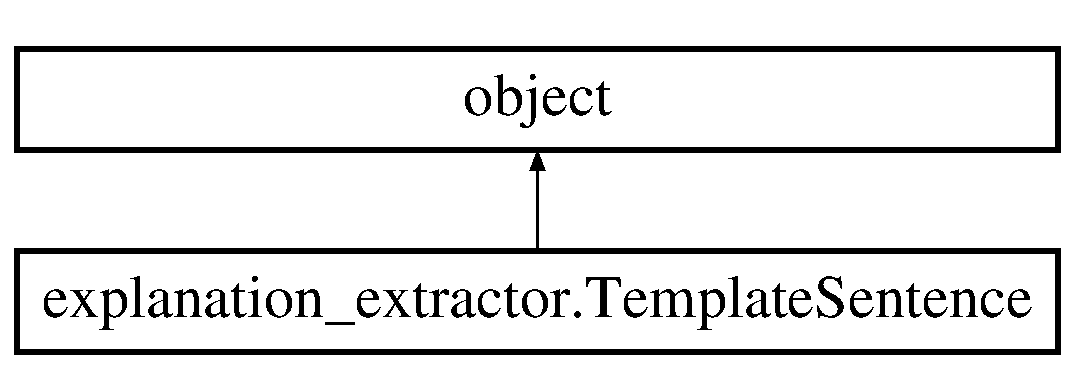
\includegraphics[height=2.000000cm]{classexplanation__extractor_1_1_template_sentence}
\end{center}
\end{figure}
\subsection*{Public Member Functions}
\begin{DoxyCompactItemize}
\item 
def \hyperlink{classexplanation__extractor_1_1_template_sentence_a22ddd1b4767a1c72969c5c930cbda078}{\+\_\+\+\_\+init\+\_\+\+\_\+}
\item 
def \hyperlink{classexplanation__extractor_1_1_template_sentence_a927b2a0ebda999c61956ae2a86871051}{update\+Variables}
\item 
def \hyperlink{classexplanation__extractor_1_1_template_sentence_a375ab886f8b7e3c675f092af6bae1c9b}{get\+Sentence\+Fragments} (self)
\item 
def \hyperlink{classexplanation__extractor_1_1_template_sentence_ae5bcc65ffabbe8b633249977f7aa6be1}{\+\_\+\+\_\+str\+\_\+\+\_\+} (self)
\end{DoxyCompactItemize}
\subsection*{Public Attributes}
\begin{DoxyCompactItemize}
\item 
\hyperlink{classexplanation__extractor_1_1_template_sentence_a32d502eb8958b05bc1bcd24711a88bef}{variables}
\item 
\hyperlink{classexplanation__extractor_1_1_template_sentence_a767650d37189470a42a43f23917ceafb}{var\+\_\+values}
\end{DoxyCompactItemize}


\subsection{Detailed Description}
\begin{DoxyVerb}encapsulates a single sentence of a template along with var substitution functionality
Also decides order of vars w.r.t. explanation
\end{DoxyVerb}
 

Definition at line 342 of file explanation\+\_\+extractor.\+py.



\subsection{Constructor \& Destructor Documentation}
\hypertarget{classexplanation__extractor_1_1_template_sentence_a22ddd1b4767a1c72969c5c930cbda078}{}\index{explanation\+\_\+extractor\+::\+Template\+Sentence@{explanation\+\_\+extractor\+::\+Template\+Sentence}!\+\_\+\+\_\+init\+\_\+\+\_\+@{\+\_\+\+\_\+init\+\_\+\+\_\+}}
\index{\+\_\+\+\_\+init\+\_\+\+\_\+@{\+\_\+\+\_\+init\+\_\+\+\_\+}!explanation\+\_\+extractor\+::\+Template\+Sentence@{explanation\+\_\+extractor\+::\+Template\+Sentence}}
\subsubsection[{\+\_\+\+\_\+init\+\_\+\+\_\+}]{\setlength{\rightskip}{0pt plus 5cm}def explanation\+\_\+extractor.\+Template\+Sentence.\+\_\+\+\_\+init\+\_\+\+\_\+ (
\begin{DoxyParamCaption}
\item[{}]{self, }
\item[{}]{sentence, }
\item[{}]{variables, }
\item[{}]{var\+\_\+assignments = {\ttfamily \{\}}}
\end{DoxyParamCaption}
)}\label{classexplanation__extractor_1_1_template_sentence_a22ddd1b4767a1c72969c5c930cbda078}


Definition at line 346 of file explanation\+\_\+extractor.\+py.



\subsection{Member Function Documentation}
\hypertarget{classexplanation__extractor_1_1_template_sentence_ae5bcc65ffabbe8b633249977f7aa6be1}{}\index{explanation\+\_\+extractor\+::\+Template\+Sentence@{explanation\+\_\+extractor\+::\+Template\+Sentence}!\+\_\+\+\_\+str\+\_\+\+\_\+@{\+\_\+\+\_\+str\+\_\+\+\_\+}}
\index{\+\_\+\+\_\+str\+\_\+\+\_\+@{\+\_\+\+\_\+str\+\_\+\+\_\+}!explanation\+\_\+extractor\+::\+Template\+Sentence@{explanation\+\_\+extractor\+::\+Template\+Sentence}}
\subsubsection[{\+\_\+\+\_\+str\+\_\+\+\_\+}]{\setlength{\rightskip}{0pt plus 5cm}def explanation\+\_\+extractor.\+Template\+Sentence.\+\_\+\+\_\+str\+\_\+\+\_\+ (
\begin{DoxyParamCaption}
\item[{}]{self}
\end{DoxyParamCaption}
)}\label{classexplanation__extractor_1_1_template_sentence_ae5bcc65ffabbe8b633249977f7aa6be1}


Definition at line 371 of file explanation\+\_\+extractor.\+py.

\hypertarget{classexplanation__extractor_1_1_template_sentence_a375ab886f8b7e3c675f092af6bae1c9b}{}\index{explanation\+\_\+extractor\+::\+Template\+Sentence@{explanation\+\_\+extractor\+::\+Template\+Sentence}!get\+Sentence\+Fragments@{get\+Sentence\+Fragments}}
\index{get\+Sentence\+Fragments@{get\+Sentence\+Fragments}!explanation\+\_\+extractor\+::\+Template\+Sentence@{explanation\+\_\+extractor\+::\+Template\+Sentence}}
\subsubsection[{get\+Sentence\+Fragments}]{\setlength{\rightskip}{0pt plus 5cm}def explanation\+\_\+extractor.\+Template\+Sentence.\+get\+Sentence\+Fragments (
\begin{DoxyParamCaption}
\item[{}]{self}
\end{DoxyParamCaption}
)}\label{classexplanation__extractor_1_1_template_sentence_a375ab886f8b7e3c675f092af6bae1c9b}
\begin{DoxyVerb}returns a list of variables and explanation extracted from predicate name
    that must be joined to obtain a full explanation
\end{DoxyVerb}
 

Definition at line 358 of file explanation\+\_\+extractor.\+py.

\hypertarget{classexplanation__extractor_1_1_template_sentence_a927b2a0ebda999c61956ae2a86871051}{}\index{explanation\+\_\+extractor\+::\+Template\+Sentence@{explanation\+\_\+extractor\+::\+Template\+Sentence}!update\+Variables@{update\+Variables}}
\index{update\+Variables@{update\+Variables}!explanation\+\_\+extractor\+::\+Template\+Sentence@{explanation\+\_\+extractor\+::\+Template\+Sentence}}
\subsubsection[{update\+Variables}]{\setlength{\rightskip}{0pt plus 5cm}def explanation\+\_\+extractor.\+Template\+Sentence.\+update\+Variables (
\begin{DoxyParamCaption}
\item[{}]{self, }
\item[{}]{var\+\_\+assignments = {\ttfamily \{\}}}
\end{DoxyParamCaption}
)}\label{classexplanation__extractor_1_1_template_sentence_a927b2a0ebda999c61956ae2a86871051}
\begin{DoxyVerb}returns list containing variables and strings to be joined \end{DoxyVerb}
 

Definition at line 355 of file explanation\+\_\+extractor.\+py.



\subsection{Member Data Documentation}
\hypertarget{classexplanation__extractor_1_1_template_sentence_a767650d37189470a42a43f23917ceafb}{}\index{explanation\+\_\+extractor\+::\+Template\+Sentence@{explanation\+\_\+extractor\+::\+Template\+Sentence}!var\+\_\+values@{var\+\_\+values}}
\index{var\+\_\+values@{var\+\_\+values}!explanation\+\_\+extractor\+::\+Template\+Sentence@{explanation\+\_\+extractor\+::\+Template\+Sentence}}
\subsubsection[{var\+\_\+values}]{\setlength{\rightskip}{0pt plus 5cm}explanation\+\_\+extractor.\+Template\+Sentence.\+var\+\_\+values}\label{classexplanation__extractor_1_1_template_sentence_a767650d37189470a42a43f23917ceafb}


Definition at line 349 of file explanation\+\_\+extractor.\+py.

\hypertarget{classexplanation__extractor_1_1_template_sentence_a32d502eb8958b05bc1bcd24711a88bef}{}\index{explanation\+\_\+extractor\+::\+Template\+Sentence@{explanation\+\_\+extractor\+::\+Template\+Sentence}!variables@{variables}}
\index{variables@{variables}!explanation\+\_\+extractor\+::\+Template\+Sentence@{explanation\+\_\+extractor\+::\+Template\+Sentence}}
\subsubsection[{variables}]{\setlength{\rightskip}{0pt plus 5cm}explanation\+\_\+extractor.\+Template\+Sentence.\+variables}\label{classexplanation__extractor_1_1_template_sentence_a32d502eb8958b05bc1bcd24711a88bef}


Definition at line 348 of file explanation\+\_\+extractor.\+py.



The documentation for this class was generated from the following file\+:\begin{DoxyCompactItemize}
\item 
\hyperlink{explanation__extractor_8py}{explanation\+\_\+extractor.\+py}\end{DoxyCompactItemize}

\chapter{File Documentation}
\hypertarget{demo__runner_8py}{}\section{demo\+\_\+runner.\+py File Reference}
\label{demo__runner_8py}\index{demo\+\_\+runner.\+py@{demo\+\_\+runner.\+py}}
\subsection*{Classes}
\begin{DoxyCompactItemize}
\item 
class \hyperlink{classdemo__runner_1_1_demo_runner}{demo\+\_\+runner.\+Demo\+Runner}
\end{DoxyCompactItemize}
\subsection*{Namespaces}
\begin{DoxyCompactItemize}
\item 
 \hyperlink{namespacedemo__runner}{demo\+\_\+runner}
\end{DoxyCompactItemize}

\hypertarget{dist__metric__eqn_8py}{}\section{dist\+\_\+metric\+\_\+eqn.\+py File Reference}
\label{dist__metric__eqn_8py}\index{dist\+\_\+metric\+\_\+eqn.\+py@{dist\+\_\+metric\+\_\+eqn.\+py}}
\subsection*{Namespaces}
\begin{DoxyCompactItemize}
\item 
 \hyperlink{namespacedist__metric__eqn}{dist\+\_\+metric\+\_\+eqn}
\end{DoxyCompactItemize}
\subsection*{Functions}
\begin{DoxyCompactItemize}
\item 
def \hyperlink{namespacedist__metric__eqn_ab4def04a832b446de3b516010c9d25c8}{dist\+\_\+metric\+\_\+eqn.\+distance\+Between\+Eqn} (fst\+\_\+eqn, snd\+\_\+eqn)
\item 
def \hyperlink{namespacedist__metric__eqn_a7c272f023cb7f03d89b02abfbe1e3db4}{dist\+\_\+metric\+\_\+eqn.\+ast\+Of\+Eqn} (eqn\+\_\+string)
\item 
def \hyperlink{namespacedist__metric__eqn_a0edcc8b6da256e87db3a3be211edd30c}{dist\+\_\+metric\+\_\+eqn.\+sanitize\+Eqn\+String} (equation)
\item 
def \hyperlink{namespacedist__metric__eqn_a885aa0745926a86faa53586adf1b96cd}{dist\+\_\+metric\+\_\+eqn.\+distance\+Of\+A\+S\+Ts} (fst\+\_\+tree, snd\+\_\+tree)
\item 
def \hyperlink{namespacedist__metric__eqn_a1257cacac74473c011cd73cc9ab42662}{dist\+\_\+metric\+\_\+eqn.\+compare\+Expressions\+Recursive}
\item 
def \hyperlink{namespacedist__metric__eqn_acc471149507b72a3ae90479ce8d1d530}{dist\+\_\+metric\+\_\+eqn.\+compute\+Subtree\+Weight}
\item 
def \hyperlink{namespacedist__metric__eqn_a1ed3fe178511ac2221f10e8b265616de}{dist\+\_\+metric\+\_\+eqn.\+compare\+Monomials} (fst\+\_\+mono, snd\+\_\+mono)
\item 
def \hyperlink{namespacedist__metric__eqn_a3c77142a78935fdb677e08c99072f75f}{dist\+\_\+metric\+\_\+eqn.\+is\+Const\+Term} (expr)
\item 
def \hyperlink{namespacedist__metric__eqn_a4b224f351734acf574055f60fe2414f9}{dist\+\_\+metric\+\_\+eqn.\+is\+Exponentiated\+Variable} (expr)
\item 
def \hyperlink{namespacedist__metric__eqn_a9accdb032b41a2b1f4c7d670140ff5d2}{dist\+\_\+metric\+\_\+eqn.\+is\+Variable\+Term} (expr)
\item 
def \hyperlink{namespacedist__metric__eqn_ab5f8a8fe7e017ea46cf425f103f9c745}{dist\+\_\+metric\+\_\+eqn.\+is\+Mono\+In\+Standard\+Form} (expr)
\item 
def \hyperlink{namespacedist__metric__eqn_adfb57d0eb8cb656d890cfeac71aff1dd}{dist\+\_\+metric\+\_\+eqn.\+is\+Monomial} (expr)
\item 
def \hyperlink{namespacedist__metric__eqn_a23d8ec2868beb4e11d36b4611e2c7f6e}{dist\+\_\+metric\+\_\+eqn.\+iterate\+Pairs} (some\+\_\+list)
\item 
def \hyperlink{namespacedist__metric__eqn_ae8046557c5972d9ffd9c77d25e5abd49}{dist\+\_\+metric\+\_\+eqn.\+find\+Contrasting\+Cases} (generated\+\_\+probs\+\_\+list, max\+\_\+distance)
\item 
def \hyperlink{namespacedist__metric__eqn_af77246294f5fbb93d6788c455ae1f827}{dist\+\_\+metric\+\_\+eqn.\+include\+By\+Heuristic} (generated\+\_\+probs\+\_\+list, heuristic)
\item 
def \hyperlink{namespacedist__metric__eqn_a3eb6af1e2f9fc3cad956ad7ecb9852d2}{dist\+\_\+metric\+\_\+eqn.\+exclude\+By\+Heuristic} (generated\+\_\+probs\+\_\+list, heuristic)
\item 
def \hyperlink{namespacedist__metric__eqn_ada852c0f3c349db11cf1b4ea5da89e74}{dist\+\_\+metric\+\_\+eqn.\+alternate\+Contrasting\+Cases} (generated\+\_\+problems\+\_\+list, max\+\_\+distance)
\item 
def \hyperlink{namespacedist__metric__eqn_ad6e4e1db6faa529b0986aad5954f969b}{dist\+\_\+metric\+\_\+eqn.\+main} ()
\end{DoxyCompactItemize}
\subsection*{Variables}
\begin{DoxyCompactItemize}
\item 
int \hyperlink{namespacedist__metric__eqn_ac65c2f73b8bc8a1d97a09c48efc58937}{dist\+\_\+metric\+\_\+eqn.\+D\+I\+F\+F\+\_\+\+M\+O\+N\+O\+S\+\_\+\+P\+E\+N\+A\+L\+T\+Y} = 1
\item 
int \hyperlink{namespacedist__metric__eqn_a01d67ad0b779a93cdf541bc1ffd0cf2c}{dist\+\_\+metric\+\_\+eqn.\+D\+I\+F\+F\+\_\+\+N\+O\+D\+E\+\_\+\+T\+Y\+P\+E\+\_\+\+P\+E\+N\+A\+L\+T\+Y} = 2
\item 
int \hyperlink{namespacedist__metric__eqn_a230e03fde3fb3e89b8816b5ae0fdc4dc}{dist\+\_\+metric\+\_\+eqn.\+M\+A\+X\+\_\+\+D\+E\+P\+T\+H\+\_\+\+P\+E\+N\+A\+L\+T\+Y} = 4
\item 
list \hyperlink{namespacedist__metric__eqn_a684e63911b91cc150a8c6e7ace89ea78}{dist\+\_\+metric\+\_\+eqn.\+current\+\_\+depth} = \mbox{[}1\mbox{]}
\item 
list \hyperlink{namespacedist__metric__eqn_a6ed7ee3e88472aac349189bc8e620026}{dist\+\_\+metric\+\_\+eqn.\+all\+\_\+heuristics}
\end{DoxyCompactItemize}

\hypertarget{eqn__viz_8py}{}\section{eqn\+\_\+viz.\+py File Reference}
\label{eqn__viz_8py}\index{eqn\+\_\+viz.\+py@{eqn\+\_\+viz.\+py}}
\subsection*{Classes}
\begin{DoxyCompactItemize}
\item 
class \hyperlink{classeqn__viz_1_1_generated_problem}{eqn\+\_\+viz.\+Generated\+Problem}
\item 
class \hyperlink{classeqn__viz_1_1_generated_answer_set}{eqn\+\_\+viz.\+Generated\+Answer\+Set}
\item 
class \hyperlink{classeqn__viz_1_1_equation_step_parser}{eqn\+\_\+viz.\+Equation\+Step\+Parser}
\item 
class \hyperlink{classeqn__viz_1_1_algebra_node}{eqn\+\_\+viz.\+Algebra\+Node}
\item 
class \hyperlink{classeqn__viz_1_1_math_problem_parser}{eqn\+\_\+viz.\+Math\+Problem\+Parser}
\item 
class \hyperlink{classeqn__viz_1_1_model_manager}{eqn\+\_\+viz.\+Model\+Manager}
\item 
class \hyperlink{classeqn__viz_1_1_answer_set_parser}{eqn\+\_\+viz.\+Answer\+Set\+Parser}
\item 
class \hyperlink{classeqn__viz_1_1_answer_set_manager}{eqn\+\_\+viz.\+Answer\+Set\+Manager}
\end{DoxyCompactItemize}
\subsection*{Namespaces}
\begin{DoxyCompactItemize}
\item 
 \hyperlink{namespaceeqn__viz}{eqn\+\_\+viz}
\end{DoxyCompactItemize}
\subsection*{Functions}
\begin{DoxyCompactItemize}
\item 
def \hyperlink{namespaceeqn__viz_a09faf0d0395a3e4f6075cce89ff0285d}{eqn\+\_\+viz.\+get\+Template\+Manager} ()
\item 
def \hyperlink{namespaceeqn__viz_a77840944e82440038b71417a8d7204b1}{eqn\+\_\+viz.\+compose\+Parsers} (left, middle, right)
\item 
def \hyperlink{namespaceeqn__viz_a993af6aa282c460f53ded3ad8c8b0b93}{eqn\+\_\+viz.\+peel\+Holds} (tokens)
\item 
def \hyperlink{namespaceeqn__viz_afb82e11030ed8435793bb5958189540d}{eqn\+\_\+viz.\+main} (cmd\+\_\+line\+\_\+args)
\item 
def \hyperlink{namespaceeqn__viz_a1ced7888f4e1050beff42555639b94ef}{eqn\+\_\+viz.\+get\+Cmd\+Line\+Args} ()
\end{DoxyCompactItemize}
\subsection*{Variables}
\begin{DoxyCompactItemize}
\item 
tuple \hyperlink{namespaceeqn__viz_a0e6b1a683d662dd566b0cece84265fae}{eqn\+\_\+viz.\+Heuristic} = namedtuple(\textquotesingle{}Heuristic\textquotesingle{}, \mbox{[}\textquotesingle{}name\textquotesingle{}, \textquotesingle{}priority\textquotesingle{}, \textquotesingle{}trigger\textquotesingle{}\mbox{]})
\item 
tuple \hyperlink{namespaceeqn__viz_a1bea532f61715c9742cbbe0bef8e5121}{eqn\+\_\+viz.\+heur\+\_\+file} = open(\textquotesingle{}list\+\_\+of\+\_\+heuristics.\+txt\textquotesingle{}, \textquotesingle{}r\textquotesingle{})
\item 
dictionary \hyperlink{namespaceeqn__viz_a8017c4f105a541309fcf639e7925a88b}{eqn\+\_\+viz.\+H\+E\+U\+R\+\_\+\+I\+N\+F\+O} = \{\}
\item 
\hyperlink{namespaceeqn__viz_af2da9273cfc3d8dc9ce1f05558cbc838}{eqn\+\_\+viz.\+T\+E\+M\+P\+L\+A\+T\+E\+\_\+\+M\+A\+N\+A\+G\+E\+R} = None
\item 
tuple \hyperlink{namespaceeqn__viz_a5e65c3435a54324008033d990d858e72}{eqn\+\_\+viz.\+number\+\_\+parser} = Word(nums + \textquotesingle{}-\/\textquotesingle{})
\item 
tuple \hyperlink{namespaceeqn__viz_ad9dc00d4b3c0b288d0f204937297b179}{eqn\+\_\+viz.\+word\+\_\+parser} = Word(alphas)
\item 
string \hyperlink{namespaceeqn__viz_aa3f9b7373809e0e391e1383fd878b616}{eqn\+\_\+viz.\+node\+\_\+parser} = \textquotesingle{}id(\textquotesingle{}
\item 
\hyperlink{namespaceeqn__viz_ae1292d980053c2a15be129430ee3ebb1}{eqn\+\_\+viz.\+coeff} = number\+\_\+parser
\item 
\hyperlink{namespaceeqn__viz_a1376f5d1deece596253f6876d746a500}{eqn\+\_\+viz.\+deg} = number\+\_\+parser
\item 
\hyperlink{namespaceeqn__viz_aa45f3f597ca3ecacab90d141137afe1c}{eqn\+\_\+viz.\+poly\+\_\+parser} = number\+\_\+parser
\item 
string \hyperlink{namespaceeqn__viz_a7bf2f0fb75b2d7a493e3ebf9cf2f580e}{eqn\+\_\+viz.\+time\+\_\+parser} = \textquotesingle{}time(\textquotesingle{}
\item 
string \hyperlink{namespaceeqn__viz_ab821f1efc209d98cc2cbfce1f818acbc}{eqn\+\_\+viz.\+action\+\_\+parser} = \textquotesingle{}selected\+Heuristic(\textquotesingle{}
\item 
string \hyperlink{namespaceeqn__viz_a854e9036019062010a0620dca4adcf5f}{eqn\+\_\+viz.\+factora\+\_\+parser} = \textquotesingle{}factor1(\textquotesingle{}
\item 
string \hyperlink{namespaceeqn__viz_a830b341130da6861c90efd9ac0858486}{eqn\+\_\+viz.\+factorb\+\_\+parser} = \textquotesingle{}factor2(\textquotesingle{}
\item 
string \hyperlink{namespaceeqn__viz_addfe6dbd1f7e4817decc2f392291d743}{eqn\+\_\+viz.\+factorc\+\_\+parser} = \textquotesingle{}factor3(\textquotesingle{}
\item 
string \hyperlink{namespaceeqn__viz_a17e1b80ac39bb02b3448c7cc9e5e7821}{eqn\+\_\+viz.\+factord\+\_\+parser} = \textquotesingle{}factor4(\textquotesingle{}
\item 
string \hyperlink{namespaceeqn__viz_a28dbd804760bc7a217c14254976e5575}{eqn\+\_\+viz.\+refer\+\_\+to\+\_\+\+Parser} = \textquotesingle{}refer\+To(\textquotesingle{}
\item 
string \hyperlink{namespaceeqn__viz_ab4bb266f8ba35459c0d095bcffadbad4}{eqn\+\_\+viz.\+soln\+\_\+parser} = \textquotesingle{}solution\+Value(\textquotesingle{}
\item 
string \hyperlink{namespaceeqn__viz_aacd332e3c02218eb9ae4ec66a3e31fd0}{eqn\+\_\+viz.\+substitute\+\_\+parser} = \textquotesingle{}substituted\+Degree(\textquotesingle{}
\item 
string \hyperlink{namespaceeqn__viz_a7a7eda2f6b22edf43034366ee5b0e433}{eqn\+\_\+viz.\+binary\+\_\+operand\+\_\+parser} = \textquotesingle{}selected\+Heur\+Operands(\textquotesingle{}
\item 
string \hyperlink{namespaceeqn__viz_a0eb89bf8984a1b19989d2031cae402a6}{eqn\+\_\+viz.\+unary\+\_\+operand\+\_\+parser} = \textquotesingle{}selected\+Heur\+Operands(\textquotesingle{}
\item 
tuple \hyperlink{namespaceeqn__viz_a716255e5870a531e1bfc6d184278bc8d}{eqn\+\_\+viz.\+wrap\+Node\+Fact} = lambdaparser\+:compose\+Parsers(\textquotesingle{}fact(\textquotesingle{}+ node\+\_\+parser + \textquotesingle{},\textquotesingle{}, parser, \textquotesingle{})\textquotesingle{})
\item 
tuple \hyperlink{namespaceeqn__viz_aa72fea76ddf1127d6dbcb77d7c76c63d}{eqn\+\_\+viz.\+wrap\+Poly\+Fact} = lambdaparser\+:compose\+Parsers(\textquotesingle{}fact(\textquotesingle{}+ poly\+\_\+parser + \textquotesingle{},\textquotesingle{}, parser, \textquotesingle{})\textquotesingle{})
\item 
tuple \hyperlink{namespaceeqn__viz_adf51f57cbfcd953ec98550b85dcc3d0c}{eqn\+\_\+viz.\+wrap\+Key\+Value\+Pair} = lambdaparser\+:compose\+Parsers(\textquotesingle{}node\+Field(\textquotesingle{}, parser, \textquotesingle{})\textquotesingle{})
\item 
tuple \hyperlink{namespaceeqn__viz_afead5f7b23dd83ce8d2c7092b9887606}{eqn\+\_\+viz.\+wrap\+With\+Monomial} = lambdaparser\+:compose\+Parsers(\textquotesingle{}mono(\textquotesingle{}, parser, \textquotesingle{})\textquotesingle{})
\item 
tuple \hyperlink{namespaceeqn__viz_a66245c2eeb429b7809bc02fc6852d0ec}{eqn\+\_\+viz.\+wrap\+With\+Holds} = lambdafluent\+:compose\+Parsers(\textquotesingle{}holds(\textquotesingle{},time\+\_\+parser, \textquotesingle{},\textquotesingle{} + fluent + \textquotesingle{})\textquotesingle{})
\item 
tuple \hyperlink{namespaceeqn__viz_aaabd8c0ea3860c55e9022abed90dab61}{eqn\+\_\+viz.\+word\+\_\+word\+\_\+parser} = compose\+Parsers(word\+\_\+parser, \textquotesingle{},\textquotesingle{} , word\+\_\+parser)
\item 
tuple \hyperlink{namespaceeqn__viz_ae9d46b4030dff778fd4a908af15b1461}{eqn\+\_\+viz.\+number\+\_\+number\+\_\+parser} = compose\+Parsers(number\+\_\+parser, \textquotesingle{},\textquotesingle{} , number\+\_\+parser)
\item 
tuple \hyperlink{namespaceeqn__viz_a125896c7d7db5d4f150b2b6699176c2a}{eqn\+\_\+viz.\+word\+\_\+number\+\_\+parser} = compose\+Parsers(word\+\_\+parser, \textquotesingle{},\textquotesingle{} , number\+\_\+parser)
\item 
tuple \hyperlink{namespaceeqn__viz_ade698a80074d34a48d27d50b0b6faafc}{eqn\+\_\+viz.\+word\+\_\+node\+\_\+parser} = compose\+Parsers(word\+\_\+parser, \textquotesingle{},\textquotesingle{} , node\+\_\+parser)
\item 
tuple \hyperlink{namespaceeqn__viz_aff7c3fc95453270d356d2c9fef5be210}{eqn\+\_\+viz.\+wrap\+In\+Key\+Value\+And\+Fact} = lambdaparser\+:wrap\+With\+Holds(wrap\+Node\+Fact(wrap\+Key\+Value\+Pair(parser)))
\item 
tuple \hyperlink{namespaceeqn__viz_a80772625f40909e83c3baefb38694d27}{eqn\+\_\+viz.\+type\+\_\+parser} = wrap\+In\+Key\+Value\+And\+Fact(word\+\_\+word\+\_\+parser)
\item 
tuple \hyperlink{namespaceeqn__viz_aa7fc0cae83db0b5d1e6d5c5842cea401}{eqn\+\_\+viz.\+deg\+\_\+coeff\+\_\+parser} = wrap\+In\+Key\+Value\+And\+Fact(word\+\_\+number\+\_\+parser)
\item 
tuple \hyperlink{namespaceeqn__viz_a333b4ac72b3d28145584b60f44dc5230}{eqn\+\_\+viz.\+child\+\_\+parser} = wrap\+In\+Key\+Value\+And\+Fact(word\+\_\+node\+\_\+parser)
\item 
string \hyperlink{namespaceeqn__viz_adb85cfac07b72248b7de0626b8e31bff}{eqn\+\_\+viz.\+applicable\+\_\+heur\+\_\+parser} = \textquotesingle{}applicable\+Heuristic(\textquotesingle{}
\item 
list \hyperlink{namespaceeqn__viz_a7be3eddfb6de11856410a9b26fc4a701}{eqn\+\_\+viz.\+all\+\_\+parsers} = \mbox{[} type\+\_\+parser, child\+\_\+parser, deg\+\_\+coeff\+\_\+parser, action\+\_\+parser, binary\+\_\+operand\+\_\+parser, unary\+\_\+operand\+\_\+parser, applicable\+\_\+heur\+\_\+parser\mbox{]}
\item 
list \hyperlink{namespaceeqn__viz_a87c2b92574d4b106ac2b4a2627a5824b}{eqn\+\_\+viz.\+factor\+\_\+parsers} = \mbox{[}factora\+\_\+parser, factorb\+\_\+parser, factorc\+\_\+parser, factord\+\_\+parser, refer\+\_\+to\+\_\+\+Parser, soln\+\_\+parser, substitute\+\_\+parser\mbox{]}
\item 
dictionary \hyperlink{namespaceeqn__viz_a9377a4d68a694cfe5b8fd887d7d4f045}{eqn\+\_\+viz.\+op\+\_\+symbols} = \{\textquotesingle{}add\textquotesingle{} \+: \textquotesingle{}+\textquotesingle{} , \textquotesingle{}div\textquotesingle{} \+: \textquotesingle{}/\textquotesingle{} , \textquotesingle{}mul\textquotesingle{} \+: \textquotesingle{}$\ast$\textquotesingle{} , \textquotesingle{}neg\textquotesingle{} \+: \textquotesingle{}-\/\textquotesingle{}\}
\end{DoxyCompactItemize}

\hypertarget{explanation__extractor_8py}{}\section{explanation\+\_\+extractor.\+py File Reference}
\label{explanation__extractor_8py}\index{explanation\+\_\+extractor.\+py@{explanation\+\_\+extractor.\+py}}
\subsection*{Classes}
\begin{DoxyCompactItemize}
\item 
class \hyperlink{classexplanation__extractor_1_1_explanation_manager}{explanation\+\_\+extractor.\+Explanation\+Manager}
\item 
class \hyperlink{classexplanation__extractor_1_1_explanation_template}{explanation\+\_\+extractor.\+Explanation\+Template}
\item 
class \hyperlink{classexplanation__extractor_1_1_template_sentence}{explanation\+\_\+extractor.\+Template\+Sentence}
\end{DoxyCompactItemize}
\subsection*{Namespaces}
\begin{DoxyCompactItemize}
\item 
 \hyperlink{namespaceexplanation__extractor}{explanation\+\_\+extractor}
\end{DoxyCompactItemize}
\subsection*{Functions}
\begin{DoxyCompactItemize}
\item 
def \hyperlink{namespaceexplanation__extractor_a7d686ee54e958cf12fdf7f9522b8bae3}{explanation\+\_\+extractor.\+get\+Template\+Manager} ()
\item 
def \hyperlink{namespaceexplanation__extractor_a7a90d19505230cd0706029001284f6a6}{explanation\+\_\+extractor.\+make\+Sanitized\+File} (file\+\_\+name)
\item 
def \hyperlink{namespaceexplanation__extractor_a5d9319a84e5b2170b092d43d5eff8af4}{explanation\+\_\+extractor.\+get\+Rules\+List\+From\+File} (file\+\_\+name)
\item 
def \hyperlink{namespaceexplanation__extractor_a003f30bfe39fe27dc9b5c95310ac37ab}{explanation\+\_\+extractor.\+parse\+Files} (file\+\_\+list)
\item 
def \hyperlink{namespaceexplanation__extractor_acbb78e911fb2dff47a068c333495b85d}{explanation\+\_\+extractor.\+parse\+Rules} ()
\item 
def \hyperlink{namespaceexplanation__extractor_a1208b0a7c420f414703614c42083ed8f}{explanation\+\_\+extractor.\+convert\+From\+Camel\+Case} (name)
\begin{DoxyCompactList}\small\item\em convert predicate name from camelcase to proper explanation \end{DoxyCompactList}\item 
def \hyperlink{namespaceexplanation__extractor_a3ca2de4ae7247867c29feb24c8b85f95}{explanation\+\_\+extractor.\+is\+Predicate} (condition)
\item 
def \hyperlink{namespaceexplanation__extractor_aecacec3e63255e9ee8653a73aa4416ce}{explanation\+\_\+extractor.\+is\+Heuristic\+Predicate} (predicate)
\item 
def \hyperlink{namespaceexplanation__extractor_a4de4948093b3eb32c6d46109dccca83d}{explanation\+\_\+extractor.\+is\+Skipped\+Predicate} (predicate)
\item 
def \hyperlink{namespaceexplanation__extractor_a7e792778552def0590947344cab0c799}{explanation\+\_\+extractor.\+filter\+Unused\+Conditions} (condition\+\_\+list)
\item 
def \hyperlink{namespaceexplanation__extractor_af072d9ebdb289310aac8bdfc6d18c45d}{explanation\+\_\+extractor.\+is\+Not\+Predicate} (condition)
\item 
def \hyperlink{namespaceexplanation__extractor_a3ff66fa3cac572ce943aadb6edd15faa}{explanation\+\_\+extractor.\+cond\+Is\+True\+Under\+Assignment} (cond, assign\+\_\+dict, mgr)
\item 
def \hyperlink{namespaceexplanation__extractor_a25cb9de50e008dc4719c37a755767f6c}{explanation\+\_\+extractor.\+get\+Level\+Two\+Predicates} (pred\+\_\+key)
\item 
def \hyperlink{namespaceexplanation__extractor_a97bc4aa83dd1f33e2055e0cd04280983}{explanation\+\_\+extractor.\+find\+Almost\+Matches\+Predicates} (pred\+\_\+key, model\+\_\+mgr)
\item 
def \hyperlink{namespaceexplanation__extractor_ad9ad528058d7d4a987217e34962fafa1}{explanation\+\_\+extractor.\+make\+Almost\+Fire\+Explanations} (pred\+\_\+key, model\+\_\+mgr)
\item 
def \hyperlink{namespaceexplanation__extractor_a245c76a80c6861aa9913a4c0ae657532}{explanation\+\_\+extractor.\+get\+All\+Satisfying\+Assignments} (conditions, model\+\_\+mgr)
\item 
def \hyperlink{namespaceexplanation__extractor_aa2ee543a844a51fd175237425613e637}{explanation\+\_\+extractor.\+find\+Assign} (cond\+\_\+list, mgr, assign, all\+\_\+assign)
\item 
def \hyperlink{namespaceexplanation__extractor_a6f48fd0483449ab57c4fc59bf46d9030}{explanation\+\_\+extractor.\+get\+All\+Compatible\+Matches} (cond, mgr, assign)
\item 
def \hyperlink{namespaceexplanation__extractor_ac4ebd7452ba8d0cd181de6ff9e826a97}{explanation\+\_\+extractor.\+is\+Compatible\+With} (ground\+\_\+dict, assign\+\_\+dict)
\item 
def \hyperlink{namespaceexplanation__extractor_a9ff3544e6f17deeb9ca26720176c3425}{explanation\+\_\+extractor.\+get\+Body\+Template\+Objects} (template)
\item 
def \hyperlink{namespaceexplanation__extractor_aceb0f7d5fe4722c93251a451c0887cf9}{explanation\+\_\+extractor.\+make\+List\+Of\+Almost\+Fire\+Conditions} (list\+\_\+of\+\_\+conditions)
\item 
def \hyperlink{namespaceexplanation__extractor_a83d1ad83ea4f6f229f663c8f2a6fec4e}{explanation\+\_\+extractor.\+get\+Test\+Model\+Mgr} ()
\item 
def \hyperlink{namespaceexplanation__extractor_ab07ea7707a24b1b7c5a0abfeab45c62d}{explanation\+\_\+extractor.\+main} (files)
\end{DoxyCompactItemize}
\subsection*{Variables}
\begin{DoxyCompactItemize}
\item 
dictionary \hyperlink{namespaceexplanation__extractor_a4e9dc7c262525efa41529de247ccb96a}{explanation\+\_\+extractor.\+heuristic\+\_\+to\+\_\+strategy}
\item 
tuple \hyperlink{namespaceexplanation__extractor_ac32b3e381284882ab71367fde9f5c646}{explanation\+\_\+extractor.\+strategy\+\_\+to\+\_\+heuristic} = defaultdict(list)
\item 
tuple \hyperlink{namespaceexplanation__extractor_a4f4d79f4f4c8925bd6353200232eb735}{explanation\+\_\+extractor.\+list\+\_\+of\+\_\+heuristics} = heuristic\+\_\+to\+\_\+strategy.\+keys()
\item 
\hyperlink{namespaceexplanation__extractor_add16cd790071f284854455eddfa329a1}{explanation\+\_\+extractor.\+T\+E\+M\+P\+L\+A\+T\+E\+\_\+\+M\+A\+N\+A\+G\+E\+R} = None
\item 
list \hyperlink{namespaceexplanation__extractor_a4df375151186067de08268d91ffe50f9}{explanation\+\_\+extractor.\+files\+\_\+to\+\_\+parse} = \mbox{[}\textquotesingle{}rules.\+lp\textquotesingle{}\mbox{]}
\end{DoxyCompactItemize}

\hypertarget{get__all__soln_8py}{}\section{get\+\_\+all\+\_\+soln.\+py File Reference}
\label{get__all__soln_8py}\index{get\+\_\+all\+\_\+soln.\+py@{get\+\_\+all\+\_\+soln.\+py}}
\subsection*{Namespaces}
\begin{DoxyCompactItemize}
\item 
 \hyperlink{namespaceget__all__soln}{get\+\_\+all\+\_\+soln}
\end{DoxyCompactItemize}
\subsection*{Variables}
\begin{DoxyCompactItemize}
\item 
tuple \hyperlink{namespaceget__all__soln_a8a2e063607a9c61cff17994a35c63763}{get\+\_\+all\+\_\+soln.\+opened\+\_\+file} = file(sys.\+argv\mbox{[}1\mbox{]}, \textquotesingle{}r\textquotesingle{})
\item 
tuple \hyperlink{namespaceget__all__soln_a8ec0c92a3d60c2d55db17bff79a7d724}{get\+\_\+all\+\_\+soln.\+inputs} = opened\+\_\+file.\+read()
\item 
tuple \hyperlink{namespaceget__all__soln_a7fa2bae5f6d50024567ab2b36196692b}{get\+\_\+all\+\_\+soln.\+output\+\_\+file} = file(\textquotesingle{}probs/\textquotesingle{}+str(index) + \textquotesingle{}.prob\textquotesingle{}, \textquotesingle{}w\textquotesingle{})
\end{DoxyCompactItemize}

\hypertarget{merge__solutions_8py}{}\section{merge\+\_\+solutions.\+py File Reference}
\label{merge__solutions_8py}\index{merge\+\_\+solutions.\+py@{merge\+\_\+solutions.\+py}}
\subsection*{Namespaces}
\begin{DoxyCompactItemize}
\item 
 \hyperlink{namespacemerge__solutions}{merge\+\_\+solutions}
\end{DoxyCompactItemize}
\subsection*{Functions}
\begin{DoxyCompactItemize}
\item 
def \hyperlink{namespacemerge__solutions_ad0fda986a1c53a874ed095ef12027877}{merge\+\_\+solutions.\+get\+J\+S\+O\+N\+Object\+From\+File} (file\+\_\+name)
\item 
def \hyperlink{namespacemerge__solutions_afdaea17f186be2b756193101925af3a5}{merge\+\_\+solutions.\+merge\+J\+S\+O\+N\+Objects} (fst\+\_\+obj, snd\+\_\+obj)
\item 
def \hyperlink{namespacemerge__solutions_a9433a06eec90ce10b69902cf0e17ff69}{merge\+\_\+solutions.\+write\+Object\+To\+J\+S\+O\+N\+File} (obj, file\+\_\+name)
\end{DoxyCompactItemize}
\subsection*{Variables}
\begin{DoxyCompactItemize}
\item 
tuple \hyperlink{namespacemerge__solutions_a1a4d70efbd1013729dbfce1d0c9ef25b}{merge\+\_\+solutions.\+fst\+\_\+obj} = get\+J\+S\+O\+N\+Object\+From\+File(first\+\_\+file)
\item 
tuple \hyperlink{namespacemerge__solutions_a5b10d08f2e1f7a3c0660a4350142c13d}{merge\+\_\+solutions.\+snd\+\_\+obj} = get\+J\+S\+O\+N\+Object\+From\+File(snd\+\_\+file)
\item 
tuple \hyperlink{namespacemerge__solutions_af6f16aad7bb6f378fbaaa508f8afd746}{merge\+\_\+solutions.\+new\+\_\+json\+\_\+obj} = merge\+J\+S\+O\+N\+Objects(fst\+\_\+obj, snd\+\_\+obj)
\end{DoxyCompactItemize}

\hypertarget{model__manager_8py}{}\section{model\+\_\+manager.\+py File Reference}
\label{model__manager_8py}\index{model\+\_\+manager.\+py@{model\+\_\+manager.\+py}}
\subsection*{Classes}
\begin{DoxyCompactItemize}
\item 
class \hyperlink{classmodel__manager_1_1_model_manager}{model\+\_\+manager.\+Model\+Manager}
\end{DoxyCompactItemize}
\subsection*{Namespaces}
\begin{DoxyCompactItemize}
\item 
 \hyperlink{namespacemodel__manager}{model\+\_\+manager}
\end{DoxyCompactItemize}

\hypertarget{parse__asp__rules_8py}{}\section{parse\+\_\+asp\+\_\+rules.\+py File Reference}
\label{parse__asp__rules_8py}\index{parse\+\_\+asp\+\_\+rules.\+py@{parse\+\_\+asp\+\_\+rules.\+py}}
\subsection*{Classes}
\begin{DoxyCompactItemize}
\item 
class \hyperlink{classparse__asp__rules_1_1_rule_listener}{parse\+\_\+asp\+\_\+rules.\+Rule\+Listener}
\end{DoxyCompactItemize}
\subsection*{Namespaces}
\begin{DoxyCompactItemize}
\item 
 \hyperlink{namespaceparse__asp__rules}{parse\+\_\+asp\+\_\+rules}
\end{DoxyCompactItemize}
\subsection*{Functions}
\begin{DoxyCompactItemize}
\item 
def \hyperlink{namespaceparse__asp__rules_a1078844be7f2009c8ec09b66f660070e}{parse\+\_\+asp\+\_\+rules.\+parse\+Rules\+From\+File} (file\+\_\+name)
\item 
def \hyperlink{namespaceparse__asp__rules_a5deac66595588966e7f7480630f15f27}{parse\+\_\+asp\+\_\+rules.\+main} ()
\end{DoxyCompactItemize}
\subsection*{Variables}
\begin{DoxyCompactItemize}
\item 
tuple \hyperlink{namespaceparse__asp__rules_acc4a48d78de76e3b65c2aa3ebba7e194}{parse\+\_\+asp\+\_\+rules.\+Predicate} = namedtuple(\textquotesingle{}Predicate\textquotesingle{}, \mbox{[}\textquotesingle{}name\textquotesingle{}, \textquotesingle{}args\textquotesingle{}, \textquotesingle{}arity\textquotesingle{}\mbox{]})
\item 
tuple \hyperlink{namespaceparse__asp__rules_a7385160dd946ac7f3eb5cd48b40a1287}{parse\+\_\+asp\+\_\+rules.\+Neg\+Predicate} = namedtuple(\textquotesingle{}Neg\+Predicate\textquotesingle{}, \mbox{[}\textquotesingle{}name\textquotesingle{}, \textquotesingle{}args\textquotesingle{}, \textquotesingle{}arity\textquotesingle{}\mbox{]})
\item 
tuple \hyperlink{namespaceparse__asp__rules_a14e0f083d2fb02ac073930c7d32fc056}{parse\+\_\+asp\+\_\+rules.\+Rule} = namedtuple(\textquotesingle{}Rule\textquotesingle{}, \mbox{[}\textquotesingle{}head\textquotesingle{}, \textquotesingle{}body\textquotesingle{}\mbox{]})
\item 
tuple \hyperlink{namespaceparse__asp__rules_ac4278713dc495679b30669abb0793c95}{parse\+\_\+asp\+\_\+rules.\+Comparison} = namedtuple(\textquotesingle{}Comparison\textquotesingle{}, \mbox{[}\textquotesingle{}left\textquotesingle{}, \textquotesingle{}comparator\textquotesingle{}\mbox{]} )
\item 
tuple \hyperlink{namespaceparse__asp__rules_ad6499631d0c32c55386ca6c1e97cf88f}{parse\+\_\+asp\+\_\+rules.\+Pred\+Count} = namedtuple(\textquotesingle{}Pred\+Count\textquotesingle{}, \mbox{[}\textquotesingle{}left\+\_\+count\textquotesingle{}, \textquotesingle{}predicate\textquotesingle{}, \textquotesingle{}conditions\textquotesingle{}, \textquotesingle{}right\+\_\+count\textquotesingle{}\mbox{]})
\end{DoxyCompactItemize}

\hypertarget{pred__parser_8py}{}\section{pred\+\_\+parser.\+py File Reference}
\label{pred__parser_8py}\index{pred\+\_\+parser.\+py@{pred\+\_\+parser.\+py}}
\subsection*{Namespaces}
\begin{DoxyCompactItemize}
\item 
 \hyperlink{namespacepred__parser}{pred\+\_\+parser}
\end{DoxyCompactItemize}
\subsection*{Functions}
\begin{DoxyCompactItemize}
\item 
def \hyperlink{namespacepred__parser_aafbae146acf181131bb122c749d70997}{pred\+\_\+parser.\+predicate\+String\+To\+Parsed\+Predicate} (string)
\item 
def \hyperlink{namespacepred__parser_af74de27d3d3628a01e182ff0082cb502}{pred\+\_\+parser.\+split\+On\+Outermost\+Parens} (string)
\item 
def \hyperlink{namespacepred__parser_a7e9dce7771bb530467ef4a68d11c7804}{pred\+\_\+parser.\+parse\+Predicate\+Arguments} (arg\+\_\+string)
\item 
def \hyperlink{namespacepred__parser_a8af17d45b99ad2593a1063c36162187a}{pred\+\_\+parser.\+pred\+Object\+To\+String} (pred\+\_\+obj)
\item 
def \hyperlink{namespacepred__parser_a29597ce97183f1be99e6a96d16d767db}{pred\+\_\+parser.\+get\+Time\+From\+Pred\+Object} (pred\+\_\+obj)
\item 
def \hyperlink{namespacepred__parser_a918636a789322106c44f3ab3a40c4eb3}{pred\+\_\+parser.\+find\+In\+Arg\+List} (pred\+\_\+obj, pred\+\_\+name)
\item 
def \hyperlink{namespacepred__parser_a97b4149316ed6221e074bffd1d58e43c}{pred\+\_\+parser.\+args\+To\+List\+Of\+Strings} (pred\+\_\+obj)
\item 
def \hyperlink{namespacepred__parser_a2a6fff2c8801ac4b209b04d97653a9d8}{pred\+\_\+parser.\+holds\+Object\+To\+Node\+Field\+Value} (holds\+\_\+pred)
\end{DoxyCompactItemize}
\subsection*{Variables}
\begin{DoxyCompactItemize}
\item 
tuple \hyperlink{namespacepred__parser_a3aacf710ab8840533bfdcc8f4e578421}{pred\+\_\+parser.\+Parsed\+Predicate} = namedtuple(\textquotesingle{}Parsed\+Predicate\textquotesingle{}, \mbox{[}\textquotesingle{}name\textquotesingle{}, \textquotesingle{}args\textquotesingle{}\mbox{]})
\item 
tuple \hyperlink{namespacepred__parser_af458c74fe479675c5d30a1dbd7375bed}{pred\+\_\+parser.\+Time} = namedtuple(\textquotesingle{}Time\textquotesingle{}, \mbox{[}\textquotesingle{}step\textquotesingle{}, \textquotesingle{}stream\textquotesingle{}\mbox{]})
\end{DoxyCompactItemize}

\hypertarget{_prolog_rules_lexer_8py}{}\section{Prolog\+Rules\+Lexer.\+py File Reference}
\label{_prolog_rules_lexer_8py}\index{Prolog\+Rules\+Lexer.\+py@{Prolog\+Rules\+Lexer.\+py}}
\subsection*{Classes}
\begin{DoxyCompactItemize}
\item 
class \hyperlink{class_prolog_rules_lexer_1_1_prolog_rules_lexer}{Prolog\+Rules\+Lexer.\+Prolog\+Rules\+Lexer}
\end{DoxyCompactItemize}
\subsection*{Namespaces}
\begin{DoxyCompactItemize}
\item 
 \hyperlink{namespace_prolog_rules_lexer}{Prolog\+Rules\+Lexer}
\end{DoxyCompactItemize}
\subsection*{Functions}
\begin{DoxyCompactItemize}
\item 
def \hyperlink{namespace_prolog_rules_lexer_a75ab514649304bfd58856564964681c0}{Prolog\+Rules\+Lexer.\+serialized\+A\+T\+N} ()
\end{DoxyCompactItemize}

\hypertarget{_prolog_rules_listener_8py}{}\section{Prolog\+Rules\+Listener.\+py File Reference}
\label{_prolog_rules_listener_8py}\index{Prolog\+Rules\+Listener.\+py@{Prolog\+Rules\+Listener.\+py}}
\subsection*{Classes}
\begin{DoxyCompactItemize}
\item 
class \hyperlink{class_prolog_rules_listener_1_1_prolog_rules_listener}{Prolog\+Rules\+Listener.\+Prolog\+Rules\+Listener}
\end{DoxyCompactItemize}
\subsection*{Namespaces}
\begin{DoxyCompactItemize}
\item 
 \hyperlink{namespace_prolog_rules_listener}{Prolog\+Rules\+Listener}
\end{DoxyCompactItemize}

\hypertarget{_prolog_rules_parser_8py}{}\section{Prolog\+Rules\+Parser.\+py File Reference}
\label{_prolog_rules_parser_8py}\index{Prolog\+Rules\+Parser.\+py@{Prolog\+Rules\+Parser.\+py}}
\subsection*{Classes}
\begin{DoxyCompactItemize}
\item 
class \hyperlink{class_prolog_rules_parser_1_1_prolog_rules_parser}{Prolog\+Rules\+Parser.\+Prolog\+Rules\+Parser}
\item 
class \hyperlink{class_prolog_rules_parser_1_1_prolog_rules_parser_1_1_prologcode_context}{Prolog\+Rules\+Parser.\+Prolog\+Rules\+Parser.\+Prologcode\+Context}
\item 
class \hyperlink{class_prolog_rules_parser_1_1_prolog_rules_parser_1_1_prologthing_context}{Prolog\+Rules\+Parser.\+Prolog\+Rules\+Parser.\+Prologthing\+Context}
\item 
class \hyperlink{class_prolog_rules_parser_1_1_prolog_rules_parser_1_1_fact_context}{Prolog\+Rules\+Parser.\+Prolog\+Rules\+Parser.\+Fact\+Context}
\item 
class \hyperlink{class_prolog_rules_parser_1_1_prolog_rules_parser_1_1_constraint_context}{Prolog\+Rules\+Parser.\+Prolog\+Rules\+Parser.\+Constraint\+Context}
\item 
class \hyperlink{class_prolog_rules_parser_1_1_prolog_rules_parser_1_1_somerule_context}{Prolog\+Rules\+Parser.\+Prolog\+Rules\+Parser.\+Somerule\+Context}
\item 
class \hyperlink{class_prolog_rules_parser_1_1_prolog_rules_parser_1_1_prologrule_context}{Prolog\+Rules\+Parser.\+Prolog\+Rules\+Parser.\+Prologrule\+Context}
\item 
class \hyperlink{class_prolog_rules_parser_1_1_prolog_rules_parser_1_1_guessrule_context}{Prolog\+Rules\+Parser.\+Prolog\+Rules\+Parser.\+Guessrule\+Context}
\item 
class \hyperlink{class_prolog_rules_parser_1_1_prolog_rules_parser_1_1_predcount_context}{Prolog\+Rules\+Parser.\+Prolog\+Rules\+Parser.\+Predcount\+Context}
\item 
class \hyperlink{class_prolog_rules_parser_1_1_prolog_rules_parser_1_1_predicate_context}{Prolog\+Rules\+Parser.\+Prolog\+Rules\+Parser.\+Predicate\+Context}
\item 
class \hyperlink{class_prolog_rules_parser_1_1_prolog_rules_parser_1_1_rulebody_context}{Prolog\+Rules\+Parser.\+Prolog\+Rules\+Parser.\+Rulebody\+Context}
\item 
class \hyperlink{class_prolog_rules_parser_1_1_prolog_rules_parser_1_1_condition_context}{Prolog\+Rules\+Parser.\+Prolog\+Rules\+Parser.\+Condition\+Context}
\item 
class \hyperlink{class_prolog_rules_parser_1_1_prolog_rules_parser_1_1_negpred_context}{Prolog\+Rules\+Parser.\+Prolog\+Rules\+Parser.\+Negpred\+Context}
\item 
class \hyperlink{class_prolog_rules_parser_1_1_prolog_rules_parser_1_1_comparator_context}{Prolog\+Rules\+Parser.\+Prolog\+Rules\+Parser.\+Comparator\+Context}
\item 
class \hyperlink{class_prolog_rules_parser_1_1_prolog_rules_parser_1_1_mathexpr_context}{Prolog\+Rules\+Parser.\+Prolog\+Rules\+Parser.\+Mathexpr\+Context}
\item 
class \hyperlink{class_prolog_rules_parser_1_1_prolog_rules_parser_1_1_args_context}{Prolog\+Rules\+Parser.\+Prolog\+Rules\+Parser.\+Args\+Context}
\item 
class \hyperlink{class_prolog_rules_parser_1_1_prolog_rules_parser_1_1_onearg_context}{Prolog\+Rules\+Parser.\+Prolog\+Rules\+Parser.\+Onearg\+Context}
\item 
class \hyperlink{class_prolog_rules_parser_1_1_prolog_rules_parser_1_1_atom_context}{Prolog\+Rules\+Parser.\+Prolog\+Rules\+Parser.\+Atom\+Context}
\item 
class \hyperlink{class_prolog_rules_parser_1_1_prolog_rules_parser_1_1_identifier_context}{Prolog\+Rules\+Parser.\+Prolog\+Rules\+Parser.\+Identifier\+Context}
\end{DoxyCompactItemize}
\subsection*{Namespaces}
\begin{DoxyCompactItemize}
\item 
 \hyperlink{namespace_prolog_rules_parser}{Prolog\+Rules\+Parser}
\end{DoxyCompactItemize}
\subsection*{Functions}
\begin{DoxyCompactItemize}
\item 
def \hyperlink{namespace_prolog_rules_parser_a55c266fd73ad3e2b856fa581489d8845}{Prolog\+Rules\+Parser.\+serialized\+A\+T\+N} ()
\end{DoxyCompactItemize}
\subsection*{Variables}
\begin{DoxyCompactItemize}
\item 
tuple \hyperlink{namespace_prolog_rules_parser_af188b237d1e6379d338e445d97efe14f}{Prolog\+Rules\+Parser.\+package} = globals()
\item 
tuple \hyperlink{namespace_prolog_rules_parser_aac8b33350217b52d41d2f03712a9a972}{Prolog\+Rules\+Parser.\+ischild} = len(package)
\end{DoxyCompactItemize}

\hypertarget{_r_e_a_d_m_e_8markdown}{}\section{R\+E\+A\+D\+M\+E.\+markdown File Reference}
\label{_r_e_a_d_m_e_8markdown}\index{R\+E\+A\+D\+M\+E.\+markdown@{R\+E\+A\+D\+M\+E.\+markdown}}

\hypertarget{totally__new__visualizer_8py}{}\section{totally\+\_\+new\+\_\+visualizer.\+py File Reference}
\label{totally__new__visualizer_8py}\index{totally\+\_\+new\+\_\+visualizer.\+py@{totally\+\_\+new\+\_\+visualizer.\+py}}
\subsection*{Classes}
\begin{DoxyCompactItemize}
\item 
class \hyperlink{classtotally__new__visualizer_1_1_equation_step_parser}{totally\+\_\+new\+\_\+visualizer.\+Equation\+Step\+Parser}
\begin{DoxyCompactList}\small\item\em Parses predicates related to one step of a solution trace contains the data members\+: var\+\_\+str -- what variable an equation should be expressed with node\+\_\+data -- dictionary containing all node info parsed strategy\+\_\+data -- parsed explanations for the different strategy classes. \end{DoxyCompactList}\item 
class \hyperlink{classtotally__new__visualizer_1_1_problem_parser}{totally\+\_\+new\+\_\+visualizer.\+Problem\+Parser}
\begin{DoxyCompactList}\small\item\em Handles the parsing of a single generated problem. \end{DoxyCompactList}\item 
class \hyperlink{classtotally__new__visualizer_1_1_answer_set_j_s_o_n_encoder}{totally\+\_\+new\+\_\+visualizer.\+Answer\+Set\+J\+S\+O\+N\+Encoder}
\item 
class \hyperlink{classtotally__new__visualizer_1_1_answer_set_manager}{totally\+\_\+new\+\_\+visualizer.\+Answer\+Set\+Manager}
\begin{DoxyCompactList}\small\item\em Store and separate all the answer sets in the input provided. \end{DoxyCompactList}\end{DoxyCompactItemize}
\subsection*{Namespaces}
\begin{DoxyCompactItemize}
\item 
 \hyperlink{namespacetotally__new__visualizer}{totally\+\_\+new\+\_\+visualizer}
\end{DoxyCompactItemize}
\subsection*{Functions}
\begin{DoxyCompactItemize}
\item 
def \hyperlink{namespacetotally__new__visualizer_aa58bcbc4c3c0a513fa8d58155d9d6e46}{totally\+\_\+new\+\_\+visualizer.\+main} (cmd\+\_\+line\+\_\+args)
\item 
def \hyperlink{namespacetotally__new__visualizer_a5ed81f6c9d94b6894d3ba36844436f9e}{totally\+\_\+new\+\_\+visualizer.\+get\+Cmd\+Line\+Args} ()
\end{DoxyCompactItemize}
\subsection*{Variables}
\begin{DoxyCompactItemize}
\item 
dictionary \hyperlink{namespacetotally__new__visualizer_a3dd0f4daa013b2acf2fbd1f7aa0ad07c}{totally\+\_\+new\+\_\+visualizer.\+op\+\_\+symbols} = \{\textquotesingle{}add\textquotesingle{} \+: \textquotesingle{}+\textquotesingle{} , \textquotesingle{}div\textquotesingle{} \+: \textquotesingle{}/\textquotesingle{} , \textquotesingle{}mul\textquotesingle{} \+: \textquotesingle{}$\ast$\textquotesingle{} , \textquotesingle{}neg\textquotesingle{} \+: \textquotesingle{}-\/\textquotesingle{}\}
\item 
list \hyperlink{namespacetotally__new__visualizer_ab706e5502043e33aaccc4cd5db3a11a8}{totally\+\_\+new\+\_\+visualizer.\+factor\+\_\+predicates} = \mbox{[}\textquotesingle{}factor\textquotesingle{} + n for n in list(\textquotesingle{}1234\textquotesingle{})\mbox{]}
\item 
dictionary \hyperlink{namespacetotally__new__visualizer_ac35b4d88f3973e9437d26d620f6404d3}{totally\+\_\+new\+\_\+visualizer.\+factor\+\_\+name\+\_\+dict} = \{\textquotesingle{}factor1\textquotesingle{}\+:\textquotesingle{}F\+A\+C\+T\+O\+R\+A\textquotesingle{} , \textquotesingle{}factor2\textquotesingle{}\+:\textquotesingle{}F\+A\+C\+T\+O\+R\+B\textquotesingle{}, \textquotesingle{}factor3\textquotesingle{}\+:\textquotesingle{}F\+A\+C\+T\+O\+R\+X\textquotesingle{}, \textquotesingle{}factor4\textquotesingle{}\+:\textquotesingle{}F\+A\+C\+T\+O\+R\+Y\textquotesingle{} \}
\item 
list \hyperlink{namespacetotally__new__visualizer_a0336db197e4d6b0cc49dd792fa21d890}{totally\+\_\+new\+\_\+visualizer.\+all\+\_\+strategies} = \mbox{[}\textquotesingle{}cancel\textquotesingle{}, \textquotesingle{}combine\textquotesingle{}, \textquotesingle{}rearrange\textquotesingle{}, \textquotesingle{}move\textquotesingle{}, \textquotesingle{}expand\textquotesingle{}\mbox{]}
\item 
tuple \hyperlink{namespacetotally__new__visualizer_a69a6b4328317f3ea8abc150eafbda370}{totally\+\_\+new\+\_\+visualizer.\+Generated\+Step} = namedtuple(\textquotesingle{}Generated\+Step\textquotesingle{}, \mbox{[}\textquotesingle{}equation\+\_\+string\textquotesingle{}, \textquotesingle{}step\+\_\+data\textquotesingle{}\mbox{]})
\item 
tuple \hyperlink{namespacetotally__new__visualizer_ab9dc95295259f8165e1fdf15f954d2b1}{totally\+\_\+new\+\_\+visualizer.\+Generated\+Solution} = namedtuple(\textquotesingle{}Generated\+Solution\textquotesingle{}, \mbox{[}\textquotesingle{}problem\+\_\+string\textquotesingle{}, \textquotesingle{}solution\+\_\+steps\textquotesingle{}\mbox{]})
\end{DoxyCompactItemize}

\hypertarget{translate__tree__nodes_8py}{}\section{translate\+\_\+tree\+\_\+nodes.\+py File Reference}
\label{translate__tree__nodes_8py}\index{translate\+\_\+tree\+\_\+nodes.\+py@{translate\+\_\+tree\+\_\+nodes.\+py}}
\subsection*{Classes}
\begin{DoxyCompactItemize}
\item 
class \hyperlink{classtranslate__tree__nodes_1_1_algebra_node}{translate\+\_\+tree\+\_\+nodes.\+Algebra\+Node}
\end{DoxyCompactItemize}
\subsection*{Namespaces}
\begin{DoxyCompactItemize}
\item 
 \hyperlink{namespacetranslate__tree__nodes}{translate\+\_\+tree\+\_\+nodes}
\end{DoxyCompactItemize}
\subsection*{Functions}
\begin{DoxyCompactItemize}
\item 
def \hyperlink{namespacetranslate__tree__nodes_a0fa22892537d9cffeac49eb6f9aa4307}{translate\+\_\+tree\+\_\+nodes.\+get\+Translations\+For\+Node\+Data} (node\+\_\+data)
\item 
def \hyperlink{namespacetranslate__tree__nodes_a51a50c054c1657eab607eab3e5a82863}{translate\+\_\+tree\+\_\+nodes.\+dict\+To\+Algebra\+Node\+Repr} (node\+\_\+dict, node\+\_\+id)
\end{DoxyCompactItemize}

%--- End generated contents ---

% Index
\backmatter
\newpage
\phantomsection
\clearemptydoublepage
\addcontentsline{toc}{chapter}{Index}
\printindex

\end{document}
